%% =====================================================================
%%  Honours Dissertation --- CITS4010
%%  Marc Labouchardiere (23857377)
%%  Supervisor: Dr Jin B. Hong --- Department of CSSE, UWA
%%
%%  Boilerplate built on the UWA cshonours class (title page reworked to
%%  add the UWA crest and a supervisor line, in the style of a recent
%%  honours thesis). Compile with:  latexmk -pdf dissertation.tex
%%
%%  SKELETON (2026-08-12): chapter/section structure per the 11-Aug
%%  meeting rulings (supervisor decision register V5--V7) --- the research
%%  question decomposed into capture / model / evaluate, the inherited
%%  simulator moved to a Background chapter, sensitivity analysis as the
%%  results preamble. Headers only; argued prose is a separate
%%  voice-gated pass per section.
%% =====================================================================
\documentclass{cshonours}

% IEEE numeric referencing (Marc's ruling, 2026-08-16), matching the
% lit review. natbib runs in numbers mode so the \citep/\citet calls in
% the prose keep working, rendering [4] / Author [4]. Style is ieeetr
% (in this TeX Live install); swap to IEEEtran.bst at submission if the
% polished IEEE list is wanted --- the calls need no change.
\bibliographystyle{ieeetr}

% --- packages ---------------------------------------------------------
\usepackage{graphicx}          % UWA crest on the title page + figures
\usepackage{amsmath}
\usepackage{amssymb}\usepackage{pifont}      % \ding ticks (\propmet) in the property and appendix tables
\usepackage{array}            % ragged-right p-columns in the appendix tables
\usepackage{booktabs}          % nicer tables (\toprule, \midrule ...)
\usepackage[table]{xcolor}     % \rowcolor / \cellcolor for tab:mtd-metrics (zebra rows, greys grammar)
\usepackage{multirow}          % rotated row-group labels in tab:mtd-metrics
\usepackage{placeins}          % \FloatBarrier: a section's floats stay in it (2026-09-24)
\usepackage{float}             % [H] for ch5's PLACEHOLDER floats only --- see below
% ch5's floats are placeholder boxes with no prose between them, so the
% float queue flushed ahead of the headings and every sensitivity figure
% rendered BEFORE the subsection it belongs to (Marc, 2026-09-09: "the
% figures are not in the right place ... should be under the subsection").
% Fig. 5.1-5.4 landed on pp. 28-29 against subsections on p. 30; 5.4.1-5.4.3
% all sat on p. 37 with their figures on pp. 34-36. [H] pins each box under
% its own heading so the visual argument can be READ IN POSITION, which is
% the whole purpose of the placeholder pass. REVERT each [H] to [htbp] as
% that subsection's prose lands --- with text to flow around, [htbp] is the
% right specifier and [H] would strand whitespace.
% --- house table style (docs/workflows/figure_table_conventions.md §k) --
% Every table float opens with \tablestyle: one type size, unit row
% height, zebra rows in the greys grammar (\rowcolors numbers the header
% row 1 and shades even rows, so the first body row is shaded; booktabs'
% \toprule/\midrule do not count as rows but \cmidrule DOES --- never put
% one inside a striped body, it shifts the stripes). Row-group labels are set
% rotated with \rowgroup{<rows>}{<label>} in the group's LAST row
% (multirow's negative-span idiom, which is what makes the label sit on
% top of the shading). P{<width>} is a ragged-right paragraph column;
% never a bare p{}, whose justified cells open word gaps.
\newcolumntype{P}[1]{>{\raggedright\arraybackslash}p{#1}}
\newcommand{\tablestyle}{\footnotesize\renewcommand{\arraystretch}{1.0}\rowcolors{2}{}{black!5}}
\newcommand{\rowgroup}[2]{\multirow{-#1}{*}{\smash{\rotatebox{90}{\emph{#2}}}}}
% Group rows keep the stripes (Marc, 2026-10-01: "stripes everywhere"). A group
% row is unshaded and restarts the count, so its first member is shaded like
% the first body row of a flat table: \grouprow{<ncols>}{<label>} for a label
% row; \rowcolor{white}\grouplabel{<label>} & ... for a group row with values.
\newcommand{\grouplabel}[1]{\emph{#1}\global\rownum=1\relax}
\newcommand{\grouprow}[2]{\rowcolor{white}\multicolumn{#1}{@{}l}{\grouplabel{#2}}}
% Feature-matrix heads: a column label rotated 90 degrees, one or two
% lines (break with \\), bottom-aligned so every head sits on the rule.
% Same mechanism as \rowgroup, turned for columns (Table 3.3, 2026-09-07).
\newcommand{\rothead}[1]{\rotatebox{90}{\begin{tabular}[b]{@{}l@{}}#1\end{tabular}}}
% Property-matrix marks (Table 3.3 and its ch7 return): met = tick,
% the genre's own mark for present (conventions §e1); stand-in = a
% small dot, "they did something here, as opposed to nothing" (Marc,
% 2026-09-07 --- the Harvey half read as "the lineage does it all"; the
% greyed ring and then the tilde were retired the same day, the tilde
% as "too much visual space"). Rendered: $\cdot$ vanishes on the shaded
% rows; \textbullet at 0.55 reads as a clean small dot.
% Placeholder float box --- SCAFFOLDING for the figures-first drafting pass
% (2026-09-09). Every planned float in ch5 is present as a framed box with its
% intended caption, so the chapter's visual argument can be read and cut before
% any prose is written (writing guide: figures, then captions written long,
% then text). Replacing a placeholder is one line: swap \placeholderbox for
% \includegraphics{fig_5-...}. Delete this macro when the last one is replaced.
\newcommand{\placeholderbox}[2]{%
  \setlength{\fboxsep}{0pt}%
  \fbox{\parbox[c][#1][c]{\dimexpr\textwidth-2\fboxrule\relax}{%
    \centering\footnotesize\itshape\textcolor{black!55}{#2}}}}
% [CH3 REDRAFT ROUND 51, 2026-10-02, marks] RULED (Marc, mock-up set 1): tick / P / cross. "Nothing needs a mark": blank means not applicable and a dash not reported (results presentation standard), so a property the model lacks is a cross. P over the tilde ("doesn't read like anything"). pifont glyphs, one family.
\newcommand{\propmet}{\ding{51}}
\newcommand{\propnone}{\ding{55}}
% [CH3 SCRUTINY 2026-09-30, T3] partial mark enlarged from 0.55 to full size: at 0.55 it printed as a full stop (p. 14). Marc's dot kept (66456ce3).
% [CH3 REDRAFT ROUND 50, 2026-10-02, Table 3.3 marks] RULED (Marc): the dot "just reads like black dots on a page"; the CS reader's pattern recognition needs tick / tilde / blank. Tilde as the maths \sim (centred, full height; \textasciitilde prints raised and small). Overturns 66456ce3's dot.
\newcommand{\propstandin}{P}
% Float-page threshold, raised from the class's 0.5 (the Figure 2.1 trap,
% worked around twice with [t]; Tables 2.4 + 2.5 fell into it as a pair on
% 2026-09-05): a float, or a run of them, now needs 80 % of the text height
% before it is given a page of its own. topfraction is raised with it so
% that no float sits in the gap between the two thresholds and stalls.
\renewcommand{\topfraction}{0.85}
\renewcommand{\textfraction}{0.15}
\renewcommand{\floatpagefraction}{0.8}
\usepackage[hidelinks]{hyperref}
\usepackage{xurl}             % break the long report URLs in the reference list
\graphicspath{{figures/}}      % keep figures in the figures/ folder
\usepackage[margin=2.5cm]{geometry}
\usepackage[australian]{babel}
\usepackage[numbers,sort&compress]{natbib}   % \citep / \citet -> [n]
\usepackage{tcolorbox}         % the research-question grey box (ch1)
\usepackage{enumitem}          % the SQ1--SQ3 list in ch1: label = SQ\arabic*,
                               % \ref{sq:*} renders the identifier
\usepackage{pdfpages}          % appendix A: original proposal included
                               % as compiled pages (see app:proposal)
\usepackage{pdflscape}         % rotated pages for the wide appendix
                               % attack graphs (app:full-graph)
\newcommand{\tactic}[1]{\texttt{#1}}    % tactic place-names in monospace
\newcommand{\attackid}[1]{\texttt{#1}}  % ATT&CK identifiers (TA/T/G/S/C
                                        % codes) in monospace --- Marc's
                                        % ruling 2026-09-02; body prose and
                                        % captions, not the generated figures

% --- owed marks: text that is not yet defensible (Marc, 2026-09-25) ------
% Convention: docs/workflows/evaluation_conventions.md §k8. \owed{text}{what
% is owed} prints the text as it stands with a numbered red mark, and lists
% the owed item, with its page, under "Owed before submission" after the list
% of tables. The mark says the sentence or value stands in the draft but
% cannot yet be defended; the second argument names what would defend it (a
% citation, a run, a ruling). Resolve an item by deleting the wrapper. For
% the submission build set \owedmarksfalse: any \owed still in the text then
% stops the build. \prelim{n} wraps a number typed into prose from the
% 100-seed corpus; it prints n unchanged and is the grep target for the
% 1 000-seed swap (grep -n '\\prelim{' dissertation.tex).
\newif\ifowedmarks \owedmarkstrue
\newcounter{owed}
\makeatletter
\newcommand{\owed}[2]{%
  \ifowedmarks
    #1\refstepcounter{owed}\textsuperscript{\textcolor{red!70!black}{[\theowed]}}%
    \addcontentsline{low}{owed}{\protect\numberline{\theowed}#2}%
  \else
    \PackageError{dissertation}{An owed mark is left in the text}{Resolve
      every owed mark (listed under Owed before submission) or set
      owedmarks back to true.}%
  \fi}
\newcommand*{\l@owed}{\@dottedtocline{1}{0em}{2.3em}}
\newcommand{\listofowed}{\ifowedmarks\chapter*{Owed before submission}\@starttoc{low}\fi}
\makeatother
\newcommand{\prelim}[1]{#1}


% --- front-matter metadata -------------------------------------------
% PRELIMINARY title (Marc, 2026-09-21): the seminar title, inserted as the
% working dissertation title. Still written last per the writing guide; the
% reasoning and the reviewer pass are in
% docs/handoffs/2026-09-21_seminar_title_abstract_design.md §8, and the
% older shortlist in docs/notes/_title_workshop.md rests on the ranking
% inversion, which did not reproduce.
\title{Evaluating moving target defence against advanced persistent
       threat attackers modelled on documented intrusion campaigns}
\author{Marc Labouchardiere \\ \normalsize\upshape (23857377)}
\supervisor{Dr Jin B.\ Hong}

% =====================================================================
\begin{document}

\maketitle

% ---------------------------------------------------------------------
\begin{abstract}
% Technical gap + contribution against it, expert reader, as brief as
% possible; ends with the single headline outcome. Written second-last.
%
% PRELIMINARY (Marc, 2026-09-21) --- this is the SEMINAR abstract, verbatim
% (196 words, settled sentence by sentence with Marc; handoff
% 2026-09-21_seminar_title_abstract_design.md §8). It is written for a
% generalist reader and therefore departs from the chapter vocabulary on
% purpose: "simplified attacker" is the baseline attacker, "the new model"
% is the movement attacker, and "Preliminary results" is the seminar's
% hedge, which the dissertation abstract may not keep. The results
% sentences are read from the 100-seed corpus (tab:eff-orderings) and must
% be re-checked at the reported seed count. To be reworked for the expert
% reader and the 300-word budget when the abstract is written in its turn.
In February 2024, US and Australian cyber agencies reported that the
state-sponsored group Volt Typhoon had held access inside American
critical infrastructure networks for at least five years. Advanced
persistent threats like Volt Typhoon run long, staged campaigns with
well-documented tradecraft. Moving target defence (MTD) continually
reconfigures a network so that what an attacker has learned about it
goes out of date before it can be used. Yet simulation studies of MTD
commonly test it against simplified attackers that follow a fixed
sequence of steps. MTD evaluated only against a simplified
attacker gives little confidence against a long, staged campaign. This
work builds an attacker model from published reports of real intrusion
campaigns, with profiles distinguished by objective. An
existing MTD simulator is then run under identical conditions, once with
its own simplified attacker and once with the new model. Preliminary
results show that IP shuffling and topology shuffling do the most to
contain the new model's spread through the network. Service diversity
ranks among the best against the simplified attacker but does far less
against the new model. These results make a case for evaluating MTD
against attacker models grounded in documented behaviour.
\end{abstract}

% ---------------------------------------------------------------------
\begin{acknowledgements}
Thank you, Jin, for the many ideas I have explored, for keeping me from falling down many rabbit holes
(not that it never happened), and for your frank and honest feedback.
\end{acknowledgements}

% ---------------------------------------------------------------------
\tableofcontents
\listoffigures   % optional --- remove if you have no figures
\listoftables    % optional --- remove if you have no tables
\listofowed      % draft only: every \owed mark with its page (§k8)

% =====================================================================
\chapter{Introduction}
\label{ch:intro}

% DESIGN (2026-09-24, Marc's rulings): docs/handoffs/2026-09-24_ch1_
% introduction_design.md --- supersedes the planning comment that stood
% here (it named the retired movement attacker and the ranking inversion,
% which did not reproduce). Order: P1 the case -> P2 MTD -> P3 the problem
% and why it is hard -> the RQ block -> P5 approach -> P6 preliminary result
% + scope (placeholder) -> contributions -> overview. Target ~900 words.

% P1 --- the case (brief s12). ACCEPTED 2026-09-24, sentence by sentence
% (Marc): S1 option C (the starker, higher-abstraction form, over the
% scoped Mandiant-as-subject form); S2--S4 as drafted; the hand-off
% sentence S5 CUT --- the static-network premise opens P2 instead, cited to
% Ghosh (NITRD 2009) rather than asserted. Session-drafted at Marc's ask;
% ~90 words. Parallels with the abstract's opening are ruled acceptable.
Attackers who break into a network to spy on it go unnoticed for a
median of four months \citep{mtrends2026}. In February 2024, US and
Australian cyber agencies reported that the Chinese state-sponsored
group Volt Typhoon had held footholds in American critical
infrastructure networks for at least five years \citep{cisaaa24038a}.
The group stayed hidden by signing in with stolen but valid credentials
and running the administration tools already installed on each network
\citep{cisaaa24038a}. Volt Typhoon is an advanced persistent threat
(APT), a well-resourced attacker that pursues a specific objective
against a specific target over months or years \citep{alshamrani2019}.

% P2 --- MTD (brief s13). ACCEPTED 2026-09-24, sentence by sentence (Marc),
% after four cold-reader rounds (black-box: a non-security CS examiner, P1 +
% P2 only; all versions read 4/5, the takeaway intact every time). S1 is
% Marc's own wording, chosen for clarity over the tested causal-link opener
% ("Those five years depended on ..."): the cold reader of the same shape
% flagged a backward jump in the timeline; accepted knowingly. One name per
% thing: "reconnaissance" and "stolen credentials" throughout. CUT on the way,
% do not re-raise: the advisory-absence turn (the advisory does prescribe
% credential resets, but only in incident response --- AA24-038A; too much
% nuance for the paragraph); "keep them out, find them sooner"; the use-case
% clause (moves to P3's opener, cho2020 Sec. IX). "Attack surface" left to
% ch2's definition. Defence in depth left implicit: no corpus source carries
% "complement". S1's "because the networks did not change" is our inference;
% S2's citation generalises it. S2 RE-RULED the same day (Marc): "static
% network" restored and "the same chance" cut --- it had lost what the chance
% was; S1's "did not change" now defines "static" by adjacency. ~80 words.
Before breaking in, Volt Typhoon conducted reconnaissance of its victims'
networks \citep{cisaaa24038a}, and that reconnaissance stayed valid
because the networks did not change. A static network lets an attacker
plan at its leisure \citep{ghosh2009nitrd}. Moving target defence (MTD) changes a network's
addresses, layout, software and credentials on a schedule, so that stolen
credentials and reconnaissance go out of date even if the attacker is
never detected \citep{cho2020}. It aims to shift the advantage of time
from the attacker to the defender \citep{ghosh2009nitrd, zhuang2012}.

% P3 --- the problem (brief s14). ACCEPTED 2026-09-24 (Marc), second
% design. The first (five slots, ~120 words: simulation -> attacker model
% defined -> scan-and-exploit -> the reconnaissance inference -> "hard to
% build") was REJECTED as "a lot of words for very little meaning": cryptic
% opener ("that advantage ... like Volt Typhoon" hid that the subject is
% MTD against APTs), the inference chain spelled out, and "hard to build"
% contradicted by the thesis building one. Redesign: one idea per sentence
% --- the gap, its cause, what exactly is missing. Alshamrani files MTD
% under APT countermeasures (Sec. IV-C-2-B); persistence and adaptation are
% ch3 properties 1 and 4; "fully" because the MTDSim lineage scores partial
% on both. "Why it is hard" CUT from P3; if kept, it goes to P5 as the
% approach's answer (analyst-curated Attack Flows), not as difficulty. ~60
% words.
MTD has been proposed as a defence against APTs \citep{alshamrani2019},
yet it is rarely tested against one. Most tests run in simulation,
against attacker models far simpler than an APT
\citep{cho2020, jalowski2026}. None of the recent attacker models
% [CH3 REDRAFT ROUND 66, twin] "persistence or" cut: false since the re-score (the baseline attacker's persistence is full); no attacker model has adaptivity in full. Minimal edit to a ruled ch1 sentence; ratify on read.
reviewed in Chapter~\ref{ch:litreview} fully captures an APT's
adaptation to the defender. This gap motivates the
research question of this dissertation:

% The single-RQ decision (architecture (a)) is intact: the sub-questions
% are methodological decomposition, not sub-problems.
% Grey box removed, RQ stated as thesis-body prose (Marc, 2026-08-21): the
% "answered in three parts / First-capture / Second-model / Third-evaluate"
% scaffolding is fluff --- each label is implicit in its own sub-question ---
% so the three are stated plainly in order, which the contributions list
% (capture / model / evaluate) still keys to.
% RQ FORM RULED 2026-09-04 (Marc's ask: "what is the convention ... apply
% it to our placeholder"). The convention is the one already ratified in
% literature_conventions.md (g)1 (2026-08-20): ONE research question, its
% three-part decomposition carrying SQ labels, findings keyed to the
% labels. Typeset form, applied here: the RQ as prose, the three
% sub-questions as a labelled list (enumitem, label SQ\arabic*), each a
% direct question, each with a \label so every later mention is a
% \ref{sq:*} that renders the identifier --- ch4's preamble and section
% key already do this. Reference convention: the bare identifier (SQ1)
% in prose, never "the first sub-question", never RQ1.1 (which would
% imply several top-level questions; the single-RQ architecture (a)
% stands). This is STRUCTURE, not the "answered in three parts / First /
% Second / Third" scaffolding cut on 2026-08-21 --- the labels replace
% that scaffolding. WORDING: Marc's ratified 2026-08-21 clauses recast
% from indirect to direct questions (the corpus's RQ idiom) --- the only
% change is the interrogative frame; ratify-on-read, his original:
%   "... three sub-questions: how APT attacker behaviour is captured,
%   from published campaign intelligence to behavioural attack profiles;
%   how that behaviour is made executable, as an attacker that traverses
%   the captured structure inside the simulator; and how MTD performance
%   against the resulting attack model differs from its performance
%   against the inherited scripted attacker."
% DISPLAYED 2026-09-24 (Marc; brief s15): overturns the 2026-08-21 "RQ as
% thesis-body prose" ruling on layout only --- the First/Second/Third
% scaffolding stays cut. Convention: the question is stated explicitly
% after the problem; typography is house choice. Displayed (indented,
% italic, no box, no "RQ" label: a single question needs no identifier)
% so the sentence the conclusion answers is findable at a glance and the
% one-question/three-part hierarchy shows in the layout. Lead-in closes P3
% and names its antecedent ("this gap"). Acronyms bare: MTD and APT are
% defined in P1-P2.
% SQ WORDING RULED 2026-09-24 (Marc; brief s15.1-s15.2, on Shaw 2003,
% Easterbrook et al. 2008, Wieringa 2009 and a 13-paper corpus survey).
% SQ1-SQ2 are design problems ("How can ...", Shaw's development type)
% that build the instrument; SQ3 is the knowledge question that answers
% the RQ (Shaw's "How does X compare to Y?"), opening in the RQ's own
% words. "Recovered" over "captured" (Marc). Chain links are NAMES, not
% pronouns, so each SQ reads alone when quoted in ch5-ch7. SQ3's two arms
% are the section 5.2 heading's names; "baseline" is self-explaining and
% P5 defines it. "that persists and adapts" CUT from SQ2: two of the
% criterion's eight properties is an arbitrary subset and made SQ2 carry
% four things. RULED WITH IT: the RQ stays broad (the SQs and P6's scope
% fence it); "perform" is defined in P5; phase one (no defence) answers
% SQ2 as the check that the model behaves differently; no hypotheses.
% Layout (2026-09-24, Marc: "the spacing is a bit off"): the question and
% the SQ text share one left edge (3em), the SQ labels sit in the gap to
% its left, wrapped SQ lines hang under their own text, and the space
% above and below both blocks is the same half line.
\begin{itemize}[label={}, leftmargin=3em, topsep=0.5\baselineskip,
                partopsep=0pt]
  \item \itshape How does MTD perform against APT attackers?
\end{itemize}
\noindent The question breaks down into three sub-questions:
\begin{enumerate}[label=SQ\arabic*, ref=SQ\arabic*, align=left,
                  leftmargin=3em, labelwidth=2.5em, labelsep=0.5em,
                  itemsep=0pt, parsep=0pt, topsep=0.5\baselineskip,
                  partopsep=0pt]
  \item\label{sq:capture} How can the behaviour of APT attackers be
  recovered from published threat reports?
  \item\label{sq:model} How can the recovered behaviour be executed as
  an APT attacker model inside an existing MTD simulator?
  \item\label{sq:evaluate} How does MTD perform against the APT attacker
  model compared with the simulator's baseline attacker?
\end{enumerate}

% P5, THE APPROACH --- floated 2026-09-24 (Marc). Answers SQ1-SQ3 in
% order in their own words (recover / executed / existing MTD simulator),
% with no SQ tags; defines CTI (binding SQ1's "published threat
% reports"), the baseline attacker (apposition only: "baseline" is
% self-describing) and "perform" (per attacker; SQ3 compares the two).
% Sentences 5-9 accepted as read after two cold reads; sentences 1-4
% redrafted on Marc's read (no "such"/"these" back-references; one CTI
% definition; the hand-drawn point; the flows -> one graph -> profiles
% step made explicit). Ceiling: "which action comes next, when, and what
% to do after one fails" describes what is BUILT (criterion axes 1 and 4
% DESIGNED), not an effect. ATT&CK and MTDShield deliberately absent.
% Last sentence ruled 2026-09-24 at intro altitude: "holds back ...
% progress through the network" covers all of sec. 4.5's outcome and
% effectiveness metrics without naming them ("towards its target" alone
% would describe ASP only, not NCR).
% Design + cold-read record: handoff 2026-09-24_ch1_introduction_design.md
% sec. 16.
% ONE CHAPTER MAP (Marc, 2026-09-28): the chapter and section pointers that
% stood here (ch4, ch5, sec. 4.5) are CUT --- the overview closing the
% chapter is the only map, so P5 reads as the approach and not as a second
% roadmap. P6's two scope sentences were moved here and then CUT the same
% day (Marc, 2026-09-28: appended, not integrated). "Built from the attack
% flows together, not any one group" restated "We combine the 38 attack
% flows into one graph"; "evaluates existing defences in simulation"
% restated "each of MTDSim's defences". "Proposes no new defence" is the
% one residue: nothing in ch1 implies a new defence, so it is not needed
% here. Ratify on read.
We recover the behaviour of APT attackers from cyber threat intelligence
(CTI), the threat reports that security firms and government agencies
publish on attacks they have investigated. Our source is 38 attack flows,
graphs of an attack's steps that analysts drew by hand from CTI reports
\citep{ctid2025attackflow}. We aggregate the 38 attack flows into one
graph, then split it into attack profiles by objective, such
as stealing data. Each attack profile records the steps taken by
attackers with that objective, and how often each step led to the next.
We execute each profile in MTDSim, an existing MTD simulator
\citep{brown2023}, as the APT attacker model. The APT attacker model shares the
attack actions of MTDSim's original scripted attacker, the baseline attacker,
but its profile decides which attack action comes next, when, and what to do
after one fails. Both attackers run on the same network and under the
same MTD. We first run both with no MTD, to test whether the APT
attacker model behaves differently. We
then run both under each of MTDSim's MTD mechanisms and deployment strategies at different deployment
intervals. We measure MTD's performance by how much it holds back each
attacker's progress through the network.

% P6, PRELIMINARY FINDINGS + VALUE + SCOPE --- floated 2026-09-24 (Marc:
% "it's just a placeholder"). Sentences 1-5 are PRELIMINARY (100-seed
% corpus): re-check against tables/tab_5-2-1a_unopposed_summary.tex
% (phase one) and tables/tab_5-3-2a_orderings.tex (phase two; the
% direction holds at both intervals as the host- vs service-layer family
% contrast) once the 1 000-seed corpus lands, then drop "preliminary" and
% the visible tag. Sentence 5 echoes the abstract's closer (ruled).
% Sentences 6-7 (scope) are final. Ceiling: never "weak"/"realistic"/
% "inverts"; direction only, no ranks or numbers. Design + cold read:
% handoff 2026-09-24_ch1_introduction_design.md sec. 17.
Our results are preliminary. With no MTD, the APT attacker model
compromises fewer hosts than the baseline attacker, and each one more
slowly. Under MTD, shuffling the network's addresses and layout holds back
the APT attacker model most, while changing its software holds back the
baseline attacker most. An evaluation against the baseline attacker alone
would recommend a different MTD mechanism. The results make a case for
evaluating MTD against attacker models grounded in documented behaviour.
\emph{[Placeholder: re-check the results above against the 1\,000-seed
corpus.]}
% [2026-09-28: the two scope sentences that closed P6 were moved to P5, then
%  cut (see the P5 comment).]

% Both blocks below are visible placeholders (Marc's rulings 2026-08-20;
% conventions + corpus exemplars in literature_conventions.md (g)). Marc
% drafts the prose via the dictation pipeline. SQ labels (SQ1 capture /
% SQ2 model / SQ3 evaluate) ride the RQ box above when re-dictated ---
% single-RQ architecture (a) stands; SQs label the decomposition, not
% new top-level questions.
\medskip
% [FLAG C4 -- DISCHARGED 2026-09-24 by P5: the standalone positioning
% sentence ("keeps the field's usual method, simulation, and changes only
% the attacker") read as lost (Marc); P5's "same network and under the same
% defences" carries it concretely, with P3's "most tests run in
% simulation". Original flag kept for the record:]
% [FLAG C4, routed here 2026-09-07 from 3.2.3 pass 4, Marc: "it can live
% in the abstract or in the introduction ... probably introduction"]: the
% thesis adopts the field's dominant evaluation method (simulation, Cho
% Sec. VIII-B) on purpose and winds back its attacker assumptions ---
% grounded in implementation/architecture.md s(i) ("the inherited
% HARM-structural + DES-execution composition is treated as a deliberate
% choice, not a default") and s(j); a rhetorical positioning line, his
% to dictate with the contributions.
% CONTRIBUTIONS LIST --- first draft 2026-09-24 (Marc: "draft is fine; I
% will have to rework after I write the results"). Design: handoff
% 2026-09-24_ch1_introduction_design.md sec. 18, recommendations K1-K5 all
% accepted: three items, one per SQ, each a refutable claim with its key
% and pointer; the new metrics ride item 3; item 1 claims the one
% DEMONSTRATED axis (objective conditioning changes behaviour); item 2's
% verbs stay at BUILT ("runs", "declared ... tested"), never "reproduces
% APT behaviour"; item 3 is PRELIMINARY with P6 and carries its tag. The
% chapter-3 scoring (candidate C4) is not listed: it is P3's premise.
% CUT 2026-09-24 (Marc: "too long vs the contribution lists I've read in
% the field ... too descriptive"): measured against the corpus --- brown2023
% ~15 words/item, kim2026 and zhang2025 20-35, ferraz2024 ~30 inline --- the
% first draft ran 40-75 with lead phrases and "so that" explanations. Now one
% sentence per item: claim + key, chapter-level pointers; the "how" lives in
% P5 and the chapters.
% RESHAPED 2026-09-28 (Marc): K1 ("one item per SQ") OVERTURNED --- it made
% the list a third telling of the recover/execute/evaluate chain after the
% SQs and P5. The SQs ask, P5 says what was done, and each item here names
% what exists or is known afterwards. No pointers: the overview is the one
% chapter map. "Tested for robustness" (App. C) CUT: support, not a
% contribution.
% SECOND PASS 2026-09-28 (Marc: "you write contributions without thinking
% about what existed before, what the reader already has"). Bullets, not
% numbers (Marc: numbering reads tacky; the items have no order); lead-in in
% Marc's words. Each item gives the reader what P1--P6 have NOT already said:
%   1. the model is REUSABLE, a drop-in for the baseline attacker (P5 said
%      only that it shares the baseline's actions); the recovery ("from
%      published threat reports") and the objective clause CUT as P5's.
%   2. the new metrics in ch1's own term: P3's "adaptation to the defender",
%      the gap P3 names, is what sec. 4.5 says they record ("this response is
%      adaptivity"). Named by what they measure, no NCR (undefined in ch1).
%      Only the two "this thesis" rows of Table 4.x: an ADAPTED cited metric
%      is not claimed as a contribution.
%   3. the finding as its consequence for the field, the "so what". When P6
%      is rewritten, P6 carries the defences and this item the claim; P6's
%      "would recommend a different defence" and this item must not both
%      stand as they are.
% Ceilings: 1 is BUILT (never "realistic" or "reproduces APT behaviour");
% 2 is introduced and defined, not validated elsewhere; 3 is scoped to
% MTDSim and PRELIMINARY with P6. Availability: a footnote on item 1, so no
% line hangs between the list and the overview.
% Session-drafted on Marc's ask; ratify on read.
% Availability sentence executed 2026-08-21 (Marc's ask). Boilerplate /
% citation-mechanics register, not argumentative prose --- reword in your
% voice if wanted. K4 RULED 2026-09-24 (Marc accepted the recommendation): a
% frozen thesis release tag holding the pipeline, the corpus and the result
% tables. RE-POINTED 2026-09-28 (Marc: "we're just releasing the attacker
% model"): it names the attacker model and the experiment scripts, and is
% now item 1's footnote. The link is the bare repo: Marc will merge the
% attacker model into main, which retires the dev/main open decision.
\noindent This dissertation makes the following contributions:
\begin{itemize}[align=left, leftmargin=3em, labelwidth=2.5em,
                labelsep=0.5em, topsep=0.5\baselineskip, partopsep=0pt]
  \item We build an APT attacker model that any MTD evaluation in MTDSim
  can run in place of the baseline attacker.\footnote{The APT attacker
  model and the experiment scripts are publicly available at
  \url{https://github.com/marc-la/MTDSim}.}
  \item We define two metrics of the attacker's adaptation to the
  defender: the rate at which it compromises hosts after each MTD
  deployment, and the time each deployment costs it.
  \item We find that the attacker model changes which MTD mechanism an MTD
  evaluation in MTDSim recommends. \emph{[Placeholder: re-check against
  the 1\,000-seed corpus.]}
\end{itemize}

% [CONNECTIVE-PROSE PASS 2026-09-26, ch1 overview] Thesis-structure
%  overview (R2, Marc 2026-09-26: 'that's something that we do need').
%  Placed LAST in the introduction, after the contributions: the structure
%  step is the final move of a thesis introduction (Bunton 2002 via
%  Paltridge & Starfield p. 83; Swales & Feak p. 360), and after the list
%  it need not repeat what contributions 1-3 already say of chapters 4 and
%  5. Written as a synopsis of the storyline, not a table of contents
%  (Evans, Gruba & Zobel p. 67): each chapter by what it does, with the
%  dependency carried ('toward those properties', 'with those metrics').
%  Chapter as subject (R3). CHAPTERS 6-8 ARE UNDRAFTED: their clauses
%  describe the planned job (ch6 plan comments; the discussion's section
%  headings) --- re-check them against the drafted chapters (stale-roadmap
%  risk, connective_prose.md c4). SESSION-GENERATED on Marc's 2026-09-26
%  go-ahead (docs/workflows/connective_prose.md; audit
%  docs/implementation/connective_prose_audit.md); prior text in git.
%  RATIFIED 2026-09-26 (Marc: 'I accept all this').
% [2026-09-28, Marc: one chapter map, tighter] Now the introduction's only
%  map (P5's and the contributions' pointers cut), so it no longer restates
%  P5: MTDSim's gloss cut (P5 carries it), chapter 3 as subject (R3), and
%  chapter 5 by its operation, since P5 already gives the two phases.
%  Ratify on read.
\medskip
\noindent Chapter~\ref{ch:background} describes MTD and MTDSim.
Chapter~\ref{ch:litreview} scores the attacker models of recent MTD
evaluations against eight properties of an APT attacker, and
Chapter~\ref{ch:attacker-model} builds the APT attacker model toward those
properties and defines the metrics that measure MTD's performance. With
those metrics, Chapter~\ref{ch:experiments} evaluates MTD against both
attackers.
Chapter~\ref{ch:discussion} reads the results against the eight properties
and draws out what they change for MTD evaluation.
Chapter~\ref{ch:conclusion} answers the research question and sets out the
work that would extend the model.
% [2026-09-28: the Future work chapter became a section of the conclusion
%  (Marc's macrostructure ruling; handoff 2026-09-15 §10); the two sentences
%  on it and the conclusion merged, Marc's words kept. Re-check when chapters 6
%  and 7 are drafted (connective_prose.md §c4). Ratify on read.]

% =====================================================================
\chapter{Background}
\label{ch:background}

% REDRAFT 2026-09-30 (Marc's walk-through of the chapter and his rulings on
% docs/handoffs/2026-09-30_ch2_background_scrutiny.md: "remove all the stuff
% that doesn't get reused ... clarity and relevance are the two main games";
% every prior ruling may be overturned). The yardstick is
% docs/workflows/background_conventions.md; every fact below is used by a
% later chapter or is the frame a float is organised by (the forward-use
% audit in the handoff). The comment trails of the earlier drafts are in git
% (2e089a92). SESSION-DRAFTED throughout on Marc's ask --- ratify on read.

% Opener: Marc, 2026-09-30: "looks OK"; the "by the same questions"
% flourish and the heading-restating second sentence cut. 2026-10-01 (Marc:
% "I sort of forced emphases on what, how and when"): the stress-italics on
% the three questions removed --- italics mark a term at its definition; the
% questions are quoted once, verbatim, where Cho is cited (2.1), as Cho does
% ('what to move', Sec. IX), and plain here.
The APT attacker model is executed inside MTDSim, the MTD simulator this
dissertation inherits, and compared with the simulator's baseline attacker.
Section~\ref{sec:mtd-concept} defines MTD by three questions: what
to move, how to move and when to move.
Section~\ref{sec:mtdsim} describes the simulator's three modules: the
network, the MTD mechanisms and the baseline attacker.

% 2.1: four paragraphs -> two (Marc: "not confident with the shape"). Cut as
% used nowhere later: attack surface, the "inverts the assumption" premise
% (ch1 P2 carries the premise), SDR's complementarity, the cost-security
% tension. Redundancy corrected to Cho's wording (under compromise). Hybrid
% defined, as Cho does (cho2020 Sec. II-C), because Table 2.4 files MTDShield
% under it. NB: Cho also uses "hybrid" for combining SDR types (Sec. IV-D),
% which is Masud's sense in ch3 (l.~3945) --- a collision flagged in the
% handoff, not resolved here.
\section{Moving target defence}
\label{sec:mtd-concept}

Moving target defence (MTD) is the timely change of the system
configurations an attacker relies on \citep{cho2020}. An MTD is designed by
answering three questions: ``what to move'', ``how to move'' and
``when to move'' \citep{cho2020}.

What to move is a configurable
attribute, such as an IP address, the network topology, an operating system
or a piece of software. How to move is one of three operations, the
shuffle--diversity--redundancy (SDR) taxonomy \citep{hongkim2016}.
\emph{Shuffling} rearranges or randomises existing components, such as
addresses or links, so that the attacker's reconnaissance no longer holds.
\emph{Diversity} replaces a component with a different implementation of
the same function, so that an exploit against one no longer applies.
\emph{Redundancy} replicates components, so that service survives a
compromise \citep{cho2020}.

When to move is set by the trigger. A \emph{proactive} MTD moves on a
schedule; a \emph{reactive} MTD moves in response to an event, such as an
intrusion alert; a \emph{hybrid} MTD adapts its schedule to such events
while bounding the time between moves \citep{cho2020}.

% 2.2 preamble: Table 2.1 (the lineage) CUT (Marc: "the language is so
% imprecise ... no aim or intent"); each part is attributed where it is
% described. "Discrete-event simulator [brown2023]" corrected: Brown's
% MTDSim was not time-based; Zhang made it a discrete-event simulation
% (mtdsim_spec.md, Zhang row). The one-sentence account of the loop moved
% here from Figure 2.1's caption (Marc: "the caption ... does it already
% exist in the prose?"). Table 2.2's pointer moved to the end of 2.2.3, after
% its terms are defined.
\section{MTDSim}
\label{sec:mtdsim}

\begin{figure}[t]
  \centering
  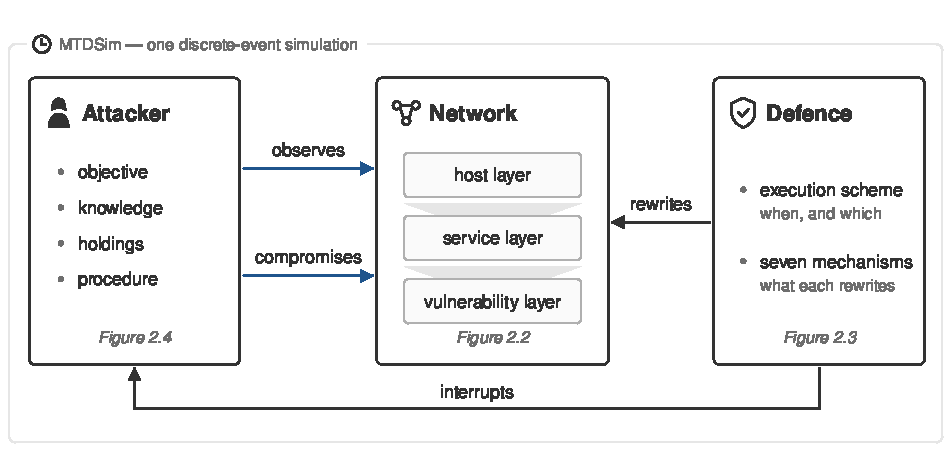
\includegraphics{fig_2-2a_mtdsim_model}
  \caption[The three modules of MTDSim]{The three modules of MTDSim and how
  each acts on the others.}
  \label{fig:mtdsim-model}
\end{figure}

MTDSim simulates an attacker and MTD on one network, to evaluate MTD
mechanisms singly and in combination \citep{brown2023}. Every attack action and
every deployment takes simulated time, counted in seconds \citep{zhang2023}.
Figure~\ref{fig:mtdsim-model} draws the simulator's three modules: the
attacker, the network and MTD. MTD deploys its mechanisms at intervals, and each
deployment reconfigures part of the network and disrupts the attacker. The
attacker observes part of the network and compromises hosts in it.
Section~\ref{subsec:network-model} describes the network's hosts, services
and vulnerabilities, Section~\ref{subsec:defence-mechanisms} the MTD
mechanisms and deployment strategies, and
Section~\ref{subsec:attacker-model} the baseline attacker.

% 2.2.1: Marc: "poorly drafted ... figures breaking up the text"; Figure
% 2.2 "visually bombarding ... trying to do too much". Kept: what ch4-ch5
% use (the two layers the mechanisms rewrite, levels, endpoints, the
% defaults, the target hosts, CVSS complexity, impact). Cut as used nowhere
% later: Barabasi-Albert, scale-free, Watts-Strogatz (which also described
% the seed, not the built service graph: host.py:545-590), the vulnerability
% layer's name, the internal target node, synthetic vulnerabilities. CVSS
% and impact defined here, at first use (ch3 l.~3930 defined them after ch2
% used them). The visible subgraph moved to 2.2.3, where the attacker uses
% it. Subnet defined (Marc did not follow it). Endpoint fact kept once and
% made exact: complete topology shuffle does move endpoint links
% (mtd_write_surfaces.md (a)).
\subsection{Network model}
\label{subsec:network-model}

\begin{figure}[t]
  \centering
  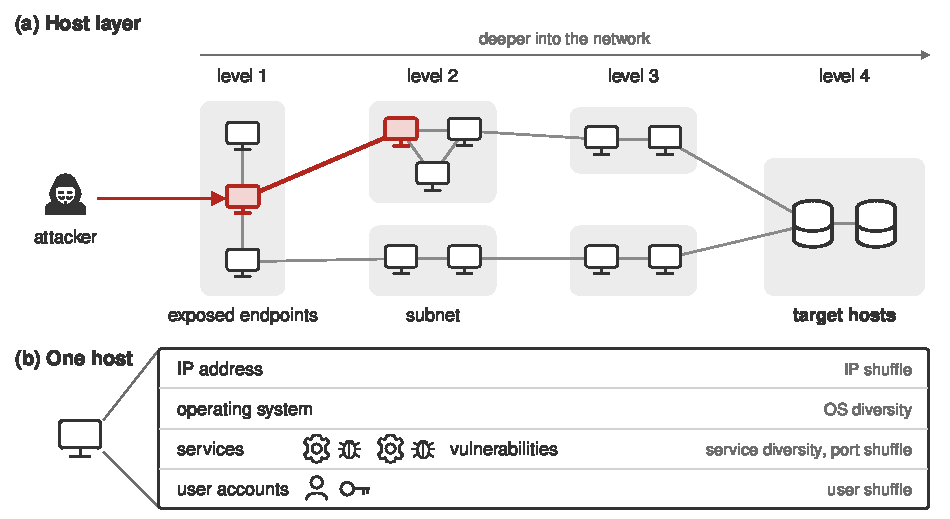
\includegraphics{fig_2-2-1a_network_model}
  \caption[The network, and one host in it]{The network, and one host in
  it. (a) The attacker enters at the exposed endpoints and works deeper,
  level by level, towards the target hosts; red marks its route and the
  hosts it has compromised. (b) What a host holds, and the MTD mechanism that
  reconfigures each part.}
  \label{fig:network-model}
\end{figure}

The network in MTDSim is a three-layer hierarchical attack representation
model (HARM) \citep{hongkim2012harm}: a graph of hosts, in which each host
runs services and each service carries vulnerabilities
(Figure~\ref{fig:network-model}). The \emph{host layer} is the topology:
the hosts are nodes, and an edge joins two hosts that can reach each other.
The \emph{service layer} is the services running on each host.

The hosts sit in levels of depth. The first level is the \emph{exposed
endpoints}, the hosts reachable from outside the network. Each deeper level
is a set of subnets, small groups of densely linked hosts, joined to the
level before it, so reaching a level requires a compromised host in the
level before it \citep{brown2023}. By default the network has 50 hosts in
four levels of depth and eight subnets, with five exposed endpoints. Five
database hosts at the deepest level are the \emph{target hosts} of the
targeted attack scenario (Section~\ref{subsec:attacker-model}). Every host
other than an endpoint is an \emph{internal host}.

Each host has an IP address, user accounts, one operating system and a few
services, each running on a port. The exposed endpoints keep their
address, software and accounts throughout: no MTD mechanism changes them,
although a topology shuffle can change their links. Each vulnerability has an attack complexity from the Common
Vulnerability Scoring System (CVSS), which sets the probability that an
exploit succeeds, and an \emph{impact}, the damage a successful exploit
does \citep{brown2023}. A service is compromised when the impact of its
exploited vulnerabilities passes a threshold, and a compromised service can
compromise its host.

% 2.2.2: heading now names both halves (ruling S1; the 5.3.3 heading's
% words). Marc: "missing your first sentence"; "attacker effect doesn't
% appear in Table 2.3"; shuffle/diversity "redefined". Now: what MTDSim
% deploys, grouped as Table 2.3 groups it. Cut as used nowhere later or
% duplicated: the optimised OS assignment withdrawal (a ruling of this
% dissertation, D-17(c), not background), the endpoint repeat, the 38 agents
% (Appendix E carries them), the same-layer concurrency rule, the duration
% provenance (Table 5.1 cites each value), the simultaneous deployment
% strategy (not run; Marc: "we could drop it"). "No detection channel is
% encoded" CORRECTED: MTDShield is told the attacker's current phase at its
% detection rate (mtd_ai_operation.py:557-566; Appendix E), and decides at a
% fixed tick with a forced deployment after 2 000 s, which is Cho's hybrid.
% "Deployment interval" defined (the ratified term; Table 5.1 points here for
% "near-periodic").
\subsection{MTD mechanisms and deployment strategies}
\label{subsec:defence-mechanisms}

MTDSim deploys seven MTD mechanisms: five shuffles, two diversities, and no
redundancy (Table~\ref{tab:defence-mechanisms}). Each reconfigures one part
of the network: the host layer, the service layer or the users' credentials.
A \emph{deployment} is one run of one mechanism, and takes from 20\,s to
110\,s to complete, depending on the mechanism \citep{zhang2023}.

\begin{table}[t]
  \centering
  \caption[The seven MTD mechanisms]{The seven MTD mechanisms, from the
  pool of Brown~\citep{brown2023}, added to by Zhang~\citep{zhang2023}, by
  the part of the network each reconfigures.}
  \label{tab:defence-mechanisms}
  % SDR class column CUT 2026-10-01 (Marc: "is SDR class column needed if
  % shuffle and diversity are in the name?"): each name ends in its class and
  % the prose counts them (five shuffles, two diversities, no redundancy), so
  % literature_conventions c3 is met by the names.
  \tablestyle
  \begin{tabular}{@{}P{4.4cm}P{11.0cm}@{}}
    \toprule
    Mechanism & What it reconfigures \\
    \midrule
    \grouprow{2}{Host layer} \\
    \quad IP shuffle & the IP address of every internal host \\
    \quad Complete topology shuffle & every connection between hosts, regenerated \\
    \quad Host topology shuffle & the positions of internal hosts, swapped in pairs within a level \\
    \addlinespace
    \grouprow{2}{Service layer} \\
    \quad OS diversity & the operating system of every internal host, and each service the new one cannot run \\
    \quad Service diversity & every service on every internal host, redrawn from those its operating system can run \\
    \quad Port shuffle & the port of every service on every internal host \\
    \addlinespace
    \grouprow{2}{Credentials} \\
    \quad User shuffle & the user accounts of every internal host, redrawn from the network's pool \\
    \bottomrule
  \end{tabular}
\end{table}

A \emph{deployment strategy} decides which mechanism is deployed, and when
(Table~\ref{tab:deployment-strategies}). The random, alternative and single
deployment strategies follow a schedule, so they are proactive
\citep{zhang2023}. MTDShield is a reinforcement-learning agent
\citep{tay2024}. At each interval it reads the network's security metrics
and the attacker's current attack action, and deploys one of four mechanisms
(complete topology shuffle, IP shuffle, OS diversity or service diversity)
or none; if 2\,000\,s pass without a deployment, one is forced. It adapts its
schedule to what it observes within a bound, so it is hybrid. No deployment
strategy is reactive.

The \emph{deployment interval} is the time between deployments: 200\,s by
default, and near-periodic \citep{tay2024code}.

\begin{table}[t]
  \centering
  \caption[The four deployment strategies]{The four deployment strategies:
  three from Zhang~\citep{zhang2023} and MTDShield, the
  reinforcement-learning agent of Tay~\citep{tay2024}.}
  \label{tab:deployment-strategies}
  \tablestyle
  \begin{tabular}{@{}llP{0.62\textwidth}@{}}
    \toprule
    Deployment strategy & Trigger & What it deploys at each interval \\
    \midrule
    random & proactive & a mechanism drawn at random \\
    alternative & proactive & the next mechanism in a fixed rotation \\
    single & proactive & the same mechanism every time \\
    MTDShield & hybrid & the mechanism its agent chooses, or none \\
    \bottomrule
  \end{tabular}
\end{table}

% 2.2.3: heading "Baseline attacker" (ruling S2). Marc: "every attacker is
% identical and uniform in skill ... not a fair presentation" --- the
% attacker is now described by what it does. One name for the six: "attack
% action", defined here (Marc, 2026-10-01: "attack actions ... makes the most
% sense in Figure 4.1 rather than a vague phases"; Zhang 2023's word, and
% Brown's metric "attack actions blocked"). Overturns the 2026-09-30 "phase"
% and its binding sentence; full term everywhere, ch1 to the appendices
% (registry row "The six inherited operations"). Kept: the fixed order (ch5
% l.~7236), the fallback order (ch3 l.~3926), return on attack (defined here,
% at first use), Zhang's halving (ch3 l.~3921, ch4 l.~5605), the visible
% subgraph (moved from 2.2.1), persistence (Table B.5). ADDED (the
% placeholder, owed for 5.3.1 and ch4 l.~5250): the confusion penalty
% (constants.py:147, 20 s; zhang2023 Sec. 4.4.3), the three interruption
% classes in the host-layer / service-layer / credentials vocabulary of
% Table 2.3 (attack_operation.py apply_mtd_interrupt_cost / _handle_interrupt;
% mtd_operation.py _interrupt_adversary), and what a deployment leaves the
% attacker (the old Figure 2.4 upper panel, now prose). Cut as used nowhere
% later: "uniform in skill", the ATT&CK half of the attribution (taught in
% 3.1.2), "ten enumerations", the procedure walk that repeated Table 2.5.
% Table 2.6 KEPT (Marc: "nice and brief").
\subsection{Baseline attacker}
\label{subsec:attacker-model}

\begin{figure}[t]
  \centering
  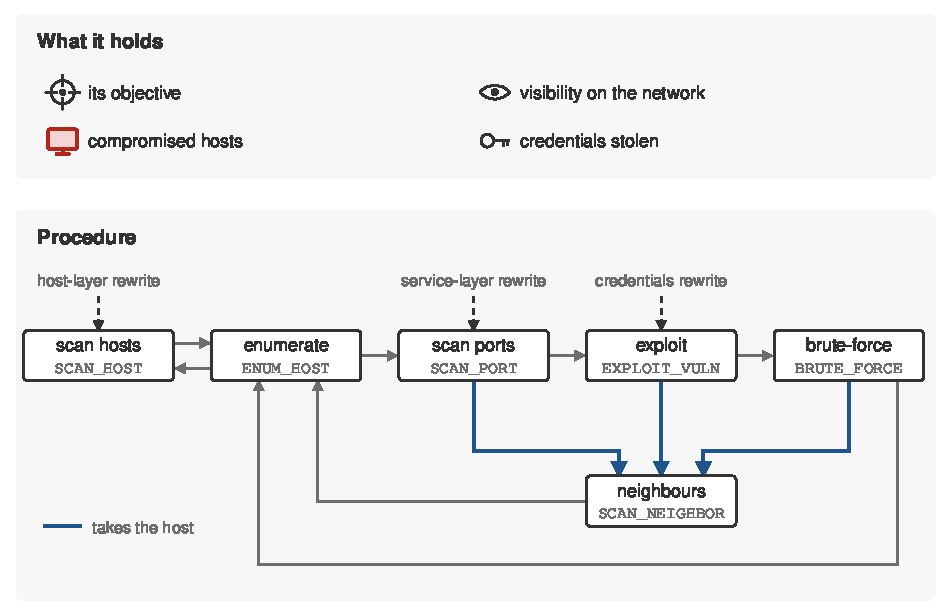
\includegraphics{fig_2-2-3a_attacker_model}
  \caption[The six attack actions of the baseline attacker]{The six attack actions of the
  baseline attacker and the moves between them. A dashed arrow marks the
  attack action each kind of deployment sends the attacker back to.}
  \label{fig:attacker-model}
\end{figure}

The baseline attacker is the attacker MTDSim was built with
\citep{brown2023}. It follows a fixed procedure of six \emph{attack actions}, modelled on
the Cyber Kill Chain \citep{brown2023, hutchins2011}: it scans for hosts,
enumerates one, scans its ports, exploits its vulnerabilities, brute-forces
its accounts, and scans the neighbours of each host it compromises
(Figure~\ref{fig:attacker-model}). The
attacker follows one of two attack scenarios
(Table~\ref{tab:attacker-objectives}).
% 2026-10-01 (Marc: the general scenario "has emphasis on compromising as
% much of the hosts as possible"; Zhang's 80 % is a variant, and "general
% scenario's stop" was "vague and forced"). The scenario is defined by its goal
% (Table 2.3); how a run ends is one sentence, no coined name. The reader needs
% only the thesis's ending rules (4.5, Table 5.1): each study's own ending is
% Table 2.4's "End of run" row. The 80 % ends a run in either scenario
% (attack_operation.py:743, checked before the target). SESSION-DRAFTED ---
% ratify on read.
A run ends when the attacker compromises more than 80\,\% of the hosts
\citep{zhang2023}, compromises a target host in the targeted scenario, or can
discover no new host.

\begin{table}[t]
  \centering
  \caption[The two attack scenarios of the baseline attacker]{The two
  attack scenarios of the baseline attacker \citep{brown2023}, by the
  attacker's goal.}
  \label{tab:attacker-objectives}
  \tablestyle
  \begin{tabular}{@{}ll@{}}
    \toprule
    Attack scenario & Goal \\
    \midrule
    General & compromise as many hosts as possible \\
    Targeted & compromise a target host \\
    \bottomrule
  \end{tabular}
\end{table}

The attacker knows only its \emph{visible subgraph}: the exposed
endpoints, the hosts it has compromised and their neighbours. On each host
it tries stolen credentials first, then exploits the vulnerabilities in
order of \emph{return on attack}, an exploit's probability of success times
its impact, divided by the time it takes \citep{brown2023}, and brute force
last.
% [DRAFT STATE 2026-10-05, from the 4.4.2 round-4 review (Marc: should
%  MTDSim's attack-action times be in the background, where the attack
%  actions are introduced, so the method can use them). Verified against
%  mtdnetwork/data/constants.py ATTACK_DURATION and
%  component/services.py Vulnerability.exploit_time; the x2.5 OS-mismatch
%  factor left off the page.]
Scanning for hosts, enumerating a host and scanning a host's neighbours
each take 5\,s, scanning its ports 25\,s and brute force
20\,s~\citep{tay2024code}. An exploit takes 15\,s times one minus the
vulnerability's attack complexity, which lies between 0.4 and
1~\citep{brown2023}, so from 0 to 9\,s. An exploit of a vulnerability it
has exploited before takes half the time \citep{zhang2023}.

% [TERM SWEEP 2026-09-30, Marc: "disrupt, 100 %, everywhere"] interrupt -> disrupt in own-voice prose, ch2/ch4/ch5 and Figures 2.1, 4.1; code names keep interrupt. Registry row re-affirmed.
A host-layer deployment disrupts the attacker
during any attack action and sends it back to scanning hosts, because the host it
was on may have moved. A service-layer deployment disrupts it only while
it scans ports, exploits or brute-forces, and sends it back to scanning the
same host's ports \citep{brown2023}. A user shuffle disrupts only brute
force, and sends it to exploit instead. Each disruption costs the
attacker a confusion penalty of about 20\,s \citep{zhang2023}. A deployment never
takes back a compromised host or a stolen credential \citep{zhang2023}; the
attacker loses only its place, and a topology shuffle also rebuilds its
visible subgraph.

The earlier MTDSim studies ran these three modules in the configurations
of Table~\ref{tab:lineage-configurations}.

% Table 2.2 --- GENERATED (tools/ch2_lineage_configurations_table.py from
% data/misc/lineage_configurations.yaml; one locator per cell in the
% fragment's header). Register E5, 2026-09-23. Rows are Table 5.1's
% parameters in Table 5.1's order, so the two read side by side. Moved
% 2026-09-30 from the 2.2 preamble to here, after every term in it is
% defined; Brown's interval converted from ms to s.
% GENERATED by tools/ch2_lineage_configurations_table.py from
% data/misc/lineage_configurations.yaml --- edit the YAML, not this file.
% Locators, one per cell (the caption's claims are checkable against these):
%   Hosts / Brown: 200  [Table I, p.5]
%   Hosts / Zhang: 25; 50; 75; 100  [Table 2, p.33 ("four networks with different sizes, ranging from 25 to 100 nodes")]
%   Hosts / Ho: 150  [Table 2 "Simulator Settings", p.19 (Total Nodes 150; held fixed while Ho's "network size" varies, p.19)]
%   Levels of depth / Brown: 5  [Table I, p.5 ("No. of layers"; levels of depth per p.2)]
%   Levels of depth / Zhang: 4  [Table 2, p.33 ("Layers", 4 on every network)]
%   Levels of depth / Ho: ---  [not stated (ho2024.md §B)]
%   Subnets / Brown: 20  [Table I, p.5]
%   Subnets / Zhang: ---  [not stated; Table 2 carries no subnet column]
%   Subnets / Ho: ---  [not stated (ho2024.md §B)]
%   Exposed endpoints / Brown: 20  [Table I, p.5 ("No. of exposed hosts")]
%   Exposed endpoints / Zhang: 3; 5; 7; 10  [Table 2, p.33 ("Endpoints", one per network)]
%   Exposed endpoints / Ho: ---  [not stated (ho2024.md §B)]
%   Attack scenario / Brown: general; targeted, a database host  [III.C.1, p.4 (Scenario 1; Scenario 2, "a specific 'target' host (e.g., a credential database)"); target at level 3 or 4, figure captions p.6]
%   Attack scenario / Zhang: general  [§4.4.1.1, p.28 (only the first scenario refactored)]
%   Attack scenario / Ho: general  [§3.1, p.15 ("to try to compromise as many hosts as possible")]
%   Deployment interval / Brown: uniform on 1\,000--5\,000\,ms  [Table I, p.5; §IV, p.5 ("E(T) = 3000 (time in milliseconds)")]
%   Deployment interval / Zhang: exponential, mean 50; 100; 150; 200\,s  [p.33 ("four MTD Intervals, ranging from 50 to 200 seconds"); levels from the Figure 8 panel titles, p.35; exponential, §4.3.4, p.27]
%   Deployment interval / Ho: 50; 100; 200  [Table 6, p.23 (no unit given); comparison with the execution schemes at 200, Table 8, p.24]
%   Deployment duration / Brown: ---  [not stated (provenance.md, IS-TIM-03)]
%   Deployment duration / Zhang: complete topology shuffle 110\,s, IP shuffle 100\,s, OS diversity 80\,s, optimised OS assignment 80\,s, service diversity 70\,s  [Table 3 "MTD Execution Time", p.34 (standard deviation 0.5 on each)]
%   Deployment duration / Ho: ---  [not stated (ho2024.md §B)]
%   Run ends / Brown: attack goal met  [III.C.1, p.4; no time limit stated (brown2023.md §B)]
%   Run ends / Zhang: 80\,\% of hosts compromised  [p.33 ("the terminating condition for the simulation as the NCR reaching 0.8")]
%   Run ends / Ho: 15\,000  [Table 2, p.19 (Finish Time 15000; no unit given)]
%   Runs per combination / Brown: ---  [not stated (brown2023.md §B)]
%   Runs per combination / Zhang: 100  [p.33 ("run the simulation 100 times for each variable set")]
%   Runs per combination / Ho: ---  [not stated; the 100 of Table 1 is training episodes, not evaluation runs (ho2024.md §B)]
\begin{table}[htbp]
  \centering
  \caption[The configurations of the MTDSim lineage]{The configurations the studies of the MTDSim lineage evaluated on. Values separated by semicolons were each run; a dash marks a value the study does not state. Ho gives the interval and the run's end without a unit; the simulator Ho ran counts in seconds \citep{zhang2023}. Tay \citep{tay2024} states no network, timing or run value.}
  \label{tab:lineage-configurations}
  \tablestyle
  \begin{tabular}{@{}P{3.0cm}P{3.7cm}P{4.6cm}P{3.4cm}@{}}
    \toprule
    Parameter & Brown \citep{brown2023} & Zhang \citep{zhang2023} & Ho \citep{ho2024} \\
    \midrule
    Hosts & 200 & 25; 50; 75; 100 & 150 \\
    Levels of depth & 5 & 4 & --- \\
    Subnets & 20 & --- & --- \\
    Exposed endpoints & 20 & 3; 5; 7; 10 & --- \\
    Attack scenario & general; targeted, a database host & general & general \\
    Deployment interval & uniform on 1\,000--5\,000\,ms & exponential, mean 50; 100; 150; 200\,s & 50; 100; 200 \\
    Deployment duration & --- & complete topology shuffle 110\,s, IP shuffle 100\,s, OS diversity 80\,s, optimised OS assignment 80\,s, service diversity 70\,s & --- \\
    Run ends & attack goal met & 80\,\% of hosts compromised & 15\,000 \\
    Runs per combination & --- & 100 & --- \\
    \bottomrule
  \end{tabular}
\end{table}


% Chapter close, ratified 2026-09-26; "scripted" cut (the section no longer
% calls it that). 2026-09-30 (Marc: the specific version "lost sight of its
% purpose"): the hand-over only --- the baseline just described is set beside
% an APT attacker next; the eight properties are ch3's to introduce.
% LAYOUT PIN (2026-10-01, Marc): the page break sets Tables 2.3 and 2.4 at
% the top of the next page with this sentence beneath them, instead of on a
% float page of their own after it. Re-check if text above it changes.
\newpage
Chapter~\ref{ch:litreview} compares the baseline attacker, and the attacker
models of recent MTD evaluations, with an APT attacker.


% =====================================================================
\chapter{Literature review}
\label{ch:litreview}

% DRAFT STATE (2026-08-31): PATCHWORK FIRST DRAFT, assembled from the
% submitted review's own audited sentences (port ledger, sentence by
% sentence: docs/handoffs/2026-08-31_ch3_patchwork_draft.md; shape and
% CONFIRMs: docs/handoffs/2026-08-31_ch3_port_plan.md). Inserted on
% Marc's instruction; the four batch conversions ([D2] em-dashes, [T]
% adversary -> attacker, [FP] forward pointers cut, [PoP] pyramid cut)
% and the seven [stitch] sentences are applied as recommended, each
% reversible per item. Gaps G0--G8 are visible placeholders for Marc's
% dictation. Order ratified 2026-08-31: capture -> evaluate -> model,
% the model strand closing on the fidelity gap (port plan CONFIRM 1);
% the eight axes are derived here and adopted in sec:requirements
% (CONFIRM 2 --- the sec:movement-attacker preamble's axes \ref still
% points at sec:requirements; re-point once sec:requirements is folded).
% [2026-09-04] EXECUTED past CONFIRM 2: §4.1 is cut, not folded; the ch4
% preamble's \ref now points at subsec:attacker-criterion.
% Ledger: 3 000 words / 12 units = preamble 1 / 3.1 3 / 3.2 3 / 3.3 5;
% assembled text ~3 450 excluding gaps, pass 5 reconciles across the
% section. Headings ruled 2026-08-31 (sharp noun phrases; ATT&CK treated
% as a proper name). STRUCTURE AMENDED 2026-09-02 (Marc's ruling, no
% unit added or deleted): 3.2 reordered to opener (anatomy sentence,
% unnumbered) -> Metrics -> Evaluation methods (renamed from
% "Validation methods"; Cho's own Sec. VIII title) -> the hinge as an
% unnumbered strand closer (was 3.2.3 "Metrics and the attacker
% model"); 3.3 subsections swapped to traditions -> criterion (survey
% -> instrument -> measurement -> verdict). Ruling trail:
% docs/handoffs/2026-08-31_ch3_patchwork_draft.md (amendment note).
% STRUCTURE AMENDED 2026-09-05 (Marc's ruling, design session then
% item-by-item approval; branch feat/ch3-evaluation-anatomy). 3.2 now
% carries Cho's anatomy in full: opener (anatomy in the registry's
% terms; network model + defence mechanisms dispatched to ch2; the
% attacker model to 3.3) -> 3.2.1 Defence modelling approaches (NEW
% heading, Cho Sec. VI; the traditions paragraph moved here, G4b
% re-homed as its P2) -> 3.2.2 Metrics (the "mode of modelling" [3b]
% resolved to the registry term; the scored-over pivot parked at its
% P2 tail as G1a --- RETIRED 2026-09-07, one dictated sentence in its
% place) -> 3.2.3 Evaluation methods (G4a re-homed, fused
% with G6) -> closer (G1 trimmed to the synthesis). 3.3: "Attacker
% modelling traditions" DELETED as a heading (Bland/Outkin -> the
% gap); the interstitial cut to the move; the diagnosis stated ONCE,
% in the criterion; "Threat models in recent MTD evaluations" ->
% "Attacker models in recent MTD evaluations"; "The research gap" ->
% "Research gap". threat model -> attacker model thesis-wide in own
% voice (terminology.md row RATIFIED 2026-09-05). Ledger: 11 units =
% preamble 1 / 3.1 3 / 3.2 3 / 3.3 4, one unit of slack returned.
% Guardrail carried on 3.2.1 (Marc's trap): it names where the FIELD's
% attacker comes from and never says "this thesis uses none of these".
% Bib (2026-08-31): every key this chapter cites is
% active in references.bib (eleven uncommented, ho2024 added). NIST SP
% 800-39 (G7a) ACTIVATED 2026-09-02, verified against the PDF; the Volt
% Typhoon advisory AA24-038A (G5) was ACTIVATED 2026-08-31 --- both
% await Marc's sighting. \ref{tab:lineage} assumes ch2's Table 2.1 label.

% Preamble (unnumbered, 1 unit). RECAST 2026-09-08 on Marc's ask ("what
% does this need to carry --- a narrative thread, then prescriptive:
% what each section does, and that it motivates chapter 4"; the
% "two literatures" flourish is "on repeat"). Design record: port plan
% §2 preamble row (the scissors; strands keyed to the sub-questions;
% the selection rule; the coverage claim planted) and §5 refusals (no
% RQ restatement; no "the remainder is structured as follows").
% CARRIES: S1 the thread (the scissors in one sentence: two literatures
% and the hinge between them); S2 the three strands keyed to SQ1--SQ3
% by \ref, in the chapter's order, with the one-clause reason the order
% differs from the sub-questions' (the model strand closes on the gap);
% S3 the selection rule, stated once for the chapter; S4 the coverage
% claim (a narrative review of three strands, not a systematic one); S5
% the close into ch4. CUT, SUPERSEDED for the record: P1 "Two
% literatures have developed alongside one another without converging.
% On the defence side, MTD evaluation has progressed from fixed-interval
% mechanisms toward adaptive, increasingly learned orchestration of
% when and what to move \citep{cho2020}. In parallel, the
% threat-intelligence community has built an apparatus around attacker
% behaviour: MITRE ATT\&CK established a behavioural vocabulary in 2013
% \citep{strom2018mitre}, and the structured extraction of that
% behaviour from cyber threat intelligence (CTI) has advanced rapidly
% since 2022 \citep{ctid2025attackflow}." (3.1.2 carries ATT&CK's origin
% and Attack Flow; 3.2 carries the orchestration progression) and the
% signature line "The defender has grown more sophisticated; the
% attacker against which it is evaluated has not." (a verdict before
% the measurement --- voice §c9; 3.3.3 now carries the verdict in Marc's
% words; revivable as the chapter's one vivid line on his word); P2
% "The capability to close this gap already exists in literatures
% adjacent to MTD, but has not been adopted within it. Attack profiling
% reconstructs attacker behaviour from CTI as structured
% representations at the level of tactics, techniques, and procedures
% (TTPs) \citep{rodriguez2024}, and the documented durability of
% advanced persistent threat (APT) tradecraft makes such profiles a
% stable basis for evaluation \citep{alshamrani2019}." (3.3.3 P2 is the
% means paragraph; 3.1.2 the durability argument; "close this gap"
% names the gap before the chapter derives it). G0 RETIRED into S1--S4.
% RECAST AGAIN 2026-09-09 (Marc: "two literatures" reads as a framing
% a general CS reader will not follow; frame it as MTD against APT
% attackers --- captured, modelled, evaluated, the sub-questions; the
% selection-rule and coverage-claim sentences not understood). Brought
% to the ch2 preamble's register (two sentences, plain, by pointer).
% S3/S4 (selection rule, coverage claim) CUT: the selection rule lives
% where a sample is drawn (3.3.2 P1); the coverage claim (narrative,
% not systematic) is parked in the handoff §13 as an examiner-facing
% sentence to add only if asked. SUPERSEDED 2026-09-08 draft: "Two
% literatures bear on the evaluation of MTD against an APT attacker:
% the record of how APT campaigns behave, and the instruments by which
% a defence is evaluated; between them sits the attacker model the
% instruments are scored over. The chapter surveys the three in turn.
% ..." Connective prose, session-drafted under the green light; RATIFY
% ON READ. DRAFT STATE (2026-09-09).
% [CONNECTIVE-PROSE PASS 2026-09-26, P6 ch3 opener] The three section
%  clauses given what each section delivers (they were topics under one
%  verb); S1 and the 'last because' dependency unchanged.
%  SESSION-GENERATED on Marc's 2026-09-26 go-ahead
%  (docs/workflows/connective_prose.md; audit
%  docs/implementation/connective_prose_audit.md); prior text in git.
%  RATIFIED 2026-09-26 (Marc: 'I accept all this').
% [CH3 REDRAFT ROUND 2, 2026-10-01, O] Opener: link to the research question, aim, then the three sections by what each does. SESSION-DRAFTED on Marc's walk-through ("the narrative is a bit disjointed ... clarity and relevance"); ratify on read. Prior text in git.
% [CH3 REDRAFT ROUND 4, 2026-10-01, O] Marc: "locates" -> "identifies the research gap"; "enters" -> "how attacker models are used"; "draws" -> "surveys" (his literal verb). Ratify on read.
% [CH3 REDRAFT ROUND 3, 2026-10-01, O] Marc: the "but" read as a false dichotomy (as if an APT attacker cannot be modelled); the chapter's aim is the gap between MTD attacker models and APT attackers, which the literature supplies and the chapter re-derives. Link -> aim -> how (connective_prose.md (b)); says where the gap is drawn, not the gap (yardstick checklist 1). Ratify on read.
MTD is evaluated against attacker models, such as MTDSim's baseline
attacker (Chapter~\ref{ch:background}), and the research question asks how
it performs against APT attackers. This chapter identifies the research gap
between MTD attacker models and APT attackers. Section~\ref{sec:apt-survey} defines the
APT attacker and surveys how its behaviour is recovered from CTI
(\ref{sq:capture}). Section~\ref{sec:mtd-evaluation-survey} surveys how MTD
is evaluated and how attacker models are used in the evaluation
(\ref{sq:evaluate}). % [CH3 REDRAFT ROUND 47, 2026-10-02, ch3 intro] Marc ruled the logic fix ("well thought through and well integrated"): the unit asserted its conclusion as its premise (the APT definition says what an APT attacker is, not what MTD attacker models lack; the surveys' evidence covers six of the eight). The criterion section now says what an MTD attacker model needs; the lack is the surveys' finding for six and 3.3.2's for all eight. Ratify on read.
Section~\ref{sec:mtd-attacker-models} sets out eight properties an MTD
attacker model needs to model an APT attacker, and scores three recent MTD
attacker models on them (\ref{sq:model}). Section~\ref{subsec:research-gap}
% [CH3 REDRAFT ROUND 66, twin] 3.4 now points to Ch 4 and Ch 5; ratify on read.
states the research gap and how Chapters~\ref{ch:attacker-model}
and~\ref{ch:experiments} fill it.
% [CH3 REDRAFT ROUND 41, 2026-10-02, O] "scores recent MTD evaluations on those properties" -> "scores three recent MTD attacker models on them": Table 3.3 scores attacker models, and 3.3.2's heading now says so (one term). Ratify on read.
% [CH3 REDRAFT ROUND 8, 2026-10-01, O] Marc: "them" unclear, the 3.4 clause too verbose. "missing from MTD attacker models" (3.3.1 carries the literature as source); "scores ... on those properties" (Table 3.3's own verb). Ratify on read.
% [CH3 REDRAFT ROUND 7, 2026-10-01, O + S5] Marc: the eight properties are not a definition of the APT attacker (that is 3.1.1's) but the subset MTD attacker models are said to lack; "compares", not "survey" (two works and the lineage); the research gap promoted from 3.3.3 to its own section 3.4, the chapter-level close drawn from all three strands (yardstick (c)3). Ratify on read.
% [CH3 REDRAFT ROUND 6, 2026-10-01, O] Marc: the gap was named twice (aim and last sentence). The aim sentence now carries the gap and the hand-over to Chapter 4; the Section 3.3 sentence states what the section does (criteria from the literature, then scoring), the conventional scored-review order (yardstick (c)4; Bonneau et al. 2012). Ratify on read.
% [CH3 REDRAFT ROUND 5, 2026-10-01, O] last sentence: three clauses to two, the colon equating what recent evaluations still lack with the research gap (Marc: "clunky"). Was "..., checks whether recent MTD evaluations still lack it, and states the research gap that motivates Chapter 4". Ratify on read.

% ------------------------------------------------------- 3.1 capture --
% Feeds capture: can the literature hand you a machine-usable
% behavioural specification of a campaign, and what does it still not
% carry. 3 units.
% [CH3 SCRUTINY 2026-09-30, S1] heading was "Survey of APT attackers"; now the opener's words.
\section{APT attacker behaviour}
\label{sec:apt-survey}

% [3.1 INTERSTITIAL --- RULED 2026-09-04 (Marc). SESSION-GENERATED
% connective prose under the standing green light (common thread +
% each subsection as is; no content): the strand's question (the port
% plan's own framing of 3.1) in one sentence, then functional
% signposting whose nouns are each subsection's own claim-sentence
% nouns (APT attacker / lifecycle; knowledge base; structured
% representations). Framing evolved through four rounds in chat: the
% two orphan sentences from the 3.1.1 dissolve (S1 "well-documented"
% --- uncited; S5 the commodity/multi-step-commitment contrast) are
% CUT in full --- the commodity-attacker thread is dead everywhere
% else in the chapter (E1, 3.1.1), so it is not carried here either.
% Marc's rulings, do not re-flag: "surveys" not "asks"/"looks at"
% (the heading's own verb); "machine-usable" not "machine-readable"
% (STIX is already readable; usable is the gap); "current limitations"
% not "the two gaps that remain" (the 3.1.3 exit's declarative is
% itself booked for his rework); no "lingua franca" echo (a cited claim,
% not a signpost); no sub-question keying (G0's job). Pass 6 run
% 2026-09-04: no proposals; §(f) gate passes all nine.]
% [CH3 REDRAFT ROUND 2, 2026-10-01, 3.1 preamble] The section's question in one sentence (recover, SQ1's verb), then each subsection by what it does. SESSION-DRAFTED on Marc's walk-through ("the narrative is a bit disjointed ... clarity and relevance"); ratify on read. Prior text in git.
% [CH3 REDRAFT ROUND 9, 2026-10-01, 3.1 preamble] Marc: "modelled only from what is recorded" jumped to modelling; the section is about recovering the behaviour of real attackers (SQ1's words), and "what it still cannot recover" was vague. Frame = how and how far; each subsection hands the next its open question: which techniques (ATT&CK) -> in what order (profiling) -> not the tempo (the 3.1.3 exit's term). Ratify on read.
% [CH3 REDRAFT ROUND 10, 2026-10-01, 3.1 preamble] Marc: the nuance weighs in; say only what the reader needs. The limits ("how far", "not in what order", "not the tempo") are cut: the 3.1.3 sentences state them where they are argued. Ratify on read.
This section surveys how the behaviour of APT attackers is recovered from
CTI. Section~\ref{subsec:apt} defines the APT attacker.
Section~\ref{subsec:attack} describes MITRE ATT\&CK, the knowledge base
that records attacker behaviour as techniques.
Section~\ref{subsec:profiling} describes attack profiling, which recovers
the order of an attack's techniques from CTI.
% [CONNECTIVE-PROSE PASS 2026-09-26, T1 3.1 preamble] 3.1.3's heading term
%  named in the preview. SESSION-GENERATED on Marc's 2026-09-26 go-ahead
%  (docs/workflows/connective_prose.md; audit
%  docs/implementation/connective_prose_audit.md); prior text in git.
%  RATIFIED 2026-09-26 (Marc: 'I accept all this').

% 1 unit. Review Sec. III-C, tightened. [Flag resolved 2026-09-02, Marc's
% ruling: the third paragraph is DISSOLVED --- S1+S5 up to the 3.1
% interstitial, S2's salvage clause and S3 into 3.1.2, S4 to open 3.1.3,
% the duplicated halves of S2/S3 cut. Subsection shape is now
% definition -> lifecycle -> G5 current reporting.]
\subsection{Advanced persistent threat}
\label{subsec:apt}

% [CH3 REDRAFT ROUND 11, 2026-10-01, 3.1.1] Marc approved the restructure: two paragraphs, what an APT attacker is, then how its operation unfolds. One definition (was three overlapping: Alshamrani, the three-term gloss, NIST's restatement), each property said once in Table 3.2's words (persistent, adapts, stealth, objective) so 3.3.1's pointer lands; NIST expanded at first use and named, so 3.3.1's "the NIST definition (Section 3.1.1)" still resolves; "low and slow" kept (ch4's low-and-slow family rests on it); the M-Trends evidence moved beside the stealth claim; "retooling at a tempo" cut (adapts carries it), and with it the tempo/pacing drift. Content reused, no new claims. Round 12: "The name gives its three properties" -> "Each word of the name stands for one property" (Marc: not specific). Ratify on read. Prior text in git.
An APT attacker is a well-resourced attacker, typically sponsored by a
nation-state or organisation, that pursues a specific objective against a
specific target \citep{alshamrani2019}. Each word of the name stands for
one property. It is \emph{advanced} in its tooling and tradecraft
\citep{alshamrani2019}. It is \emph{persistent}: in the definition of the
US National Institute of Standards and Technology (NIST), it pursues its
objective repeatedly over an extended period and adapts to the defender's
resistance \citep{nist2011sp80039}. It moves low and slow, trading speed
for stealth \citep{alshamrani2019}: espionage intrusions go undetected for
a median of 122 days, against 14 days across all intrusions
\citep{mtrends2026}. And it is a \emph{threat} defined by its objective:
data exfiltration, impediment of mission-critical components, or
positioning for future operations \citep{alshamrani2019, nist2011sp80039}.
% [terminology ruled 2026-09-02: "APT actor" -> "APT attacker"
% (registry row ratified; Alshamrani's own phrase). "Volt Typhoon
% actors" below stays --- source-echo carve-out.]
% [G7a resolved 2026-09-02] direct cite of SP 800-39's APT definition
% (App. B, p. B-1): "(i) pursues its objectives repeatedly over an
% extended period of time; (ii) adapts to defenders' efforts to resist
% it; and (iii) is determined to maintain the level of interaction
% needed to execute its objectives". Paraphrase checked against the PDF
% Marc supplied; bib entry activated from its VERIFY stub, Marc to sight.
% [E1 CUT, ruled by Marc 2026-09-02 (pass 5 elastic): "This is
% precisely what the commodity attacker is not: single-run,
% smash-and-grab operations that neither hide nor adapt and end at
% first detection \citep{alshamrani2019}." TECHNICAL-CLAIM FLAG: the
% transience foil (single-run / non-adaptive / ends at detection) now
% has no prose home --- the 3.1 interstitial's commodity contrast is
% heterogeneity, a different axis; carrier is the alshamrani2019
% citation. E2 ruled same day: the espionage-contrast sentence KEEPS
% its pared (C7) form --- do not re-flag.]

% [CH3 3.1.1 P2 REDRAFT, 2026-10-04, Marc: the four stages are a synthesis of
%  the literature, so they belong here, not first in 4.4.4 ("we can't use
%  something that we haven't defined in the literature review"). One
%  lifecycle, not two: the four stages stated as OUR grouping (no source has
%  these four; Alshamrani's five are themselves a merge of Mandiant's seven and
%  Ussath's three; Che Mat finds the models vary "only slight[ly] in the
%  titles and the number of phases", extractions/chemat2024.md Table 4). Stage
%  names verbatim from the first sentence (Marc: prepare / foothold / operate /
%  act did not line up with them). Last stage "actions on objectives" (Marc's
%  ruling: "objective" is the attacker's objective, 4.2's classification key;
%  the Cyber Kill Chain's phase name, whose scope also holds lateral
%  movement). Foothold = what initial access gains (4.4.4's rule); intrusion =
%  foothold + running code (initial access + execution). Cut: Alshamrani's five
%  stage names (three are ATT&CK tactic names, met in 3.1.2), cleanup (only
%  Alshamrani has it; nothing downstream uses it), "performed discovery without
%  exfiltrating data" (a tactic name before 3.1.2; CISA reports credential
%  databases exfiltrated, not bulk data). Positioning stays in post-intrusion
%  operations: Alshamrani II-C (it "does not enter stages 4-5"); Volt Typhoon:
%  footholds for at least five years, pre-positioning to disrupt OT in a
%  future crisis (CISA, high confidence). The tactic-to-stage seating is ours
%  and stays in chapter 4 (lifecycle_consensus.md). Previous text in git.
%  DRAFT STATE, ratify on read.]
This dissertation groups the stages of published lifecycle models of an attack
\citep{hutchins2011, mandiant2013, alshamrani2019} into four: preparation,
intrusion, post-intrusion operations and actions on objectives. The models
differ in the names and number of their stages but follow a comparable
cycle \citep{chemat2024}. In preparation, the attacker researches its
target and builds its tools; in intrusion, it gains a foothold on a host in
the target's network and runs its code there; in post-intrusion operations,
it moves through the network undetected; in actions on objectives, it
steals data or impedes the victim's systems. Preparation and intrusion are
the same for every APT attacker; post-intrusion operations and actions on
objectives depend on its objective \citep{alshamrani2019}. An attacker
positioning for future operations stays in post-intrusion operations
\citep{alshamrani2019}. Volt Typhoon, for example, held footholds in US
critical infrastructure networks for at least five years, to disrupt their
operational technology in a future crisis \citep{cisaaa24038a}.

% [G5 DRAFT, dictated by Marc 2026-09-02; repaired (pass 2+3a),
% arranged to the scaffold order on his ask. 3b WALK DONE 2026-09-02
% ("all the 3b markers I accept"): every marker resolved in the
% direction it flagged, each ruling logged inline --- flip any by its
% log. PASS 4 RUN 2026-09-02; Marc RULED on 3.1.1 same day: M1a/M1b
% implemented as session-proposed wording (ratify-on-read, originals in
% their logs), M3b resolved by removing the Chapter~1 clause on the
% convention answer, the minor 3b resolved by naming M-Trends. Still
% open elsewhere in 3.1: [INSERT M2] (3.1.2), [TIGHTEN M3a] (3.1.3).
% PASS 5 RUN 2026-09-02, split-stream (WB+BB subagents), merged ledger;
% Marc blanket-ACCEPTED the convergent C-block (C1-C10, -56 w, applied
% across the whole subsection): triad dedup to the definitional site
% (S6 keeps only the forgo-exfiltration rider); "These reports..."
% sentence cut (supersedes, not reverses, its 3b noun ruling); S7
% trimmed to the currency clause; "For example," cut from the M1a
% sentence; "using capability and infrastructure" cut (colon-gloss
% carries it); the low-and-slow law-of-the-land flourish cut; espionage
% pads cut; S1's adaptation clause cut (attribution now rides on the
% NIST sentence); the custom-malware parenthetical cut (citation
% carries it); "recognisable" cut. E1 RULED same day: commodity foil
% CUT in full (claim flag at its site); E2 RULED: espionage-contrast
% sentence keeps its pared form. Unit ~267 w vs 250; residual ~17 to
% section assembly (2026-08-18 ruling). DO NOT RE-FLAG (pass-5 rejections):
% R1 the NIST behavioural sentence stays (G7a resolution); R2 the
% currency opener stays (claim-first); R3 "against a specific target"
% stays; R4 the sponsorship clause stays. PASS 6 RUN AND RULED
% 2026-09-02: P1-P4 accepted and applied (demonstrative run broken,
% NTDS.dit and OT defined at first use, advisory cite repeated at its
% run's end); gate now passes all nine checks. The APT-attacker/actor
% registry row remains PROPOSED (terminology.md) --- the NIST
% sentence's "an APT actor" awaits that ruling pass. §3.1.1 is THROUGH
% PASS 6; the integration check runs on the assembled 3.1 once 3.1.2 /
% 3.1.3 clear their passes (M2 / M3a still open there). Guardrails:
% the advisory is cited for what a documented campaign looks like and
% on what timescale, never as an MTD claim; no MTD mention here (that
% move is ch1's, notes/ch1_introduction/
% mtd_absent_from_volt_typhoon_response.md); do not imply the campaign
% is modelled (flow outside the corpus).]
% [CH3 SCRUTINY 2026-09-30, A3] P3 cut to the pacing claim and one objective contrast: the five years, LOTL, NTDS.dit and the espionage contrast are cut (ch1 P1 tells the first two; X7: "over a shorter time frame" is not in AA24-038A); "dwell time" leaves ch3 (it collided with ch4's dwell time, l.~4953). The comments below trail the cut sentences. Prior text in git.
% [CH3 REDRAFT ROUND 11, 2026-10-01, 3.1.1 P3] Paragraph dissolved: the M-Trends sentence moved to P1 (stealth), Volt Typhoon to P2 (objective). "The pacing depends on the objectives" CUT, which OVERTURNS the pass-4 KEEP below; its job is carried by "the last three depend on its objective". The comment trail below describes the old paragraph.
% [M1a IMPLEMENTED 2026-09-02, Marc's ruling ("propose a more nuanced,
% more accurate sentence") --- SESSION-PROPOSED WORDING, ratify-on-read.
% Carries the nuance: 14 d = all intrusions (eCrime-dominated
% population), 122 d = the espionage class. Also resolves the [3b]
% stage direction by naming M-Trends. Original dictated sentence: "For
% example, this CTI vendor report reports that APT attacks have a
% global median dwell time of 14 days and espionage-class intrusions
% 122 days". Grounding: breach_reports_macro_timing.md.]
% [M3b RESOLVED 2026-09-02, Marc's ruling on the convention answer
% (reviews do not justify an example by its use in the introduction;
% cross-references run intro -> chapter, not the reverse): the clause
% "The example that we bring up in Chapter~1," is REMOVED, minimal
% surgery, rest of the sentence untouched. The ch1 case study itself
% is unaffected (its note stands).]
% [KEEP --- pass 4] "The pacing depends on the objectives" is the
% unit's hinge: it is simultaneously M-Trends' own pacing-divergence
% framing (breach_reports_macro_timing.md) and Alshamrani's
% objective-conditioned suffix --- one sentence welds the statistical
% evidence to the definitional claim two paragraphs up.
% [3b ruled 2026-09-02, accepted: "may establish" -> "established"
% (the advisory reports observed fact).]
% [VERIFY watchlist] dictated "OT environment" repaired to "IT
% environments" --- the advisory's words are "within some victim IT
% environments" (OT is the target; IT is where the footholds sit).
% [pass 6 P2 applied 2026-09-02, accepted: NTDS.dit defined at first
% use by the advisory's own apposition ("the Active Directory
% database").]
% [3b ruled 2026-09-02, accepted: seam kept; "from three domain
% controllers" inserted per the marker (advisory fact, Overview of
% Activity).]
% [M1b IMPLEMENTED 2026-09-02, Marc's ruling --- SESSION-PROPOSED
% WORDING, ratify-on-read. Subject re-scoped from "APT attackers" to
% "Volt Typhoon actors" (the advisory's own term; the silence /
% discovery / re-validation facts are its observations of this
% campaign specifically, cisaaa24038a.md Concept 2). Two further
% repairs in the same move: "very silent" -> "largely silent" (the
% advisory reports "minimal activity"), and "and would perform" ->
% ", performing" to carry the re-scoped subject. Original dictated
% sentence: "... APT attackers were very silent after credential
% dumping and would perform discovery without bulk exfiltration,
% persistence maintained and revalidated".]
% [pass 6 P3 applied 2026-09-02, accepted: OT spelled at first use.]
% [3b ruled 2026-09-02, accepted: doubled halves cut to one --- the
% FIRST kept (carries "as an objective" and the future OT disruption);
% the cut half was "the agencies assess pre-positioning for OT
% disruption", whose attribution now rides on the citation and the
% next sentence. Flip if the agencies-attribution should be in prose.]
% [pass 6 P4 applied 2026-09-02, accepted: the advisory cite repeated
% at the end of its derived run (NTDS -> pre-positioning -> espionage
% contrast), closing gate check 3.]
% [3b ruled 2026-09-02, accepted: "impact" -> "exfiltration" (the
% advisory's contrast class is espionage/intelligence gathering, i.e.
% collection).]
% [3b ruled 2026-09-02, accepted: closing cite added.]
% [pass 6 P1 applied 2026-09-02, accepted: "This is" -> "Pre-positioning
% is" --- breaks the run of three demonstrative openers (voice SS d:
% pairs, never three) and anchors the referent; the remaining "That
% is... This is..." pair is the licensed two-beat.]
% [KEEP --- pass 4] the close pays off the lifecycle paragraph's "may
% forgo exfiltration entirely" with the live campaign --- faithful to
% both sources (nist2011sp80039 App. B; cisaaa24038a.md Concept 4),
% and it pre-loads the objective-conditioning story the model chapters
% need the literature to have told.

% 1 unit. Review Sec. III-A whole + Sec. III-B para 2 (Sadlek; pyramid
% cut). RESTRUCTURED 2026-09-02 (Marc's ruling): the argument inverted
% big-to-small --- P1 the knowledge base and its status, P2 the matrix
% and the hierarchy, with a matrix-derivation figure. The Attack Flow
% material (S3 clause + the serialisation-gap paragraph + Figure)
% moved to the bottom of 3.1.3 --- REVERSES the 2026-08-31 no-split
% ruling, Marc's own reversal: Attack Flow is now introduced with
% attack profiling, where the manual-curation exemplar uses it.
% Sentences are Marc's, rearranged; seams and gaps flagged, not
% written over.
\subsection{MITRE ATT\&CK}
\label{subsec:attack}

% [CH3 REDRAFT ROUND 2, 2026-10-01, 3.1.2 P1] Catalogue IDs cut (Marc: the brackets break the flow, and nothing comes back to them). SESSION-DRAFTED on Marc's walk-through ("the narrative is a bit disjointed ... clarity and relevance"); ratify on read. Prior text in git.
MITRE ATT\&CK is a knowledge base of attacker behaviour derived from
real-world observations, developed by the MITRE Corporation in 2013
\citep{strom2018mitre}, and the common language for attacker behaviour
\citep{ferraz2026, buchel2025}. It holds the attack matrix alongside
catalogues of named attacker groups and their campaigns,
each group characterised by the techniques observed across its operations
\citep{mitre2026attackkb, alsada2024}.
% [moved 2026-09-02 restructure: the lingua-franca sentence forward
% from mid-P2 --- the subsection's purpose sentence, now stated before
% the mechanics rather than after them.]
% [P1 reshape, Marc's 2026-09-02 feedback walk: purpose of P1 = what
% ATT&CK is + why it matters + what is in it. Order: knowledge base ->
% contents (matrix + catalogues, groups as a concept only) -> domain
% decomposition -> Enterprise richest. The earlier [GAP] (name the
% matrix) is filled by the merged contents sentence below.]
% [cite placement 2026-09-02 (Marc's ruling, citation review): the
% knowledge base vouches for the catalogue entries, Al-Sada for the
% characterisation claim.]
% [3b --- merge joint, flagged: "The knowledge base holds the attack
% matrix alongside catalogues of" replaces "Beyond the matrix itself,
% ATT&CK catalogues" (your ruling: the matrix must be named before
% anything is "beyond" it); the joint words are session-chosen ---
% yours to keep or re-noun.]
% [3b --- examples rethreaded through Volt Typhoon (your 2026-09-02
% ruling: group / its software / its campaign, the recurring
% illustration): G0016 APT29 -> G1017 Volt Typhoon; S0154 Cobalt
% Strike -> S0002 Mimikatz (in the bundle's G1017 uses-list; picked
% for reader recognisability over the LOTL system tools also listed);
% C0024 SolarWinds Compromise -> C0035 KV Botnet Activity (one of two
% campaigns the bundle attributes to G1017; the other is C0039 Versa
% Director Zero Day Exploitation). All three verified against the
% pinned v19.1 bundle this session. Connectives "in Volt Typhoon's
% toolkit" / "for its" are session-chosen --- yours.]
% [CH3 SCRUTINY 2026-09-30, K2] Enterprise / ICS / Mobile sentence cut: unused later, ICS unexpanded, and the three are separate domain matrices, not a decomposition. Prior text in git.
% [3b --- assembled: first clause repaired from your 2026-09-02 spoken
% feedback ("the attack matrix decomposes into Enterprise ICS and
% Mobile"); second clause is the existing richest clause with "STIX"
% deleted ("among public STIX exports"), its definition having moved
% to 3.1.3 --- "exports"/"bundle" now lean on a serialisation defined
% later; keep or re-noun, yours.]

% [P2 --- the matrix. Restructure ruling 2026-09-02: the hierarchy
% teaching now follows the status paragraph (big to small).]
% [CH3 REDRAFT ROUND 2, 2026-10-01, 3.1.2 P2] Hierarchy in plain words, no emphasis (the what/how italics collided with Ferraz's what/how in 3.1.3); worked example kept with its IDs (literature_conventions.md (a)3). SESSION-DRAFTED on Marc's walk-through ("the narrative is a bit disjointed ... clarity and relevance"); ratify on read. Prior text in git.
% [CH3 REDRAFT ROUND 13, 2026-10-01, 3.1.2 P2 + F1] Marc accepted: the matrix's shape moves from the caption into the prose (a reading instruction is a definition, not a caption); "The matrix organises ... procedures" was inexact (procedures have no matrix cell, they sit on the technique's page), so ATT&CK holds the hierarchy and the matrix lays out its top two levels; P1 loses "their software" (unused later). Ratify on read.
ATT\&CK organises behaviour into a hierarchy of tactics, techniques,
sub-techniques and procedures \citep{strom2018mitre}. A tactic is what an
attacker does to achieve a goal, a technique is how it does it, and a
procedure is one recorded instance of a technique \citep{rodriguez2024}.
The matrix lays out the top two levels: the 15 tactics as columns, each
tactic's techniques beneath it (Figure~\ref{fig:attack-matrix}). The
Initial Access tactic (\attackid{TA0001}), for example, is realised
through Valid Accounts (\attackid{T1078}), whose Domain Accounts
sub-technique (\attackid{T1078.002}) carries a procedure recording Volt
Typhoon's use of compromised domain accounts to authenticate to devices on
compromised networks \citep{mitre2026attackkb}.
% [repair 2026-09-02, flagged: the figure pointer folded in as a
% parenthetical --- the compress licence's mechanical fold.]
% [3b --- re-walked per your 2026-09-02 ruling: the Phishing/T1566.001
% walk swapped onto the figure's recurring-illustration path (Valid
% Accounts -> Domain Accounts -> Volt Typhoon); the procedure clause
% is recast from MITRE's own G1017 procedure example on the T1078.002
% page ("has used compromised domain accounts to authenticate to
% devices on the compromised networks") --- your frame, MITRE's facts;
% ratify the recast.]
% [CH3 SCRUTINY 2026-09-30, K3] the stability closer cut: uncited since Sadlek was cut, and ch4 picks the tactic level for coverage (l.~4109). Prior text in git.
% [3b --- the one-sentence durability closer, assembled per your
% 2026-09-02 ruling ("rework that point into just one sentence"):
% spine = the existing closer ("stable enough to model an attacker
% against"), the why folded in from your spoken feedback ("persistent
% traits of attackers ... from the observed attacks of APT attackers
% and we've distilled it into this matrix") + "operational habits"
% salvaged from the cut IP sentence. Joint words "because it captures"
% are session-chosen --- ratify or re-dictate.]
% [CUT log, restructure ruling 2026-09-02, do-not-re-flag:
% (1) "Its distinguishing contribution is technique-level granularity,
% finer than the phase-level Cyber Kill Chain" (hutchins2011,
% alsada2024) --- cut; hutchins2011 stays cited in ch2 and ch4; the
% level claim is carried by the durability closer.
% (2) The M2 [INSERT] option (Volt Typhoon LOTL / absent-IOC live
% instance beside the decay sentence, cisaaa24038a.md Concept 3) ---
% DECLINED by the restructure's two-paragraph target; revive by
% asking.
% (3) "following its 2013 Fort Meade Experiment" --- cut per your
% 2026-09-02 walk ("we can just say developed by MITRE Corporation in
% 2013").
% (4) The S2 salvage sentence ("Groups such as APT29, Lazarus Group,
% and Volt Typhoon each carry dozens of observed techniques ...") ---
% cut per "groups as a concept only"; the characterisation claim is
% carried by the contents sentence (alsada2024); revivable.
% (5) "It is the durable level at which to model." --- cut, your
% ruling ("that's a dead point"); its dangling-It seam dies with it.
% (6) The IP-decay sentence ("The validity of an IP address decays
% within a day [sadlek2022] ...") --- cut, your ruling ("delete the
% IP address stuff"). TECHNICAL-CLAIM FLAG: the decay-vs-persist
% evidence leg leaves the thesis with it, and sadlek2022 is now
% uncited anywhere (entry stays in the .bib). Earlier same-day pare
% had already dropped the Sadlek direct quote / TTP-maturity claim.
% (7) The STIX serialisation sentence --- MOVED to 3.1.3 (defined
% where first used, your ruling: "we're defining it and not using
% it"); it now heads the "Yet this serialisation" paragraph there.]

% FIGURE --- the ATT&CK matrix (Marc's ruling trail 2026-09-02, three
% refinements: not a screenshot; then "almost identical to the
% original" design; then the meet-in-the-middle --- base matrix in the
% site's design language but SHAPE ONLY (silhouette at page width,
% minutiae on zoom), zoom cascade reusing the site's gestures: accent
% region box -> technique cells -> sub-techniques out the side behind
% the dark spine -> the technique page's Procedure Examples. Sans
% typography per the site. The zoom path is the recurring
% illustration: Valid Accounts -> Domain Accounts -> Volt Typhoon's
% G1017 procedure row, threading 3.1.1's campaign and the Attack Flow
% figure.) Generated by tools/attack_matrix_figure.py from the pinned
% Enterprise v19.1 STIX bundle (data/gap/_attack/); every name, count,
% tab, and procedure row read from the artefact, nothing typed.
% CAPTION STRIPPED to one line (Marc's 2026-09-02 ruling): the walk
% was duplicating the prose and the diagram's own labels, and the
% STIX-bundle provenance line goes --- the reader-facing source is the
% ATT&CK website, cited via the knowledge-base anchor
% (mitre2026attackkb, url -> attack.mitre.org root; swapped from
% mitre2026attackv19 on the 2026-09-02 citation review). Full
% provenance stays here and in the generator. CAPTION SESSION-DRAFTED --- yours
% for the voice pass.
% Placement [t], not [htbp] (integration check 2026-09-02): at ~60% of
% the text height (figure + caption) the float satisfies the class's
% floatpagefraction=0.5, so allowing 'p' hands it a float page before
% 't' is tried --- the Figure 2.1 trap; [t] pins it to a page top with
% text beneath.
% [CH3 REDRAFT ROUND 13, 2026-10-01, F1 placement] Tried [!b] (figure after the 3.1.2 prose), then REVERTED to [t] on Marc's ruling: top of page is the thesis's float convention (every other pinned figure is [t]), and the figure stays on the page of its first mention.
\begin{figure}[t]
  \centering
  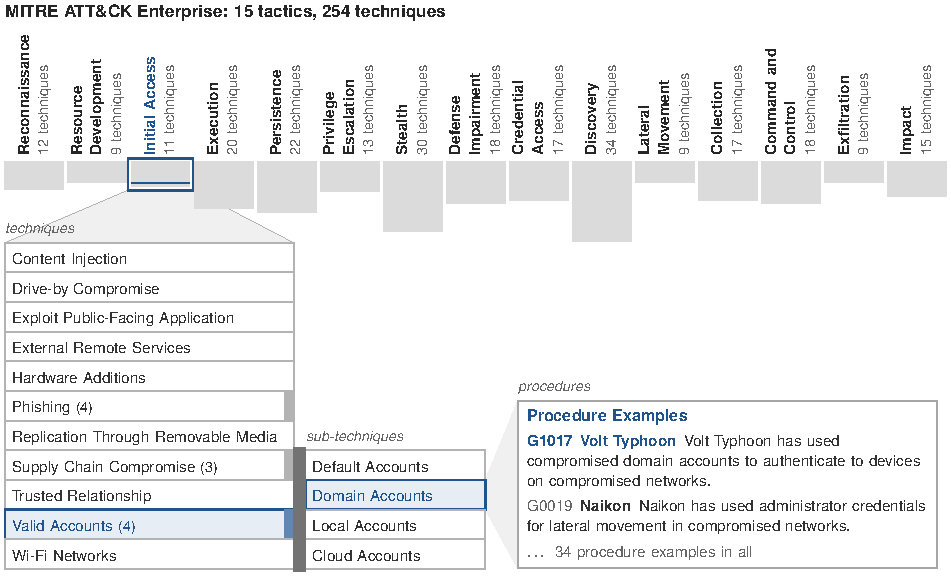
\includegraphics[width=\textwidth]{fig_3-1-2a_attack_matrix}
  % [CH3 REDRAFT ROUND 2, 2026-10-01, F1] figure rebuilt for its two takeaways (15 tactics holding the techniques; one technique opened to its sub-techniques and procedures): tactic names rotated and legible (about 8 pt printed; OVERTURNS the 2026-09-02 "stacked, never slanted" rule, Marc to rule), background cells plain, heading from the bundle. The trail above describes the old design. Caption ratify on read.
  % [CH3 REDRAFT ROUND 13, 2026-10-01, F1 caption] Shrunk to what the figure is and which path it opens; the reading instruction moved to the prose, "15 tactics" already in the figure's heading. Ratify on read.
  \caption[The ATT\&CK Enterprise matrix and its hierarchy]{The MITRE
  ATT\&CK Enterprise matrix (v19.1), with the Initial Access tactic opened
  down to a Volt Typhoon procedure \citep{mitre2026attackkb}.}
  \label{fig:attack-matrix}
\end{figure}

% 1 unit. Review Sec. III-D nearly verbatim (the review's exemplar
% section); closer from notes/ch3_lit_review/tactic_duration_precedent_survey.md.
% APPENDED 2026-09-02 (restructure ruling): the Attack Flow material
% from 3.1.2 now sits at the bottom of this subsection --- see the
% move comment there. Overdraft accordingly; reconcile at assembly.
\subsection{Attack profiling}
\label{subsec:profiling}

% [RESTRUCTURED 2026-09-03 --- Marc's shape ruling on the 3.1.3
% scrutiny: one subsection, no subsubsections; paragraph spine
% what+why -> gap -> other approaches -> Attack Flow -> what it does
% not carry. Applied here: arrangement, moves, and the approved cut
% list (log below); NO wording changed anywhere. Merge proposals ALL
% RULED 2026-09-03: M-A/M-B/M-C/M-E accepted (applied, tagged at
% their sentences), M-D inverted (prose keeps content, caption
% stripped --- see the figure comment). The missing so-what sentence
% is slotted for his dictation.
% Disposition of the 2026-09-02 append-move seams: (1) resolved by
% cut (2); (2) M-B pending; (3) M-A pending; (4) resolved by cut (3).
% The 2026-09-02 move provenance (appended-from-3.1.2 under his
% reversal of the 2026-08-31 no-split ruling) is recorded in the
% handoff, amendment item 13.]
% [CUT LOG 2026-09-03 --- approved cut list, do not re-flag:
% (1) "CTI, the raw material for this thesis, ranges from low-level
% indicators of compromise to structured descriptions of TTPs, and in
% its unstructured form (narrative reports, blog posts, vendor
% write-ups) requires manual normalisation before systematic use
% [ferraz2026]." --- wrong framing twice over, his rulings: the
% thesis's material is the Attack Flow corpus, not raw CTI, and the
% IoC-to-TTP ranging frame is ruled out. ferraz2026 keeps carriers in
% this subsection.
% (2) "The Attack Flow project [ctid2025attackflow] curates these
% incidents into structured records, and across them a group's
% toolchains and sequencing recur from one operation to the next: the
% consistency analysts rely on for attribution." --- dead referent
% ("these incidents"); recurrence is carried by the P1 motivation
% sentence; the attribution point does no work here.
% (3) "The analyst-curated Attack Flow corpus exemplifies the manual
% path: reliable structured representations from analyst review, at a
% pace and effort cost that limits coverage [ctid2025attackflow]."
% --- pre-empted the introduction; both its claims are carried
% verbatim by the corpus landing sentence in the Attack Flow
% paragraph.]
% [PASS 5 RULED 2026-09-03 (compress-to-ledger, split-stream WB+BB;
% merged ledger in chat). ACCEPTED and applied, deletion/merge only:
% X1 (corpus sentence moved above the curation reveal), X2 (opening
% paragraph merged into the gap paragraph), C1-C5, R1-R8, Q1, Q2,
% and --- Marc's follow-up ruling on read --- the full floor set
% F1-F5. Spine is now four paragraphs: what+why+gap -> approaches ->
% Attack Flow + artefact -> exit. Nothing left unruled from the
% merged ledger.
% PASS 5 CUT LOG (quotes abbreviated; full text in git history):
% (C1) "Because APT behaviour is both well-documented and recurrent,
%   it can be reconstructed into a reusable attack profile rather
%   than replayed as a single incident." --- resolves pass-4 TIGHTEN
%   M3 (durability carried at the chapter preamble, alshamrani2019);
%   the reconstruct-vs-replay contrast loses its prose carrier.
% (R1) the PM exemplar sentence (Rodriguez et al., process models
%   from event logs, Petri nets) --- PM now named-not-exemplified;
%   rodriguez2024 keeps carriers here and in 3.3; Petri precedent
%   carried by ch4.
% (F1) "Bridging this gap takes two forms, manual curation and
%   automated extraction, that trade coverage against fidelity."
%   --- the trade is carried by the strand verdict and "bought at a
%   coverage cost"; the approaches paragraph now opens cold on
%   "Automated extraction dominates".
% (F3) the figure-walk sentence ("This is the structure a linear
%   kill chain or flat intrusion-set membership cannot express ...
%   OR operator ... T1068 / T1552 -> T1078") --- the OR-join worked
%   example now lives in the figure alone (accepted with the ~5pt
%   portrait legibility trade known); the pointer folded into the
%   mechanics sentence per the fold licence.
% (F4) the terminal-condition block, Marc's dictated slot 3 of
%   2026-09-03 ("The terminal condition represents the objective of
%   Volt Typhoon here"; "This encapsulates something that may not
%   fit ... pre-positioning is not a technique"; the Cyber Kill
%   Chain contrast, hutchins2011) --- the restraint claim's carriers
%   are now the hand-curated README fidelity contract #3 and
%   cisaaa24038a.md Concepts 4-5, not thesis prose; hutchins2011
%   leaves this subsection (carriers ch2 l.536, ch4 l.2488);
%   cisaaa24038a keeps its prose carrier on the advisory sentence.
%   The slot-3 [3b]s ("the culmination", "other frameworks") and the
%   pre-positioning confirm-or-soften die with the block.
% (C2) "Attack Flow allows for more flexibility in encapsulating
%   preconditions and terminal objectives of APT attackers." ---
%   pure recap; no claim lost.
% (F5) ", as a human analyst would" --- analyst-parity carried by
%   the corpus sentence's "reconstructed by analysts".
% TIGHTEN log: Q1 (the which/how frame off the export sentence; the
% gap sentence's what/how carries the frame); Q2 (pivot merged into
% the definition sentence; "supplies exactly this missing structure"
% lost, carried by the mechanics and 57/16 sentences); F2 (STIX
% status clause; the claim moves to the oasis2021stix citation); R2
% (LLM-appeal foil; SoK verdict stands alone); R3; R5; R6; R7 + C5;
% C3 (the "; pre-positioning is not" tail --- then subsumed by F4);
% C4; R8 ("individual", "recent", "in 2022" --- the citation carries
% the source ---, "executable or" keeping "simulable").
% Mechanical repairs, flagged: "Automated" capitalised (R3), "The
% Attack Flow schema" capitalised (C4), "an" -> "a" before
% "simulable" (R8).
% RULING INTERACTIONS, both live for Marc's walk:
% (i) F1 + R6 together orphan "neither strand" in the exit paragraph
%   (the two-forms fork and "automated and manual alike" are both
%   cut) --- flagged [3b] at the sentence: revive one anchor or
%   accept the looser read.
% (ii) F3 inverts C5's premise (C5 deleted the curation sentence's
%   figure ref as the *second* ref; F3 then cut the first). Literal
%   application kept: the sole ref now sits as the fold parenthetical
%   on the mechanics sentence; [3b] at the curation sentence if the
%   ref should sit there instead.
% Marker dispositions: pass-4 TIGHTEN M3 resolved by C1; slot-4 [3b]
% "structure" resolved by deletion (R7); slot-3 [3b]s and the
% pre-positioning confirm-or-soften dead with F4. Still LIVE: [3b]
% "ATT&CK's" (M-B), [3b] "leaves them empty", the exit-paragraph
% half-order [3b], and interactions (i)-(ii).
% Overdraft ruling (Marc, 2026-09-03): ~2 units accepted for this
% subsection ("500-600 is gonna be alright"); the floor set landed it
% near ~450. The three-paragraph question (merge Attack Flow + exit
% paragraphs) re-answered in chat post-floor-cuts --- Marc's call.]

% [PASS 4 M1 RULED 2026-09-03 ("track the paper properly"): the trait
% triple restored to Rodr\'iguez's verbatim wording --- the draft's
% "objectives, motivations, and knowledge" was a paraphrastic
% substitution the extraction had already flagged (rodriguez2024.md
% Concept 2 / Concern 1: the paper's \S7 reads "objectives, knowledge,
% and modus operandi"). Do not re-flag.]
% [PASS 6 P1-signpost RULED 2026-09-03 (voice-pass, accepted): "ATT&CK's"
% prepended to the TTP list --- ties the section's opening definition
% back to 3.1.2's subject (the "what is it relating to" gap in Marc's
% read). Deletion/insertion of his own bridge noun.]
% [CH3 REDRAFT ROUND 2, 2026-10-01, 3.1.3 P1-P2] Narrative: what profiling recovers, the obstacle (named once, attributed), two routes (automated: scale, not yet reliable; manual: Attack Flow), the corpus and our drawn flow. STIX sentence cut (unused; its bib entry oasis2021stix was an unverified draft); "That manual path's exemplar" (Marc: unclear) replaced; ChronoCTI/AttacKG+ to one clause each; what/how italics removed. SESSION-DRAFTED on Marc's walk-through ("the narrative is a bit disjointed ... clarity and relevance"); ratify on read. Prior text in git.
% [CH3 REDRAFT ROUND 14, 2026-10-01, 3.1.3] Rebuilt on fixed terms, one per thing (Marc: "one of the poorest sections in terms of structure ... the terminology was not specific and not standardised"): attack profiling (automated / manual), attack profile, order, Attack Flow / flow / corpus, timing. "Extraction", "curation", "routes", "chain", "coverage against fidelity", "the difficulty", the procedural-semantics name, the export, the effect-edge mechanics and "Its main example" cut. Each sentence leads with its subject. Büchel's figures re-scoped to technique identification (what they measure). SESSION-DRAFTED on Marc's walk-through; ratify on read. Prior text in git.
\emph{Attack profiling} reads CTI to recover the order in which an
attacker used ATT\&CK techniques to reach its objective
\citep{rodriguez2024}. CTI records which techniques an attack used, but
rarely their order, and ATT\&CK does not record the order either
\citep{ferraz2026}. The product of attack profiling, an \emph{attack
profile}, can be executed as an attacker in a simulation;
Chapter~\ref{ch:attacker-model} builds its APT attacker model on attack
profiles.

Attack profiling is either automated or manual. Automated attack profiling
uses language models to recover the order from report text, as ChronoCTI
\citep{rahman2025} and AttacKG+ \citep{zhangY2025} do. It scales to many
reports, but even identifying which techniques a report describes is not
yet reliable: on the 50 most common techniques, the best systems reach
80\,\% precision at 66\,\% recall \citep{buchel2025}. In manual attack
profiling, analysts read a report and draw the order by hand. It is
reliable, but covers only the incidents analysts have drawn.

This dissertation uses manual attack profiling, with Attack Flow, a
language from MITRE's Center for Threat-Informed Defense (CTID) for
recording the order of an incident's techniques \citep{ctid2025attackflow}.
An \emph{attack flow} is one incident recorded in Attack Flow, from the condition
it starts in to the condition it ends in \citep{ctid2025attackflow}. CTID
publishes a corpus of attack flows that analysts drew from publicly reported
incidents \citep{ctid2025attackflow}. Figure~\ref{fig:attack-flow-volt-typhoon}
shows an attack flow drawn for this dissertation from the Volt Typhoon advisory
\citep{cisaaa24038a}.
% [DICTATED 2026-09-03 (slot 1: the so-what), repaired per pass 2+3a.
% Repair log: self-correction "execute sorry operationalise" resolved
% to the second form; "known defence mechanisms" (STT of "you know,
% defence mechanisms") -> "defence mechanisms" --- VERIFY; deletions
% "by"/"its"/"this" close the dangler ("by producing its ... this
% allows us"); pads dropped. The first formulation's reuse point is
% carried by "reusable". SCRUTINY: claim is in scope (matches the
% preamble's framing, no overclaim); "reusable" now appears here AND
% in the next sentence --- TIGHTEN candidate for pass 5.]
% [PASS 6 RULED 2026-09-03 (voice-pass, accepted): V1 "these profiles"
% -> "them" (doubled noun, pass-2 self-repair residue); V6 "moving
% target defence" -> "MTD" (defined at intro l.111 --- abbreviation
% after definition).]
% [C1 cut here (the APT well-documented/recurrent sentence, the
% ported 3.1.1-dissolve S4) --- see the pass-5 log above. X2: the
% paragraphs joined.]
% [M-B ACCEPTED 2026-09-03: subject repaired "These catalogues" ->
% "ATT\&CK's catalogues" (session-applied from the chat candidates).
% [3b] confirm the word on your walk. CITED (pass 4 M3, 2026-09-03):
% both prior candidates checked and neither carries the
% interchange-format claim per their extractions; a DRAFT bib entry
% for the OASIS STIX 2.1 standard itself (oasis2021stix) now carries
% it --- entry fields from session knowledge, marked VERIFY in the
% bib, confirm on read.]
% [F2 pass 5: the standard-interchange status clause cut; the claim
% moves to the oasis2021stix citation.]
% [M-A ACCEPTED 2026-09-03: opener "Yet this serialisation, the
% ATT\&CK-in-STIX export, records" -> "The ATT\&CK-in-STIX export
% records" --- deletion only; the sentence now reads as the gap's
% concrete instance. Do not re-flag the general/instance adjacency.
% Q1 pass 5: the which/how frame deleted; the enumeration stands.]

% [PASS 6 RULED 2026-09-03 (voice-pass, accepted): F1 REVIVED at the
% P2 head, superseding the pass-5 F1 cut. Marc's read named the
% automated->manual pivot as weak; the two-forms fork restores the
% antecedent that makes "that manual path's exemplar" land and gives
% "neither strand" (exit paragraph) its introduction --- fixing the
% pivot, interaction (i), and the missing frame in one move. His own
% words, restored verbatim.]
% [M-E ACCEPTED 2026-09-03, both trims applied --- do not re-flag:
% (a) PM tail "; the manual cost shifts from narrative curation to
% authoring and maintaining the technique-labelling rules" cut.
% TECHNICAL-CLAIM FLAG: the automation-isn't-free counterweight loses
% its carrier; the SoK verdict still carries the paragraph's
% conclusion. (b) NLP tail ", surfacing chains such as phishing
% followed by macro execution that individual reports describe in
% isolation" cut (second example; the 713/124 numbers stay).
% R1 pass 5: the PM sentence M-E(a) trimmed is now cut whole --- see
% the pass-5 log.]
% [PASS 6 RULED 2026-09-03 (voice-pass, accepted): V2 --- the naked
% "it" (plural subject "approaches ... combine", singular verb
% reaching into the appositive for ChronoCTI) given its head noun;
% the duplicated \citep{rahman2025} after "ChronoCTI" removed, the
% end-of-sentence cite covers both claims.]
% [M-C ACCEPTED 2026-09-03: tail ", at the coverage cost noted above"
% cut (referent died with cut (3); the claim's one carrier is the
% corpus landing sentence). Do not re-flag.]
% [PASS 4 minor SCOPE, ACCEPTED 2026-09-03: the verdict's subject
% narrowed --- the SoK's protocol covers NER / embedder / generative
% text extraction, not process mining (buechel2025.md), so "it" swept
% PM under a verdict never rendered on it. Session words "its
% text-extraction families" --- ratify on read.]

% [slot 2 --- session-proposed pivot RATIFIED in chat 2026-09-03
% ("just accept"); resolves the manual-path / "this missing
% structure" antecedent [3b]. Session words, ratify-on-read stands.
% Q2 pass 5: pivot merged into the definition sentence (pivot words
% verbatim as the head; "supplies exactly this missing structure,"
% deleted); R8: "in 2022" deleted.]
% [M-D RULED 2026-09-03, INVERTED from the session's proposal: the
% content lives in the PROSE; the caption is stripped lean (Marc:
% caption is AI-generated context, boil it to one sentence). This
% sentence stays in full. Do not re-flag the prose/caption overlap
% --- the caption side was the one cut.
% F3 pass 5: the figure pointer folded in as the parenthetical (the
% fold licence); the sentence itself untouched per M-D.]
% [F3 cut: the figure-walk sentence. F4 cut: the terminal-condition
% block (the dictated slot 3 of 2026-09-03, its VERIFY watchlist and
% walk-grounding record with it --- full provenance in git history
% and handoff item 13). C2 cut: the flexibility recap. All three per
% the pass-5 log above.]
% [X1 MOVE pass 5: the corpus sentence up from below the (cut)
% terminal-condition block, so corpus -> curation reads causal.]
% [DICTATED 2026-09-03 (slot 4: the corpus absence), repaired per
% pass 2+3a; full VERIFY watchlist in git history. Pass 5: R7 cut
% the "taking the CTI and condensing it into structure ..." clause
% (its [3b] "structure" resolved by deletion); C5 cut the figure
% ref; F5 cut ", as a human analyst would"; R5 cut "to do so".
% [3b] interaction (ii): the section's sole figure ref now sits on
% the mechanics sentence (F3's fold) --- move it to this sentence
% instead if the curated artefact should carry it, your call.]
% [PASS 4 minor SCOPE, ACCEPTED 2026-09-03: "no example Attack Flow"
% -> "no example Attack Flow in this corpus" --- the grounded claim is
% CTID-corpus-scoped (hand_curated README; cisaaa24038a.md Concept 5);
% the unscoped form asserted no flow exists anywhere. Antecedent is
% the corpus sentence above. Repair words session-supplied ---
% ratify on read.]
% [PASS 6 RULED 2026-09-03 (voice-pass, accepted): V5 "no example
% Attack Flow" -> "no example flow" --- Attack Flow reserved for the
% language, lowercase flow for an instance (terminology row ratified
% same day). The pass-4 "in this corpus" scope repair stands.]
% [PASS 4 M2 INSERT, ACCEPTED 2026-09-03 --- SESSION WORDS, ratify on
% read. The record's reserved argument (cisaaa24038a.md Concept 1:
% "the residual prose->structure gap the chapter argues";
% hand_curated README fidelity contract #2: 57 stated / 16 inferred
% of 73 edges): the section's own artefact quantifies the P2
% procedural-semantic gap, previously unclaimed here.]
% [PASS 6 RULED 2026-09-03 (voice-pass, accepted): M2 option A --- the
% appositive ": the procedural-semantic gap, measured on our own
% artefact" cut. Marc's read: the self-reference read "snarky and
% smarmy" (claimed to have arrived at the literature's gap by drawing
% a diagram); the numbers now stand as a plain fact. The P1 gap link
% is left for the reader to make (the gap is established in P1). Also
% resolves the S13/S15 skeleton echo the voice pass flagged. Reversible
% to option B (": an instance of the procedural-semantic gap") on
% read if the link should be explicit.]
% [CH3 SCRUTINY 2026-09-30, P10] the 57-of-73 sentence cut: unused later, and it counts the full flow while Figure 3.2 draws 13 edges. Prior text in git.
% [PASS 4 ACCEPTED-OPEN, placement yours (2026-09-03) --- two content
% candidates, this section or ch4; dictation slots once placed:
% (a) the prose never says the hand-curated flow stays OUT of the
% pipeline's corpus --- the README treats the exclusion as
% load-bearing (the GAP's author-independent provenance), and a
% reader here could infer the figure's flow feeds the build.
% (b) the other known non-carry: Attack Flow does not maintain
% motivation for APT groups (objective_pivot thread) --- the fact
% that forced L2's design; candidate for the strand-exit "what it
% does not carry" close, or ch4's story.]

% FIGURE --- the Volt Typhoon Attack Flow exemplar (replaces the Tesla
% placeholder; Marc's ruling 2026-08-31). MOVED with the Attack Flow
% material, 2026-09-02. Hand-authored from CISA AA24-038A,
% reduced to a teaching subset and restyled to the house palette; asset and
% pipeline in data/gap/hand_curated/ (README) and
% tools/restyle_attackflow_svg.py. Included portrait at \textwidth (Marc's
% ruling: no landscape); the figure is wide (2.46:1), so labels land ~5pt on
% the page, under the ~8pt guide --- a legibility trade accepted for portrait.
% CAPTION SESSION-DRAFTED --- yours for the voice pass.
% CAPTION STRIPPED to one sentence (Marc's M-D ruling, 2026-09-03:
% content in the prose, caption lean --- "reconstructed from the joint
% advisory, then the citation"). "reduced to its spine" retained as
% the honesty disclosure (the figure is a subset, not the full
% campaign) --- cut it on read if unwanted. The two claims that left
% the caption (restraint / corpus absence) RE-ENTERED VIA THE PROSE,
% Marc's dictated slots 3 and 4 (2026-09-03) --- both grounded (the
% old pass-4 KEEP: restraint = hand-curated flow's fidelity contract
% #3, corpus absence = the README's coverage-cost fact). None of the
% 13 exemplar nodes is touched by the v14->v19.1 deltas the README
% records.
% [CH3 REDRAFT ROUND 16, 2026-10-01, F2 placement] [htbp] -> [t]: it printed mid-page; top of page is the thesis's float convention (Marc's ruling on Figure 3.1, round 13).
\begin{figure}[t]
  \centering
  % [CH3 REDRAFT ROUND 14, 2026-10-01, F2] Redrawn natively (tools/attack_flow_figure.py, from the flow's STIX bundle): labels 8 pt (were ~5.4 pt), no technique ids, regular weight, conditions cut to their first clause; colour has one meaning (the two conditions), named in the drawing by role tags. The Builder export (tools/restyle_attackflow_svg.py) is retired from the tex. Caption: the takeaway only. Ratify on read.
  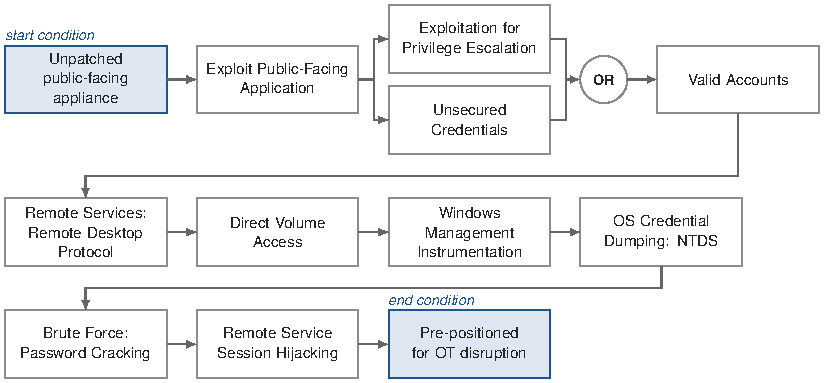
\includegraphics{fig_3-1-3a_attack_flow_volt_typhoon}
  % [CH3 REDRAFT ROUND 2, 2026-10-01, F2] T/F tabs removed from the figure; the caption says only how to read it. Ratify on read.
  % [CH3 REDRAFT ROUND 15, 2026-10-01, F2 caption] Provenance is the prose's ("drawn for this dissertation from the Volt Typhoon advisory"); start and end are the drawing's own tags. The caption names the figure.
  \caption[An attack flow of the Volt Typhoon campaign]{An attack flow of the Volt Typhoon
  campaign \citep{cisaaa24038a}.}
  \label{fig:attack-flow-volt-typhoon}
\end{figure}

% [moved 2026-09-03: the TI/IR sentence (the old verdict paragraph's
% closer) and the tempo material (was mid-section) now form the
% strand-exit paragraph --- the "what it still does not carry" answer
% to the capture strand's question. Original joint order kept
% (TI/IR -> tempo): "Yet" contrasts the corpus landing sentence above,
% the stitch chains off it. [3b]: this order ends the section on the
% ch4 dwell hook (month-granularity dates); swapping the halves would
% end it on the exit into 3.2's instruments instead --- your call.]
% [PASS 6 M1 RULED 2026-09-03 (voice-pass, accepted): the exit
% paragraph reworked --- claim-first opener assembled from Marc's
% chat seed ("attack profiling doesn't exist in MTD evaluation and
% we're missing tempo"), the two halves SWAPPED (tempo first, the
% TI/IR placement last, so the section ends on the 3.2 hook per his
% half-order ruling), and "automated and manual alike" REVIVED on the
% placement sentence (interaction (i) anchor for "neither strand";
% R6's "whole" stays cut). "And what neither strand supplies is
% tempo" fused into the tempo sentence at a colon (drops the
% sentence-initial And; voice-pass V8). Opener is assembled
% connective prose --- ratify-on-read.]
% [EXIT REWORK RULED 2026-09-04 (Marc, "looks good"): "Two gaps remain.
% Neither strand supplies tempo:" -> "The curated record supplies order
% and dependency, not tempo:" --- SESSION-PROPOSED WORDING, ratified in
% chat. His read of the old opener: a three-word declarative, more
% confident than the evidence, counting two things of different kinds
% (missing data in the record; where the apparatus lives) beside P1's
% procedural-semantic gap. The new opener is claim-first and pays the
% 3.1 interstitial's "which elements such a specification still
% lacks". "leaves them empty" -> "leaves them all but empty" in the
% same ruling, closing the pass-4 M3 [3b] on the measured margin (36
% of 38 flows empty; two carry epoch placeholders). "Neither strand"
% is gone, so P2's revived F1 fork no longer anchors it. Do not
% re-flag.]
% [stitch] the one after is from the precedent-survey note
% [PASS 4 M3 VERIFIED + carrier repair, 2026-09-03. (a) Schema half
% verified against the source markdown (2_1_attackflowdoc.md, the
% attack-action property table: execution_start / execution_end, both
% optional) --- ctid2025attackflow carries it; attackflow.md
% extraction extended with the record (Concept 5). (b) Corpus half
% MEASURED against data/gap/_corpus_stix/ (38 flows): 36 carry no
% timestamps; two (MITRE NERVE, DFIR BumbleBee Round 2) populate
% execution_start with 1970-01-01 epoch placeholders --- clock times
% only, no real-world dates. Substance of "leaves them empty" holds
% for all 38 (no machine-usable real-world tempo anywhere); the
% literal wording is falsified at the margin. [3b] keep "leaves them
% empty" or soften ("all but empty") --- RESOLVED 2026-09-04: "all but
% empty", per the exit rework ruling. (c) Cite carrier:
% month-granularity campaign dates are a catalogue-page fact, so the
% cite moves mitre2026attackv19 -> mitre2026attackkb per your
% 2026-09-02 carrier ruling (references.bib comment). Do not
% re-flag.]
% [C4 pass 5: "Public incident corpora encode order, not tempo: "
% cut (duplicated the stitch sentence) and ", the exact intended home
% for this data" cut. Pass 6: "And what neither strand supplies is
% tempo" fused into this sentence's head at a colon (V8).]
% [CONNECTIVE-PROSE PASS 2026-09-26, P7a 3.1 close] Split at the ruled
%  colon so the verdict stands as its own short sentence (the ruled 'not
%  tempo' kept). SESSION-GENERATED on Marc's 2026-09-26 go-ahead
%  (docs/workflows/connective_prose.md; audit
%  docs/implementation/connective_prose_audit.md); prior text in git.
%  RATIFIED 2026-09-26 (Marc: 'I accept all this').
% [CH3 REDRAFT ROUND 2, 2026-10-01, 3.1.3 P3] The strand exit: what a flow lacks (tempo), and where the apparatus sits. SESSION-DRAFTED on Marc's walk-through ("the narrative is a bit disjointed ... clarity and relevance"); ratify on read. Prior text in git.
% [CH3 REDRAFT ROUND 14, 2026-10-01, 3.1.3 exit] Claim first, then its evidence; "timing" for "tempo" (the plain word; tempo left 3.1.1 in round 11). The uncited "sits within the threat-intelligence and incident-response literature, outside MTD evaluation" narrowed to what the cited works themselves show (Marc: "is that the case ... it's an unsighted claim"); whether MTD evaluations use attack profiles is 3.3.2's to show. Ratify on read.
Attack profiling recovers the order of an attack's techniques, but not
their timing. Attack Flow can record when each technique started and
ended, but the attack flows in the corpus almost never do, and ATT\&CK dates each
campaign only to the month \citep{ctid2025attackflow, mitre2026attackkb}.
MTD must therefore decide when to move (Section~\ref{sec:mtd-concept})
without the attacker's timing. Deploying too often costs service
availability, and deploying too rarely gives the attacker time
\citep{cho2020}.
% [CH3 REDRAFT ROUND 19, 2026-10-01, 3.1.3 close] Marc: one long sentence lost the point; lead with what MTD has to grapple with. Split in two: the consequence (MTD decides when to move without the attacker's timing), then the stakes. Was (round 18): "Yet when to move, the third of MTD's design questions (Section 2.1), depends on the attacker's timing: deploying too often costs service availability, and deploying too rarely gives the attacker time." Ratify on read.
% [CH3 REDRAFT ROUND 18, 2026-10-01, 3.1.3 close] Marc: the right point to end on; say it with less. Two sentences to one: the fixed-interval prescription (a defender-design answer the chapter does not ask) cut; the cost-against-time balance kept as the reason timing matters; "Yet" carries the turn from the unrecovered timing. Ratify on read.
% [CH3 REDRAFT ROUND 17, 2026-10-01, 3.1.3 close] Marc: the timing line could be clearer and more relevant; his read that MTD's move to adaptive/hybrid triggers answers the cost of moving against the risk of not moving, under unknown attacker behaviour. Tied to ch2's when-to-move (Cho's three questions, Section 2.1). Grounding, Cho et al. 2020 Sec. II-B: "high frequency of MTD operations may incur high cost. Hence, an optimal MTD interval can be identified at run-time to balance both cost and security"; Sec. III: "when a defender has high uncertainty about an attacker's current activities and/or behaviors, it is better to trigger an MTD operation based on a certain, fixed time interval". Was (round 16): "Timing matters because MTD deploys its mechanisms once every deployment interval (Section 2.2.2), so when the attacker acts decides which deployments disrupt it." Ratify on read.
% [CH3 REDRAFT ROUND 15, 2026-10-01, 3.1.3] Read-through: "written in Attack Flow" -> "with Attack Flow" (profiling is not written); "An attack profile recovers" -> "Attack profiling recovers" (the process recovers, the product holds); the residual "None of the work surveyed in this section evaluates MTD." CUT (Marc: residual; the section closes on the limit). Ratify on read.
% [CONNECTIVE-PROSE PASS 2026-09-26, P7b 3.1 close] Second consecutive
%  X-not-Y made a plain locative. SESSION-GENERATED on Marc's 2026-09-26
%  go-ahead (docs/workflows/connective_prose.md; audit
%  docs/implementation/connective_prose_audit.md); prior text in git.
%  RATIFIED 2026-09-26 (Marc: 'I accept all this').

% ------------------------------------------------------ 3.2 evaluate --
% Feeds evaluate: the instruments are mature, and every one of them is
% scored over an attacker. 3 units (opener 1/4 + approaches 1/2 +
% metrics 1 + methods 1 + closer 1/4; amended 2026-09-05).
% PASS 6 RUN 2026-09-07 (voice-pass, white box, on the assembled 3.2;
% Marc: "I accept all the changes, a blanket"). Applied V1-V8 and the
% registry batch (defence mechanism canonical: opener "an MTD
% mechanism", 3.2.2 "MTD defence mechanisms", "MTD techniques"; cited
% authors as subject in the "et al.\ ... \citep" form: 3.2.1 S1).
% Session-chosen forms under the blanket: "a simulator" (V1), "This
% dominance" x2 with "This makes" kept (V3), "report" (V6), "The
% effectiveness metrics" without the instances clause (V8). Gate:
% 4 now passes; 7 partial resolved. DO NOT RE-FLAG: the three
% unit-closers on attacker assumptions (the strand's spine, not a
% duplicate --- handed to the integration check); the closer's "a
% single or small set of attacks" (Cho's phrase); the possessive
% "Jalowski et al.'s reading" (outside the ratified subject form).
% Section ~520 words vs 3 units. SECTION IS THROUGH PASS 6; the
% integration check is next. Outside this pass: the ch2 "MTD
% mechanism" sites (4) now fall under the ratified row --- a batch for
% ch2's next pass.
\section{MTD evaluation}
\label{sec:mtd-evaluation-survey}

% Strand opener (unnumbered, 1/4 unit). REWRITTEN 2026-09-07 (Marc's
% ruling on the cold read: the 2026-09-05 recast kept Cho's five-
% commitment anatomy plus a dispatch sentence and "in that order" ---
% the scaffolding cut from ch1 on 2026-08-21). Shape now mirrors the 3.1
% interstitial: S1 the strand's question, MARC'S DICTATION ("this
% section looks at how the field evaluates an MTD mechanism and the
% steps involved in such evaluation"; repaired: "dissection" -> "this
% section", "MTU" -> "MTD"; "looks at" -> "surveys" on his ruling the
% same day, matching 3.1's verb); S2 the sequence with the section
% references folded in as parentheticals (the ch2 MTDSim-preamble
% convention; the three nouns are the registry's ratified terms ---
% defence modelling approach / metrics / evaluation method --- so the
% thread and the headings agree). SESSION-ASSEMBLED S2 under the
% connective-prose green light, ratify-on-read. RULINGS, do not
% re-flag: the network model and attacker model are NOT named (ch2's
% preamble already frames MTDSim as network / defence / attacker;
% 3.3's interstitial opens on the attacker model); no citation (a
% signpost carries no cited claim --- the 3.1 rule; each subsection
% opens on Cho); no G1-style synthesis ("Each step carries assumptions
% of its own" was proposed as S3 and CUT by Marc as too strong);
% "evaluates ... evaluated ... evaluation" is a term repeat, ruled
% fine thesis-wide. Consequence noted: the dropped dispatch sentence
% was ch3's only statement of why the network model is not surveyed
% here --- the carrier is now ch2's preamble.
% SUPERSEDED (the 2026-09-05 recast, for reversibility): "An MTD
% evaluation commits to a network model, an attacker model, a set of
% defence mechanisms, a metric set, and an evaluation method
% \citep{cho2020}; the mechanisms are themselves designed under a
% defence modelling approach \citep[Sec.~VI]{cho2020}. Two of these are
% fixed by the simulator this thesis inherits, the network model
% (Section~\ref{subsec:network-model}) and the defence mechanisms
% (Section~\ref{subsec:defence-mechanisms}); the attacker model is
% Section~\ref{sec:mtd-attacker-models}'s. The three the field varies,
% the approach, the metrics, and the method, are surveyed here in that
% order." Before it, the ported sentence (Cho's own list, superseded
% 2026-09-05): "An MTD evaluation study selects a network setting
% (enterprise, cloud, software-defined, Internet of Things, or
% cyber-physical), adopts a threat model, deploys one or more MTD
% mechanisms, and assesses the result against a metric set using one of
% several validation methods \citep{cho2020}." Reorder ruled 2026-09-02
% (metrics before methods, Cho's Sec. VII -> VIII order) stands.
% [CONNECTIVE-PROSE PASS 2026-09-26, P5 3.2 preamble] Opens on the
%  three-step frame ('involves ... steps' is Marc's dictated phrase); S1
%  repeated the ch3 opener and was the third of four 'surveys' openers.
%  The 2026-09-07 rulings (no citation, no synthesis) hold.
%  SESSION-GENERATED on Marc's 2026-09-26 go-ahead
%  (docs/workflows/connective_prose.md; audit
%  docs/implementation/connective_prose_audit.md); prior text in git.
%  RATIFIED 2026-09-26 (Marc: 'I accept all this').
% [CH3 REDRAFT ROUND 2, 2026-10-01, 3.2 preamble] "Three choices" cut (Marc: it reads as a parallel of what/how/when to move); the section's question is where the attacker model enters. SESSION-DRAFTED on Marc's walk-through ("the narrative is a bit disjointed ... clarity and relevance"); ratify on read. Prior text in git.
% [CH3 REDRAFT ROUND 4, 2026-10-01, 3.2 preamble] "enters" -> how attacker models are used, one verb per step. Ratify on read.
% [CH3 REDRAFT ROUND 20, 2026-10-01, 3.2 preamble] Marc: a laundry list with no thread; then "too many clauses, de-fluff it". Link to the research question, the section's one claim (the result depends on the attacker model: what the 3.3 preamble reports back), then one short clause per subsection naming where the attacker model enters. Ratify on read. Prior text in git.
% [CH3 REDRAFT ROUND 21, 2026-10-01, 3.2 preamble] Marc: round 20 was vague and riddle-like; keep S1; name the parts by their terms; section numbers as subjects, not brackets; say why these three (Cho 2020 Secs VI-VIII: modelling and solution techniques, metrics, evaluation methods; his technique sections are ch2 2.1, his attack-model section is 3.3's source); no body-level instances (MTDShield) in a preamble. Ratify on read.
% [CH3 REDRAFT ROUND 22, 2026-10-01, 3.2 preamble] Marc: rounds 20-21 still unclear, "not on the right level of abstraction". Diagnosis: each round compressed a subsection's CONCLUSION about the attacker into a clause, which needs the subsection's concepts to parse. Now: say what each part IS; the selection criterion (the parts that use the attacker model, the ch3 opener's own phrase) answers "why three"; the attacker models themselves are 3.3's. "how and when MTD moves" ties back to 3.1.3's close. Ratify on read. Prior text in git.
% [CH3 REDRAFT ROUND 23, 2026-10-01, 3.2 preamble] Marc: S1-S2 and the metrics/methods clauses approved. "decide how and when MTD moves" is not how he would describe the approaches -> Cho Sec. VI's purpose ("modeling and solution techniques ... to develop MTD", each finding an optimal defence strategy / deployment), in ch2's ratified term *deployment strategy* (MTDShield is one, learned). Last sentence: "which attacker models?" -> the 3.3 preamble's own words. Ratify on read.
An MTD evaluation runs MTD against an attacker model and measures how MTD
performs. This section surveys the three parts of an MTD evaluation that
use the attacker model \citep{cho2020}.
% [CH3 REDRAFT ROUND 39, 2026-10-01, 3.2 preamble] Marc, whole-section read: each part's gloss repeated S1 and its subsection's opening definition (three copies in 1.5 pages). Glosses cut; each part is defined once, where its subsection opens. Overturns round 23's glossed list on merit. Ratify on read.
Section~\ref{subsec:defence-modelling-approaches} covers the MTD modelling
approaches, Section~\ref{subsec:mtd-metrics} the metrics and
Section~\ref{subsec:evaluation-methods} the evaluation methods.
Section~\ref{sec:mtd-attacker-models} then compares MTD attacker models with
the APT attacker.

% 1/2 unit. NEW HEADING 2026-09-05 (Marc's ruling, item 3): Cho
% Sec. VI, the theoretical approaches the DEFENCE is designed under
% (game theory, genetic algorithms, machine learning), carried here as
% an evaluate-strand commitment, not an attacker-modelling one. Why it
% earns a heading when this thesis uses none of them: three later
% arguments depend on it (the metrics unit's "dependent on the defence
% modelling approach" sentence; the criterion's two Cho Sec. V-D
% asymmetries, learning and rational-actor, granted to the defender;
% the gap's "rationality without capability"). GUARDRAIL (Marc's trap,
% 2026-09-05): this unit names where the FIELD's attacker comes from;
% the sentence "this thesis uses none of these" never appears here ---
% positioning on the ladder is ch4's opening. Shape mirrors the
% metrics unit: P1 the what (moved verbatim from the deleted 3.3.1
% "Attacker modelling traditions"), P2 the so-what (the attacker each
% approach imports --- the re-homed G4b, Marc's dictation). Heading +
% registry term "defence modelling approach" ruled 2026-09-05: the
% qualifier says whose model it is; bare "modelling" is the attacker's
% word in this thesis.
% [CH3 REDRAFT ROUND 20, 2026-10-01, 3.2.1 heading] Marc: "Defence" -> "MTD" (the 2026-09-30 bare-defence sweep); the qualifier the 2026-09-05 registry row asked for is kept. Label unchanged.
\subsection{MTD modelling approaches}
\label{subsec:defence-modelling-approaches}

% DRAFT STATE (2026-09-06): DICTATED by Marc, repaired (pass 2+3a) and
% 3b-walked the same session; every marker ruled, the three assembled
% sentences ratified on read. SUPERSEDES the ported P1 (review :55,
% moved here 2026-09-05): "Modelling techniques cluster into
% game-theoretic, evolutionary, and learning-based traditions, with
% game-theoretic formulations dominating by volume \citep{cho2020}. A
% representative game-theoretic formulation casts the defender as a
% leader committing to a configuration-switching strategy and the
% attacker as a follower that performs reconnaissance before launching,
% typically drawing on exploits from public enumerations such as the
% Common Vulnerabilities and Exposures (CVE) database, with attacker-type
% uncertainty encoded as a prior distribution \citep{cho2020}." The
% Stackelberg sentence is CUT on evidence: its specifics (attacker
% reconnaissance before launching, CVE exploits, a prior over attacker
% types) are not in Cho Sec. VI --- Cho describes leader/follower payoff
% only and never mentions CVE --- they are Sengupta et al.'s formulation
% ported under Cho's cite; nothing downstream referenced leader/follower.
% The [term] flag closes with the supersession (Marc's own noun,
% "approaches", now heads the sentence; triad in Cho's nouns per his
% "stick to Cho" ruling). G4b placeholder REMOVED --- P2 fills it.
% RULINGS 2026-09-06, do not re-flag: "There is no agency involved."
% cut as the duplicate; "tries to maximise reward functions in the
% short term" cut (Marc: the reward function is not the bad thing);
% the "no reward and cost functions in the real world" sentence not
% carried (same retraction); "often" hedges removed throughout (his
% ruling on the closing sentence, applied to the three in the ML run
% on his blanket accept --- reversible); "fantasy" -> "unrealistic";
% the beheaded P2 question stays beheaded. VERIFY (Marc): "PET models /
% PET simulators" heard twice, rendered "RL models / RL simulators"
% from context; the fitness-function sentence reads diversity in time
% and space INTO the fitness function where Cho VI-B ranks on attack
% resilience while seeking diversity --- his reading, ratified.
% Citation anchors: cho2020 at S1 and at the P1 run's end; cho2020 on
% the game-theory limitation (Sec. VI-A cons). The ML run has NO
% carrier in the bib (nearest: bland2020, tay2024; the CyberBattleSim /
% NASim keys of rl_security_environments.md are not in references.bib)
% --- open for pass 4. Pass-5 candidates noted: "not realistic ... based
% on unrealistic assumptions" doubling. ~210 words vs the 1/2 unit.
%
% PASS 4 RUN 2026-09-06, split-stream (WB main thread + BB subagent),
% merged ledger in chat; Marc RULED the same day. APPLIED: M1 (both
% streams) the machine-learning run SCOPED to the attacker a learning-
% based defence imports --- the opponent inside its training environment
% --- "reduces to an agent trying to fit to a training environment,
% instead of executing a campaign with a long-term objective, which is
% hard to encode" CUT (attacker-side RL framing, contradicted 3.3.3's
% Bland endorsement; "hard to encode" had no leg in the pack --- Marc:
% "the point is already made"); the earlier dictated head "is supplied
% by the training environment" REVIVED as the sentence; "and RL
% simulators" CUT (no bib carrier for the generalisation); cites tay2024
% (Sec. 7.1--7.2) + ho2024 (Sec. 5.1, 5.5) attached as the carriers.
% M2 (WB) the volume-dominance clause REVIVED on S1 from the ported
% sentence (3.2.2's "game-theoretic approaches often look at payoff and
% utility" is Cho :636's causal link to it). M3 (BB) "utility-maximising"
% -> "intelligent", Cho's own word (:508) --- Marc: "intelligent is the
% key word"; the WHICH-attackers scope stays open, see [3b]. MINORS all
% accepted: "attack model" -> "attacker model" (registry row 67); "(RL)"
% at first use; "and its usability" CUT (sense collision with Cho's
% security--usability tradeoff; restores the first dictation's close);
% the payoff-attribution [VERIFY] and the mechanisms/strategies noun left
% as [3b] --- both need his words. Consequence to note: the long-term-
% objective clause (ruled "a long-term objective" on the 3b walk) left
% with the cut sentence; revivable. Forward: the "ingrained into defender
% decision logic" close pre-states G1's first clause --- one home when
% G1 is dictated.
% PASS 5 RUN 2026-09-06 (white box), Marc APPROVED proposals 1--9, all
% deletion/merge: "amongst each other" cut; "rationality is assumed,
% and" cut (S2 carries it); "realistically" cut; "as a score of the
% fitness function" cut (claim flag: no-agency now carried by "no
% attacker as an agent" + the landscape metaphor; alternative kept in
% chat); S9+S10 merged at his dictated "which"; "very" cut; "of these
% RL models" cut; "are not realistic," cut (pass-4 doubling cleared,
% forced joint "and"); S12+S13 merged at "but" (sentence-initial But
% gone). ~230 words vs the 1/2 unit; three claim-level blocks (the S7
% "and" clause; the not-befitting sentence; the ingrained-into-decision-
% logic clause) presented separately; Marc ACCEPTED ALL THREE the same
% day. CUT with carriers: (A) "and a utility-maximising agent does not
% capture the complexity of an attack campaign or its long-term
% objectives" --- carried by 3.3.3's "rationality without capability"
% sentence and criterion properties (1)/(2); supersedes the marker-4
% assembly's second clause (its first clause, Cho's con, stays). (B) "The
% assumptions result in an attacker model that is not befitting of a
% real-world representation" --- tay2024/ho2024 cites MOVED onto the
% training-environment sentence (Tay Sec. 7.2 is a claim about the
% environment); "(RL)" abbreviation dropped with its only later use.
% (C) "In each approach, attacker model assumptions are ingrained into
% defender decision logic, but" --- premise restated by the conditional
% close; G1 (strand closer) now OWNS the clause. Unit ~175 words vs the
% 1/2 unit; residue is P1's five definitional sentences. Unit is through
% pass 5.
% PASS 6 RUN 2026-09-07 (voice-pass, white box, on this unit alone at
% Marc's scoping; ledger in chat; Marc BLANKET-ACCEPTED). Applied: S7's
% colon clause cut (restated its head); S3 "over ... over" -> "over ...
% against" (the pass-5 open item, closed); S6 "is a reduction of the
% agent's" -> "reduces to the attacker's" (nominalisation; the
% agent/attacker question resolved to the registry's canonical ---
% reversible); S1 recast active with \citet as subject, and "game-
% theoretic formulations" -> "game theory" (registry row 68, approach
% is the term); S9 "many" deleted (register b4, route (a); route (b), a
% dictated clause naming Tay 7.1--7.2 / Ho 5.1's actual assumptions,
% stays available); hyphenation "machine-learning approaches",
% "reinforcement-learning agents"; S10 "defence mechanisms" (number);
% S2 "an attacker and a defender". DO NOT RE-FLAG (ruled keep): the two
% three-beat walks (P1 "involve" x3, P2 "In ..." x3) --- enumerate-
% then-walk, not a tic; S5 "subsumed by the SDR operation alone"
% (clarity question posed, no change asked). Gate: 7 of 9 pass; P2
% claim-last by the 2026-09-06 beheading ruling (not a defect to fix);
% concreteness partial until G1's Tay sentence says what MTDShield
% trained against. ~176 words vs the 1/2 unit; overdraft sits until
% §3.2 assembles (2026-08-18 ruling). Unit is THROUGH PASS 6; the
% integration check runs on the assembled §3.2.
%
% [CH3 REDRAFT ROUND 24, 2026-10-01, 3.2.1 body] Marc: "a pretty poor section"; S1 led with Cho, not the subject; P2 walked the three approaches a second time and did not flow from P1; the MTDShield line was inserted bare; the closer ("If attacker models have no agency ...") condemned the field without evidence. Restructured: P1 says what an MTD modelling approach is FOR (the hole round 23 found; Cho Sec. VI "modeling and solution techniques ... to develop MTD", each finding an optimal strategy) in ch2's term *deployment strategy* (2.1.3: "decides which mechanism is deployed, and when"), then the three; P2 walks each approach ONCE, how it finds the strategy and the attacker it assumes, side by side; P3 the so-what with Cho's own evidence (Sec. VI-A, l.479 of the source: Carter vs Colbaugh and Glass, the difference traced to whether the attacker's goal required a persistent foothold), made explicit against 3.1.1, and closes on MTDShield. CUT: the "no agency ... logic limited" closer (no cite; the Cho evidence carries the point); "hindering the attacker's own learning" (off the deployment-strategy thread). Cites and ratified claims otherwise carried (Cho's con, Tay/Ho on the training environment, Tay on MTDShield). SESSION-DRAFTED, ratify on read. Prior text in git.
% [CH3 REDRAFT ROUND 25, 2026-10-01, 3.2.1 body] Marc on round 24: "each approach assumes an attacker" -- what does that mean?; "not necessarily rational or intelligent" -- why not?; ML's attacker "just happened to be there"; P3's opener vague and its two-studies sentence lost; MTDShield vestigial; and the dissertation's own strategies (random, alternative, single) come from no approach -- is that disjoint? Now: P1 says what the attacker is FOR (the strategy is found against a model of it); Cho's reason and consequence (VI-A cons: many attackers aim only to waste resources; the defender's best strategy may not work for irrational attackers); ML's attacker is what the training environment simulates; P3 opens on the claim, gives Carter's finding (via Cho VI-A, l.477) as the concrete case, then Cho's persistent-foothold tracing, then the APT consequence as its own sentence; P4 places Table 2.4's four strategies: only MTDShield comes from an approach, the other three follow a schedule. Touches the 2026-09-05 guardrail ("this thesis uses none of these" never appears here): NOT overturned -- the sentence places MTDSim's inherited strategies (ch2), not this dissertation's method. Ratify on read. Prior text in git.
An MTD modelling approach is a method for finding an optimal deployment
strategy. Cho et al.\ identify three: game theory, genetic algorithms and
machine learning, with game theory dominating by volume \citep{cho2020}.
Each represents the attacker differently.

Game theory models the attacker and the defender as rational players, each
choosing the strategy that maximises its payoff \citep{cho2020}. Attackers
are not necessarily rational: many aim only to exhaust a system's
resources, and a strategy found against a rational attacker may not work
against them \citep{cho2020}. Genetic algorithms search over defence
configurations for the one with the highest attack resilience and
diversity \citep{cho2020}. Their attacker is not an agent: it appears only
as the attack resilience the fitness function scores. Machine learning
learns a deployment strategy from the observed network state
\citep{cho2020}. Its attacker is the attacker model its training
environment simulates \citep{tay2024, ho2024}: MTDShield's is the baseline
attacker of Section~\ref{subsec:attacker-model} \citep{tay2024}.

% [CH3 REDRAFT ROUND 26, 2026-10-01, 3.2.1 P3] Marc: nuance the reader needs, not what the writer wants. One piece of evidence, the concrete one; Cho's persistent-foothold tracing cut here (it stays in 3.4's gap paragraph). Ratify on read.
% [CH3 REDRAFT ROUND 27, 2026-10-01, 3.2.1 P1 + P3] Marc: "against a model of the attacker" implies one portable attacker model, but GA's attacker is a fitness function and game theory's an agent -> "represents the attacker differently" (P2 then shows how). P3: Carter's platform-migration case was too specific and ran the argument backwards (a strategy good against persistent attacks, weak against fast ones; the dissertation's concern is the reverse); Cho's direction-neutral finding restored in plain words, as 3.4 states it. Ratify on read.
The attacker model therefore decides which deployment strategy is optimal.
% [CH3 REDRAFT ROUND 28, 2026-10-01, 3.2.1 P3] Marc: "persistent foothold" is never explained to the reader, so round 27 lost him; the platform-migration case was the clearer exemplar. Restored; its direction is made the dissertation's in the last sentence (a strategy found against fast attacks passes over the one that defends against persistent ones). "Persistent" is 3.1.1's defined word. Ratify on read.
% [CH3 REDRAFT ROUND 29, 2026-10-01, 3.2.1 P3] Marc: round 26's close was stronger; its negative framing ("may not be optimal against it") carries the conclusion even to a reader who missed the example. Restored. Ratify on read.
Migrating a service across diverse platforms, for example, defends against
persistent attacks but can weaken the defence against fast ones
\citep{cho2020}. An APT attacker is persistent
(Section~\ref{subsec:apt}), so a deployment strategy found against another
attacker may not be optimal against it.
% [CH3 REDRAFT ROUND 32, 2026-10-01, 3.2.1] Marc: P4 (MTDSim's four deployment strategies) is background, not literature. MTDShield kept as the surveyed instance of the machine-learning approach, folded into P2's ML sentence (Tay 2024 is literature); the scheduled strategies' clause dropped (ch2 2.2.2 already calls them proactive schedules). P3 is again the closer. Ratify on read.

% 1 unit. Families and origins only; the inherited suite's definitions
% (equation, direction) are ch4's under the 2026-08-21 metrics ruling.
%
% DRAFT STATE (2026-09-04): DICTATED by Marc, repaired (pass 2+3a) the
% same session. Shape ruled 2026-09-04 (handoff 2026-08-31_ch3_patchwork
% _draft.md items 16-17): two paragraphs, P1 the what (metrics as the
% precondition; the partition; the dynamic extension; the census), P2
% the so-what (the limitation block DICTATED below; its mechanism, the
% minority column + negative scope, and the scored-over pivot + handover
% are STILL TO DICTATE, see the [GAP] at the end of P2). Citations were
% attached from the cue card where the sentence tracks a source; pass 4
% confirms each. [3b] markers are Marc's. The ported review sentences
% this supersedes (review :57 verbatim) are kept below as SUPERSEDED for
% reversibility. Table 3.1 untouched (consolidation deferred).
%
% SUPERSEDED 2026-09-04 (ported text, for reversibility):
%   Cho et al.\ partition the MTD metric space along two axes
%   (Table~\ref{tab:mtd-metrics}): \emph{perspective} (attacker-side or
%   defender-side) and \emph{purpose} (effectiveness, capturing how well
%   the MTD reduces attack success, and efficiency, capturing the cost
%   the MTD imposes) \citep{cho2020}. Hong et al.\ \citep{hong2018}
%   extend this partition with network-state-dynamic measures (marked
%   $\dagger$ in Table~\ref{tab:mtd-metrics}) that quantify how the
%   security posture shifts as MTD operations execute across consecutive
%   network states.
\subsection{Metrics}
\label{subsec:mtd-metrics}

% 3b WALK RULED 2026-09-04 (Marc, spoken; applied): generic second
% person -> we/our (option 1); "threat model or attacker model" ->
% "attacker model" (his thesis-wide standardisation ask; conflicts with
% the RATIFIED 2026-08-20 registry row, so applied HERE only and raised
% as a PROPOSED refinement in terminology.md; the other 17 tex
% occurrences are listed there for his ruling); "your respective" cut;
% "attacker or defence" -> attacker-side / defender-side (matches the
% table); "mode of evaluation" -> "mode of modelling" (his suggestion,
% ratify-on-read; note the traditions unit is 3.3.1, not 3.2.2);
% "game-theoretic" -> "game-theoretic approaches" (his noun); the
% First/Second/Third walk DROPPED, the three reasons kept as
% complementary clauses in one sentence (deletion + commas only);
% "largest persistent issue" cited to all three surveys; the
% cross-technique sentence replaced by HIS chat reword (ratify-on-read).
% Citation faithfulness checked against the source markdown, each
% noted at its sentence.
%
% P1 --- the what. Question: what instrument does an MTD evaluation read
% its verdict from, and how does the field organise it?
% [CH3 REDRAFT ROUND 2, 2026-10-01, 3.2.2 P1 head] A metric defined; the purposes glossed in Cho VII's terms (effectiveness = attack and defence performance under MTD, VII-A l.574; efficiency = the cost MTD imposes on each side, VII-B l.640). SESSION-DRAFTED on Marc's walk-through ("the narrative is a bit disjointed ... clarity and relevance"); ratify on read. Prior text in git.
% [CH3 REDRAFT ROUND 31, 2026-10-01, 3.2.2 body] Marc: P1 disjoint (a heavy definition, the classification crammed into one sentence with "the cost MTD imposes on each", the game-theory exception, a census aside); P2 U-turns from metrics to "MTD mechanisms cannot be benchmarked"; P3 a lone sentence; Table 3.1 a side piece the prose never works through. Now: P1 defines a metric in the preamble's words, gives Cho's classification in plain terms (no "perspective/purpose/split/frame" meta-nouns: the table's own row and column names), then walks the table cell by cell with the metrics later chapters use (ASP, MTTC, NCR), and states the field's lack of a standard set as a fact about metrics (Cho VII l.568; Jalowski). P2 the attacker thread, made concrete: every effectiveness metric counts what the attacker does, so its value depends on how the attacker is implemented (Hong :73), and the consequence for an APT attacker, parallel to 3.2.1. CUT: the game-theory payoff exception (nuance not needed); "intractable cross-evaluation" folded into the no-standard sentence. SESSION-DRAFTED, ratify on read. Prior text and the ruling trail in git.
% [CH3 REDRAFT ROUND 32, 2026-10-01, 3.2.2] Marc: the efficiency sentence ran to five clauses; long sentences generally; P2's "every effectiveness metric" with a three-item list read as incomplete (and is false: time since last MTD is not counted from the attacker); "their values" vague. Now one clause per sentence where possible; metrics named, not redefined (definitions are 4.5's); P2 names its three metrics as its subject. Ratify on read.
An MTD metric measures how MTD performs. Cho et al.\ classify MTD metrics
as effectiveness or efficiency metrics, each either attacker-side or
defender-side \citep{cho2020}. Table~\ref{tab:mtd-metrics} gives examples of
each. Effectiveness metrics measure how well MTD stops the attacker.
Attacker-side effectiveness metrics measure the attacker's progress, such
as attack success probability (ASP) and mean time to compromise (MTTC)
\citep{cho2020}. ASP is the dominant effectiveness metric \citep{cho2020}.
Defender-side effectiveness metrics measure the network's security, such
as network compromise ratio (NCR) \citep{zhang2023}. Efficiency metrics
measure the cost of an attack or of MTD \citep{cho2020}. No standard set
of metrics exists \citep{cho2020}. Each evaluation chooses its own, so MTD
mechanisms cannot be compared across evaluations \citep{jalowski2026}.

ASP, MTTC and NCR are all computed from what the attacker does, so their
values depend on how the attacker is implemented \citep{hong2018}. MTD that
is effective against one attacker may therefore not be effective against an
APT attacker.
% PASS 6 V8 (2026-09-07, blanket accept): "Many of the metrics" -> "The
%   effectiveness metrics" (Table 3.1's honest scope; register b4). The
%   instances clause NOT taken (take-or-leave, left). Both [3b] closed.
% [3b] "Many of the metrics" --- the honest scope from Table 3.1 is
%   the effectiveness metrics (success events, attacker time, attack
%   paths, configuration space); "many" is the quantifier pass 6 cut
%   from 3.2.1 S9 (register b4). Keep "Many", or "The effectiveness
%   metrics"? Your call.
% [3b] your dictation also named the instances ("success events ...
%   vastness is dependent on the attacker's progress"). One clause is
%   available if the sentence should carry an example: ", success
%   events and time to compromise among them" --- session joint,
%   yours to take or leave.
% cite check: hong2018 :73 --- "their applicability is restricted to
%   the defined threat model, as the evaluation results are dictated by
%   the threat model used" --- said of the decision-theoretic IRS
%   approaches, not of MTD metrics; the cite carries the dependence
%   claim by analogy. Scope honestly if challenged.

% PASS 5 RUN 2026-09-04 (compress-to-ledger, split-stream WB + BB;
% Marc: "every single ruling I'm happy with" --- the FULL set). Applied,
% all deletion: P3 tail "and then from those values we can judge our
% defence mechanisms" (restated the effective-and-efficient
% apposition); P2 tail ", enumerating commonly used metric families in
% the literature" (the caption title carries it); P1 pads "Overall" /
% "heavily" / "particular"; P4 qualifier "that exists in the MTD
% literature". Caption: the selection-rule sentence, the
% citation-order sentence and the bold/shading sentence CUT (see the
% caption's own comment). DECLINED (do-not-re-flag): BB's cut of the
% whole opener colon clause (Marc's own words, today's ruled recast);
% BB's cut of the "no common benchmark" clause (the ruled carrier);
% BB's move of the ch4 pointer out of the caption (layout ruling 6);
% BB's tighten of the row-pairing decode (the only carrier of the
% pairing). Prose ~155 words vs ~250.
% THEN, same day, Marc APPROVED all four declined BB items ("I do
% approve those as well"), applied: the opener's colon clause CUT in
% full (SUPERSEDED: ": typically we have to instrument our model, run
% it and measure"); the "no common benchmark to measure effectiveness
% or efficiency" clause CUT --- HIS REVERSAL of the afternoon carrier
% ruling; "cannot be benchmarked" in the head now carries it, and the
% list's "and" moved to the third item (joint, ratify-on-read); the ch4
% pointer MOVED from the caption into the table sentence as a
% parenthetical --- HIS REVERSAL of layout ruling 6; the caption's
% row-pairing clause CUT (SUPERSEDED: "The two families on a row are
% one measure read from each side; " --- the pairing now has no
% decode; the empty-cell clause stays). Not applied: BB's whole-cut of
% the modelling sentence (L4), which BB itself declined by default; the
% bold/shading sentence stays cut (a ruling, not a BB proposal).
% CORRECTED same day (Marc: "no, there are no common benchmark I am
% keeping; in the caption, pointed to the layout, that's fine"): the
% "no common benchmark" clause REINSTATED (the afternoon carrier ruling
% stands, list "and" back on the fourth item); the ch4 pointer BACK IN
% THE CAPTION, the prose parenthetical removed (layout ruling 6
% stands). Standing from the BB set: the opener colon-clause cut and
% the caption's row-pairing cut. Prose ~130 words. Unit is through
% pass 5; pass 6 (voice-pass) runs on the assembled section.
% RULED 2026-09-04 (Marc): the remaining cue-card blocks are NOT
% dictated here. Mechanism (specificity vs portability) and the
% minority-column/deployment sentence DROPPED as symptoms of the
% benchmark gap ("moonlighting a critique"); the pivot + handover
% RELOCATED to the G1 strand closer below (the strand's argument, not
% the field's critique). The efficiency-column concession (no efficiency
% metrics reported; defender frozen) is a ch4 subsec:metrics disclosure,
% noted in the handoff. Unit ends here, ~205 words.

% TABLE 3.1 --- DRAFT STATE 2026-09-04, VERIFIED the same day by a
% split-stream pass on the table alone (white box in-session, black box
% subagent with the sources only; merged in the main thread; record in
% handoff 2026-08-31_ch3_patchwork_draft.md item 21, which also settles
% item 20's table findings). Marc's rulings on the merged moves:
% (1) ACCEPT --- repair the cites that fail the caption's own rule (DSP
% re-seated on Cho, jalowski2026 cut from unpredictability, the tempo
% row re-seated on Cho's periodicity, Kim named as his own variant);
% (2) "Basis" = the mechanism a family measures (the earlier "computed
% over" gloss was the looser reading; the header term may still
% change); (3) ACCEPT --- close the lineage-completeness gaps (Zhang's
% NCR, Tay's TSLM and downtime, Ho's host IP variability, Hong's
% ACE / ACD / NVDT / EVT). Then "mechanically fix and verify each
% outstanding issue": every non-KEEP finding is applied below or
% recorded here as a reasoned no-change.
%
% Layout (ruled 2026-09-04, variant D, unchanged): rotated purpose
% labels on the left, shaded with the row; Basis as the row key; the
% two perspectives as columns, a row = one measure read from each side
% (Cho's pairings ASP/DSP, MTTC/MTTF, the utilities, the costs; Cho's
% vastness-to-attack-surface link at his [114]; Zaffarano's mirrored
% Table 4); empty cell = no counterpart; zebra at black!5 continuous
% down the table; bold abbreviations; the rotated label sits in the
% LAST row of its block (negative multirow: -7 effectiveness,
% -3 efficiency). Needs xcolor[table] + multirow (preamble).
% Cell grammar (new): CITATIONS FOLLOW THE NAME THEY REPORT --- family
% name (ABBR) \citep{defining work, then the survey that lists it, then
% reporters}; variant name \citep{its reporters}. A key may sit by each
% name it reports (ho/tay by risk and by HCR); a group after a
% multi-name family means "reports at least one of these" (ho/tay
% report APE, not APV/APN). cho2020 is cited where Cho's list is the
% source of the family and no defining work is cited (ASP, DSP, the
% utilities, MTTF, unpredictability, vastness, CIA, periodicity, AC,
% defence cost, QoS); it is not cited where a defining work is (MTTC
% McQueen, attack surface Manadhata--Wing, RoA Cremonini--Martini,
% APV/APN/APE Hong).
% Selection (now stated in the caption): a family is in if a paper this
% review cites reports it, or Cho's census names it dominant, or Cho
% names it as the counterpart of one of those; the rest of Cho's
% Sec. VII list is omitted BY RULE --- learning by attackers /
% defenders [181], controllability [134], worm propagation speed
% [3][86][87], uniqueness / revocability / distinguishability [66][110],
% loss vs optimal deployment [141], strategy switching cost [141],
% power consumption [175]; Jalowski Sec. 2.3's policy-conflict analysis
% likewise. ho2024's "Attack Stage" is a state descriptor, not a family
% (no cell).
% Cell grounding (docs/sources/lit_review markdown :line unless noted):
%  R1 ASP: evans2011 = first ASP-for-MTD evaluation per hong:75 (bib
%     entry uncommented; VERIFY note kept there); cho:578; kim:408
%     ASP_REC / ASP_DEI; masud:432 Sec. 3.5.1; attack success zaf
%     Table 4; ASR ho:358, tay:286. DSP is Cho's coinage cho:594 ("We
%     call ... DSP in this work"); mission success zaf Table 4 (Cho's
%     exemplar [173]); attack actions blocked brown Fig. 4 :145
%     [VERIFY (1)]; detection
%     rate he:229-237 (Cho's DSP sense, his [38]).
%  R2 MTTC: mcqueen2006 = lineage root (extractions/mcqueen2006.md,
%     metrics_semantics.md; Cho's own MTTC refs are [4][26][27][32]
%     [186]; the word "mean" enters with Leversage & Byres 2008);
%     zhang:114; ho:372 (defined; used as an optimisation target
%     :503-517 [VERIFY (3)]); tay:286;
%     sharma:244 Eq. 2. ACD hong Sec. 5.1.5 / 5.3.5, expanded "attack
%     compromise duration" at zhang:254 (Hong never expands it).
%     Attack success time kim:406-414 AST_REC / AST_DEI --- named as
%     Kim's own variant rather than folded into MTTC (Kim has zero MTTC
%     hits), which closes the earlier VERIFY. MTTF cho:596 ("the same
%     as MTTC"); reliability alav:252-254, :265-268 ("under certain
%     attack circumstances", SHARPE) = Cho's "system reliability
%     metric" sense.
%  R3 utilities cho:580, :598; survey-only on both sides (Cho's
%     exemplars [22][134][141][181] are not in the bib; bland2020's RL
%     reward is the nearest chapter paper, not a game payoff, left out).
%  R4 APV/APN/APE hong Sec. 5.1.1-5.1.3 (across consecutive states);
%     APE ho:326, tay:238 / :286 --- Ho's APE is a per-host
%     new-vulnerability fraction on the shortest path at one time point
%     (hong2018.md open question; item 20 M1(f)), so the basis is now
%     "attack paths" (what both measure) without "across network
%     states" (Hong only); SAPV ho:384.
%  R5 attack surface mw:897 (methods, channels, data), cited to both
%     Manadhata--Wing works: the TSE metric paper (Cho's [112], obtained
%     2026-09-04) first, then the Springer formal-model chapter (Cho's
%     [114]) --- MOVED here from R4: it is not
%     computed over an attack graph or across states, the one cell
%     Marc's Basis ruling breaks; unpredictability cho:586 [66][110]
%     [145] (jalowski2026 CUT: it argues entropy, jal:125 / :151-163,
%     never names or reports the metric); vastness cho:618 "the size of
%     spaces that a given defense mechanism can cover", tied by Cho to
%     [114]'s attack surface measurements = the defender-side
%     counterpart, so the cell is no longer empty.
%  R6 attack confidentiality / integrity zaf Table 4 (Cho quotes both
%     at :604-606 but files them under the DEFENDER's CIA bullets)
%     [VERIFY (4)]; CIA + degree of
%     vulnerability cho:602-610; risk alav:252 / :272, ho:336, tay:286,
%     masud:436, sharma:336 / :396 (not a Cho Sec. VII name; Cho's
%     "degree of vulnerability" cites [4][5][6] = Alavizadeh's risk
%     papers); HCR ho:350, tay:234; NCR zhang:420. No source cites a
%     defining work for risk or HCR.
%  R7 periodicity cho:621 (Cho files it under EFFECTIVENESS, defender,
%     "other metrics" --- the row moved here from efficiency; "movement
%     tempo" was table coinage, dropped); MEF ho:366; TSLM ho:378,
%     tay:250; host IP variability ho:433; IP variation masud Sec.
%     3.6.1. In this thesis the interval is a swept PARAMETER (as kim
%     Table 4, zhang:418, brown:139); it is a metric family only under
%     adaptive schedulers (Ho, Tay) and in Cho's list.
%  R8 attack cost / payoff penalty cho:645-647; alav:253 / :326-331;
%     masud:442 (ho:348 defines AC as the time to exploit, inside RoA);
%     ACE hong Sec. 5.1.4 (:433 "attack cost of exploitation");
%     attempts required brown Fig. 5 :153, named as Brown's own
%     measure [VERIFY (2)]; RoA
%     cremonini2005 = defining work per alav:340 / :883-884 (bib entry
%     transcribed from Alavizadeh's reference list [VERIFY against the
%     original]), alav:340-353, ho:342, tay:286, masud:446 (also
%     "return on cost", :628). Defence cost cho:659; system performance
%     cho:658 (the family name was absent); mend Sec. 4.2 :744-893
%     (throughput, response time, total cost).
%  R9 QoS cho:653 (its own family in Cho and a service quantity, not a
%     resource --- split out of R8); mend:53; kim:394 FFJ "a QoS-based
%     performance metric".
%  R10 NVC / NVDT / EVC / EVT hong Sec. 5.2.1-5.2.4 in Hong's own words
%     ("variant assignment cost" :294-300, "edge variation cost" :320,
%     "edge variation time" :330; Hong never expands NVC / NVDT ---
%     Fig. 4c labels them "Node Defense Efforts"); node replacement
%     downtime tay:248.
% VERIFY --- Marc's four validation points (2026-09-04). Each is a
% classification call, not a checkable fact; "keep" = no change, "cut"
% = one deletion. The inline [VERIFY (n)] markers above point here.
%  (1) R1 defender-side "attack actions blocked" \citep{brown2023} as a
%      DSP variant --- Brown files it as attack effort (brown:200).
%  (2) R8 attacker-side "attempts required" \citep{brown2023} under
%      attack cost --- Brown declines cost / RoA / ASP (brown:141) and
%      reports attempts as attack effort (Fig. 5, :153, :200); item 20
%      M1(a) said cut when the cell was one citation group.
%  (3) R2 ho2024 as an MTTC reporter --- Ho defines MTTC (ho:372) and
%      optimises on it (:503-517); the outcomes Ho reports are ASR,
%      RoA, APE and risk (:483).
%  (4) R6 attacker-side "attack confidentiality and integrity"
%      \citep{zaffarano2015} --- Zaffarano's Table 4 is mirrored
%      (mission / attack); Cho quotes both at :604-606 but files them
%      under the defender's CIA bullets.
% Also for your read: the caption wording (DRAFT) and the header term
% "Basis" (gloss: "the quantity a family measures"). No citation cap
% (ruled 2026-09-04). \ref{subsec:metrics} points at the ch4 stub by
% design (the four reported families are MTTC, ASR, APE, RoA; the V2
% reworked-predictability measure may make it five).
\begin{table}[tbp]
  \centering
  % CAPTION PARED 2026-09-04 (pass 5, Marc's ruling: bare bones, decodes
  % only). CUT verbatim, revivable as a table footnote (conventions
  % §b4) if the concurrent table session wants the provenance under
  % the float: "A family is listed if a paper this review cites
  % reports it, if the census in Cho et al.\ names it as dominant, or
  % if Cho et al.\ name it as the counterpart of one of those; the
  % survey's remaining families are omitted." / "Citations follow the
  % name they report: the defining work where one is cited, then the
  % papers that report the family under that name or a variant." /
  % "Bold marks abbreviations; row shading is a reading aid only."
  % (the shading half was already ruled no-decode on 2026-09-04). Kept:
  % the axes decode, the Basis gloss, the row-pairing + empty-cell
  % decode, the ruled ch4 pointer.
  % THEN 2026-09-04, Marc approved the two remaining BB caption items:
  % the row-pairing clause "The two families on a row are one measure
  % read from each side; " CUT (no decode of the pairing remains ---
  % flagged risk accepted). The ch4 pointer was briefly moved to the
  % prose, then Marc corrected the same day: it STAYS in the caption
  % (layout ruling 6 stands).
  % CAPTION CUT TO THE TITLE 2026-09-04 (Marc's ruling, second caption
  % round): the purpose/perspective decode lives in the prose; Cho is
  % carried by the citation, not name-dropped; the Basis gloss cut ---
  % a header that needs a gloss is a bad header, so the header is
  % renamed (see below); the empty-cell decode and the ch4 pointer cut
  % as evident / not wanted. SUPERSEDED: "Metric families in MTD
  % evaluation, by purpose (row groups) and perspective (columns) after
  % Cho et al.\ \citep{cho2020}. \emph{Basis} is the quantity a family
  % measures. An empty cell means the family has no counterpart. The
  % four families this thesis reports are defined in
  % Section~\ref{sec:metrics}."
  % HEADER "Basis" -> "Measures" (session choice, ratify-on-read): reads
  % as the verb --- "attack success probability MEASURES success events"
  % --- so the column needs no gloss; alternatives "Computed over"
  % (the pre-ruling term), "Quantity".
  % FOOTPRINT 2026-09-04 (Marc: full page, floats away from the prose):
  % arraystretch 1.2 -> 1.0; Measures column 2.3 -> 1.9 cm; the two
  % perspective columns 5.5 -> 6.1 cm each (wider cells wrap less, so
  % fewer lines per row; textwidth is 16.06 cm). Type stays
  % \footnotesize (10 pt): the convention's floor is ~8 pt, which
  % \scriptsize sits exactly on --- available as a last resort, not
  % taken first.
  % [CH3 SCRUTINY 2026-09-30, T1] round-1 changes (X10-X12, option B, C3) are in git.
  % [CH3 REDRAFT ROUND 2, 2026-10-01, T1] Marc: "shrink it down ... what does a reader need ... what it counts, what does that mean". Now Cho's 2x2 itself: the "What it counts" grouping column is gone (it was this dissertation's, not Cho's); each cell keeps the metrics a later chapter uses (ASP, MTTC, NCR, attack actions blocked, the mitigation factor ch4's reductions take their form from, RoA) and enough of the rest to show the frame. Acronyms only where used again. Session-drafted, ratify on read.
  % [CH3 REDRAFT ROUND 31] caption: "frame of perspective and purpose" -> "classify", the prose's one verb; no meta-nouns. Ratify on read.
  \caption[MTD metrics]{MTD metrics as Cho et al.\ classify them
  \citep{cho2020}, with examples from the works surveyed.}
  \label{tab:mtd-metrics}
  \tablestyle
  \begin{tabular}{@{}lP{6.4cm}P{6.4cm}@{}}
    \toprule
    & Attacker-side & Defender-side \\
    \midrule
    \emph{Effectiveness}
      & Attack success probability (ASP) \citep{evans2011, cho2020, kim2026, masud2025}; mean time to compromise (MTTC) \citep{mcqueen2006, cho2020, zhang2023, ho2024}; attack path variation, number and exposure \citep{hong2018}; attack surface \citep{manadhatawing2011tse}; attack utility \citep{cho2020}
      & Defence success probability \citep{cho2020}; attack actions blocked \citep{brown2023}; network compromise ratio (NCR) \citep{zhang2023}; risk \citep{alavizadeh2022, ho2024}; mitigation factor \citep{alavizadeh2022}; time since last MTD \citep{ho2024, tay2024} \\
    \addlinespace
    \emph{Efficiency}
      & Attack cost \citep{cho2020, alavizadeh2022}; return on attack (RoA) \citep{cremonini2005, alavizadeh2022}
      & Defence cost and system performance overhead \citep{cho2020, mendonca2023}; quality of service \citep{cho2020, mendonca2023} \\
    \bottomrule
  \end{tabular}
\end{table}

% 1 unit. Review Sec. II-B para 1 + para 4. Renamed from "Validation
% methods" 2026-09-02 (Cho's own Sec. VIII title is "Evaluation
% Methods"; the anatomy sentence moved up to the strand opener). The
% MTDSim/HARM paragraph is ch2's; its first sentence (graphical
% security model + discrete-event simulation) is ch4's
% ladder-positioning sentence. Now 3.2.3 (2026-09-05); shape mirrors
% the metrics unit: P1 the what (the sentence below), P2 the so-what
% (G6 fused with the re-homed G4a --- the default attacker the
% graphical-security-model composition brings with it).
\subsection{Evaluation methods}
\label{subsec:evaluation-methods}

% CUE CARD (2026-09-07, scrutiny pass, Marc's ask): two paragraphs,
% P1 the what / P2 the so-what, mirroring 3.2.1 and 3.2.2. Brief by
% design (~120-150 w; the strand is well under its 3 units). EXISTS =
% carried by text already in the tex, skip on dictation; DICTATE =
% Marc's; DECIDE = his call before dictating. Keywords and cites only,
% no prose. Grounding: cho2020 Sec. VIII (source
% docs/sources/lit_review/1_1_cho2020toward.md, the VIII-A..D pros/cons
% paragraphs; extraction cho2020.md l.72 flexibility-vs-validity).
%
% P1 --- the what. Q: what evaluation methods does the field have?
%  S1 EXISTS, tidy: Cho's four categories --- analytical, simulation,
%     emulation, real testbed \citep{cho2020}. [term] "validation
%     methods" -> "evaluation methods" (heading, opener, registry all
%     moved 2026-09-02; this is the last prose occurrence).
%  S2 EXISTS, split off S1: analytical = probabilistic (SPN, ASP models)
%     / graphical security model (attack graphs, attack trees, HARM).
%  S3 DICTATE, optional, one sentence: what orders the four --- validity
%     gained against flexibility and scale lost (Cho Table VI; the
%     extraction's reading). Keywords per rung, Cho's own cons:
%     analytical = minimum cost, "simplicity and abstraction is
%     unavoidable"; simulation = parameterisable, sensitivity analysis;
%     emulation = higher validity, single-machine, no scale; testbed =
%     realistic, small/mid networks only. NOT "ladder"/"rung" in prose:
%     the fidelity descriptor owns "rung" (research gap), ch4's figure
%     owns "ladder" --- say "categories" / "methods" (registry row to
%     propose).
%
% P2 --- the so-what. Q: which method does the field use, and what does
% that choice cost? (mirrors 3.2.1 P2: the approach imports an attacker;
% 3.2.2 P2: the instrument cannot be benchmarked.)
%  S4 DICTATE: simulation dominates. Cho VIII-B first sentence, citeable
%     as is: "Most studies evaluating the performance of MTD approaches
%     have been validated based on simulation experiments"; VIII-C:
%     emulation "not as common as simulation studies" \citep{cho2020}.
%  S5 DICTATE: why --- Cho VIII-B pros: flexibility in modelling specific
%     attack behaviours, environments, MTD techniques; "most design
%     features can be easily parameterized without much restriction";
%     sensitivity analysis over key parameters; insight "before
%     performing the implementation in a real system". Keywords: high
%     abstraction, everything is a parameter, cheap to vary.
%  S6 DICTATE: the cost --- Cho VIII-B cons ONLY: "all possible
%     variables may not be captured" (uncontrollable uncertainty);
%     lessons "may not be realized in real testbed-based experiments or
%     systems". Keywords: abstraction, assumptions, transfer. SCOPE
%     guards: (a) "assumes an unrealistic attacker" is Cho V-D, not
%     VIII --- and 3.2.1 P2 already closes on it ("no agency ...
%     unrealistic assumptions ... logic of the defence mechanisms is
%     limited"), one home, skip here; (b) "we adopt a simulator and
%     wind back those assumptions" is positioning --- ch4's opening by
%     the 2026-09-05 guardrail (the review's :61 sentence is the
%     carrier available there; ch4's preamble does not yet say it).
%  S7 DECIDE, one sentence or none (G4a): the attacker the
%     graphical-security-model composition imports --- the graph's path
%     set, traversed; abstract, probabilistic, surface-directed.
%     Carriers: Cho VIII-A-2 (HARM: AG reachability over AT
%     vulnerabilities, [5][74][76]); hong2018 :73 "the evaluation
%     results are dictated by the threat model used"; masud2025 Alg. 2
%     as the instance (the cross-section's scripted row). NOT
%     hongkim2016: no source markdown in the repo, cited only for SDR
%     in ch2 --- do not attach unread. Earns its place because the
%     cross-section's Masud row and the gap's "parametric rung" both
%     lean on this default and nothing upstream names it; drop if the
%     unit is to stay purely about method.
%  S8 EXISTS, move up: the close --- single-mechanism evaluation is the
%     norm; multi-mechanism evaluation is a small but growing body.
%     The strand closer's Tay sentence carries it verbatim
%     ("reinforcement-learning orchestrators such as Tay's ... one
%     example among a small but growing body of multi-mechanism MTD,
%     and the broader paradigm inherits its training attacker from
%     whatever simulator it is built on") --- becomes this unit's last
%     sentence, or stays as the unnumbered closer with G1 cut: Marc's
%     call. Extra carriers if a lead-in clause is dictated: brown2023
%     ("singly and in combination", ch2 opener); alavizadeh2022
%     (combined S+D+R); chobenasher2018 (SPN integrated defence, MTD +
%     deception + IDS); masud2025 (coexistence rules); tay2024.
%  G1: CUT per Marc 2026-09-07 ("not even important") --- the
%     "ingrained into decision logic" clause is restated by 3.2.1 P2's
%     conditional close; 3.3's interstitial opens on the surveys'
%     diagnosis, so no synthesis is owed. OPEN: whether the cut also
%     covers G1a (the metrics unit's P2 tail) --- separate placeholder,
%     not mentioned.
%  The G6 (+G4a) placeholder was REMOVED 2026-09-07 with the dictation
%  (its text is in git history). S7 (G4a) RULED OUT 2026-09-07 (Marc:
%  "It's what we've inherited, which we describe in background
%  already") --- G4a is dead; the attack-graph attacker's home is ch2
%  §2.2.3 and the cross-section's Masud row. Do not re-raise.
%
% DRAFT STATE (2026-09-07): DICTATED by Marc against the card (S3, S4,
% S5, S6, S8), repaired (pass 2+3a) the same session; S1/S2 are the
% ported sentence split and tidied per the card. [3b] markers are
% his to walk; the verify watchlist and change log are in the chat
% return and summarised at each sentence. Citations attached where a
% sentence tracks a source; pass 4 confirms each. ~115 words vs the
% 1-unit ledger (card target 120--150).
% PASS 4 RUN 2026-09-07 (split-stream): the merged ledger sits under
% the strand closer below (M1 closer, M2 hinge insert, M3 routed to
% ch4). WALKED 2026-09-07: C1-C7 approved (C2 simplified to "multiple
% defence mechanisms together"; C4 re-routed to the introduction; C5
% landed as the ordering sentence). PASS 5 RUN 2026-09-07: P1 and P2
% applied, F1 (closer vs 3.3.1's V-D clause) left to pass 6 on the
% assembled 3.2. Unit ~160 words vs ~312. THROUGH PASS 5; pass 6
% (voice-pass) runs on the assembled section.
%
% P1 --- the what. Question: what evaluation methods does the field
% have, and what orders them?
% [CH3 REDRAFT ROUND 33, 2026-10-01, 3.2.3 body + the 3.2 closer] Marc: "a poorly written section ... short for the sake of being short"; S1 led with Cho, not the subject; the analytical split a decomposition the reader never uses; "flexibility and validity rise, scalability falls and cost climbs" a riddle; "variables a simulator does not capture limit what transfers" unreadable; the closer's five-paper mechanism clause off-thread. Now (Cho Sec. VIII, its pros and cons per method; V-D for the single-attack fact): P1 defines an MTD evaluation method in the preamble's words ("run MTD against the attacker"), names Cho's four with what each is, and states the trade-off at its two ends in plain words. P2: simulation dominant; MTDSim placed (Marc's ask, as fact from ch2); the limitation; the strength in Cho's terms (attack behaviours as parameters); the attacker fact last, as the bridge into 3.3. The separate strand closer (\medskip, round 2) and the comment trail between are folded in: its "varies the mechanism, not the attacker" contrast cut to the attacker half; the five mechanism cites dropped (each cited elsewhere). SESSION-DRAFTED, ratify on read. Prior text and the ruling trail in git.
% [CH3 REDRAFT ROUND 34, 2026-10-01, 3.2.3] Marc: S1 "the attacker" vague -> the preamble's own phrase (runs MTD against an attacker model); "Cho et al. name four" too choppy -> the four named in it. P2 went in four directions (dominance, MTDSim, limitation, strength, then a single-attack fact that read as a complaint against what was just praised). Now one line: why simulation dominates (Cho: models specific attack behaviours more flexibly than an analytical model), its cost in plain words (a result may not be reproduced on a real network; "every variable" cut: that is what a model is), and what that means here (MTDSim is a simulation, so an APT attacker model can be built in it). The single-attack fact is cut: it is 3.3's (Cho V-D, strategic plurality). Ratify on read.
An MTD evaluation method runs MTD against an attacker model. Cho et al.\
name four: analytical models, simulations, emulations and real testbeds
\citep{cho2020}. An analytical model computes the outcome
from a probabilistic or graph model of the network, the attacker and MTD.
A simulation runs a program that models them over simulated time. An
emulation runs real software on a virtual network, and a real testbed runs
on physical hardware. Analytical models are the cheapest to evaluate but
the most abstract \citep{cho2020}. Emulations and real testbeds are the
most realistic but hard to scale to large networks \citep{cho2020}.

Simulation is the dominant evaluation method, because it models specific
attack behaviours more flexibly than an analytical model \citep{cho2020}.
% [CH3 REDRAFT ROUND 35, 2026-10-01, 3.2.3 P2] Marc: "Its cost is that" a dangling pointer -> the results as subject; "so an APT attacker model can be built in it" implied no other method could -> the so-what is that this dissertation's evaluation takes both sides of simulation (S1's flexibility, S2's limitation). Ratify on read.
% [CH3 REDRAFT ROUND 36, 2026-10-01, 3.2.3 P2] Marc: S2 invites "why not?" -> Cho's reason in the sentence (VIII-B: not all variables captured, given real, uncontrollable uncertainty); S3 tried to restate S1-S2 -> what the reader needs is only where this dissertation sits; the paragraph above carries the rest. Ratify on read.
% [CH3 REDRAFT ROUND 38, 2026-10-01, 3.2.3 P2] Marc: filter and aggregate to what the reader needs. Three ideas, one sentence each: the strength (S1, kept), the limitation as the point it makes (results do not transfer directly to a real network; the reason folded into a relative clause), and what this dissertation does with the strength. "MTDSim is a simulation" dropped as known from ch2 ("MTDSim simulates ..."). Ratify on read.
Simulation results do not transfer directly to a real network, which no
simulation fully captures \citep{cho2020}. This dissertation uses MTDSim's
flexibility to run an APT attacker model through its existing attack
actions (Chapter~\ref{ch:attacker-model}).
% [CH3 REDRAFT ROUND 37, 2026-10-01, 3.2.3 close] Marc: the so-what is the strength the dissertation uses -- simulation's flexibility lets an APT attacker model be built outside the simulator and drive its existing attack actions (the ch4 opener: "shares the baseline attacker's attack actions, but its choice of the next tactic is set at runtime by the Petri net"); the limitation side is ch6's (sec:threats placeholder already lists "the six adopted attack actions" and "simulation only"). "That flexibility" points to S1. Ratify on read.
% C1 + C2 (pass 4 M1, APPROVED 2026-09-07, RATIFY ON READ). C1: "one
%   network model" DELETED (Marc: an oversimplification, "an irrelevant
%   point ... nuances need not be carried"); "one defence, one attacker"
%   -> Cho V-D's frame in his words ("one defence and a single small set
%   of attacks ... precisely what all my prior works did"); cite
%   localised to Sec.~V-D as in 3.3.1. C2: "hitting the frontier"
%   DELETED on the evidence (Cho IV-D catalogues hybrid MTD 2017-18; Cho
%   X names deployment of multiple techniques as the open item); Marc's
%   simplification ruling: the technique/mechanism altitude distinction
%   is his alone and confuses the reader --- say only "multiple defence
%   mechanisms together", and "where the recent work sits". Carriers:
%   chobenasher2018 DROPPED (IDS + deception + one MTD, not defence
%   mechanisms in ch2's sense); kim2026 ADDED (multi-phase MTD, the
%   cross-section's 2026 point); tay2024 kept (selector over the pool;
%   ho2024's pairwise combinations are the alternative if wanted).
%   SUPERSEDED: "MTD evaluation is mostly one network model, one
%   defence, one attacker \citep{cho2020}, but multi-mechanism
%   evaluation is hitting the frontier \citep{alavizadeh2022,
%   chobenasher2018, brown2023, masud2025, tay2024}."
% Dictated 2026-09-07 against the 3.2.3 card, repaired (pass 2+3a):
%   indirect "being" -> "is"; self-correction "hitting the field
%   hitting the frontier" resolved to the second form; "multi defence"
%   hyphenated then RULED "multi-mechanism" (whichever is more correct:
%   the registry noun); "one network" RULED "one network model".
%   VERIFY (mangle): "Wanna tackle" heard -> "one attacker" (Marc:
%   correct, "more of a colloquialism"). [3b] the triad's other two
%   nouns are unqualified beside "network model" (defence mechanism /
%   attacker model would parallel) --- his call at the voice pass.
%   cite: the one-mechanism norm is Cho Sec. V-D ("most MTD work
%   instead pairs one mechanism against one attack path") --- also in
%   prose at the criterion (3.3.1); one-home risk noted for pass 5
%   (Marc: "sure"). The multi-mechanism group is the card's carriers
%   (Alavizadeh combined S+D+R; Cho--Ben-Asher SPN integrated defence;
%   Brown "singly and in combination"; Masud coexistence rules; Tay's
%   selector) --- session-attached, trim on read (Marc: "sure").
%   RULED: "hitting the frontier" stays. Marc's gloss on the
%   sentence's intent (2026-09-07): multi-mechanism evaluation is the
%   paradigm shift, "and that's what we're adopting" --- the adoption
%   half is NOT in the sentence (positioning is ch4's opening by the
%   2026-09-05 guardrail; ch2's "singly and in combination" already
%   places MTDSim in that body).
%
% PASS 4 (2026-09-07, /scrutinise-draft, split-stream WB + BB, merged;
% Marc's ask "white and black box approaches"). Novel BB facts verified
% against their sources before entry; BB items that re-opened
% same-day rulings REJECTED and listed at the end. Content points only,
% wording his. Grounding: cho2020 source (lit_review/1_1_cho2020toward.md)
% Sec. IV-D :340-353, V-D :460, VIII-B, X :871; extractions/cho2020.md
% :103-112 (Table VI); implementation/architecture.md s(i) decision block
% and s(j) positioning; lit_review/alavizadeh2022.md abstract;
% extractions/{chobenasher2018,tay2024,masud2025,kim2026}.md;
% lit_review/brown2023.md :21-23.
%
% M1 --- THE CLOSER (both streams), four flags:
%  [WRONG, both] "one network model ... \citep{cho2020}": Cho V-D
%    bullet 2 (:460) says "a single or a small set of attacks" and few
%    scenarios with "multiple strategies ... by attackers or defenders".
%    Defence and attack(s): yes. Network model: NOT in Cho. The
%    single-network reading is the thesis's own from the Brown->Tay
%    lineage (architecture.md s(j): "single-mechanism, single-network
%    optimisation against procedurally-scripted attackers"). Either the
%    leg comes out from under the cite, or its carrier is the lineage
%    (ch2 / the 3.3.2 cross-section). Also: the section is V-D; 3.3.1
%    localises the same passage as [Sec.~V-D].
%  [VERIFY, BB, verified] "hitting the frontier": Cho 2020 has a Hybrid
%    section (IV-D, :340-353) cataloguing Alavizadeh S+R (2017), S+D,
%    S+D+R (2018), and Cho's own open item (X, :871) is "the optimal
%    deployment of multiple, hybrid MTD techniques ... has not been
%    investigated" --- existence is 2017-18, the open question is
%    evaluation/deployment. Two of the five carriers (chobenasher2018,
%    the Alavizadeh line) predate the survey the sentence contrasts them
%    with. "frontier" was RULED to stay as wording (3b); this is new
%    evidence on the CLAIM, so it is re-raised once, your call: Cho's
%    frame is "hybrid MTD is a recognised class whose evaluation is
%    under-developed", not "the field is arriving at it".
%  [VERIFY, both] the carriers: brown2023 YES ("combined effects of MTD
%    techniques", :21-23); masud2025 YES (S+D+R with coexistence rules);
%    alavizadeh2022 YES (abstract: "the combination of three MTD
%    techniques: Shuffle, Diversity, and Redundancy" --- source markdown
%    exists at lit_review/alavizadeh2022.md, NO extraction yet, so it is
%    cited on the abstract alone); chobenasher2018 is multi-DEFENCE (one
%    MTD + IDS + honeypot deception), not multi-MTD --- fits only if
%    "mechanism" is read as any defence, which ch2 s2.2.2 does not
%    (defence mechanism = SDR); tay2024 selects ONE technique per
%    decision (T-ACT-01; Ho's pairwise combinations, ho2024, fit the
%    claim better). kim2026 --- a multi-phase MTD framework in the 3.3.2
%    cross-section (extraction :30) --- is a 2026 carrier not cited.
%  [TIGHTEN, both] "one defence, one attacker" restates 3.3.1's second
%    dimension ("most MTD work instead pairs one mechanism against one
%    attack path"). Pass-5 one-home item, already logged; the closer's
%    own content is the multi-mechanism half.
%
% M2 --- [INSERT, BB, endorsed WB] the hinge into 3.3 that the Tay
%    sentence's loss opened (see TECHNICAL-CLAIM FLAG above): Cho
%    VIII-B says simulation's advantage over analytical models is
%    specifically "flexibility in modeling specific attack behaviors"
%    (periodic, DDoS, MAB-policy, sequential attacks). The dominant
%    method is dominant FOR attacker-behaviour flexibility; 3.3 then
%    finds the attacker model the field's weakest part. S5's "high
%    flexibility" is your word already --- the insert is what the
%    flexibility is for, one clause, and it carries the hinge at the
%    survey's level without the training-attacker clause. No
%    duplication with 3.3.1 (which carries the asymmetry, not the
%    method). Your call whether S5 or the closer takes it.
%
% M3 --- [INSERT, WB, routed OUT of this unit] "we adopt a simulator
%    and wind back its assumptions" (your opening ask, 2026-09-07) has
%    NO home: routed to ch4's opening by the 2026-09-05 guardrail, but
%    ch4's opening says "built beside MTDSim ... proof of concept" and
%    never says the method is inherited on purpose with its assumptions
%    wound back. Grounding: architecture.md s(i) ("the inherited
%    HARM-structural + DES-execution composition is treated as a
%    deliberate choice, not a default") and s(j); extractions/cho2020.md
%    disposition "adopted-as-baseline". Flag carried to ch4's opening.
%
% [KEEP, both] S1/S2 (Cho VIII opener + VIII-A split, verbatim in
%    sense); S3's testbed half (Table VI row 4 exact); S4 (VIII-B first
%    sentence + VIII-C "not as common"); no positioning, no ch2
%    re-description, no pre-claimed results.
% [VERIFY, both, no change] "remains": stands on Cho's 2011-2018 census
%    alone (ruled 2026-09-07); note the 3.3.2 cross-section names one
%    2026 physical-testbed work (kim2026) two pages on --- one work, not
%    a counter-census, but a reader sees it.
% [EXPAND, BB, minor] "Each evaluation method has its trade-offs"
%    promises four and gives two (simulation, testbed); Table VI rows 1
%    and 3 are one clause each if the promise is kept, or the promise
%    narrows. Your call; no table (ruled).
% [3b, WB, minor] S2 "graphical-security-model approaches" --- Cho's own
%    noun, but S4's "approach" -> "method" ruling reserved "approach";
%    keep as cited phrasing or align.
% REJECTED BB items (re-open same-day rulings; not for the walk):
%    [WRONG] simulation's abstraction cell (gloss RULED to stay);
%    [EXPAND] "low barrier to entry" as cause (gloss RULED); [REFRAME]
%    "defence mechanism logic" as Cho's consequence (RULED his
%    extension; the cite already sits after "simulator", so the cite
%    does not cover it); [REFRAME] closer intent vs G2's "the 3.2
%    closer" pointer (G2's pointer is stale --- re-point to 3.2.2's
%    closing sentence when G2 is dictated; logged).
% Pack note (both): no ch3 note carries evaluation-method material
%    (README scope note: the review was never mined); every claim here
%    stands on Cho and the cited works' own texts. Unit ~125 words vs 1
%    unit; the strand is under its 3 units by design.

% --------------------------------------------------------- 3.3 model --
% Feeds model: the field says so about itself; the rubric; the
% scoring; the gap. 4 units (interstitial 1/2 + 1 + 1 1/2 + 1).
% Subsection order swapped 2026-09-02: traditions before criterion.
% AMENDED 2026-09-05 (Marc's ruling, item 8): "Attacker modelling
% traditions" DELETED as a heading --- its Cho Sec. VI paragraph and
% G4b are 3.2.1's, G4a is 3.2.3's, Bland/Outkin are the gap's. Label
% subsec:modelling-traditions retired (its one referent, the gap's
% stitch, is replaced by the moved paragraph). Order is now instrument
% -> measurement -> verdict, the diagnosis stated ONCE, in the
% criterion, where it is the axes' source.
% [CH3 REDRAFT ROUND 41, 2026-10-02, 3.3 heading] RULED (Marc: "beautiful"): "Attacker models in MTD" -> "MTD attacker models", the chapter's one term for the thing. Label kept.
\section{MTD attacker models}
\label{sec:mtd-attacker-models}

% Interstitial (unnumbered, ~1/2 unit). Review Sec. IV-A cut to its two
% claims. CUT 2026-09-05 (item 7) to the move: on a cold read the
% diagnosis appeared three times (here, the criterion, the gap) and
% read as repetition; the sourced version lives in the criterion's Cho
% and Jalowski paragraphs. SUPERSEDED, reversible: "The persistence of
% this critique six years on is structural, not incidental: the
% attacker model MTD literature evaluates against does not match the
% attacker it claims to defend. Both surveys, however, stop at
% diagnosis: naming the attacker model as under-developed is not the
% same as measuring how far short any given evaluation falls, and
% neither survey resolves the critique onto specific papers, nor onto
% a scale against which an individual threat model can be placed."
% RECAST 2026-09-08 (Marc: the chronological survey rhetoric "is a bit
% much"; the section derives properties, applies them to recent works,
% defines the gap). Brought to the sibling pattern of the 3.1 and 3.2
% interstitials: one sentence of purpose, one of parts by pointer. CUT
% the timeline ("six years apart", "in 2020", "again in 2026"): Table
% 3.3's years carry the durability of the critique and 3.3.1 P1 carries
% the sourced diagnosis with locators. Connective prose, session-drafted
% under the connective-prose green light; RATIFY ON READ. SUPERSEDED:
% "Two MTD surveys, six years apart, identify attacker-model
% under-development as a primary limitation of the field. Cho et al.\
% \citep{cho2020} document it in 2020; Jalowski et al.\
% \citep{jalowski2026} document it again in 2026." and the stitch "This
% section draws the properties of a sophisticated attacker from the
% literature the surveys themselves draw on, and then measures."
% [CONNECTIVE-PROSE PASS 2026-09-26, P3 3.3 preamble] The cited survey
%  clause cut (it broke the 2026-09-05 'diagnosis stated once, in the
%  criterion' ruling and put a citation in a signpost); the 3.2-to-3.3
%  hinge carried by a pointer instead. SESSION-GENERATED on Marc's
%  2026-09-26 go-ahead (docs/workflows/connective_prose.md; audit
%  docs/implementation/connective_prose_audit.md); prior text in git.
%  RATIFIED 2026-09-26 (Marc: 'I accept all this').
% [CH3 REDRAFT ROUND 2, 2026-10-01, 3.3 preamble] The section's job (compare the field's attacker models with the APT attacker), linked back to 3.1 and 3.2. SESSION-DRAFTED on Marc's walk-through ("the narrative is a bit disjointed ... clarity and relevance"); ratify on read. Prior text in git.
% [CH3 REDRAFT ROUND 4, 2026-10-01, 3.3 preamble] "locates" -> "identifies the research gap"; "draws from the literature" -> "sets out ... that the literature says". Ratify on read.
% [CH3 REDRAFT ROUND 40, 2026-10-01, 3.3 preamble] Marc, preamble read as a CS student: it opened on a recap of 3.1 and 3.2 (defining itself by what came before), and its list sentence carried fluff ("MTDSim's baseline attacker among them", "missing from MTD attacker models"). Now leads with the section's reason in its own terms (an evaluation answers the research question only if its attacker model behaves like an APT attacker), then its job, then one plain sentence per subsection. The baseline attacker is named by 3.3.2's opener and the chapter intro; "lack" by 3.3.1's opener. Overturns round 2's recap opener on merit. Ratify on read.
% [CH3 REDRAFT ROUND 41, 2026-10-02, 3.3 preamble] Marc: round 40's lead read as a riddle ("only if ... behaves like one"). Now: the surveys' finding first (stated here once; 3.3.1's opener no longer repeats it), then the section's question, then one sentence for the two subsections. "checks", not "tests" (three works, not an experiment). Overturns round 40's lead, and the 2026-09-26 P3 ruling that kept the cited survey claim out of the preamble: the claim is the section's reason and is still stated once. Ratify on read.
Two surveys of MTD find that MTD attacker models lack properties of an APT
attacker \citep{cho2020, jalowski2026}. This section checks whether recent
MTD attacker models still lack them. Section~\ref{subsec:attacker-criterion}
% [CH3 REDRAFT ROUND 47, 2026-10-02, 3.3 preamble] "eight such properties" follows the new 3.3.1 heading. Ratify on read.
% [CH3 REDRAFT ROUND 57, 2026-10-02, 3.3 preamble] Marc: "needs to model an APT attacker" here too ("I would add that to the preamble 100 percent"). Ratify on read.
sets out eight properties an MTD attacker model needs to model an APT
attacker, and Section~\ref{subsec:recent-threat-models} scores three
recent MTD attacker models on them.
% [CONNECTIVE-PROSE PASS 2026-09-26, P3b 3.3 preamble] The properties' two
%  sources named (checked against 3.3.1's first sentence).
%  SESSION-GENERATED on Marc's 2026-09-26 go-ahead
%  (docs/workflows/connective_prose.md; audit
%  docs/implementation/connective_prose_audit.md); prior text in git.
%  RATIFIED 2026-09-26 (Marc: 'I accept all this').
% [CONNECTIVE-PROSE PASS 2026-09-26, P3c 3.3 preamble] The last part given
%  its dependency on the one before. SESSION-GENERATED on Marc's
%  2026-09-26 go-ahead (docs/workflows/connective_prose.md; audit
%  docs/implementation/connective_prose_audit.md); prior text in git.
%  RATIFIED 2026-09-26 (Marc: 'I accept all this').

% 1 unit. The eight properties DERIVED here as the literature's
% characterisation (port plan CONFIRM 2); ch4 cites them here (§4.1
% cut 2026-09-04; the scoring discipline --- badges, pre-commitment,
% rows A/B --- opens sec:fidelity-verdict, NEVER here). Property numbers
% are the criterion's (apt_model_criterion.md (c)) and are never
% renumbered.
% REBUILT 2026-09-07 on Marc's design rulings (trail: handoffs/
% 2026-09-07_ch3_s33_context.md §9): heading "Attacker model criterion"
% -> "Properties of a sophisticated attacker" (the old heading named
% the thesis's yardstick, which this section refuses to pose; label
% kept, ch4 l.~3348 and Table 3.2 \ref it); the FIDELITY DESCRIPTOR IS
% CUT with G3 ("qualitative, not backed up by anything, reads as
% tacky" --- the eight properties carry the verdict alone; six
% dependants re-pointed the same commit, each logged at its site);
% the two diagnosis paragraphs fused (the "six years later" repeat and
% the P1 alignment aside cut --- the interstitial owns the two-surveys
% frame, the merge sentence owns the 3.1.1 join); the nine-item
% enumeration sentence -> Table 3.2 (tab:attacker-properties); two
% unverified review glosses on Cho's characteristics cut (see P2).
% Shape: P1 diagnosis (what the surveys say is missing) -> P2
% description (what a sophisticated attacker is; the NIST merge) ->
% table -> P3 derivation (synthesis flag; the exclusion). Two DICTATE
% slots are Marc's. Locator convention (Marc's query 2026-09-07):
% IEEE numeric style renders the optional argument as [n, Sec. V-D] /
% [n, p. 8]; a page locator is required on a direct quotation, and a
% section locator is the convention for a section-specific claim from
% a long survey (Cho is 37 pages) --- whole-paper claims carry none.
% That is the rule the tex already follows (seven locator cites).
% [CH3 REDRAFT ROUND 41, 2026-10-02, 3.3.1 heading] RULED (Marc: "that's strong"): "Properties of an APT attacker" -> "Properties MTD attacker models lack"; the old heading read as a second definition of the APT attacker (3.1.1's job). Label kept.
% [CH3 REDRAFT ROUND 47, 2026-10-02, 3.3.1 heading] RULED (Marc): "Properties MTD attacker models lack" -> "Properties an MTD attacker model needs". Marc ruled the logic fix ("well thought through and well integrated"): the unit asserted its conclusion as its premise (the APT definition says what an APT attacker is, not what MTD attacker models lack; the surveys' evidence covers six of the eight). The criterion section now says what an MTD attacker model needs; the lack is the surveys' finding for six and 3.3.2's for all eight. Not "Properties of an APT attacker model": that is the name of this dissertation's model (ch4 on). Overturns round 41's heading ruling.
% [CH3 REDRAFT ROUND 67, 2026-10-02, 3.3.1 heading] "needs" read as a prerequisite for any evaluation; the research question's frame added, as in the 3.3 preamble and 3.3.2 P1 (Marc accepted).
\subsection{Properties an MTD attacker model needs to model an APT attacker}
\label{subsec:attacker-criterion}

% P1 --- diagnosis. Q: what do the surveys say the attacker model lacks?
% Ported (review :153, :155), verified against the source markdown
% 2026-09-07 (Cho V-D :454-464; jalowski2026.md §4.3). Two cuts, both
% Marc's rulings: "; most MTD work instead pairs one mechanism against
% one attack path" (the defence half of the same V-D passage is the
% §3.2 strand closer's --- one home) and "six years later" (the
% interstitial's). JOINT session-chosen, ratify on read: "Jalowski et
% al.\ reach the same diagnosis through ..." (was "... six years later,
% through ..."). [term] "threat-modelling assumptions" paraphrases
% Jalowski's §4.3 title ("Threat Modeling: Deconstructing Attacker
% Assumptions") --- cited-title language under registry row 67; swap
% to "attacker-model assumptions" if the paraphrase does not earn the
% carve-out.
% OPENER --- SESSION-DRAFTED 2026-09-07 on Marc's green light ("if the
% opening is just prescriptive I'm happy for you to draft something
% up"), RATIFY ON READ. Claim-first (clears gate check 1's soft fail)
% and the unit's one pointer at the table, placed before the source
% walk so the reader knows the table is coming. The close keeps only
% the ownership flag so the two do not repeat (Marc: "it's kind of
% repetitive").
% [CH3 SCRUTINY 2026-09-30, V1+V2] S1's source clause cut (the section preamble says it); the two paragraphs swapped so the reader meets what an APT attacker is (Cho V-A, properties 1, 4-6) before what the field lacks (Cho V-D, Jalowski), in Table 3.2's order; "also" moved; the synthesis sentence closes the unit. Prior text in git.
% [CH3 REDRAFT ROUND 2, 2026-10-01, 3.3.1 opener] the properties tied back to 3.1.1's definition (Marc: "I've already defined APT attacker and I don't really define these as properties of them"). SESSION-DRAFTED on Marc's walk-through ("the narrative is a bit disjointed ... clarity and relevance"); ratify on read. Prior text in git.
% [CH3 REDRAFT ROUND 41, 2026-10-02, 3.3.1 opener] the surveys' finding moved to the 3.3 preamble; the opener points at the table only. Ratify on read.
% [CH3 REDRAFT ROUND 42, 2026-10-02, 3.3.1 P1-P2] Marc, read as a CS student: lost at S1 (table-led; "the two surveys" unnamed; "the APT definition" unexplained), P1 re-defined the APT attacker (Cho's four characteristics restate 3.1.1, which already gives persistence, adaptivity, stealth and the objective-conditioned stages), "more or less" a hedge, the NIST/Alshamrani "overlap" sentence a machine-stitched join, P2 hard to follow, and Table 3.2 tacked on. REBUILT: P1 = where the eight come from (the 3.1.1 definition gives 1, 2, 4, 5; the two surveys, named, add 3, 6, 7, 8) + the table's job + the synthesis flag; P2 = the surveys' evidence that MTD attacker models lack them, each limitation followed by its property name in Table 3.2's words (the table woven in; the 2026-09-07 "(property n)" tags stay retired, the names do the mapping). CUT: Cho V-A's four-characteristic walk (3.1.1 and the table carry it; Cho stays cited on rows 1, 4-6), the NIST overlap sentence, "not a scripted intruder oblivious to the defence" (not-X-but-Y). Claims re-read against extractions/cho2020.md (V-D :454-464) and jalowski2026.md (4.3, p. 8). Ratify on read.
% [CH3 REDRAFT ROUND 43, 2026-10-02, 3.3.1 P1-P2] Marc: P1 on the right track but vague ("what definition?", "the choice of eight" vague, "defines each property by what an attacker model does" not specific); years for the surveys (recency is the point); keep prose and Table 3.2 consistent. P1 now leads with the claim (Marc's own order: "there are eight properties MTD attacker models lack; these are derived from ..."), spells out what 3.1.1's definition says for each of its four (term introduced in brackets after its gloss, the coinage convention), names the surveys with their years (descriptors, not the timeline rhetoric cut 2026-09-08), says why the merge is the dissertation's ("no single source lists all eight"), and gives the table its job (the behaviour 3.3.2 looks for). P2: once introduced, each property is used as a word in the sentence, point first ("they lack X: evidence"), not a bracket tag; Cho's third limitation now carries scheme awareness (V-D bullet 3, "leverage how MTD works", source l.462), so every Table 3.2 citation has its prose. Ratify on read.
% [CH3 REDRAFT ROUND 44, 2026-10-02, 3.3.1 P1] Marc: listing four properties "from the APT definition" under a claim about MTD attacker models misrepresents the backing (the definition is not MTD literature); point back to 3.1.1 instead of re-glossing it; drop the formalities (years, "survey of", "gap analysis"); subject first; "this dissertation synthesises these eight properties"; the table sentence read like a preamble. Now: S1 the synthesis and the table; S2 Cho's four characteristics (MTD literature, back in the prose, so Cho returns to rows 1 and 5); S3 the 3.1.1 pointer by name only, adding objective conditioning; S4 the three the surveys add. Definitions live in Table 3.2 only (one term, defined once): no bracket glosses in the prose. Overturns round 43's P1. Ratify on read.
% [CH3 REDRAFT ROUND 45, 2026-10-02, 3.3.1 P1] Marc: round 44 lost the narrative and the nuance; round 43 is the exemplar. Root cause: round 44 rewrote P1 wholesale instead of editing the sentences Marc flagged, answered his questions (pointer? brackets conventional? drop the years?) with cuts, promoted his synthesis sentence to the lead, re-added Cho V-A's walk that round 42 cut, and named "objective conditioning", "adaptivity" and "stealth" as terms 3.1.1 never introduces. Now round 43 restored as the base, with only Marc's round 44 points applied: the claim stands alone in S1, so the APT definition no longer reads as evidence for the lack (the misrepresentation); the definition is pointed to and its four terms coined in 3.1.1's own words (coinage convention: 3.1.1 describes, it does not name them); the years and "survey of"/"gap analysis" cut ("the two surveys" are the preamble's); the synthesis subject-first in Marc's words, with its reason, and the table folded into it (the separate table sentence read like a preamble). Cho cut from rows 1 and 5 again (round 43). Overturns round 44's P1. Ratify on read.
% [CH3 REDRAFT ROUND 47, 2026-10-02, 3.3.1 P1 S1] RULED (Marc): the claim becomes the criterion. Marc ruled the logic fix ("well thought through and well integrated"): the unit asserted its conclusion as its premise (the APT definition says what an APT attacker is, not what MTD attacker models lack; the surveys' evidence covers six of the eight). The criterion section now says what an MTD attacker model needs; the lack is the surveys' finding for six and 3.3.2's for all eight.
An MTD attacker model needs eight properties to model an APT attacker. The APT
definition of Section~\ref{subsec:apt} gives four: the APT attacker
pursues its objective over an extended period (persistence), acts after
the foothold according to its objective (objective conditioning), adapts
to the defender's resistance (adaptivity) and moves low and slow to avoid
detection (stealth) \citep{nist2011sp80039, alshamrani2019}. The two
surveys add the other four: strategic plurality, incentive-driven
rationality, learning and scheme awareness \citep{cho2020, jalowski2026}.
% [CH3 REDRAFT ROUND 46, 2026-10-02, 3.3.1 P1 close] RULED (Marc): "This dissertation synthesises the eight properties in Table 3.2"; the reason clause cut (the four-plus-four split already shows no single source lists them).
This dissertation synthesises the eight properties in
Table~\ref{tab:attacker-properties}.

Cho et al.\ name three limitations of MTD attacker models \citep{cho2020}.
First, they lack adaptivity and learning: the attacker follows fixed
attack patterns while the defender adapts and learns, although in
practice the attacker is often the smarter of the two. Second, they lack
strategic plurality: few evaluations let the attacker choose among
several attack strategies. Third, they lack incentive-driven rationality
and scheme awareness: the attacker is seldom modelled as a rational actor,
or as one that exploits how the MTD works. Jalowski et al.\ call the
attacker model ``the most glaring flaw in the MTD literature''
\citep[p.~8]{jalowski2026}. They find the same lack of learning and scheme
% [CH3 REDRAFT ROUND 47, 2026-10-02, 3.3.1 P2 close] Marc: "write that in, I'll read paragraph two and accept it or not". (a) Jalowski's sentence promised stealth after its colon but delivered stealth, learning and scheme awareness: split into one sentence per finding. (b) "the logic behind its movement" -> "the logic of the MTD scheme" (Table 3.2 row 8's words; "movement" is not a ch2 term). (c) The close names the two properties neither survey covers (checked: Cho V-D's three limitations, Jalowski 4.3), so 3.3.2 scoring all eight is the unit's answer to "who says they lack persistence?". The "most glaring flaw" quote stays. Ratify on read.
awareness: an APT attacker learns the MTD's deployment patterns over time
and looks for the logic of the MTD scheme \citep{jalowski2026}. They add
stealth: MTD is typically tested against active scanning, such as Nmap,
while an APT attacker uses passive reconnaissance to stay hidden
\citep{jalowski2026}.
% [CH3 REDRAFT ROUND 48, 2026-10-02, 3.3.1 P2 close] Marc accepted P2 up to its close, which read as tacked on: a negative lead ("Neither survey ...") and a signpost tail. Now the paragraph's point first (the surveys' evidence summed: six of the eight, the union of Cho's three limitations and Jalowski's stealth), then 3.3.2's job as the subject, with the two unassessed properties as the reason it scores all eight. "assesses", not "names": Cho V-A does name persistence, as a characteristic, not as lacking. Ratify on read.
% [CH3 REDRAFT ROUND 49, 2026-10-02, 3.3.1 P2 close] CUT both close sentences (Marc: "you can't read and write at the same time"). (1) "the two surveys find ... lack six of the eight" read as circular: P1 says four of the eight come from the surveys, so the surveys appeared to declare the properties and find them lacking in one breath; and the count adds nothing the three limitations and Jalowski's two findings have not already said. (2) The pointer to 3.3.2 repeats the 3.3 preamble ("Section 3.3.2 scores three recent MTD attacker models on them"); its reason (no survey assesses persistence or objective conditioning) left with round 47, since 3.3.1 no longer claims they lack those two: 3.3.2 scores all eight because they are the criterion. P2 now ends on its last finding. Ratify on read.
% PROPERTY TAGS RETIRED 2026-09-07 (Marc, second ruling the same day):
% the "(property n)" parentheticals read as an unordered scatter
% because the numbering is thematic (1--4 campaign half, 5--8 smart
% half) and the sources cut across it. The table's Source column
% carries the clause-to-row mapping instead; the opener points at the
% table once. Do not reinstate. Renumbering to first-appearance order
% was considered and declined (the axes are cited by number across the
% repo record; a thesis-to-repo mapping would be permanent).
% THE MERGE --- SESSION-ASSEMBLED 2026-09-07 from Marc's spoken gist
% ("persistence and adaptive behaviour are integral in the NIST
% definition; the objective conditions behaviour after the foothold;
% it's trying to mirror the NIST definition with Cho's enumeration,
% which was the inspiration"), RATIFY ON READ. Faithful: NIST (i)
% repeatedly over an extended period = persistence; (ii) adapts to
% defenders' efforts = adaptive; (iii) + Alshamrani Sec. II-C's
% objective-conditioned suffix = the objective. Filling the slot also
% fixes Marc's antecedent worry on "these sources" (Cho and Jalowski
% were the only authors named; Alshamrani was cited only in the
% table) --- the definition is now named in the prose before the
% pointer.
% P3 FOLDED into P2's close (2026-09-07): the old stitch head "Read
% together, these sources yield ..." and the synthesis flag are the
% unit's last sentence; "the merge of NIST's clauses onto Cho's
% characteristics" -> "the merge of the definition onto the
% enumeration" (the two nouns the sentence before it just used).
% EXCLUSION SLOT DROPPED (Marc's ruling 2026-09-07: "comes down to the
% discrimination of the literature review process; happy leaving it
% as is") --- do not re-flag. The unit is two paragraphs + the table.
% PASS 6 RUN 2026-09-07 (voice-pass, split-stream WB + BB, merged; Marc:
% "happy with all recommendations; where there was a failure of
% consensus side with the action"). APPLIED: Cho's "more or less" hedge
% carried; "the most harm" -> "serious harm" (Cho V-A :383, verified);
% the NIST/Alshamrani attribution split (NIST carries 1 and 4;
% Alshamrani Sec. II-C carries the conditioning claim) with the
% "is what conditions" garden-path repair; "higher level of capability"
% frame cut; "systematic" cut (not in Jalowski's record --- the word's
% only occurrence is a reference title), "gap-analysis" -> "gap
% analysis", "that names" -> ", and name"; S2 split at the appositive
% ("Cho et al.\ note that this asymmetry"); first tag carries the table
% ref; "as such" cut; "for a cost-effective outcome"; S6 merged into S7
% at a colon (S7 rides it for attribution); "mirrors" -> "overlaps
% with" (the honest scope); "adaptive behaviour" -> "adaptivity" (the
% row name); S11 commas dropped; the S5 clause "of MTD's design
% principles and threat-modelling assumptions" CUT (over budget + the
% registry row-67 breach) --- "of MTD" is the session joint, ratify on
% read; batch: "an APT" -> "an APT attacker", "Cho's" -> "Cho et al.'s";
% P2 opener varied with "also" (the identical-opener question, action
% taken). TABLE: NIST added to rows 1 and 4; rows 7 and 8 -> noun
% phrases; boundary clauses on 4 / 7 / 8 (reacts as they occur /
% retained across deployments / a model of the scheme) --- SESSION
% WORDS, ratify on read; "low-and-slow tempo" MOVED OUT of row 5
% (Alshamrani files it under persistent; row 1 carries the extended
% period) --- the criterion's §(c) row 5 still reads "low-and-slow tempo
% and evasion", to be brought to the table with the §(c) column (handoff
% §2); Cho V-D added to row 8 (bullet 3, "leverage how MTD works",
% :462); row 3's "rather than one attack path" cut (session-authored
% contrast). REJECTED at the merge (do not re-flag): BB's "mutation
% patterns" against the deployment row --- Jalowski's own phrase
% (:197), cited wording stays. HANDED to the integration check: gate 1
% claim-first is a soft fail by the ruled shape (source-walk openers,
% the claim lands last). Gate: 2, 3, 5, 7, 8, 9 pass; 4 and 6 clear with
% the batch; clarity clears. Unit is THROUGH PASS 6.
% TABLE RESTORED 2026-09-07: the round-2 fold deleted it by accident
% (the replaced span ran past it); recovered verbatim from 33c19763.
% TABLE --- the eight properties. RULED IN 2026-09-07 (Marc: "I'm happy
% with the table"), placed where the enumeration sentence stood. House
% style; caption = title only (Table 3.1's ruling). Rows in the
% criterion's §(c) order, NEVER renumbered (cited by number across the
% record, ch4 and ch7). CELLS ARE FACT-SCAFFOLD, session-typed from
% apt_model_criterion.md §(c) (sources) and §(d) (each axis's "what it
% is" line, compressed to a clause) --- RATIFY ON READ, wording Marc's
% to re-noun. Typed, not generated: eight rows and no data artefact
% (the tab:experiment-one deviation from the no-value-typed rule).
% Source column = the cell grammar of Table 3.1 (citations with the
% section locator; a key may sit on every row it grounds). Not in the
% table, by the §3 refusals: badges, "this model", the fixed-before-
% scoring provenance (ch7's), the word "criterion".
\begin{table}[tbp]
  \centering
  % [CH3 REDRAFT ROUND 7] caption reframed to the deficit (Marc).
  % [CH3 REDRAFT ROUND 42, 2026-10-02, Table 3.2] Marc: caption "are said to lack" not declarative; "What it names" vague; the Source column took most of the row; the cells not specific to attacker models. Caption now matches the 3.3.1 heading; the middle column says what an attacker model with the property does (each cell a verb phrase, meaning unchanged so Table 3.3's scores stand; "plural attack options" -> "several attack strategies", Cho V-D's word; "cost/benefit signal" -> "weighs the cost of an action against its benefit"); widths 3.2/5.9/5.3 -> 3.4/8.6/2.4 cm (same total). Ratify on read.
  % [CH3 REDRAFT ROUND 47, 2026-10-02, Table 3.2 caption] follows the heading: the table defines what is needed, not what is lacking.
  \caption[The eight properties an MTD attacker model needs to model an APT
  attacker]{The eight properties an MTD attacker model needs to model an APT
  attacker, and their sources.}
  \label{tab:attacker-properties}
  \tablestyle
  % [CH3 REDRAFT ROUND 43, 2026-10-02, Table 3.2] Marc: cells "so long and vague". Header "Definition"; cells cut to the behaviour scored (subject: the attacker model). Row 4 drops "changing conditions" (no Table 3.3 cell rests on it); row 8 "how and when the MTD scheme moves" is the wording 3.3.2's lineage cell (8) already uses; Cho cut from rows 1 and 5 (Marc: prose and table consistent; Cho V-A's characteristics no longer in the prose). Scores unchanged. Ratify on read.
  % [CH3 REDRAFT ROUND 44, 2026-10-02, Table 3.2] Marc: cells still vague ("reacts to the defender's resistance as it occurs" -- resistance to what? "including by"; objective conditioning hard to read). Cells now in terms ch2 has introduced (deployment, mechanism, disruption, attack action, foothold, campaign) and 3.1.1's objectives. Row 4 "chooses" keeps the lineage partial (its re-scan is forced, not chosen); row 7 learning = from observed deployments, row 8 scheme awareness = a model of the scheme's logic (the two kept apart). Cho back on rows 1 and 5 (P1 names his characteristics again). Scores unchanged. Ratify on read.
  \begin{tabular}{@{}rP{4.0cm}P{8.2cm}P{2.2cm}@{}}
    \toprule
    & Property & Definition & Source \\
    \midrule
    1 & Persistence & runs a multi-stage campaign over an extended period & \citep{alshamrani2019, nist2011sp80039} \\
    2 & Objective conditioning & acts after the foothold according to its objective, such as exfiltration or impediment & \citep{alshamrani2019} \\
    3 & Strategic plurality & chooses among several attack strategies & \citep{cho2020} \\
    4 & Adaptivity & chooses its next attack action in response to an MTD disruption & \citep{cho2020, nist2011sp80039} \\
    % [CH3 REDRAFT ROUND 46, 2026-10-02, Table 3.2 row 5] RULED (Marc): "instead of active scanning" cut; passive already says it (the CS reader knows the pair). "such as by" -> "for example by" (grammatical).
    5 & Stealth & avoids detection, for example by passive reconnaissance & \citep{alshamrani2019, jalowski2026} \\
    6 & Incentive-driven rationality & weighs each attack action's cost against its benefit & \citep{cho2020} \\
    7 & Learning & learns from the MTD deployments it observes, and keeps what it learns & \citep{cho2020, jalowski2026} \\
    8 & Scheme awareness & models the logic of the MTD scheme: which mechanism deploys, and when & \citep{cho2020, jalowski2026} \\
    \bottomrule
  \end{tabular}
\end{table}
% CUT 2026-09-07 (Marc's ruling), SUPERSEDED for the record --- the
% fidelity descriptor paragraph and G3: "Where those properties
% describe the attacker qualitatively, a fidelity descriptor captures
% what an attacker model \emph{actually does} at the level of attacker
% decision-making, ordered by depth from static parameters to learned
% behaviour: \emph{parametric} (success probabilities, fixed durations,
% or design-time parameters; no per-step decision during execution);
% \emph{scripted} (pre-coded sequences against specific CVEs or attack
% paths); \emph{procedural} (rule-based decision-making within an
% attack progression at runtime, beyond design-time configuration);
% and \emph{behavioural} (campaign-level intent, motivation
% conditioning, and learning capability). The descriptor is this
% thesis's own construction." + [GAP G3 earn the rungs]. The
% criterion's §(e) placement stays repo-side; ch7's fidelity verdict
% is the badge summary on the eight properties. Revivable from git.

% 1 1/2 units. Review Sec. IV-B compressed: the table carries the
% placements, the prose carries rhetoric-versus-execution. Brown + Tay
% -> one lineage column.
% RETITLED 2026-09-05 (item 9): "Threat models" -> "Attacker models",
% the thesis-wide standardisation; label kept (ch4 and G2 \ref it).
% REBUILT 2026-09-07 on Marc's rulings (trail: handoffs/
% 2026-09-07_ch3_s33_context.md §10, cue card §10.9). Shape: table
% first; P1 selection + warrant; one paragraph per table column
% (lineage / Masud / Kim), each claim-first on the executed attacker;
% the roll-call reading the table across all eight properties. CUT:
% the state-machine and scenario description (ch2 §2.2.3 carries it,
% Tables 2.2--2.3); Zhang's time-model sentence (the row-7 cell carries
% itself); Tay's IDS-sensitivity sentence AND the row-4 cell
% parenthetical (reverses port plan CONFIRM 3's sub-decision --- Marc's
% ruling; IDS as a thread was culled, handoff §3); He et al. from the
% prose as well as the table (Marc: MTD applied in another domain,
% adversarial ML on an NIDS, never directly portable --- port plan
% CONFIRM 3, he2025.md's semantic-scope contrast; he2025 stays a live
% bib entry, Table 3.1 cites it for detection rate); the descriptor
% residue ("parametric fidelity carries through", "scripted fidelity").
% MOVED: the rhetoric-versus-execution sentence, P1 -> the roll-call's
% opener (it is the pattern the three paragraphs walk, so it lands as
% a conclusion, not a promise). Every sentence below is ported
% (patchwork ledger l.1396--1495) or a trim of one; the three
% \emph{[DICTATE]} slots are Marc's. RATIFY ON READ.
% REDRAFTED 2026-09-08 on Marc's rulings (handoff §10.12 critique, §10.13
% scaffold): four paragraphs. P1 question / sample / pointer (G8 slot
% carries Marc's raw words, repaired for transcription only); Table 3.3
% moved to after P1; P2--P4 mirror A (what runs, with the authors' own
% scope statement inside it) -> B (the row read off dot by dot, then the
% empties), every clause line-anchored to the extractions' verification
% sections (docs/sources/extractions/*.md, "Eight-property
% verification"). Empathy residue stripped ("only", "candid",
% "genuinely", "claims more than this", "invoked taxonomically", the
% metrics-over-outcomes sentence --- 3.2's subject, and Brown's skill
% quote, which supported the cut descriptor and bears on none of the
% eight; SUPERSEDED: "Brown et al.\ are candid about the limitation,
% noting that ``the exploitation skills are not configured to
% distinguish the different skills of adversaries'' \citep[p.~7]
% {brown2023}."). The roll-call MOVED to a placeholder at the head of
% 3.3.3 (its across-columns sentence is the antecedent of "sharpens").
% Session-drafted from the record; RATIFIED ON READ 2026-09-08 after
% pass 6 (handoff §10.14).
% [CH3 SCRUTINY 2026-09-30, S2] heading was "Attacker models in recent MTD evaluations" (near-duplicate of the section heading).
% [CH3 REDRAFT ROUND 41, 2026-10-02, 3.3.2 heading] RULED (Marc: "beautiful"): "Recent MTD evaluations" -> "Recent MTD attacker models"; Table 3.3 scores the attacker model, not the evaluation. Overturns the 2026-09-30 S2 suggestion. Label kept.
\subsection{Recent MTD attacker models}
\label{subsec:recent-threat-models}

% P1 --- the question, the sample, the pointer. Q: what is measured and
% why these? G8 is Marc's; his raw words (2026-09-08) repaired for
% transcription only, one [3b] on the selection rule. The "gap" word and
% the answer both stay out (3.3.3's). The existing selection sentence
% is fused in; the per-work descriptors went to P2--P4's first sentences.
% RE-DICTATED 2026-09-08 (Marc), repaired per pass 2+3a, register
% sweep only; two [3b] RESOLVED by Marc's delegation 2026-09-08 ("carry
% these properties" for "achieve this fidelity"; "attacker modelling"
% per the registry). RULED OUT by Marc: the "favourable, hand-picked
% sample, existence not generalisation" clause ("obviously it's a
% favourable pick; don't say that"). Session note for the record, not
% prose: the clause was the answer to "why do three rows license a
% claim" (voice §c10); without it the warrant is "most likely to be
% grounded", which does the same job more quietly. Masud's ATT&CK
% mention is one sentence (l.299) and ATT&CK is absent from its
% reference list; Kim maps techniques throughout --- the keyword claim
% holds for both. SUPERSEDED first raw: "Having derived the properties
% a sophisticated attacker carries, the question is whether recent MTD
% evaluations carry them. Two works from 2025--2026 that frame their
% attacker on MITRE ATT\&CK were selected for that reason [3b], the
% works most likely to carry the properties, so the claim is existence
% over a favourable, hand-picked sample, not a generalisation; the
% simulator lineage this thesis extends is read the same way."
% DRAFT STATE (2026-09-08): DICTATED by Marc, repaired (pass 2+3a),
% [3b] resolved by delegation; unboxed for pass 4 (scrutiny) below.
% PASS 6 APPLIED 2026-09-08 (handoff §10.14, Marc's blanket accept):
% V1 recap opener cut (back-pointer folded into the closer); V2 "some
% form of" cut. P2: V4 MTDSim-first opener, V5 procedure sentence cut
% (ch2 duplicate), V6 clause cut, V7 riders cut, objective batch,
% disruption for block (registry RATIFIED). P3: V8/V9. P4: V7, V10.
% RATIFIED ON READ 2026-09-08 (Marc: "happy with this section now"):
% P1--P4 as applied, the count sentences kept, the W1--W5 conversions
% kept. Open: pass 5 to the ledger (584 / 375) and the 3.3.3 roll-call
% placeholder; G0 / M2 (the chapter's selection rule) is Marc's preamble
% rewrite.
% PASS 4 (scrutiny, 2026-09-08) --- three moves, Marc rules:
%  M1 [VERIFY] S2's selection rule. "A keyword search for MITRE ATT&CK"
%     appears nowhere in the record: the review's §IV-B states the
%     sample as spanning the lineage / IoT-cloud orchestration / NIDS
%     adversarial defence / a CKC-aware framework, no search; the port
%     plan (CONFIRM 3) and handoff §10.4 record He et al. as a THIRD
%     selected work cut 2026-09-07 as non-portable. If a search was run,
%     state index and date range as run; if the works were chosen by
%     reading, the sentence claims a method the record cannot back, and
%     "two works were selected" is post-cut (the submitted review shows
%     five). Masud's ATT&CK presence is one sentence (l.299; not in its
%     reference list) --- the search finds it, the warrant "grounded in
%     attacker modelling" leans on that one sentence.
%  M2 [SCOPE] collision with G0. The chapter preamble's G0 slot (l.~786)
%     promises ONE selection rule for the chapter, "first / most
%     established / latest" (port plan §3). S2 states a different rule
%     for this sample. Either P1's rule is the cross-section's own and
%     G0's is the strands', said so in G0, or one rule serves both ---
%     ruled when G0 is dictated; the two must not disagree on the page.
%  M3 [3b] register. "we then look at" is the only first-person plural
%     in ch3 prose; the chapter's agent is "this thesis" / "this
%     section" (interstitial: "This section draws ... and then
%     measures"; 3.3.1: "this thesis's own synthesis"). APPLIED
%     2026-09-08 by Marc's ruling: "this section asks"; first person
%     plural is licensed from ch4 on (the thesis's own model), ch1--3
%     stay impersonal. M2 is Marc's: he rewrites the chapter and
%     section preambles.
%  [KEEP] no result before the table (§10.2); the lineage's 2023--2024
%     against "2025--2026" is carried by S3; the reading rule lives in
%     the caption, not owed here.
%  [TIGHTEN, minor] S1 restates the interstitial's move one subsection
%     later ("having derived ... we then look"); "scores"/"scored" in
%     S3 and S4. [3b, minor] "some form of" is a hedge.
% [CH3 SCRUTINY 2026-09-30, R1/X9/C5] RULED (Marc): the works were chosen by reading, no search was run ("I read both their papers"); was "Two works from 2025--2026 were selected using a keyword search for MITRE ATT&CK, as the works most likely to be grounded in attacker modelling." His words: "the two most recent MTD evaluations that ground their attacker in ATT&CK"; "found in this review" scopes the superlative.
% [CH3 REDRAFT ROUND 41, 2026-10-02, 3.3.2 opener] the selection rule and the scorer stated, in the table's row order (yardstick (e)2, (e)5-6; checklist 7, 13). Session-drafted: "An attacker model grounded in ATT&CK is the most likely to have the properties" is the selection's reason (a most-likely-case sample: if these lack the properties, the gap is not an artefact of picking weak works); Marc owns it. "found in this review" kept (R1). Ratify on read.
% [CH3 REDRAFT ROUND 51, 2026-10-02, 3.3.2 P1] Marc: 3.3.2 read as an examiner (table-led, key in the prose, no signposts, a close that contradicted the marks) and Masud scored by a rule that zeroes any analytical model ("presenting a paper like that is so bad ... the properties are flexible, they can be applied to many attacker models"). All three rows re-scored blind, from the papers only, under one model-agnostic rule (evidence: extractions/brown2023.md, masud2025.md, kim2026.md, 2026-10-02); Marc: "the rescored table looks right". Overturns the 2026-09-07 'strict but generous' rule (a paper that runs no attacker earns nothing). Subject first; the selection rule made true (Masud names ATT&CK in one sentence and the kill chain; Kim's attacker follows the kill chain, ATT&CK maps its defence): "describe their attacker by the Cyber Kill Chain or ATT&CK"; the bar stated once, model-agnostic; the mark decode moved to the caption (results standard S4). Ratify on read.
% [CH3 REDRAFT ROUND 55, 2026-10-02, 3.3.2 P1] Marc: be specific (which eight properties, what "scored" means, who scores, what "recent" means: 2023 to 2026); "MTDSim lineage" -> MTDSim's baseline attacker (the ch2 term; Ho and Tay reuse Zhang's attacker unchanged, Ho l.242, Tay l.206, so the row cites Brown and Zhang only); the selection stated as this dissertation's expectation, not a fact; the superlative "the two most recent ... found in this review" cut (overturns the 2026-09-30 R1 wording: Marc, "we kind of just chose two recent papers"); "executed or computed" cut (3.2 carries it); the scoring rule stated as this dissertation's judgement, with all three marks and one worked example; the evidence pointer. Ratify on read.
% [CH3 REDRAFT ROUND 56, 2026-10-02, 3.3.2 P1] Marc: "needs" read as a prerequisite for any evaluation -> "needs to model an APT attacker" (the research question's frame, as Table 3.2's caption); the baseline attacker pointed to its ch2 section; the scoring rule was unclear ("what does model mean?") -> one sentence per mark, mark first, each tied to the property's definition in Table 3.2. The partial rule now names both routes the marks use: part of the definition (e.g. Kim's persistence, one short attempt) or a fixed rule or assumption in its place (e.g. the baseline's adaptivity). The worked example cut (the rule is now concrete; the baseline paragraph shows a tick beside a P). "gives the marks" -> "shows the marks ... cites the evidence". Edits round 55. Ratify on read.
This section scores three MTD attacker models, published from 2023 to
2026, on the eight properties an MTD attacker model needs to model an APT
attacker (Table~\ref{tab:attacker-properties}). The first is MTDSim's
baseline attacker, described in Section~\ref{subsec:attacker-model}
\citep{brown2023, zhang2023}. The other two are the attacker models of two
recent MTD evaluations that describe their attacker by the Cyber Kill
Chain or ATT\&CK, by Masud et al.\ \citep{masud2025} and Kim et al.\
\citep{kim2026}. This dissertation chose them because it expects an
attacker model described this way to be the most likely to have the
% [CH3 REDRAFT ROUND 59, 2026-10-02, 3.3.2 P1 example] Marc: "one response to each kind of disruption" is not hard-hitting. Now one concrete fixed rule a CS student sees at once against Table 3.2's "chooses": the baseline attacker always goes back to scanning hosts after a host-layer deployment (ch2 2.2.3; brown2023). Ratify on read.
% [CH3 REDRAFT ROUND 58, 2026-10-02, 3.3.2 P1 rule] Marc: round 57's P said the same thing twice ("has it in part: does part of") and lost round 56's second route; keep both routes, and make "stands in for it" plain. The colon glosses cut (the caption decodes the marks); the second route is now who does it, the authors, by a fixed rule (with the baseline's example) or an assumption (Kim's stealth); the cross is "neither applies". Overturns round 57's one-route rule.
% [CH3 REDRAFT ROUND 57, 2026-10-02, 3.3.2 P1 rule] Marc: standardise the term. "Score" is the act (S1, the Table 3.3 caption), "mark" the symbol; each mark is named by the caption's words, the words the per-model paragraphs use ("has", "has it in part", "has no"). The partial rule had two routes (part of the definition, or a stand-in); every P in Table 3.3 meets the first (checked row by row: each P does part of its definition and a fixed rule does the rest), so one route. "shows the marks" -> what the marks are of. Ratify on read.
properties. This dissertation scores each attacker model on each property
from its paper, with one of three marks. A \propmet\ means the attacker
model does all that the property's definition in
Table~\ref{tab:attacker-properties} says. A \propstandin\ means it does
part of what the definition says, or its authors set the behaviour by a
fixed rule, such as always re-scanning after a host-layer disruption, or
assume it.
A \propnone\ means neither applies. Table~\ref{tab:attacker-cross-section} shows each
attacker model's mark on each property, and the paragraph on each attacker
model below cites the evidence from its paper for each mark.
% [CH3 SCRUTINY 2026-09-30, T3] the mark decode moved here from the caption (no definitions in captions, supervisor 2026-09-22; yardstick §(e)3).

% TABLE 3.3 --- floats first (writing-guide order). REDESIGNED
% 2026-09-07 (Marc: the phrase-cell table "is not conveying what it
% needs to ... very sparse, lots of dashes, lots of words justifying
% what would otherwise be a tick"): back to the feature-matrix genre
% (conventions §e1 --- works as rows, properties as columns, no cross
% for absent) with THREE marks, not two, because the one thing the
% phrase cells were carrying was that a filled cell is not a property
% met: \CIRCLE\ met, \LEFTcircle\ something under the property
% operationalised without meeting it (the phrase now lives in the
% prose --- the lineage and Kim paragraphs and the roll-call's
% class (i) sentence, which must carry Zhang's cite for column 7),
% blank nothing. In this copy no cell reaches \CIRCLE; that absence is
% the table's message and the roll-call says it once. The ch7 copy
% adds the movement attacker's row, where the marks map onto the
% badges (demonstrated \CIRCLE, designed \LEFTcircle, not addressed
% blank) --- ch7's ruling, not made here. Heads: Table 3.2's names with
% their numbers, rotated (\rothead, the \rowgroup mechanism turned);
% years typed into the row labels (Marc: "a critical part of it is the
% year"; lineage 2023--2024, Masud 2025, Kim 2026), so the roll-call's
% close reads off the table. Width: 5.3 cm label + 8 x 0.85 cm + 8
% gutters (3.39 cm) = 15.5 cm (+0.4 for column 6) under the 16.06 cm textwidth; column 6's
% three-line head (1.27 cm) widens its column via \multicolumn{c}.
% ROUND 2 (Marc, same day): the decode re-anchored --- "met" read as
% "fully implemented", which nothing ever is (abstraction, assumption);
% the bar is now Table 3.2's one-clause definition: \CIRCLE\ has the
% property as Table 3.2 defines it, \LEFTcircle\ a feature under the
% heading that falls short of that definition. The lineage cite moved
% from the caption into the row label (genre §e1: citation in the row
% label, as Masud and Kim already had); the caption's lineage sentence
% cut (Table 2.1 defines the lineage). Heads as \multicolumn{1}{c} so
% a rotated block wider than its p-cell (column 6) widens the column
% instead of overfilling it; "6 Incentive-driven rationality" split to
% three lines so the header height is set by "conditioning".
% GLYPHS REVISED 2026-09-07 (Marc: with only the Harvey half on the
% page "it looks like MTDSim does everything"): stand-in = tilde
% (\propstandin), met = tick (\propmet, absent from this copy by
% construction, present in ch7's) --- Marc's own suggestion, in the
% genre; the greyed-ring interlude is logged in handoff
% 2026-09-07_ch3_s33_context.md §10.11 with the alternatives not taken.
% The comment below predates the glyph change: read its \CIRCLE as
% \propmet and its \LEFTcircle as \propstandin.
% HEADS, ROUND 2 (Marc: "for somebody who doesn't know the criteria
% ... initials or an abbreviation"): number over a short form ---
% Pers. / Obj. / Plur. / Adapt. / Stealth / Incent. / Learn. / Scheme
% --- in 1.15 cm columns (the widest short form sets it), which leaves
% 3.4 cm for the label, so every row label is set on two lines with
% the year on the second (consistent, and the years line up); marks in
% m{} columns so they centre on the two-line rows. Full text width.
% The number stays for the prose's by-number cross-references.
% HEADS, ROUND 1 (Marc, rendered and read: the rotated heads took
% ~2.3 cm for four rows of content, and the three-line "Incentive-driven
% rationality" head widened its column past the shaded p-cell, which
% broke the stripes): heads are the property NUMBERS, bound to Table
% 3.2 by the caption. Rotated one-word heads ("1 Persistence" ...) were
% rendered as the alternative and still cost ~2 cm; numbers cost one
% line and let the table sit at 14.3 cm, centred. \rothead stays in the
% preamble unused here. The stripe break was colortbl painting a
% p-column at its declared width while the \multicolumn head widened
% the column --- keep every head narrower than its column.
% MARKS --- EVERY CELL INDEPENDENTLY VERIFIED 2026-09-07 against the
% six source papers (one pass per paper, full text, not the
% extractions or the review); the line-anchored evidence is the
% "Eight-property verification" section of each extraction
% (docs/sources/extractions/{brown2023,zhang2023,ho2024,tay2024,
% masud2025,kim2026}.md) and the reconciliation is handoff
% 2026-09-07_ch3_s33_context.md §10.10. RULE (Marc, 2026-09-07,
% "strict but generous"): a half mark needs something the EXECUTED
% attacker DOES under the heading --- never a metric computed about it,
% a graph structure, or an evaluator's quantity --- so a paper that
% runs no attacker earns nothing; within that, interpretation is
% charitable. Lineage: 1 per-host loop repeated across hosts (Brown
% l.115; Zhang l.368); 2 two scenarios conditioning host preference
% and the give-up rule as a design-time rule (Brown l.109--111; Zhang's
% published model kept one, l.364 --- nuance ruled irrelevant, the row
% covers four works); 3 three vectors in a fixed fallback order (Brown
% l.115; Zhang l.376); 4 scripted responses to a block --- re-discover,
% re-scan, switch vector, restart from Phase 1, abandon after N
% interruptions, confusion penalty (Brown l.121/123/135/186; Zhang
% l.382/392); 6 RoA orders exploits within a host (Brown l.115); 7
% Zhang's halving, Eq. 2, per vulnerability, learns the network not the
% defender (l.392, printed p.30); 5 and 8 blank (active scanning; no
% model of the scheme; Tay's sensitivity knob verified defender-side,
% l.330; Ho adds nothing, l.573). Masud blank throughout: no agent
% runs, `all_simple_paths` (l.414); RoA is an outcome metric (RoCs =
% 1.01, l.586) consumed only by the defender's centrality ranking
% (Eq. 8, l.468). Kim: 1 three phase groups run in sequence by one
% script (l.276, l.282); 5 the outbound shell chosen "to evade the
% detection by a defense system such as a network intrusion detection
% system" (l.266, p.7), executed but untested --- no detector in the
% testbed (l.450); 2, 4, 8 blank (one objective, fixed behaviour; T_k
% is the evaluators' quantity; the scan range is the experimenters'
% knob). Locators verified: Brown p.7, Masud p.7, Kim p.7 §5.2. Port
% plan CONFIRM 3's "phrase cells over ticks" is REVERSED by this
% ruling; the phrase-cell copy is in git at ba253287 (SUPERSEDED). No
% column for this thesis's model here (handoff §3).
% LAYOUT RULED 2026-09-07 (Marc, "C is probably the best", after four
% variants rendered at print size): condensed one-line rows --- 3 pt
% \tabcolsep inside the table, 1.1 cm mark columns, column 8 at 1.15 cm for "Scheme" (the narrowest the
% short-form heads fit without breaking the stripes), the label column
% at its natural width with the year inline (supersedes the two-line
% label ruling of earlier the same evening); just under the text width, not
% full width. Applied identically to Table 7.1 (tab:fidelity-verdict)
% in the same commit --- the two must not drift.
% [CH3 REDRAFT ROUND 50, 2026-10-02, Table 3.3 layout] Marc: the table ran 1.1 cm past the text width (the lineage label's citations set the l column), and the two tables split the 3.3.2 opener across three places. Label column fixed at 4.3 cm, ragged right (only the lineage label wraps, after its years), so the table is 14.8 cm; [t] so Tables 3.2 and 3.3 stack at a page top and the text runs on below them. Applied identically to tab:fidelity-verdict (the two must not drift).
\begin{table}[t]
  \centering
  % [CH3 REDRAFT ROUND 42, 2026-10-02, Table 3.3 caption] "Attacker models in recent MTD evaluations" -> "Recent MTD attacker models" (round 41's one term, the 3.3.2 heading). Ratify on read.
  % [CH3 REDRAFT ROUND 51, 2026-10-02, Table 3.3] re-scored (P1's comment); the marks decoded here (results standard S4; Bonneau's legend); "MTDSim" with its four citations, the years in their own column, eight equal mark columns (Marc: "MTDSim spanned out too far").
  % [CH3 REDRAFT ROUND 52, 2026-10-02, Table 3.3 caption] Marc: "has the property in our judgement ... we scored it": the scorer named in the caption, so the caption reads alone (results standard: captions read alone).
  % [CH3 REDRAFT ROUND 55, 2026-10-02, Table 3.3 caption] "Recent" made specific (2023 to 2026), as in the 3.3.2 opener. Ratify on read.
  \caption[Three MTD attacker models, scored on the eight
  properties]{Three MTD attacker models from 2023 to 2026, scored by this
  dissertation on the eight properties of Table~\ref{tab:attacker-properties}: \propmet~has the property,
  \propstandin~has it in part, \propnone~does not have it.}
  \label{tab:attacker-cross-section}
  \tablestyle\setlength{\tabcolsep}{3pt}
  \begin{tabular}{@{}ll*{8}{>{\centering\arraybackslash}m{1.1cm}}@{}}
    \toprule
    Attacker model & Year & 1\newline Pers. & 2\newline Obj. & 3\newline Plur. & 4\newline Adapt. & 5\newline Stealth & 6\newline Incent. & 7\newline Learn. & 8\newline Scheme \\
    \midrule
    Baseline attacker~\citep{brown2023, zhang2023} & 2023 & \propmet & \propstandin & \propstandin & \propstandin & \propnone & \propstandin & \propstandin & \propnone \\
    Masud et al.~\citep{masud2025} & 2025 & \propstandin & \propstandin & \propstandin & \propstandin & \propnone & \propstandin & \propnone & \propnone \\
    Kim et al.~\citep{kim2026} & 2026 & \propstandin & \propstandin & \propnone & \propnone & \propstandin & \propnone & \propnone & \propstandin \\
    \bottomrule
  \end{tabular}
\end{table}

% P2 --- the lineage. A1 EXISTS (trimmed; Zhang's addition named so
% the row-7 cite has its antecedent); A2 PORT brown2023.md l.115 (the
% procedure), l.103/109--111 (two goals), l.186 (penalty + re-scan);
% A3 PORT l.184, §V.A, verified p.7 (replaces the skill quote);
% B1 PORT 1: l.115, l.196 / 2: l.103, l.109--111 / 3: l.115 / 4: l.121,
% 123, 135, 186 ("forced" is Brown's word, l.121) / 6: l.115, l.73 /
% 7: zhang2023.md Z-TIM-07 "halved"; B2 PORT 5: l.115 / 8: l.121, l.186.
% [2026-09-30, ch2 redraft] CVSS and return on attack are now defined in ch2
% (2.2.1, 2.2.3); this sentence refers back. The lineage table it cited is cut.
% [CH3 REDRAFT ROUND 51, 2026-10-02, 3.3.2 MTDSim] re-scored blind (extractions/brown2023.md): persistence now HAS (a multi-stage cycle repeated host by host until the target, "never give up", Brown l.196); incentive-driven rationality P, not the blind reader's HAS (Table 3.2 says "each attack action"; only exploit order is weighed; Marc: "whichever is most defensible"). A bold run-in head per model (Bonneau 2012 §IV; as §4.5). One sentence per property, its name first (Marc: "a dot point per property ... sentences in a paragraph"); the (n) keys and the cell counts cut. Ratify on read.
% [CH3 REDRAFT ROUND 60, 2026-10-02, 3.3.2 baseline attacker] Marc: the opener said one thing twice ("runs a procedure" + Brown's "always follow the attack procedure"), and "procedure" is no longer set against behaviour (the scripted / behavioural taxonomy is gone; the marks carry the judgement); the Zhang sentence read as a timeline and raised "which model is scored?". Section 2.2.3 already describes the baseline attacker with Zhang's additions (the 80 % end, the halved exploit, the confusion penalty), and P1 points there, so the paragraph opens on its tick. Ho and Tay are not cited: they reuse the attacker unchanged (Ho l.242, Tay l.206), and Table 2.2 shows the lineage. Each mark in ch2's terms (six attack actions, goal, attack scenario, return on attack, host-layer disruption) and in the P1 rule's two routes: "X, but not Y" (part of the definition) or "a fixed rule sets ..." (the authors set it). Marks unchanged. Supersedes round 55's head comment. Ratify on read.
\paragraph{Baseline attacker.} The baseline attacker has persistence: it
repeats its six attack actions host by host until it reaches its goal, and
carries on through every disruption \citep{brown2023}. It has objective
conditioning in part: its attack scenario decides which host it attacks
next, but after a foothold it has no attack action for exfiltration or
impediment. It has strategic plurality in part: the experimenter picks its
attack scenario, and a fixed rule sets the order in which it tries stolen
credentials, exploits and brute force. It has adaptivity in part: a fixed
rule sets its response to each kind of disruption, such as always
re-scanning after a host-layer disruption \citep{brown2023}. It has
incentive-driven rationality in part: it orders the exploits on a host by
return on attack (RoA), but weighs the cost of no other attack action. It
has learning in part: an exploit of a vulnerability it has exploited before
takes half the time \citep{zhang2023}, but it learns about
vulnerabilities, not about the MTD deployments it observes. It has no
stealth: it scans actively and does nothing to avoid detection. It has no
scheme awareness: nothing in it uses which mechanism deploys next or when
it deploys.
% [CH3 REDRAFT ROUND 64, 2026-10-02, 3.3.2 baseline crosses] Marc: one sentence per cross, as in the Masud and Kim paragraphs; scheme awareness in the Masud wording. Ratify on read.

% P3 --- Masud. A1 PORT masud2025.md l.186--188 (threat model, DB on
% host 8), l.414 (all_simple_paths, Algorithm 2), l.420/584--586 (per-
% path metrics before/after each deployment); A2 PORT l.299, verified
% p.7 (both quotes on the same page); B1 PORT the rule (caption) +
% l.188/414 (2); B2 EXISTS as the former DICTATE clause, now
% unconditional (handoff §10.10: strict NONE ruled): Eq.~4 l.420,
% Eq.~8 l.468 (the defender's selection). HARM defined in ch2.
% [CH3 REDRAFT ROUND 51, 2026-10-02, 3.3.2 Masud] re-scored blind as an analytical attacker model (extractions/masud2025.md): five partial marks where the 2026-09-07 rule gave none ("no attacker acts ... no cell has anything to hold" CUT: it scored the model's kind, not its properties). Credit first; the framing-versus-computation point stated as fact (the kill chain and ATT&CK enter neither Algorithm 2 nor 3). Ratify on read.
% [CH3 REDRAFT ROUND 61, 2026-10-02, 3.3.2 Masud] Marc: the quote repeats P1's selection reason (the reader trusts the preamble); the model description after it lost him (HARM, "a node joined to the entry virtual machines", Algorithm 2 named in prose); the close "the kill chain and ATT&CK do not enter the computation" read as an unexplained charge; do the crosses need a reason? Now: one context sentence (what they evaluate, how, in 2.2 and 3.2 terms: shuffle, diversity, redundancy; analytical model); one sentence on what the attacker model is (a computation over attack paths, per deployment interval); each partial in the P1 rule's "X, but not Y" form; the crosses get one shared reason, since P1 promises evidence for each mark. Quote and framing sentence cut (the framing point is the Finding's, if anywhere: the P1 expectation). Marks unchanged. Ratify on read.
% [CH3 REDRAFT ROUND 62, 2026-10-02, 3.3.2 Masud refine] Marc: "is a computation" is not specific (what is computed? is "computation" the word?); the cross sentence's clauses vague ("keeps anything from one interval to the next", "or when" broken by a comma); parrot the definitions. Masud call Algorithm 2 "Security Metrics Calculation" over a graph model (THARM, not introduced here); 3.2 defines an analytical model as computing "from a probabilistic or graph model", so the attacker model is named as the set of attack paths through a graph model, Internet to database (masud l.188, l.512). Each cross is its own sentence in its definition's words. Marks unchanged. Ratify on read.
\paragraph{Masud et al.} Masud et al.\ use an analytical model to evaluate
an MTD that combines shuffle, diversity and redundancy on an
Internet-of-Things cloud network \citep{masud2025}. Their attacker model is
the set of attack paths through a graph model of that network, from the
Internet to a target database. At each deployment interval, the analytical
model computes each attack path's success probability, cost and RoA,
before and after the MTD deploys. It has persistence in part: each attack
path is a multi-stage chain of exploits, but each deployment interval's
attack paths are computed afresh, so no campaign spans intervals. It has
objective conditioning in part: every attack path leads to its objective,
the database, but nothing follows once it reaches it. It has strategic
plurality in part: it has every attack path to the database, but chooses
none. It has adaptivity in part: its attack paths are recomputed after
each MTD deployment, but no next attack action is chosen from them. It has
incentive-driven rationality in part: it computes each attack path's cost
and RoA, but no choice depends on them. It has no stealth: the analytical
model has no detection for an attack path to avoid. It has no learning:
each deployment interval's attack paths are computed afresh, so nothing
from earlier MTD deployments is kept. It has no scheme awareness: nothing
in the analytical model uses which mechanism deploys next or when it
deploys.
% [CH3 SCRUTINY 2026-09-30, R6/R7/X2] was "RoA is a per-path metric (Eq.~4) consumed by the defender's selection": Eq. 8 ranks by closeness, degree and betweenness (masud:466-468); cost has no stated CVSS derivation. Prior text in git.

% P4 --- Kim. A1 EXISTS ("genuinely" stripped; SDN expanded, first use
% in the thesis); A2 PORT kim2026.md l.382 (Poisson 0.2/min; Apache
% 2.4.49), l.386 (4096 addresses, five repeats), l.282 (four CKC stages,
% CVE-2021-41773), l.310/414 (shell held until the trigger severs it);
% A3 PORT l.416--418, verified p.9 (replaces "overlap ... out of scope",
% p.7, SUPERSEDED: "The work is itself candid that ``the overlap in time
% between each phase is out of scope'' \citep[p.~7]{kim2026}: the
% multi-phase attacker is, in execution, a sequential script across
% collapsed phases."); B1 PORT 1: l.276, 282, 414, 270 / 5: l.266 §5.2
% p.7, l.450 (no defence in the baseline) --- the former DICTATE clause
% absorbed; B2 PORT 3: l.276, 382 / 4: l.310, 388 / 2: l.382, 272 /
% 6: l.270, 386 / 7: l.270 / 8: l.270, 368.
% [CH3 REDRAFT ROUND 51, 2026-10-02, 3.3.2 Kim] re-scored blind (extractions/kim2026.md): objective conditioning now P (a post-foothold stage for its one objective, consistent with Masud's one target); scheme awareness now P: T_k = T_MTD - T_ATK - sum AST_i, the time left before the MTD fires, feeds ASP (Eq. 2), read from the PDF p. 10 (the markdown omits the equation image); no attack action uses it, the same rule as Masud's RoA. Ratify on read.
% [CH3 REDRAFT ROUND 63, 2026-10-02, 3.3.2 Kim] Marc: "same style as Masud". Context in 3.2's terms (a real testbed: physical hardware) and 2.2's (shuffle, diversity, redundancy); the defence's kill-chain mapping cut (it re-proves P1's selection, and it is the defence, not the attacker); the "we assume ... CKC" quote cut (same reason; the fixed order is stated plainly). The attacker model named for what it is: one automated attack script, four stages in a fixed order, reverse shell glossed; "Poisson arrivals" -> "started at a random time" (only the fresh start matters to a mark). Each partial in the P1 rule's form: "X, but not Y" (persistence, objective conditioning, scheme awareness) and the assumption route named for stealth; each cross its own sentence in its definition's words. Adaptivity: a disrupted attack fails (kim l.452); the scan Repeat parameter is a budget, not a response, so not a fixed-rule P. Marks unchanged. Ratify on read.
\paragraph{Kim et al.} Kim et al.\ use a real testbed, a software-defined
network on physical hardware, to evaluate an MTD that combines virtual IP
shuffling, software diversity and redundancy \citep{kim2026}. Their
attacker model is an automated attack script that runs four stages in a
fixed order: it scans for web servers, collects the version of each web
service it finds, exploits one known vulnerability of the Apache web
server, and keeps a reverse shell, an outbound connection from the
compromised server back to the attacker. Each attack is a new run of the
script, started at a random time. It has persistence in part: each attack
runs all four stages, but in one short attempt, and the next attack starts
again with no knowledge of the network. It has objective conditioning in
part: after the foothold it keeps its shell and installs tools, but it has
no attack action for exfiltration or impediment. It has stealth in part:
the reverse shell is chosen ``in order to evade the detection by a defense
system'' \citep[p.~7]{kim2026}, but the testbed runs no detector, so the
evasion is assumed. It has scheme awareness in part: its success
probability at each stage depends on the time left before the next MTD
deployment \citep[p.~10]{kim2026}, but not on which mechanism deploys, and
no attack action uses it. It has no strategic plurality: every attack
follows one attack scenario, in the same four stages. It has no
adaptivity: the script does not observe the MTD, and an attack that a
deployment disrupts fails. It has no incentive-driven rationality: no
attack action's cost is weighed against its benefit. It has no learning:
the script observes no MTD deployment, and nothing is kept from one attack
to the next.

% [CH3 REDRAFT ROUND 41, 2026-10-02, 3.3.2 close] the finding moved here from 3.4's first sentence, so 3.3 answers the question its preamble asks (yardstick (c)3: each section closes on its limitation). Overturns the 2026-09-08 ruling that the table's verdict is drawn in the gap section. Ratify on read.
% [CH3 REDRAFT ROUND 51, 2026-10-02, 3.3.2 close] Marc: the old close contradicted the marks, repeated the key and read as a plug (and was false: Kim also had persistence). Now the answer to the 3.3 preamble's question, read off the re-scored table. Ratify on read.
% [CH3 REDRAFT ROUND 54, 2026-10-02, 3.3.2 close head] Marc: "please fix". Under \paragraph a run-in unit runs to the next heading, so the close sat inside Kim's; its own head makes it the three rows read together, and 3.3 still answers its own question (round 41).
% [CH3 REDRAFT ROUND 65, 2026-10-02, 3.3.2 Finding] Marc: what is the Finding's purpose, and how does it differ from 3.4? Purpose: answer the question the 3.3 preamble asks ("whether recent MTD attacker models still lack them") from Table 3.3 alone, and close the expectation P1 opened; 3.4 then uses it as evidence for what MTD evaluation leaves unmeasured. Carried: the answer, the one tick, the column reading (stealth, learning and scheme awareness rarest; Bonneau: read by column, no per-row aggregate), the expectation answered. Not carried: after-the-foothold (3.4's S1 reads objective conditioning and adaptivity), why it matters, what this dissertation does, the APT attacker model (ch6). Fixed: "lack seven of the eight" (Masud and Kim lack all eight in full) and "for every other mark, a fixed rule or assumption takes the place" (false for the crosses, and the stand-in wording P1 replaced). Ratify on read.
\paragraph{Finding.} The three MTD attacker models still lack the
properties of an APT attacker: only the baseline attacker has one in full,
persistence. Stealth, learning and scheme awareness are the rarest: one
attacker model has each in part, and the other two do not have it. The
attacker models of Masud et al.\ and Kim et al., which this dissertation
expected to be the most likely to have the properties, have none in full.

% ROLL-CALL MOVED 2026-09-08 to the head of 3.3.3 (Marc's ruling: the
% gap is derived from the table there). Its former slot text is in git
% (66456ce3 and earlier).

% 1 unit. Review Sec. V para 1 s2-s3 and para 2 (pyramid cut); the
% second strand (Bland, Outkin) moved to 3.3.2 on 2026-08-31 and BACK
% HERE 2026-09-05 (item 10) as the "means exist" paragraph, replacing
% the stitch that pointed at the deleted traditions unit. Closes on G2
% and STOPS. RETITLED 2026-09-05: "The research gap" -> "Research gap"
% (Marc: the article read as pretentious; the noun stays because it is
% what an examiner's rubric looks for).
% [CH3 REDRAFT ROUND 7, 2026-10-01, S5] promoted from 3.3.3 to 3.4 (Marc: "separate the research gap into its own section ... so 3.3 is not trying to do too much"); the label is kept so every \ref still resolves.
\section{Research gap}
\label{subsec:research-gap}

% REBUILT 2026-09-08 on Marc's rulings (handoff §11; his dictation the
% same hour). Shape: P1 the verdict (DICTATED: the table read across,
% the consequence in the post-ingress framing hedged to properties 1
% and 4, then the RoA sentence compressed by deletion); P2 the means
% (ported, two paragraphs compressed to one by deletion); P3 the close
% (DICTATED: the forward link to ch4 --- Marc RE-RULED the standing
% refusal of a forward pointer as closer / "this thesis" (§3, port plan
% §5): "we've motivated our attacker model, which is defined in Chapter
% 4"; ch4's first sentence makes the same link back). CUT: the roll-call
% placeholder (absorbed into P1); "Seen from the attacker's side, the
% gap sharpens" (no antecedent since the port); "choosing the
% computationally best move without modelling whether a real attacker
% could, or would, make it. That, in other words, is rationality
% without capability." (descriptor residue --- the review's verdict on
% the parametric rung; the vivid line retired, revivable from git);
% "the durable layer the surveyed attacker models never reach" (Pyramid
% residue); "grounded in documented APT tradecraft rather than a
% CVSS-derived heuristic" (the CVSS point is Outkin's clause). G2's
% stale "3.2 closer" pointer: the scored-over claim is 3.2.2's last
% sentence (hong2018); Marc did not dictate the scissors clause (§11.1)
% --- open, his call.
% PASS 4 APPLIED 2026-09-08 (split-stream, handoff §11.7, Marc: "accept
% all"). M1: property 2 added to the antecedent; the partial-not-the-
% definition clause stated once (from the caption decode); the two cost
% legs PORTED from apt_model_criterion.md l.194--198 (axis 1, Alshamrani
% §IV-C-2-B) and l.389 (axis 4) --- session-ported, ratify on read;
% "unmeasured" scoped to the table's works. M2: "defender-computed"
% dropped (Brown's RoA is the attacker's own ordering signal); hong2018
% here replaced by a back-pointer to 3.2.2 (the [VERIFY] on hong2018
% stands AT THE 3.2.2 SITE); the game-theoretic sentence CUT ---
% reversible, SUPERSEDED: "In the game-theoretic approaches the attacker
% model competes with the defence directly \citep[Sec.~VI-A]{cho2020},
% so the metrics a defender and an attacker produce take the weaker of
% the two." (3.2.1 carries the competition point, l.~645--653; the
% "weaker of the two" step is unwalked and its mechanism is Marc's to
% dictate if wanted); "and efficiency" dropped (Hong's efficiency family
% is defender-side). "weakest link" KEPT by choice: the discussion's use
% of the same phrase for the movement attacker's own action layer is the
% deliberate symmetry (movement_objectives thread) --- the ch6 sentence
% should point back here. M3: Rodríguez re-glossed (runtime telemetry);
% the CVSS contrast named to the lineage and Masud (Kim has none);
% "validated" cut; "never" scoped to the evaluations surveyed; the
% negative-scope sentence and the hand-off clause ("does not formally
% define", rq_and_structure l.53--54, Jalowski p.~8) session-ported,
% ratify on read.
% PASS 5 APPLIED 2026-09-08 (handoff §11.8; Marc: "do class A, class B,
% not class C"): C1 the partial clause (carrier: Table 3.3 caption), C2
% the MTD-value gloss (carrier: the Alshamrani cite, criterion
% l.194--198), C15 the metrics-as-result sentence (carrier: 3.2.2's
% closing sentence; S6's because-clause keeps it here), C8, C10 the CVSS
% contrast (carrier: 3.3.2 P2 (6), P3), C17, C9 the CAPEC clause
% (carrier: bland2020.md l.47), C18 the tricolon opener, C21/C22. C6 not
% applied (exclusive with C15). Class C (C19 the surveys tail, C20 the
% hand-off clause) REJECTED --- do not re-flag. Residual overdraft
% claimed at the §3.3 reconciliation.
% DRAFT STATE (2026-09-08): P1 and P3 DICTATED by Marc, repaired (pass
% 2+3a); [3b] RESOLVED 2026-09-08 (Marc: ``partially fulfils'',
% ``remains unmeasured''; *partial* ratified over *stand-in* thesis-wide,
% both captions and both count sentences converted); P2 and the RoA
% sentence deletion-only
% compressions of ported text, ratify on read.
% [CH3 SCRUTINY 2026-09-30, N1/N2/C1, X5/X18] counts replaced by which properties are missing (no aggregate, Bonneau et al. 2012 via the yardstick §(e)4); "multi-stage knowledge to lose" -> Alshamrani's "exploratory knowledge"; the uncited "an attacker that cannot adapt overstates MTD's effect" (not shown by §5.3.2's ranking reversal) replaced by Cho Sec. VI-A (source l.479). Session-drafted joints, ratify on read. Prior text in git.
% [CH3 REDRAFT ROUND 2, 2026-10-01, 3.3.3 P1] tightened: the RoA-heuristic sentence cut (relevance). SESSION-DRAFTED on Marc's walk-through ("the narrative is a bit disjointed ... clarity and relevance"); ratify on read. Prior text in git.
% [CH3 REDRAFT ROUND 41, 2026-10-02, 3.4 P1] the finding sentence moved to close 3.3.2; "these three" named outright (no antecedent across the section break). Ratify on read.
% [CH3 REDRAFT ROUND 51, 2026-10-02, 3.4 P1 S1] follows the re-score: MTDSim now has persistence, so the old sentence ("without persistence, objective conditioning and adaptivity") was false for the lineage. The gap narrows to the two properties no model has in full that govern the campaign after the foothold. Marc's 3.4 walk-through still to come. Ratify on read.
% [CH3 REDRAFT ROUND 66, 2026-10-02, 3.4] Marc: the gap read as disjointed and unmotivated ("somebody who just jumps to the research gap ... can't figure out what's happening"). Rebuilt as the conventional literature-review close (Swales's create-a-research-space moves): what the chapter showed (3.2.1, 3.2.2, 3.3.2), the gap in one sentence (the research question unanswered, verbatim), how this dissertation fills it (SQ1--SQ3 wording, Ch 4, Ch 5). No new evidence: CUT Alshamrani's "exploratory knowledge", Cho's foothold clause (3.2.1 carries it), Bland and Outkin (first met here; Bland stays in Ch 4), the as-sampled scope sentence (a U-turn; the field claim rests on the two surveys in S2), and the "ill-defined" quote. The "attacker with a foothold" claim retired: false since the re-score (baseline persistence full). "how effective MTD is" not "how MTD performs": 3.2.2 shows only effectiveness depends on the attacker model. "still lack them" = the surveys' six properties, none held in full by any of the three, so no persistence qualifier. Overturns the 2026-09-08 dictated P1/P3 and the pass-5 C20 do-not-re-flag on merit (Marc accepted 2026-10-02). Prior text in git.
An MTD evaluation's result depends on its attacker model: the attacker model
decides which deployment strategy is optimal
(Section~\ref{subsec:defence-modelling-approaches}) and how effective MTD is
(Section~\ref{subsec:mtd-metrics}). Two surveys find that MTD attacker
models lack properties of an APT attacker \citep{cho2020, jalowski2026},
and the three recent MTD attacker models scored in
Section~\ref{subsec:recent-threat-models} still lack them. How MTD performs
against APT attackers therefore remains unmeasured. This dissertation
recovers the behaviour of APT attackers from CTI by attack profiling
(Section~\ref{subsec:profiling}) and executes it as an APT attacker model
inside MTDSim (Chapter~\ref{ch:attacker-model}). It then measures how MTD
performs against the APT attacker model compared with the baseline attacker
(Chapter~\ref{ch:experiments}).
% SCISSORS CLAUSE DICTATED 2026-09-08 (Marc), repaired per pass 2+3a;
% [3b] RESOLVED 2026-09-08 (Marc accepted both): Cho Sec. VI-A (Game
% Theory-Based MTD; the decision-utility pro, source l.502) on the
% game-theoretic sentence; the passive kept. Raw in the handoff §11.
% [CONNECTIVE-PROSE PASS 2026-09-26, P4 3.3.3 back-link] Mis-aimed ref
%  fixed: the 'logic' claim is 3.2.1's, the metrics claim 3.2.2's; 3.2.1's
%  own noun used. 'baked into' and 'weakest link' stay as ruled.
%  SESSION-GENERATED on Marc's 2026-09-26 go-ahead
%  (docs/workflows/connective_prose.md; audit
%  docs/implementation/connective_prose_audit.md); prior text in git.
%  RATIFIED 2026-09-26 (Marc: 'I accept all this').
% [CH3 SCRUTINY 2026-09-30, N4] the weak-link recap cut: the fifth telling (G4), ending on "cannot be evaluated", beyond Hong's "dependent on". Re-opens the 2026-09-07 pass-6 do-not-re-flag and the 2026-09-26 P4, on merit (Marc accepted 2026-09-30). Prior text in git.

% [CH3 REDRAFT ROUND 2, 2026-10-01, 3.3.3 P2] one sentence per means; 3.1 named as the first. SESSION-DRAFTED on Marc's walk-through ("the narrative is a bit disjointed ... clarity and relevance"); ratify on read. Prior text in git.
% [CH3 REDRAFT ROUND 66] former P2 (the means paragraph) cut; see the round-66 note above.

% [CONNECTIVE-PROSE PASS 2026-09-26, P2 ch3 close] The close hands chapter
%  4 the gap this section derived ('this research gap' pointed at the
%  Jalowski clause); registry term APT attacker model. The Jalowski clause
%  stays (pass-5 C20). Paired with the ch4 opener, which restates the
%  finding without a second 'motivates'. SESSION-GENERATED on Marc's
%  2026-09-26 go-ahead (docs/workflows/connective_prose.md; audit
%  docs/implementation/connective_prose_audit.md); prior text in git.
%  RATIFIED 2026-09-26 (Marc: 'I accept all this').
% [CH3 SCRUTINY 2026-09-30, X22] Jalowski's word is "ill-defined" (jal:191); was "does not formally define".
% [CH3 REDRAFT ROUND 2, 2026-10-01, close] "; that and" joint removed; ratify on read.
% [CH3 REDRAFT ROUND 30, 2026-10-01, citation pinpoints] Marc's ruling: a citation carries a page or section only for a direct quotation or for something taken as is (equation, table, figure, algorithm, specific value); paraphrase carries the plain citation. Applied ch3-wide this round. Here the phrase is Jalowski's own (jal:191, p. 8), so it becomes a quotation.
% [CH3 REDRAFT ROUND 66] former P3 (the Chapter 4 pointer) folded into the paragraph's last two sentences.

% =====================================================================
\chapter{APT attacker model}
\label{ch:attacker-model}
% [RETIRED 2026-10-03: the slot sentence is cut from the preamble; §4.4 preamble carries it.]
% SIGNPOST SLOT, Marc's sentence (ruled 2026-09-13; no retitle --- "APT attacker
% model" is the model description by position and by the 2026-09-04 naming
% ruling). The chapter's opening roadmap carries ONE sentence saying that this
% chapter is the model's description: every assumption the definition makes is
% stated where the symbol it constrains is declared (the twelve of the §4.3
% brief §7.2 landed 2026-09-13, dated trails at each anchor), and the evaluation
% chapter takes the model as given. Chapter 5 declares nothing about the model.

% STRUCTURE AMENDED 2026-09-04 (Marc's ruling; trail in
% docs/implementation/research_record/threads/rq_and_structure.md and the
% writing guide's reallocation record). The chapter is the attacker-model
% definition and nothing else. (i) The former §4.1 "What an APT attack
% model must capture" is CUT: §4.1.1 restated ch3 §3.3's verdict and
% §4.1.2 restated the criterion ch3 §3.3.2 derives --- port plan CONFIRM 2
% taken to its end point; the axes are cited at their ch3 home
% (subsec:attacker-criterion). (ii) The former §4.2 "The movement
% attacker" is dissolved into the chapter: its preamble is the chapter
% preamble and its four subsections are §4.1--§4.4, labels re-prefixed
% sec:. (iii) The former §4.3 "Experimental setup" is its own chapter
% (ch:experimental-setup), structure unchanged --- Marc: "keep the
% structure as is for now". (iv) Title "APT attacker model": own-voice
% term per the registry (attacker model, not threat model); "movement
% attacker" is the model's NAME and lives in the prose, not in headings
% ("a rhetorical flourish that should live in the content itself");
% "definition" dropped as redundant with the chapter's position --- the
% preamble's first sentence does the defining. Label ch:methodology
% retired with the title.
% Two things the cut §4.1 owed, re-homed: this project's commitments
% (the proof-of-concept boundary; the attacker-only scope --- the scope
% sentence is already in the preamble) are two sentences owed to the
% preamble, Marc's dictation; the scoring discipline (badge vocabulary;
% axes fixed before the model was scored) opens sec:fidelity-verdict.
%
% BUDGET: 6 units of ~250 words (writing guide ledger, 2026-09-04: the
% former methodology 11 = this chapter 6 + experimental setup 3 + 2
% returned to the float from the cut §4.1). The four sections are one
% unit each; the chapter opening (figure + spine) and the preamble share
% one; one unit of slack stays with the chapter, Marc's to spend or
% return. Content marked "disclosure" is a sentence inside its unit,
% never a new heading; more than two paragraphs means the ledger pays
% for a branch, or the content compresses.
%
% Chapter opening (unnumbered, ~half a unit shared with the preamble):
% the pipeline figure (box-and-flow per V7; the figure carries the
% L0--L4 ladder so prose does not) and the capture -> model -> evaluate
% spine declared once, with the sub-question map stated in a sentence so
% the structure stays auditable against V5: the criterion (ch3 §3.3.2)
% poses what must be captured; §4.1--§4.2 answer capture and §4.3--§4.4
% answer model; ch:experimental-setup answers evaluate.
%
% LADDER (Marc's ruling, 2026-08-16): the dissertation presents the
% model's LOGICAL ladder --- L0--L1 intelligence to graph, L2 profiles,
% L3 formalism, L4 attacker-agent traversal in MTDSim. Evaluation
% carries no layer number: it is the manipulation of the L4 object.
% This deviates from the repo's numbering (repo-L3 = OGASP traversal,
% repo-L4 = evaluation); the divergence is recorded once in
% docs/implementation/architecture.md (b) --- do not "correct" either
% document to the other. The figure is the definition of the thesis
% ladder.

% FIGURE (2026-09-25): fig:pipeline REDESIGNED as the method in one picture
% (register E8; the supervisor's 2026-09-22 verdict and Marc's 2026-09-25
% relay; design plan and the four-round scrutiny record in
% docs/handoffs/2026-09-22_ch4_overview_figure_family.md, Part A). Generated
% by tools/ch4_overview_figure.py (SVG, Chromium print, at \textwidth; the
% sibling of fig:mtdsim-model): the build framed in the accent, MTDSim drawn
% as Figure 2.1's three modules, the APT attacker model and the baseline
% attacker as its two alternative attackers, the metrics out. Regenerate,
% never hand-edit. The worked-example ladder it replaces
% (tools/pipeline_ladder_figure.py) becomes the section 4.1 zoom (Part C).
% CAPTION: DRAFT STATE --- session stand-in, passed by the scrutiny's
% readers; Marc's to rewrite, ratify-on-read. "38" is the generator's count.
% FIGURE + CAPTION ROUND (Marc 2026-10-03, with the preamble): one colour,
% one meaning --- blue outlines and arrows mark what this dissertation builds
% (the three built artefacts were black inside a blue frame; the verbs were
% blue text, hard to read; now ink, as Figure 2.1's). Cut as already given
% by Chapter 2 or not needed: "the simulator of Chapter 2", the MTD and
% Network sub-labels ("MTD mechanisms" duplicated its title), "one Petri net
% per run", "per attacker" (inexact: metrics are per combination, §4.5).
% "join to MTDSim" -> "integrate with MTDSim", the §4.4 heading's verb and
% its first sentence's ("integrates the Petri nets with MTDSim through the
% join"); "the join" stays the prose noun (terminology row: figure no longer
% draws the word). "drive" -> "choose", the preamble's verb; the "attack
% actions" box widened (its text overflowed). Caption: the pipeline, in the
% preamble's words, and the colour key; the section-arrow clause cut (the
% §-labels explain themselves). DRAFT STATE.
\begin{figure}[t]
  \centering
  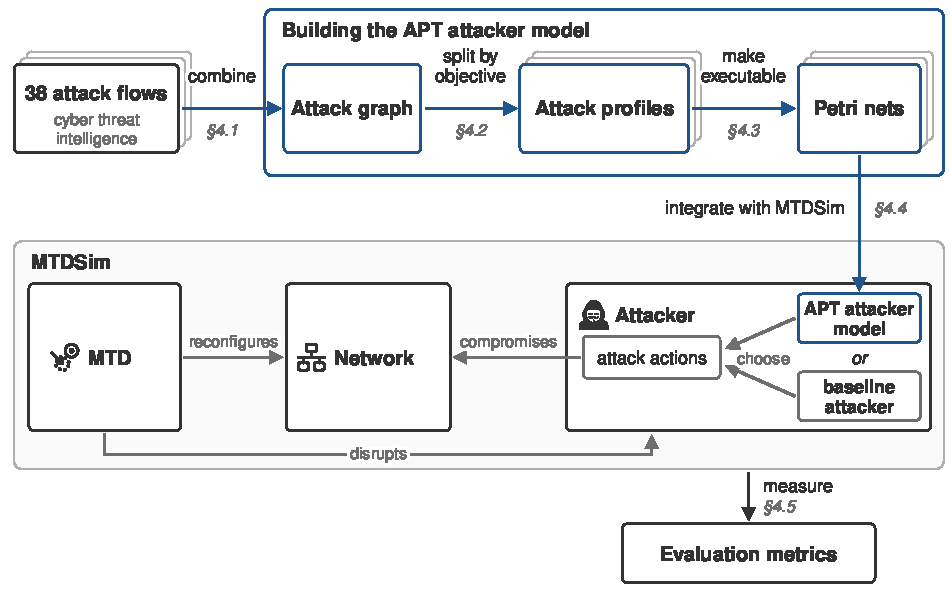
\includegraphics{fig_4-0a_method_overview}
  \caption[The pipeline that builds and runs the APT attacker model]{The
  pipeline that builds the APT attacker model from 38 attack flows and runs
  it in MTDSim. Blue marks what this dissertation builds.}
  \label{fig:pipeline}
\end{figure}

% ------------------------------------------------------------ preamble --
% The build told end-to-end, structure -> parameters -> execution.
% Selection discipline (Marc, 2026-08-12): relevant-and-interesting
% only --- the full implementation record stays in the repo's
% implementation docs, not the chapter.
%
% Chapter preamble (the former §4.2 section preamble, promoted
% 2026-09-04; unnumbered, a few sentences, no unit claim): the
% naming move --- "movement attacker" for the proposed model, "baseline
% attacker" for the inherited scripted attacker (V5: "the inherited
% non-APT baseline attacker") --- plus the one-sentence end-to-end
% orientation. No ladder re-narration; the chapter-opening figure owns
% the ladder.

% ---- Preamble: Marc's dictation (2026-08-19), passes 2-4 applied and his
%      3b walk ruled the same day (all markers resolved; P1/P2 from his
%      ruling dictation applied as live text). Rulings, do not re-flag:
%      "eight axes" (keep it simple --- no criterion/criteria discussion);
%      "we are going to" stays; "by the attacker model at runtime" stays;
%      no "successful"; "parsing and" removed; "attack profiles" (ratified
%      noun); "not touching" stays as sure; the "Any upgrades are in
%      Chapter 2" sentence CUT as a duplicate of "see Chapter 2"
%      (reversible); contractions stay (SUPERSEDED 2026-08-20: Marc's global
%      ruling --- contractions expand, everywhere). M2 withdrawn (input claim, not a
%      fidelity claim). Pass 5 (Marc) next: ~150 words against ~125; the
%      one duplicate pair is marked.
% ---- Pass 5 applied 2026-08-19 on Marc's "apply the table" ruling: the
%      four-slot grey box (bridge / naming pair / grounding + scope /
%      orientation), deletions and folds of his own words only. Seams
%      closed: (i) the ch2 apposition folded into the replacing sentence;
%      (ii) "beside" now carried once, in the scope sentence; (iii) the
%      traversing sentence joined to the execution clause with a colon
%      (cut: "--- the implementation of L0 to L4 in MTDSim", "This is").
%      Pre-pass-5 text in git history.
% ---- Threat-model framing RULED (Marc, 2026-08-20): option (a) --- the
%      identification sentence opens the preamble, from his dictation
%      (transcription-repaired: "we're terminate the" -> "we're terming it";
%      run-on split at the colon, clause order untouched); the section
%      heading stays "The movement attacker" (SUPERSEDED 2026-09-04: the
%      section is dissolved into the chapter and the name lives in the
%      prose; chapter title "APT attacker model"). Registry: threat model =
%      genre term / movement attacker = the name (terminology.md, ratified).
%      [3b minor] "tick off" is spoken register --- pass-6 candidate, your
%      call. [note] the next sentence also carries the axes + the naming
%      move --- one of the two naming clauses is a pass-5 cut candidate.
% ---- PASS 6 RUN AND RULED 2026-09-04 (voice-pass, split-stream WB + BB;
%      merged ledger in chat; Marc accepted all nine items). Restructured
%      as the CHAPTER preamble: two paragraphs, P1 the object and its
%      terms (pickup, naming pair, what "movement" means, the two
%      commitments), P2 the reader's map (spine sentence, figure, the
%      sub-question key). Applied: (1) opener re-nouned to parallel the
%      chapter title --- "The APT attacker model that we have produced,
%      which we are terming the movement attacker" (Marc's dictation;
%      terminology standardisation --- SUPERSEDES the 2026-08-20 "threat
%      model" opener; registry genre row amended, the thesis-wide
%      attacker-model row gains the data point); "motivated" is his verb;
%      (2) the L0--L4 glosses on the section key CUT (caption owns the
%      ladder), key by ordinal until ch1's contributions list fixes the
%      capture / model / evaluate labels; (3) the proof-of-concept
%      parenthesis CUT ("behavioural envelope", "declared policy" are repo
%      vocabulary, nowhere else in the tex); (4) "tick off" -> "meet";
%      (5) sentence-initial "And" dropped --- "This is built ... / This is
%      a proof ..." is the licensed two-beat pair; (6) "Two commitments
%      hold for the whole chapter" -> "Two commitments hold."; (7) the
%      proof-of-concept sentence in the hypothesis form ("built to test
%      whether ... not whether the model is true") --- SESSION WORDING,
%      accepted, Marc's re-dictation still welcome; (8) "the build that
%      answers them" -> "the pipeline that answers them"; (9) the
%      baseline appositive pared to "the scripted six-phase attacker
%      (Chapter 2)" ("inherited" is the registry's deprecated qualifier;
%      ch1 already glosses the inheritance). CUT with the restructure:
%      the second naming sentence ("Now that we have outlined the eight
%      axes ... we are calling it the movement attacker" --- duplicate of
%      the opener, back-reference a chapter away) and the three-stage
%      ladder sentence ("L0 to L2 are structure ..." --- competed with
%      capture / model / evaluate and placed execution outside the
%      chapter). Pre-pass-6 text in git history.
%      DO NOT RE-FLAG: "our existing simulator" (inside the ratified spine
%      sentence, Marc's hand only); "by the attacker model at runtime";
%      "in the real world"; the P2 opener's "it".
%      Handed to the integration check: fig:pipeline is a [p] float, so
%      the caption may name the movement attacker before the prose does.
%      Word count ~185 against the ~125--150 half-unit; the remainder sits
%      in ratified material (spine sentence, opener, commitments) ---
%      Marc's cut, if any.
% ---- PASS 6 ROUND 2 (2026-09-04): Marc's walk of the pass-6 text, his
%      dictation applied (repaired per pass 2+3a; "drops" -> "adopts" STT).
%      (a) \emph on "movement attacker" at its first fix (voice d: italics
%      introduce a term); the Section 3.3.4 pointer CUT --- the gap is the
%      section immediately before this chapter, and a pointer to 3.3.4
%      that itself points to 3.3.2 "makes no sense"; the 3.3.2 axes
%      pointer stays. (b) Replacement sentence re-dictated with the
%      movement attacker as subject, "inherited" restored in the
%      appositive by his dictation (the registry deprecates *inherited
%      attacker* as a NAME; as a description here it is his word), the
%      Petri net named in full ("more buzzwords": generalised stochastic
%      Petri net, the ratified L3 term). [3b] "aims to" now opens two
%      consecutive sentences (aims to meet / aims to replace) --- "replaces"
%      is the one-word alternative, your call. [3b] emphasis on "baseline
%      attacker" was a "maybe": NOT applied, because its first fix is ch2
%      §2.2.3 ("what we term the baseline attacker"); apply if wanted.
%      (c) "Two commitments hold." CUT (Marc: vacuous, inflated).
%      (d) The beside-MTDSim sentence re-dictated: "instrumenting our
%      existing attacker model with the movement attacker" is his frame;
%      "by construction" kept from the ratified text as the referent of
%      his "essentially" --- [3b] cut if not wanted. "This is" -> "It is"
%      (Marc: "This what is this"; the referent is the previous
%      sentence's subject). (e) Proof-of-concept sentence re-dictated:
%      "testing whether behavioural fidelity changes existing MTD
%      evaluation" (his words); the negative-scope tail "not whether the
%      model is true" KEPT --- it is the ceiling clause the cut §4.1
%      owed --- [3b] cut if his re-dictation was meant to replace it.
%      (f) P2 spine sentence split "with logic" into the three
%      sub-questions, each tagged SQ1 / SQ2 / SQ3 in a parenthesis; the
%      "Those are the three sub-questions of Chapter 1" sentence is
%      thereby absorbed; "structured representations" is his new noun
%      (parallels ch3 §3.1.3's attack-profiling definition). (g) The
%      section key now names the identifiers instead of ordinals.
%      SQ IDENTIFIERS (his ask): SQ1--SQ3 fixed at their definition site,
%      the ch1 sub-question sentence (three parenthetical labels inserted
%      there, minimal, ratify-on-read; the ch1 comment already reserved
%      the labels for that sentence). Convention note: with one research
%      question (architecture (a)) SQn is the fitting form; RQ1.1 would
%      imply several top-level questions.
%      3b WALK RULED (Marc, 2026-09-04, same day): "aims to replace" ->
%      "replaces"; \emph on "baseline attacker" APPLIED (his call, the
%      ch2 first fix notwithstanding); "by construction" CUT; the tail
%      "not whether the model is true" CUT (Marc: the X-not-Y form is not
%      his, and "the answer" was vacuous). No [3b] left open on this
%      preamble. Through pass 6; the integration check is next.
% [E2 SWEEP 2026-09-22 (register E2; Marc's ruling, spoken, the sweep
%  session): the naming clause "which we are terming the movement attacker"
%  DELETED --- the model is the APT attacker model, its chapter title, and no
%  naming sentence replaces it. The two later "movement attacker" in this
%  paragraph became "it". DRAFT STATE, ratify on read: the run of "It"
%  openers is the sweep's residue and is Marc's to reshape.]
% 2026-09-24 (Marc): "replaces" and "built beside" were both wrong --- the
% two are different attackers with different jobs (the baseline attacker
% is the reference); the relation is that MTDSim runs either under
% identical conditions, which is what makes SQ3's comparison controlled.
% "Instrumenting the baseline attacker with it" dropped. OPEN (flagged,
% not ruled): "and by the attacker model at runtime" reads circular inside
% the model's own introduction --- "the runtime loop" if that is the sense.
% [2026-09-04, Marc: the identifiers appeared twice in P2 and did not
%  read right] the section key FOLDED into the three spine clauses ---
%  each identifier once, paired with the sections that answer it; the
%  figure sentence closes the paragraph. Deletion and merge of the
%  ruled text only.
% [CONNECTIVE-PROSE PASS 2026-09-26, P1 ch4 opener] Roadmap re-keyed to
%  all five sections (4.5 was missing; the profiles moved to SQ1 as ch1's
%  contribution 1 has them; 'our defence mechanisms' dropped); the link
%  states ch3's finding instead of a third 'the gap motivated'; axes ->
%  properties (R4, Marc 2026-09-26); section-as-subject previews (R3); the
%  stray 'it' named; the ruled 2026-09-13 SIGNPOST SLOT landed in its own
%  words. The either-or sentence (2026-09-24) moved out: Figure 4.1's
%  caption and 4.4.1 carry it. SESSION-GENERATED on Marc's 2026-09-26
%  go-ahead (docs/workflows/connective_prose.md; audit
%  docs/implementation/connective_prose_audit.md); prior text in git.
%  RATIFIED 2026-09-26 (Marc: 'I accept all this').
% [CH3 REDRAFT ROUND 66, twin] the foothold claim retired with 3.4's (false since the baseline's persistence is full); now 3.4's gap sentence. Ratify on read.
% [PREAMBLE REWRITE 2026-10-03, Marc: "not written strongly ... the last two
%  sentences of the two paragraphs ... ruining the clarity"; one paragraph, as a
%  chapter preamble is] Gap -> model -> what it is -> map. Changes: the gap
%  stated as ch3's causal finding (ch3 l. "therefore remains unmeasured");
%  "aims to" -> "designed to"; "behavioural fidelity" (used nowhere else) ->
%  what is tested in plain terms; "in the real world" -> "from CTI" and "our
%  existing simulator" -> "MTDSim" (the wording of SQ1 and SQ2, overturning the
%  2026-09-04 do-not-re-flag on merit: the simulator is inherited, and CTI is
%  the source SQ1 names); each section pair now says what it produces;
%  "draws each step" CUT (a step is §4.5's defined term, one tactic executed);
%  the metrics' provenance stated (Table 4.3: nine of eleven cited); the
%  2026-09-13 SIGNPOST SLOT sentence ("Every assumption ... takes the model as
%  given") CUT --- §4.4's preamble now carries what Chapter 5 varies and what
%  it does not. DRAFT STATE, ratify on read; prior text in git.
% [ROUND 2, 2026-10-03, Marc: stealth and MTD awareness are scoped out, so
%  "the eight properties" overclaims; "nine of eleven" is nuance; the figure
%  sentence is vague] "six of the eight ... all but stealth and scheme
%  awareness" (apt_model_criterion.md: 5 and 8 NOT ADDRESSED, the rest
%  DESIGNED or DEMONSTRATED); "nine of the eleven" CUT; the figure sentence
%  CUT and the figure cited by the roadmap's lead sentence.
% [ROUND 3, 2026-10-03, Marc: claim the six strongly and answer the examiner's
%  "why not the other two"; no bracketed references (flow); SQ1--SQ3 treated
%  alike; subject first] The scope sentence gives the reason as a boundary:
%  both properties need MTDSim to change, and this dissertation changes the
%  attacker (exposure.py: the simulator offers "no detection model to be
%  stealthy against"; the join returns one failure verdict, so the attacker
%  cannot tell which mechanism deployed; ch7 future work lists both). The
%  figure leads the roadmap as its own subject-first sentence; each SQ is
%  named in the sentence that answers it.
% [ROUND 5, 2026-10-03, Marc: the limits read as "something bad" before the
%  reader meets the model; Figure 4.1 shows the pipeline, not the
%  sub-questions] The model is described first; the exclusion is one short
%  sentence after the scope sentence, without reasons (stealth's lives in
%  §4.5 and ch6, scheme awareness's in ch7). The figure sentence says what
%  the figure draws: the pipeline from the 38 attack flows to MTDSim, its
%  stages in section order. "Six of the eight" is design intent and holds
%  whichever way stealth is scored in ch6.
% [ROUND 4, 2026-10-03] CORRECTION of round 3: scheme awareness does NOT
%  need MTDSim to change --- the run wrapper already recovers the interrupting
%  mechanism's name (attacker.py InterruptSource: "record enrichment; neither
%  is read by the walk"), and the MTD interval is a run parameter. The
%  exclusion is scope (criterion axis 8: ruled out on timeframe; the
%  metric-manipulation route closed on evidence 2026-08-09). Stealth's reason
%  stands (Section 4.5: "MTDSim has no traffic and no detection mechanism").
%  No partial mark for scheme awareness: nothing the attacker decides reads the
%  mechanism or the timing. Stealth partial vs none: Marc's ruling, open.
% [ROUND 6, 2026-10-03, with the Figure 4.1 round] the figure sentence ends at
%  the pipeline: "the sections follow its stages in order" cut ("stage" is a
%  deprecated class noun for the parts, terminology row; the figure's
%  section labels and the next three sentences carry the order). DRAFT STATE.
The MTD evaluations surveyed in Chapter~\ref{ch:litreview} leave how MTD
performs against APT attackers unmeasured, because their attacker models lack
properties of an APT attacker. This chapter defines an APT attacker model
built to meet six of the eight properties of
Section~\ref{subsec:attacker-criterion}. It takes the same attack actions as
the baseline attacker, but the Petri net of its attack profile chooses its
next tactic at runtime. It is a proof of concept: it tests whether an attacker
that behaves like an APT changes what an MTD evaluation measures. Stealth and
scheme awareness, the other two properties, are left to future work.
Figure~\ref{fig:pipeline} shows the pipeline that builds the model from 38
attack flows and runs it in MTDSim. Sections~\ref{sec:technique-graph}
and~\ref{sec:attack-profiles} answer \ref{sq:capture}: they recover the
behaviour of APT attackers from CTI as an attack graph and four attack
profiles. Sections~\ref{sec:petri-formalism} and~\ref{sec:execution} answer
\ref{sq:model}: they execute each attack profile as a Petri net inside MTDSim.
Section~\ref{sec:evaluation-metrics} defines the metrics with which
Chapter~\ref{ch:experiments} answers \ref{sq:evaluate}.

% 1 unit (L0--L1). The campaign corpus and its snapshot; aggregating
% flows into tactic dependencies. Answers capture. Disclosures: what
% the graph cannot represent. (Consensus-thresholds disclosure removed
% per Marc's ruling, 2026-08-16 --- the lossless/views record lives in
% the repo, not the chapter.)
\section{Attack graph from attack flows}
\label{sec:technique-graph}
% [2026-10-03, Marc's ruling, round 2] Heading: "construction" was the vague
%  word; the heading names input and output, as "Attack profiles by
%  objective" names output and rule. AGGREGATE is the verb dissertation-wide
%  (overturns the morning's "combined": aggregate says the edges are counted;
%  ch1, Figure 4.1's label, Figure 4.2's caption and this section swept).
%  ATTACK FLOW verbatim dissertation-wide, never bare "flow" or "incident"
%  for one (ch3 defines it; ch3--ch5 and App. B captions swept; the App. B
%  tables and the Figure 4.2/4.4 generators still to sweep). DRAFT STATE.

% DRAFT STATE (2026-08-16): passes 1--5 COMPLETE; Marc signed the unit
% off at ~400 words (leave-and-forget until the next editing round).
% OPEN, recorded in the handoff: (a) the unit sits at ~1.6 ledger
% units --- a further cut or an explicit named overdraft at the ledger
% pass; (b) DISCHARGED 2026-08-20 --- app:cooccurrence is filled
% (Table~\ref{tab:preliminary-extraction}); its framing paragraph is the
% only prose still owed there, and the 80% CONFIRM is STRUCK, not
% resolved (see the note at the appendix chapter); (c) v19.1 pin still
% needs a home in sec:experimental-setup;
% (d) the cycles-preserved sentence was cut at pass 5 --- the L3 unit
% must now introduce loop preservation itself (readers default to
% assuming attack graphs are acyclic).
% FIGURE (2026-08-20, Marc's ruling): the three-panel figure that stood
% here is GONE --- it compressed 478 technique edges and 132 tactic
% transitions into two ~4 cm bands and read as a garble. The graphs it
% was trying to carry now live at full page size in app:full-graph,
% generated by tools/gap_appendix_figures.py; this unit keeps ONE
% parenthetical pointer, on the aggregation sentence. The two other
% panel refs were session-added parentheticals and are simply gone,
% restoring Marc's sentences as he wrote them.

% [CH4 SCRUTINY 2026-10-02, ledger S1, A1--A6 (handoff
%  2026-10-02_ch4_attacker_model_scrutiny.md), applied on Marc's accept-all.
%  S1: the definition opens the section. A1: CTID, the corpus and the case
%  against automated profiling are ch3 3.1.3's (l.~1520--1535), so the first
%  paragraph is cut to the corpus pointer; "MITRE Engenuity" (unsupported, X7)
%  and "spanning 2017 to 2024" (false: 2013--2025, X3) go with it. A2: the AND
%  point told once, in 4.3 (one token); fidelity vs coverage told once, with
%  Figure 4.2's own 39 %. A4: "skeleton of behaviour" cut. A5/A6: register;
%  "persistent across CTI" (uncited) re-based on the sentence before it.
%  Prior text in git (3f6b4f8c). DRAFT STATE --- ratify on read.]
% [CORPUS DISCLOSURE, Marc 2026-10-03: "hiding that sort of detail is
%  critical to a thesis like this" --- disclose, keep the example as the rule
%  picks it. 18 of 38 carry an ATT&CK group (data/gasp/classification.csv,
%  Table B-3a; Uber's G1004 audited high); criminal groups among them (G0102
%  Wizard Spider, G1016 FIN13, G1004 LAPSUS$); SearchAwesome Adware is adware.
%  Points to ch6 threats (its placeholder carries the line). OPEN for Marc:
%  the preamble and ch1 say "recover the behaviour of APT attackers from
%  CTI"; this sentence scopes it.]
% [§4.1 ROUND 2, Marc 2026-10-03: "on the right track"; one purpose per
%  paragraph: what the attack graph is; why attack flows; why tactics; the gap
%  before initial access. Checked: multi-tactic rule attack_stix.py:63 (20 of
%  124 techniques); same-tactic steps dropped where the graph is built (the
%  Figure 4.2 and App. B generators, petri/build.py:189); 88 % = 419/478,
%  39 % = 47/122, 10 of 38 from data/gap/gap_v0.5.json; the App. D table for
%  10/14/50 %; ATT&CK M1056 wording in
%  docs/sources/extractions/mitre_attack_precompromise.md. "Fidelity" and
%  "coverage" cut (each used in two senses); the Rodriguez precedent cut
%  (Marc: it carries no weight here; ch3 keeps the cite). DRAFT STATE.]
The attack graph aggregates the 38 attack flows into one weighted directed
graph whose nodes are the 15 tactics of ATT\&CK v19.1
\citep{mitre2026attackv19}. Each technique in an attack flow stands for its
tactic, and a technique listed under several tactics stands for the
leftmost of them in the ATT\&CK matrix. An edge runs from tactic $p$ to
tactic $q$ wherever an attack flow steps from a technique of $p$ to a
technique of $q$, and its weight is the number of attack flows that draw
it (Figure~\ref{fig:attack-graph-construction}). A step between two
techniques of the same tactic is not an edge: the time an attacker spends
within a tactic is its tactic duration (Section~\ref{subsec:dwell-times}).

% FIGURE (REBUILT 2026-10-03, Marc: the three-band version, with a second
% attack graph as a 15 x 15 grid, was "written off as confusing"). One worked
% example at the abstraction of Figures 2.1--2.3 and 4.1: part of two attack
% flows (chosen by rule: no technique edge in common, the most tactic edges in
% common; the excerpt has a step within one tactic), each technique in its
% tactic's band, aggregated; then the 88 %/39 % that section 4.1's choice of
% tactics rests on [bars CUT 2026-10-03: the prose says it]. The pair is
% drawn from the whole corpus; SearchAwesome Adware is not an APT, and 4.1
% says so (Marc: disclose, do not curate). Generated by
% tools/ch4_attack_graph_figure.py. DRAFT STATE --- ratify on read.
\begin{figure}[t]
  \centering
  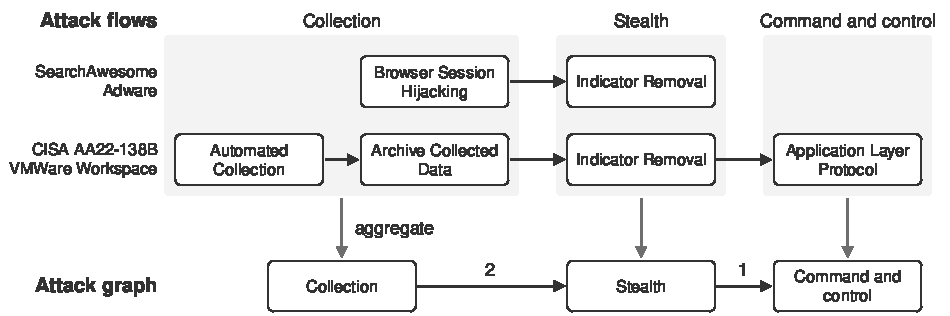
\includegraphics{fig_4-1a_attack_graph_construction}
  % [POLISH 2026-10-03, Marc: "what is the purpose of these patterns and
  %  colours ... they're supposed to be clear and intuitive". The dash is cut
  %  (the Collection band carries the step within one tactic); line width is
  %  the weight in every row; one arrow per tactic band down to its box. The
  %  caption no longer decodes marks. Round 2: 'aggregate' beside the arrows
  %  (in the gutter it read as a third attack flow); tactic boxes heavier and bold.
  %  [b]: Figure 4.1 takes the top of p. 17, so this one sits at its foot with
  %  text between, not stacked under 4.1 (the chapter page holds no top float).]
  % [ROUND 3, Marc 2026-10-04: "inconsistent design detracts from clarity
  %  unless motivated". One style, as Figure 4.1: the blue cut (4.1 spends blue
  %  on what this dissertation builds), the line width cut (it repeated the
  %  printed weight), the heavier bold tactic boxes cut (the row name says what
  %  they are). The caption's second sentence cut: it decoded marks, and the
  %  weight is defined in the paragraph that cites the figure. [b] -> [t]: the
  %  top of a page is the conventional place, and [b] was the thesis's only one.]
  \caption[How attack flows are aggregated into the attack graph]{Part of
  two attack flows aggregated into the attack graph.}
  \label{fig:attack-graph-construction}
\end{figure}

We built the attack graph from attack flows because they come from manual
attack profiling: an analyst drew the order of every step. We also tried
two automatic alternatives. Co-occurrence mining pairs techniques that the
same APT group or tool uses; keyword mining pairs a technique with each
technique its ATT\&CK description names. Neither pairing records which
technique came first, so both had to assume the order of the tactics. They
recovered 10\,\% and 14\,\% of the possible tactic-to-tactic edges, against
50\,\% for the attack flows (Appendix~\ref{app:cooccurrence}). The corpus
is not limited to APT attackers: 18 of the 38 attack flows are attributed to
a group in ATT\&CK, criminal groups among them, and the other 20 name no
group; one is an adware campaign. We keep all 38, because dropping the 20
would halve an already sparse corpus, so the attack graph records attackers
reported in CTI, not APT attackers alone (Section~\ref{sec:threats}).

We chose tactics as the nodes rather than techniques, trading resolution
for edges that recur across attack flows. Most edges between techniques
come from one attack flow alone: 88\,\%, against 39\,\% of the edges
between tactics (Appendix~\ref{app:full-graph}). An edge
weight needs several attack flows behind it, because
Section~\ref{sec:petri-formalism} turns the weights into the probability of
each next tactic. Tactics also make the tactic-to-action mapping smaller: it maps 15 tactics,
rather than the 124 techniques the attack flows use, to MTDSim's six attack
actions (Section~\ref{sec:execution}).

The attack graph is sparsest before initial access: reconnaissance appears
in 10 of the 38 attack flows. Reconnaissance and resource development
happen largely outside the scope of the defender's controls
\citep{mitre2026attackkb}, so the investigations that CTI reports rarely
see them, and any CTI corpus shares the gap. An MTD evaluation cannot
ignore it, because shuffling works by making the attacker's reconnaissance
out of date. Section~\ref{sec:petri-formalism} adds the missing edges as
the pre-intrusion overlay.
% [2026-10-03: the 2026-08-16 ruling below is REOPENED on merit by Marc's
%  round 2 --- the shuffling sentence is the defender-side reason, in ch2's terms.]
% [RULED (Marc, 2026-08-16), do not re-flag: the defender-validity
%  sentence and the observability-boundary naming stay OUT --- the "so
%  what" is the synthetic pre-intrusion structure, the L3 unit's
%  disclosure; if the term is wanted, L3 or ch6 coins it.]

% 1 unit (L2). Objective over motivation; the four classes. Answers
% capture. Disclosures: what the partition produced, operator
% concentration.
\section{Attack profiles by objective}
\label{sec:attack-profiles}

% [§4.2 REDRAFT, Marc 2026-10-04: "I cannot decipher it"; the examiner's
%  questions are why split, what are the four, why four (not more, not
%  fewer), where positioning went, how the profiles differ. One purpose per
%  paragraph: why split; the four attack profiles; why the sources decide;
%  what the profiles change. RULED that day: plain "objective" (3.1.1's
%  definition); the profiles are $c_1$ to $c_4$ only, defined once in
%  Table 4.1 ("double extortion" and the other names CUT: the Mac crypto
%  stealer is not double extortion, and a name is one more term); the
%  motivation paragraph CUT (nobody has asked; App. B.3 row 1 keeps it); the
%  Wizard Spider check CUT (the ATT&CK group page was one of the sources the
%  classification read, so groups landing in one profile is partly by
%  construction). "Four after one attack flow per APT group" CUT here:
%  Section 4.3 states the rule where it applies. Checked: the 19/7/7/5 split
%  and the three adjudicated flows from data/gasp/metadata_audit.csv; 19/38
%  and 14 from Table B.3 (tools/gasp_partition_candidates.py); the reach
%  counts in paragraph 4 from data/gap/gap_v0.5.json under the audit
%  classes (execution 13/19, 7/7, 7/7, 5/5; stealth 16/19, 5/7, 5/7, 4/5;
%  command and control 17/19, 6/7, 5/7, 4/5; collection 14/19, 1/7, 1/7,
%  2/5; c3 reaches exfiltration in 3/7); positioning never entering
%  stages 4--5 from docs/sources/extractions/alshamrani2019.md.
%  ROUND 2 (same day, after the Figure 4.3 cold reads): paragraph 3 ties the
%  figure's objective cells to the text (c1 10/19, c3 3/7 against sources
%  that all report the theft; Muddy Water's zero-confidence encryption step,
%  per_flow_justifications.md); paragraph 4 states its rule (more than half
%  of every profile: execution, stealth, discovery, command and control;
%  "execution, stealth and C2" alone read as cherry-picked) and says the
%  objective rows differ by the classification's design. Prior text in git
%  (39544a76, 0847a5dc).
%  ROUND 3 (Marc, same day: naming c1 "exfiltration" when 9 of its 19 attack
%  flows never draw the exfiltration tactic, and one draws impact, borrows
%  ATT&CK's term "in this cheeky way"): Table 4.1 and the figure headers now
%  say what the SOURCES report the attacker did (stole data, impeded systems,
%  both, neither); ATT&CK's tactic names appear only as tactics, the rows of
%  Figure 4.3. "Impeded systems" = encrypted, destroyed or hijacked them
%  (paragraph 2); hijacking is ATT&CK's resource hijacking, under impact.
%  DRAFT STATE --- ratify on read.]
% [4.2 ROUND 4, 2026-10-04, Marc: "lots of facts ... lots of jumping"; the
%  text had gone stale under the new labels. One job per paragraph: why split
%  (P1); the two questions and the four profiles they give (P2); where the
%  answers come from (P3); what Figure 4.3 shows (P4); what the split changes
%  (P5). "mix" -> the attack graph pools the 38 attack flows, so its weights
%  average over objectives. The four profiles are now the answers to two
%  yes-or-no questions (Table 4.1 and the Figure 4.3 header rows), so no label
%  has to stand on the others ("both", "neither" CUT: Marc, c3 cannot be named
%  without c1 and c2); this also answers "why four" (two questions, two answers
%  each). The mapping from 3.1.1's objectives is stated (two are reached in
%  actions on objectives); c4 said as it is (three evicted, one positioning,
%  one adware: metadata_audit.csv), so "positioning and eviction look alike"
%  CUT. CUT as stale or off-purpose: the ATT&CK-recording sentence, the
%  terminal-tactic disagreement (19 of 38, 14; Appendix B.3 keeps it), Muddy
%  Water's zero-confidence step (no longer a stand-out once c1 is "stole
%  data"). The last line now says how 5.4.1 tests the partition. DRAFT STATE,
%  ratify on read.]
% [4.2 ROUND 5, 2026-10-04, Marc's line flags: "pools" then "average" (one
%  word: averages); "groups" -> classify / class; "each of these four attack
%  graphs is an attack profile" (said once, in the definition); why two
%  questions and not three (positioning never reaches actions on objectives,
%  3.1.1, so it is the no/no answer: no third question, no eight profiles);
%  "the two answers" -> their yes-or-no answers; c4 said as the catch-all it
%  is; "partitions by motivation or APT group" CUT ("answering a question
%  nobody's asking"; Appendix B.3 now unreferenced from the body, flagged).
%  P3: the sources named (CTID description + ATT&CK group page or the cited
%  threat report: metadata_audit.csv source_used, every row); the limitation
%  said as one. P4: preparation CUT (4.1 says it; the figure shows it); the
%  colon that restated its own clause CUT; the objective rows described as
%  they are drawn. P5: 5.4.1 said as what it does. DRAFT STATE, ratify on
%  read.]
APT attackers with different objectives act differently after the foothold
(Section~\ref{subsec:apt}). The attack graph of
% [ROUND 6, 2026-10-04, clarity pass (Marc: "90% of the way there"): "class"
%  and "in the same way" CUT (extraneous terms); an attack profile is said as
%  what it is, a subgraph of the attack graph with its own weights; P2 leads
%  with the three objectives and says why positioning gets no question (it has
%  no action of its own); P3 says the routine once and the three decisions
%  once; "not a reliable answer" (rhetorical) -> what the attack flow lacks;
%  "turns ... into" -> formalises; "removes the split" -> ablates. DRAFT STATE.]
Section~\ref{sec:technique-graph} is built from all 38 attack flows, so it
averages the behaviour of attackers with different objectives. We therefore
split it by objective into four attack profiles, $c_1$ to $c_4$. Each attack
profile is a subgraph of the attack graph, aggregated from its own attack
flows only.

Section~\ref{subsec:apt} gives three objectives. Data exfiltration and
impediment each have an action in actions on objectives: the attacker steals
data, or it impedes the victim's systems by encrypting, destroying or
hijacking them. Positioning for future operations has no action of its own,
because the attacker stays in post-intrusion operations. We therefore asked
two questions of each attack flow: did the attacker steal data, and did it
impede the victim's systems? Their yes-or-no answers give
the four attack profiles of Table~\ref{tab:attack-profiles}. An attack flow
that did both belongs to $c_3$ alone, so no edge weight counts it twice.
Six of the seven attack flows of $c_3$ are ransomware that stole data and
then encrypted the systems. The five attack flows of $c_4$ did neither,
whatever the reason: three attackers were removed from the network before
they acted, one positioned for future operations, and one ran an adware
campaign.

\begin{table}[ht]
  % [ht]: at [t] it floated above the section heading of 4.2.
  \centering
  \caption[The four attack profiles]{The four attack profiles.}
  \label{tab:attack-profiles}
  \tablestyle
  \begin{tabular}{@{}lccrl@{}}
    \toprule
    Attack profile & Stole data & Impeded systems & Attack flows & Example \\
    \midrule
    $c_1$ & yes & no  & 19 & SolarWinds \\
    $c_2$ & no  & yes &  7 & NotPetya \\
    $c_3$ & yes & yes &  7 & Conti Ransomware \\
    $c_4$ & no  & no  &  5 & Hancitor DLL \\
    \bottomrule
  \end{tabular}
\end{table}

We answered both questions from the CTID description of each attack flow
and, where that was not enough, its ATT\&CK group page or the threat report
it cites. Three attack flows stayed open after these sources, and we decided
them ourselves (Appendix~\ref{app:classification-audit}). We did not read the
answers off the attack flow, because its analyst drew only the steps the
threat report describes, and these can stop short of the objective. Only 10
of the 19
attack flows of $c_1$ reach the exfiltration tactic, although the sources of
all 19 report the theft (Figure~\ref{fig:attack-profiles}).

% FIGURE (REBUILT 2026-10-04, Marc: the grids were "decoration ... I don't
% know what the blue columning does"; a bar-chart mock was "a lot of numbers
% ... not a natural viewing state"). Takeaways first: the profiles share the
% tactics through the middle of an attack, differ at the objective, and are
% all sparse before initial access. One row per tactic in ATT&CK order, one
% column per attack profile; a ring is the whole profile, the disc's area the
% share of its attack flows that reach the tactic (Wilke 2019, ch. 17;
% sec. 6.1 for the horizontal names). Gaps: after resource development (the
% PRE-ATT&CK tactics until v8) and before the two tactics Table 4.1
% classifies by [REPLACED same day, Marc: the rows are grouped by the four
% lifecycle stages of the failure matrix, in the controller-mapping figure's
% band style, so the takeaways are the stages; the key is five discs
% labelled at the ends (a continuous scale, not bins); no key title and no
% sizes in the headers (the caption and Table 4.1 carry them)]. Two cold
% reads (a CS student, a visualisation critique) and a third on the
% shade-versus-disc choice; the disc won (1/19 is visible, and none is an
% empty ring). Greys only. The grids moved to Appendix B.
% Generated by tools/ch4_profile_reach_figure.py. DRAFT STATE --- ratify on read.
\begin{figure}[t]
  \centering
  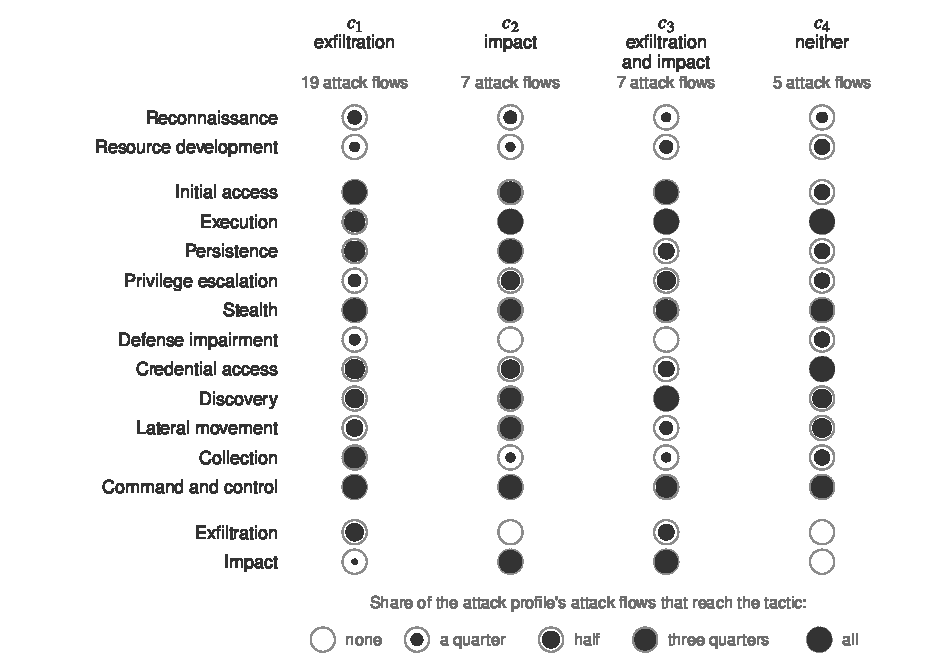
\includegraphics{fig_4-2b_profile_reach}
  \caption[The tactics each attack profile reaches]{The share of the
  attack flows of each attack profile (Table~\ref{tab:attack-profiles}) that
  reach each tactic.}
  \label{fig:attack-profiles}
\end{figure}

% [2026-10-04: the stages now defined in 3.1.1 (was a forward reference to
%  4.4.4); "objective" -> "actions on objectives" (Marc's ruling). DRAFT STATE.]
Figure~\ref{fig:attack-profiles} groups the tactics by the four stages of
Section~\ref{subsec:apt}. Before actions on objectives, the attack profiles
share their most common tactics: execution, stealth, discovery and command
and control appear in more than half the attack flows of every attack
profile. The attack profiles differ in actions on objectives. No attack flow
of $c_2$ or $c_4$ reaches exfiltration, and none of $c_4$ reaches impact.
Collection, which neither question asks about, appears in 14 of the 19
attack flows of $c_1$ but in only one each of $c_2$ and $c_3$.

Section~\ref{sec:petri-formalism} formalises each attack profile as a Petri
net, whose attacker chooses its next tactic only among the edges its attack
flows drew. Two attack profiles that reach the same tactics can
therefore move between them differently (Appendix~\ref{app:profile-edges}).
Section~\ref{subsec:ablation-attack-profiles} ablates the split: it runs the
APT attacker model on the whole attack graph of
Section~\ref{sec:technique-graph} and compares the results with those of the
four attack profiles.

% 1 unit (L3). The formalism, the alternatives ranked in a sentence each
% (a feasibility study sits behind the choice; single-token walk over
% per-objective net structure). Answers model, with the next one.
% "generalised", never "general". Disclosures: synthetic pre-intrusion
% structure (the corpus begins at initial access), entry-point selection
% (D8: both *testable* --- the initial-access seed is a toggle, no
% published run; scan 2026-08-17). RULED OUT (Marc, 2026-08-17): the
% executed-not-solved / CTMC closed-form vocabulary and the standalone
% analytical track are not wanted in the chapter --- the record holds
% them (stochastic_timing_design.md §1).

\section{Petri-net formalism}
\label{sec:petri-formalism}

% [REDRAFT 2026-10-04, Marc: "I'm just generally lost when I'm reading this";
%  the supervisor accepted the formalism on 2026-09-22 (register E9) and left
%  the notation to be simplified to the standard symbols. Rules applied, each
%  sourced: Halmos 1970 s15 ("the best notation is no notation"; no symbol
%  used once), Knuth et al. 1989 rules 2, 11, 13--15 (no sentence opens on a
%  symbol; define twice, in words and in symbols; prose readable with the
%  formulas skipped; one notation per thing; no needless subscripts), the
%  genre's own order (Bland 2020 after Murata: standard tuple, then the
%  instance as a where-list, then the extension as a larger tuple).
%  OVERTURNED on merit, Marc to confirm:
%   * P1's elimination argument (SPN times every transition, DSPN adds a fixed
%     delay, a DAG cannot hold the cycles; 2026-08-18 rulings): the choice is
%     the field's convention, and is now said so, with the positive reason.
%   * the 7-tuple with T_T, T_I -> the standard 6-tuple (E9); the instance no
%     longer re-subscripts the tuple (P_c, W_c): c is fixed, said once.
%   * w_c(p,q) -> W(t_pq), and |A_c(p->q)| -> the count n(p,q): one weight
%     symbol, not two; F_v, V, F_success, F_none -> F alone (success and no
%     verdict both use the base weights, so the family carried two all-ones
%     members); sigma -> "one-tenth" (never used in a formula); "vanishing",
%     "tangible", "verdict-conditioned" cut (nothing later uses them).
%   * the notation table (tab:gspn-notation) cut: every symbol is now defined
%     in one list in one section, and Figure 4.4 draws them.
%  KEPT, ratified: the zero-factor sentence (2026-09-08), the success-needs-no-
%  factor sentence (A4), the join paragraph (2026-09-26, symbols updated).
%  Prior text and its ruling comments: git ac2dd7c4. DRAFT STATE.]
% [ROUND 2, 2026-10-04 (Marc: "100 percent on the right track"; line flags
%  applied): P1's last sentence split, subject first, and a signpost to the one
%  extension; W said plainly, the rate defined with the delay; "by the same
%  construction" -> what depends on c; "carry weight" -> "rest on 29 of the 38";
%  one token folded into M_0 with its consequence; the 4.1 sparsity restatement
%  cut (4.1 says it and points here); the overlay's guard said as it is (no
%  attack flow of c3 or c4 leads on from reconnaissance); "the base weights
%  stand" -> "keep their base weights"; "succeeded" -> "completed" (c4's evicted
%  attackers completed every step they drew); the join paragraph reframed as
%  what the Petri net still lacks, which defines the join; Figure 4.4 (b) and (c)
%  worked into the text. DRAFT STATE.]
% [ROUND 4, 2026-10-04 (Marc: "90% of the way ... that little clarity touch"):
%  a sentence pass on Gopen & Swan 1990 (subject next to its verb; one stress
%  candidate per sentence, the new point at its end) and Knuth et al. 1989
%  rule 2 (no sentence opens on a symbol): P1's first sentence split (two
%  points); the token's job its own sentence; the firing rule two sentences;
%  "whose rate" disambiguated; list items open on words; the overlay named,
%  then listed; "which returns failure" disambiguated. The extension is the
%  larger tuple, the genre's convention (Bland 2020: PNPSC = the standard
%  tuple plus new elements). The bridge paragraph is cut: the 4.4 preamble,
%  next, says the same. DRAFT STATE.]
Stochastic Petri nets are an established formalism in MTD evaluation
\citep{chobenasher2018, mendonca2023}. Cai et al.\ compare MTD techniques
with one variant in particular, the generalised stochastic Petri net (GSPN)
\citep{cai2016}. We follow this convention and formalise each attack profile
as a GSPN. An attack profile gives only the edges between tactics and their
weights. A GSPN adds a token and two kinds of transition. The token marks the
tactic the attacker is on. A timed transition models the time the attacker
spends on a tactic, and an immediate transition models its choice of the next
tactic.

A GSPN is a directed bipartite graph of places and transitions
\citep{marsan1984}. Tokens sit on places. A transition is enabled when each of
its input places holds a token. Firing it moves a token from each input place
to each output place. A \emph{timed} transition fires after a delay drawn
from an exponential distribution; its \emph{rate} is one over the mean delay.
An \emph{immediate} transition fires in zero time and takes priority over
timed ones. Of several enabled immediate transitions, one fires, with
probability proportional to its weight. Following Ajmone Marsan et al.\ \citep{marsan1995}, a GSPN is the tuple
\begin{equation}
  \mathcal{N} = (P, T, I, O, W, M_0),
  \label{eq:gspn}
\end{equation}
where $P$ is the set of places; $T$ the set of transitions, each timed or
immediate; $I$ and $O$ the input and output arcs; $W$ the rate of each timed
transition and the weight of each immediate one; and $M_0$ the initial
marking, the number of tokens on each place. The full definition adds
inhibitor arcs and priority levels, which this dissertation does not use.

Each attack profile $c$ (Section~\ref{sec:attack-profiles}) gives a Petri
net $\mathcal{N}_c$, built as follows. Only its places and weights depend on
$c$. Figure~\ref{fig:gspn-gadget}(a) draws the construction for one tactic
$p$.
\begin{description}[nosep, leftmargin=1em]
  \item[Places $P$:] one place $p$ for each tactic of the attack profile and,
  for each, a decision place $\hat{p}$ at which the next tactic is chosen.
  \item[Transitions $T$:] a timed transition $\tau_p$ from each tactic $p$
  to its decision place $\hat{p}$, whose firing is the attacker carrying out
  the tactic; and an immediate transition $t_{pq}$ from $\hat{p}$ to $q$ for
  each edge $p \to q$ of the attack profile with a base weight above zero
  (Equation~\ref{eq:base-weight}). No transition leads from a tactic back to
  itself: the time spent in a tactic is the delay of $\tau_p$.
  \item[Arcs $I$, $O$:] those of the chain
  $p \to \tau_p \to \hat{p} \to t_{pq} \to q$.
  \item[Weights $W$:] each timed transition has rate
  $W(\tau_p) = 1/\mu_p$, so that its delay has mean $\mu_p$, the mean duration
  of tactic $p$ (Section~\ref{subsec:dwell-times}). Resource development has
  a mean duration of zero, so its transition is immediate. Each immediate
  transition has the \emph{base weight} of its edge $p \to q$, the share of
  the attack profile's attack flows leaving $p$ that go to $q$:
  \begin{equation}
    W(t_{pq}) = \frac{n(p, q)}{\sum_{q'} n(p, q')},
    \label{eq:base-weight}
  \end{equation}
  where $n(p, q)$ is the number of the attack profile's attack flows that
  draw $p \to q$. The base weights count each APT group once, through its
  attack flow with the most steps, so that a group reported several times
  does not outweigh the rest. They rest on 29 of the 38 attack flows.
  \item[Initial marking $M_0$:] one token on reconnaissance. The single token
  means the attacker pursues one line of the campaign at a time: where an
  attack flow draws parallel branches, the token follows one of them.
\end{description}

In $c_3$ and $c_4$, no attack flow leads on from reconnaissance, so the token
could not leave the place it starts on. For these two attack profiles we add
the \emph{pre-intrusion overlay}. It consists of three immediate transitions
that none of their attack flows draws: from reconnaissance to resource development, from
resource development to initial access, and from initial access back to
reconnaissance, for an attacker whose intrusion fails. Their weights are
declared. A place with no transition of its own sends all its weight through
the overlay. A place with transitions of its own gives the overlay transition
one-tenth of its weight, and its own transitions share the other nine-tenths
in their proportions.

% [ROUND 3, 2026-10-04 (Marc: "one extension is the verdict ... an extension
%  for the sake of an extension"; "the motivation isn't there"): the why first,
%  in its own paragraph (attack actions fail; the base weights describe
%  success; a GSPN cannot read a verdict from outside the net), then the
%  extension as one added element of the formalism, displayed as the pair
%  (inherit, then extend: Bland's PNPSC convention), then the rule. The P1
%  announcement is cut: it made the extension read as part of the GSPN, and it
%  named Ajmone Marsan twice. The failure causes stay in 4.4.1. DRAFT STATE.]
Each attack action the APT attacker model runs in MTDSim succeeds or fails;
this outcome is the attack action's \emph{verdict}
(Section~\ref{subsec:runtime-mechanics}). The base weights describe where an
attacker goes after a success, because an attack flow draws only the steps
its attacker completed (Section~\ref{subsec:failure-matrix}). Routed on them
alone, an attacker that fails would carry on as though it had succeeded. A
GSPN cannot route on the verdict: its weights are constants, or functions of
the marking, and the verdict comes from MTDSim, outside the Petri net.

We therefore extend the GSPN with one element, the failure matrix $F$: a
declared factor between zero and one for each pair of tactics
(Section~\ref{subsec:failure-matrix}). The Petri net of attack profile $c$
becomes the tuple
\begin{equation}
  (P, T, I, O, W, M_0, F),
  \label{eq:vc-net}
\end{equation}
whose first six elements are those of $\mathcal{N}_c$.
When $\tau_p$ fires and its attack action fails, $F$ scales the weights of
the immediate transitions out of $\hat{p}$:
\begin{equation}
  W(t_{pq} \mid \text{failure}) =
  \frac{W(t_{pq})\, F(p, q)}{\sum_{q'} W(t_{pq'})\, F(p, q')}.
  \label{eq:routing}
\end{equation}
After a success, or at a tactic that dispatches no attack action, the
immediate transitions keep their base weights. A factor of zero disables a
transition for that firing only; places, transitions and arcs never change.
An MTD deployment can also cut a timed transition short; if an attack action
was in flight, its verdict is failure (Section~\ref{subsec:runtime-mechanics}). Figure~\ref{fig:gspn-gadget}(b)
gives both sets of weights at initial access in $c_1$.

% [BRIDGE paragraph CUT in round 4 (Marc: "that reads like it's going to be
%  the 4.4 preamble, which is literally next"). Prior text in git c25d05a5.]

% FIGURE fig:gspn-gadget --- generated by tools/gspn_gadget_figure.py from the
% c1 routing net (primary corpus variant, overlay as run), the v4_failure_only
% failure matrix composed by the controller's own compose(),
% tactic_durations.json and the pinned bundle. Marsan's drawing convention,
% legend inside the figure. Regenerate, never hand-edit. 2026-10-04: symbols
% to the redraft (W, no w_c / W_c), panel titles to c_1 (was "the exfiltration
% profile", stale since the 4.2 relabel), "gadget" off the panels. Round 3
% (Marc: the foothold contrast "is more of a nuanced point"): panel (c) off,
% one worked tactic; the caption says what to look at. DRAFT STATE.
\begin{figure}[tbp]
  \centering
  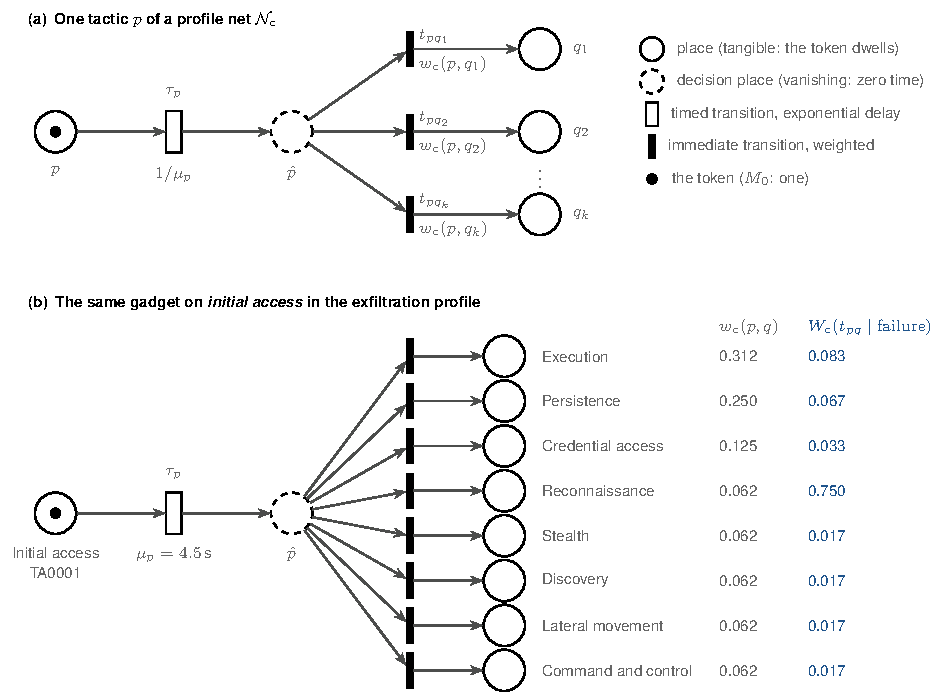
\includegraphics{fig_4-3a_gspn_gadget}
  \caption[One tactic of a Petri net]{One tactic of a Petri net. (a)~The
  construction for one tactic $p$, with the legend for every mark.
  (b)~Initial access in $c_1$: each successor $q$ with its base weight
  $W(t_{pq})$ and, in blue, its weight after a failure,
  $W(t_{pq} \mid \text{failure})$ (Equations~\ref{eq:base-weight}
  and~\ref{eq:routing}). After a failure, most of the weight moves to
  reconnaissance.}
  \label{fig:gspn-gadget}
\end{figure}


% ---- PASS 5 APPLIED 2026-09-08 (split-stream: white box + black box, merged;
%      Marc's rulings in chat the same day). Design record: git history of
%      docs/handoffs/2026-09-08_ch4_s44_structure.md (deleted in the shipping
%      commit, per the handoff lifecycle). Pre-restructure text: git 9a333c48.
% RULED (Marc, 2026-09-08):
%   * Title: "L4: Joining the profile net to MTDSim" (was "The attacker-agent
%     traversal in MTDSim" --- named the run, not the join).
%   * Four units under the section, front-loaded: the runtime mechanics
%     (the join, held fixed), then one unit per declared input --- the three
%     components of the controller layer that join the attack profiles to
%     MTDSim, each swept in the sensitivity analysis. "The controller layer"
%     retired as a heading (it does not make sense until the section has
%     been read); the layer is named in the preamble.
%   * FRONT-LOAD, POINT FORWARD: §4.4 states what the model runs with; the
%     why-this-shape and what-bounds detail lives in the appendices and the
%     sensitivity analysis (sec:sensitivity, ch5 "Experiments" once the
%     experimental-setup/results merge lands), forward-referenced from each
%     unit. Cut on that ruling: the derivation-tier sentence (App. B.4 carries
%     the tiers row by row); the kernel-value, floor and reconnaissance-to-
%     impact sentences (App. B.6 declares gamma, delta, z; ch5 sweeps them);
%     the overfit-concern and "they can be justified" sentences.
%   * Join material first: the runtime loop, the verdict, the clock, the
%     retrace, the penalty, the ceiling --- every symbol defined before use.
%   * The convergent cuts: the loop-as-prose paragraph (fig:runtime-loop and
%     §4.3's routing sentence carry it), the Eq. 4.4 restatement (S68/S69 ---
%     S69 was the 2026-08-20 one-arm seam repair; its content moved to §4.3
%     on 2026-09-08, Marc's eye), the mutation example in the opener (§4.3
%     "cut short by an MTD mutation" carries it), the flourishes.
%   * Twelve symbol bindings to §4.3's notation table (mu_p, phi, F_failure,
%     v, none, w_c, R, d, tau_p) --- one clause each, nothing else inserted.
%   * Table 4.2 to one panel, tactic and mean dwell only (families, badges,
%     multipliers to App. B.4 --- "this is what we are rolling with").
%   * stage/phase: "stage" = the four lifecycle consensus stages (s(.),
%     Delta); "phase" reserved for the baseline attacker's six. Registry row
%     added.
%   * Rejected (do not re-flag): re-opening the 2026-08-20 rulings (the
%     zero-or-one constraint sentence, the 45.0 s / 0 s worked examples, the
%     three-citation sentence); the "kernel vs floor tension" (verified
%     false: gamma^2 = 0.0625 < z = 0.1 is what zeroes the Delta = 3 cell);
%     nu as a symbol (no second use); the closed-world clause to §4.3.
% SESSION GLUE, flagged [3b] for Marc: the preamble's last sentence (his
%   chat words + the sweep pointer) and one forward-pointer clause per
%   declared-input unit ("just put a forward pointer if you need").
% LEDGER: ≈ 1000 words on four headings; two units + the chapter's slack
%   fund three, one unit of overdraft claimed on the writing-guide ledger
%   (both streams measured ≈ 850--900 as the floor at this shape).
% MUST-CARRIES kept: the ceiling paragraph (the mapping as chosen input);
%   the two [prose slot --- Marc] caveats beside the floats.
\section{Integration with MTDSim}
\label{sec:execution}
% [STRUCTURE 2026-10-04: subsec:runtime-mechanics now labels this section
%  (the runtime loop subsection is folded into it); every reference reads
%  "Section 4.4".]
\label{subsec:runtime-mechanics}

% [PREAMBLE REDRAFT 2026-10-04 (Marc: "I'm just completely lost by the structure";
%  "there's no rhyme or reason to these sentences"; his dictation kept where it
%  works). Four jobs, in the order an examiner expects of a section opener that
%  carries its headline figure: why the section exists (P1), the figure and its
%  walkthrough (P2), what the overview guarantees and its limit (P3), the map
%  to the subsections and the standard each meets (P4, with the four bases).
%  Moved out: the dwell-only clause of step 2 (4.4.2 says it); the dead end to
%  4.4.3, beside the stall (Marc: an implementation detail); "the one time the
%  Petri net does not supply" to 4.4.1 (a timing fact). Repaired: "the six
%  attack actions ... held identical for both attackers" overstated it (the
%  vulnerability memory is the APT attacker model's only, Marc 2026-09-28, and
%  the drawn dwell replaces an attack action's own cost), so P3 says the attack
%  actions are shared and names the two declared changes; step 5's "the base
%  weights stand" -> 4.3's "keep their base weights". Prior text and its
%  ruling comments: git 3ce6e0b5, and the history block below. DRAFT STATE.]
% [ROUND 4, 2026-10-04 (Marc: the opening contrast "seems cliche"; "act on the
%  network" vague; "ordered procedure" not the term; "the next choice" of what):
%  the point first; the attack actions named as Section 2.2.3 lists them; the
%  baseline's "fixed procedure" (2.2.3's term); the choice named. DRAFT STATE.]
% [ROUND 5, 2026-10-04 (Marc: round 4's P1 "bombarding them with different
%  terminologies that don't tie into anywhere"; "the loop" vague; "what's the
%  order"; the fixed procedure "what?"; "sets the weights, is that right?"; the
%  cut contrast "was also the motivation"): three ideas only, each in a term
%  Section 4.3 or 2.2.3 defined (tactic, attack action, verdict, token,
%  immediate transitions). The motivation back, plainly; the attack-action list
%  and the fixed procedure cut (the chapter opener says the model takes the
%  baseline attacker's attack actions); the loop defined where it is named;
%  "selects" because a success keeps the base weights. DRAFT STATE.]
The Petri net of an attack profile chooses the attacker's next tactic, but it
cannot carry the tactic out. MTDSim's attack actions carry tactics out on the
network, and each returns a verdict. The APT attacker model integrates the two
in one loop: the tactic the token reaches runs as one of MTDSim's attack
actions, and the attack action's verdict selects the weights of the immediate
transitions that take the token to the next tactic.

% FIGURE (2026-10-04): fig:runtime-loop REBUILT as section 4.4's headline (Marc:
% section 4.4 is Figure 4.1's "integrate with MTDSim" arrow enlarged, so it is a
% sub-model diagram in Figure 4.1's boxes; "the big point of this is the arrows
% and the numbering"). Generated by tools/runtime_loop_figure.py (SVG, Chromium
% print, at \textwidth; the sibling of fig:pipeline, whose style and icons it
% imports). The Petri net in Figure 4.4's marks, with a key; the three declared
% inputs as boxes named and numbered as their subsections; MTDSim as Figure 2.1
% draws it, the vulnerability memory in the Attacker. Blue outlines mark what
% this dissertation builds, as Figure 4.1. Cut: the glyphs (thumbnails of
% Figure 4.6, Table 4.x and Appendix B), the band labels, "one Petri net, a
% fragment", the clock. Prior drawing and caption in git (c25d05a5).
% ROUND 2 (Marc, same day: "visually overwhelming"; "not really aligned"):
% one grid, two lanes, straight arrows, the key cut (Figure 4.4 carries it;
% the caption points there), ~20 per cent shorter.
% ROUND 3 (Marc: "we're tracking dark blue, black and dark grey"; three
% meanings for arrows): blue is the loop and nothing else; boxes in ink;
% two arrow kinds (the loop, the net's arcs); MTDSim's couplings not drawn
% (Figure 4.1's); step 5 back to the decision place; step 6 on its arc.
% ROUND 4 (Marc: F is in the formal definition, so why outside the net?):
% the dwell times (W's rates) and the failure matrix (F) drawn inside the
% Petri net under what they set; the mapping alone outside; MTDSim's
% modules share a top and a bottom, their rows aligned.
% ROUND 5 (Marc: the failure matrix reweights the immediate transitions):
% step 5 straight up into them; the success arm and junction dots cut (a
% success changes no weight; the caption says so); frame titles on the
% border; MTDSim compressed.
% ROUND 6 (Marc: "what happened to the success?"; the dwell time is the
% timed transition's delay): the verdict splits again, success straight to
% the decision place, failure through the failure matrix; step 3 points up
% into the timed transition; the successor step 6 fires is the one of
% largest weight after a failure (reconnaissance), read from the overlay.
% ROUND 7, SCRUTINISED (scrutinise-figure: two cold readers, one with no
% caption, and the pitfall auditor; a fresh figure-only reader re-checked):
% the marks named in place (timed transition, decision place, immediate
% transitions), so the caption's pointer to Figure 4.4's key is cut; step 5
% into an enclosure of all the immediate transitions (all three readers had
% read it as reweighting one); the verdict in the decision place's lane
% (success straight up, failure one turn), so the Attacker spans only the
% lanes that meet it; "+" cut; step 5's word "weights"; step 6 and its
% word on the arc it fires. Open for Marc: step 3's direction; the idle
% Network and MTD boxes.
% ROUND 8 (Marc: "this is the one I'm going to go with"): step 3 stays into
% the timed transition (his ruling: how the net flows logically); one thin
% grey "disrupts" arrow, MTD to the Attacker, subtle and secondary.
% Regenerate, never hand-edit. CAPTION: DRAFT STATE.
\begin{figure}[tbp]
  \centering
  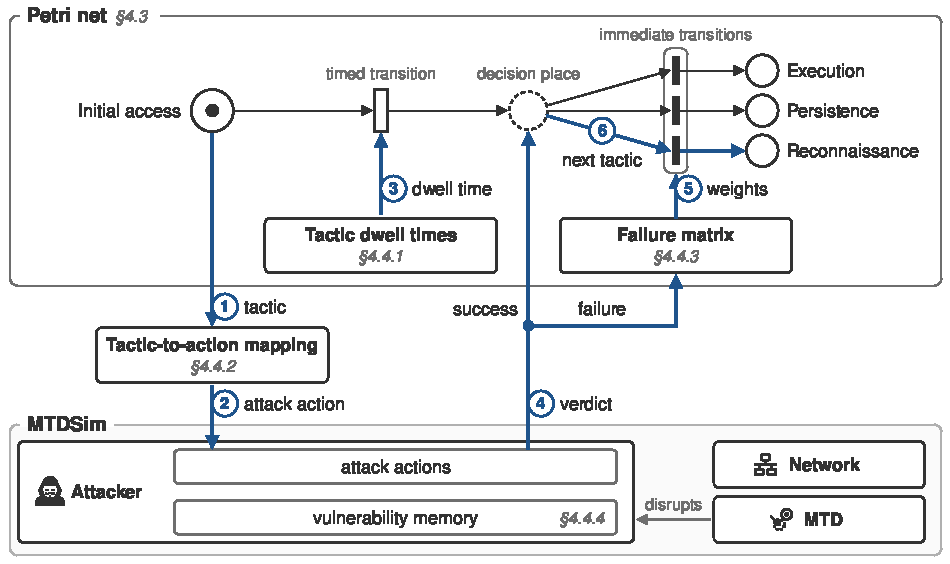
\includegraphics{fig_4-4c_runtime_loop}
  % [CAPTION TIGHTENED 2026-10-04, preamble redraft (Marc: the details flow
  %  into the prose; the quoted step of Figure 4.1 is the section's own
  %  title). DRAFT STATE.]
  \caption[The Petri net integrated with MTDSim]{The Petri net integrated
  with MTDSim, drawn at initial access in $c_1$ with three of its eight
  successors. Blue traces one iteration of the loop, numbered by step.}
  \label{fig:runtime-loop}
% [CH4 SCRUTINY 2026-10-02, F5: regenerated --- "Defender" -> "MTD" (Figure
%  2.1's module), the vulnerability memory drawn in the attacker box in the
%  accent (OWED 2026-09-28, closed); the six steps moved to 4.4.1's prose, so
%  the caption says how to read the bands. DRAFT STATE --- ratify on read.]
\end{figure}

One iteration of the loop runs in six steps, numbered as in
Figure~\ref{fig:runtime-loop}:
\begin{enumerate}[nosep, leftmargin=*]
  \item the token's tactic leaves the Petri net;
  \item the tactic-to-action mapping turns the tactic into one of MTDSim's
  attack actions;
  % [2026-10-05, with Section 4.4.2 round 9 (Marc: "use the specific term on
  %  those two"): "drawn from an exponential" -> "an exponential delay of mean
  %  duration", and the attack action's "cost" -> "time", the terms Sections
  %  2.2.3 and 4.4.2 use. DRAFT STATE.]
  \item the tactic duration, the delay of the tactic's timed transition, is an
  exponential delay of mean duration $\mu_p$, and the attack action runs for
  the tactic duration in place of its own time in MTDSim;
  \item the attack action's verdict, success or failure, returns from MTDSim;
  \item after a failure, the failure matrix reweights the immediate
  transitions (Equation~\ref{eq:routing}); after a success, they keep their
  base weights;
  \item the token fires one immediate transition to the next tactic, and the
  loop repeats.
\end{enumerate}
% [ROUND 3, 2026-10-04 (Marc: "the attack action takes its tactic's drawn time and
%  nothing further does the same as the first part"; "why drawn duration, why not
%  tactic duration as in the diagram"): the replace-not-add rule is one clause of
%  step 3. DRAFT STATE.]
An attack action fails if its preconditions were missing (for example, an exploit of a
vulnerability not yet scanned for), or if an MTD deployment disrupts it
(Section~\ref{subsec:attacker-model}).

% [ROUND 3, 2026-10-04 (Marc: "I still don't think the structure is right";
%  "declared ... who marked their declaration as such"; the four bases "vague";
%  Table C.1 "nuance the reader doesn't need" here). The preamble is three jobs:
%  why (P1), the loop (Figure 4.5 and its steps), what the attack flows do not
%  give (this paragraph). Moved out: the comparison design ("a difference between
%  the two attackers' runs is ... the attacker") to a parked comment at chapter
%  5's setup (out of chapter: Marc to rule); the two declared changes (step 3 and
%  4.4.4 say them); the ceiling to 4.4.2, beside the attack actions' gaps (the
%  chapter 6 pointer follows); the four bases and the three untested values to
%  Appendix C's opener, beside Table C.1 (each subsection states its own basis).
%  Prior text in git 0cbbfa48. DRAFT STATE.]
% [ROUND 4, 2026-10-04 (Marc: "the first sentence is not the important one";
%  "they", "inputs", "the loop reads" vague; "why don't we just use the
%  terminology of the sections"; the source sentence "loses its track"; the
%  memory described too trivially): the three inputs named by their subsection
%  terms as the subject; the sources one clause; the memory said as it works.]
% [ROUND 6, 2026-10-04 (Marc: lead with what the attack flows cannot supply,
%  the paragraph's subject; "their values, whose values?"; the test clause "a
%  given"; the memory "an add-on", subject first): the gap first; "we declare
%  each" names who; the test clause cut; the memory the subject of its sentence.
%  DRAFT STATE.]
% [2026-10-05: the list in the loop's order, as the subsections now run.]
The attack flows cannot supply three inputs of the loop: the
tactic-to-action mapping (Section~\ref{subsec:tactic-verb-mapping}), the
tactic durations (Section~\ref{subsec:dwell-times}) and the failure matrix
(Section~\ref{subsec:failure-matrix}). We declare each, from MTDSim's
constants where they exist and otherwise from the literature or our
judgement. The vulnerability memory (Section~\ref{subsec:vulnerability-memory})
extends MTDSim's exploit attack action: each earlier success on a
vulnerability raises the attacker's odds of exploiting it again.

% [HISTORY: the ruling comments of the 4.4 preamble's paragraphs before the
%  2026-10-04 redraft, kept for the trail; the prose they annotate is in git
%  3ce6e0b5.]
% [CONNECTIVE-PROSE PASS 2026-09-26, P8 4.4 preamble] Connective part only
%  (P8, narrowed: the 2026-09-25 'four bases' paragraph below is ruled and
%  untouched). 'which supplies what the nets cannot' repeated the 4.3
%  bridge; the source-code simile cut; the subsections given roles. The
%  recap paragraph below is removed by the next edit. SESSION-GENERATED on
%  Marc's 2026-09-26 go-ahead (docs/workflows/connective_prose.md; audit
%  docs/implementation/connective_prose_audit.md); prior text in git.
%  RATIFIED 2026-09-26 (Marc: 'I accept all this').
% [ROUND 3 of 4.3, 2026-10-04: "join" retired (Marc); this opener otherwise
%  as ratified 2026-09-26.]
% [CH4 SCRUTINY 2026-10-02, ledger R1--R9, X2, X9, F5, applied on Marc's
%  accept-all: "duration" / "all the tactic timing" -> dwell time (registry
%  row 54, over the 2026-08-20 wording); the loop's six steps moved from
%  Figure 4.5's caption into the prose (F5, re-opens the 2026-09-08 cut); the
%  run-end clause cut (X2: 4.5 states the rule the code runs); the verdict
%  re-declaration and ch2 re-tellings cut (R3, R6); the dwell-only cost named
%  (X9: the model pays the confusion penalty there, movement/attacker.py
%  _pay_interrupt_cost); "sink" -> dead end (R5); Jalowski's ask is ch3's
%  (R7); the extensibility clause to 7.2 (R8). Prior text in git (3f6b4f8c).
%  DRAFT STATE --- ratify on read.]
  % [2026-10-04: steps 2 and 3 swapped to the code's order (movement/attacker.py
  %  _walk: controller.phase_for(place), then timing.draw(place), then the
  %  attack action runs for the drawn time) and to Figure 4.5's lanes.]
% PLACEHOLDER 2026-09-24 (as above; results context §8g-5 content point 1: the
% explicit and the emergent parts of a disruption). Verified: the penalty and the
% lost host are charged by the one call both attackers share
% (attack_operation.py apply_mtd_interrupt_cost); after a host-layer rewrite the
% model's verbs on the lost host return PRECONDITION_UNMET until an enumerate or
% scan host succeeds; the verdict-blind control tracks the model within 0.025.
% [2026-09-25, Marc: 'placeholders comment out': the owed disruption paragraph,
%  commented until dictated; uncomment or replace with the paragraph.]
% \noindent\emph{[Placeholder --- what a disruption does to the APT attacker model,
% explicit and emergent, owed for Section~\ref{subsec:aio-disruption}. Explicit: the
% action in flight fails, the confusion penalty is charged, and a host-layer rewrite
% takes the host the attacker is on --- the same for both attackers, so the
% environment's price is identical. Emergent: the token is not moved; the next
% actions that need the lost host fail their preconditions until the attacker finds
% one again, and the failure matrix routes on those failures. The baseline attacker
% instead restarts its script in a phase set by the layer
% (Section~\ref{subsec:attacker-model}).]}
% [2026-09-20: P2 of the §5.2 split-stream scrutiny (setup handoff §AL1 1b, §AM),
%  session-drafted, accepted by Marc in chat; PLACEMENT IS HIS. Chapter 4 never
%  said the movement attacker takes an objective of Table 2.5, whose caption
%  scopes both to the baseline attacker; §5.2 and Table 5.3 rest on it. Facts:
%  src/mtdsim/l3_simulation/movement/targeting.py (Brown's host-priority rule),
%  attack_operation.py:749-757 (the run ends on a target). Ratify on read.]
% [2026-09-08: ", and produced the join through the controller layer"
%  deleted (the preamble says it); "the firing time of tau_p" bound; the
%  figure pointer folded in from the cut loop paragraph. The "supplies all
%  the tactic timing" clause is the RESOLVED 2026-08-20 wording, untouched.
%  The second sentence is MOVED IN VERBATIM from the tab:dwell-catalogue
%  caption (session-drafted 2026-08-20, landed) --- the replaces-not-adds
%  rule is the clock, so it lives here, not in a caption.]
% [CUT 2026-09-08, both streams: "The loop runs as follows: ..." (75 words)
%  --- fig:runtime-loop's numbered joins and §4.3's routing sentence carry
%  it; "This is verdict-conditioned re-weighting ... encodes direction" moved
%  to the failure-matrix unit; the two sentences restating Eq. 4.4 cut.]
% [2026-09-13: A11 sentences landed on Marc's ratification of the fourteen-item
%  proposal (chat, this date); source register: handoff 2026-09-08_ch4_s43_gspn_formalism.md
%  §7.2. Ratify-on-read.]
% [RESOLVED 2026-08-20 on Marc's wording: the unit's opening claims "all the
%  tactic timing", so the penalty exception no longer contradicts it.]
% [2026-09-08: "Another characteristic is that" and "inherently tied to the
%  simulator; it is" deleted (doubled clauses); "in the Petri net" deleted
%  after "sinks".]
% [RULED, do not re-flag] routing-ablatability must-carry CUT from this unit;
%   guarantee stays repo-side (attacker_state_seam.md); ch6 cites it there.
% [MUST-CARRY: the mapping as a chosen input, the standing caveat bounding
%  every claim in the results chapter (ch5 cites it). Moved 2026-09-08 to
%  close the mechanics unit; ", and that would produce a more useful attacker
%  model" and "We did not have the time to do this." deleted; "Future work
%  can look into changing the underlying action layer, but this has been
%  scoped out for this thesis" cut (the preamble's "scoped it down" and this
%  sentence carry it; ch7 has the future work).]
% [2026-09-26 connective-prose pass: the preamble's "scoped it down" is
%  removed (P8b); this sentence and the ch4 opener now carry the scope.]
% [STRUCTURE 2026-10-04 (Marc: the runtime loop and the preamble are one
%  thing; Figure 4.5 is the headline; each subsection is one declared part
%  of the model, what it is, where its value comes from, what tests it).
%  Roadmap moved here from the opener; "runtime loop" -> "loop" (no
%  subsection by that name now). PURE MOVE otherwise; DRAFT STATE.]
% [CH4 SCRUTINY 2026-10-02, ledger I1--I3, C4, X6, applied on Marc's
%  accept-all: the OWED 2026-09-28 memory clause landed (I1) and the factor of
%  three joins the judgement list (I2); "Appendix B gives the reason for each"
%  was false for sigma and one flow per group (X6: no row in Appendix B), so
%  the pointer is split by where each reason lives; the ablation and
%  sensitivity previews cut (I3: each subsection points at its own test, and
%  5.4 opens on the list); ten Broeke moved to 4.4.2. Prior text in git
%  (3f6b4f8c). DRAFT STATE --- ratify on read.]
% [OWED 2026-09-28: with Section~\ref{subsec:vulnerability-memory} this
%  sentence needs the memory: "three inputs the join carries" plus "and
%  Section~\ref{subsec:vulnerability-memory} the attacker's memory of the
%  vulnerabilities it has exploited" (the memory sits in the exploit action, not
%  in the join's routing); and the bases list below gains $\lambda$ among the
%  values that are our judgement. Marc's wording.]
% [CUT 2026-09-08, both streams] the mutation example ("Suppose, for
%  example, the attacker is thwarted ... follow the next tactic. This was not
%  representative ..."): §4.3 carries the argument ("needs them to depend on
%  what happened in the simulator") and the example ("cut short by an MTD
%  mutation, which returns failure"). Reversible from git 9a333c48.
% [E2 SWEEP 2026-09-22: the three layer names DISSOLVED on the supervisor's
%  ruling (not layers; names only on a needs basis) and Marc's (no names).
%  What L0--L3 produce is the profile net; what MTDSim has is the baseline
%  attacker's verbs; what L4 declares is the join --- this section's own
%  heading. DRAFT STATE, ratify on read.]
% [rephrase applied per your ruling: the two "beside MTDSim" sentences folded
%   into one, "beside" carried once.]
% [spine sentence --- Marc's dictation 2026-08-19; moved up 2026-09-08 as
%  the section's contract, bound to the three symbols; "is the join between
%  the Petri nets and our simulator, and it" deleted (the sentence above
%  says the controller is the join), "(the stochastic dwell times)" deleted
%  (the parameter is the mean; the draw is what is stochastic).]
% [CONNECTIVE-PROSE PASS 2026-09-26, P8b 4.4 preamble] Removed: the recap
%  of 4.1-4.3 and chapter 2, 'We scoped it down' (the 4.4.1 ceiling
%  paragraph carries the scope; drop its pointer to 'the preamble's scoped
%  it down'), the either-or design (fifth statement; ch1, Figure 4.1's
%  caption and 4.4.1 keep it), and the spine sentence's colon-list (the
%  4.3 bridge lists the inputs with their symbols one line earlier; the
%  Equation 4.1 pointer for mu_p was wrong anyway). Overturns the
%  2026-08-19 spine sentence on merit. SESSION-GENERATED on Marc's
%  2026-09-26 go-ahead (docs/workflows/connective_prose.md; audit
%  docs/implementation/connective_prose_audit.md); prior text in git.
%  RATIFIED 2026-09-26 (Marc: 'I accept all this').
% [2026-09-25 SUPERVISOR SCREEN, step 1 (Marc: "just push it in for now";
%  conventional terms over descriptive ones). REPLACES "We chose each of them
%  to the best of our judgement after consulting the literature; whether any
%  conclusion of the evaluation depends on where a chosen value sits is the
%  question Appendix~\ref{app:sensitivity} answers." The four bases are Marc's
%  ruling; "one-factor-at-a-time" and "nominal values" are ten Broeke et al.'s
%  terms (docs/sources/methodology/tenbroeke2016_abm_sa.md), which name what
%  Appendix C does. Record: docs/handoffs/2026-09-25_ch4_mark_risk_ledger.md.
%  DRAFT STATE, ratify on read.]

% INSERTION A APPLIED 2026-09-18 --- DRAFT STATE, ratify on read (Marc's
%  green light this date: "swept is wrong, we kind of just chose them ... we
%  chose them to our best of knowledge after consulting the literature").
%  Replaces "; each is swept in the sensitivity analysis (Section 5.1)."
%  Why: "swept" is the wrong verb for the mapping (a comparison against one
%  alternative) and for the nine failure rules (held); and it misreports how
%  the values were arrived at. The clause now names the question §5.1
%  answers. Prior wording and its 2026-09-13 note are in git (32e309bb).
%  Source register: handoff 2026-09-17_ch5_s51_sensitivity_overhaul.md D5
%  insertion A + S5 defect D-4.

% [SUBSECTIONS REDRAFT 2026-10-05 (Marc: each subsection "a collection of
%  sentences", added one ruling at a time; "we did this, here are the numbers";
%  the purpose missing; terms drifting from the preamble). One skeleton for all
%  four: what the input does in the loop (its step of Figure 4.5) and why the
%  attack flows cannot give it; what we declared, and from what, with one worked
%  example; how many values it adds, its limits and its test. Reordered to the
%  loop: the mapping (step 2) before the durations (step 3); Figure 4.5's box
%  numbers and the preamble's list swapped with it. Terms to the preamble's:
%  MTDSim (not "the simulator"), immediate transitions (not out-transitions),
%  attack profile, Petri net. Prior text and every ruling comment of these four
%  subsections: git 1aa0143e. Rulings carried forward are named in each
%  subsection's comment. DRAFT STATE.]
\subsection{Tactic-to-action mapping}
\label{subsec:tactic-verb-mapping}

% [ROUND 4, 2026-10-05 (Marc: "100% on the right track", but the sentences
%  lose clarity: "Figure 4.6 draws it" draws what; the tactic-technique
%  relation unexplained; the colon clauses say the same thing twice; "direct"
%  and "broad" undefined, a false dichotomy; "several tactics can share one"
%  one what, and why; "the technique or the reason" when every row needs a
%  reason; three unmapped reasons in the prose and four pushed to the appendix
%  "seems shifty"). One idea per sentence, subject first, no colon
%  restatements. The tactic and technique as Section 2.x defines them (what an
%  attacker does to achieve a goal; how it does it). Six tactics map by
%  technique (Brute Force under credential access, v19.1); the three that
%  share the exploit say why; the other two by the goal the attack action
%  serves, "we chose" (no claim that no attack action carries out a technique
%  of lateral movement: Exploitation of Remote Services exists). "Direct" and
%  "broad" cut. Every unmapped reason in the prose, one sentence each (Table
%  B.5's). The runtime sentences and the ceiling kept as Marc read them.
%  "Tactic-to-action mapping" emphasised at its definition, as Section 4.3
%  does its terms (the preamble only names it). Round 3 in git dec299d6.
%  DRAFT STATE.]
% [ROUND 5, 2026-10-05 (Marc: on the right track; round 4's short sentences
%  "choppy", losing the flow; "Brute Force ... maps to brute force", the
%  capital lost on the reader; "six tactics map this way" vague). The
%  technique said in words where its name would echo the attack action's
%  ("guessing passwords by brute force", ATT&CK's T1110); all six tactics
%  mapped by technique named, in two sentences, so "six" is not needed
%  (reconnaissance: Active Scanning, discovery: Network Service Discovery, both
%  scanning techniques, v19.1); the two chosen for their goal in one sentence
%  each. Paragraphs two and three as round 4. DRAFT STATE.]
The \emph{tactic-to-action mapping} turns the token's tactic into one of
MTDSim's attack actions at step~2 of Figure~\ref{fig:runtime-loop}.
Figure~\ref{fig:controller-mapping} shows the attack action each of the 15
tactics maps to, if any. We declared each pair from ATT\&CK, in which a
tactic is what an attacker does to achieve a goal and its techniques are how
it does it (Section~\ref{subsec:attack}). A tactic maps to the attack action
that carries out one of its techniques. Credential access, for example,
includes guessing passwords by brute force, which is what MTDSim's brute
force attack action does. Initial access, execution and privilege escalation
each include a technique that exploits a vulnerability, so all three map to
exploit, and reconnaissance and discovery each include a scanning technique,
so they map to scan host and scan port. For the remaining two, lateral
movement and command and control, we chose the attack action that serves the
tactic's goal. Enumerate host moves the attacker to its next host, which is
the goal of lateral movement, and Brown describes scan neighbours as command
and control revealing connected hosts~\citep{brown2023}.
Table~\ref{tab:controller-mapping} gives the reason for each tactic.

% [figure LANDED 2026-08-20. Generated by tools/controller_mapping_figure.py
%   from data/ogasp/controller/mappings/v2_partial.csv, the pinned ATT&CK
%   bundle and lifecycle_consensus.json (stage bands). Round 3, 2026-10-05:
%   the column header "MTDSim attack action" and the key "unmapped" carry what
%   the caption decoded; [tbp], with Figure 4.5. Round 4: "grouped by", the
%   four stages named as Section 3.1.1 names them. Ratify-on-read.]
\begin{figure}[tbp]
  \centering
  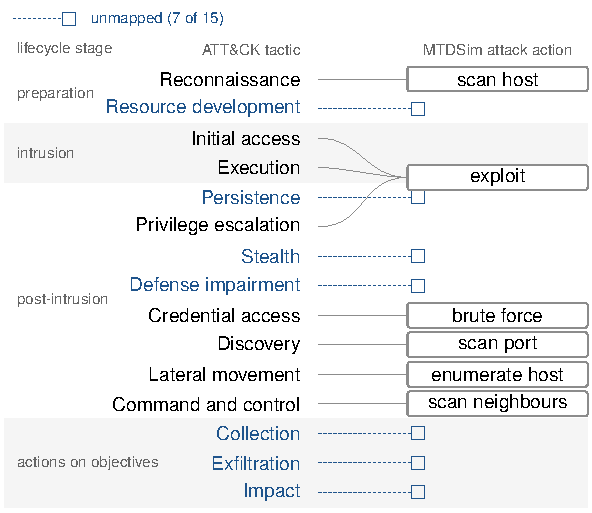
\includegraphics{fig_4-4a_controller_mapping}
  \caption[The tactic-to-action mapping]{The tactic-to-action mapping, with
  the tactics grouped by the four lifecycle stages of
  Section~\ref{subsec:apt}.}
  \label{fig:controller-mapping}
\end{figure}

Seven tactics are unmapped, because no attack action in MTDSim carries them
out. MTDSim's attacker stops at compromising hosts, so collection,
exfiltration and impact have nothing to act on. Nothing in MTDSim watches
the attacker, so stealth has nothing to hide from. The attacker can neither
see nor change the MTD schedule, so defense impairment has nothing to
impair. A compromised host stays compromised, so persistence has no foothold
to keep. Resource development happens off the target's network, which
MTDSim does not model.

An unmapped tactic still takes its duration, but it dispatches no attack
action, so it cannot fail. Its immediate transitions therefore keep their
base weights, as after a success (Section~\ref{sec:petri-formalism}). An MTD
deployment during an unmapped tactic cuts the duration short and costs the
attacker the confusion penalty, but it cannot change which tactic comes
next. The unmapped tactics are the gaps in MTDSim's attack actions, and
those attack actions set the ceiling of this dissertation: the APT attacker
model can only be as good as the attack actions it adopts.

\subsection{Tactic durations}
\label{subsec:dwell-times}

% [ROUND 6, 2026-10-05 (Marc: rounds 4-5 "cycling the same vague and
%  hard-to-follow reasoning" from P4 on, "typically means the structure is
%  wrong"; look for how the field presents judgement values; mean duration
%  never defined; six paragraphs not warranted). Restructured on the field's
%  guidance (docs/implementation/pipeline/ogasp/
%  judgement_parameter_presentation_guidance.md: ODD 2020, TRACE 2014, STRESS
%  2019, Briggs 2012, Saltelli 2019, McQueen 2006): a parameter table carries
%  each value, its source and, for a judgement, the two times it was placed
%  between; the judgement is stated once as an assumption, with one worked
%  example, and not argued further; the robustness test is a separate
%  paragraph in the field's order (what it tests, what moves, the bands and
%  what they measure, the output and criterion fixed before the run, the
%  one-at-a-time limit and the untested comparison with the baseline
%  attacker, the result). P1 defines the mean duration through the
%  exponential delay, so the old closing paragraph folds in; the shape test
%  joins the robustness paragraph. Five paragraphs. Round 5 in git 7c3b9598.
%  DRAFT STATE.]
The \emph{tactic durations} set how long each tactic takes, at
step~3 of Figure~\ref{fig:runtime-loop}. They set the APT attacker model's
pace, and the longer a tactic runs, the more likely an MTD deployment
disrupts it. A tactic's duration is random each time it runs, an
exponential delay, because the timed transitions of a GSPN fire after
exponential delays (Section~\ref{sec:petri-formalism}) and attack behaviour
is stochastic~\citep{holm2014, madan2004, bland2020}. An exponential delay
has one parameter, its mean, so each tactic needs one value, its
\emph{mean duration}~$\mu_p$.

MTDSim cannot supply every mean duration. The Petri net times each tactic,
but MTDSim times only its attack actions, and seven tactics are unmapped
(Section~\ref{subsec:tactic-verb-mapping}). MTDSim does not carry an
unmapped tactic out, but the tactic still takes the attacker time. Each
tactic therefore has a mean duration of its own, and the attack action it
maps to runs for the tactic's duration in place of the attack action's time.
Table~\ref{tab:dwell-catalogue} gives each mean duration and its source:
MTDSim for six tactics, and our judgement for the other nine.

% GENERATED by tools/dwell_catalogue_tables.py from
%   data/ogasp/tactic_durations.json (v0-uncalibrated); tactic axis and
%   display names from the pinned ATT&CK bundle (v19.1).
% Do not hand-edit; regenerate. Requires booktabs (already in the preamble).

\begin{table}[htbp]
\centering
\caption[The tactic durations]{The mean duration of each tactic, with what it was set from. Appendix~\ref{app:dwell-derivation} gives each tactic's reason.}
\label{tab:dwell-catalogue}
\tablestyle
\begin{tabular}{@{}P{0.29\textwidth} P{0.21\textwidth} P{0.21\textwidth} r@{}}
\toprule
Tactics & What they do & Set from & Mean duration $\mu_p$ (s) \\
\midrule
Initial access, privilege escalation, credential access, lateral movement & A brief act on one host & MTDSim's median exploit cost & 4.5 \\
Reconnaissance, discovery & Survey hosts & MTDSim's three scans ($5 + 25 + 5$\,s) & 35.0 \\
Persistence, stealth, command and control & Kept up quietly over time & Declared & 45.0 \\
Execution, defense impairment & Short acts among the quiet tactics & Declared & 22.5 \\
Collection, exfiltration, impact & Move or destroy data & Declared & 36.0 \\
Resource development & Off the network, before the attack & Declared & 0.0 \\
\bottomrule
\end{tabular}
\end{table}


% [ROUND 10, 2026-10-05 (Marc: the nine judgement values never clear in any
%  version, "inherently arbitrary"; "I'm not sold on that argument"; P3 lost at
%  credential access; P4 dense; P5's NCR numbers read as results; honesty and
%  transparency lost. Ruled: write the assumptions cleanly, declare the numbers
%  as their extension, our judgement; one pointer plus a one-clause verdict,
%  as 4.4.3 and 4.4.4). P1, P2 and Table 4.2 unchanged. P3: the credential
%  access example to Appendix B.4 (its row gives the reason); the rule it
%  illustrated kept as one clause ("even where the tactic maps to another":
%  four of the six map elsewhere, so without it "takes that attack action's
%  time" is false). P4: each group's reason said as the judgement it is, the
%  45 s grounded in ATT&CK's tactic descriptions (persistence "maintain their
%  foothold", stealth "hide and conceal", command and control "communicate
%  with systems under their control", enterprise-attack 19.1); "placed between
%  two times" CUT (it read as a derivation of a judgement); "CTI vendor
%  reports" -> "threat reports" (the defined term). P5: the caveat ("model
%  parameters for this simulator, not real-world values", Marc's dictation,
%  as 4.4.3) answers "why 45 s when persistence lasts months"; "nearly every"
%  -> "most" (an exponential of mean 200 s outlasts a 200 s interval in about
%  63 per cent of runs); the test as one clause, true of Table C.1a (4.5 s is
%  inert, so "depends most on", not "depends on them"); "run after the values
%  were fixed" is Appendix C.1's own statement. Half of 45 s kept (Appendix
%  C.1 and C.2 rely on it). Cold-read and audited (scratchpad reviews).
%  DRAFT STATE.]
Six tactics do the same kind of work as one of MTDSim's attack actions, so
each takes that attack action's time, even where the tactic maps to another
(Section~\ref{subsec:attacker-model}). Initial access, privilege escalation,
credential access and lateral movement each act briefly on one host, as the
exploit attack action does, so each takes the mean time of the exploit attack
action, 4.5~s. Reconnaissance and discovery survey a network, as MTDSim's
scans for hosts, ports and neighbours do together, so each takes the total
time of the three scans, 35~s.

No source times the other nine tactics, since threat reports time whole
intrusions. We set their mean durations by judgement, from what each tactic
does in an attack, as other models that time attack steps do where data are
missing~\citep{mcqueen2006, bland2020, mendonca2023}.
Chapter~\ref{ch:experiments} compares the APT attacker model with the baseline
attacker under the same MTD deployments, so we kept the nine on the scale of
the baseline attacker's attack actions (Section~\ref{subsec:attacker-model}).
We also kept each under the 200~s default deployment interval
(Section~\ref{subsec:defence-mechanisms}), or a deployment would disrupt most
runs of the tactic.

Persistence, stealth
and command and control keep a foothold, stay hidden and stay in contact
throughout an attack~\citep{mitre2026attackkb}, so we set them longest, at
45~s. Collection, exfiltration and impact move or destroy data, which we
judged to take a little longer than surveying a network, so we set them at
36~s. Execution and defense impairment are single acts that the attacker
paces to stay hidden, so we set them at 22.5~s, half the 45~s and longer than
an exploit. Resource development happens before the attack reaches the
target's network, so it takes no time.
% ROUND 11, 2026-10-05 (Marc: as in 4.4.3, the last paragraph repeats the
% judgement and could be integrated into the existing paragraphs). The
% judgement sentence is cut (P2 and P4 say it; P1's scale sentence carries
% "not real-world values"); the 200 s bound joins P1, where the scale is set
% and the disruption risk stated, since it holds for all fifteen; the test
% closes P4, as 4.4.3 and 4.4.4 close on theirs. DRAFT STATE --- ratify on read.
% ROUND 12, 2026-10-05 (Marc: P1 set the scale before P2 said where the values
% come from; the C.1 sentence vague, "moves", "share", "across a band", "one at
% a time"; "so what"; the 45 s matters through the mapping, a model fact, not
% a fact about the tactics). Accepted as proposed: the scale and the 200 s
% bound move from P1 to P4, the judgement they constrain; the groups become P5,
% closing on the test in plain words: why, what, the finding, the likely
% reason (the test moved the three tactics together, hence "most likely"),
% and what it means for chapter 5. Checked: per doubling the 45 s moves NCR
% about four times as much as any other value, so "only" is fair across the
% unequal bands. DRAFT STATE --- ratify on read.
Because these values are our judgement,
Appendix~\ref{app:dwell-robustness} tests whether NCR
(Section~\ref{sec:evaluation-metrics}) depends on them: after the values were
fixed, it halved and doubled each one in turn. Only the 45~s changes NCR much,
most likely through command and control, one of the three tactics it times.
Command and control is the only tactic that maps to scan neighbours, the
attack action that finds the hosts next to those the attacker has compromised
(Section~\ref{subsec:tactic-verb-mapping}). The slower the attacker finds new
hosts, the fewer it reaches before the run ends, so Chapter~\ref{ch:experiments}'s
NCR rests most on this one value.

\subsection{Failure matrix}
\label{subsec:failure-matrix}

% [REDRAFT 2026-10-05. Added: the job (step 5); the scale of what Appendix B.6
%  holds (Marc: "is it disingenuous to hide them"): twelve declared values set
%  all 210 factors, verified (v4_failure_only: 15 sources x 14 destinations;
%  nine rules A-I, gamma, delta, z), parallel to 4.4.2's four-not-15; the
%  completeness assumption said as it bears on F (F only reweights the
%  immediate transitions the attack flows draw). CUT: survivorship told twice
%  more (Section 4.3 owns it, "an attack flow draws only the steps its attacker
%  completed"; 4.4.3 points there once); "fails upwards" folded into the test
%  sentence (4.3 carries "would carry on as though it had succeeded");
%  "A rule of forward and backward alone does not fit" (argued against an
%  alternative the reader never saw; the 58-71 figure now says what it shows);
%  "Eight of the 15 tactics ..."; the caveat (said once, in 4.4.2; "every value
%  is our judgement" and "No value was fitted" carry it here); "not two" (a
%  flourish). The dead end stays beside the stall: the retrace depends on the
%  edge the token travelled, which a GSPN marking does not hold, so Section
%  4.3's construction cannot state it (the critique's move to 4.3 withdrawn).
%  Kept, ruled: the principle and the foothold (F-ledger 2026-10-02), the
%  ATT&CK-order sentence, the worked example, the disruption sentence (A5), the
%  stall (A10, verified controller/outcome.py). Test pointer to Appendix C.3
%  (decay-robustness: gamma, delta, z). DRAFT STATE.]
% [ROUND 2, 2026-10-05 (Marc: the section "basically unrecognisable" from his
%  dictation, whose words he chose with care; "failure matrix" not defined at
%  first use in the subsection; "one principle" then "twelve values"; Figure
%  4.4(b) unexplained, "why are we jumping sections"; the worked example a
%  whole paragraph; what is here and what is in the appendix; loses structure
%  midway). Structure of 4.4.1, which reads clearly: the term defined at its
%  step of the loop, then why, then how its values were set with one example,
%  then its limits and its test. Marc's dictation (commit 3950c543, 2026-08-20)
%  restored where it still holds: "We employed a failure matrix because this
%  is the blind spot of the CTI"; the reports are incidents "worth writing
%  about"; "we didn't reverse-engineer any of these values"; the two
%  components, rules and distance; "it makes no sense for an attacker to go
%  from recon directly to impact"; "a concession of the thinness of the
%  corpus"; the must-carry caveat (cut in round 1 as said in 4.4.2, which no
%  longer says it). The survivorship reason now lives here, where Section 4.3
%  points for it (4.3 and 4.4.3 each pointed to the other). "One principle"
%  CUT: verified against v4_failure_only, it held for post-intrusion operations
%  only (same-stage share 0.65 -> 0.76 after a failure); at actions on
%  objectives a move back one stage has 0.9 (rule F) against 0.7 within, and
%  the shares do not move (0.85 back, before and after). The prose now states
%  the foothold split and the factors it gives, all true of Table B.6a. The
%  stall CUT: verified, no place of any net loses every exit at the declared
%  values or anywhere in the tested bands (no net carries a three-stage move,
%  so the floor never binds), so the sentence described a case that never
%  occurs (overturns ruling A10 on merit; Marc to confirm). Kept, ruled: the
%  foothold, the ATT&CK-order sentence, the worked example (now two
%  sentences), the one-verdict limit (A5) in the preamble's words, the dead
%  end, the ablation and Appendix C.3 pointers. Numbers re-run 2026-10-05:
%  c1 initial access, reconnaissance 0.062 -> 0.750, foothold moves to about a
%  quarter (factor 0.02 against 0.9); 58-71 per cent from
%  tools/gspn_gadget_figure.py stage_shares. DRAFT STATE.]
The \emph{failure matrix} reweights the immediate transitions after an attack
action fails, at step~5 of Figure~\ref{fig:runtime-loop}. It holds one factor
between zero and one for each pair of tactics, the tactic whose attack action
failed and a tactic that can come next, and Equation~\ref{eq:routing}
multiplies each base weight by its factor. We employed a failure matrix
because failure is the blind spot of the CTI. The threat reports behind the
attack flows describe incidents that succeeded and were worth writing about,
so an attack flow draws only the steps its attacker completed. The base
weights therefore say where an attacker goes after a success, and nothing
about where it goes after a failure.

% [ROUND 3, 2026-10-05 (Marc on round 2: P1 good; the bare factors "carry no
%  meaning", only relative ones do; "nine rules", cite the appendix; the
%  distance factor, "a stage beyond the next", the 0.25 and the floor vague;
%  P4 "alike" vague; think of the examiner's questions: where do the values
%  come from, did you set 210 numbers by hand, how do you know they are
%  right). P1 unchanged. The rest answers the examiner in order: where the
%  values come from and how twelve values set 210 factors (a script, first
%  matching rule, verified: rules.py _failure_rule; outcome_rules.json
%  "values are RULE-GENERATED"); why a factor only means something against
%  the others of its tactic (Equation 4.5 renormalises); what the rules do,
%  as the code orders them (back 0.9 over same stage 0.7 over forward 0.35,
%  then the two foothold gates and the dampers, said as stages), with the
%  example carrying the motivation; the distance factor tied to the lifecycle
%  stages of Section 3.1.1, its floor left to Appendix B.6 (no net has a
%  three-stage move, so it never acts); the limit said as a consequence; the
%  dead end as the other routing limit; how we know: no data, so model
%  parameters, and the ablation's finding in Marc's words (2026-09-28: it
%  "changes where the attacker goes but doesn't change what it achieves").
%  CUT: the 58-71 per cent sentence (base weights, not factors; record in
%  tools/gspn_gadget_figure.py stage_shares). DRAFT STATE.]
% [ROUND 4, 2026-10-05 (Marc: never understood the nine rules, presented
%  "like a black box"; "why don't you just use 15 rules"; the values
%  "inherently arbitrary", and the honesty and transparency lost; how do 210
%  values beat random noise. Ruled: the rules are assumptions about attacker
%  behaviour; write the assumptions cleanly, grounded where they can be, and
%  declare the numbers as their extension, our judgement; a pointer plus a
%  one-clause verdict). P1 unchanged (approved). P2 the three assumptions,
%  each with its ground: the foothold (Section 2.x lifecycle stages) and
%  Hutchins' campaign that tried again the next day with a new recipient
%  list after its attempt was "detected and mitigated" (his words; "blocked"
%  is the MTD term here); the second openly our judgement; the third the
%  lifecycle models. Said as likelihoods, true of the factors: in the rules a
%  same-stage move after a failure with a foothold gets 0.7 and every other
%  move open to a tactic that can fail gets at most 0.35 (the 0.9 "back" rule
%  never fires for a mapped tactic with a foothold). P3: the rules as the
%  assumptions written down, nine because the assumptions tell nine kinds of
%  move apart; the distance factor named (Appendix B.6 relies on it); the
%  renormalisation clause restored (without it "rises from 0.062 to 0.750"
%  contradicts a factor at most one); the c1 example kept with its
%  motivation (re-verified). P4 what it gives (adaptivity, property 4, as
%  Section 5.4 and Table 7.1 say) and its limits: verdict only; it reweights
%  only the next tactics the attack flows give (c2: no move from initial
%  access back to preparation, as Section 5.4.2 reports); the dead end (all
%  four nets have one; Marc's "concession to the thinness of the corpus").
%  P5 judgement, caveat, both tests. CUT: the rule-by-rule values, "first
%  matching rule", the distance factor's 0.25. "from the corpus" dropped from
%  "did not reverse-engineer": the rules were checked against routing on the
%  nets in 2026-07 (outcome_rules.json scrutiny). Cold-read and audited.
%  DRAFT STATE.]
We set the failure matrix from three assumptions about what an attacker does
after a failure. First, an attacker without a foothold
(Section~\ref{subsec:apt}) is unlikely to go on to a tactic that needs one, so
after a failed initial access it is likely to go back to preparation to try
again. Hutchins et al.\ describe an APT campaign that tried again the next
day, with new recipients, after its intrusion attempt was detected and
mitigated~\citep{hutchins2011}. Second, an attacker that fails after it has a
foothold keeps the foothold, so we judged it more likely to try another
tactic of the same lifecycle stage than to move to another stage. Third, an
attacker seldom skips a lifecycle stage, as in the lifecycle models of
Section~\ref{subsec:apt}, which run their stages in sequence.

We wrote the assumptions as rules instead of setting the 210 factors one by
one. Nine rules give one value to each kind of move the assumptions tell
apart, such as a move to another tactic of the same lifecycle stage after a
failure with a foothold. The third assumption is also written as a distance
factor, which scales a move down by each lifecycle stage it skips. The rules
and the distance factor set all 210 factors (Appendix~\ref{app:weight-sets}),
and their values are our judgement. Equation~\ref{eq:routing} rescales
the weights out of a tactic to sum to one, so a factor counts only against
the other factors of the same tactic. After a failed initial access in
$c_1$, for example, the weight on reconnaissance rises from 0.062 to 0.750
(Figure~\ref{fig:gspn-gadget}(b)), so the attacker most likely goes back to
reconnaissance to try again. Without the failure matrix, it would most likely
carry on into the network as though it had broken in.

The failure matrix gives the APT attacker model adaptivity, property~4 of
Table~\ref{tab:attacker-properties}: it chooses its next tactic in response
to a failure, including one caused by an MTD disruption. It reads only the
attack action's verdict, so it treats a disruption as any other failure. The
failure matrix can reweight only the next tactics the attack flows give. In
$c_2$, no move leads from initial access back to preparation, so a failed
initial access still goes on into the network. Where the corpus gave a
tactic no next tactic, a dead end, there is nothing to reweight, and the
token retraces the edge it travelled, a concession to the thinness of the
corpus. Section~\ref{subsec:ablation-failure-matrix} sets
every factor to one and finds that the failure matrix changes where the
attacker goes after a failure, but not what it achieves.

% ROUND 5, 2026-10-05 (Marc: the last paragraph says again what is said
% everywhere else; "I thought the distance factor was one value ... judgement
% calls within a judgement call ... can we abstract it away"; the c1 example
% did not visibly link to the sentence after it). Done: the distance factor is
% the third assumption written down, its three values (two rates, a floor) left
% to Appendix B.6, whose table caption still points to Appendix C.3; "twelve
% values", "model parameters ... not real-world values" (4.4.2 says it) and "did
% not reverse-engineer" cut; one sentence declares the values judgement; the
% c1 example says what the rise does (base weights from initial access in c1
% put 0.938 on tactics past the foothold, checked 2026-10-05). Hutchins kept on
% merit: the ground of assumption 1, not literature-review content (Marc asked
% for grounded assumptions). Then (Marc, same read: the last paragraph
% "could just be integrated better into the existing" ones): the judgement
% clause joins P3 where the values come in, the test closes P4, so the
% subsection still ends on its test as 4.4.4 does. DRAFT STATE.

\subsection{Vulnerability memory}
\label{subsec:vulnerability-memory}

% [REDRAFT 2026-10-05. Reordered: what the memory does, why (the recurrence
%  across hosts), its lineage, property 7 and its limit, the hypothesis and its
%  test. The lineage now says why the memory raises the chance of success
%  rather than halving the time, as Zhang does: the tactic duration replaces
%  the exploitation time (step 3), so a halved time would change nothing; this
%  is what "tactic durations still come from Section 4.4.1" was carrying. The
%  model-wide scheme-aware paragraph folded in as the limit of property 7,
%  with the OWED 2026-09-28 clause landed ("learns nothing about the defence",
%  Marc's wording; verified 2026-09-13: movement/learning.py never reads the
%  schedule). Kept, ruled: "triples" (adversary.py:290-305), the CVSS odds,
%  property 7 in part (B0, 2026-09-29), the diversity-pool hypothesis and its
%  test (handoff Part A). DRAFT STATE.]
% [ROUND 1, 2026-10-05 (Marc: drafted in piecemeal, "not in the frame" of
%  4.4, which extends the model; "the motivation isn't really there ... why
%  did we have to add it"; important point and subject first; what nuance the
%  examiner does not need). Three paragraphs, one examiner question each: what
%  it is and why it had to be added (P1), how it works and where its value
%  comes from (P2), what it gives and what we expect of it (P3). The why is in
%  the frame of 4.4: the baseline attacker's one form of learning, the halved
%  exploit time (Section 2.2.3; Section 3.3.2 scores the lineage's learning
%  partial for it), cannot reach the APT attacker model, because step 3
%  replaces the exploit's time with the tactic duration. Corrected: "Zhang et
%  al." (zhang2023 is single-author, as ch3 was corrected 2026-09-29); "CVSS
%  complexity" -> "attack complexity" (Section 2.2.1's term); "draw" (retired).
%  Added: the baseline attacker runs without the memory (run_corpus.py: the
%  rate is set for the movement arm only); the memory lasts the run and no
%  deployment erases it (adversary.py: the counts are reset nowhere).
%  Overturned on merit: the property 8 sentences (each run starts from M_0;
%  "not scheme-aware") leave this section, as they describe the whole model,
%  not the memory; the chapter opener, Section 6.5 and Section 7.2 already say
%  it. "Learns the network" -> Section 3.3.2's own words, "learns about
%  vulnerabilities, not about the MTD deployments it observes". Kept, ruled:
%  "triples the odds", the factor as our judgement, property 7 in part (B0),
%  the diversity-pool hypothesis and its test. DRAFT STATE.]
% [ROUND 2, 2026-10-05 (Marc: P1 "very strong", but S3 clunky ("an exploit
%  of a vulnerability it has exploited") and the last sentence four clauses;
%  "the baseline attacker runs without the memory" wrong, it has its own, the
%  halved exploit time ("the original vulnerability memory"); "the halving"
%  vague; "erases" not the word; two pointers to Section 5.4.3; P2 and P3 split
%  for no reason, learning belongs with the why). Two paragraphs: why (P1,
%  property 7 now closes it), how and what we expect (P2, the recurrence leads
%  into the hypothesis). One pointer to the ablation. The baseline's halved
%  time is named as a memory; the memory "updates an existing feature and
%  beefs it up" (Marc). "Like the halving" cut. DRAFT STATE.]
The \emph{vulnerability memory} extends MTDSim's exploit attack action so that
the APT attacker model is more likely to exploit a vulnerability it has
exploited before. An attacker that remembers which exploits succeeded can
reuse them, and so succeeds more often as its attack goes on. The baseline
attacker already remembers the vulnerabilities it has exploited: exploiting
one again takes it half the time (Section~\ref{subsec:attacker-model}). In the
APT attacker model, the tactic duration replaces the exploit's time (step~3
of Figure~\ref{fig:runtime-loop}), so the baseline attacker's memory saves it
no time. The vulnerability memory acts on the chance of success instead. It
gives the APT attacker model learning, property~7 of
Table~\ref{tab:attacker-properties}, in part: it learns about
vulnerabilities, not about the MTD deployments it observes.

Each earlier success on a vulnerability, on any host, triples the attacker's
odds of exploiting it again (the odds its attack complexity sets,
Section~\ref{subsec:network-model}). The factor of three is our judgement.
The memory lasts the whole run, through every MTD deployment. Hosts that run
the same service carry the same vulnerabilities, so the attacker meets the
same vulnerability on more than one host. We therefore expect the memory to
matter more when the \emph{diversity pool}, the services each operating
system can run, is small, because hosts then run the same services more
often. % [2026-10-05, with 4.4.2 round 10 and 4.4.3 round 4 (Marc: the three
%  subsections handle the test the same way, a pointer plus a one-clause
%  verdict). Verdict from Section 5.4.3: exploit success 0.70 -> 0.73 at 20
%  services, 0.69 -> 0.91 at one; NCR d below 0.2 at every pool. DRAFT STATE.]
Section~\ref{subsec:ablation-vulnerability-memory} tests this expectation,
and finds that the memory raises the share of exploits that succeed, most
with a small diversity pool, but leaves what the attacker achieves unchanged.

\section{Evaluation metrics}
\label{sec:evaluation-metrics}

% ROUND 4, 2026-09-29 (Marc's second read; voice.md §(0), "say more with
% less"). Applied rulings: attack confidentiality on Snort's default scan rule
% (E); the compromise rate after an MTD deployment and time lost per MTD
% deployment on the half interval (F, folding in A); no MTD for no defence
% (G1); APV replaced by distinct attack paths, the count Marc asked for; the
% targeted scenario stated; the cell defined in 4.5.4; statistics signposted.
% OPEN: ruling H (MTTC at the target, and the general scenario's 80 % stop
% inside targeted runs) in handoff 2026-09-29_ch4_consolidation.md; the MTTC
% and run-end sentences below state the corpus as it stands. Chapter 5 is
% stale against this section by Marc's ruling (ch4 first); the owed list is
% in the same handoff. Rounds 2-3 in git. DRAFT STATE --- ratify on read.
% ROUND 7, 2026-10-05 (Marc: section 4.5 "was kind of like an add on", not in
% the frame of the method; "why do we need this"; the opener "Chapter 5 answers
% SQ3 with the metric tables" says where, not why). Accepted as proposed: P1 is
% the frame (SQ3 needs three kinds of metric, named once as the subsection
% titles; the field's are adopted; they depend on the attacker but record only
% what it achieves, so behaviour metrics are added; whole-run effectiveness
% metrics cannot show the response to a deployment, so two per-deployment ones
% are added). "How well MTD stops it" is Section 3.2.2's definition verbatim.
% P2 is the old scope sentences, unchanged, the combination first.
% DRAFT STATE --- ratify on read.
% ROUND 8, 2026-10-05 (Marc: P1 vague and rhetorical --- "takes metrics of
% three kinds", the second-rate gloss of each kind, "their metrics", "can be
% read as", the "only if ... acts as an APT attacker does" riddle, "read a whole
% run"; P2's "combination" and targeting rule unclear; "why two paragraphs";
% the motivation lost). One paragraph: SQ3 in its own words; the field's attack
% outcome and MTD effectiveness metrics adopted; no MTD metric measures how an
% attacker behaves, so the added ones, named by the properties they record in
% Table 3.2's own framing. CUT: the metric counts and glosses (the table's and
% 4.5.1-4.5.3's); "the adopted metrics read a whole run" (false: attack actions
% blocked per MTD deployment is Brown's); the targeting rule (no metric needs it;
% the 4.4 preamble no longer states it, flagged); the run-end conditions
% (Section 2.2.3 states them). DRAFT STATE --- ratify on read.
\ref{sq:evaluate} asks how MTD performs against the APT attacker model compared
with the baseline attacker. We adopt the attack outcome and MTD effectiveness
metrics of MTD evaluations (Section~\ref{subsec:mtd-metrics}). None of them
measures how an attacker behaves, so none shows whether an attacker model has
the properties it needs to model an APT attacker
(Table~\ref{tab:attacker-properties}). We add attacker behaviour metrics for
three of those properties: objective conditioning, strategic plurality and
stealth. We also add one MTD effectiveness metric for a fourth property,
adaptivity: time lost per MTD deployment, how much each deployment delays the
attacker. Table~\ref{tab:metrics} gives the metrics and their sources. Each
metric is computed over the runs of one attacker under the same MTD
(Table~\ref{tab:experiment}), in the targeted attack scenario
(Section~\ref{subsec:attacker-model}).
% [CH4 SCRUTINY 2026-10-02, ledger E2: "cell" was defined and never used
%  again; chapter 5 says "combination". DRAFT STATE --- ratify on read.]

% REBUILT 2026-09-24 (register E3; Marc's strict pass, 23-24 Sep; design:
% docs/handoffs/2026-09-22_metrics_provenance_and_instrumentation.md §1-§2;
% evidence per row: docs/sources/extractions/mtd_metric_catalogue.md).
% (1) THE SPLIT IS OURS: three classes, one per job in the results --- attacker
%     behaviour (what it does, §5.2's figure), attack outcome (what it achieves,
%     Table 5.3 and what §5.3's defences change), MTD effectiveness (what a
%     defence does to it, §5.3). The effectiveness/efficiency split is gone; the
%     thesis does not model defence cost. Labels ruled 2026-09-24.
% (2) EVERY SOURCE IS A CITATION OR A POINTER TO §4.5: a bare citation = the
%     field defines it; "adapted from" = the field's name, one difference stated
%     in §4.5; §4.5 alone = introduced there with why.
% (3) THE FIELD'S NAMES AND ACRONYMS: ASP (Cho; not Ho's per-attempt ASR), NCR
%     (Zhang, Ho Eq. 10), MTTC (McQueen, Zhang; checkpoint the first host), APV
%     (Hong 2018, adapted to the paths an attacker takes across runs), attack
%     actions blocked (Brown's §IV-A heading, verbatim). Suppression is NCR
%     reduction (the same number, analyse.py:304), in the form of Alavizadeh's
%     mitigation factor. No acronym is invented; attack rate and attack
%     confidentiality have none in their sources.
% (4) OUT: the four efficiency rows; runs with no compromise (MTTC's note);
%     suppression (renamed). IN: the four attacker-behaviour metrics.
% Definitions here are one line each at the reader's level; the equations are
% §4.5's (holders placed 2026-09-24). SHOULD BE BORN GENERATED with Table 5.1 by
% the chapter's reader. DRAFT STATE --- ratify on read.
% THE COMMENTS BELOW DESCRIBE THE TABLES THIS REPLACES (2026-09-18, 2026-09-20).
% NEW 2026-09-18 (§5.2 readability pass; handoff 2026-09-17_ch5_s52_setup_critique.md
% §V4, §W). REPLACES tab_5-1c_measures, which is deleted. Three changes, each a
% ruling of Marc's from the 2026-09-18 read.
% (1) MEASURES -> METRICS. The chapter's own structure is already built on the
%     word: §5.4 and §5.5 are clustered by instrumented metric family, and
%     Table~\ref{tab:mtd-metrics} is "Metric families in MTD evaluation".
% (2) THE FAMILY COLUMN IS THE TIE-BACK TO THE LITERATURE REVIEW, and it is
%     literal rather than asserted: the cells are Table 3.1's own inner key
%     (success events, attacker time, resource spent, system state,
%     network-state change), so a reader can put every metric this chapter
%     reports back on the field's map and see that what judges a defence here is
%     the field's measure and not this thesis's. Marc's ask: "consider what
%     metrics we can tie back into the metric table that we produced in the
%     literature review."
% (3) THE FOUR §5.3 INSTRUMENTS ARE GONE from this table --- campaign coverage,
%     opening variety, profile divergence, response to disruption. Marc's ruling
%     on the self-scoring question: calling them validation is a claim of proof a
%     self-chosen instrument set cannot carry ("you can be selective about it ---
%     that's the whole issue"). Evaluation conventions §f has the honest word:
%     attacker-property claims are taken from the no-defence arm and reported as
%     OBSERVATIONS, and the verdict they add up to belongs in the discussion. They
%     are therefore declared in §5.3, where they are first used (conventions §a),
%     and this table holds only what evaluates a defence. Twelve rows became eight.
% THE ONE DECLARED DIVERGENCE: deployment tempo is MTD execution frequency, which
% Table 3.1 files under EFFECTIVENESS (network-state change, defender-side); this
% chapter reports it in §5.5 as a cost. The rows are grouped by the section that
% reports the metric, and the caption says so, so the divergence is declared
% rather than hidden. Flagged for Marc: the alternative is to move the row to the
% effectiveness group and report it there.
% EVERY ROW IS A QUANTITY THE CORPUS ACTUALLY PRODUCES: transcribed from
% data/results/ch5_defended/analyse.py (summarise_movement, summarise_baseline).
% A metric that is not computed does not appear --- internal MTTC stays out until
% its brief is ruled, and the compromise-checkpoint metric until the run-length
% ruling takes it. Blocked fraction is structurally zero on the baseline arm
% (analyse.py:166), which is why its comparability cell says movement arm.
% CAPTION SCOPED 2026-09-18: "every metric this chapter reports" was false ---
% §5.3's four instruments are metrics this chapter reports and are deliberately
% not here (see the ruling above). "Judges a defence by" is the true scope and
% is the phrase §5.2's prose now uses, so caption and prose agree.
% OPEN FOR MARC 2026-09-18 --- DO WE CARRY THE LINEAGE'S METRIC NAMES? He asked
% of host breadth, "is that HCR, network compromise ratio? Are we not carrying
% over the names of our lineage's metrics?" Checked, and the answer differs per
% row.
%  HOST BREADTH IS NOT HCR/NCR, on two counts. (i) It is not the same quantity:
%   HCR is Ho's Eq. 10, C_t / T_host at a compromise CHECKPOINT, bounded [0,1]
%   (evaluation.py:126, compromised_num / host_num), and Zhang's NCR is the
%   checkpoint metric that ends the run and fixes where MTTC is read; ours is the
%   distinct hosts reached across a whole run, and the number actually REPORTED
%   is its suppression against the no-defence arm (analyse.py:227). On a fixed
%   50-host network a count and a ratio differ by a constant, but a difference
%   from a control is neither. (ii) NEITHER PAPER REPORTS IT AS A RESULT: Ho
%   declares eleven selector FEATURES and four EVALUATION metrics (ASR, RoA, APE,
%   Risk) and HCR is a feature (ho2024.md L86); Tay reports the same five minus
%   RoA's sibling. Carrying the name would import a label the lineage does not
%   use for an outcome. The tie-back that IS true is already in this table: the
%   Family cell "system state" is Table 3.1's row holding HCR and NCR.
%  WHERE WE DO DROP A LINEAGE NAME, AND IT IS WORTH HIS RULING: Brown's two
%   metrics are "attack actions blocked" (Fig. 4) and "the average attempts
%   required to compromise" (Fig. 5) --- both carried under Brown's own names in
%   Table 3.1 (:2404, :2425) --- and they are this table's BLOCKED FRACTION and
%   EFFORT PER HOST, renormalised (a share rather than a total; per distinct host
%   rather than per compromise). Brown is the direct substrate lineage and §5.4.3
%   re-runs his claim, so different names for his own two metrics cost something
%   and buy nothing.
%  THE PRECEDENT FOR THE MIDDLE PATH IS THIS REPO'S OWN: "internal MTTC" keeps
%   the lineage name, qualifies it in one word, and writes the divergence down
%   (metrics_semantics.md §a, §c). "Attack actions blocked, as a share" would be
%   the same move. NOT DONE HERE --- renaming reaches the generated §5.4/§5.5
%   captions, tab:eff-lineage and §5.4's prose, which is Marc's.
% Geometry tested against the real class and geometry: no overfull box; the
% tabular measures 454.1 pt against a 455.2 pt text width, body height 283 pt.
% SHOULD BE BORN GENERATED, with tab_5-1a, by the reader that produces the
% §5.3--§5.5 floats (C39). Ratify on read.
% REBUILT 2026-09-20 (handoff 2026-09-17_ch5_s52_setup_critique.md §AK--§AK11),
% on Marc's read that the table was unrefined. The comments above describe the
% table this replaces. What changed, each a ruling of his:
% (1) NAMES ARE THE RESULTS FLOATS' NAMES, to the letter --- the table's first job
%     is lookup from a §5.3--§5.5 column header, and two of eight names matched.
% (2) "Family" -> MEASURES: the cells are Table 3.1's Measures column, and the
%     header is Table 3.1's (ruled 2026-09-04). Row order is Table 3.1's.
% (3) COMPARABLE ACROSS is gone: a constant with three exceptions, now the dagger.
% (4) ADAPTED FROM answers adopted-against-new in the float.
% (5) DEPLOYMENT TEMPO is out: it reads one over the declared interval on every
%     defended condition at both intervals (numbers.json, s55/by_interval), so it
%     checks the manipulation and judges no defence. The caption's declared
%     divergence from Table 3.1 existed only for that row and leaves with it.
% (6) ONE QUANTITY PER ROW; two reported quantities that had no row are declared.
% (7) DEFINITIONS USE ONLY WORDS THE READER HAS MET: objective (Table 2.5),
%     precondition / interrupt / fails (§4.4.1), deployment, defence mechanism.
%     Suppression is analyse.py:227, the ratio of means, NOT a difference.
% (8) NO DIRECTION-OF-GOOD MARKS: no paper in the corpus uses one. The two
%     directions that are not self-evident are owed to §5.5's opening sentence.
% (9) NO ACRONYMS for the metrics: see §AK11.
% BLOCKED FRACTION, 2026-09-20 second pass: the Brown attribution is REMOVED.
%   Brown's metric is actions blocked BY AN MTD (extraction B-ATK-07, B-MET-01),
%   which is this model's INTERRUPT, not its blocked action. Restore on Marc's
%   word. The original flag: measures.py:294 computes the
%   share of actions failing on an unmet precondition; it is 0.24 under NO
%   defence (tab 5.4.1a), and on §4.4.1's account a deployment interrupts, it
%   does not block. The Brown attribution is §AH's and is kept pending that
%   ruling; tab 5.4.1a's caption ("what fraction ... it blocks") is the other
%   half of the same question.
% "Time lost to MTD" is Marc's name (2026-09-20), over the session's "time lost
%   to the defence"; no float names
%   the quantity (fig 5.5b draws its two parts). Ratify on read.
% 2026-09-20 third pass (Marc): the dagger and its footnote are GONE --- "it's
% inconsequential, I don't need to make the distinction"; which attacker a float
% reports is visible on the float. Direction of good is encoded in the two
% definitions where it is not self-evident, and nowhere else.
% 2026-09-20 fourth pass (Marc): the ADAPTED FROM column is gone --- with one
% entry it was a column for one cell. Brown's attribution closes the one
% definition it belongs to, and the definition column takes the width.
% 2026-09-20, P13/P14 (setup handoff §AL4, §AM): suppression is negative in tab
% 5.4.1a (user shuffle), so the scale says so; "activity", not "actions", because
% the ledger sums interrupted records and over half land on dwell-only visits,
% which §4.4.1 says have no action in flight (metrics_semantics.md §d2).
\begin{table}[htbp]
  \centering
  \caption[The metrics]{The metrics this chapter reads, by what each measures, with the source of each; Section~\ref{sec:instrumenting} defines every one.}
  \label{tab:metrics}
  \tablestyle\setlength{\tabcolsep}{4pt}
  \begin{tabular}{@{}P{3.9cm}P{7.7cm}P{3.9cm}@{}}
    \toprule
    Metric & Definition & Source \\
    \midrule
    \multicolumn{3}{@{}l}{\emph{Attacker behaviour}} \\
    \quad Time share per tactic & the share of the attacker's time spent in each tactic, pooled over its runs & adapted from \citep{outkin2022}; Section~\ref{sec:instrumenting} \\
    \quad Attack path variation (APV) & for the first $k$ tactics of a run, the share of runs that differ from the attacker's most common first $k$ & adapted from \citep{hong2018}; Section~\ref{sec:instrumenting} \\
    \quad Attack rate & the attacker's actions per 1\,000\,s of its active time & \citep{zhan2013}; Section~\ref{sec:instrumenting} \\
    \quad Attack confidentiality & the share of the attacker's actions taken while a detector counting its recent actions is below its alarm level & adapted from \citep{zaffarano2015}; Section~\ref{sec:instrumenting} \\
    \midrule
    \multicolumn{3}{@{}l}{\emph{Attack outcome}} \\
    \quad Attack success probability (ASP) & the share of runs in which the attacker compromises a target host (Table~\ref{tab:attacker-objectives}) & \citep{cho2020} \\
    \quad Network compromise ratio (NCR) & the share of the network's hosts compromised by the end of a run & \citep{zhang2023, ho2024} \\
    \quad Mean time to compromise (MTTC) & the mean time from the start of a run to its first compromised host & \citep{mcqueen2006, zhang2023}; Section~\ref{sec:instrumenting} \\
    \midrule
    \multicolumn{3}{@{}l}{\emph{MTD effectiveness}} \\
    \quad NCR reduction & $1 - \mathrm{NCR}_{\mathrm{defence}} / \mathrm{NCR}_{\mathrm{no\ defence}}$: 0 for no effect, 1 for no host compromised, negative if the defence helps the attacker & the mitigation factor of \citep{alavizadeh2022}, on NCR \\
    \quad Attack actions blocked & the share of the attacker's actions that fail because something they need is no longer there & adapted from \citep{brown2023}; Section~\ref{sec:instrumenting} \\
    \quad Recovery time & the time from a disruption to the attacker's next compromise, over its own mean time between compromises with no defence & Section~\ref{sec:instrumenting} \\
    \bottomrule
  \end{tabular}
\end{table}


\subsection{Attacker behaviour}
\label{subsec:metrics-behaviour}

The attacker behaviour metrics record three properties of an APT attacker
(Table~\ref{tab:attacker-properties}): relative tactic occurrence records
objective conditioning, distinct attack paths strategic plurality, and attack
rate and attack confidentiality stealth.
% ROUND 7, 2026-10-05 (accepted as proposed): the chapter 4 preamble leaves
% stealth to future work and Table 6.x scores it absent, so the examiner needs
% to know what the two stealth metrics test. DRAFT STATE --- ratify on read.
The APT attacker model was not built for stealth, and nothing in MTDSim detects
an attacker, so attack rate and attack confidentiality test whether its pace
alone leaves it less visible to a scan detector.

\paragraph{Relative tactic occurrence.}
Relative tactic occurrence is the percentage of an attacker's steps taken in
each tactic. Rodr\'{\i}guez et al.\ tabulate the same percentage over the events
of an attack log \citep[Table~3]{rodriguez2024}, where one tactic executed can
log many events. A \emph{step} counts it once: one tactic executed by the Petri
net (Section~\ref{sec:execution}). The baseline attacker has no
tactics: its step is one attack action, with consecutive repeats of an attack action counted
once, and its percentages are per attack action. Counting over every run,
\begin{equation}
  \text{relative tactic occurrence}(p) =
  100 \times \frac{\text{steps in tactic } p}{\text{all steps}}.
  \label{eq:rto}
\end{equation}

\paragraph{Distinct attack paths.}
An attacker's \emph{attack path} in a run is the sequence of steps the run
takes. Distinct attack paths is the number of different attack paths an
attacker's runs take, compared over their first $k$ steps; it counts the paths
the runs realise, not the paths the attack graph allows:
\begin{equation}
  \text{distinct attack paths}(k) =
  \text{number of different first-}k\text{-step sequences}.
  \label{eq:apv}
\end{equation}
It is 1 when every run opens alike, and at most the number of runs, so each
float gives the number of runs beside it. Hong et
al.\ measure how the attack paths a network offers, sequences of hosts, change
from one network state to the next \citep[Eqs.~1--5]{hong2018}; here a path is
the sequence of steps one attacker takes, counted across its runs.

\paragraph{Attack rate.}
Attack rate is ``the number of attacks that arrive at unit time''
\citep[Sec.~III-B]{zhan2013}, counted there over the attacks many attackers make
on a honeypot. Here it is the number of one attacker's attack actions per minute. Each run gives one rate, its attack actions over its length in minutes,
from its start to the end of its last step; the attack rate is their mean:
\begin{equation}
  \text{attack rate} = \operatorname*{mean}_{\text{runs}}
  \left( \frac{\text{attack actions}}{\text{run length in minutes}} \right).
  \label{eq:attack-rate}
\end{equation}
An attack action counts when it runs on the network. An attack action whose
precondition is unmet fails before it runs (Section~\ref{subsec:runtime-mechanics})
and is not counted, and the baseline attacker's consecutive exploit attempts
count as one attack action. A higher rate is a more aggressive attack
\citep{pendleton2016}.

\paragraph{Attack confidentiality.}
Attack confidentiality is ``how much attacker activity may be visible by
detection mechanisms'' \citep[Table~4]{zaffarano2015}, the share of the
attacker's attack actions that are not exposed. Zaffarano et al.\ judge an attack action
exposed when it is visible in plaintext in network traffic
\citep{zaffarano2015}; MTDSim has no traffic and no detection
mechanism, so an attack action is exposed here when a standard scan detector would flag
it. Scan detectors flag ``N events within a time interval of T seconds''
\citep[Sec.~2]{jung2004}; the default port-scan rule of the Snort intrusion
detection system at the time flagged a source that connected to five different
addresses within 60\,s \citep[Sec.~5.2]{jung2004}. Here an attack action is flagged
when it is at least the attacker's fifth attack action within one minute, whatever its
target:
\begin{equation}
  \text{attack confidentiality} =
  \frac{\text{attack actions not flagged}}{\text{attack actions}},
  \label{eq:confidentiality}
\end{equation}
counting over every run. A higher attack confidentiality is a stealthier
attacker: a slower attacker leaves more of its attack actions unflagged. Appendix~\ref{app:detector-memory} varies the count and the window.

\subsection{Attack outcome}
\label{subsec:metrics-outcome}

MTD simulation studies repeat each experiment over many randomised runs
\citep{zhang2023} and report the attack outcome in established metrics
(Table~\ref{tab:mtd-metrics}). This dissertation reports three of them, each
read in the targeted scenario: ASP, whether a run compromises a target host;
MTTC, how long that takes; and NCR, how many hosts it compromises on the way.

\paragraph{Attack success probability (ASP).}
ASP is ``the probability that attacks are successfully performed''
\citep[Sec.~VII-A]{cho2020}. In the targeted scenario an attack succeeds when the
attacker compromises a target host:
\begin{equation}
  \mathrm{ASP} = \frac{\text{runs that compromise a target host}}{\text{runs}}.
  \label{eq:asp}
\end{equation}

\paragraph{Network compromise ratio (NCR).}
NCR is ``the ratio of compromised hosts to the total number of hosts in the
network'' \citep[p.~32]{zhang2023}, read at the end of each run:
\begin{equation}
  \mathrm{NCR} = \operatorname*{mean}_{\text{runs}}
  \left( \frac{\text{hosts compromised}}{50} \right),
  \label{eq:ncr}
\end{equation}
where 50 is the network's hosts (Section~\ref{subsec:network-model}).

\paragraph{Mean time to compromise (MTTC).}
% 2026-09-30 (Marc, ruling H1: "MTTC for targeted is when it reaches the target
% host ... excluding the runs where it doesn't ... what Zhang does"): read at a
% target host, Zhang's written definition (p. 16, verified in
% s45_metric_definitions/17); the first-host reading and the 80 % sentence are
% retired. ASP is its coverage, so no bracketed share is needed in the floats.
MTTC is ``the time it takes for an attacker to compromise a target host''
\citep[p.~16]{zhang2023}, after the time to compromise of McQueen et al.\
\citep{mcqueen2006}. It is the mean time from the start of a run to the
compromise of a target host, over the runs that compromise one:
\begin{equation}
  \mathrm{MTTC} = \operatorname*{mean}_{\text{runs that compromise a target host}}
  \left( \text{time a target host is compromised} \right).
  \label{eq:mttc}
\end{equation}
ASP is the share of runs it is taken over; where no run compromises a target
host, MTTC is undefined.
% 2026-10-02 (results_presentation_standard.md N1; Marc: "don't report MTTC over too few
%  runs"): the threshold every chapter 5 caption applies, declared once here.
%  SESSION-GENERATED, DRAFT STATE --- ratify on read.
It is not reported where fewer than 10 runs compromise a target host, or where its
95\,\% interval is wider than 160\,\% of its value, the minimum the US National
Center for Health Statistics sets for presenting a rate \citep{kochanek2024nchs}.

\subsection{MTD effectiveness}
\label{subsec:metrics-effectiveness}

% ROUND 5, 2026-09-29 (Marc's fourth read): ASP reduction is the headline and
% the ranking basis ("we're running the targeted scenario ... NCR is a backup
% metric"); Brown's attack actions blocked added (Marc: "that's fine").
% ROUND 6, 2026-09-30 (Marc: the compromise rate after an MTD deployment is
% "structurally broken"; "think through how disruption occurs in each attacker,
% then the metric becomes obvious"). The mechanism, from the code
% (docs/implementation/disruption_mechanism.md): a deployment cuts off only the
% action in flight; the attacker then takes time to get back to its work, and on
% the service layer can lose progress on a host. So: attack actions blocked, per
% run (Marc: per deployment "too much confusion"), and time lost per MTD
% deployment re-defined on Marc's words as the extra time to the next compromise
% against the same moment with no MTD. The compromise rate after an MTD
% deployment is retired. Handoff docs/handoffs/2026-09-30_disruption_metrics.md.
% DRAFT STATE --- ratify on read.
The MTD effectiveness metrics compare an attacker's runs under MTD with
its runs on the same seeds with no MTD. NCR reduction and ASP reduction read a
whole run. NCR reduction is the headline: it records
the hosts every run compromises, not only whether the run reaches a target.
% ROUND 7, 2026-10-05 (accepted as proposed): "ASP reduction reads the same
% comparison on the runs that compromise a target host" was inaccurate (ASP
% reduction compares whether runs compromise a target, not a subset of runs);
% cut. Why per deployment: the preamble's. Adaptivity stays time lost's alone
% (attack actions blocked depends on the attacker's pace, not its response);
% chapter 5 l.7409 says both, flagged. DRAFT STATE --- ratify on read.
Attack actions blocked per MTD deployment and time lost per MTD deployment read
each deployment, where an attacker's response to MTD shows; time lost records
adaptivity (Table~\ref{tab:attacker-properties}).

\paragraph{ASP reduction.}
ASP reduction is the share of an attacker's ASP that MTD removes. It
takes the form of the mitigation factor of Alavizadeh et al.\
\citep[Eq.~13]{alavizadeh2022}, with ASP in place of their annual loss
expectancy:
\begin{equation}
  \text{ASP reduction} = 1 -
  \frac{\text{ASP under MTD}}{\text{ASP with no MTD}}.
  \label{eq:asp-reduction}
\end{equation}
It is 0 for no effect and 1 when no run reaches a target. The mitigation factor
is floored at 0; ASP reduction is not, so it is negative when MTD helps the
attacker.

\paragraph{NCR reduction.}
NCR reduction is the same comparison on NCR:
\begin{equation}
  \text{NCR reduction} = 1 -
  \frac{\text{NCR under MTD}}{\text{NCR with no MTD}}.
  \label{eq:ncr-reduction}
\end{equation}

% [2026-09-30, pass 6 on Marc's read: "boil it down to what the reader needs".
%  Cut: "only the action in flight", the dwell-only and unmet-precondition cases
%  (Section 4.4.1 states both), the cap's wording, the area-between-curves
%  sentence (Figure 5.3's caption carries it), the direction, "both ways a
%  deployment costs", and the no-MTD-run-ended case (the analyser's). One term:
%  "interrupts" (4.4.1's); "next compromise" (MTTC's "first compromise").]
\paragraph{Attack actions blocked per MTD deployment.}
% 2026-09-30, scrutiny round (Marc: "we define these metrics ... and then we present
% something that doesn't even exist"; the critic: a share of all actions mixes in
% how many actions each attacker takes): per MTD deployment, the unit of time lost.
% Brown counts; the difference is stated. DRAFT STATE.
Attack actions blocked is Brown's count of the attack actions that MTD blocks
\citep{brown2023}: here, the attack actions a deployment disrupts
(Section~\ref{subsec:runtime-mechanics}), taken per MTD deployment that completes
while the attacker is still acting. It is 1 when every deployment disrupts an
attack action and 0 when none does. Counting over every run,
\begin{equation}
  \text{attack actions blocked per MTD deployment} =
  \frac{\text{attack actions a deployment disrupts}}{\text{MTD deployments}}.
  \label{eq:blocked}
\end{equation}

\paragraph{Time lost per MTD deployment.}
Time lost per MTD deployment is how much a deployment delays the attacker's next
compromise: the time from the deployment's completion to the next
compromise, less the same time on the same seed's run with no MTD. A deployment
that completes at 6\,000\,s, with the next compromise at 6\,900\,s against
6\,400\,s with no MTD, costs the attacker 500\,s:
% [2026-09-30, Marc: "the equation is not formatted well"] The name on its own
%  line and the right-hand side whole on the next, so no bracket breaks.
\begin{multline}
  \text{time lost per MTD deployment} \\
  = \operatorname*{mean}_{\text{deployments}}
  \bigl( \text{time to the next compromise} - \text{the same with no MTD} \bigr).
  \label{eq:time-lost}
\end{multline}
Each time is counted up to the next deployment, so a deployment is charged only
its own cost; a mean of such times is a restricted mean, and time lost is the
difference of two \citep[Eq.~1]{royston2013}. A deployment that
completes after the no-MTD run has ended has no time to compare with and is left
out. Time lost counts every effect a deployment has on the next compromise, so it
can be smaller than the penalty a disrupted attack action pays, or negative.



\chapter{Evaluation}
\label{ch:experiments}

% TWO PHASES RULED 2026-09-23 (Marc, chat; register E1; handoff
% 2026-09-22_ch5_two_phase_restructure.md §6, retired, in git history): §5.2 "APT attacker model versus
% baseline attacker" (no defence, no subsections); §5.3 "APT attacker model versus
% MTD" = 5.3.1 Response to disruption, 5.3.2 Effect of the attacker model (the
% headline), 5.3.3 Defence mechanisms and execution schemes (the depth). Retired:
% "Without defence" (its heading only), "Comparison with prior evaluations"
% (subsumed into the scheme columns, E6) and "Defence efficiency" (Marc: "just
% goes"). The heading notes below are the trail this overturns.
% HEADINGS RULED 2026-09-13 (Marc, chat; convention audit in the ch5 design
% handoff §17): results headings are noun phrases naming the quantity measured,
% the factor varied or the object evaluated --- Brown names the metric, He
% property-of-object, Ho/Hong the factor, Zhang/Tay the object. Sentence case,
% no acronym but APT, no verb, no claim (the claim is the section's first
% sentence). Chapter title "Evaluation" is the lineage's word (Tay, Zhang) and
% the thesis's third sub-question; label ch:experiments kept so refs stand.
% FIVE HEADINGS RE-RULED 2026-09-20 (Marc, chat; audit in handoff
% 2026-09-20_ch5_s52_s54_results_context.md §4): siblings name the same kind of
% thing, so a condition pair fails where the quantity changes between them.
% "APT attacker behaviour" -> "Behaviour of the APT attacker model" (the old title
% read as a claim about real APT attackers); "Under defence" -> "Response to
% disruption" (collided with all of the effectiveness section); "Mechanisms and
% schemes" -> "Defence mechanisms and execution schemes"; "Attacker comparison" ->
% "Effect of the attacker model"; "Prior evaluations" -> "Comparison with prior
% evaluations". Labels unchanged.
% STRUCTURE RULED THE SAME DAY: §5.1 has no subsections (three retired, floats
% pending the stage-2 placeholder audit); the ablation subsection is removed
% (aggregate -> a row of tab:unopposed-summary; verdict-blind arm stays as the
% §5.3.2 control; modulators at defaults -> tab:factors-fixed rows).
% FLOAT CONTRACT (stage-2 audit 2026-09-13; figure_table_conventions.md §b, §e,
% §f, §g; handoff §18). One colour per profile and per condition, held from
% §5.3 to the end; the attacker arm by marker shape or hatch; legend inside the
% axes, shown once per multi-panel figure; no title above the axes; panel
% letters drawn by the generator; short caption on every float; version pins
% in tab:factors-fixed's footnote once, never in captions or prose (Marc's
% no-internals rule); condition labels are short domain names mapped in the
% generator, with singles and schemes in separate panels (Brown's illegible
% combination labels are the named anti-pattern). Genres: marker-per-series
% line for a sweep or a time course; grouped bars for condition x series with
% no defence as the origin; printed-value matrix for a pairwise quantity;
% scatter for a two-metric outcome space; stacked bars only with values printed.
% Not drawn: survival curves and small-multiple claim panels (no corpus genre;
% a table column and a comparison table instead).
% DRAFT STATE 2026-09-25 --- agent-drafted on Marc's request ("each of the agents will
%  do each of the prose elements"); slot plan: handoff 2026-09-25_ch5_setup_defence_and_prose_slots.md
%  Part C D0 (chapter 5 preamble). Ratify on read.
%  Replaces the \noindent\emph{[Placeholder --- the chapter opening ...]} block after \chapter{Evaluation}.
%  Slots -> sentences: C1 -> S1; C2 -> S2, S3 (S2 the fact, S3 the reason: the lineage's
%   attacker, ch3 subsec:recent-threat-models "carried unchanged through the lineage", and
%   SQ3 by reference, paraphrased not restated); C3 -> S4 (5.1 and 5.2, merged to break three
%   "Section ..." openers in a row), S5 (5.3); C4 -> S6.
%  "comparison" (not "reference") for the baseline attacker in S5, so that "reference" carries
%   only the no-defence runs in this paragraph (conventions f2).
%  Numbers: none.
% REWRITTEN 2026-09-26 on Marc's read ("very rhetorically inflated ... literally we
%  just need to describe what's happening"; his step-through of every float is
%  the content, checked against the tracked numbers). Plain description: what the
%  float shows, the numbers that carry it, the APT property the metric records
%  (Table 3.2 via Section 4.5), a by-construction reason only where Marc gave one.
%  The agent draft it replaces is in git history (commit e83f280c). DRAFT STATE.
% [CONNECTIVE-PROSE PASS 2026-09-26, ch5 U1 opener] 'replaces it' breached
%  Marc's 2026-09-24 ruling (MTDSim runs either attacker under identical
%  conditions); SQ3 now in ch1's words; the link picks up both things ch4
%  hands over (the model and the metrics); the run of four 'Section X
%  verb' sentences broken. SESSION-GENERATED on Marc's 2026-09-26 go-ahead
%  (docs/workflows/connective_prose.md; audit
%  docs/implementation/connective_prose_audit.md); prior text in git.
%  RATIFIED 2026-09-26 (Marc: 'I accept all this').
Chapter~\ref{ch:attacker-model} builds the APT attacker model and defines
the metrics that measure MTD's performance. \ref{sq:evaluate} asks how MTD
performs against the APT attacker model compared with the simulator's
baseline attacker, the attacker the MTDSim lineage evaluated MTD against
(Section~\ref{subsec:recent-threat-models}). MTDSim runs either attacker
under identical conditions, which Section~\ref{sec:dimensions} sets out.
Section~\ref{sec:attacker-in-operation} compares the two attackers with no
MTD running, which gives the reference every later effect is measured
from. Section~\ref{sec:effectiveness} compares them under MTD, and
Chapter~\ref{ch:discussion} interprets the results.

% RESTRUCTURED 2026-09-08 (Marc's ruling, chat): "Experimental setup"
% (3 units) and "Results" (9 units) MERGED into one 12-unit chapter. His
% reasoning: the assumptions are declared in ch4 and need no defence ---
% the sensitivity analysis follows from them, its bounds set by the
% formalism (sec:petri-formalism); the experiments set up their dimensions
% and run; the discussion interprets. The model is a HYPOTHESIS, not a
% claim to justify: no burden-of-proof / grading / fidelity-defence unit
% here, and no separate prior-model comparison --- the baseline is compared
% inside the strands (the movement attacker is the new baseline), and the
% fidelity verdict EMERGES from the results and is read in the discussion
% (sec:fidelity-verdict, its table). Strands are clustered by INSTRUMENTED
% METRIC FAMILY (Cho's purpose axis, Table 3.1), not by experiment family.
% Section titles below are SCAFFOLDING --- Marc's to rename; the
% dimensions and the strands are fleshed out later. Supersedes the two-limb
% recommendation of handoff 2026-09-08_ch5_ch6_structure.md (Marc's ruling
% overtakes it; that file is another session's, left for its owner).
% RETIRED LABELS (this commit): ch:experimental-setup, ch:results,
% sec:burden, sec:metrics, sec:families, sec:mtd-results,
% subsec:prior-model-results, subsec:fresh-results,
% subsec:supplementary-results --- every \ref re-pointed; the old units'
% skeleton notes are kept at the unit that absorbs them.
% Chapter opening (unnumbered, owed, Marc's dictation): what this chapter
% does with the attacker model --- evaluate is the manipulation of the L4
% object and carries no layer number (ladder ruling, 2026-08-16). The
% notes taxonomy still says ch5_experimental_setup / ch6_results
% (docs/notes/) --- a rename for a docs pass, not this one.

% ---------------------------------------------------------------------
% DESIGN PASS 2026-09-09 (Marc's ruling: "put it into the tex, placeholder
% per section, roughly where it should be, what it should look like based
% on what we found"). The shape below is designed against a section-level
% anatomy of 25 MTD-evaluation papers, distilled into
% docs/workflows/evaluation_conventions.md; the design and its open
% rulings (C1-C8) are docs/handoffs/2026-09-09_ch5_experiments_design.md.
% Load the conventions file before drafting any section here.
%
% THREE FINDINGS THAT SET THIS CHAPTER'S SHAPE, so no session re-derives
% them:
%  (i)  One movement, not two chapters, is the field's dominant form
%       (conventions a) --- the merge ruling is ratified, not merely
%       permitted. Organising results by metric family is the right axis
%       when the contribution is the ATTACKER (conventions b), and Tay's
%       thesis already splits numbers from interpretation exactly as
%       ch5/ch6 do (conventions h).
%  (ii) THE FUNNEL (conventions f, He 2025): characterise the attacker on
%       the UNDEFENDED target first, prune to what matters, then evaluate
%       the defence against that. This is what lets one run set answer
%       both questions --- the MTD evaluation AND what the model captures.
%       It is why sec:effectiveness opens on the no-defence arm.
% (iii) "BASELINE" NAMES TWO THINGS and this chapter must keep them apart
%       (conventions f2): the NO-DEFENCE CONDITION is the reference every
%       effectiveness number is a difference from (Zaffarano makes this
%       definitional; Brown plots it as "None"; Tay normalises by it); the
%       INHERITED ATTACKER is the comparison arm. "The movement attacker
%       is the new baseline" is a ruling about the second and does not
%       remove the need for the first. Never let one word carry both.
%
% UNIT BUDGET (12, the ledger's): opening ~0.5 from chapter slack;
% sec:sensitivity 3 (preamble+register 1, then 0.75/0.5/0.75);
% sec:dimensions 2; sec:effectiveness 3 (one per subsection);
% sec:efficiency 1. REVISED 2026-09-09 second pass: sec:sensitivity 3;
% sec:dimensions 2; sec:attacker-in-operation 3 (one per subsection);
% sec:effectiveness 3 (one per subsection); sec:efficiency 1.
% Section and subsection titles are SCAFFOLDING --- Marc's to rename
% (heading conventions: sentence case, no acronyms, "movement attacker"
% is a name for the prose, not for headings).
%
% "ARE WE BUDGETING 3 000 WORDS FOR THIS?" (Marc, 2026-09-09.) Yes --- 12
% units at ~250 words is the ledger's own allocation for this chapter
% (docs/notes/_writing_guide.md), and his arithmetic is exactly right. Three
% things make that number behave differently here than in ch3 or ch4:
%  (1) FLOATS ARE OUTSIDE THE WORD COUNT. The ledger's targets exclude tables
%      and figures, and every caption in this chapter is written long on
%      purpose. So the chapter's ARGUMENT is mostly not in its word budget ---
%      which is what makes 3 000 words affordable for a results chapter, and
%      it is why the captions were drafted before the prose.
%  (2) THE BINDING CONSTRAINT IS PAGES, NOT WORDS. 15 figures and 7 tables is
%      about twelve pages of floats against roughly seven of prose. That is
%      above the corpus norm for an evaluation of this length (Brown two
%      figures and one table; Zhang about seven figures; Tay five and none;
%      Ho about eight and eight; Reti six and two). FLOATS.md marks 9 figures
%      + 4 tables CORE; the rest are the cut list, and they go first.
%  (3) THE HEADING COUNT ALREADY EXCEEDS THE UNIT COUNT: 5 sections + 9
%      subsections = 14 headings on a 12-unit budget. Under skeleton
%      discipline every heading is a claim on ~250 words, so the chapter only
%      balances if the two three-subsection sections (§5.3, §5.4) spend
%      NOTHING at section level beyond a roadmap sentence, and §5.1's three
%      subsections average two-thirds of a unit. That is the design's own
%      split (3 / 2 / 3 / 3 / 1) and it is sound --- but it means Marc's
%      instinct is right: MOST SECTIONS HERE ARE HALF-UNITS BY NATURE, and a
%      subsection that grows to a full 250 words of prose has taken the
%      budget from a sibling rather than found new budget. Watch §5.3.1 and
%      §5.4.2, which are the two that want to overrun.
%
% AND ONE RULING THAT RETIRES PART OF THAT (Marc, 2026-09-09): "I don't care
% how many floats exist --- I just need as many as relevant and reasonable and
% comprehensive enough." So the corpus float COUNT is not a constraint on this
% chapter and no float is cut to hit a norm. The test is relevance: a float
% that carries a claim stays however many that makes, and a float that only
% decorates a claim another float already carries goes, however few remain.
% FLOATS.md's list is re-read on that basis --- it is a relevance ranking, not
% a cut quota.
%
% ---------------------------------------------------------------------
% SCRUTINY PASS 2026-09-09 --- FOUR INDEPENDENT EXPERT REVIEWS, and three of
% their findings threaten a CLAIM rather than a presentation. Full record:
% docs/handoffs/2026-09-09_ch5_experiments_design.md §13, which carries all
% ten rulings owed (C19-C28). Read it before drafting any section here. The
% three that bind hardest, each VERIFIED against the code or the records:
%
%  (A) THE RUNTIME EFFECT IS REAL; ITS ATTRIBUTION IS WHAT IS OPEN. Corrected
%      2026-09-09 after Marc caught an over-compression --- the first statement
%      of this conflated two layers. AT RUNTIME THE PROFILES SEPARATE
%      DECISIVELY: between-class visit-stream divergences of 0.081-0.237
%      against null ceilings under 0.0022, which is 40-110x, and the record's
%      own words are that profile identity conditions the runtime visit
%      distribution far above seed noise. The runs differ, and no reviewer
%      finding touches that.
%      WHAT IS OPEN is whether the separation is OBJECTIVE CONDITIONING or
%      CORPUS SIZE: the profiles carry 19, 8, 6 and 5 flows, the size-matched
%      label-blind control has never run, and it is the only instrument that
%      separates the two. The same confound already fired the kill criterion on
%      the divergence-to-aggregate column, and it is why the aggregate is a
%      comparison rather than a clean ablation null. Separately, the
%      CORPUS-LEVEL check at L2 is the one that failed a size-matched null ---
%      a statement about the partition's structure, not about behaviour.
%      So: one arm to close an attribution, not a threatened claim.
%  (B) [RULED NOT AN OBJECTION, Marc 2026-09-09: disruption has to be
%      implemented somehow, this model is inherited and five or so papers use
%      it, and modelling it a particular way is not an error. Recorded because
%      the MAGNITUDE still bounds what the cross-arm sentence may claim, and
%      because it contains a live question --- see the handoff §14.2, where
%      EXPLOIT_VULN's uninterruptibility is classified as OUR design choice
%      (a consequence of the S3-R timing ruling), not a bug, but one that
%      diverges from documented lineage intent IS-INT-05/06.]
%      REGISTER CONSTRAINT THAT FOLLOWS, AND IT BINDS THE WHOLE CHAPTER: no
%      prose here descends into codebase internals --- no sentinel places, no
%      disposition numbers, no function names. A reader is being shown a model
%      of a network under defence, not this repository. State boundaries in
%      modelling language and leave the mechanism in the implementation record.
%      THE MEASURED ASYMMETRY, for the record only:
%      disruption_wiring.md §(d) measures the severance/re-roll split as an
%      INSTRUMENTATION asymmetry: per firing, application-class delivers
%      0.67-0.83 of native yield to this arm against network-class 0.92-1.00,
%      and the diversity family loses 89-97 % of its exploit-blocking windows
%      because exploitation is uninterruptible here --- a declared MAPPING
%      POLICY (D-35), not a defence property. Counterfactual from the same
%      record: make dwell-only places application-immune and the diversity
%      pair keeps 0.17-0.18, so most of what "application-layer MTD does to
%      this attacker" arrives through the DWELL sentinel. Nothing in this
%      chapter lets a reader separate the mechanism from the apparatus.
%  (C) THE DEFENCE IS NEAR-PERIODIC. [RULED INTO THE EXPERIMENT, Marc
%      2026-09-09: "we can add more stochasticity, that's fine, it can be part
%      of the experimentation." So the TIMING REGIME becomes a factor in
%      tab:factors-varied with two levels --- the quasi-periodic default and
%      true Exp(mu) --- rather than a limitation to disclose. The ch2 sentence
%      still needs correcting, since it describes a regime the default does not
%      use.] The default regime
%      draws expon.rvs(loc=200, scale=0.5): measured over 200 000 draws, mean
%      200.5 s, sd 0.50, CV ~ 0.0025, against CV ~ 1.0 for a true exponential.
%      Mutations arrive on a clock. `--timing-regime exponential` exists.
%
% AND THE GAP THE EARLIER PASSES MISSED ENTIRELY: there is NO MULTIPLICITY
% CONTROL anywhere in this chapter. Ruling the hypothesis tree "a planning
% artefact, do not surface it" removed the alpha-spending and the
% pre-registration along with the AND/OR gating, leaving ~160 leaf comparisons
% with no family-wise error rate and, as the only decision rule,
% tab:eff-conditions's "overlapping intervals are indistinguishable" --- which
% is not a test. Four sentences in sec:dimensions fix it, and multiplicity
% control can be surfaced without surfacing the gating.
% ---------------------------------------------------------------------

% ---------------------------------------------------------------------
% THE STANDING TEST FOR THIS CHAPTER'S STRUCTURE (Marc, 2026-09-09, and it
% governs every later pass): "Don't put things in knowing the results, knowing
% that's going to be the strongest thing. Put things in that are strong on
% merit, strong in practice and strong in convention." The operational form:
%
%     WOULD THIS HEADING STILL BE HERE IF THE RESULT CAME OUT THE OTHER WAY?
%
% If no, it is fitted to an outcome and must be re-justified or cut. The
% distinction that makes this workable rather than paralysing: STRUCTURE is
% settled by convention and merit, CONTENT is left to the result. §5.1 closing
% by naming what its sweep selected is a convention (the corpus's strongest
% sensitivity analyses feed forward); WHICH parameter it names is the result,
% and the chapter does not know it yet.
%
% AUDIT AGAINST THAT TEST, run 2026-09-09. THE SKELETON PASSES: every section
% and subsection here is justified by a declared input of the model (§5.1.1-3),
% by the factor space (§5.2), by the contribution being an attacker (§5.3), by
% the two metric families the field's own taxonomy names (§5.4, §5.5), or by
% the comparison the thesis claims (§5.4.2). None of them depends on which way
% a number falls.
% ONE JUSTIFICATION FAILED AND IS REPAIRED: §5.3.3 was argued on "the measured
% negatives are among the most credible things the work owns", which is
% precisely a heading defended by a known outcome. It is now argued as the
% ABLATION SUBSECTION --- convention (Tay's evaluation chapter carries one, in
% this supervisor's lineage) and merit (an ablation asks what a component
% contributes, which is a different question from what the defence achieves).
% That justification survives whichever way every arm falls.
% THE CAPTION SWEEP THAT FOLLOWED: six captions stated a direction the chapter
% cannot yet state --- four of them from sweeps §5.1's own note says must be
% RE-RUN before they may be reported. All six now say what the figure is for
% and what would count as a finding, not what the finding is. Apply the same
% test to any caption added later.
%
% AND THE COMPANION RULE, because the first one is not enough on its own
% (Marc, 2026-09-09): "I know you've got lots of numbers but they could be
% stale." EVERY NUMBER APPEARING IN A COMMENT IN THIS CHAPTER IS PROVENANCE,
% NOT A VALUE. It records what some record said at the time it was written,
% under a configuration this chapter may not report --- ten seeds, the
% pre-restoration substrate, one MTD condition, a superseded timing regime,
% a mapping version since changed. It is there so a drafting session can find
% the study, never so it can be transcribed. NO NUMBER REACHES THE PROSE
% EXCEPT FROM A TRACKED ARTEFACT VIA A GENERATOR, re-derived at the
% configuration the chapter reports. The same goes for the direction of an
% effect: if a comment says a sweep was inert or a capability bought nothing,
% that is what was measured then, and the chapter states it only once it has
% been measured again.
% THE POSTURE THIS PUTS THE CHAPTER IN, and it is the right one: we have a
% model, we know what it declares and what it was given, and these are the
% experiments that interrogate it. What they will return is a hypothesis, not
% a memory.
% ---------------------------------------------------------------------
%
% WHAT THIS CHAPTER OWES ch6, section by section --- the tie-in Marc
% asked for. Each ch5 section is the evidence for a ch6 move; the verdict
% is never stated here.
%   app:sensitivity (the body section was cut 2026-09-20) -> sec:fidelity-verdict (the declared-parameter
%                           honesty; which parameter the conclusions are
%                           actually exposed to)
%   sec:dimensions       -> sec:evaluation-implications (the comparability
%                           boundary and the operating-point finding, the
%                           transferable methodological result)
%   sec:effectiveness    -> sec:captured (properties 2, 3 read off the
%                           no-defence arm) AND sec:evaluation-implications
%                           (the threat-model-dependence argument)
%   sec:efficiency       -> sec:captured (property 6: a cost model that
%                           operates without conferring advantage)
%   sec:supplementary    -> sec:captured (properties 1, 3, 4, 7) and the
%                           badge walk under Table~\ref{tab:fidelity-verdict}
% ---------------------------------------------------------------------

% SECTION CUT 2026-09-20 (Marc): the titled sensitivity-analysis section is gone
% and the chapter opens on the experimental setup. Three structural cuts
% produced no section because a body section this early has no argument to
% make: the field declares the assumption in the model description (ch4
% \S4.4 does) and V6 sends sweeps that do not fit the body to an appendix.
% The table leads app:sensitivity as tab_C-0a (label tab:parameter-register
% kept); ch4's five pointers now go there. Record: handoff
% 2026-09-17_ch5_s51_sensitivity_overhaul.md, "Third cut" and "Ruling".
% OWED (Marc): one sentence where the 200 s suppression figure is reported, or
% in sec:fidelity-verdict, that its size is exposed to the low-and-slow dwell
% (44 to 89 per cent across the band against 75 at the chosen value; interval
% owed from the analyser) with Appendix C as the evidence.

% 2 units + the factor table (tables are word-cheap). The factor space,
% set up and then run: the four attack profiles and the baseline attacker;
% the defence mechanisms and deployment strategies (ch2); network scale,
% density and MTD tempo; seeds, horizon, determinism, V4 steady-state
% reporting after the initial transient. The instrumented metrics are
% named HERE as instrumentation, grouped by family (effectiveness /
% efficiency, Table 3.1), with the comparability boundary
% (within-simulator comparison valid; cross-paper numeric comparison
% invalid) and the V1 hand-trace validation as disclosures --- the former
% sec:metrics unit folded in. The degenerate operating region that gates
% which tempos can discriminate (operating_point_discrimination.md) is a
% design fact stated once here.
%
% WHAT THIS SECTION SHOULD LOOK LIKE:
%  - [SUPERSEDED 2026-09-20: the sensitivity section was cut to app:sensitivity;
%    this section opens the chapter.] OPENS by picking up what sec:sensitivity selected (design C7b).
%  - A ROADMAP SENTENCE naming each following section's question and the
%    reason for the order (conventions b) --- universal in the corpus and
%    a house pattern in this supervisor's theses.
%  - THE RUN COUNT IS A CONSEQUENCE, NOT A ROUND NUMBER (design C8,
%    conventions d2). The MTD corpus does not address replication at all
%    --- Brown states no run count anywhere, Zhang and Reti report 100
%    because that is what they did. The method to cite is the confidence
%    interval with specified precision (Hoad, Robinson and Davies, now at
%    docs/sources/methodology/hoad2007_replications_wsc.md): declare the
%    error tolerable in the estimate, run until the interval is inside
%    it. Our own power arithmetic already does this and has no citation.
%  - THE MODEL DECLARATION SENTENCE to imitate is Barach's (conventions
%    d): repetitions, dispersion, intervals, and the test, in four
%    sentences. Ours differs in the test --- D-29 makes the arms
%    INDEPENDENT, not paired, so no paired test anywhere.
%  - NO LINEAGE PAPER REPORTS A CONFIDENCE INTERVAL. Reporting effect
%    sizes with intervals EXCEEDS lineage practice; claim it as a
%    deliberate improvement in one clause rather than slipping it in.
%  - [SUPERSEDED 2026-09-13: no ablation arms exist; the modulators are rows of
%    tab:factors-fixed at their inert settings, and the R3 dependency leaves
%    this chapter with them.] THE ABLATION ARMS ARE DECLARED HERE (design 3.3) and nowhere else:
%    the verdict-blind arm, uniform weights, the learning exponent and
%    decay, the incentive exponent --- each a capability with a null
%    value at which the run is bit-identical. They are factor LEVELS, not
%    a metric family, so they get no section of their own; their results
%    are reported in whichever strand instruments them.
%    DEPENDS ON §4.3 RULING R3 (show the history-term slot in the formal
%    definition). Without it the incentive rule and the learner have NO
%    ch4 antecedent, and two of the six ticked properties in
%    tab:fidelity-verdict are ticked on mechanisms the dissertation never
%    defines. R3 is load-bearing here, not a formalism nicety.
%  - VOLUNTEER THE CONCESSION (design 5b): the field's only enumerated
%    prescription for an evaluation metric is Jalowski's four guidelines,
%    and the third is that a metric "should compare the MTD scheme to a
%    state-of-the-art system, protected using the best available
%    methods". We compare mechanisms against each other and against no
%    defence, on one simulator, with the defender frozen. Own it in one
%    sentence here, beside the comparability boundary, and say in the
%    same breath which half of the attacker-realism demand the work
%    answers (CTI-grounded, objective-conditioned, adaptively routed) and
%    which it does not (scheme-aware --- ruled out of scope, future work).
%
% IS THIS THE "EXPERIMENTAL TREE"? (Marc's question, 2026-09-09.) The tree
% he describes --- branches by metric family, then the measures, then the
% configurations underneath --- IS the chapter's section structure, and it
% is already carried by the section headings plus the roadmap sentence. A
% tree FIGURE here would redraw the table of contents. What sec:dimensions
% owes instead is the FACTOR SPACE every section draws from, and the
% corpus's cleanest form for that is Reti's TWO TABLES: one of the factors
% that vary with their levels, one of everything held fixed with its
% value. Same swept-or-held logic as sec:sensitivity's register, applied
% to the experiment rather than to the model, and it makes the design
% auditable at a glance. Ho does the same across two sections; Zhang folds
% it into an untitled head before the first result.
% TABLES FOR THIS SECTION (2), no figures:
%   Tab. 5.2  FACTORS VARIED, with levels: attacker arm (inherited
%             baseline; four objective profiles; the aggregate envelope);
%             defence condition (none; seven single mechanisms; three
%             deployment schemes); mutation tempo; network scale and
%             density; the declared-capability arms and their nulls.
%   Tab. 5.3  FACTORS HELD FIXED, with values and a one-clause reason:
%             horizon, geometry, seed set, timing regime, mapping
%             version, overlay version, the confusion penalty.
\section{Experimental setup}
\label{sec:dimensions}

% DRAFT STATE 2026-09-18 --- RESTRUCTURED against the shape in
% docs/handoffs/2026-09-17_ch5_s52_setup_critique.md §W, which Marc ruled the same
% day ("execute on this meticulously and then I'll be able to give feedback").
% What stood here was the 2026-09-17 five-answer redraft (539 words, five
% paragraphs, three tables); Part 3 §N and Part 4 §V of that handoff are the
% diagnosis. Two things changed and both are Marc's.
% (1) THE UNITS ARE THE SIMULATION'S MOVING PARTS, declared under bold run-in
%     labels rather than joined into flowing paragraphs. His framing: "what are
%     the big abstract moving parts of the simulation --- the network, the
%     attacker, the defence, the metrics we use, the things we keep the same."
%     A run plan is scanned for its answers and then left; the joins were the
%     verbosity. The form is the corpus's own for exactly this content: He's
%     threat AND defence models are Goal / Knowledge / Capability run-ins,
%     Zhang's attacker profile is four bold run-ins, Cho and Ben-Asher walk their
%     net under seven, Alavizadeh heads its limitations with one. voice.md §(h)
%     and §(d) carry a scoped carve-out for it, ruled the same day.
% (2) EACH UNIT CARRIES ONE HIGH-LEVEL MOTIVATING CLAUSE and the tables carry
%     none. The per-row justification columns are deleted (Marc: "I would just
%     lose the column on each of them --- what do I need them for?"). Why the
%     attacker is varied, and why the defence is, are questions a reader asks;
%     why row eleven holds the value it does is not.
% NO LEAD SENTENCE --- THE SECTION OPENS ON ITS FIRST OBJECT (Marc, 2026-09-18:
% "it reads like a caption ... just cut it"). The sentence that stood here was the
% caption for its own table, then briefly the experiment stated in one breath;
% both are gone. The corpus backs the cut outright: NOT ONE of the four setup
% sections with an anatomy on file opens by introducing its own parameter table,
% or by summarising itself --- Kim opens on the testbed, Reti on the network
% configuration, Ho on the simulator settings, He on the dataset, each straight
% into the first object. Table~\ref{tab:experiment} is now pointed at
% parenthetically at the first value it holds, which is Kim's and Reti's pattern
% (values in the prose, the table alongside), so the float keeps a reference
% without a sentence spent on it.
% THE SAME CAPTION-FAULT was in the Metrics unit, unflagged --- it opened on
% "Table 5.3 names every metric" --- and is re-cut the same way: the claim leads,
% the table reference is subordinate.
% NO DESIGN PARAGRAPH: with both kinds of row in one table the design is one
% sentence in that table's caption, which is the question Marc put to the old
% paragraph three ("what can it do that the captions are not doing").
% NO RESULT IS REPORTED HERE. The operating-point finding that stood in the old
% paragraph three --- at the inherited interval neither attacker reaches its
% objective, so a success-shaped measure is pinned at zero --- reads as a result
% because it is one, and it is left to §5.4, where it is evidenced, and to ch6 for
% its methodological reading.
% 257 words against the 546 that stood here and 905 originally; two tables
% against three, measuring 710 pt of table body against 1 168 pt. (Counted with
% the same script on both, references expanded as a reader reads them; the "333"
% in an earlier draft of the brief was an undercount of the specimen and is
% corrected here and in the handoff.) One [3b] still standing: the
% per-claim effect floors (C7), Marc's numbers.
% THE RUN COUNT IS A THOUSAND (handoff §J, Marc's ruling): the corpus at
% data/results/ch5_defended/run_corpus.py still sets SEEDS = range(100), which
% is the preliminary pass the floats are argued from. The chapter reports
% thousand-seed numbers, and the word "preliminary" appears nowhere in it.
% RATIFIED 2026-09-23 (register E5; Marc: "literally it needs to be visible
%  that we're citing where we got the numbers from"; "that's fine"). Two
%  session edits: (i) "Fifty hosts" recast as "The network has 50 hosts" --- E5's
%  numerals rule, and a sentence may not open on a numeral; (ii) the third
%  sentence is new: the network is Zhang's second of four exactly (Table 2,
%  p.33: 50 nodes, 5 endpoints, 4 layers), and a database target is Brown's
%  Scenario 2 (p.4). The subnet count has no lineage precedent (Brown's 20 is
%  the only stated value) and rides "the simulator's own default".
% [CH3 REDRAFT ROUND 54, 2026-10-02, 5.1 run-in heads] Marc: "if we had to update 5.1" ... "please fix". The six bold lead-ins were hand-set (\textbf at the head of an ordinary paragraph), bypassing the class; now the class's \paragraph, as in 3.3.2 and 4.5. No wording changed.
\paragraph{Network.} The network has 50 hosts across four levels of depth, eight
subnets and five exposed endpoints (Table~\ref{tab:experiment}), with the
network regenerated for each seed and the two database hosts at the deepest
level as the target. Every value is the configuration the simulator's released
experiment code runs \citep{tay2024code}, which differs from the defaults of
Section~\ref{subsec:network-model} (Figure~\ref{fig:network-model}) only in
taking two database hosts as the target rather than five. The hosts, levels
and endpoints are also the second of the four networks Zhang evaluated on
\citep{zhang2023}, inside the 25 to 200 hosts the lineage has run
(Table~\ref{tab:lineage-configurations}), and a database as the target
follows Brown's targeted scenario \citep{brown2023}. The configuration
never changes, so every difference reported is the
attacker's or MTD's.
% [3b] "narrowed from five hosts to two" --- the fact is verified: GEOMETRY
%  sets total_database=2 (src/mtdsim/l3_simulation/movement/run.py:67) against
%  TimeNetwork's own default of 5 (mtdnetwork/component/time_network.py:12), and
%  every other value in GEOMETRY is that class's default. The CHANGE is real and
%  is declared nowhere else in the document; the REASON is yours. If the set was
%  narrowed to make the objective a harder and more specific target, say so in a
%  clause here; if it came from somewhere else, say that. Do not leave it silent:
%  a target set that departs from the simulator's default and is not declared is
%  exactly what a reader checks.

% REBUILT 2026-10-06 (Marc, ruling A: "what do we need in Table 5.1 ... who's using this ...
% what's the convention"; handoff 2026-10-06_ch5_results_prose_redraft.md §10). The form is
% the design-of-experiments factor table the setup standards ask for (evaluation_conventions
% §k1: every value with its basis): what is varied and at which levels, what is held, one
% source per value. Removed, each defined where it lives: the Metrics row (Table 4.3), the
% deployment durations (Section 2.2.2), the vulnerability-memory "on" row (part of the model,
% Section 4.4.5; its ablation stays). "Arm" (a retired word) is "Attacker". The rotated group
% labels are plain group rows. Q8 (2026-10-06): the timing distribution is held near-periodic.
% The random-partition control (L4) is declared in the attack-profiles row: no MTD, IP shuffle
% and OS diversity at 200 s and 2 000 s, 1 000 seeds (partition_control.py). [t]: the table
% now fits above text, so it opens at the top of a page. Earlier forms and their rulings: git.
% HAND-SET. Values: run_corpus.py, run_partition_control.py, run_memory_ablation.py,
% constants.py (MTD_TRIGGER_INTERVAL; ATTACKER_THRESHOLD), movement/targeting.py.
\begin{table}[t]
  \centering
  \caption[The experiment]{The experiment: what is varied, at which levels, and what is held. The attacker, MTD and deployment interval are run in every combination; each ablation (Section~\ref{sec:ablation}) runs at the settings in its row. A citation names the prior study or the released simulator code that ran the value (Table~\ref{tab:lineage-configurations}); an uncited value is argued in the text.}
  \label{tab:experiment}
  \tablestyle
  \begin{tabular}{@{}P{3.6cm}P{11.9cm}@{}}
    \toprule
    Setting & Value \\
    \midrule
    \grouprow{2}{Varied in every combination} \\
    Attacker & the baseline attacker; the APT attacker model on each attack profile, $c_1$ to $c_4$ \\
    MTD & no MTD; each of the seven MTD mechanisms alone \citep{brown2023}; the random deployment strategy; the alternative deployment strategy \citep{zhang2023}; MTDShield, as released \citep{tay2024} \\
    Deployment interval & 50, 100 and 200\,s \citep{zhang2023, ho2024}; 500, 1\,000 and 2\,000\,s \\
    \addlinespace
    \grouprow{2}{Varied in one ablation each (Section~\ref{sec:ablation})} \\
    Attack profiles & removed, the APT attacker model running on the attack graph, under every MTD and deployment interval above; ten random partitions of the attack flows, each group the size of an attack profile, with no MTD and under IP shuffle and OS diversity at 200 and 2\,000\,s \\
    Failure matrix & removed, every factor set to one: with no MTD and under IP shuffle and OS diversity at 200 and 2\,000\,s \\
    Vulnerability memory & removed: with no MTD and under service diversity and OS diversity at 200\,s, at 1, 2, 3, 5, 10 and 20 services per operating system \\
    \addlinespace
    \grouprow{2}{Held} \\
    Network & 50 hosts over 4 levels of depth \citep{zhang2023}, 8 subnets \citep{tay2024code}, 5 exposed endpoints \citep{zhang2023} \\
    Target & the two database hosts at the deepest level \citep{tay2024code}, in the targeted attack scenario \citep{brown2023} \\
    Timing distribution & near-periodic: each deployment interval plus a random delay of 0.5\,s on average (Section~\ref{subsec:defence-mechanisms}) \citep{tay2024code} \\
    Time limit & 15\,000\,s \citep{ho2024}; a run ends sooner if the attacker compromises a target host or more than 80\,\% of the hosts \citep{zhang2023} \\
    Seeds & 1\,000 per combination \citep{arcuri2014hitchhiker}, the same for both attackers \\
    \bottomrule
  \end{tabular}
\end{table}

% [OWED 2026-09-28: the generated table needs the vulnerability memory as a
%  fixed setting --- on ($\lambda$ declared) for the APT attacker model, off for
%  the baseline attacker --- once the 1 000-seed corpus runs with it on.]

% POINTER PROPOSED 2026-09-20 (Marc to dictate or drop): one clause in this unit
% that the movement attacker's chosen values (Section~\ref{sec:execution}) are held
% at their chapter 4 values, their sweep being Appendix~\ref{app:sensitivity} ---
% V6's "before the results" honoured by a pointer now that the section is cut.
\paragraph{Attacker.} The baseline attacker of
Section~\ref{subsec:attacker-model}, and the APT attacker model of
Chapter~\ref{ch:attacker-model} on each of its four attack profiles $c_1$ to
$c_4$. Both pursue the targeted attack scenario
(Table~\ref{tab:attacker-objectives}).
% 2026-09-20 (P1, P6; setup handoff §AL1 1a, 1f, §AM; Marc: "we default to the
%  targeted for the movement attacker so I don't even think the split is even
%  necessary"). OBJECTIVE IS HELD, NOT VARIED: the opportunistic runs exist for
%  §5.4.3's re-run of the prior evaluations and are declared there (tab 5.4.3a's
%  caption already does). The motive clause goes with the factor. In chapter 5
%  "objective" now always arrives as "the targeted objective (Table 2.5)", and
%  §4.2's sense is always "attack profile", which is the collision's repair.
% CUT 2026-09-18 (Marc: "what is the last clause doing here ... is this
%  convention?"). It was "Whether that choice changes what an evaluation
%  concludes is the chapter's question" --- the research question restated in the
%  setup. It is not convention: no setup section in the corpus states the study's
%  question (Reti, He, Kim and Ho each declare and stop), conventions §a is
%  explicit that a setup declares and does not argue, and §b puts the
%  question-naming roadmap at the head of the RESULTS, which for this chapter is
%  the preamble --- which §20.1 already ruled §5.2 must not repeat.
%  NOTE THE DISTINCTION, so this is not over-applied: the Network unit's third
%  sentence ("the configuration never changes ... so every difference reported is
%  the attacker's or the defence's") is a DESIGN reason and stays; this one was a
%  research question. The attacker unit keeps its design reason in sentence two.
% OWED BY THE CHAPTER PREAMBLE (still a placeholder): with this sentence gone,
%  nothing in §5.2 says why two attackers are run. That belongs in the roadmap,
%  where Tay's house pattern puts it; §5.4.2's figure caption currently carries
%  it alone ("this is the chapter's central comparison").

% APPLIED 2026-09-25 (Marc: "5.1 shows two intervals and no MTDShield ... please fix
%  that"): the staged MTDShield sentence (without "beside random selection over the
%  same four mechanisms": that control is reported nowhere, Marc 2026-09-25) and the
%  sweep rewrite in Marc's ruled words (2026-09-23: "50 seconds to 2000 seconds as a
%  range ... our results have the MTD interval along the x axis"). Zhang ran 50, 100,
%  150 and 200 s (zhang2023.md l.418); Ho 200 s. DRAFT STATE --- ratify on read.
% [CONNECTIVE-PROSE PASS 2026-09-26, ch5 S6 Eleven] Numerals rule
%  (register b8, supervisor E5): the number was spelt out to dodge it;
%  colon-list removed. SESSION-GENERATED on Marc's 2026-09-26 go-ahead
%  (docs/workflows/connective_prose.md; audit
%  docs/implementation/connective_prose_audit.md); prior text in git.
%  RATIFIED 2026-09-26 (Marc: 'I accept all this').
% TERM SWEEP 2026-09-30 (Marc: remove 'condition' and bare 'defence'; no
%  collective noun; defence mechanism, deployment strategy, MTD, no MTD).
\paragraph{MTD.} The attackers run with no MTD, under each of the seven defence
% [CONNECTIVE-PROSE PASS 2026-09-26, DS 5.1 Defence] Marc 2026-09-26:
%  'deployment strategies is very clear ... change everything to
%  deployment strategies' (registry row re-ruled). SESSION-GENERATED on
%  Marc's 2026-09-26 go-ahead (docs/workflows/connective_prose.md; audit
%  docs/implementation/connective_prose_audit.md); prior text in git.
%  RATIFIED 2026-09-26 (Marc: 'I accept all this').
mechanisms under the single deployment strategy, the random and alternative deployment strategies,
% [2026-09-30: owed mark retired --- the simultaneous deployment strategy is
%  no longer listed in Chapter 2 (Marc: "we don't use simultaneous so we
%  could drop it").]
which draw on the whole pool (Section~\ref{subsec:defence-mechanisms}), and
under MTDShield. MTDShield is run as released: Tay's highest-scoring agent, choosing what to deploy at every decision (Appendix~\ref{app:mtdshield}). Each defence
mechanism and deployment strategy runs at six deployment intervals, so that every effect can be read
against the interval. They run from 50\,s, the shortest Zhang and Ho ran, to
2\,000\,s, ten times the longest the lineage has run
(Table~\ref{tab:lineage-configurations}), three to a decade so that they fall
evenly on a logarithmic axis; the timing distribution is varied separately
% [CONNECTIVE-PROSE PASS 2026-09-26, ch5 S5 interval] False
%  self-description: Section 5.3.1 reports one interval and it is 2 000 s;
%  200 s is the interval tabled (the slot plan's word). SESSION-GENERATED
%  on Marc's 2026-09-26 go-ahead (docs/workflows/connective_prose.md;
%  audit docs/implementation/connective_prose_audit.md); prior text in
%  git. RATIFIED 2026-09-26 (Marc: 'I accept all this').
(Table~\ref{tab:experiment}). Where one interval is tabled it is 200\,s, the
longest Zhang ran, the interval of Ho's comparisons \citep{ho2024} and the one
MTDShield was trained at (Appendix~\ref{app:mtdshield}). The no-MTD runs are
the reference for every effect this chapter reports.
% STAGED 2026-09-25, APPLY WHEN THE MTDSHIELD CONDITION LANDS (handoff
%  2026-09-22_ch5_defended_corpus_schemes_intervals_mtdshield.md §5.7 item 2;
%  Marc: "one sentence ... details in appendix", and no judgement of the model
%  in §5.1). Beside the sweep rewrite above, the condition list gains two
%  entries and this sentence follows it:
%    "MTDShield is run as released: Tay's highest-scoring agent, choosing its
%     own action at every decision, beside random selection over the same four
%     mechanisms (Appendix~\ref{app:mtdshield})."
%  Table 5.1's Condition row gains "MTDShield \citep{tay2024}; random over
%  MTDShield's four mechanisms". Held back now so §5.1 stays true to what has run.
% RATIFIED 2026-09-23 (Marc: "that's fine"); register E5. 200 s is the top of
%  Zhang's 50--200 s and Ho's comparison interval (Table 8, p.24).
% [3b] RESOLVED 2026-09-23, Marc's ruling: 2 000 s is NOT defended by precedent.
%  It is the top of a RANGE: "2000 is just something we came up with in terms
%  of a range ... we can do 50 seconds to 2000 seconds as a range, and that's a
%  number that we have motivated, because then our results have the MTD
%  interval along the x axis." So the motive is the analysis (interval as the
%  results' x axis, 50 s the lineage's floor), not a claim about 2 000 s itself.
%  The design record's "above the boundary at which the objective becomes
%  reachable" is NOT the reason and is not to be asserted. REWRITE WHEN THE
%  SWEEP LANDS (corpus handoff): "a range from 50 s, the shortest the lineage
%  has run, to 2 000 s (Table 2.2), so that every effect can be read against
%  the interval" --- the interval sentence then names the six levels, and
%  Table 5.1's row takes them. Until then this sentence stays true to the two
%  levels actually run.
% REWORKED 2026-09-18, THIRD pass, on four of Marc's rulings. The unit is now
%  three declarations and no argument, which is what conventions §a asks a setup
%  for, and it is 54 words against 75.
% (1) THE FIRST SENTENCE'S TAIL WAS THE RUN-THROUGH, not its length: "the two
%  execution schemes, random and alternative, that draw from all seven" makes the
%  reader hold an appositive open while a relative clause lands on the head noun
%  behind it, and then ends on a bare number whose noun was never supplied
%  ("all 7 --- all 7 what?"). Now "the random and alternative execution schemes,
%  which draw on the whole pool": the names are attributive, one clause hangs off
%  one noun, and POOL is ch2's own word for the seven (Table 2.3: "draws one
%  mechanism from the pool at random"; "rotates through the pool in a fixed
%  order"), so the number needs no repeating.
% (2) "DEFENCE MECHANISMS", NOT "MTD MECHANISMS". §2.2.2 is titled "Defence
%  mechanisms", Table 2.2 is "The seven defence mechanisms", and the document
%  census is 36 "defence mechanism" against 7 "MTD mechanism" --- and all seven of
%  those are generic, about the field's mechanisms (§1.1, §2.1, §3.2), never
%  about this roster. And "MTD configurations" as the covering noun is rejected:
%  a configuration is a setting of the NETWORK, which is how the Network unit
%  four lines up uses it.
% (3) THE REFERENCE SENTENCE IS ONE CLAUSE (Marc: "it could just be one
%  clause"). "The no-defence runs are the reference: every effect this chapter
%  reports is a difference from them" said reference, then glossed reference.
%  "The reference for every effect this chapter reports" is the same fact with
%  the colon and the gloss gone, 12 words against 18.
% (4) BOTH MOTIVE CLAUSES ARE CUT. "Since a defence is as much when it moves as
%  what it moves" was built out of ch2's "what to move" / "when to move" headings
%  and Marc could not read it ("what does that point even mean to your average
%  reader?"); a chiasmus that needs the headings in front of you to parse is not
%  a motive, and the Network and Attacker units already carry one motive clause
%  each, which is the ration. "Every deployment is time-triggered" goes for
%  Marc's reason, that it is background: ch2's Table 2.3 files random and
%  alternative under the PROACTIVE regime, §2.2.2 states no detection channel is
%  encoded, and Table 5.2 declares the adaptive selector not exercised. Three
%  places already say it.
% WHAT REPLACES THEM IS THE FACT THEY WERE DECORATING: the interval is swept, and
%  the prose now says how, which the caption alone was carrying. NOTE THE TRUTH
%  CONDITION --- "every condition runs at both deployment intervals" would be
%  FALSE. The no-defence cell never reads the interval, so it is run once per arm
%  and objective and serves as the reference at both (run_corpus.py:257-260 and
%  its module docstring). Hence "each DEFENDED condition". This is the same trap
%  that made "all ten conditions are time-triggered" false last pass: any sentence
%  quantifying over the ten crosses a control that has no defence parameters to
%  quantify over. "Varied separately" is exact: the exponential regime is run over
%  all nine defended conditions at 200 s only (run_corpus.py:268-271).
% FLAGGED, NOT CHANGED: Table 5.2's caption says arm, condition and deployment
%  interval "are run in every combination", which collapses on the no-defence
%  cell for the reason above. The cell is interval-independent, so no number is
%  affected and the caption is not wrong about the design; if it is ever
%  tightened, "every combination" takes an "each defended" of its own.
% THE WORD "BASELINE" IS UNAVAILABLE FOR THE NO-DEFENCE CONDITION, which is why
%  this sentence reads around it. conventions §f2: the corpus uses "baseline" for
%  two different objects --- the no-defence control and the comparison arm --- and
%  "a chapter that says 'the baseline' without saying which will be read as
%  confusing a control with a competitor". The Attacker unit two paragraphs up
%  says "the baseline attacker". So the no-defence condition takes "reference"
%  and never "baseline", here or anywhere in this chapter.
% "CONDITION" IS ALSO THE ONLY WORD LEFT. It has to cover a control, seven
%  mechanisms and two schemes at once, so "mechanism" is wrong by extension;
%  "configuration" is taken by the Network unit ("the configuration never changes
%  across this chapter") and would name two objects with one word in the same
%  section. "Condition" is the corpus's own (He's techniques are "the compared
%  conditions"), it is the neutral experimental term for a level of a factor, and
%  it is Table 5.2's row name, so prose and table agree.
% CUT 2026-09-18 (Marc: "this is a limitation which exists in the discussion
%  maybe ... that exists already somewhere else in the background"). Two of the
%  defender's three clauses are gone --- "its goal is to disrupt the attacker,
%  not to detect it" and "it knows nothing of the attacker, there being no
%  detection channel for that knowledge to arrive through". He is right on both
%  counts and the second is checkable: §2.2.2 already ends "There are no purely
%  reactive deployment strategies in the simulator: no detection channel is
%  encoded, so a detection-triggered strategy, such as an IDS-based scheme, is
%  not possible." §5.2 was restating ch2 in ch2's own terms.
%  WHAT STAYS IS THE SCHEDULING REGIME --- time-triggered, never reacting ---
%  because that is a RUN-PLAN fact and the corpus puts it in the setup: Kim
%  declares "time-based, all techniques triggered every MTD interval", Ho
%  declares the controller and its forced-trigger guard. The goal and knowledge
%  clauses are MODEL, and He --- the only paper that writes them --- puts them in
%  §IV.A, its defence model section, not in §V's setup.
% OWED BY §2.2.2, proposed not drafted: conventions §g asks for a threat model
%  written symmetrically on both sides, He's Goal / Knowledge / Capability being
%  the tightest form. Chapter 4 is the attacker's half in full; the defender's
%  half exists only as scattered facts in §2.2.2. Three clauses there would
%  discharge it, and §5.2 would keep pointing at them as it now does. Marc's
%  ruling and his prose.
% OWED BY ch6/ch7: with the tables' reason column gone, the REASON MTDShield is
%  not exercised is now recorded nowhere in the document --- Table 5.2 declares
%  the absence ("Adaptive selector | not exercised") but no longer says why, and
%  ch2's Table 2.5 puts MTDShield in a roster of five that this chapter runs none
%  of. It is a limitation paired with future work, which is He's form and ch7's
%  register: the selector would need retraining before it could trade cost
%  against risk.

% FOLDED FROM 4.5.4, 2026-09-30 (Marc: "I would fold it"; "MTD ranking";
%  "say more with less"). The ranked set in ratified terms (terminology.md
%  rows 62, 72): the seven defence mechanisms and three deployment strategies,
%  MTDShield being one (Table 2.4); no MTD is the reference and takes no rank.
%  Cut 2026-09-30 (Marc: "why is there so much nuance ... one 95% confidence
%  interval"; "ranking only has so much utility"): the interval methods
%  (normal approximation; percentile bootstrap, 2 000 resamples, Efron), the
%  tie rule (alpha 0.05, Cohen's h >= 0.2), rank 1 the lowest, the 0/1 coding.
%  The analyser's record keeps them. The
%  analyser still ranks on hosts per seed with Cohen's d (owed, handoff
%  2026-09-29_ch4_consolidation.md). DRAFT STATE --- ratify on read.
\paragraph{Metrics.} Both attackers are measured on the eleven metrics of
Section~\ref{sec:evaluation-metrics} (Table~\ref{tab:metrics}), each with its
95\,\% confidence interval.

\paragraph{MTD ranking.} For each attacker at each deployment interval, the seven
MTD mechanisms and three deployment strategies are ranked by NCR with the
Scott--Knott effect size difference test \citep{tantithamthavorn2017empirical}.
Spearman's $\rho$ compares the two attackers' rankings.
% [TERM SWEEP 2026-09-24, DRAFT STATE: "They are grouped by effectiveness and
%  efficiency, as Table 3.x groups the field's." CUT --- false since the metrics
%  design (three classes of our own, defined in §4.5); "ranked on hosts reached,
%  the distinct hosts an attacker compromises" -> "ranked on the NCR reduction"
%  (Table 5.2's name). The replacement sentence on the three classes is Marc's to
%  dictate (§4.5 brief, "why did you do that" items).]
% 2026-09-20 (P11, P12; setup handoff §AL4, §AM): Table 5.3 is named ONCE, in
%  Marc's dictated sentence, which now leads; "every comparison is made on hosts
%  reached" was false (tab 5.4.1a compares on delay, runs with no compromise and
%  blocked fraction; tab 5.5a on actions per host) and is scoped to the ranking.
% 2026-09-20: Marc's dictation replaces the session's ending ("each under the
%  quantity of Table 3.1 that it measures") --- the quantity is not to be referred
%  to as a concept. NOTE: the unit's first sentence already names Table 5.3.
% 2026-09-20: counts removed on Marc's read --- "it's the idea; the facts live in
%  the table".
% DRAFT STATE 2026-09-20 --- session-drafted on Marc's request ("would you dictate
%  that"), from his own spoken version: "the field normally instruments new
%  things to measure new things ... to answer our research question we have to
%  instrument our simulator with new metrics, which we detail in Table 5.3".
%  "Instrumented" is ch4's word (§4 opener, "we are instrumenting our existing
%  attacker model"). NOT carried: "the field normally does this" --- it is true
%  (Alavizadeh, Hong, Masud each define their own) but §3.2.2 names exactly that,
%  metrics "produced on an ad hoc basis", as the field's primary problem, so
%  leaning on it argues against the lit review. What answers the ad hoc charge
%  is the last clause: every new metric is filed under Table 3.1. Ratify on read.
% 2026-09-20: "host breadth" -> "hosts reached", Marc's ruling that the results
%  floats' names win (handoff §AK8); Table 5.3 rebuilt the same day (§AK--§AK11).
% SECOND PASS 2026-09-18, on Marc's read of the first one. Two sentences, 37
%  words, neither longer than a line and a half --- "be mindful, long sentences
%  are unreadable".
% (a) THE TWO GLOSSES ARE CUT, and his instinct was right for a reason that is
%  not the one he gave: §3.2.2 NAMES the split and cites Cho for it ("Metrics can
%  be split on perspective ... and purpose, effectiveness or efficiency") but
%  never glosses either word in prose --- the gloss lives in a source comment.
%  What DOES gloss them is the chapter preamble two pages up, in Marc's own
%  dictation: "what the defences do to it (§5.4), and what that costs (§5.5)".
%  So the glosses were redundant against the preamble, not against ch3, and the
%  preamble is where a reader meets them first. "Grouped by effectiveness and
%  efficiency" also drops the abstract word "purpose", which was carrying the
%  sentence's only piece of unexplained vocabulary.
% (b) "JUDGES A DEFENCE BY" IS SCOPE, NOT BOAST, AND IT WAS LOAD-BEARING. Marc
%  read sentence two as being about "metrics for attack validation" --- the §5.3
%  instruments --- and the confusion is the prose's fault, because "every metric
%  this chapter reports" was FALSE: §5.3 reports four more that are deliberately
%  not in Table 5.3. The cut opener had been carrying that scope inside its
%  objection-answer, and the scope was the half worth keeping. Table 5.3's
%  caption said the same false thing and is fixed with it.
% (c) SENTENCE TWO NOW STATES ITS JOB IN ITS FIRST FOUR WORDS. "Host breadth ...
%  carries every comparison" put the metric first and the job last, which is why
%  it read as disjointed: nothing told the reader what the sentence was for until
%  it was over. Target reach leaves the prose entirely --- the conditional
%  reporting is a results fact, the table already lists the metric, and the
%  clause was the second thing in a two-clause sentence with no visible purpose.
% REWORKED 2026-09-18, on Marc's read of the unit he had not seen before: "what
%  does that even mean --- it is so obviously not relevant, such a nothing of a
%  sentence, and it's two lines", and what it must instead carry, "these are the
%  metrics, we've enumerated them in this table, bang, this is what we're using
%  to measure our research question".
% (1) THE OPENER IS CUT, not rewritten. "What judges a defence here is the
%  field's measure and not this thesis's" was an ANSWER TO AN OBJECTION --- his
%  own circularity worry, that scoring your own attacker model with your own
%  metrics lets you fudge the numbers --- and answering it here does two things
%  wrong. Conventions §a: a setup declares and does not argue. And a sentence
%  that says "these are not self-serving" is the form of the claim a reader
%  discounts on sight. THE OBJECTION IS STILL ANSWERED, and better, by the thing
%  that carries it: Table 5.3's Family column keys every metric to Table 3.1's
%  own inner key, which a reader checks rather than takes. The verdict-level
%  version of the argument belongs in the discussion (conventions §f).
% (2) THE TIE-BACK IS NOW FACTUAL AND IT DOES THE ENUMERATING. "Grouped by
%  purpose as Table 3.1 groups the field's" states what is literally true of
%  Table 5.3's two row groups, and "purpose, effectiveness or efficiency" is
%  §3.2.2's own ratified sentence ("Metrics can be split on perspective,
%  attacker-side or defender-side, and purpose, effectiveness or efficiency"),
%  so the reader meets no new axis. The two glosses are the high-level statement
%  he asked for: what a defence takes from the attacker, and what it costs to run.
% (3) "DENOMINATOR" IS NOT THE WORD (Marc: "is that standard language we should
%  be using? No, I think not"). He is right for prose, and the odd part is that
%  it was literally true of one section only: §5.5 reports actions and successes
%  PER HOST REACHED (tab:eff-cost), so hosts reached is an actual denominator
%  there, while in §5.4 it is the outcome axis of every float. "Carries every
%  comparison" is the one statement true of both, and it is checkable: every
%  §5.4 float is suppression of hosts reached, and §5.5's frontier plots that
%  same suppression against occupancy (FLOATS.md, §5.4.1--§5.5).
% (4) THE JUSTIFICATION CLAUSE IS CUT (Marc, on "because it responds at every
%  interval": "so we're putting justification into our experimental setup, is
%  that what we're doing now?"). It is the same cut the Defence unit just took,
%  and consistency is the point --- the ration is one motive clause each in the
%  Network and Attacker units, and none after that.
% (5) "DEGENERATE" IS JARGON for a fact worth keeping: target reach is pinned
%  near zero on the database set under the targeted objective and at zero under
%  the opportunistic one (targeted_attacker_findings.md §4; hypothesis_tree.md
%  §8e, "no leaf denominated on objective achievement can be stated"), which is
%  why breadth is the through-line at all. "Wherever the conditions differ on
%  it" says the same thing in the reader's words, and declaring that a tabled
%  metric appears only sometimes is a setup job (conventions §c, name the
%  absences).
% FLAGGED, NOT CHANGED --- TWO NAMES FOR ONE METRIC. Table 5.3 calls it "host
%  breadth", every §5.4/§5.5 float caption calls it "hosts reached", and the
%  records call it "host-compromise breadth". The prose here takes the table's
%  name and glosses it once. One of the three should win document-wide; the
%  float captions are generated, so that is a one-line change in
%  tools/ch5_effectiveness_figures.py and a terminology row. Marc's ruling.

% TABLE MOVED 2026-09-24 to §4.5 (tables/tab_4-5a_metrics.tex, Table 4.x); tab:metrics keeps its label.

% PASS 5, 2026-09-20 (compress-to-ledger; Marc accepted R1, C1-C4 in chat, and
%  ruled ~250 words, one unit, a reasonable size for this section). R1 "timing
%  distribution" (Table 5.2's renamed row); C1 Runs sentences fused, "each on its
%  own seed" dropped (Table 5.2's Seeds row carries it; the joint "on the same
%  seeds for" is forced by the merge); C2 "Two arms:" cut (the Arm row lists six);
% PASS 6, 2026-09-20 (voice-pass; Marc accepted both in chat). V1 "for every arm"
%  cut from the Runs sentence: arm had no prose antecedent once C2 cut "Two arms:",
%  and Table 5.2's Seeds row carries it. V2 "Both attacker models" -> "Both
%  attackers" (attacker model is the generic concept in the registry). Gate: nine
%  of nine after V1. Section is through pass 6; the integration check is next.
%  C3 "for this chapter" cut; C4 "across this chapter" cut. DO NOT RE-FLAG: the
%  Network unit's first sentence duplicating Table 5.2's values (ruled form,
%  2026-09-18). 274 -> 258 words. Unit is through pass 5.
% RATIFIED 2026-09-23 (register E5): "a thousand" -> 1 000 (E5's numerals
%  rule) and the Zhang clause added. Zhang is the only lineage
%  study that states a run count (100 per variable set, p.33); Brown, Ho and Tay
%  state none --- Ho's 100 is training episodes (H-PAR-06), not runs, which the
%  setup handoff had wrong. The clause compares; it does not claim a standard.
\paragraph{Runs.} Every combination in Table~\ref{tab:experiment} is run 1\,000
% [CONNECTIVE-PROSE PASS 2026-09-26, S23 ten times] Decorative comparison
%  cut (Marc 2026-09-26: 'we don't need that'); Section 4.5.4 grounds the
%  count. Overturns the 2026-09-23 E5 clause. SESSION-GENERATED on Marc's
%  2026-09-26 go-ahead (docs/workflows/connective_prose.md; audit
%  docs/implementation/connective_prose_audit.md); prior text in git.
%  RATIFIED 2026-09-26 (Marc: 'I accept all this').
times, one run per seed, the number Arcuri and Briand
\citep{arcuri2014hitchhiker} recommend for randomised algorithms. Every
combination uses the same seeds, and a seed fixes the network.
% [PARKED 2026-10-04 from the 4.4 preamble (round 3), OUT OF CHAPTER, Marc to
%  rule: the comparison design belongs here. Candidate sentence: "Both attackers
%  run on the same MTDSim: the same six attack actions, deployment schedule,
%  confusion penalty and targeted attack scenario. The APT attacker model changes
%  two things about an attack action, its duration (Section 4.4.1) and, for an
%  exploit, its odds after earlier successes (Section 4.4.4), so a difference
%  between the two attackers' runs is a difference in the attacker."]
Each run is a terminating simulation: it ends at the
first of the stopping events in Table~\ref{tab:experiment}, fixed before it
starts \citep{law2015}, so no warm-up period is needed \citep{currie2016}.
% REBUILT 2026-09-18 on Marc's read: "that reads like compaction for an LLM ...
%  this is not thesis-ready". He is right, and the diagnosis is specific --- the
%  unit was four sentences of which THREE were arguing, in a vocabulary he could
%  not read: cell, the closest pair of conditions that separates, families of
%  comparisons, minimum effect of interest. 85 words to 44.
% THE FORM IS THE ONE THE CONVENTIONS FILE NOMINATES. §d calls Barach 2026 "the
%  model declaration, and the fullest in the whole source tree" --- four
%  sentences carrying repetitions, dispersion, intervals and the test --- and
%  says to copy the FORM. Repetitions and intervals are here; the test is not,
%  for the reason below. The corpus's own register is this plain: Zhang declares
%  "100 runs", Reti "each combination of parameters was run 100 times". That is
%  the whole of what the field writes, and "combination" is Reti's word.
% "CELL" IS GONE (Marc: "what is the cell to the reader?"). It is design-of-
%  experiments vocabulary, and §d's census is decisive against importing that
%  apparatus: every term of art in formal sensitivity analysis returns ZERO hits
%  outside this repo's own records, and "the MTD literature practises
%  one-at-a-time analysis universally and names it never". "Combination in
%  Table 5.2" says the same thing and points at the grid that defines it.
%  Note "configuration", Barach's own word, is unavailable: the Network unit uses
%  it for the network. Same collision as "baseline" and "condition".
% THE RUN-COUNT JUSTIFICATION AND ITS CITATION ARE CUT, NOT LOST --- SEE BELOW.
% THE SEED SENTENCE KEEPS THE FACT AND DROPS THE MECHANISM. "The two arms consume
%  randomness differently" was a descriptor (his word) and self-evident; what a
%  reader needs is the CONSEQUENCE of sharing seeds, which is that the arms are
%  compared on the same networks rather than on separately drawn ones. That is
%  also the only thing in this unit the table cannot carry, Table 5.2's Seeds row
%  already reading "1 000 per cell, the same set on every arm".
% ALL INFERENCE MACHINERY LEAVES §5.2, and the conventions put it where it goes.
%  §d: "a minimum effect size of interest is declared WITH EACH CLAIM". §e: the
%  success criterion is declared "at the definition site, one sentence, not a
%  unit of its own". So the effect floors, the multiplicity adjustment and the
%  no-pairing commitment belong at §5.4's claims, next to the numbers they
%  govern, not in a setup that has no claims in front of it yet. This also
%  discharges the [3b] that stood here: the floors are stated at the claims.
% APPLIED 2026-09-25 (Marc: "your points about 5.1 that's right so please fix
%  those in a defensible way and conventional way"; handoff
%  2026-09-25_ch5_setup_defence_and_prose_slots.md Part A). Network: A3, the
%  two-database target is the default of the released experiment code
%  (experiments/run.py execute_simulation, total_database=2, at tay2024code's
%  commits f13ed49 and e6c13c6) --- "narrowed" was wrong and is gone. Defence:
%  A7b (Brown ran 1--5 s, so 50 s is Zhang's and Ho's shortest, not the
%  lineage's), A7c (1--2--5 levels, top = ten times 200 s), B1 (200 s as the
%  reference interval, three cited reasons), A15 marked owed. Metrics: A12,
%  a pointer to §4.5. Runs: A11/A13 (the reason and the intervals are §4.5.4's;
%  "effect sizes" was false), A16 (terminating, Law 2015 §3). DRAFT STATE ---
%  ratify on read.
% OWED ELSEWHERE, three things this unit handed on ---
%  (1) WHY A THOUSAND. \citet{hoad2007} is the method: run replications until the
%      interval around the cumulative mean sits inside a declared tolerance, which
%      makes the count a consequence rather than a round number (conventions §d2).
%      Marc's ruling was that it is not the setup's business ("why is there a
%      citation? none of that is relevant"), and he is right that it read as
%      justification. It is still worth one line to an examiner: §5.1's
%      sensitivity material or a footnote is the home.
%  (2) THAT NO COMPARISON ACROSS ATTACKERS IS PAIRED. It reads as an excuse here
%      (Marc: "that's how it comes across"), but it is a real commitment ---
%      §d warns a paired test "is wrong wherever the arms do not actually share
%      randomness" --- so it must appear wherever the cross-arm test is named,
%      which is §5.4.2.
%  (3) THAT INTERVALS EXCEED THE LINEAGE. §d records that NO paper in the lineage
%      reports a confidence interval and says the improvement should be stated
%      deliberately. Marc cut the comparative clause from the setup ("this is our
%      lineage, this is our timeline"), which is right --- a setup that scores
%      itself against others is arguing. §5.4.3 is the section that re-runs the
%      published claims, so the observation belongs there or in ch6.

% ---------------------------------------------------------------------
% REVIEW PASS 2026-09-09 (third): FOUR THINGS THE FACTOR TABLES OWE THAT THE
% DESIGN PASS DID NOT PUT IN THEM. Each is a ruling, not a drafting choice,
% and each is cheap --- all four are table rows or one sentence.
%
% (1) THE OBJECTIVE DENOMINATOR IS A MISSING FACTOR, and it is the largest
%     omission in this section. hypothesis_tree.md §8e makes the objective a
%     first-class dimension: under the MASS objective the attacker reaches the
%     goal 0/400 even unopposed, so "MTD denies the objective" is vacuous ---
%     which is exactly why H1 is denominated on host breadth. The TARGETED
%     objective is what fills that vacuum, and the Gate 0 probe has run
%     (targeted_attacker_findings.md §4, 8 400 runs): non-degenerate at
%     layer 1 on `aggregate` ONLY (38.3 % [33.1, 43.1] against a 20 % bar),
%     marginal at layer 2, failed at layer 3 and on the database set, and the
%     four objective-conditioned profiles fail the Gate at every depth.
%     CONSEQUENCE FOR THIS CHAPTER: a targeted headline is a headline about
%     the aggregate envelope only, so `aggregate` would have to become a
%     BRANCH of the claim rather than characterisation. E7 (four single
%     mechanisms x both arms x 100 seeds at the layer-1 target) is designed
%     and awaits Marc's ruling.
%     RECOMMENDATION: keep BREADTH as the backbone (it is degeneracy-proof at
%     every tempo) and report TARGET REACH beside it wherever it is
%     non-degenerate --- design C6, and §8e's own "keep both". Either way the
%     objective must appear as a row in Table 5.2 or Table 5.3; what is not
%     available is leaving the reader to infer which goal a suppression
%     number is a suppression of.
% (2) THE ADAPTIVE DEFENDER IS IN ch2 AND NOWHERE HERE. Table 2.5 puts
%     MTDShield in the roster as one of five deployment strategies, and this
%     chapter runs none of it. That is defensible --- the agent needed
%     rebuilding before it could trade cost against risk at all
%     (mtd_ai_cost_calibration.md: the verdict is GO for a scaled training
%     proposal, not a trained model, and Tay's own published figures
%     characterise a uniform random selector) --- but it must be DECLARED,
%     not silently absent, or the reader compares our roster against ch2's
%     and finds one missing. One held row: the adaptive selector is not
%     exercised, with the reason, pointing at future work.
% (3) THE DEFENDER'S HALF OF THE MODEL IS UNDECLARED. The corpus convention
%     (evaluation_conventions.md §g) is a threat model written as
%     Goal / Knowledge / Capability applied SYMMETRICALLY to both sides; He's
%     is the tightest form. ch4 is an entire chapter of the attacker's half,
%     so the attacker side is discharged; the DEFENDER's half exists nowhere
%     in the document. It is three clauses and it belongs here beside the
%     frozen-defender concession: the defender's goal (disrupt, not detect),
%     its knowledge (none of the attacker --- there is no detection channel),
%     its capability (the seven mechanisms on a fixed schedule, never
%     reacting). Cheapest possible way to answer the "frozen defender"
%     objection before it is raised.
% (4) THE RUN COUNT HAS AN ARITHMETIC, NOT A HABIT, and the numbers exist:
%     evaluation_predesign.md §5 gives measured per-cell variance and the
%     normal-approximation seed requirement per adjacent pair (about 18, 22,
%     190 and 329 seeds --- the two tight pairs drive the budget), the full
%     matrix at 100 seeds is about 27 600 runs and 1.5-2 h on six workers,
%     and a bootstrap over the ten-seed inversion priced the upgrade before
%     it was bought. Declare the tolerance, then the count follows (design
%     C8). NOTE the honest consequence that arithmetic carries: at 100 seeds
%     the ADJACENT within-family ranks are NOT separable, so the reportable
%     object is the 2 x 2 family contrast and not a total order --- say that
%     here, once, rather than discovering it in the results.
%
% THE COVERAGE MAP --- Table 3.1's metric families against what this simulator
% can actually produce (Marc, 2026-09-09: "what do we have in our simulator,
% what do we not --- we just need to be frank and open"). This is the audit;
% the chapter states its RESULT in a sentence or two, not the whole table.
% Ten families, and we report on six of them.
%  HAVE, and reported:
%   - success events. Attacker-side ASR exists in the substrate but is
%     DEGENERATE at the operating tempo (neither attacker completes the
%     objective), which is why the suite computes none; the defender-side
%     cell is what we report, as BLOCKED FRACTION (Brown's "attack actions
%     blocked"), 0.15 -> 0.72 under network-layer defence. Detection rate:
%     no --- there is no detection channel in the simulator at all.
%   - attacker time. Internal MTTC exists but carries three riders (it is the
%     SUBSTRATE's quantity, not the movement arm's; cross-arm comparability
%     was withdrawn under S3-R; and it ranks the mechanisms perversely --- the
%     blocker below). The usable time channel is DELAY TO FIRST COMPROMISE,
%     censored, which is what Fig. 5.12 draws.
%   - system state. Host-compromise breadth, i.e. the HCR-shaped quantity.
%     Risk and the confidentiality/integrity families: no.
%   - network-state change, defender side. Churn tempo (executions per ksec,
%     an MEF analogue) and time-since-last-mutation, from the disruption
%     ledger. Host IP variability: no.
%   - resource spent. BOTH SIDES, and this is the chapter's strongest
%     coverage: attacker-side the cost ledger (attempts by verb, time split
%     into dwell / mutation penalty / residual, re-work, effort-to-breadth
%     ratios) which includes Brown's "attempts required" directly;
%     defender-side reconfiguration occupancy, plus `downtime_ratio`, which
%     is the node-replacement-downtime analogue Tay reports.
%   - network-state change, efficiency side. Deployment-window time by layer
%     and by mechanism --- the raw material for the variant-cost family.
%  DO NOT HAVE, and say so once rather than four times:
%   - game payoff (attack/defence utility). There is no game model. The
%     utility modulator is an attacker DECISION INPUT, not a payoff metric,
%     and must never be reported in this cell.
%   - configuration space (attack surface; Cho's "unpredictability" and
%     "vastness"). Not computed. IMPORTANT NAME COLLISION, already ruled:
%     Cho's unpredictability is a DEFENDER-TERRAIN foreseeability property of
%     the configuration space, and our behavioural-variety measure is not
%     that --- which is exactly why the name "predictability" was retired for
%     this venue (predictability.md R6-R7). Do not let our measure be read
%     into this cell.
%   - attack paths (APV / APN / APE / SAPV). These are graph-theoretic
%     quantities over a graphical security model. We measure path variety
%     over the ATTACKER'S OWN walk, which is a different object with a
%     similar name. State the difference; do not claim the family.
%   - service to users (QoS), and system performance overhead. Needs a
%     workload model the substrate does not have. Say it in the same sentence
%     as the frozen defender, once.
%  THE HONEST HEADLINE: on the field's own taxonomy this evaluation is strong
%  on cost (both sides), adequate on containment and delay, and silent on
%  surface, payoff and service --- and the silence is a property of the
%  simulator, not an oversight. That sentence is worth more than a table.
% ---------------------------------------------------------------------

% Tables 5.2 and 5.3 LANDED 2026-09-14 as hand-set fragments (ch5 design
% handoff §20.4; rulings C34, C36, C37, C41); input from the draft above, after
% the paragraph that introduces them. Generator pass (C39) owed.

% ---------------------------------------------------------------------
% RESTRUCTURE PROPOSED 2026-09-09, second pass (Marc: "I don't think 5.5
% is a strong section ... some of these metrics we used to validate the
% attacker model were proprietary and ad hoc and maybe not in the metric
% family we defined for MTD evaluation --- they're more for attacker
% evaluation on the simulator"). He is right, and the fix is structural.
%
% THE PROBLEM. A chapter organised by INSTRUMENTED METRIC FAMILY has two
% families (effectiveness, efficiency --- Cho's purpose axis, Table 3.1).
% The eight-property evidence is measured on instruments that are in
% NEITHER: coverage curves, profile divergence against a split-half null,
% path entropy, interrupt action mix, the disengagement frontier. Calling
% them a third "metric family" is a category error, and it is what made
% the old sec:supplementary-measures read as a grab-bag.
%
% THE FIX. Give the attacker-model evidence its own section, named for
% what it is, placed BEFORE the evaluation --- which is also the funnel
% (He 2025 §VI.A characterises the attack on the undefended target, prunes
% to what matters, then §VI.B evaluates the defence). The two metric
% families then stay pure MTD evaluation.
%
%   OLD (2026-09-08 ruling):   5.3 Effectiveness {undefended, under
%                              defence, cross-arm} | 5.4 Efficiency |
%                              5.5 Supplementary measures {structure,
%                              ablations}
%   NEW (this pass):           5.3 The attacker model in operation
%                              {unopposed, under disruption, declared
%                              capabilities} | 5.4 Effectiveness {under
%                              defence, across the attackers, lineage} |
%                              5.5 Efficiency
%
% Units unchanged at 12 (3 + 2 + 3 + 3 + 1). Nothing is lost: every
% measure that was in the old 5.3.1 and 5.5 is in the new 5.3, and the
% no-defence arm still serves double duty as the denominator 5.4 reports
% against. RETIRED LABELS: sec:supplementary-measures,
% subsec:supp-structure, subsec:supp-ablations, subsec:eff-undefended.
% To revert, split 5.3 back across sec:effectiveness and a supplementary
% section; the comment blocks move with their subsections.
%
% WHY IT IS BETTER, in one line each: the attacker-model instruments are
% labelled as what they are instead of disguised as a metric family; all
% eight properties are read in ONE place, so ch6's fidelity walk points
% at one section rather than three; the funnel becomes the chapter's
% spine rather than a subsection of it; and the evaluation sections
% become purely about the defence, which is what the merge ruling wanted.
%
% THE HYPOTHESIS TREE (Marc asked whether it carries). It carries as a
% PLANNING artefact and not as chapter structure. The tree was built when
% ch5 was going to be setup + burden-of-proof + grading --- the two-limb
% shape the merge ruling superseded --- and its AND/OR gating with
% alpha-spending is the wrong register for a chapter ruled "facts and
% figures only". What survives and is still load-bearing: it is the
% inventory of which runs must happen (E2-R, E3-E7), and it fixes the
% failure dispositions in advance, which is what stops a result being
% reframed after it is seen. Keep it in the record; do not surface it.
%
% FIGURE AND TABLE BUDGET FOR THE CHAPTER (Marc asked how many).
% Corpus norm for an evaluation of this length: Brown 2 results figures
% (3 panels each) + 1 parameter table; Zhang ~7 figures; Tay 5 figures
% and no tables at all; Ho ~8 figures + 8 tables; Reti 6 figures +
% 2 tables. PLACED 2026-09-09 as placeholder floats with captions written
% long, so the visual argument can be read and cut before any prose is
% drafted (the writing guide's own order: figures, then captions, then
% text). 15 figures + 7 tables are in --- ABOVE the norm, about twelve
% pages of floats against ~3 000 words. FLOATS.md marks 9 figures +
% 4 tables CORE and the rest CUT-OR-APPENDIX: surrender those first when
% the page budget bites; nothing marked core can go without leaving a
% claim unevidenced. Itemised per subsection below. Genre rules are
% docs/workflows/figure_table_conventions.md §f --- grouped bars for
% condition x arm, marker-per-series line charts for sweeps, log-axis
% scatter for two-metric outcome spaces, overview paired with zoom where
% one regime hides another, one colour per condition held identical
% across every figure in the chapter, legend inside the axes, no title
% above the axes (the caption is the title).
% ---------------------------------------------------------------------

% 3 units, one per subsection. THE FUNNEL'S FIRST MOVEMENT and the
% chapter's answer to "does the attacker model come through in the
% results". Every one of the eight properties that the model implements
% is read HERE, and this is the section ch6's sec:captured points at.
% Read against NO DEFENCE wherever the claim is about the attacker
% (a statement about the model, not about the interaction), and against
% the defended arm only where the property is definitionally about
% disruption (adaptivity). Say which, per measure.
% This section also produces the DENOMINATOR sec:effectiveness reports
% against, and the pruning rule that explains why breadth rather than
% objective achievement is that denominator --- the profiled attacker
% reaches the mass-compromise objective in NONE of its unopposed runs.
% State the rule explicitly; it is what stops this reading as a detour.
%
% PROPERTY -> SUBSECTION, so nothing is orphaned:
%   1 persistence / multi-stage campaign  -> 5.3.1
%   2 objective conditioning              -> 5.3.1
%   3 strategic plurality                 -> 5.3.1
%   4 adaptivity to defender resistance   -> 5.3.2
%   5 stealth                             -> absent, ruled; ch7
%   6 incentive-driven rationality        -> 5.3.3
%   7 learning capability                 -> 5.3.3
%   8 MTD-scheme awareness                -> absent, ruled; ch7
% OWED BY THIS SECTION, NEW 2026-09-18 (§5.2 restructure): the four instruments
% this section reads are no longer declared in §5.2 and must be declared here,
% where they are first used (evaluation conventions §a). They are campaign
% coverage, opening variety, profile divergence and response to disruption, and
% they left Table~\ref{tab:metrics} on Marc's ruling: calling them validation is a
% claim of proof a self-chosen instrument set cannot carry ("you can be selective
% about it --- that's the whole issue"). Conventions §f gives the register this
% section should declare them in: they are taken from the no-defence arm and
% reported as OBSERVATIONS about the model, and the verdict they add up to is
% ch6's --- which is what the placeholder below already says. One or two sentences
% at the head of this section, naming the four and the condition they are read
% from. Marc's prose.
\section{APT attacker model versus baseline attacker}
\label{sec:attacker-in-operation}

% DRAFT STATE 2026-09-25 --- agent-drafted on Marc's request ("each of the agents will
%  do each of the prose elements"); slot plan: handoff 2026-09-25_ch5_setup_defence_and_prose_slots.md
%  Part C D1 (Section 5.2). Ratify on read.
%  Slots -> sentences:
%    S2-h1 + S2-h2 -> P0 s1 (the question and what is read; the register clause
%                     "chapter 6 draws the verdict" dropped: the chapter preamble's C4 does it)
%    S2-a1 -> P1 s1    S2-a2 -> P1 s2    S2-a3 -> P1 s3 (the length-1 clause dropped:
%                    panel (b) draws lengths 2-8 only)    S2-a4 -> P1 s4
%    S2-b1 -> P2 s1 (the four columns named; no magnitude, the table carries them)
%    S2-b2 -> P2 s2    S2-b3 -> P2 s3 (with the time-limit shares, STRESS 4.1 / Rossow C.4)
%    S2-b4 -> P2 s4 (the rule itself is still live in the Section 4.5 attack-rate paragraph,
%                    so this sentence states only its consequence here: c4 level on the rate)
%    S2-b5 -> DROPPED (Section 5.1's Attacker unit already defines c_agg as the attack graph
%                    before partition; the "not an average" clause belongs in Table 5.2's caption, D6)
%    S2-c1 -> P3 s1-s3 (s3 is the one-observation clause, by construction from eq:detector)
%    S2-c2 -> P3 s4 (\owed: the counts are not in a tracked artefact)
%    S2-close -> P3 s5
%  Numbers:
%    26, 47 (dwell-only share of steps, c4 and c3) <- data/results/ch5_s531_unopposed/numbers.json:
%        core.metrics.{objective_none_c2,objective_exfiltration_impact}.step_share summed over the
%        seven dwell-only tactics (tools/ch5_unopposed_figures.py GROUPS; facts.step_share_dwell_only):
%        0.261, 0.473
%    8, 12, 1 (impact tactic, share of steps: c2, c3, c1) <- numbers.json:
%        core.metrics.objective_impact.step_share.impact 0.082;
%        core.metrics.objective_exfiltration_impact.step_share.impact 0.122;
%        core.metrics.objective_exfiltration.step_share.impact 0.0018 (Figure 5.1a prints "<1")
%    (no number typed) APV: baseline apv.1-4 = 0.0, apv.5-8 = 0.22; c3 apv.4-8 0.20-0.32;
%        c1/c2/c4 apv.4 0.92/0.74/0.83 <- numbers.json core.metrics.*.apv
%    40 (baseline runs ended by the time limit) <- numbers.json: core.table.baseline.ended.horizon 0.40
%    83, 95 (APT attacker model runs ended by the time limit) <- numbers.json:
%        core.table.aggregate.ended.horizon 0.83; core.table.objective_exfiltration_impact.ended.horizon 0.95
%    28.7 (c4 attack rate counting actions that fail on an unmet precondition) <- numbers.json:
%        core.metrics.objective_none_c2.attack_rate_counting_blocked.mean 28.65 (+-0.43);
%        baseline attack_rate.mean 28.43 (+-0.80), Table 5.2
%    67, 43 (baseline attack confidentiality, first and last 1 500 s bin) <- numbers.json:
%        core.metrics.baseline.confidentiality_over_run.share[0] 0.675, [9] 0.43x
%    ordering c3 > c2 > c1 > c4 on attack confidentiality in every bin, and the exact inverse on
%        attack rate (11.7 < 15.0 < 18.3 < 20.7) <- numbers.json confidentiality_over_run.share; Table 5.2
% --- P0: the head. Replaces the placeholder paragraph, before the long comment block.
% REWRITTEN 2026-09-26 on Marc's read ("very rhetorically inflated ... literally we
%  just need to describe what's happening"; his step-through of every float is
%  the content, checked against the tracked numbers). Plain description: what the
%  float shows, the numbers that carry it, the APT property the metric records
%  (Table 3.2 via Section 4.5), a by-construction reason only where Marc gave one.
%  The agent draft it replaces is in git history (commit e83f280c). DRAFT STATE.
% [CONNECTIVE-PROSE PASS 2026-09-26, ch5 U3 5.2 head] Repeated the opener
%  and the heading; now ties the section to the two metric classes its
%  paragraphs walk (4.5's own glosses). SESSION-GENERATED on Marc's
%  2026-09-26 go-ahead (docs/workflows/connective_prose.md; audit
%  docs/implementation/connective_prose_audit.md); prior text in git.
%  RATIFIED 2026-09-26 (Marc: 'I accept all this').
With no MTD running, this section compares how each attacker acts
(Section~\ref{subsec:metrics-behaviour}) and what it achieves
(Section~\ref{subsec:metrics-outcome}).

% ~1 unit. What the model does with nothing opposing it: the campaign it
% actually walks, and whether the four profiles are distinguishable.
% CARRIES PROPERTIES 1, 2, 3.
%  - P1 persistence, in Marc's terms (a multi-stage campaign carried over
%    a period, which keeps going rather than giving up early): distinct-
%    tactic coverage over simulated time; deepest successfully-actioned
%    stage; foothold retention across mutations; terminal mode. The
%    honest reading is STRUCTURE RUNS, OUTCOME DOES NOT FOLLOW --- say
%    both.
%  - P2 objective conditioning: profile divergence between the four
%    profiles' pooled visit distributions, against each profile's own
%    split-half null. This is the ONE property shown to change an
%    outcome; the null band is what makes it a result rather than an
%    assertion.
%  - P3 strategic plurality: path entropy and distinct length-k prefixes
%    across seeds. Marc's framing --- the model is not predictable, it
%    can go different ways --- is exactly what these measure.
% FIGURES (2) + TABLE (1):
%  Fig. A  distinct-tactic coverage against simulated time, one line per
%          profile plus the inherited attacker as a reference line.
%          PURPOSE: shows the movement attacker traverses a campaign the
%          inherited one has no vocabulary for --- the single clearest
%          picture of what the model added. Overview + zoom if the early
%          region is crowded.
%  Fig. B  per-profile divergence against the split-half null band
%          (points with the null as a shaded band, or a small matrix).
%          PURPOSE: the profiles are statistically distinguishable, and
%          by more than seed noise.
%  Tab. A  per-profile behavioural summary at no defence: distinct
%          tactics, deepest successful stage, path entropy, distinct
%          prefixes, hosts, terminal mode --- the baseline row included.
%          PURPOSE: the denominator table the rest of the chapter cites.
% ---------------------------------------------------------------------
% REVIEW PASS 2026-09-09 (third): THREE INSTRUMENTS THAT EXIST, ARE RULED OR
% MEASURED, AND ARE NOT PLACED IN THIS CHAPTER. Marc's question --- "we
% instrumented it so we could show our model is less detectable, less
% predictable; we produced these metrics but they weren't really the right
% metrics" --- has a sharper answer than the design pass gave. Two of the
% three are the RIGHT metrics and are stronger than what is currently drawn
% here; the third is right on its own terms and is fenced by a badge ruling.
%
% (a) OPENING VARIETY IS THE RULED PRIMARY EXHIBIT FOR PLURALITY, AND IT IS
%     NOT IN THE CHAPTER. plurality_reporting.md closed on a ruling (Marc's
%     own, second pass): the axis-3 fidelity exhibit is distinct k-place
%     OPENING SEQUENCES over seeds, per profile, against the inherited FSM's
%     structural single ordering --- every profile opens on the same entry
%     tactic and fans out with depth at a profile-specific rate, where the
%     baseline holds one at every k, structurally. That is the overlooked
%     axis made visible, and it is a far better picture of "the model can go
%     different ways" than an entropy number.
%     AND THE SAME RECORD KILLED THE ALTERNATIVE: the entropy fan was ruled
%     NOT DRAWN because its pre-registered kill criterion fired --- Spearman
%     -0.967 between pooled path entropy and maximum single-place visit share,
%     so an entropy chart here would be a hub-occupancy chart wearing an
%     entropy axis. Path entropy therefore rides as a TABLE COLUMN with that
%     caveat attached, never as a figure and never as the headline. As drawn,
%     this subsection has entropy in tab:unopposed-summary and no opening
%     variety at all, which inverts the ruling.
%     RECOMMENDATION: add opening variety as this subsection's plurality
%     figure, or convert Fig. 5.6 to a two-panel (divergence | opening fan).
%     No new unit either way.
% (b) EFFECTIVE BEHAVIOURAL BREADTH IS THE CLEANEST CROSS-ARM STATEMENT THE
%     PROJECT OWNS, and it is nowhere in this chapter. predictability.md
%     (V2 rework, ratified after the 2026-08-11 challenge) establishes the
%     inherited attacker AGAINST ITS OWN CODE as a deterministic policy: every
%     (phase, branch) cell carries exactly one successor, so it exercises
%     ONE effective behaviour, while the movement attacker runs 2.7-5.9. That
%     is a calibrated instrument with a self-test, on both arms, and it says
%     in one number what this subsection currently says in three.
%     TWO DISCIPLINES TRAVEL WITH IT, both already ruled and both mandatory:
%     the term "predictability" is RETIRED in this venue (Cho and Jalowski own
%     it for defender-terrain foreseeability --- see the coverage map at
%     sec:dimensions), and the honest phrasing is a deterministic policy
%     against a stochastic one, not "less predictable".
% (c) THE DETECTABILITY CONTRAST IS MEASURED, SURVIVES ITS OWN ABLATION, AND
%     IS FENCED BY A BADGE RULING --- Marc's call, and it is a real one.
%     stealth_spacing_diagnostic.md: four of five profiles space their verb
%     invocations 1.5-1.8x further apart than the inherited attacker, seed
%     intervals disjoint; the same four are 45 % quieter on the level (mean
%     0.40 against 0.72), holding on the time-average and the median; and an
%     ablation attributes the WHOLE margin to the non-action tactics --- delete
%     them and every profile falls under the baseline. The fifth profile
%     inverts, and its composition says why (fewest non-action tactics), which
%     is the mechanism working rather than an exception.
%     WHY IT IS FENCED: axis 5 is badged NOT ADDRESSED and the badge does not
%     move, because there is no detection model for a spacing choice to matter
%     against --- that is the axis's own argument and the criterion has held
%     it three times. THE FENCE IS ON THE BADGE, NOT ON THE MEASUREMENT.
%     THE RULING OWED: may this chapter report the spacing contrast as an
%     OBSERVATION about what the two attackers do, with tab:fidelity-verdict's
%     axis-5 cell still blank? RECOMMENDED YES, in one sentence plus a
%     tab:unopposed-summary column, on three grounds --- it is the only
%     cross-arm behavioural contrast the work owns that is not about outcome;
%     it is what makes the dwell catalogue of §4.4.2 visible in behaviour
%     rather than only in declaration; and reporting a measurement while
%     withholding the badge is exactly the discipline the criterion exists to
%     enforce. If it is reported, the two caveats travel with it verbatim: the
%     granularity confound is NOT resolved (state it at invocation
%     granularity with the per-vulnerability reading beside it), and most of
%     the contrast is present before any decay is applied, so what the decay
%     adds is the shape of the quiet, not the separation.
%     IF THE RULING IS NO: it goes to ch7 as a named future-work condition,
%     not silently.
% ---------------------------------------------------------------------
% OWED HERE, 2026-09-20 (setup handoff §AL2, §AM P7): a targeted run ends when a
% target is compromised, so hosts reached is cut short at different rates on the
% two attackers (ended on target, unopposed: baseline 0.58, profiles 0.05-0.17,
% this table). A results fact, stated where the hosts column is first read.
% HEADING "Without defence" (subsec:aio-unopposed) RETIRED 2026-09-23: phase one
% is one experiment, so §5.2 has no subsections. Its comment trail follows as is.

% REWORKED 2026-09-13 (stage-2 float audit, ch5 design handoff §18) --- two lettered panels, one caption, one legend:
% (a) the coverage curve; (b) the opening-variety fan, the RULED plurality
% exhibit (plurality_reporting.md) that the scaffold had left out. Both are
% marker-per-series line charts (Hong, Kim); the entropy fan stays not drawn
% (its kill criterion fired) and rides as a footnoted column of the table.
% POPULATED 2026-09-15 (tools/ch5_unopposed_figures.py from the §5.3.1 no-defence
% corpus, data/results/ch5_s531_unopposed/; read in
% docs/implementation/pipeline/ogasp/ch5_s531_unopposed_findings.md). Caption
% session-edited from the placeholder's: the baseline's SIX activities (the
% placeholder said three), the zoom panel (coverage saturates inside 2 000 s), the
% interval band. DRAFT STATE --- ratify on read; voice pass owed.
% REWORKED 2026-09-20 (Marc's critique and ruling, results context §8): the
% coverage curves are gone (each plateau is the profile's own tactic count, a
% construction fact on both attackers; the interval band was sub-pixel) and the
% count of distinct openings with them (capped by the run count; the baseline's
% was hard-coded to one and measures 1,1,1,1,1,1,2,4). Panel (a) is now the
% tactic-by-profile entry matrix, panel (b) the share of runs on the commonest
% opening with the baseline MEASURED. The caption only says how to read the
% panels; what the reader should see goes in the body text. Session-written
% caption, DRAFT STATE --- ratify on read.
% --- P1: Figure 5.1. Placed BEFORE \begin{figure} of fig:aio-coverage (after the
%     comment block that precedes it), so the first reference precedes the float.
% REWRITTEN 2026-09-26 on Marc's read ("very rhetorically inflated ... literally we
%  just need to describe what's happening"; his step-through of every float is
%  the content, checked against the tracked numbers). Plain description: what the
%  float shows, the numbers that carry it, the APT property the metric records
%  (Table 3.2 via Section 4.5), a by-construction reason only where Marc gave one.
%  The agent draft it replaces is in git history (commit e83f280c). DRAFT STATE.
Figure~\ref{fig:aio-coverage}(a) shows the share of each attacker's steps in
each tactic. The baseline attacker's steps fall on its six attack actions, placed in the
rows of the tactics that map to them (Section~\ref{subsec:tactic-verb-mapping}).
The APT attacker model also takes \prelim{26} to \prelim{47}\,\% of its steps in
seven tactics that map to no attack action, from resource development to impact, which
the baseline attacker has no counterpart for. The four attack profiles divide
their steps differently: impact, for example, takes \prelim{8}\,\% of the steps of
$c_2$ and \prelim{12}\,\% of those of $c_3$, and almost none of $c_1$'s. This
difference between profiles is what relative tactic occurrence records for
objective conditioning (Section~\ref{subsec:metrics-behaviour}).

% 2026-09-30: redrawn on the metric Section 4.5.1 defines (distinct attack paths,
% a count), replacing attack path variation (a share); numbers from
% ch5_s531_unopposed/numbers.json core.table[*].distinct_openings. DRAFT STATE.
Figure~\ref{fig:aio-coverage}(b) shows distinct attack paths. Over their first
four steps the baseline attacker's runs take one attack path, the order its
procedure fixes (Section~\ref{subsec:attacker-model}), and from five steps on
they take two. Over the same four steps the runs of $c_1$ take \prelim{48}
attack paths, those of $c_2$ \prelim{13}, $c_4$ \prelim{11} and $c_3$ \prelim{4};
by eight steps $c_1$, $c_2$ and $c_4$ take \prelim{96} to \prelim{100}, nearly one
per run, and $c_3$ takes \prelim{30}. Distinct attack paths records strategic
plurality (Section~\ref{subsec:metrics-behaviour}): from four steps on, every
profile shows more of it than the baseline attacker, and $c_3$ the least.

\begin{figure}[tp]
  \centering
  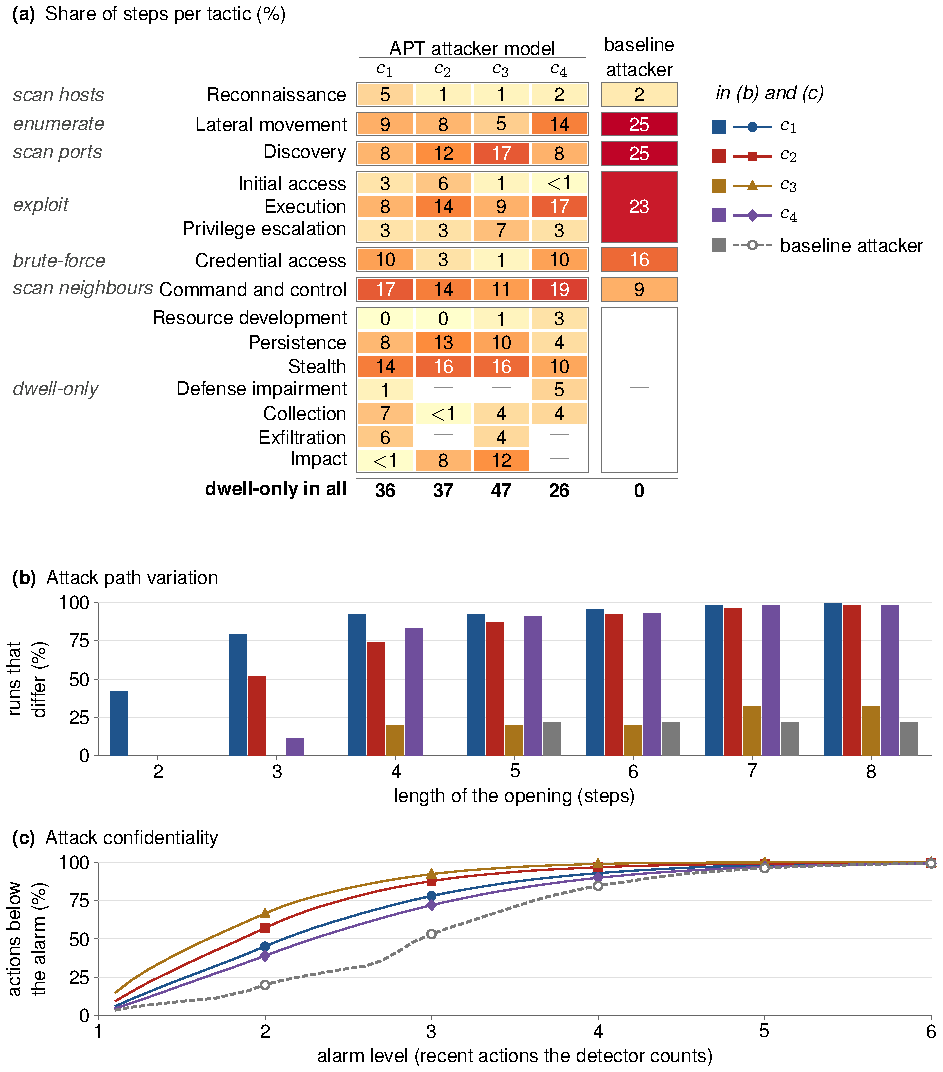
\includegraphics{fig_5-2-1a_campaign_openings}
  % 2026-10-02 (Marc: "if somebody just read the captions ... they could figure out what's happening";
  %  results_presentation_standard.md S4, I1-I3, T2, F5): caption rewritten to read the float alone,
  %  decoding only; metrics stay defined in Section 4.5. Session-written, DRAFT STATE --- ratify on read.
  \caption[How each attacker acts with no MTD running]{How each attacker acts with no MTD running: the APT attacker model on each attack profile $c_1$ to $c_4$, and the baseline attacker, over 1\,000 runs each (metrics in Section~\ref{subsec:metrics-behaviour}). A step is one tactic for the APT attacker model and one attack action for the baseline attacker. (a)~Relative tactic occurrence, the percentage of each attacker's steps taken in each tactic, on one colour scale, darker for a larger share; 0 is exact and $<$1 is above 0 but under 1. Rows are grouped by the attack action each tactic dispatches, named on the left (Section~\ref{subsec:tactic-verb-mapping}); an unmapped tactic dispatches none. The baseline attacker has no tactics, so its column gives the percentage of its steps in each attack action. A blank cell is a tactic the attacker does not have. (b)~Distinct attack paths among each attacker's 1\,000 runs, a path being the sequence of a run's first $k$ steps: 1 is every run opening alike, 1\,000 every run taking its own path; the baseline attacker takes 1 to 3. (c)~Attack confidentiality, higher for an attacker with fewer attack actions flagged by a scan detector that flags any attack action that is the fifth within 60\,s; the axis starts at 80\,\%, the dashed line is the baseline attacker, and the 95\,\% percentile bootstrap intervals over runs are narrower than the markers. The key above~(b) also serves~(c).}
  \label{fig:aio-coverage}
\end{figure}



% FIGURE 5.2 (fig:aio-divergence, the 4 x 4 pairwise-divergence matrix) DEMOTED
% TO BODY TEXT 2026-09-21 (Marc's ruling after the scrutinise-figure pass; record:
% results context §8d). Three independent reviewers converged: the figure
% re-expressed Figure 5.1(a) as one number per pair, its null was a floor that
% could not be failed, and it carried no scale. Under §3's test ("could this be
% false while every number stayed the same?") "every pair clears its null" is a
% construction fact: four nets with different tactic sets and weights give
% different pooled distributions, and a split-half null over ~50 000 steps per
% profile shrinks with the corpus (at a thousand seeds the ratio grows, no cell
% moves). Its generator panel and figure files are retired; the numbers below
% are the analyser's (data/results/ch5_s531_unopposed/numbers.json,
% core.divergence, printed by tools/ch5_unopposed_figures.py) and are
% PROVENANCE at 100 seeds --- re-derive at the reported count before citing.
% DENOMINATOR RECONCILED the same day: the suite's divergence counted only
% records with a verb or a positive dwell, which dropped the zero-second
% resource-development entries on two profiles, so the cells were not computed
% over the shares Figure 5.1(a) prints. Now every record counts on both (a step
% is one tactic entered, the caption's own unit); ordering unchanged.
%
% CONTENT POINTS FOR THE T2 SENTENCES (Marc's prose; two sentences, after the
% reading of Figure 5.1(a)):
%  1. The measure, declared at first use (no chapter 2-4 antecedent for
%     "divergence"): the distance between two profiles' share-of-steps
%     distributions of panel (a), 0 for identical shares, 1 for no tactic in
%     common (squared Jensen-Shannon distance, base 2).
%  2. The range: every pair between 0.08 and 0.21; the closest pair is impact
%     and double extortion (0.077), the farthest double extortion and no
%     realised objective (0.207). Read on the 0-1 scale the four campaigns
%     largely overlap: the four hub tactics (command and control, stealth,
%     execution, discovery) carry about half of every profile's steps, so the
%     profiles are different weightings of one campaign vocabulary. That is T2's
%     honest form ("differently weighted campaigns"), not "different campaigns".
%  3. The noise floor, one clause: two random halves of one profile's runs
%     differ by less than 0.002 (ceilings 0.0003-0.0012), so every pair is at
%     least sixty times its noise. State as a clause, never as a test passed.
%  4. Presence against weighting, if wanted: tactics that only one profile of a
%     pair holds carry between a tenth and a half of each cell (0.09, 0.27,
%     0.35, 0.48, 0.51, 0.51); the impact tactic is the largest single term in
%     four of six pairs. This is what answers "just different tactic sets".
%  5. Double extortion sits nearer impact than exfiltration (0.077 against
%     0.142): an observation, marked, not explained (chapter 6).
% CEILINGS, for chapter 6 and not for this section:
%  - Mean divergence to the other three rises as a profile's flow count falls
%    (exfiltration 19 flows 0.124; impact 7, 0.128; double extortion 7, 0.142;
%    no realised objective 5, 0.156): the aggregate column's size confound,
%    weaker, inside the pairwise cells. "No realised objective is the most
%    distinct" is an ordering observation and may not be read as objective
%    conditioning.
%  - The size-matched label-blind control (the only instrument that separates
%    conditioning from corpus size, profile_divergence_findings.md §7) has NOT
%    run at L3. T2 carries the caveat until it does.
%  - "The one property shown to change an OUTCOME" may not be read from this
%    measure: on target reached (0.05-0.13) the profiles' intervals overlap, and
%    on hosts reached every ADJACENT pair is unseparated, though the ends are
%    not (impact 9.9 +- 0.9 against exfiltration 7.4 +- 0.6 and no realised
%    objective 7.2 +- 0.8; corrected 2026-09-21). A T4 fact for Table 5.3's
%    paragraph.
% TERMINAL-TACTIC HALF (where a run ends): clears its null on 3 of 6 pairs at
%  100 seeds, inside it on the rest; T4's paragraph, one clause, only if it still
%  fails at the thousand-seed rerun.

% REWORKED 2026-09-13 (stage-2 float audit, ch5 design handoff §18) --- the results-table genre (booktabs, grouped
% headers, intervals); gains the AGGREGATE row (the objective-conditioning
% contrast, read on outcome and behaviour measures) and the INHERITED row; the
% entropy column carries its hub-occupancy caveat as a footnote. A spacing
% (stealth) column WAITS on Marc's ruling on the axis-5 observation.
% POPULATED 2026-09-15 as a generated fragment (tools/ch5_unopposed_figures.py;
% caption lives in the fragment). Columns changed from the placeholder: the
% depth column is GONE (deepest successful stage reads 2.00 +- 0.00 on every
% profile under the partial mapping, and advance-after-first-success reads 1.00
% on every run --- both saturated, findings §6); successes per host, the
% axis-1 repetition measure, takes its place; target reached is a column,
% because under the targeted objective the profiles reach the database target
% unopposed in 5-17 % of runs at this horizon (the "reaches none" premise does
% not hold here). The stealth-spacing column still waits on C11.
% REWORKED 2026-09-21 (Marc's read and ruling; scrutinise-figure pass, results
% context §8e). The table has ONE job, takeaway T4: the no-defence reference, and
% that a fuller campaign is not a better outcome. It is now four of Table 5.2's
% effectiveness metrics, per attacker (blocked fraction is the fifth that reads
% with no defence, 0.24 in Table 5.4; it is structurally zero on the baseline), so
% every column is a term the reader has met and NO FOOTNOTE survives. CUT:
% distinct tactics and runs on the commonest opening (both repeat Figure 5.1),
% path entropy (its own footnote said not to read it), successes per host (a
% §5.4 metric, already in the cost table's no-defence rows, and printed "---"
% here for the baseline where that table prints 1.0), ended at time limit (one
% minus target reached; the limit is arbitrary). ADDED: delay to first
% compromise and runs with no compromise, the defended corpus's estimators, so
% "slower" is carried by a number. The aggregate STAYS (Marc: it is a profile).
% Rows are grouped under "movement attacker" so the profiles read as that
% attacker's, beside "baseline attacker". Blocked fraction is left out: it is
% structurally zero on the baseline attacker and is first read in §5.3.1.
% FAIRNESS, checked 2026-09-21: both attackers stop acting when a target host
% falls (the baseline's last record ends at that compromise in every run that
% reaches one; its termination_time reads the clock), so hosts reached and
% target reached are counted under one stopping rule. The old "ended at time
% limit 0.40" for the baseline was one minus runs that ended early, not a
% different rule. The pooled row of Table 5.4 agrees with these rows (hosts 8.1,
% delay 2 100 s, no compromise 0.04 over the four profiles).
% CONTENT POINTS FOR THE T4 PARAGRAPH (Marc's prose):
%  1. The ordering: the baseline attacker reaches about three times the hosts
%     (24 against 7-10), reaches the target in over half its runs (0.58 against
%     0.05-0.17), and compromises its first host about three times sooner
%     (about 700 s against 1 900-2 400 s).
%  2. The construction reason, if wanted: a profile's steps include tactics that
%     compromise no host and each carries a dwell time (chapter 4); the baseline
%     attacker's six activities all serve the next compromise. WHY the gap is
%     this size is not measured here and is chapter 6's.
%  3. Between profiles: target reached does not separate; hosts reached
%     separates impact from exfiltration and no realised objective only.
%  4. The exception, marked: double extortion never compromises a host in 0.08
%     of runs, the others in 0.00-0.05.
%  5. The hand-off: hosts reached at no defence is the denominator of
%     suppression (Table 5.2) in §5.3.
% SCRUTINY PASS 2026-09-21 (cold reader, context critic, numbers auditor,
% sceptical examiner; record: results context §8e). All 24 cells reproduce from
% the raw runs. What the pass adds to the content points above:
%  6. THE GAP IS READ AT THE 15 000 s TIME LIMIT AND DEPENDS ON IT. The same
%     corpus at 60 000 s (numbers.json, extension): target reached 0.58
%     exfiltration, 0.62 impact, 0.58 aggregate, 0.36 no realised objective,
%     against the baseline attacker's 0.67; hosts reached 17-21 against 25. So
%     "a fuller campaign is not a better outcome" FAILS the §3 test as worded
%     (move the limit and it reverses). T4's honest form: at this time limit
%     the movement attacker has reached less, because it is slower; chapter 4
%     declares the dwell times as inputs, so the pace is a construction fact
%     and may be given as the reason. RULING OWED from Marc on T4's wording
%     and on whether the 60 000 s reading enters the table, the body text or
%     neither (Table 5.1 does not declare 60 000 s; C36).
%  7. DOUBLE EXTORTION STALLS and is not merely slow: at 60 000 s it still
%     reads 9.2 hosts, target reached 0.05 and 0.08 of runs with no
%     compromise, while its steps per run rise from 454 to 1 742. Exception,
%     marked and not explained; the cause is chapter 6's. It sits inside the
%     pooled denominator of every suppression figure.
%  8. "Three times sooner" is on means; the delay is skewed (exfiltration mean
%     2 397 s, median 1 667 s; baseline 675 against 631), so on medians it is
%     about 2.6 times. Say "mean" or quote the median.
%  9. The delay is over the runs that compromise a host (92-100 of 100 on the
%     profiles, 100 on the baseline). Counting the others at the limit would
%     move double extortion from fastest to slowest; the ordering AMONG
%     profiles on this column is therefore not read.
% 10. The aggregate's 0.17 is not separated from the profiles at 100 runs (four
%     runs above impact); one clause, no marker in the table.
% 11. The 0.02 of baseline runs that end on the inherited compromise-ratio stop
%     are not counted as target reached, on either attacker (the movement row
%     now applies the same filter; it changes nothing at 15 000 s).
% 12. RULED 2026-09-21 (Marc): T4 takes the pace form; hosts reached carries
%     "(of 50)"; double extortion is an exception here and chapter 6's to
%     discuss. MEASURED for his question "does the baseline attacker give up":
%     yes. On the 60 000 s runs its hosts reached is flat at 25.2 from 20 000 s
%     (24.3 at 15 000 s); where it never holds a target its last compromise is
%     no later than 19 346 s. The movement attacker is still climbing at
%     60 000 s (exfiltration 7.4 / 12.8 / 17.2 at 15 000 / 30 000 / 60 000 s).
%     So the time limit reads one attacker nearly finished and the other about
%     a third of the way. RULED 2026-09-22 (Marc): A SENTENCE, not a figure.
%     One body sentence after the T4 ordering: with the runs extended to
%     60 000 s the baseline attacker adds no host after about 20 000 s, and the
%     movement attacker is still adding them at 60 000 s (17-21 of 50 on three
%     profiles and the aggregate; double extortion the exception). PREREQUISITE:
%     60 000 s is declared nowhere the reader has been (Table 5.1 gives 15 000 s
%     only, C36), so either Table 5.1 gains the extension or the sentence
%     declares it in passing ("in runs extended to 60 000 s").
% PROFILE CODES APPLIED 2026-09-22 (Marc's ruling): chapter 4 §4.3 now indexes
% the four as $c_1$ to $c_4$ and names the aggregate $c_{\mathrm{agg}}$; every
% chapter 5 float keys by code (tools/_ch5_style.py LABEL).
% REBUILT 2026-09-24 ON THE METRICS DESIGN (docs/handoffs/2026-09-22_metrics_provenance_and_instrumentation.md
% §4): Figure 5.1 is three panels, one per attacker-behaviour metric --- (a) time
% share per tactic with the baseline attacker's column, (b) attack path
% variation, (c) attack confidentiality --- and Table 5.3 carries ASP, NCR, MTTC
% and the attack rate. The content points in the comments above predate it and
% name the old columns; the body's four points are in that handoff's §4, and every
% number here is 100 seeds until the 1 000-seed run. An action, for the stealth
% pair, is a verb that runs: a blocked verb never touches the network
% (movement/attacker.py:896), and counting it would put c_4 level with the
% baseline attacker (numbers.json: attack_rate_counting_blocked); §4.5 states it.
% --- P2: Table 5.2. Placed BEFORE % GENERATED by tools/ch5_unopposed_figures.py from
%   data/results/ch5_s531_unopposed/numbers_reported.json (the no-MTD corpus,
%   1000 runs per attacker, 15000 s horizon). Do not hand-edit; regenerate.
% Rebuilt 2026-09-24 on the metrics design (Table 5.2's names and classes).
% 2026-09-30: MTTC at a target host (section 4.5.2, ruling H1), over the runs that take one.
% Caption session-written, how-to-read only. DRAFT STATE --- ratify on read.
\begin{table}[htbp]
  \centering
  \caption[Both attackers with no MTD running]{The attack outcome and the attack rate with no MTD running (Section~\ref{sec:evaluation-metrics}), for the APT attacker model on each attack profile $c_1$ to $c_4$ and for the baseline attacker, over 1\,000 runs each (Table~\ref{tab:experiment}). MTTC is taken over the runs that compromise a target host, whose share of all runs is the ASP: 42 to 139 runs per attack profile and 643 for the baseline attacker. Attack rate is per minute of simulated time. Brackets: a 95\,\% Clopper--Pearson interval; $\pm$: a 95\,\% interval on the mean (normal approximation). Each value is rounded to the precision of its interval.}
  \label{tab:unopposed-summary}
  \tablestyle
  \begin{tabular}{@{}lcccc@{}}
    \toprule
    Attacker & ASP & NCR & MTTC (s) & Attack rate (per minute) \\
    \midrule
    \grouprow{5}{APT attacker model} \\
    \quad $c_1$ & $0.12$ [$0.10$, $0.15$] & $0.149 \pm 0.004$ & $11\,300 \pm 500$ & $1.087 \pm 0.005$ \\
    \quad $c_2$ & $0.14$ [$0.12$, $0.16$] & $0.209 \pm 0.005$ & $10\,500 \pm 500$ & $0.888 \pm 0.006$ \\
    \quad $c_3$ & $0.06$ [$0.04$, $0.07$] & $0.172 \pm 0.006$ & $9\,700 \pm 900$ & $0.680 \pm 0.008$ \\
    \quad $c_4$ & $0.04$ [$0.03$, $0.06$] & $0.154 \pm 0.005$ & $10\,800 \pm 800$ & $1.228 \pm 0.009$ \\
    \midrule
    Baseline attacker & $0.64$ [$0.61$, $0.67$] & $0.496 \pm 0.012$ & $9\,000 \pm 200$ & $1.708 \pm 0.015$ \\
    \bottomrule
  \end{tabular}
\end{table}

%     (after the comment block that precedes it).
% REWRITTEN 2026-09-26 on Marc's read ("very rhetorically inflated ... literally we
%  just need to describe what's happening"; his step-through of every float is
%  the content, checked against the tracked numbers). Plain description: what the
%  float shows, the numbers that carry it, the APT property the metric records
%  (Table 3.2 via Section 4.5), a by-construction reason only where Marc gave one.
%  The agent draft it replaces is in git history (commit e83f280c). DRAFT STATE.
Table~\ref{tab:unopposed-summary} gives the attack outcome and the attack rate.
On each of $c_1$ to $c_4$ the APT attacker model achieves less than the baseline
attacker: its ASP is under a quarter of the baseline attacker's,
% [CONNECTIVE-PROSE PASS 2026-09-26, ch5 S12 two-fifths] 'at most
%  two-fifths' was false (c2: 0.199/0.487 = 0.41, numbers.json); the
%  numbers stated instead. SESSION-GENERATED on Marc's 2026-09-26 go-ahead
%  (docs/workflows/connective_prose.md; audit
%  docs/implementation/connective_prose_audit.md); prior text in git.
%  RATIFIED 2026-09-26 (Marc: 'I accept all this').
its NCR \prelim{0.14} to \prelim{0.20} against \prelim{0.49}, and its MTTC,
over the \prelim{5} to \prelim{13} runs in 100 that compromise a target host,
\prelim{11\,000} to \prelim{13\,000}\,s against \prelim{9\,000}\,s. Its pace is an
input: each step lasts the duration declared for its tactic
(Section~\ref{subsec:dwell-times}). Because a run ends when a target is taken,
\prelim{40}\,\% of the baseline attacker's runs last to the time limit, against
\prelim{87} to \prelim{95}\,\% of the APT attacker model's. Its attack rate is
lower by less, \prelim{0.70} to \prelim{1.24} attack actions per minute against
\prelim{1.71}. The model dispatches the simulator's attack actions in the order its
tactics call them, so \prelim{14} to \prelim{28}\,\% of the attack actions it dispatches
find a precondition unmet and fail before they run, and the attack rate does not
count them (Section~\ref{subsec:metrics-behaviour}). This follows from a design
choice of Chapter~\ref{ch:attacker-model}: the model reuses the simulator's six
attack actions (Section~\ref{subsec:tactic-verb-mapping}).

% GENERATED by tools/ch5_unopposed_figures.py from
%   data/results/ch5_s531_unopposed/numbers_reported.json (the no-MTD corpus,
%   1000 runs per attacker, 15000 s horizon). Do not hand-edit; regenerate.
% Rebuilt 2026-09-24 on the metrics design (Table 5.2's names and classes).
% 2026-09-30: MTTC at a target host (section 4.5.2, ruling H1), over the runs that take one.
% Caption session-written, how-to-read only. DRAFT STATE --- ratify on read.
\begin{table}[htbp]
  \centering
  \caption[Both attackers with no MTD running]{The attack outcome and the attack rate with no MTD running (Section~\ref{sec:evaluation-metrics}), for the APT attacker model on each attack profile $c_1$ to $c_4$ and for the baseline attacker, over 1\,000 runs each (Table~\ref{tab:experiment}). MTTC is taken over the runs that compromise a target host, whose share of all runs is the ASP: 42 to 139 runs per attack profile and 643 for the baseline attacker. Attack rate is per minute of simulated time. Brackets: a 95\,\% Clopper--Pearson interval; $\pm$: a 95\,\% interval on the mean (normal approximation). Each value is rounded to the precision of its interval.}
  \label{tab:unopposed-summary}
  \tablestyle
  \begin{tabular}{@{}lcccc@{}}
    \toprule
    Attacker & ASP & NCR & MTTC (s) & Attack rate (per minute) \\
    \midrule
    \grouprow{5}{APT attacker model} \\
    \quad $c_1$ & $0.12$ [$0.10$, $0.15$] & $0.149 \pm 0.004$ & $11\,300 \pm 500$ & $1.087 \pm 0.005$ \\
    \quad $c_2$ & $0.14$ [$0.12$, $0.16$] & $0.209 \pm 0.005$ & $10\,500 \pm 500$ & $0.888 \pm 0.006$ \\
    \quad $c_3$ & $0.06$ [$0.04$, $0.07$] & $0.172 \pm 0.006$ & $9\,700 \pm 900$ & $0.680 \pm 0.008$ \\
    \quad $c_4$ & $0.04$ [$0.03$, $0.06$] & $0.154 \pm 0.005$ & $10\,800 \pm 800$ & $1.228 \pm 0.009$ \\
    \midrule
    Baseline attacker & $0.64$ [$0.61$, $0.67$] & $0.496 \pm 0.012$ & $9\,000 \pm 200$ & $1.708 \pm 0.015$ \\
    \bottomrule
  \end{tabular}
\end{table}


% SPLIT 2026-09-24 from Figure 5.1 (Marc: "attack confidentiality is a bit constrained
% ... this needs to be a bit bigger so the reader can see"): the stealth reading
% (register E4) as its own float, full width. Generated by tools/ch5_unopposed_figures.py
% (emit_fig_c) from numbers.json core.metrics[*].confidentiality_over_run. Session-
% written caption, how-to-read only; DRAFT STATE --- ratify on read.
% --- P3: Figure 5.2, closing on the hand-off. Placed BEFORE \begin{figure} of
%     fig:aio-stealth; the \FloatBarrier before Section 5.3 keeps the float in 5.2.
% REWRITTEN 2026-09-26 on Marc's read ("very rhetorically inflated ... literally we
%  just need to describe what's happening"; his step-through of every float is
%  the content, checked against the tracked numbers). Plain description: what the
%  float shows, the numbers that carry it, the APT property the metric records
%  (Table 3.2 via Section 4.5), a by-construction reason only where Marc gave one.
%  The agent draft it replaces is in git history (commit e83f280c). DRAFT STATE.
% 2026-09-30 (Marc: attack confidentiality "as a panel (c)"): Figure 5.2 retired;
% the count-in-window detector of Section 4.5.1 gives one share per attacker
% (numbers.json core.metrics[*].attack_confidentiality). The owed figure is
% re-measured under that detector (dwell-only steps counted as actions: c1 0.77,
% c2 0.79, c3 0.83, c4 0.68; baseline 0.83). DRAFT STATE.
Figure~\ref{fig:aio-coverage}(c) shows attack confidentiality, the share of
attack actions a scan detector does not flag: \prelim{89} to \prelim{98}\,\% for $c_1$
to $c_4$, $c_4$ the lowest, against \prelim{83}\,\% for the baseline attacker.
Attack rate and attack confidentiality together record stealth
(Section~\ref{subsec:metrics-behaviour}), and the APT attacker model has the
lower attack rate and the higher attack confidentiality. The detector counts
attack actions, so the two are one observation. \owed{Counting the unmapped steps as
attack actions lowers the profiles' attack confidentiality to \prelim{68} to
\prelim{83}\,\%, at or below the baseline attacker's}{Section 5.2: attack
confidentiality with unmapped steps counted as attack actions was measured in a dry run
only; track it, or move the point to the limitations in Chapter 6}.


% ~1 unit. CARRIES PROPERTIES 6 and 7 --- the two declared capabilities,
% each reported against the null at which the run is bit-identical.
%  - P6 incentive-driven rationality, in Marc's terms (how long will it
%    keep going before a rational actor gives up, having spent much for
%    little): the disengagement frontier --- projected campaign effort
%    after each action, the effort at which it exceeds a patience budget,
%    mean abandonment effort against patience, per condition, with the
%    censoring fraction printed beside every point because the
%    conditional mean conditions on abandoning.
%  - P7 learning capability: breadth against the learning exponent, with
%    the decay as a second series.
% WHY THIS RUNG IS REPORTED AT ALL --- and the justification is deliberately
% NOT "the negative is a good result" (Marc, 2026-09-09: "don't put things in
% knowing the results, knowing that's going to be the strongest thing"). The
% ground is that a capability the model DECLARES must be reported against the
% setting at which it is inert, whichever way it falls, because a declared
% capability that is never measured is an assertion. That reason holds if the
% sweep comes back flat, positive or negative, which is the test.
% WHAT IS ON RECORD IS NOT YET WHAT THIS CHAPTER MAY SAY: the direction
% measured in 2026-08 predates d127f443 and its foundation may have moved (see
% the blocker below), so the prose commits to no direction until the
% pre-check runs. Marc's own read ("it doesn't really come through, but it's
% implemented") is the right register for the sentence either way.
% DEPENDS ON §4.3 RULING R3: without the history-term slot in the formal
% definition these two capabilities have NO ch4 antecedent, and two marks
% in tab:fidelity-verdict rest on mechanisms the dissertation never
% defines.
% FIGURES (2):
%  Fig. D  disengagement frontier: mean abandonment effort against
%          patience, one line per defence condition, censoring annotated.
%          PURPOSE: an attacker with a cost model quits, and when.
%  Fig. E  breadth against the learning exponent, series = decay rate,
%          null arm marked.
%          PURPOSE: the measured negative, and its shape.
%
% REVIEW PASS 2026-09-09 (third) --- THE HEADING, THE DIAL, AND A BLOCKER.
%
% HEADING RENAMED, Marc's to overrule ("declared capabilities --- I don't
% really understand that section"). "Declared capabilities" is repo
% vocabulary: it means the two things the attacker was GIVEN that it need not
% have had, each with a setting at which it is switched off and the run is
% bit-identical. In the chapter those two things are a sense of cost and a
% memory, so the heading now says that. Alternatives if this one does not sit
% right: "What the two optional capabilities buy"; "Cost and memory";
% "Giving the attacker a cost model and a memory". Heading conventions hold
% either way --- sentence case, no acronyms, declarative.
%
% "WE CAN DIAL THE ATTACKER'S PREDICTABILITY DOWN AND FIND A NICE BASELINE"
% (Marc, 2026-09-09). The dial exists and it is already in this subsection
% under another name: lambda, the rationality exponent in the utility
% modulator. It exponentiates each transition's utility RATIO against the
% out-set mean, so at lambda = 0 every factor is 1.0 and the run is
% bit-identical to no modulator at all, and as lambda rises the routing
% concentrates on the high-payoff moves. Concentrating the routing IS making
% the attacker more predictable --- so ONE SWEEP CARRIES TWO READINGS, and
% the second is free: at each lambda, report effective behavioural breadth
% beside the outcome measure. The uniform-weight arm is the other end of the
% same axis (maximum variety, no corpus preference).
% THAT ALSO GIVES THE "NICE BASELINE" A CRITERION INSTEAD OF A FEEL: the
% operating point is the largest lambda at which behavioural breadth is still
% plural --- goal-directed without collapsing to one path. Report it that
% way and the choice of lambda stops being a declared value and becomes a
% selected one, which is the same move sec:sensitivity makes.
% WHAT IT IS NOT: a game-theoretic equilibrium. There is no second player
% optimising against this attacker --- the defender is frozen on a schedule
% --- so the word "equilibrium" must not appear. It is an operating point.
%
% BLOCKER, NEW AND NOT ON THE CHAPTER'S LIST: THE LEARNING NEGATIVE IS A
% PRE-RESTORATION RESULT WITH A NAMED REOPENING CONDITION, and Fig. 5.9's
% caption currently states it as settled fact. Every exploit-learning number
% predates d127f443, and that commit changed exactly the channel this
% capability probes --- D-19 reinstated the OS-gated exploit-success channel,
% so OS-dependent vulnerabilities now fail on a mismatched host. The 2026-08-11
% null rests on a PERFECT-EXPLOIT CEILING: when a roll always succeeds, no
% exploit-phase capability has headroom, so of course the learner buys
% nothing. If the OS gate now refuses a material fraction of this attacker's
% exploits, that ceiling has dropped and the learner has headroom it did not
% have when it was measured. The original sweep also moved only
% `services_per_os` and never the OS pool, which D-19 has made a live lever.
% THE CHEAP PRE-CHECK, and it decides the whole question: measure the
% movement arm's exploit-success rate on ONE no-MTD cell on the restored
% substrate. If the gate refuses little, the null stands as written and the
% caption is safe; if it refuses much, the negative is re-tested (about 370
% runs) with the OS pool as a second lever before any sentence here claims it.
% Until that pre-check runs, Fig. 5.9 states a negative measured on a
% substrate that no longer exists.
% ---------------------------------------------------------------------
% REVIEW PASS 2026-09-09 (fourth): THIS IS THE ABLATION SUBSECTION, and it is
% widened to be one. Marc: "we're not looking at the baseline as a sort of
% ablation study, and that should be a part of it --- so we can look at the
% aggregate. How would you fold that in? I don't know if you need a specific
% ablation section, I don't know how they do it."
%
% HOW THEY DO IT. A titled ablation subsection has a LOCAL precedent and it is
% the strongest convention signal available: Tay's evaluation chapter carries
% an explicit ablation subsection, in this supervisor's own lineage, so the
% examiner has seen the form. He 2025 does the same for a structural property
% of its defence. The journal corpus mostly does not ablate at all, so there is
% no competing convention to weigh against it.
% THE ANSWER IS THEREFORE: NO NEW SECTION, BUT THIS ONE IS RENAMED AND WIDENED.
% It already held two arms against their nulls; it now holds all five, which is
% its natural content and costs no unit. That also removes a duplication ---
% tab:parameter-register carries "the five optional capabilities" as ONE swept
% row pointing here, rather than five rows the ladder repeats.
%
% WHY AN ABLATION EARNS ITS OWN SUBSECTION ON MERIT, not on what it returns:
% sec:effectiveness and sec:efficiency ask what the DEFENCE does; an ablation
% asks what a COMPONENT OF THE ATTACKER contributes. That is a different
% question with a different comparison (against a null, not against no
% defence), and scattering the answers across the strands means the ladder is
% never seen as a ladder. In practice the five share one apparatus --- same
% arms, same null convention, same table --- so reporting them together is
% cheaper in words than reporting them five times in five places.
%
% THE LADDER, most capable first. Each rung switches ONE thing off, and every
% null is a setting at which the run is bit-identical, which is what makes the
% comparison a measurement rather than a re-implementation:
%   full model                         all five on
%   - cost sensitivity                 the rationality exponent at 0
%   - within-run learning              the learning exponent at 0
%   - outcome-conditioned routing      the verdict-blind arm (used as the
%                                      control in subsec:aio-disruption; it is
%                                      reported here as a rung, cross-referenced
%                                      there, not measured twice)
%   - corpus-derived preference        uniform branching weights
%   - OBJECTIVE CONDITIONING           the AGGREGATE ENVELOPE
%
% THE AGGREGATE IS THE RUNG MARC IS ASKING ABOUT, and placing it here fixes a
% mis-filing. `aggregate` is the FLOW UNION --- the same corpus with the
% objective partition switched off, and the divergence record's own figure
% legend calls it "unsegregated". That makes it the null for the model's
% CENTRAL claim, objective conditioning, in exactly the way the exponent at 0
% is the null for cost sensitivity. It currently rides the hypothesis tree as
% characterisation (C-agg) rather than as an ablation arm, and the tree's own
% open ruling 5 --- is the claim over four profiles or five --- is this same
% question asked from the other end. Reading it as a rung answers both.
%   ONE CAVEAT TRAVELS WITH IT, and it is pre-registered rather than
%   discovered: the DIVERGENCE-TO-AGGREGATE column may not be read as objective
%   conditioning. Its kill criterion fired at Spearman -1.0 against flow count,
%   because `aggregate` is the union and a large class is close to the union by
%   arithmetic. The arm is fine; that one statistic is not. Read the aggregate
%   rung on outcome and behaviour measures --- breadth, coverage, blocked
%   fraction --- never on its distance to the union.
%
% AND ONE SENTENCE THAT PROTECTS subsec:eff-cross-arm: THE INHERITED ATTACKER
% IS NOT A RUNG ON THIS LADDER. It is not this model with everything switched
% off --- it is a different machine (a deterministic policy over six verbs,
% with no net, no objective and no routing decision to condition), and no
% setting of any parameter reaches it. So a cross-arm difference is NOT
% attributable to any one component, and the chapter must not let the ablation
% ladder and the cross-arm comparison be read as the same instrument. Saying
% that once, here, is what earns the cross-arm claim its narrower and correct
% form: the two attackers depend on different substrate properties, which is a
% structural statement, not a component-wise one.
%
% FIGURE AND TABLE FOR THE WIDENED SUBSECTION: the two figures already placed
% stay (they are the two rungs with a continuous dial, so they are the two that
% have a shape to draw), and the ladder as a whole becomes a small table ---
% rung, what is switched off, the setting at which it is inert, the effect.
% The three discrete rungs are table rows; a figure each would be three
% two-bar charts.
% ---------------------------------------------------------------------
% REMOVED 2026-09-13 (design C31, Marc: "ablation is going"): the subsection
% "What each part of the model contributes" (label subsec:aio-capabilities) with
% fig:aio-disengagement, fig:aio-learning and tab:ablation-ladder. The journal
% corpus does not ablate; Tay's subsection served an RL agent. What survives:
% the aggregate envelope as a row of tab:unopposed-summary (the objective-
% conditioning contrast), the verdict-blind arm as subsec:aio-disruption's
% control, and the cost/learning modulators at their inert defaults as rows of
% tab:factors-fixed. CONSEQUENCE, flagged for Marc's confirmation: the two
% fidelity-verdict marks for cost sensitivity and learning drop to implemented,
% not evidenced. The retired comment blocks (the lambda operating-point idea,
% the learning pre-check blocker, the ladder) are in git history and the ch5
% design handoff §10.4, §11.1, §16.

% SUPERSEDED IN SHAPE 2026-09-23 (register E1, Marc's heading rulings): this is
% phase two, the APT attacker model under MTD with the baseline attacker as the
% reference line; effectiveness and efficiency merged, subsections by the purpose
% of each experiment. The three-section separation argued below (attacker /
% defences / cost) is overturned; the comments stand as the trail.
% 3 units, one per subsection. THE MTD EVALUATION PROPER: what the
% defence achieves, on the inherited suite's own effectiveness axis
% (Table 3.1) --- success events, attacker time, attack paths, system
% state. Reported against the no-defence denominator of
% sec:attacker-in-operation.
%
% THE GRAMMAR OF EVERY RESULTS PARAGRAPH HERE (conventions e), four
% moves in order: the observation, as ordering or trend (magnitude as a
% relative percentage where it is carried); the mechanism, in the next
% sentence, as the reason --- flagged "we hypothesise" where it was not
% measured, never stated as a finding; the exception or surprise, marked
% as such; the conditional recommendation closing the subsection.
% Declare the success criterion AT THE METRIC, before the result, with a
% one-sentence justification (He's form) --- that is where the retired
% grading vocabulary now lives, a sentence at the definition site rather
% than a unit of its own. Where a separation is real but small, defer
% materiality to the reader explicitly (Outkin's form) rather than
% inflating it.
%
% BLOCKED, and it blocks prose not shape: internal MTTC ranks the
% mechanisms perversely and is the project's named primary metric; its
% brief is owed before this section names it. Cross-arm event counts are
% inflated ~3.75x by per-vulnerability row writing; the corrected counter
% exists.
%
% REVIEW PASS 2026-09-09 (third) --- WHAT THIS SECTION IS, because the reading
% it invites is the wrong one. Marc read it as "basically just pure runs ---
% how effective are the profiles running unopposed". That is sec:attacker-in-
% operation, which now sits immediately above it and takes the unopposed arm.
% THIS section runs the DEFENCES. Every number in it is a difference from the
% no-defence reference that §5.3 fixed, and the object being evaluated here is
% the defence, not the attacker.
% THE ONE-LINE SEPARATION, worth putting in the roadmap sentence so no reader
% makes the same read: §5.3 asks what the attacker does; §5.4 asks what the
% defences do to it; §5.5 asks what that costs, on both sides.
% THE ORDER IS THE FUNNEL and it is deliberate: characterise on the undefended
% target, prune to what matters, then evaluate the defence against that with
% the pruning rule stated (He 2025). It is also what makes §5.3 a step in the
% argument rather than a detour --- state the rule explicitly, because the
% reason breadth rather than objective achievement is the denominator is a
% FACT FROM §5.3 (the profiled attacker reaches the mass objective in none of
% its unopposed runs) and not a preference.
\FloatBarrier
\section{APT attacker model versus MTD}
\label{sec:effectiveness}

% DRAFT STATE 2026-09-25 --- agent-drafted on Marc's request ("each of the agents will
%  do each of the prose elements"); slot plan: handoff 2026-09-25_ch5_setup_defence_and_prose_slots.md
%  Part C D2 (the §5.3 preamble). Ratify on read.
%  Slots -> sentences: P1 -> s1; P2 -> s2; P3 -> s3; P4 -> s4; roadmap (P5's order half;
%   the 200 s half is carried by §5.1's Defence unit and not repeated) -> s5.
%  Pooling verified: analyse.py _pool() concatenates the runs of FOUR = c1..c4 (equal
%   run counts, so equal weight); the aggregate is never pooled. disruption.py load()
%   skips profile "aggregate", so §5.3.1 (fig:aio-adaptivity, "four attack profiles
%   pooled") pools the same way; c_agg appears only in fig:eff-suppression-profiles and
%   fig:eff-schemes-profiles (§5.3.3), which draw each profile, not the pool.
%  Terminology: "reference" kept for the no-defence runs only (§5.1; conventions §f2,
%   coordinator correction); the baseline attacker is "beside it for comparison".
%  Numbers: none typed (95\,\% is §4.5.4's declared level, not a result).
% REWRITTEN 2026-09-26 on Marc's read ("very rhetorically inflated ... literally we
%  just need to describe what's happening"; his step-through of every float is
%  the content, checked against the tracked numbers). Plain description: what the
%  float shows, the numbers that carry it, the APT property the metric records
%  (Table 3.2 via Section 4.5), a by-construction reason only where Marc gave one.
%  The agent draft it replaces is in git history (commit e83f280c). DRAFT STATE.
% [CONNECTIVE-PROSE PASS 2026-09-26, ch5 U5 5.3 preamble] S1 restated the
%  heading, S2 the float layout every caption states; replaced by the one
%  frame fact 5.3 needs (4.5.3's own wording), which carries the link cut
%  from the 5.2 close. SESSION-GENERATED on Marc's 2026-09-26 go-ahead
%  (docs/workflows/connective_prose.md; audit
%  docs/implementation/connective_prose_audit.md); prior text in git.
%  RATIFIED 2026-09-26 (Marc: 'I accept all this').
Every effect is taken against the same attacker's no-MTD runs of Section~\ref{sec:attacker-in-operation}. Where the APT attacker model is one
line or column, it pools $c_1$ to $c_4$ with equal weight.
% [CONNECTIVE-PROSE PASS 2026-09-26, ch5 U5b rule] The decision rule
%  declared in the word the body uses ('told apart'). SESSION-GENERATED on
%  Marc's 2026-09-26 go-ahead (docs/workflows/connective_prose.md; audit
%  docs/implementation/connective_prose_audit.md); prior text in git.
%  RATIFIED 2026-09-26 (Marc: 'I accept all this').
An effect is told apart from zero when its 95\,\% interval excludes zero, and MTD mechanisms and deployment strategies that
share a Scott--Knott rank are not told apart
(Section~\ref{sec:dimensions}).
Section~\ref{subsec:aio-disruption} shows what a single deployment does to each
attacker, Section~\ref{subsec:eff-cross-arm} the NCR and ASP reductions of each MTD mechanism and deployment strategy
across the deployment interval, and Section~\ref{subsec:eff-under-defence} the
same by mechanism, attack profile and deployment strategy.

% ~1 unit. CARRIES PROPERTY 4 (adaptivity), which is the one property
% that cannot be read from the unopposed arm, because it is definitionally
% about what changes when the defence bites.
%  - action mix in the n visits before against the n after each mutation
%    (paired within run, so seed variance cancels);
%  - recovery time from a mutation to the next success, censoring stated;
%  - failure-conditioned routing rate, correlated with breadth;
%  - the verdict-blind ablation as the control: the same runs with the
%    routing made blind to the environment's verdict.
% The honest reading on record: the loop demonstrably operates and has
% not been shown to change an outcome. Report it that way.
% FIGURES (1):
%  Fig. C  action mix before against after a mutation, paired bars by
%          verb or place class, movement arm and the verdict-blind
%          control side by side.
%          PURPOSE: the attacker measurably does something different
%          after being disrupted, and the control shows the difference is
%          the verdict-conditioning rather than drift.
%
% REVIEW PASS 2026-09-09 (third) --- TWO ANSWERS THIS SUBSECTION OWED MARC.
%
% "WHAT AXES OF DISRUPTION ARE WE GOING TO DO --- WHICH MECHANISM, DIVERSITY
% OR SHUFFLE?" The chapter never said, and it has to. The answer is not "all
% seven": this subsection is about the ATTACKER's response, so it wants the
% smallest condition set that spans the ways a defence can reach it, and that
% set is already established rather than chosen here.
%   THE SPANNING SET IS A 2 x 2, on ATTACKER-FACING EFFECT rather than on the
%   shuffle/diversity taxonomy of Table 2.4. The two axes are the resource
%   LAYER the mechanism rewrites, because that is what decides whether the
%   attacker's state survives:
%     network layer -> SEVERANCE. Clears the host cursor, destroying position.
%       Blocked fraction 0.15 -> 0.72. The two network-layer mechanisms are
%       ONE attacker-facing effect (0.721 against 0.725), so running both buys
%       nothing except the evidence that they are one effect --- which is
%       itself worth one sentence.
%     application layer -> SURFACE RE-ROLL. Re-rolls the vulnerability set on
%       uncompromised hosts. Barely reaches this attacker (blocked fraction
%       stays at the no-defence ~0.16) because exploitation is uninterruptible
%       on that arm (D-35).
%   SO: one network-layer mechanism and one application-layer mechanism span
%   the effect space for this subsection, with the no-defence arm as the
%   origin. Everything else is sec:effectiveness's job, where the full
%   condition set belongs.
%   THE SDR CLASSES DO NOT SPAN IT, and that is a finding rather than a
%   convenience: MTDSim has two of the three SDR families (no redundancy,
%   ch2), and shuffle spreads across BOTH layers while diversity sits in one,
%   so the taxonomy the literature reads by and the taxonomy the attacker
%   feels are not the same partition. Say that once; it is the cheapest form
%   of the state-bounds argument the discussion carries.
%   THE THIRD AXIS IS TEMPO, not a mechanism. The mutation interval is the
%   dimension along which "disruption" varies continuously, and it is where
%   the discrimination gate bites. If this subsection shows a response AT ALL,
%   it should show it at two tempos, because a response that only exists at
%   one interval is a property of the interval.
%   THE PURE-INTERRUPT PAIR is the free extra, already noted in the discussion
%   notes: IP shuffle and port shuffle reach the attacker through their class's
%   INTERRUPT ALONE --- no state rewrite it can read --- so the pair prices
%   what an interrupt by itself is worth at each layer. It is the cleanest
%   available isolation of the disruption channel and it costs no new runs.
%
% "ACTION MIX --- I DON'T REALLY UNDERSTAND THAT." Fair, and the phrase is
% jargon that has leaked from the measurement suite into the chapter. What it
% is, in one sentence: WHAT THE ATTACKER IS DOING CHANGES AFTER IT IS HIT.
% Take the handful of steps immediately before each mutation and the handful
% immediately after, and compare which activities fill them --- more
% reconnaissance and less exploitation after a mutation would be the attacker
% re-orienting. It is paired inside each run, so run-to-run variation cancels;
% the verdict-blind arm is the control that says the change is a response and
% not drift. In the prose, describe it that way and never as "action mix".
% OWED HERE, 2026-09-20 (setup handoff §AL3, §AM P10): the verdict-blind control
% is run (run_corpus.py "blind" group) and declared nowhere; §5.2 does not carry
% it, so it is declared at this subsection's head, where it is first used.
\subsection{Response to disruption}
\label{subsec:aio-disruption}

% DRAFT STATE 2026-09-25 --- agent-drafted on Marc's request ("each of the agents will
%  do each of the prose elements"); slot plan: handoff 2026-09-25_ch5_setup_defence_and_prose_slots.md
%  Part C D3 (S31-h ... S31-close), content = results-context §8g-5 takeaways R1-R3 as
%  amended (the second table). Ratify on read.
%  PLACEMENT: PART 1 replaces everything between \label{subsec:aio-disruption} and
%  \begin{figure}[H] of fig:aio-adaptivity (the 2026-09-22 HEAD DECLARATION comment
%  and its paragraph are retired; the figure-history comments are carried forward
%  verbatim below the new head). PART 2 goes immediately after \end{figure} of
%  fig:aio-adaptivity, before the "~1 unit. THE THESIS'S OWN CLAIM" comment block
%  that belongs to subsec:eff-cross-arm.
%  Head repairs (D3 i-iii): (i) the control declared with its true scope, IP shuffle
%  and OS diversity only (run_corpus.py group "blind"), and its tracked result
%  reported, on the measure it was read on (choice 3 of the element brief: no
%  control result exists on the NCR growth rate or time lost; the tactic-level
%  read in numbers.json s522 is tracked); (ii) no token / routes / identity: stated
%  in chapter 4's words (failure matrix, base weights, verdict, step, precondition);
%  (iii) "grouped by the layer each rewrites" dropped: panel (c) is per mechanism.
%  Slots -> sentences:
%    S31-h   head s1 (why here), s2 (which interval, pointed to Section 4.5),
%            s3 (200 s, one sentence), s4-s5 (the control and its result)
%    S31-a+b body 1 s1 (R1, the exception marked in its last clause, not explained)
%    S31-c   body 1 s2 (R2, as an ordering)            S31-e  body 2 s1 (R3)
%    S31-d   body 2 s2, \owed (ch2 placeholder item (ii) not landed)
%    S31-close body 2 s3
%  Coordinator correction applied: "reference" is not used (reserved for the no-defence runs).
%  Numbers (100 seeds; every one \prelim):
%    4 %   <- disruption_numbers.json reads["movement|host|200"].pre_rate_per_ksec 0.0240
%             / none_rate_per_ksec.movement 0.5543 = 4.3 %
%             (the baseline attacker's counterpart, 18 % before a service-layer
%             deployment, reads["baseline|service|200"], was cut for budget)
%    0.025 <- numbers.json s522.conditions["ip_shuffle|2000"|"os_diversity|2000"]
%             .movement/.control.refused_by_offset[-5..+5].blocked; max |diff| 0.0234
%             (IP shuffle), 0.0237 (OS diversity). At 200 s IP shuffle it is 0.029,
%             so the sentence leans on the head's "read at 2 000 s"; the window is
%             disruptions (interrupts), not every deployment, and the four profiles pooled.
%    "every mechanism except user shuffle" (six of seven per attacker)
%          <- reads[*|<mechanism>|2000].relative_pct[6] (first bin after): model
%             7/10/10/64/81/63 %, baseline 22/56/44/25/32/15 %; user shuffle 113 % / 96 %
%    R2 as an ordering (magnitudes cut for budget and the one-or-two-magnitudes rule;
%    the figure's (a)/(b) carry them): IP shuffle, model still at 76 % in the bin
%    +1 000..+1 125 s (reads["movement|ip_shuffle|2000"].relative_pct[14]) while the
%    baseline is at 22 % then 101 % (reads["baseline|ip_shuffle|2000"].relative_pct[6..7]);
%    "the order reverses" <- reads["baseline|service_diversity|2000"].relative_pct[15]
%             = 72 % in the last bin (+1 125..+1 250 s); reads["movement|service_
%             diversity|2000"].relative_pct[6..11] = 63, 74, 81, 72, 84, 97 %
%             (the R2 magnitudes 72 % / ~700 s cut for budget; the figure shows them)
%    429, 511 <- reads["movement|complete_topology|2000"].time_lost.seconds 428.6,
%             reads["movement|ip_shuffle|2000"].time_lost.seconds 510.8
%    593   <- reads["baseline|service_diversity|2000"].time_lost.seconds 592.8
%    "its only interval to exclude zero" <- baseline time_lost.lo < 0 on the other six
%             (IP -40, complete -13, host -28, port -126, OS -111, user -75)
%  Constants, not corpus numbers (no \prelim): 2 000 s, 200 s, 125 s bin, 1 250 s
%  window (Section 4.5; Table 5.1).
%
% ---------------------------------------------------------------- PART 1 (head)
% REWRITTEN 2026-09-26 on Marc's read ("very rhetorically inflated ... literally we
%  just need to describe what's happening"; his step-through of every float is
%  the content, checked against the tracked numbers). Plain description: what the
%  float shows, the numbers that carry it, the APT property the metric records
%  (Table 3.2 via Section 4.5), a by-construction reason only where Marc gave one.
%  The agent draft it replaces is in git history (commit e83f280c). DRAFT STATE.
Adaptivity, the attacker's response to a deployment
% [CONNECTIVE-PROSE PASS 2026-09-26, ch5 S3 one property] 'the one
%  property' was false by Table 3.2: learning and scheme awareness also
%  need a defence. SESSION-GENERATED on Marc's 2026-09-26 go-ahead
%  (docs/workflows/connective_prose.md; audit
%  docs/implementation/connective_prose_audit.md); prior text in git.
%  RATIFIED 2026-09-26 (Marc: 'I accept all this').
(Table~\ref{tab:attacker-properties}), is a property that needs MTD to be seen. Attack actions blocked per MTD deployment and time lost per MTD deployment record it
(Section~\ref{subsec:metrics-effectiveness}). Both are read at the 2\,000\,s deployment
% [CONNECTIVE-PROSE PASS 2026-09-26, ch5 S4 recovered] Attribution beyond
%  measurement, contradicted by the chapter's own number (the baseline
%  attacker is back to its rate within 250 s); the by-construction reason
%  (4.5.3's window) stated instead. SESSION-GENERATED on Marc's 2026-09-26
%  go-ahead (docs/workflows/connective_prose.md; audit
%  docs/implementation/connective_prose_audit.md); prior text in git.
%  RATIFIED 2026-09-26 (Marc: 'I accept all this').
interval: at 200\,s the next deployment comes 200\,s later, which caps the time lost at 200\,s.
% [2026-09-26: the owed control sentence RESOLVED by Section 5.4, which reports
%  the control on the metrics Section 4.5 defines (time lost per MTD deployment
%  among them) and is listed in Table 5.1's Arm row. Closes handoff
%  2026-09-25_ch5_setup_defence_and_prose_slots.md item B4, option (a).]
Section~\ref{sec:ablation} tests whether the failure matrix contributes to this
response.

% ---- Figure-history comments, carried forward verbatim (dissertation.tex l.7387-7450):
% REWORKED 2026-09-13 (stage-2 float audit, ch5 design handoff §18) --- grouped bars in a 2 x 2 of lettered panels
% (mechanism x tempo), the control as a series beside the treatment, legend
% once. The spanning pair and two tempos are the ruled content of this
% subsection (handoff §10.2); a response shown at one interval is a property
% of the interval. Dense by design, so the family rule applies if it does not
% read: split into two figures at descending abstraction rather than shrink.
% POPULATED 2026-09-17 (tools/ch5_adaptivity_figure.py): the verb-level activity
% mix, 2 x 2 mechanism x interval, control beside the treatment. A null on the
% record (findings §4), and Marc's read 2026-09-22 upheld: four panels that
% look the same, no visible response, and the WRONG RESOLUTION --- the verb is
% downstream of the tactic-to-verb mapping, so a verb-level mix inherits the
% baseline attacker's shape by construction. That result is now one body
% sentence here and a limitation for chapter 6.
% REDESIGNED 2026-09-22 (results context §8g, takeaways T5-T8 ratified; tools/
% ch5_disruption_figure.py from numbers.json §s522, the same corpus, the read in
% ch5_s532_adaptivity_findings.md §7). Read at the tactic-level record. The
% mechanism fact the redesign rests on, verified from code: the baseline
% attacker is restarted in a phase set by the mechanism's layer (host layer ->
% scan host, service layer -> scan port, credentials -> exploit), whatever
% phase it was in; the movement attacker's token is never moved --- the
% disruption is a failure verdict at the place it is on, and that place's
% failure row routes it. The layer shows underneath: after a host-layer
% mechanism every verb that acts on the current host fails its precondition
% until an enumerate or scan host succeeds.
%   (a) the response: share of visits with a failed precondition, five visits
%       either side of a disruption, per layer, at 2 000 s (at 200 s the next
%       disruption lands before the last is recovered from, so the share sits
%       near one half throughout: a sentence, not a panel);
%   (b) the recovery: time to the next compromise per layer, both attackers,
%       censored share printed, each attacker's own unopposed gap between
%       compromises as the dashed reference (the pace anchor).
% NOT DRAWN, one sentence each (numbers in §s522): the position by lifecycle
% stage is unchanged either side of a disruption (JSD <= 0.004; the token
% does not fall back a stage); the control (routing on the base proportions
% whatever the verdict) tracks the model within 0.025 at every step, so T7 is
% a sentence; the credential layer disrupts the attacker 0.1 times per run at
% 2 000 s; the baseline restarts in the layer's phase in every disruption but
% the run-ending ones. Caption session-written, DRAFT STATE --- ratify on read.
% The control's declaration at the head of this subsection is still owed.
% RULED 2026-09-22 (Marc, third scrutinise round, results context §8g): panel
% (b) in the RATIO form --- each bar a multiple of that attacker's own mean gap
% between compromises with no defence, a seeded bootstrap interval on the
% ratio, a hollow circle at each mechanism of the layer alone --- because the
% absolute form read as pace (T4) to three cold readers and the figure's job is
% the layer dependence and the contrast in kind. The absolute times (2 051 and
% 1 531 s against 1 291 s; 425 and 575 s against 394 s) are body-text facts.
% The layer-level inversion is an observation for the movement attacker in
% every condition and a one-condition fact for the baseline attacker (service
% diversity 2.42x; port shuffle and OS diversity at its pace): the body must
% say so, or the layer bar reads as a false aggregate.
% REBUILT 2026-09-24 (Marc: "almost a complete write-off ... go back to the
% basics"; "less is more"; every axis a defined metric; both attackers measured
% by one rule). Takeaways R1-R3 and the full record: results context handoff
% §8g-5. Data: data/results/ch5_defended/disruption.py -> disruption_numbers.json;
% generator tools/ch5_disruption_figure.py. (a) NCR growth rate around a
% deployment, relative to the attacker's own rate in the 750 s before (both
% attackers anchored on the moment the rewrite lands, every deployment counted);
% (b) time lost per deployment, per mechanism = the area of (a)'s dip, as seconds
% at the attacker's own pace. The per-layer read of (a), the 200 s rates, the
% refused-action share, the baseline's restart rule and the control are body
% sentences (content points in §8g-5). "Time lost" replaces "recovery time"
% (the quantity changed: the per-event wait to the next compromise failed on
% censoring and on an unmatched reference) --- Marc's to overturn. Caption:
% how to read it, no result. DRAFT STATE --- ratify on read.

\begin{figure}[tp]
  \centering
  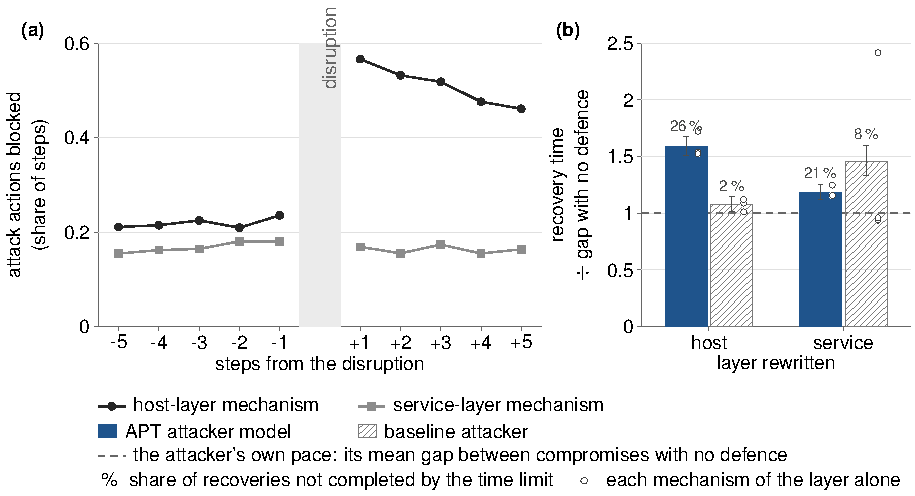
\includegraphics{fig_5-2-2a_disruption_response}
  % 2026-10-02 (Marc: "if somebody just read the captions ... they could figure out what's happening";
  %  results_presentation_standard.md S4, I1-I3, T2, F5): caption rewritten to read the float alone,
  %  decoding only; metrics stay defined in Section 4.5. Session-written, DRAFT STATE --- ratify on read.
  \caption[What an MTD deployment costs each attacker]{What an MTD deployment costs each attacker: each MTD mechanism deployed alone every 2\,000\,s, against the APT attacker model, its attack profiles $c_1$ to $c_4$ combined (solid; 4\,000 runs, 1\,000 per attack profile) and against the baseline attacker (hatched; 1\,000 runs), grouped by what each reconfigures. (a)~Attack actions blocked per MTD deployment: 1 when every deployment disrupts an attack action, 0 when none does. A deployment's layer, not its mechanism, decides which attack actions it can disrupt (Section~\ref{subsec:attacker-model}), so the mechanisms of one layer block nearly the same share. (b)~Time lost per MTD deployment: the delay to the attacker's next compromise against the same seed with no MTD; below zero, the next compromise came sooner. A disrupted attack action need not delay the next compromise, so a mechanism can block every attack action in~(a) and still not delay the next compromise in~(b) (Section~\ref{subsec:metrics-effectiveness}). Time lost is taken over the deployments that complete while the same seed's run with no MTD is still going, at least 78\,\% of each bar's. Whiskers: 95\,\% percentile bootstrap intervals over runs. Table~\ref{tab:disruption} gives the values, and Section~\ref{subsec:metrics-effectiveness} defines both metrics.}
  \label{fig:aio-adaptivity}
\end{figure}

% ---------------------------------------------------------------- PART 2 (body)
% Goes immediately after \end{figure} of fig:aio-adaptivity. DRAFT STATE 2026-09-25,
% agent-drafted; ratify on read (provenance in the PART 1 comment).
% REWRITTEN 2026-09-26 on Marc's read ("very rhetorically inflated ... literally we
%  just need to describe what's happening"; his step-through of every float is
%  the content, checked against the tracked numbers). Plain description: what the
%  float shows, the numbers that carry it, the APT property the metric records
%  (Table 3.2 via Section 4.5), a by-construction reason only where Marc gave one.
%  The agent draft it replaces is in git history (commit e83f280c). DRAFT STATE.
% [2026-09-30, ROUND 6: rebuilt on the disruption metrics of Section 4.5.3
%  (handoff docs/handoffs/2026-09-30_disruption_metrics.md). Numbers from
%  data/results/ch5_defended/time_lost_numbers.json via tools/ch5_disruption_figure.py.
%  Plain description only; the mechanism behind the numbers is chapter 6's
%  (docs/implementation/disruption_mechanism.md section 1). DRAFT STATE.]
% REWRITTEN 2026-09-26 on Marc's read ("very rhetorically inflated ... literally we
%  just need to describe what's happening"; his step-through of every float is
%  the content, checked against the tracked numbers). Plain description: what the
%  float shows, the numbers that carry it, the APT property the metric records
%  (Table 3.2 via Section 4.5), a by-construction reason only where Marc gave one.
%  The agent draft it replaces is in git history (commit e83f280c). DRAFT STATE.
% [CONNECTIVE-PROSE PASS 2026-09-26, ch5 U6 close] 'therefore' presented a
%  restatement as a derivation; colon-list removed. The closing summary is
%  kept (the paragraph ends on its answer). SESSION-GENERATED on Marc's
%  2026-09-26 go-ahead (docs/workflows/connective_prose.md; audit
%  docs/implementation/connective_prose_audit.md); prior text in git.
%  RATIFIED 2026-09-26 (Marc: 'I accept all this').
% GENERATED by tools/ch5_disruption_figure.py from data/results/ch5_defended/time_lost_numbers.json
% (time_lost.py). Do not hand-edit; regenerate. 2026-09-30, the disruption metrics of Section 4.5.3.
% DRAFT STATE --- ratify on read.
\begin{table}[tp]
  \centering
  \caption[What each defence mechanism costs each attacker]{Attack actions blocked per run and time lost per MTD deployment (Section~\ref{subsec:metrics-effectiveness}) for each defence mechanism deployed alone at the 2\,000\,s deployment interval, for the APT attacker model on $c_1$ to $c_4$ pooled and for the baseline attacker, ordered by the APT attacker model's time lost. Blocked: mean with a 95\,\% interval; time lost: brackets are a 95\,\% bootstrap interval over runs.}
  \label{tab:disruption}
  \tablestyle
  \begin{tabular}{@{}lcccc@{}}
    \toprule
    & \multicolumn{2}{c}{APT attacker model} & \multicolumn{2}{c}{Baseline attacker} \\
    \cmidrule(lr){2-3}\cmidrule(lr){4-5}
    Defence mechanism & Blocked per run & Time lost (s) & Blocked per run & Time lost (s) \\
    \midrule
    IP shuffle & $2.81 \pm 0.15$ & 313 [280, 342] & $5.31 \pm 0.39$ & 3 [$-$49, 49] \\
    host topology shuffle & $3.10 \pm 0.15$ & 212 [178, 246] & $6.18 \pm 0.37$ & 7 [$-$49, 55] \\
    complete topology shuffle & $3.07 \pm 0.15$ & 206 [170, 243] & $6.42 \pm 0.32$ & 1 [$-$54, 48] \\
    service diversity & $1.21 \pm 0.10$ & 52 [22, 81] & $6.93 \pm 0.35$ & 518 [440, 587] \\
    port shuffle & $1.24 \pm 0.10$ & 14 [$-$10, 37] & $5.41 \pm 0.37$ & $-$3 [$-$44, 32] \\
    OS diversity & $1.18 \pm 0.10$ & $-$8 [$-$36, 19] & $5.57 \pm 0.38$ & $-$36 [$-$79, 7] \\
    user shuffle & $0.09 \pm 0.03$ & $-$35 [$-$61, $-$8] & $0.41 \pm 0.13$ & 11 [$-$34, 54] \\
    \bottomrule
  \end{tabular}
\end{table}


% 2026-09-30 (Marc: Figure 5.3's former (a), (b), the share of deployments
% followed by a compromise, is no metric of Table 4.3): the figure is now (a)
% attack actions blocked and (b) time lost; its paragraph on the curves is cut.
% Numbers: tools/ch5_disruption_figure.py stdout, time_lost_numbers.json. DRAFT STATE.
Figure~\ref{fig:aio-adaptivity}(a) gives attack actions blocked per MTD
deployment. Under the host layer \prelim{35} to \prelim{39} deployments in every
100 disrupt an attack action of the APT attacker model, and every deployment
disrupts one of the baseline attacker's; under the service layer, \prelim{15}
to \prelim{16} in 100 against \prelim{95} to \prelim{96}. Under user shuffle, 1
and 7 in 100.

Figure~\ref{fig:aio-adaptivity}(b) gives the time lost per MTD deployment. The
three host-layer mechanisms cost the APT attacker model \prelim{210} to
\prelim{310}\,s per deployment, and the baseline attacker an amount not told apart
from zero. Service diversity costs the baseline attacker \prelim{520}\,s and the
APT attacker model \prelim{50}\,s. Port shuffle and OS diversity cost neither
attacker an amount told apart from zero, and user shuffle saves the APT attacker
model \prelim{30}\,s. The penalty is paid only by the deployments that disrupt an
attack action, and it is small beside the wait for the next compromise, which with no
MTD is \prelim{1\,280}\,s after a deployment for the APT attacker model and
\prelim{430} to \prelim{470}\,s for the baseline attacker. Time lost counts every
other effect of the deployment as well, so it can fall below the penalty or below
zero. A deployment lands before the attacker's first compromise in
\prelim{23}\,\% of cases for the APT attacker model and \prelim{18}\,\% for the
baseline attacker; weighting both attackers to the same mix moves no time lost by
more than \prelim{33}\,s. The host layer costs the APT attacker model the most time,
and service diversity costs the baseline attacker the most.
Section~\ref{subsec:eff-cross-arm} reads whether the same holds across the
deployment interval.

% ~1 unit. THE THESIS'S OWN CLAIM, and the subsection Marc asked the
% hardest question about: given both attackers share the SAME SIX VERBS,
% where can a meaningful difference possibly come from?
%
% THE ANSWER IS MECHANISTIC, NOT STATISTICAL, and it is on record
% (docs/implementation/pipeline/ogasp/hypothesis_tree.md §8d;
% attacker_read_surface.md). The two attackers cannot differ in WHAT they
% can do. They differ in WHICH SUBSTRATE PROPERTY THEY DEPEND ON, and the
% defence family splits on exactly that line:
%   - the movement attacker is POSITION-DRIVEN. Network-layer MTD (IP
%     shuffle, complete topology) clears the host cursor, so it severs
%     position: blocked fraction 0.15 -> 0.72. It is not IP-tracking ---
%     the attacker has no addressing model at all --- it is position
%     destruction, and the two network-layer mechanisms are ONE
%     attacker-facing effect (0.721 vs 0.725).
%   - the inherited attacker is EXPLOIT-DRIVEN. Application-layer MTD
%     (OS, service diversity) re-rolls the vulnerability set on
%     uncompromised hosts, which is the thing it leans on; it barely
%     reaches the movement attacker, whose blocked fraction stays at the
%     no-MTD level (~0.16), because exploitation is uninterruptible on
%     that arm (D-35).
% So the family is a 2 x 2 --- {network: severance, strong} against
% {application: surface re-roll, weak} --- and the difference between the
% attackers is which half of it matters. That is the sentence this
% subsection exists to earn, and it is why "same action set" does not
% imply "same defence response": the ORDER, MIXTURE and TARGETING differ
% even though the alphabet does not.
%
% HARD BLOCK ON THE PROSE: the ranking inversion (rho = -0.893 at ten
% seeds) DOES NOT REPRODUCE on the restored substrate --- a re-run at
% fifty seeds returned -0.071, because the INHERITED attacker's defence
% response moved under d127f443 and nothing re-measured it. Until the
% re-establishment run lands, NO SENTENCE HERE MAY STATE THE INVERSION as
% a fact of the current substrate. Marc's framing (2026-09-09: we are not
% trying to beat the inherited model, ours is the new baseline) settles
% the FRAMING but not the measurement; the bar is now whatever stable
% difference exists, at the grade it earns --- magnitude, ordering or
% recommendation.
% FIGURES (1) + TABLE (1):
%  Fig. G  suppression by condition, grouped bars, series = ATTACKER ARM.
%          PURPOSE: the whole claim in one picture --- the two arms'
%          profiles across the same conditions.
%  Tab. C  the two rankings side by side with the rank statistic and its
%          interval. PURPOSE: states the grade the evidence carries.
% OWED HERE, 2026-09-20 (setup handoff §AL3, §AM P9): Table 5.2's timing
% distribution row is run and reported in no float. One column or small table
% from numbers.json's "regime" block: under the exponential level the baseline
% attacker's suppression falls (port shuffle 0.90 -> 0.14, OS diversity 0.64 ->
% 0.13) while the movement attacker's ordering of the nine conditions holds.
% Provenance, not values: re-derive at the reported seed count.
\subsection{Effect of the attacker model}
\label{subsec:eff-cross-arm}

% REWORKED 2026-09-13 (stage-2 float audit, ch5 design handoff §18) --- the chapter's central figure, in the
% attested form (grouped bars, series = attacker arm), with the same
% singles/schemes panel split as fig:eff-suppression-profiles and the arm
% distinguished by hatch so the profile colours are not reused for arms.
% POPULATED 2026-09-17 (tools/ch5_effectiveness_figures.py; same corpus and read as
% fig:eff-suppression-profiles). Four lettered panels (interval crossed); the
% baseline hatched grey, the model solid; the model is the four profiles
% pooled (the aggregate is not an arm here). DRAFT STATE --- ratify on read.
% EXTENDED 2026-09-25 (Marc: MTDShield as another execution-scheme column;
% handoff 2026-09-25_mtdshield_preliminary_run.md): the schemes gain random over
% MTDShield's four and MTDShield, and the panels are restacked (singles full
% width in (a)-(b), the four schemes per interval in (c)-(d)) because eleven
% slots across one row cannot hold the tick names. PRELIMINARY: 100 seeds.
% REPLACED 2026-09-25 (Marc on Jin's second pass: "line graphs"; results context
% §8j; E6 handoff §5.8, Q11): the grouped bars become NCR reduction against the
% deployment interval (six levels, log axis), the attacker per column, layers
% over execution schemes (tools/ch5_sweep_figures.py --only headline). The bars'
% generator and fragment stay on disk. Caption decode-only. DRAFT STATE ---
% ratify on read. PRELIMINARY: 100 seeds.
% REDRAWN 2026-09-25 (Marc on the draft: "the effect of the attacker model it's
% not very clear to me ... why do we have figure C figure D which is both
% deployment strategies"; results context §8j-3): one panel per defence and the
% two attackers as its two lines, drawn as the depth figures draw them, so the
% swap is which line is on top; the attacker key on top; random over MTDShield's
% four dropped from every float (Marc: "a bit vacuous"). DRAFT STATE.
% DRAFT STATE 2026-09-25 --- agent-drafted on Marc's request ("each of the agents will
%  do each of the prose elements"); slot plan: handoff 2026-09-25_ch5_setup_defence_and_prose_slots.md
%  Part C D4 (S32-a ... S32-close), takeaways as amended in results context 8j-2/8j-3/8j-4.
%  Ratify on read.
%  Slots -> sentences:
%   P1  S32-a  s1 (the reversal, both floats cited), s2 (the two layers per attacker; the
%              scope: whiskers apart at 50-200 s for the baseline attacker, service
%              diversity alone from 500 s)
%       S32-b  s3 (every line falls, the one exception to the direction named)
%       S32-c  s4 (saturation below 200 s, by construction: durations + one per layer)
%   P2  S32-d  s5 (MTDShield's choice, App. E.5, and its line with the service layer,
%              against the two execution schemes)
%       S32-e  s6 (user shuffle, the exception, marked, not explained)
%   P3  S32-f  s7 (the ranking at 200 s cited; Spearman's rho; \owed interval). The
%              rank-1 clause per attacker was cut for budget: H1 already says it, the
%              table bolds rank 1.
%       S32-g  s8 (T9': runs with no host compromised; MTTC)
%       S32-close s9
%  Numbers:
%   70 %, 76 %          <- numbers.json shield.by_interval.200.ledger.mtdshield.{movement,baseline}
%                          .action_share.service_diversity (0.6995, 0.7615); App. E.5 prints the same
%   0.47 [0.37, 0.56]   <- numbers.json sweep.by_interval.50.layer.baseline.credentials (point, lo, hi);
%                          tab_5-3-2c row "user shuffle", baseline 50 s
%   -0.03               <- numbers.json ranking.by_interval.200.spearman_points (the ten reported defences)
%   24 to 29 %          <- tab_5-3-2d, APT attacker model MTTC brackets, the three rank-1 rows
%   71 to 73 %          <- tab_5-3-2d, baseline attacker MTTC brackets, service diversity / port shuffle
%   "about three times" <- tab_5-3-2d MTTC 6 423-7 059 s against 2 100 s with no defence
%   "a third to a half" <- numbers.json sweep.by_interval.50.executions (host 99-132, service 148)
%                          of ~297 scheduled (executions + suspended); user shuffle 297, 0 suspended;
%                          sweep.by_interval.{200..2000}.suspended = 0 for every mechanism
%   20 to 110 s         <- Table 5.1 deployment durations (declared, not measured)
%   separation / zero   <- tab_5-3-2c grey cells; numbers.json sweep.by_interval.*.layer (lo, hi):
%                          baseline host vs service at 50/100/200 s [0.68,0.76]/[0.95,0.98],
%                          [0.48,0.57]/[0.96,0.98], [0.44,0.54]/[0.78,0.85]
%   "helps the attacker" <- Section 4.5's own gloss of a negative NCR reduction (eq:ncr-reduction);
%                          user shuffle is the only non-grey negative APT cell (50-500 s)
%
% --- P1 and P2: after \label{subsec:eff-cross-arm}, before Figure fig:eff-cross-arm. ---
% REWRITTEN 2026-09-26 on Marc's read ("very rhetorically inflated ... literally we
%  just need to describe what's happening"; his step-through of every float is
%  the content, checked against the tracked numbers). Plain description: what the
%  float shows, the numbers that carry it, the APT property the metric records
%  (Table 3.2 via Section 4.5), a by-construction reason only where Marc gave one.
%  The agent draft it replaces is in git history (commit e83f280c). DRAFT STATE.
% 2026-09-30, second read (Marc: NCR reduction is the finer instrument; the ASP version
% 'is just a colourful mess'): the NCR text restored verbatim; its numbers re-checked,
% numbers.json sweep identical to the verified version (0 of 498 cells differ). DRAFT STATE.
% 2026-09-30 (Marc: the NCR and ASP headlines merged into one figure, the values table to
%  Appendix F): the panel ranges added to the two float references; no other word changed.
Figure~\ref{fig:eff-cross-arm}(a) to~(f) shows the NCR reduction of each MTD mechanism and deployment strategy, the
share of the no-MTD NCR it removes (Equation~\ref{eq:ncr-reduction}),
against the deployment interval; Table~\ref{tab:eff-interval-values} gives the
values. Against the APT attacker model the host layer gives the larger reduction,
\prelim{0.96} or more up to 200\,s against \prelim{0.21} to \prelim{0.35} for the
service layer. Against the baseline attacker the order is reversed:
\prelim{0.82} to \prelim{0.97} for the service layer up to 200\,s, against
% [CONNECTIVE-PROSE PASS 2026-09-26, ch5 S2 every reduction] False
%  universal: user shuffle against the APT attacker model rises from -0.14
%  at 50 s to -0.04 at 2 000 s (tab:eff-interval-values); the pre-rewrite
%  exception restored. SESSION-GENERATED on Marc's 2026-09-26 go-ahead
%  (docs/workflows/connective_prose.md; audit
%  docs/implementation/connective_prose_audit.md); prior text in git.
%  RATIFIED 2026-09-26 (Marc: 'I accept all this').
\prelim{0.49} to \prelim{0.72} for the host layer. Every reduction except user shuffle's falls as the interval grows; against the APT attacker model user shuffle's rises towards zero. The APT attacker model's host-layer reduction holds up to 200\,s
and falls to \prelim{0.22} at 2\,000\,s; the baseline attacker's service-layer
reduction falls from \prelim{0.82} at 200\,s to \prelim{0.25} at 500\,s. User
shuffle reduces the baseline attacker's NCR only up to 100\,s, and against the APT
attacker model it is below zero at every interval: more hosts are compromised than
with no MTD.

% REWRITTEN 2026-09-26 on Marc's read ("very rhetorically inflated ... literally we
%  just need to describe what's happening"; his step-through of every float is
%  the content, checked against the tracked numbers). Plain description: what the
%  float shows, the numbers that carry it, the APT property the metric records
%  (Table 3.2 via Section 4.5), a by-construction reason only where Marc gave one.
%  The agent draft it replaces is in git history (commit e83f280c). DRAFT STATE.
% [CONNECTIVE-PROSE PASS 2026-09-26, DS 5.3.2 body] Marc 2026-09-26:
%  'deployment strategies is very clear ... change everything to
%  deployment strategies' (registry row re-ruled). SESSION-GENERATED on
%  Marc's 2026-09-26 go-ahead (docs/workflows/connective_prose.md; audit
%  docs/implementation/connective_prose_audit.md); prior text in git.
%  RATIFIED 2026-09-26 (Marc: 'I accept all this').
The deployment strategies split the same way. The random and alternative deployment strategies, which draw on all seven mechanisms, give the APT attacker model
the larger reduction at every interval (at 200\,s, \prelim{0.75}
and \prelim{0.72} against \prelim{0.33} and \prelim{0.39}). MTDShield gives the
baseline attacker the larger reduction at every interval (\prelim{0.70} against
\prelim{0.28} at 200\,s). It chooses service diversity at \prelim{70} to
\prelim{76}\,\% of its decisions (Appendix~\ref{app:mtdshield-observed}), the
mechanism that costs the baseline attacker the most time in
Section~\ref{subsec:aio-disruption}.

\begin{figure}[tp]
  \centering
  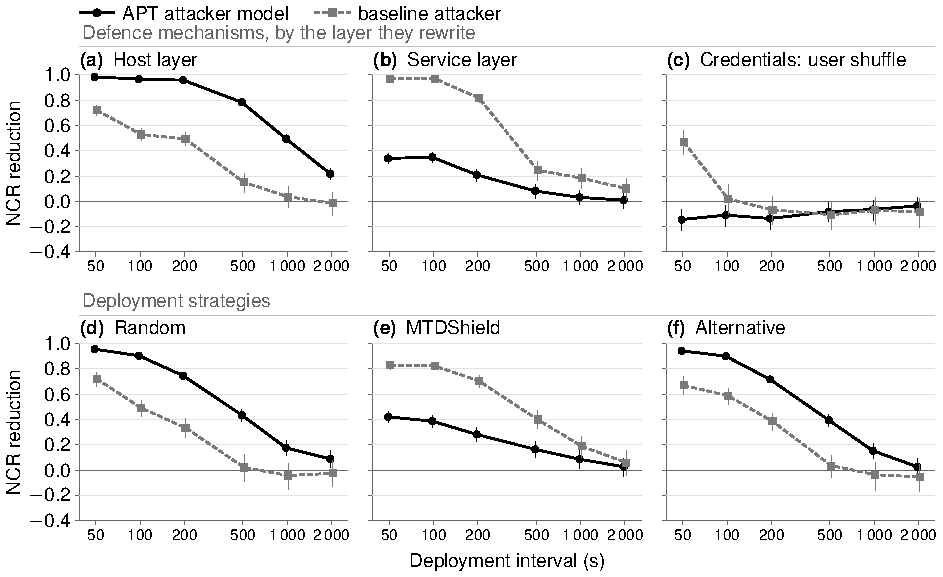
\includegraphics{fig_5-3-2b_interval_headline}
  % 2026-09-30 (Marc): the ASP reduction figure merged in as panels (g) to (l). Caption
  %  session-written from the two it replaces. DRAFT STATE --- ratify on read.
  % 2026-10-02 (results_presentation_standard.md P2): "1 with no whisker" was false at 1 000 seeds
  %  (random at 200 s, host topology shuffle at 500 s: one run in 4 000 each); the table separates them.
  % 2026-10-02 (Marc: "if somebody just read the captions ... they could figure out what's happening";
  %  results_presentation_standard.md S4, I1-I3, T2, F5): caption rewritten to read the float alone,
  %  decoding only; metrics stay defined in Section 4.5. Session-written, DRAFT STATE --- ratify on read.
  \caption[The same MTD measured against each attacker, across the deployment interval]{NCR reduction, panels~(a) to~(f), and ASP reduction, panels~(g) to~(l), (Section~\ref{sec:evaluation-metrics}) against the deployment interval, for the APT attacker model, its attack profiles $c_1$ to $c_4$ combined (solid, 4\,000 runs per point, 1\,000 per attack profile) and for the baseline attacker (dashed, 1\,000 runs per point). A reduction is 1 when no host is compromised (NCR) or no run compromises a target host (ASP), 0 when as many as with no MTD, and negative when more. For each reduction, the first row gives the MTD mechanisms by the layer each reconfigures (Table~\ref{tab:defence-mechanisms}), each deployed alone, a layer's line the mean over its mechanisms; the second row gives the deployment strategies: random, MTDShield (Appendix~\ref{app:mtdshield}) and alternative (Table~\ref{tab:deployment-strategies}). A point at 1 is a reduction of 1 or one above 0.99, which Table~\ref{tab:eff-interval-values-asp} tells apart. The interval axis is logarithmic; the NCR rows' y-axis starts at $-0.4$, the ASP rows' at $-1$. Whiskers: 95\,\% percentile bootstrap intervals over runs; where none shows, the interval is narrower than the marker. Tables~\ref{tab:eff-interval-values} and~\ref{tab:eff-interval-values-asp} give the values.}
  \label{fig:eff-cross-arm}
\end{figure}

% MOVED 2026-09-25 (handoff B9/F12): the headline's values table sits with the headline
%  figure, whose caption points to it; it was input at the end of §5.3.3.
% MOVED 2026-09-30 to Appendix F (Marc): its 200 s column repeated Table 5.5's; the body
%  keeps the ranking table, and the appendix carries the ASP reduction values beside it.

% REMOVED 2026-09-13 (stage-2 audit): fig:eff-delay. Survival curves are no
% corpus genre and ten conditions x two arms is twenty curves. Delay to first
% compromise is a column of tab:eff-conditions with censoring stated. IF Marc's
% horizon ruling (handoff §15) makes time to a compromise checkpoint the
% primary, the figure that replaces this is Zhang's form: a bar per condition of
% the time-to-checkpoint quantity, one series per attacker.

% REWORKED 2026-09-13 (stage-2 float audit, ch5 design handoff §18) --- kept as is (results table; the grade
% vocabulary lives at this definition site).
% POPULATED 2026-09-17 as a generated fragment (tools/ch5_effectiveness_figures.py;
% caption in the fragment). Ranks per arm at each interval; Spearman's rho
% with a seed-bootstrap interval and the family contrast (Cliff's delta,
% network against application layer) in the footnote, per the 2026-09-09
% inference ruling. DRAFT STATE --- ratify on read.
% REWORKED 2026-09-25 (Marc; register E7, applied to the two-interval corpus
% ahead of the E6 rank grid): the APT attacker model is the base --- its columns
% first, rows in its rank order; the footnote and its two statistics gone
% (Marc: "it's not fitting"); caption decode-only; type size as Table 5.4.
% Spearman's rho and the layer contrast (Cliff's delta) stay in numbers.json
% §s542 for the body, if the body wants them.
% REPLACED 2026-09-25 (results context §8j, Q10): the rank grid over the six
% deployment intervals (tools/ch5_sweep_figures.py --only ranks); a dash where the
% condition's interval includes zero. DRAFT STATE --- ratify on read.
% REPLACED 2026-09-25 (Marc on the draft: "the rankings ... what they mean to me";
% results context §8j-3): the values behind Figure 5.4, both attackers at every
% interval, rows grouped as its panels, grey where the interval includes zero
% (tools/ch5_sweep_figures.py --only values). The rank grid's fragment stays on
% disk. DRAFT STATE --- ratify on read.
% MOVED 2026-09-25 to §5.3.3 (Marc: "table 5.3 is currently encapsulating ... all the
% deployment intervals, which is not the focus of 5.3.2 ... the focus of 5.3.2 is
% literally the attacker model"; results context §8j-4). In its place, both
% attackers ranked at 200 s on every metric of Table 4.3, ranks by Scott-Knott ESD
% with ties shared (tools/ch5_sweep_figures.py --only ranking; the method is owed
% to §4.5, Marc drafting). DRAFT STATE --- ratify on read. PRELIMINARY: 100 seeds.
% --- P3: after Figure fig:eff-cross-arm, before % GENERATED by tools/ch5_sweep_figures.py from data/results/ch5_defended/numbers_reported.json
%   (section ranking; ranks by Scott-Knott ESD, data/results/ch5_defended/sk_esd.py). Do not hand-edit.
% 2026-09-25 (Marc: "we have to have some ranks ... ranking with ties"; results context §8j-4):
%   the two attackers side by side at one interval, all of Table 4.3's metrics. DRAFT STATE --- ratify on read.
% 2026-09-30: ranked on hosts compromised per seed (NCR reduction, the headline); ASP reduction
%   beside it (section 5.3.2 carries both); MTTC at a target host (ruling H1).
% 2026-09-30 (Marc): NCR and ASP dropped, each the reduction beside it restated against the no-MTD
%   row (Tables F.3 and F.4 keep them). At footnotesize it is still wider than the text, so scriptsize (conventions).
% 2026-10-02 (Marc; docs/workflows/results_presentation_standard.md P2, S1-S2, N1): a blank cell is
%   not applicable (the reference's rank and reductions), a dash an MTTC not reported, > 0.99 a
%   reduction short of 1.
\begin{table}[tp]
  \centering
% rho (NCR reduction, the two columns) at 200 s: $0.01$ [$-0.19$, $0.05$]
  \caption[The MTD mechanisms and deployment strategies ranked against each attacker]{The MTD mechanisms and deployment strategies ranked by NCR reduction against each attacker, at a deployment interval of 200\,s; the APT attacker model averaged over $c_1$ to $c_4$. Bold: rank~1. Tables~\ref{tab:full-movement} and~\ref{tab:full-baseline} give each value's confidence interval, ASP reduction and MTTC.}
  \label{tab:eff-cross-arm}
  \tablestyle\rowcolors{4}{black!5}{}
  \begin{tabular}{@{}P{4.3cm}>{\centering\arraybackslash}p{1.0cm}>{\centering\arraybackslash}p{2.4cm}>{\centering\arraybackslash}p{1.0cm}>{\centering\arraybackslash}p{2.4cm}@{}}
    \toprule
    & \multicolumn{2}{c}{APT attacker model} & \multicolumn{2}{c}{Baseline attacker} \\
    \cmidrule(lr){2-3}\cmidrule(lr){4-5}
    MTD & Rank & NCR reduction & Rank & NCR reduction \\
    \midrule
    IP shuffle & \textbf{1} & $0.96$ & 2 & $0.68$ \\
    host topology shuffle & \textbf{1} & $0.95$ & 3 & $0.38$ \\
    complete topology shuffle & \textbf{1} & $0.95$ & 3 & $0.42$ \\
    random & 2 & $0.75$ & 4 & $0.33$ \\
    alternative & 3 & $0.72$ & 3 & $0.38$ \\
    service diversity & 4 & $0.36$ & \textbf{1} & $0.92$ \\
    MTDShield & 5 & $0.28$ & 2 & $0.68$ \\
    port shuffle & 6 & $0.20$ & \textbf{1} & $0.91$ \\
    OS diversity & 7 & $0.07$ & 2 & $0.68$ \\
    user shuffle & 8 & $-0.10$ & 5 & $-0.05$ \\
    \bottomrule
  \end{tabular}
\end{table}

%     (tab:eff-cross-arm). If Marc swaps the two tables (handoff B9/F12) so that the 200 s
%     ranking moves to §5.3.3, P3's first two sentences move with it and the last
%     sentence closes P2. ---
% REWRITTEN 2026-09-26 on Marc's read ("very rhetorically inflated ... literally we
%  just need to describe what's happening"; his step-through of every float is
%  the content, checked against the tracked numbers). Plain description: what the
%  float shows, the numbers that carry it, the APT property the metric records
%  (Table 3.2 via Section 4.5), a by-construction reason only where Marc gave one.
%  The agent draft it replaces is in git history (commit e83f280c). DRAFT STATE.
% 2026-09-30 (Marc: "in 5.3.2 you could have ASP reduction and NCR reduction"):
% ASP reduction beside NCR reduction where the profiles are pooled (400 runs, 36
% successes with no MTD); per profile (5 to 13 successes) it does not resolve, so
% Section 5.3.3 stays on NCR reduction. Numbers: numbers.json sweep_asp. DRAFT STATE.
Figure~\ref{fig:eff-cross-arm}(g) to~(l) shows the same comparison on ASP reduction
(Equation~\ref{eq:asp-reduction}). Against the APT attacker model no run
compromises a target host up to 200\,s under each host-layer mechanism, and up
to 100\,s under the random and the alternative deployment strategies.
The service layer removes \prelim{0.51} to \prelim{0.79} of its ASP up to 200\,s,
more than the \prelim{0.21} to \prelim{0.35} of its NCR. Against the baseline
attacker the layers keep their order: \prelim{0.86} to \prelim{0.97} for the
service layer up to 200\,s, against \prelim{0.49} to \prelim{0.83} for the host
layer. At 500\,s the host layer's reduction against the baseline attacker is
\prelim{$-0.22$}: more of its runs compromise a target host than with no MTD.

% MERGED 2026-09-30 into fig:eff-cross-arm as panels (g) to (l) (Marc).

% 2026-09-30, second read (Marc: NCR reduction is the finer instrument; the ASP version
% 'is just a colourful mess'): the NCR text restored verbatim; its numbers re-checked,
% numbers.json sweep identical to the verified version (0 of 498 cells differ). DRAFT STATE.
Table~\ref{tab:eff-cross-arm} ranks the MTD mechanisms and deployment strategies at 200\,s. The three host-layer
mechanisms share rank 1 against the APT attacker model and take ranks 2 and 3
against the baseline attacker; service diversity and port shuffle share rank 1
against the baseline attacker and take ranks 4 and 6 against the APT attacker
model. The two attackers' rankings are unrelated: Spearman's $\rho$ between their
NCR reductions is \prelim{$-0.03$}, with a 95\,\% bootstrap interval over seeds of
\prelim{$-0.19$} to \prelim{0.05}.
% [CONNECTIVE-PROSE PASS 2026-09-26, ch5 U7 cut] Cut: the third statement
%  of 5.3.3's object (preamble roadmap; 5.3.3's first sentence), stating
%  nothing established. SESSION-GENERATED on Marc's 2026-09-26 go-ahead
%  (docs/workflows/connective_prose.md; audit
%  docs/implementation/connective_prose_audit.md); prior text in git.
%  RATIFIED 2026-09-26 (Marc: 'I accept all this').

% GENERATED by tools/ch5_sweep_figures.py from data/results/ch5_defended/numbers_reported.json
%   (section ranking; ranks by Scott-Knott ESD, data/results/ch5_defended/sk_esd.py). Do not hand-edit.
% 2026-09-25 (Marc: "we have to have some ranks ... ranking with ties"; results context §8j-4):
%   the two attackers side by side at one interval, all of Table 4.3's metrics. DRAFT STATE --- ratify on read.
% 2026-09-30: ranked on hosts compromised per seed (NCR reduction, the headline); ASP reduction
%   beside it (section 5.3.2 carries both); MTTC at a target host (ruling H1).
% 2026-09-30 (Marc): NCR and ASP dropped, each the reduction beside it restated against the no-MTD
%   row (Tables F.3 and F.4 keep them). At footnotesize it is still wider than the text, so scriptsize (conventions).
% 2026-10-02 (Marc; docs/workflows/results_presentation_standard.md P2, S1-S2, N1): a blank cell is
%   not applicable (the reference's rank and reductions), a dash an MTTC not reported, > 0.99 a
%   reduction short of 1.
\begin{table}[tp]
  \centering
% rho (NCR reduction, the two columns) at 200 s: $0.01$ [$-0.19$, $0.05$]
  \caption[The MTD mechanisms and deployment strategies ranked against each attacker]{The MTD mechanisms and deployment strategies ranked by NCR reduction against each attacker, at a deployment interval of 200\,s; the APT attacker model averaged over $c_1$ to $c_4$. Bold: rank~1. Tables~\ref{tab:full-movement} and~\ref{tab:full-baseline} give each value's confidence interval, ASP reduction and MTTC.}
  \label{tab:eff-cross-arm}
  \tablestyle\rowcolors{4}{black!5}{}
  \begin{tabular}{@{}P{4.3cm}>{\centering\arraybackslash}p{1.0cm}>{\centering\arraybackslash}p{2.4cm}>{\centering\arraybackslash}p{1.0cm}>{\centering\arraybackslash}p{2.4cm}@{}}
    \toprule
    & \multicolumn{2}{c}{APT attacker model} & \multicolumn{2}{c}{Baseline attacker} \\
    \cmidrule(lr){2-3}\cmidrule(lr){4-5}
    MTD & Rank & NCR reduction & Rank & NCR reduction \\
    \midrule
    IP shuffle & \textbf{1} & $0.96$ & 2 & $0.68$ \\
    host topology shuffle & \textbf{1} & $0.95$ & 3 & $0.38$ \\
    complete topology shuffle & \textbf{1} & $0.95$ & 3 & $0.42$ \\
    random & 2 & $0.75$ & 4 & $0.33$ \\
    alternative & 3 & $0.72$ & 3 & $0.38$ \\
    service diversity & 4 & $0.36$ & \textbf{1} & $0.92$ \\
    MTDShield & 5 & $0.28$ & 2 & $0.68$ \\
    port shuffle & 6 & $0.20$ & \textbf{1} & $0.91$ \\
    OS diversity & 7 & $0.07$ & 2 & $0.68$ \\
    user shuffle & 8 & $-0.10$ & 5 & $-0.05$ \\
    \bottomrule
  \end{tabular}
\end{table}


% ~1 unit. The defence conditions against the movement attacker: the
% seven single mechanisms and the three deployment schemes, per profile,
% against the no-defence origin. Report the no-defence condition as the
% ORIGIN of a relative-change plot, not as its own series (He's form;
% Tay normalises by it; Brown plots it as a bar).
% NOTE the condition set is not the published matrix's --- three of the
% seven singles entered the pool afterwards and have NEVER run against
% the movement attacker.
% FIGURES (1) + TABLE (1):
%  Fig. F  breadth suppression relative to no defence, grouped bars,
%          x = condition, series = profile. PURPOSE: which defences bite
%          this attacker, and whether the answer is profile-dependent.
%  Tab. B  the condition x metric table for the movement arm: suppression,
%          delay to first compromise, blocked fraction, with intervals.
% OWED HERE, 2026-09-20 (setup handoff §AL3, §AM P10): "the movement attacker" in
% tab:eff-conditions is the four profiles POOLED, 400 runs against the baseline's
% 100 (analyse.py:398); say so once at the head of this section.
% [CONNECTIVE-PROSE PASS 2026-09-26, DS 5.3.3 heading] Marc 2026-09-26:
%  'deployment strategies is very clear ... change everything to
%  deployment strategies' (registry row re-ruled). Overturns the
%  2026-09-20 heading ruling: MTDShield is in this subsection.
%  SESSION-GENERATED on Marc's 2026-09-26 go-ahead
%  (docs/workflows/connective_prose.md; audit
%  docs/implementation/connective_prose_audit.md); prior text in git.
%  RATIFIED 2026-09-26 (Marc: 'I accept all this').
\subsection{MTD mechanisms and deployment strategies}
\label{subsec:eff-under-defence}

% REWORKED 2026-09-13 (stage-2 float audit, ch5 design handoff §18) --- grouped bars with no defence as the
% origin (He; Tay normalises; Brown's "None" bar), split into two lettered
% panels so that every condition label stays legible (Brown's Figs 4-5 are
% the named anti-pattern); short domain names mapped in the generator.
% POPULATED 2026-09-17 (tools/ch5_effectiveness_figures.py from the defended corpus;
% read in docs/implementation/pipeline/ogasp/ch5_s54_effectiveness_findings.md).
% Four lettered panels, not two: the interval is a crossed factor (Table 5.2),
% so singles / schemes are shown at each. Whiskers are seeded bootstrap
% intervals on the ratio of cell means. Caption edited for the four panels.
% DRAFT STATE --- ratify on read.
% REWORKED 2026-09-22 (scrutinise-figure pass; results context §8h): caption
% decode-only (schemes as Table 2.5 has them, one per interval from the pool;
% the aggregate named as a fifth series; the estimator decoded), the
% "intention" sentence gone to the body slots, two-line tick names for the two
% topology shuffles, the formula key line dropped (Table 5.2 holds it).
% DRAFT STATE --- ratify on read.
% EXTENDED 2026-09-25 (Marc: MTDShield as another execution-scheme column in
% Figure 5.5 and Tables 5.3 and 5.4; handoff 2026-09-25_mtdshield_preliminary_run.md):
% panels (b) and (d) gain random over MTDShield's four and MTDShield, run as
% released (Appendix E). PRELIMINARY: 100 seeds, 200 s and 2 000 s only; the
% short name for the matched control is proposed, Marc rules (handoff Q7).
% REPLACED 2026-09-25 (Marc on Jin's second pass; results context §8j, Q11-Q12):
% the depth is one line panel per mechanism, NCR reduction against the six
% deployment intervals, profiles in the chapter's hues and the baseline attacker
% dashed; the schemes follow as their own figure. Caption decode-only. DRAFT
% STATE --- ratify on read. PRELIMINARY: 100 seeds.
% DRAFT STATE 2026-09-25 --- agent-drafted on Marc's request ("each of the agents will
%  do each of the prose elements"); slot plan: handoff 2026-09-25_ch5_setup_defence_and_prose_slots.md
%  Part C D5 (S33-a ... S33-g), content = results-context 8j-2 amended D1-D4. Ratify on read.
%  Replaces: nothing (the subsection has no body text today); pastes in two places,


\begin{figure}[tp]
  \centering
  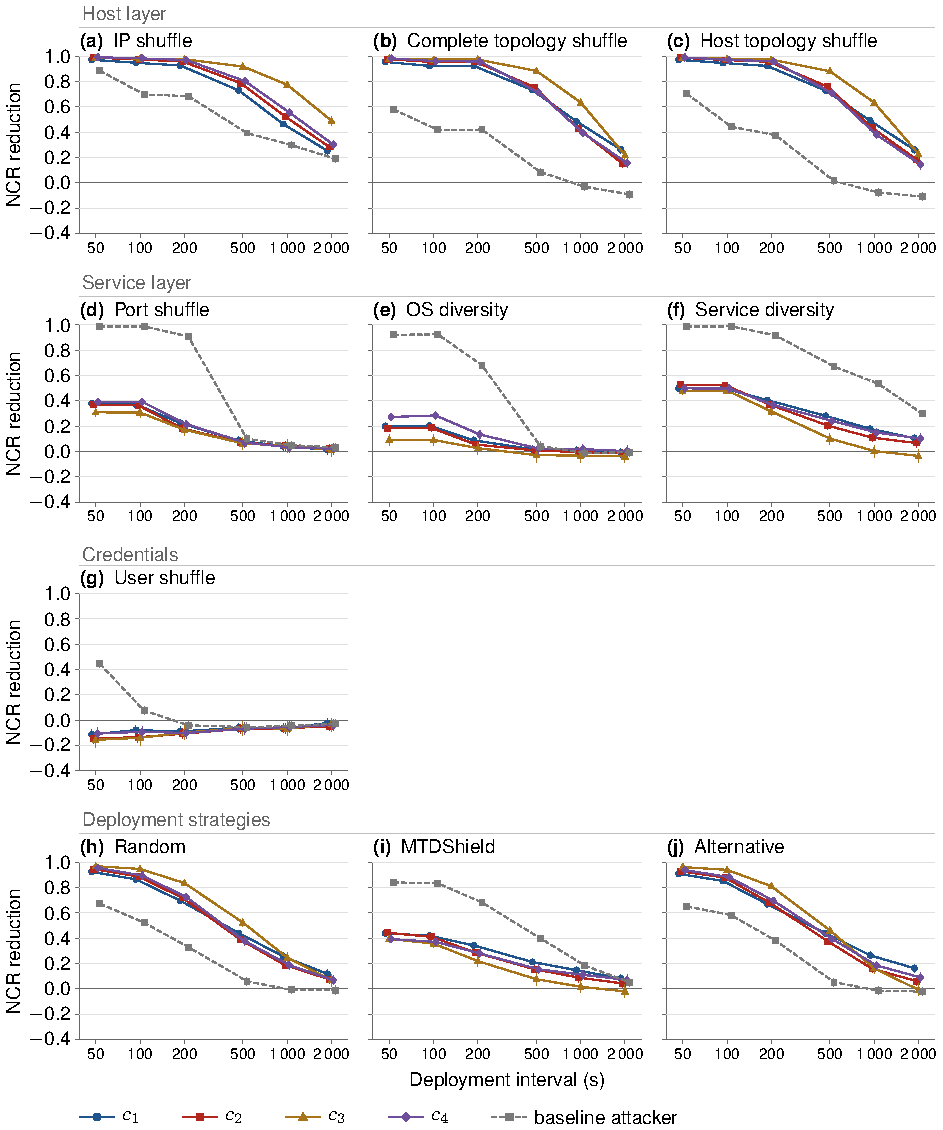
\includegraphics{fig_5-3-3b_interval_mechanisms}
  % 2026-09-30 (Marc): the deployment strategies' figure merged in as panels (h) to (j).
  %  Caption session-written from the two it replaces. DRAFT STATE --- ratify on read.
  % 2026-10-02 (Marc: "if somebody just read the captions ... they could figure out what's happening";
  %  results_presentation_standard.md S4, I1-I3, T2, F5): caption rewritten to read the float alone,
  %  decoding only; metrics stay defined in Section 4.5. Session-written, DRAFT STATE --- ratify on read.
  \caption[NCR reduction by MTD and attack profile, across the deployment interval]{NCR reduction (Section~\ref{sec:evaluation-metrics}) against the deployment interval for each attack profile $c_1$ to $c_4$ of the APT attacker model, with the baseline attacker dashed for comparison, 1\,000 runs per point: each MTD mechanism deployed alone, panels~(a) to~(g), in rows by the layer it reconfigures (Table~\ref{tab:defence-mechanisms}), and each deployment strategy, panels~(h) to~(j): random, MTDShield (Appendix~\ref{app:mtdshield}) and alternative (Table~\ref{tab:deployment-strategies}). NCR reduction is 1 when no host is compromised, 0 when as many as with no MTD, and negative when more. Table~\ref{tab:eff-interval-values} gives the baseline attacker's values, and the APT attacker model's with $c_1$ to $c_4$ combined. The interval axis is logarithmic. Whiskers: 95\,\% percentile bootstrap intervals over runs; where none shows, the interval is narrower than the marker.}
  \label{fig:eff-suppression-profiles}
\end{figure}

% NEW 2026-09-25 (results context §8j, Q12): the depth's second figure, the four
% execution schemes in the same form (tools/ch5_sweep_figures.py --only schemes).
% DRAFT STATE --- ratify on read. PRELIMINARY: 100 seeds.
% 2026-09-25: one row of three, random over MTDShield's four dropped (Marc).
%  marked PARAGRAPH 1 and PARAGRAPH 2 below.
%  Slots -> sentences:
%    P1 s1 = S33-a (D1, the part that holds at every interval: host three one effect
%            to 200 s against the model; IP shuffle apart from both topology shuffles
%            against the baseline attacker at every interval) + float pointer
%    P1 s2-s3 = S33-b (D3; carries D1's "part from 500 s" too, so it is said once)
%    P1 s4 = S33-c (D2, the exception, marked and not explained)
%    P2 s1 = S33-d (D4) + float pointer
%    P2 s2 = S33-d (the by-construction sentence: one per interval, three of seven host-layer)
%    P2 s3 = S33-f (the exponential timing distribution; \owed, see its second argument)
%    S33-e DROPPED: Appendix C states hosts reached, not the range of the 200 s reduction
%          (candidate wording kept as a comment at the foot, not live)
%    S33-g not drafted (conditional on A15; the simultaneous execution scheme is not run)
%    No chapter summary; no pointer to chapter 6 (the chapter ends on the last result).
%  Numbers (100 seeds; every one wrapped \prelim):
%    0.33  <- data/results/ch5_defended/numbers.json: sweep.by_interval["2000"].attacker.movement.ip_shuffle.point (0.33);
%             "half that" <- same path, complete_topology 0.16, host_topology 0.17 (ratio 0.48, 0.52: RE-CHECK at 1 000 seeds)
%             also printed in tab_5-3-2c_attacker_values.tex, IP shuffle row, APT 2 000 s
%    port shuffle whiskers include zero from 500 s <- sweep.by_interval["500"|"1000"|"2000"].attacker.baseline.port_shuffle lo < 0
%    service diversity keeps an effect to 2 000 s <- sweep.by_interval["2000"].attacker.baseline.service_diversity [0.22, 0.37]
%    0.12  <- sweep.by_interval["100"].attacker.movement: service_diversity.point - mtdshield.point = 0.120 (the largest of the six gaps)
%    0.90  <- sweep.by_interval["200"].attacker.baseline.port_shuffle.point (also tab_5-3-2c, 200 s)
%    0.14  <- regime.rank_block.suppression.baseline.port_shuffle.point (0.136) [in no float]
%    order unchanged (APT) <- regime.rank_block.ranks.movement against sweep.by_interval["200"].ranks.movement restricted to the nine
%    no sign change <- regime.rank_block.suppression.{movement,baseline}.*.point against sweep 200 s points

% ---- PARAGRAPH 1: directly under \label{subsec:eff-under-defence}, before Figure fig:eff-suppression-profiles ----
% REWRITTEN 2026-09-26 on Marc's read ("very rhetorically inflated ... literally we
%  just need to describe what's happening"; his step-through of every float is
%  the content, checked against the tracked numbers). Plain description: what the
%  float shows, the numbers that carry it, the APT property the metric records
%  (Table 3.2 via Section 4.5), a by-construction reason only where Marc gave one.
%  The agent draft it replaces is in git history (commit e83f280c). DRAFT STATE.
% 2026-09-30, second read (Marc: NCR reduction is the finer instrument; the ASP version
% 'is just a colourful mess'): the NCR text restored verbatim; its numbers re-checked,
% numbers.json sweep identical to the verified version (0 of 498 cells differ). DRAFT STATE.
Figure~\ref{fig:eff-suppression-profiles} shows each mechanism separately, for
each attack profile. On the host layer, all three mechanisms remove nearly all of
the APT attacker model's NCR up to 200\,s and less at longer intervals, IP shuffle
keeping the most (\prelim{0.33} at 2\,000\,s against \prelim{0.16} and
\prelim{0.17}); against the baseline attacker, IP shuffle gives more reduction
than either topology shuffle at every interval. On the service layer, service
diversity is the one mechanism that keeps a reduction against the baseline
% [CONNECTIVE-PROSE PASS 2026-09-26, S8 service layer] 'matches' named no
%  test; the declared one is a shared Scott-Knott rank (numbers.json
%  ranking.by_interval, baseline sk_esd: port shuffle rank 1 to 200 s, OS
%  diversity rank 1 to 100 s). Marc 2026-09-26: 'sure'. SESSION-GENERATED
%  on Marc's 2026-09-26 go-ahead (docs/workflows/connective_prose.md;
%  audit docs/implementation/connective_prose_audit.md); prior text in
%  git. RATIFIED 2026-09-26 (Marc: 'I accept all this').
attacker at every interval (\prelim{0.30} at 2\,000\,s). Port shuffle is not told apart from it up to 200\,s, since the two share a Scott--Knott rank there; OS diversity is told apart from it at every interval. Port shuffle is told apart from zero up to 1\,000\,s, OS diversity up to 500\,s.
% [CONNECTIVE-PROSE PASS 2026-09-26, S8 profiles] 'move together' /
%  'separates' named no test; replaced by the values (numbers.json
%  sweep.by_interval[500].profile; c3 lower bounds 0.82-0.87 against the
%  others' upper 0.76-0.86). The universal 'move together under every
%  mechanism' is dropped: it had no test behind it. SESSION-GENERATED on
%  Marc's 2026-09-26 go-ahead (docs/workflows/connective_prose.md; audit
%  docs/implementation/connective_prose_audit.md); prior text in git.
%  RATIFIED 2026-09-26 (Marc: 'I accept all this').
User shuffle reduces neither attacker's NCR from 200\,s. At 500\,s each host-layer mechanism keeps a larger reduction against $c_3$ than against the other attack profiles, \prelim{0.86} to \prelim{0.91} against \prelim{0.71} to \prelim{0.82}, and the intervals do not overlap.

% ---- PARAGRAPH 2: between Figure fig:eff-suppression-profiles and Figure fig:eff-schemes-profiles ----
% REWRITTEN 2026-09-26 on Marc's read ("very rhetorically inflated ... literally we
%  just need to describe what's happening"; his step-through of every float is
%  the content, checked against the tracked numbers). Plain description: what the
%  float shows, the numbers that carry it, the APT property the metric records
%  (Table 3.2 via Section 4.5), a by-construction reason only where Marc gave one.
%  The agent draft it replaces is in git history (commit e83f280c). DRAFT STATE.
% [CONNECTIVE-PROSE PASS 2026-09-26, S24 c_agg] c_agg was drawn in Figures
%  5.5 and 5.6 and promised by the 5.3 preamble but read nowhere (Marc
%  2026-09-26: 'that's an issue'). Values from numbers.json
%  sweep.by_interval[200].profile; user shuffle is the one mechanism where
%  c_agg (-0.11) sits above c1-c4 (-0.16 to -0.12). DRAFT plain
%  description, numbers checked. SESSION-GENERATED on Marc's 2026-09-26
%  go-ahead (docs/workflows/connective_prose.md; audit
%  docs/implementation/connective_prose_audit.md); prior text in git.
%  RATIFIED 2026-09-26 (Marc: 'I accept all this').
% 2026-09-30, second read (Marc: NCR reduction is the finer instrument; the ASP version
% 'is just a colourful mess'): the NCR text restored verbatim; its numbers re-checked,
% numbers.json sweep identical to the verified version (0 of 498 cells differ). DRAFT STATE.
% 2026-09-30, scrutiny round: the c_agg sentence cut (0.69 was 0.67; c_agg lay
% outside the range under service diversity; gaps of 0.01 inside the noise); the
% deployment strategies' split, which the figure shows, in its place. DRAFT STATE.
% 2026-09-30: float reference only, to the merged figure's panels.
Figure~\ref{fig:eff-suppression-profiles}(h) to~(j) shows the deployment strategies, for each
attack profile. Under MTDShield the baseline attacker's NCR reduction lies above
every attack profile's up to 1\,000\,s; under the random deployment strategy it
lies below every profile's at every interval, and under the alternative
deployment strategy up to 1\,000\,s. Against the APT attacker model, averaged over $c_1$ to $c_4$
(Table~\ref{tab:eff-interval-values}), MTDShield stays within
% [CONNECTIVE-PROSE PASS 2026-09-26, S7 MTDShield mechanism] Mechanism
%  removed from the results (Marc 2026-09-26: 'that's my bet'). PARKED FOR
%  CHAPTER 6: Marc's reading is that MTDShield tracks service diversity
%  because it chooses service diversity at 70 to 76 % of its decisions
%  (Appendix E.5) --- an interpretation, for the discussion.
%  SESSION-GENERATED on Marc's 2026-09-26 go-ahead
%  (docs/workflows/connective_prose.md; audit
%  docs/implementation/connective_prose_audit.md); prior text in git.
%  RATIFIED 2026-09-26 (Marc: 'I accept all this').
\prelim{0.12} of service diversity at every interval.
\owed{Replacing the near-periodic timing distribution with the exponential one
at 200\,s changes the sign of no reduction for either attacker, and the APT
% [CONNECTIVE-PROSE PASS 2026-09-26, DS 5.3.3 owed] Marc 2026-09-26:
%  'deployment strategies is very clear ... change everything to
%  deployment strategies' (registry row re-ruled). SESSION-GENERATED on
%  Marc's 2026-09-26 go-ahead (docs/workflows/connective_prose.md; audit
%  docs/implementation/connective_prose_audit.md); prior text in git.
%  RATIFIED 2026-09-26 (Marc: 'I accept all this').
attacker model keeps its order of the seven mechanisms and two deployment strategies; against the baseline attacker service diversity stays first, but port
shuffle falls from \prelim{0.90} to \prelim{0.14}, below IP shuffle.}{Section
5.3.3: the exponential timing distribution's values sit in no float, so an
appendix table is owed (200 s, both attackers, the seven MTD mechanisms and two deployment strategies, with
intervals); MTDShield was not run under it; the interrupt-tally sanity flag
raised in the regime runs is not yet investigated}
% ---- S33-e, DROPPED (not live). Candidate for Marc's ruling, if the analyser emits the
%  reduction range with its interval (Appendix C tabulates hosts reached only;
%  from tab_C-1a's cells the random execution scheme's reduction at 200 s is
%  1 - 7.5/13.4 = 0.44, 1 - 2.1/8.1 = 0.74, 1 - 0.3/3.0 = 0.90 across the
%  low-and-slow band; derived here, stated nowhere):
%  "The size of the random execution scheme's reduction at 200\,s depends on the
%   declared low-and-slow dwell time, from \prelim{0.44} to \prelim{0.90} across
%   that family's band (Appendix~\ref{app:dwell-robustness})."

% MERGED 2026-09-30 into fig:eff-suppression-profiles as panels (h) to (j) (Marc).

% REWORKED 2026-09-13 (stage-2 float audit, ch5 design handoff §18) --- kept despite its cut mark: intervals cannot
% be read off bars and He's TABLE III is the precedent. Gains the DELAY TO
% FIRST COMPROMISE column with censoring stated, which is where the delay
% channel now lives (fig:eff-delay removed: survival curves are no corpus
% genre and twenty of them would not read). Adjacent conditions whose
% intervals overlap carry a footnote mark rather than a rank.
% POPULATED 2026-09-17 as a generated fragment (tools/ch5_effectiveness_figures.py;
% caption in the fragment). Rows are the nine conditions at each interval,
% ordered by suppression, the model pooled over its four profiles, the
% no-defence reference once; the censored share of the delay column is the
% share of runs denied every host (one column, not two); overlapping
% neighbours carry the dagger. DRAFT STATE --- ratify on read.
% REWORKED 2026-09-25 (Marc accepted 1 and 2): columns in Table 4.3's order
% under its two class headers, attack outcome (ASP, NCR, MTTC) then MTD
% effectiveness (NCR reduction, attack actions blocked); the no-host-compromised
% column, which is no metric, is folded into the MTTC cell as the share of runs
% MTTC is taken over. Rows still ordered by NCR reduction.
% RETIRED 2026-09-25 (results context §8j-4): superseded by Table 5.3's ranking at
% 200 s (both attackers, every metric) and by the appendix's two tables, which carry
% this table's intervals for each attacker. Fragment stays on disk.
% MOVED HERE 2026-09-25 from §5.3.2: the NCR reduction per defence, attacker and
% deployment interval, the backing for the interval sweep. DRAFT STATE.

% RETIRED 2026-09-23 (Marc's rulings R3, R4; handoff
% 2026-09-22_ch5_two_phase_restructure.md §6, in git history): the subsection "Comparison with
% prior evaluations" (subsec:eff-lineage, tab:eff-lineage) --- subsumed into the
% phase-two floats, the lineage's configurations run and MTDShield a scheme column
% (E6) --- and the section "Defence efficiency" (sec:efficiency, fig:eff-frontier,
% fig:eff-cost-decomposition, tab:eff-cost; Marc: "defence efficiency just goes").
% The comment blocks and floats are in git history at the parent of this commit;
% the generated fragments stay on disk, struck through in FLOATS.md.
% =====================================================================
\section{Ablation studies}
\label{sec:ablation}

% RESTRUCTURED 2026-09-28 (Marc: "5.4 structure I accept"): one section, a
% subsection per ablated component, named as in chapter 4 (4.4.4 -> 5.4.1,
% 4.4.5 -> 5.4.2); Tay's "6.5 Ablation Studies" the local precedent. The shared
% design (c1 to c4; no defence, IP shuffle and OS diversity at 200 s and
% 2 000 s; the same seeds; the threshold, folded here from 4.5.4) is declared once here and
% not repeated below. Handoff 2026-09-28_vulnerability_memory_on.md, Part B.
% FOLDED FROM 4.5.4, 2026-09-30: the ablation threshold is declared here,
%  where ablations are first used (evaluation_conventions.md §a). DRAFT STATE.
% 2026-09-30 (Marc: "how do you define negligible ... I don't really
%  understand what [Cohen's d] is"; "a shared definition ... in 5.4 because it
%  serves both ablations"): d defined in one clause, in words; its interval
%  stated over seeds, as ablation.py and memory_ablation.py compute it (the
%  per-seed mean over c1 to c4, the pooled SD of the two arms' per-seed
%  means). Cohen names 0.2 a small effect; "negligible" below it is the
%  convention built on that, so the sentence says so and does not put the
%  word in Cohen's mouth. DRAFT STATE --- ratify on read.
% 2026-10-02 SESSION-DRAFTED from Marc's selection rule ("reversible steps in
%  our method ... high risk to validity ... contributed to a property we were
%  marking"; the dwell times "cannot be removed"), replacing the preamble
%  placeholder. DRAFT STATE, ratify on read.
Three steps of the method can be removed with the APT attacker model still
running: the partition into attack profiles, the failure matrix and the
vulnerability memory. Each is our judgement, and so a risk to the validity of
this chapter's results, and each gives the model one property of an APT
attacker (Table~\ref{tab:attacker-properties}): objective conditioning,
adaptivity and learning. The other parts of the model, such as the tactic
durations, cannot be removed, and Appendix~\ref{app:sensitivity} varies
their values instead.

Each ablation compares the APT attacker model with and without one component,
on the same seeds. The difference is measured by Cohen's $d$: the difference
between the two means divided by their standard deviation over seeds, reported
with its 95\,\% bootstrap interval over seeds. A difference is negligible when
$d$ is below 0.2, the value Cohen \citep{cohen1988statistical} calls a small effect:
the component then moves the result by less than a fifth of its ordinary
variation from one seed to the next.
% 2026-10-01 (Marc: "one table 5.6 covering both ablations in one form"; "the
%  main headline figure of 5.4 [is] the table and both of the subsections talk
%  about it"): SESSION-GENERATED sentence introducing it. DRAFT STATE.
Table~\ref{tab:ablation} gives the three ablations with 20 services per
operating system, the network of every other result in this chapter.

% GENERATED by data/results/ch5_defended/ablation_table.py from ablation_numbers.json and
% memory_ablation_numbers.json; never hand-edit. Section 5.4's headline float, cited by both subsections.
% Caption DRAFT STATE 2026-10-01, ratify on read.
\begin{table}[tp]
  \centering
  \caption[The APT attacker model with and without each ablated component]{The APT attacker model with and without each ablated component, averaged over $c_1$ to $c_4$, on the same 1\,000 seeds, with 20 services per operating system: NCR, Cohen's $d$ on NCR, with minus without, with its 95\,\% bootstrap interval over seeds, and NCR reduction (Section~\ref{sec:evaluation-metrics}).}
  \label{tab:ablation}
  \tablestyle\rowcolors{1}{}{}
  \begin{tabular}{@{}lccccc@{}}
    \toprule
    & \multicolumn{3}{c}{NCR} & \multicolumn{2}{c}{NCR reduction} \\
    \cmidrule(lr){2-4}\cmidrule(lr){5-6}
    MTD & with & without & Cohen's $d$ & with & without \\
    \midrule
    \multicolumn{6}{@{}l}{\emph{Failure matrix}} \\
    no MTD & 0.169 & 0.165 & $+0.06$ [$+0.02$, $+0.09$] & --- & --- \\
    IP shuffle, 200\,s & 0.007 & 0.006 & $+0.13$ [$+0.06$, $+0.20$] & 0.96 & 0.96 \\
    IP shuffle, 2\,000\,s & 0.112 & 0.108 & $+0.10$ [$+0.05$, $+0.15$] & 0.33 & 0.35 \\
    OS diversity, 200\,s & 0.156 & 0.157 & $-0.01$ [$-0.05$, $+0.03$] & 0.07 & 0.05 \\
    OS diversity, 2\,000\,s & 0.170 & 0.168 & $+0.04$ [0.00, $+0.08$] & $-0.01$ & $-0.02$ \\
    \addlinespace
    \multicolumn{6}{@{}l}{\emph{Vulnerability memory}} \\
    no MTD & 0.167 & 0.163 & $+0.08$ [$+0.01$, $+0.16$] & --- & --- \\
    service diversity, 200\,s & 0.106 & 0.104 & $+0.05$ [$+0.01$, $+0.11$] & 0.36 & 0.36 \\
    OS diversity, 200\,s & 0.156 & 0.151 & $+0.08$ [$+0.01$, $+0.17$] & 0.07 & 0.07 \\
    \bottomrule
  \end{tabular}
\end{table}



\subsection{Attack profiles by objective}
\label{subsec:ablation-attack-profiles}

% [NEW 2026-10-02: the third ablation, first in chapter 4's order (Section 4.2
%  before 4.4.4 and 4.4.5). Marc: "we're just winding back a step, so there
%  will be overlap". Design and the six moves: handoff
%  2026-10-02_c_agg_ablation_proposal.md. No new runs: the attack graph ran in
%  every cell of the reported corpus. Numbers: partition_ablation.py ->
%  partition_ablation_numbers.json (n = 100 and 1 000). "with" = c1-c4 averaged
%  with equal weight, as the chapter pools; "without" = the attack graph.
%  PRELIMINARY READ, 1 000 seeds (d with minus without):
%    no MTD NCR 0.171 vs 0.189, d -0.28 [-0.35, -0.22]
%    IP shuffle 200 s 0.007 vs 0.013, d -0.47; NCR reduction 0.96 vs 0.93
%    IP shuffle 2 000 s 0.114 vs 0.145, d -0.56; NCR reduction 0.33 vs 0.24
%    OS diversity 200 s d -0.26; 2 000 s d -0.21; NCR reduction within 0.03
%    |d| >= 0.2 in 48 of 61 cells of the grid; largest IP shuffle 1 000 s, -0.76
%    distinct attack paths, 1 000 runs each, k = 5: 254 with, 535 without
%  Not negligible: the pre-declared size-matched control (proposal R5) decides
%  objective against corpus size. Placeholders only; Marc dictates.]
% 2026-10-02 DRAFT STATE, SESSION-DRAFTED on Marc's ask ("draft attack
%  profile by objective ... use some of my language ... my thinking and
%  logic ... don't go too deep into the nuance"), in the moves of 5.4.2 and
%  5.4.3: purpose (his: different objectives warrant different behaviour;
%  the profiles captured it; does it change the outcome of MTD evaluation?),
%  variant, prediction, manipulation check, outcome, scope. His expectation
%  (outcomes similar, because the profiles drive the simulator's existing
%  attack actions) is chapter 6's, with the why. Numbers:
%  partition_ablation_numbers.json, n = 1 000: distinct attack paths over the
%  first five steps, 1 000 runs each (with: one profile per seed in turn);
%  the grid has 61 settings (no MTD; ten MTD conditions x six intervals), d
%  negative in all 61, the interval wholly beyond 0.2 in 30, inside in 7,
%  crossing in 24. Weight-carrying flows: 14, 6, 5, 4 of 29 (Section 4.3's
%  operator rule). The control's result is owed (run_partition_control.sh).
%  RATIFY ON READ.
The attack profiles rest on APT attackers with different objectives behaving
differently (Section~\ref{sec:attack-profiles}), and $c_1$ to $c_4$ do
behave differently: they open their campaigns along different attack paths
(Figure~\ref{fig:aio-coverage}(b)). The partition into attack profiles is our
judgement, so this section tests whether it also changes any result of this
chapter. Without the partition, the APT attacker model runs on the attack
graph itself (Section~\ref{sec:technique-graph}), built by the same
construction from every attack flow, so at each tactic it may follow the attack flows
of any objective. If the partition matters, the attacker without it should
take more distinct attack paths, and MTD should remove a different share of
what it compromises. The attack graph ran beside $c_1$ to $c_4$ on the same
1\,000 seeds, with no MTD and under every MTD mechanism and deployment
strategy at every deployment interval (Table~\ref{tab:experiment}).

Removing the partition changes where the attacker goes. Over its first five
steps, the attacker without the partition takes 535 distinct attack paths in
1\,000 runs; with it, taking each attack profile in turn, 254.

Removing the partition also changes what the attacker achieves
(Table~\ref{tab:ablation}). With no MTD, the attacker without it compromises
more of the network: NCR is 0.189 against 0.171, and $d$ is $-0.28$. The
difference carries into MTD effectiveness. Under IP shuffle at 2\,000\,s, NCR
reduction is 0.24 without the partition and 0.33 with it; under OS diversity
the two differ by at most 0.03. Across all 61 settings of MTD mechanism,
deployment strategy and interval, the attacker without the partition
compromises more in every one, and the interval of $d$ lies wholly beyond the
negligible band in 30 of them (Table~\ref{tab:ablation-attack-profiles}).

The partition does two things at once: it sorts the attack flows by
objective, and it builds each Petri net from fewer of them, 4 to 14 of the 29
that carry weight against all 29 for the attack graph. A net built from fewer
attack flows offers fewer attack paths, whatever their objective. To separate the
two, ten random partitions of the attack flows, each group the same size as
an attack profile, were built and run in the same way.

% [2026-10-03 DRAFT STATE, SESSION-DRAFTED: the control's result and the
%  verdict, filling the two placeholders. RATIFY ON READ. Numbers:
%  partition_control.py -> partition_control_numbers.json, n = 1 000 seeds,
%  10 partitions, 74 500 + earlier runs, 0 errors. NCR (agg / real / random
%  mean): none 0.189 / 0.171 / 0.121; IPS 200 0.013 / 0.007 / 0.007; IPS 2000
%  0.145 / 0.114 / 0.078; OSD 200 0.174 / 0.159 / 0.113; OSD 2000 0.187 /
%  0.174 / 0.121. Real above all ten random partitions in 4 of 5 settings
%  (d real vs random +0.16 to +2.32 there); IPS 200 s at the floor, real 5th
%  of 11. NCR reduction (agg / real / random mean [range]): IPS 200 0.93 /
%  0.96 / 0.94 [0.88, 0.97]; IPS 2000 0.24 / 0.33 / 0.35 [0.20, 0.44]; OSD
%  200 0.08 / 0.07 / 0.06 [0.04, 0.10]; OSD 2000 0.01 / -0.02 / -0.00
%  [-0.02, 0.01]. Real-vs-random d and reductions from a scratch read of the
%  same runs (pc_extra.py), not yet in the numbers file.]
The random partitions compromise less than either. With no MTD, their NCR is
0.121 on average over the ten, against 0.171 with the attack profiles and
0.189 without the partition. The attack profiles compromise more than every
random partition in four of the five settings of Table~\ref{tab:ablation};
in the fifth, IP shuffle at 200\,s, NCR is below 0.015 in every arm. NCR
reduction with the attack profiles lies among the random partitions'. Under
IP shuffle at 2\,000\,s it is 0.35 on average over the random partitions
(0.20 to 0.44), against 0.33 with the attack profiles and 0.24 without the
partition; under OS diversity the three differ by at most 0.03.

The ablation covers every MTD mechanism, deployment strategy and interval of
this chapter. Removing the partition raises what the attacker compromises,
by a small to medium effect. Sorting the attack flows by objective keeps
more of that compromise than a partition of the same sizes. The change in
NCR reduction is what any partition of these sizes produces.
Chapter~\ref{ch:discussion} discusses why.

\subsection{Failure matrix}
\label{subsec:ablation-failure-matrix}

% [NEW 2026-09-26, supervisor screen plan item 6 (Marc: "we tried it and it
%  didn't work, here's the ablation study"; "present the ablation study in a
%  very clear manner"). Plain description of the float, per conventions §j2 as
%  amended 2026-09-26; the interpretation, why the failure matrix changes
%  little, is chapter 6's. Numbers: data/results/ch5_defended/ablation_numbers.json
%  (100 seeds, every one \prelim); table generated by ablation.py. The verdict
%  uses Section 4.5.4's threshold only. Scope as run: run_corpus.py group
%  "blind". DRAFT STATE, ratify on read.]
% [RESHAPED 2026-09-28 (Marc, chat: "I don't doubt the validity of the data but
%  I'm doubting the narrative"): prediction, manipulation check, outcome, with
%  fig:ablation. The so-what is Marc's: the failure matrix "changes where the
%  attacker goes but doesn't change what it achieves". Plain description; why
%  is chapter 6's. Numbers: ablation_numbers.json at 1 000 seeds (seeds 0-99
%  from the corpus, 100-999 from runs_ablation.jsonl, the same code; seeds 0
%  and 3 re-ran bit-identical). The verdict is the point reading Section 4.5.4
%  declares; every interval also lies inside +-0.2, the IP shuffle 200 s one
%  only just (upper end 0.1999 of a 2 000-resample percentile), so the prose
%  says it reaches the edge of the band. RULING owed on point vs interval
%  reading (recommended: the interval, declared in 4.5.4). Context critic
%  re-review 2026-09-28: every number checked against the JSON and raw runs.
%  DRAFT STATE, ratify on read.]
Every value of the failure matrix is our judgement
(Section~\ref{subsec:failure-matrix}), so this section tests whether any result
of this chapter depends on it. Without the failure matrix, a failure routes as a
success does. If the failure matrix matters, the attacker without it should move
on after a failure as though it had succeeded, and compromise more of the
network. The APT attacker model was run on $c_1$ to $c_4$ with the failure
matrix and with every factor of it set to one, on the same 1\,000 seeds, with no
MTD and under IP shuffle and OS diversity at the 200\,s and 2\,000\,s
deployment intervals (Table~\ref{tab:experiment}).

% 2026-10-01, THE §5.4 FLOAT SCRUTINY on Marc's rulings (record: handoff
%  2026-09-28_vulnerability_memory_on.md, "§5.4 float scrutiny"): Figure 5.7
%  CUT ((b) printed Table 5.6's d column; (a)'s headline share is the declared
%  weight read back, told here in one sentence). DELETIONS ONLY in Marc's prose,
%  no rewording: the numbers that now sit in no float (the next-action shares,
%  the c2 shares, "at most 0.21", the per-profile hosts, time lost, the NCR
%  pair Table 5.6 prints); "at most 0.020" -> "0.02" at the table's precision;
%  "execution schemes" -> "deployment strategies" (registry). The six-sentence
%  slots for Marc's dictation are in the handoff. DRAFT STATE.
% OWED: this ablation ran with the vulnerability memory off (the corpus core
%  arm at seeds 0-99 is bit-identical to the memory ablation's off arm); rerun
%  both arms with the memory on at 1 000 seeds (Marc 2026-10-01: "we can rerun
%  that when we do the ablation to 1 000 seeds"). Until then Table 5.6's two
%  no-MTD "with" rows differ (0.169 against 0.167).
Removing the failure matrix changes where the attacker goes after a failure.
After a failed initial access, the model with the
failure matrix goes back to reconnaissance in 0.76 to 0.83 of cases on $c_1$,
$c_3$ and $c_4$ (on $c_1$, the weight of 0.750 that Figure~\ref{fig:gspn-gadget}
draws), and the model without it in 0.08 to 0.10.
On $c_2$ the model goes back to reconnaissance after
no failed initial access, with or without the failure matrix.

% 2026-10-02: the owed rerun is done (both arms with the vulnerability memory
%  on, 1 000 seeds, ablation_numbers_memory.json; the with arm equals the
%  partition block's). Numbers updated, owed mark closed; the IP shuffle 200 s
%  interval is now [+0.057, +0.193], inside the band, so the edge clause goes.
%  SESSION-EDITED, DRAFT STATE.
Removing the failure matrix does not change what the attacker achieves
(Table~\ref{tab:ablation}). With no MTD and under IP shuffle and OS diversity
at both intervals, $d$ is below 0.2 and every interval lies inside the
negligible band. The largest is 0.13, under IP shuffle at 200\,s. In four of the five cells the model with the
failure matrix compromises more, the opposite direction to the prediction.
The NCR reduction of each MTD mechanism differs by at most 0.02 between the two
models.

The ablation covers two of the seven MTD mechanisms, both deployment
intervals and $c_1$ to $c_4$; the other mechanisms and the deployment strategies were not run without the
failure matrix. Within that scope,
the results of this chapter do not depend on the failure matrix.
Chapter~\ref{ch:discussion} discusses why.

\subsection{Vulnerability memory}
\label{subsec:ablation-vulnerability-memory}

% [NEW 2026-09-28: the second ablation (Marc's ruling; handoff
%  2026-09-28_vulnerability_memory_on.md). Heading ruled 2026-09-28. Pre-check at 20 seeds, no
%  defence, §11.11 of the ch6 board: the memory operates (22--39 types
%  re-exploited per run) and moves no hosts; a perfect exploit adds about
%  none; the OS check refuses about half of all exploit attempts, and removing
%  it adds about two hosts. Report whatever the 1 000 seeds show.]
% [DRAFT STATE 2026-09-30 --- assembled by the session on Marc's ask ("put in
%  the hard work, assemble the ablation subsection ... and propose it to me"),
%  from his walk of the six moves in chat: purpose ("does the vulnerability
%  memory as implemented actually change the attack outcome, and does this
%  change when we constrain the diversity pool"), variant (on and off, the pool
%  constrained), prediction ("smaller service pools will result in the attacker
%  performing more successful exploits"), float (pool on the x-axis, two
%  lines), his reading ("the mechanism works but the outcome doesn't change";
%  "the hypothesis is ... only half right"; "the chapter's results do not
%  depend on the memory"). Same moves and closer as 5.4.1. The why (a host
%  needs two exploit visits; the failure verdict routes the token away and a
%  later port scan reveals the next hop) is Chapter 6's, as 5.4.1's is: ch5
%  describes, ch6 explains. Numbers: memory_ablation_numbers.json, 100 seeds,
%  every one \prelim; the 1 000-seed swap is owed. Table generated by
%  memory_ablation.py. The figure is a placeholder until it is drawn (Marc:
%  figures after the draft). RATIFY ON READ.
%  SCRUTINY 2026-09-30 (scrutinise-figure: cold reader, context critic,
%  numbers auditor, sceptical examiner), Marc's "this is fine" draft amended
%  where a claim was false against the data or a term retired: "does not
%  change what the attacker achieves" / "do not rise at any pool" -> "adds at
%  most half a host" / "rise by less than the negligible threshold" (d > 0 in
%  16 of 18 cells, 14 intervals exclude zero); at 20 services every interval
%  inside the band, so the chapter-level verdict holds on either reading;
%  "exploit success" (no antecedent) -> "the share of exploits that
%  succeed"; "under every condition" (retired 2026-09-30) -> "with no MTD and
%  under both defence mechanisms"; "d falls as the pool grows" (not monotone:
%  0.085 then 0.093) -> largest and smallest; "where vulnerabilities repeat"
%  (asserted, not measured) -> "with few services per operating system"; OS
%  diversity claims cite the table (not drawn); scope names the deployment
%  strategies; the within-a-pool clause added (Marc's own reader need,
%  2026-09-30). OWED RULINGS: the point-vs-interval reading (five small-pool
%  intervals reach past 0.2); an ASP column (0.06-0.10 with no MTD, too rare
%  to resolve at 100 seeds).]
% 2026-09-30, REBUILT ON MARC'S READ of Figure 5.8 ("too many things going
%  on"; "I thought we were comparing memory on and memory off"; "can we not
%  present this in terms of ... network compromise ratio"; the share of
%  exploits that succeed "stays the same [with the memory off] ... clearly
%  that's by construction ... there's no metric for that"): the figure is NCR,
%  memory on and off, against the pool; every exploit succeeding leaves the
%  figure, the table and this section (JSON only, evidence for 6.3's why); the
%  share of exploits that succeed is the manipulation check, told from Table
%  5.6. Numbers unchanged; hosts restated as NCR (hosts / 50). DRAFT STATE.
% 2026-10-02 (Marc: "move it to appendix F"; the pool sweep "would just invite
%  the reader to read it wrong" beside the ablation): the subsection is
%  ATOMISED to the ablation's one question, read at 20 services per operating
%  system (Table 5.5's shared cells, as 5.4.1 and 5.4.2 read them); the pool
%  sweep is Section 4.4.5's hypothesis, so its VERDICT stays in this
%  subsection's last paragraph (a hypothesis declared in chapter 4 is answered
%  in the body, whatever the outcome; the evidence sits in Appendix F, as
%  5.4.1's widest grid does), and fig:ablation-memory moves to Appendix F
%  beside its table. MOVES AND DELETIONS of the prose above, no rewording,
%  except the session-worded joins: the 20-service manipulation sentence
%  ("With no MTD, ... without the memory and ... with it"), the 20-service
%  outcome sentence (its interval clause folded with "d is below 0.2"), and
%  the hypothesis paragraph's opener ("Section 4.4.5 hypothesises ...; to test
%  it, ..."). "The memory works as Section 4.4.5 designed it" is cut: the
%  verdict sentence after it says the same. DRAFT STATE, ratify on read.
The vulnerability memory is our addition to the APT attacker model, and its
factor of three is our judgement (Section~\ref{subsec:vulnerability-memory}),
so this section tests whether any result of this chapter depends on it.
Without the memory, every exploit succeeds with the probability its CVSS
complexity sets. If the memory matters, the attacker with it should exploit
more successfully and compromise more of the network. The APT attacker model
was run on $c_1$ to $c_4$ with the memory and without it, on the same 1\,000
seeds, with no MTD and under service diversity and OS diversity at the
200\,s deployment interval, the two MTD mechanisms that draw services from
the pool (Table~\ref{tab:experiment}).

The memory raises the share of exploits that succeed. With no MTD,
\prelim{0.70} of exploits succeed without the memory and \prelim{0.73} with
it (Table~\ref{tab:ablation-memory}). With no MTD and under both MTD
mechanisms, the memory's $d$ is below 0.2 and every interval lies inside the
negligible band (Table~\ref{tab:ablation}). The ablation covers two of the
seven MTD mechanisms at one deployment interval; the other mechanisms and the
deployment strategies were not run without the memory.
Within that scope, the results of this chapter do not depend on the
vulnerability memory.

Section~\ref{subsec:vulnerability-memory} hypothesises that the memory's
effect is amplified with a constrained diversity pool. To test it, the pool
ran from 20 services per operating system, the network of every other result
in this chapter, down to one (Figure~\ref{fig:ablation-memory},
Table~\ref{tab:ablation-memory}). Each comparison is within a pool, on the
same seeds, because a smaller pool changes the network itself. With one
service per operating system and no MTD, \prelim{0.69} of exploits succeed
without the memory and \prelim{0.91} with it. Under both MTD mechanisms the
rise follows the same pattern. The memory adds at most \prelim{0.010} of the
network to what the attacker compromises. The largest $d$ is \prelim{0.19},
under service diversity with one service per operating system; under service
diversity the smallest is \prelim{0.05}, with 20, and with no MTD $d$ shows
no trend with the pool. The hypothesis holds for the share of exploits that
succeed; on NCR, its $d$ stays below 0.2 at every pool, although under service
diversity it is largest with the smallest pool.
Chapter~\ref{ch:discussion} discusses why.

\chapter{Discussion}
\label{ch:discussion}

% RESTRUCTURED 2026-09-28 (Marc's rulings; handoff
% 2026-09-15_ch6_discussion_affinity_board.md §10--§11). The chapter is
% organised by the RESULTS, not by the three sub-questions: the sub-questions
% are answered in Chapter~\ref{ch:conclusion} (the introduction--conclusion
% link examiners check), so the discussion does the discussion's own move ---
% comment on the key results --- and the conclusion does the conclusion's.
% The former separate Future work chapter is now a section of the conclusion
% (13 of 25 field papers; 93.75 % of CS thesis conclusions). Headings ACCEPTED
% 2026-09-28. Microstructure (§11.1): one cycle per finding, major first ---
% restate the result with a back-reference and no new numbers; account for it
% by mechanism; compare (the two attackers, or what the lineage expected);
% bound it (hypotheses labelled, negatives stated plainly); deduce. No
% headings below the section; run-in labels where a section needs signage.
% Implications BEFORE threats (Marc, 2026-09-28).
% HEADINGS 6.1--6.2 MIRROR CHAPTER 5 VERBATIM (Marc, 2026-09-28: the
% convention between chapters 4 and 5 applies here too; Tay's discussion
% mirrors its results in order). The opener says so.
% §4.4 SUBSECTIONS RE-HEADED the same day (Marc: "the proposed set is very
% strong"): Runtime loop (Figure 4.4's own name), Tactic dwell times,
% Tactic-to-action mapping, Failure matrix, Vulnerability memory; articles
% dropped to match chapter 4's section headings.
% LABEL MAP for the older comments in chapters 3--5: sec:captured (retired)
% -> sec:disc-behaviour / sec:fidelity-verdict; sec:fidelity-verdict = 6.3
% (label kept); sec:evaluation-implications = 6.4 (label kept);
% ch:futurework (retired) -> sec:future-work.

% RENUMBERED 2026-09-08: ch6 (was ch7) after the Experiments merge. The
% fidelity verdict is READ from the results here, never defended from the
% model's design (Marc's ruling: the model is a hypothesis; the results
% instrument it, the discussion interprets them).
% The three sub-question answers converge here to answer the research
% question. Placeholder structure; interrogative working titles from the
% planning pass are rendered declarative (thesis headings state their
% topic --- the interrogative form is out of register here).


\noindent\emph{[Placeholder --- chapter opener (about 100 words): the
chapter reads the two phases of Chapter~\ref{ch:experiments} in turn, scores
the APT attacker model on the eight properties, draws out what follows for MTD
evaluation, and bounds it.]}

% =====================================================================
\section{APT attacker model versus baseline attacker}
\label{sec:disc-behaviour}

% Reads Section~\ref{sec:attacker-in-operation} (phase one); supervisor E10
% set-up (i). Three cycles, major first (handoff §11.2). Owed here from ch5:
% why the unopposed gap is this size; why c3 stalls (Marc 2026-09-21,
% "chapter 6's to discuss"). Notes: refusing_the_baseline_race.md (parked
% point D below), persistence_duration_premise.md (G).
\noindent\emph{[Placeholder --- (1) Less success, more slowly: NCR and the
first compromise against the baseline attacker's; the mechanism (seven of
fifteen tactics are unmapped and only take time; dispatched attack actions failing a
precondition); an APT is defined by persistence toward an objective, not by
speed; pace is a declared input; the model is not competing with the baseline
attacker. (2) Quieter: lower attack rate, higher attack confidentiality; time on
unmapped tactics spaces the attack actions the detector counts; the field's outcome metrics cannot see
this, which is why an APT attacker model is needed; one observation against a
declared detector, property 5 stays blank. (3) Behaviour differs by
objective: openings differ between profiles; why $c_3$ stalls; bounded by the
corpus-size confound (Section~\ref{sec:threats}).]}

% =====================================================================
\section{APT attacker model versus MTD}
\label{sec:disc-mtd-performance}

% Reads Section 5.3 (phase two); supervisor E10 set-up (ii). Four cycles
% (handoff §11.2). Notes: state_bounds_measurable_disruption.md (parked
% point C below), pure_interrupt_pair.md (F). Owed here from ch5: MTDShield's
% service-diversity bet (Marc 2026-09-26: "that's my bet", stated as a
% hypothesis); the SDR taxonomy is not the partition the attacker feels
% (ch5 comment ~l.7707). How disruption reaches each attacker, directly and
% indirectly, was modelled on purpose for a fair comparison (Marc
% 2026-09-28) and is reported in Section~\ref{subsec:aio-disruption}
% --- cite it, do not re-raise it.
% [2026-09-30] The mechanism behind (1) and (2), verified against the code
%  (docs/implementation/disruption_mechanism.md section 1; Marc: "part of the
%  discussion"): a deployment cuts off only the action in flight; the host
%  layer takes the attacker's position (the host it was working on), the
%  service layer undoes its progress on a host, user shuffle changes
%  credentials. The baseline restarts its procedure at once, so the host layer
%  costs it about nothing and service diversity 518 s (its exploit progress is
%  undone); the APT attacker model's tactics keep dispatching host actions that
%  cannot run until lateral movement restores its position, so the host layer
%  costs it 206-313 s and the service layer little. Time lost per MTD
%  deployment is Section 4.5.3's re-defined metric (Table 5.3).
\noindent\emph{[Placeholder --- (1) The layer reversal: the host layer holds
back the APT attacker model most, service diversity the baseline attacker; a
MTD mechanism can destroy only the state an attacker carries (position against
exploit); the lineage's own disagreement (Zhang favours shuffle, Ho
diversity) read as the same phenomenon. (2) Time lost per MTD deployment:
severance of the foothold against a retry of the same exploit (Brown's
``simply needs to reconnect''). (3) User shuffle helps the attacker ---
mechanism, or stated as unexplained. (4) Deployment strategies and MTDShield:
MTDShield chose service diversity at most decisions and was trained against
the baseline attacker (a hypothesis); outside its training conditions.
Close: no single MTD mechanism or deployment strategy performs best against both attackers, handed to
Section~\ref{sec:evaluation-implications}.]}

% =====================================================================
\section{Properties of the APT attacker model}
\label{sec:fidelity-verdict}

% The return of Table 3.3 (handoff §11.2). Walk GROUPED BY VERDICT, not eight
% paragraphs, with run-in labels: shown to change an outcome; implemented, no
% advantage shown on this simulator; not met. Closes on what the capture
% licenses (38 flows: an envelope of documented behaviour, not one actor; the
% model is only as good as the actions it adopts, ch4 --- pointing back to
% §3.3.3's "weakest link" as the ch3 comment asks). OPEN (§11.6 item 3,
% §11.9): properties 6 and 7 are ticked with no ch4 mechanism and no ch5
% result behind them --- blank each with a sentence, or restore an
% antecedent (the exploit-memory ablation, pending the pre-check). The marks
% below are NOT changed until Marc rules.

% Capture + model converge: what of APT behaviour the movement attacker
% carries, against the fidelity criterion's axes.
%
% FED BY (2026-09-09 design pass; the ch5 evidence this section reads,
% property by property --- docs/handoffs/2026-09-09_ch5_experiments_design.md
% §4 carries the full map). Every mark in tab:fidelity-verdict needs a
% pointer to either a ch4 mechanism or a ch5 measurement, and this is
% where the pointers are spent:
% RE-POINTED 2026-09-09 (second pass): the attacker-model evidence is now
% consolidated in sec:attacker-in-operation, so this walk points at ONE
% section rather than three, which is the point of the restructure.
%   1 persistence   <- sec:attacker-in-operation (distinct-tactic coverage,
%                      deepest successfully-actioned stage, foothold
%                      retention). Structure runs; outcome does not
%                      follow --- the walk says both.
%   2 objective     <- sec:attacker-in-operation (profile divergence against
%     conditioning      each profile's own split-half null).
%                      THE ONE PROPERTY SHOWN TO CHANGE AN OUTCOME ---
%                      say so, because the walk's whole job is to
%                      separate this from the five below.
%   3 plurality     <- sec:attacker-in-operation (path entropy, distinct
%                      prefixes) + subsec:eff-under-defence (the
%                      per-profile defence response)
%   4 adaptivity    <- subsec:aio-disruption (action mix before against
%                      after a mutation; recovery time; the
%                      verdict-blind control)
%   5 stealth       <- nothing; blank by ruling, future work
%   6 incentive     <- subsec:aio-capabilities (the disengagement
%                      frontier: where a rational attacker quits)
%   7 learning      <- subsec:aio-capabilities (breadth against the
%                      learning exponent --- the measured negative)
%   8 scheme aware  <- nothing; ruled out of scope 2026-07-28
% The 2026-09-07 ruling stands: every property the model IMPLEMENTS is
% marked met, and the walk says, per property, whether it is shown to
% change an outcome (2) or built and shown to operate without conferring
% advantage on this terrain (1, 3, 4, 6, 7). The measured negatives are
% among the most credible things the work owns --- report them as
% findings, not as apologies.


% The criterion scored honestly, badges and all; the structural
% limitations owned here: the proof-of-concept boundary, the
% tactic-to-verb mapping as a chosen input, the comparability boundary.
% Opens with the scoring discipline the cut §4.1.2 carried (2026-09-04):
% the badge vocabulary (demonstrated / designed / conjectured / not
% addressed) and the anti-reverse-fitting provenance --- the axes were
% fixed from the literature (ch3 §3.3.2) before the model was scored.
%
% FED BY sec:sensitivity (2026-09-09 design pass): the declared-parameter
% honesty belongs to the verdict, not to the sweep. ch5 reports which
% parameters moved an outcome and which did not; THIS section says what
% that licenses --- that the conclusions are exposed to one declared
% parameter rather than to all of them, and that the tactic-to-verb
% mapping remains a chosen input with no interval, which is the standing
% bound on every claim the chapter makes. The structural limitations
% owned here (proof-of-concept boundary, mapping caveat, comparability
% boundary) are the ones ch5 deliberately does NOT carry, because ch5 is
% facts and figures.
% Sargent's ceiling is the citable frame for the modest claim: where the
% system is not observable it is usually not possible to obtain a high
% degree of confidence in the model, and the behaviour should instead be
% explored as thoroughly as possible. That is a discipline's prescription,
% not our hedge --- docs/sources/methodology/sargent2011_vv.md, and the
% bib entry needs activating.

% PLACEHOLDER STAGED 2026-09-07 (Marc's ruling: "put a placeholder just
% with the table for future reference in the discussion"). This is the
% RETURN of Table 3.3 ruled in the port plan (CONFIRM 3) and handoff
% 2026-09-07_ch3_s33_context.md §2: the same matrix with the movement
% attacker added --- a fourth ROW, since Table 3.3 was transposed to
% works-as-rows on 2026-09-07. The ch3 copy carries nothing of this
% thesis's own; this copy is where the model is scored. What the prose
% here owes (Marc's dictation, once results exist): (1) the scoring
% discipline the cut §4.1.2 carried --- the badge vocabulary
% (demonstrated / designed / conjectured / not addressed) and the
% anti-reverse-fitting provenance (properties fixed from the literature,
% Section 3.3.1, before the model was scored); (2) the walk: for each of
% the eight, what the movement attacker does, pointing back to the
% mechanism (ch4) or the measurement (ch6) that earns the mark;
% (3) the structural limitations owned here. OPEN, Marc's ruling: the
% movement-attacker row's marks --- the same three marks as Table 3.3
% (met / stand-in / blank) with the four-valued badge carried in the
% walk prose (RECOMMENDED: one decode, the table returns as is), or a
% fourth mark. The criterion's standing caveat travels with the row:
% the eight are a census, not a scale --- axes 3 vs 6/7 are in measured
% tension (apt_model_criterion.md §(b)), so "more ticks" is not "better
% model" and the walk must say so once.
% SYNC OBLIGATION: the three prior-work rows are COPIED from Table 3.3
% as of 66456ce3 (cells ruled 09fa42cd; marks 136c3dd0/66456ce3). Table
% 3.3 is the one home; any change there is re-copied here in the same
% commit. Cells of the fourth row are placeholders until scored.
% ROW DRAFTED 2026-09-07 (Marc: "a quick drafting of how our model hits
% each ... I'll verify it later, don't dig deep"). Marks are READ OFF
% apt_model_criterion.md §(c)/(d) as of its 2026-08-13 update, mapped
% badge -> mark: DEMONSTRATED = met, DESIGNED = stand-in, NOT ADDRESSED
% = blank. UNVERIFIED against the current run record; Marc's read owed.
% Cue for the walk, one line each (pointer = where the mark is earned):
%  1 Persistence --- stand-in. The 15-tactic Petri-net campaign structure
%    runs end to end (§4.3, §4.4); sustained multi-stage progress is not
%    shown in outcome terms (experiment 1: no run reaches the objective,
%    App. B.7). Structure real, staged advance not on record.
%  2 Objective conditioning --- met. Four objective classes from the L2
%    partition, each audit-traced to the analyst-stated objective
%    (§4.2; App. B.2, B.3).
%  3 Strategic plurality --- stand-in. Each class net over-generates by
%    construction (union of 5--19 flows; weighted branching per seed,
%    §4.3). RECORD DISAGREES WITH ITSELF: §(c)'s scorecard says
%    DEMONSTRATED, §(d)'s axis text says DESIGNED --- the conservative
%    mark is drawn; Marc to rule and fix the record.
%  4 Adaptivity --- stand-in. Verdict-conditioned re-weighting on failure
%    and the net's state thrown back by a mutation (§4.4.2); built and
%    run, not shown to change an outcome.
%  5 Stealth --- blank. No detection model to be stealthy against, no
%    evasion action (S2 freeze); low-and-slow appears only as dwell.
%    Future work (ch8).
%  6 Incentive --- stand-in. A cost/benefit decision rule built,
%    declared and swept, shown to operate WITHOUT conferring advantage
%    (incentive_rationality.md). FLAG: ch4 as drafted carries no
%    incentive rule (dwell / mapping / failure matrix only) --- the mark
%    has no ch4 antecedent unless it lives in the ablation arms
%    (sec:families); Marc to place or drop.
%  7 Learning --- stand-in. Within-run Laplace belief over verdicts per
%    tactic-place, declared exponent, ablatable; found not to confer
%    advantage (learning_capability.md, learning_readiness_findings.md).
%    Same FLAG as 6: no ch4 antecedent in the drafted prose.
%  8 Scheme awareness --- blank. Ruled out of scope 2026-07-28 (the three
%    Jalowski primitives need an inference capability); future work.
% RULED 2026-09-07 (Marc, the charitable reading): every property the
% model IMPLEMENTS is marked met --- 1, 3, 4, 6, 7 promoted from
% stand-in; 5 and 8 stay blank. His reasoning: the work is framed as a
% proof of concept and the outcome ceiling is the adopted action layer
% (ch4's own "can only be as good as what we adopt", §4.4.1) --- a
% deliberate choice, so a stand-in under-conveys what was built. The
% honesty moves that keep this defensible: (a) the caption's decode
% for this row now says a tick = implemented, outcome bounded by the
% action layer, reported per property in the text (SESSION-DRAFTED,
% ratify on read); (b) the walk says, for each tick, whether it is shown
% to change an outcome (2) or built and shown to operate without
% advantage on this terrain (1, 3, 4, 6, 7) --- that distinction is the
% result, and the repo-side badges (designed / demonstrated) stay in
% the criterion record as the finer instrument. Consequence: this row's
% decode differs from Table 3.3's ("has the property as Table 3.2
% defines it") --- the caption states the difference; do not let the
% two decodes be read as one. The axis-3 record disagreement is moot
% for the mark (met either way) but the record still wants fixing; the
% 6/7 no-ch4-antecedent FLAG stands.
\noindent\emph{[Placeholder --- the scoring discipline (badges; the
properties fixed before the model was scored), then the walk through
Table~\ref{tab:fidelity-verdict}: for each property, what the APT attacker
model does and where (Chapter~\ref{ch:attacker-model} for the
mechanism, Chapter~\ref{ch:experiments} for the measurement).]}


% [2026-09-26, supervisor screen plan item 9: placeholder on Marc's ruling ("just
%  put a placeholder in"). The content points, not prose; Marc dictates.]
% [2026-09-28: re-pointed at the reshaped §5.4 (Marc, chat: "changes where the
%  attacker goes but doesn't change what it achieves"; his explanation, "the
%  failure itself does the work", sharpened against the runs). Content points
%  for Marc's dictation; numbers from ablation_numbers.json.]
\noindent\emph{[Placeholder --- adaptivity, told frankly. The failure matrix was
the model's response to failure, declared because the corpus records only
success (Section~\ref{subsec:failure-matrix}). Section~\ref{sec:ablation} finds
that removing it changes where the attacker goes after a failure and not what
it achieves; the prediction that an attacker without it fails upwards into
more compromise is not borne out, and where there is a difference the attacker
with the failure matrix compromises more. The likely reason, to be stated as
the explanation and not as a measurement: the simulator already enforces what
the failure matrix encodes. An attacker without a foothold that moves on to a
later tactic finds its attack action's precondition unmet, and the attack action fails before
it runs (Section~\ref{subsec:runtime-mechanics}); the moves the failure matrix
prevents are moves the simulator refuses. After a failure with a foothold, the
failure matrix keeps the attacker in its stage, where most of the base weight
already sends it. Two limits: a profile whose net has no move back to
reconnaissance ($c_2$) cannot be sent there by a multiplicative matrix, and the
simulator returns one failure verdict whatever the cause. What it means: the
model's adaptivity is capped by the attack actions it adopts; a response to failure in
the routing needs attack actions whose failures differ in consequence. An idea tested
and found not to matter here, reported so that others need not repeat it.]}


% [RULING OWED (handoff 2026-09-28_vulnerability_memory_on.md, B0): Table 3.2
%  defines property 7 as "the defender's patterns learned over time and retained
%  across deployments". The vulnerability memory learns the NETWORK, not the
%  defender --- the same kind as Zhang's halving, for which Table 3.3 marks the
%  lineage PARTIAL (ch3 l.~3931). Consistency says partial here too, with the
%  walk saying why; the 2026-09-07 "implemented = met" ruling would otherwise
%  mark our mechanism met and the lineage's like one partial.]
\noindent\emph{[Placeholder --- property 7 read like property 4: the
vulnerability memory (Section~\ref{subsec:vulnerability-memory}) is part of the
evaluated model, operates, and confers no advantage, because the simulator's
exploit attack action, not the attacker's odds, limits what it can take
(Section~\ref{sec:ablation}). Property 6: blank, with one sentence (a cost
model is not part of the evaluated model) --- the mark in the table changes
only on Marc's ruling.]}

% 2026-10-02: Marc's reasoning for the attack-profile ablation (Section
%  5.4.1), held here because the why is chapter 6's. Content points only.
\noindent\emph{[Placeholder --- property 2 read like properties 4 and 7, with
the opposite result: the attack profiles capture different behaviour
(Figure~\ref{fig:aio-coverage}(b)) and, unlike the failure matrix and the
vulnerability memory, they also change the outcome
(Section~\ref{subsec:ablation-attack-profiles}). The expectation was that they
would not: the profiles drive the simulator's existing attack actions, a
finite set of blunt instruments, so much of each objective's behaviour is
standardised away where the model joins MTDSim (Marc: ``you can speak, but
you can only say three words''). Why the outcome moves anyway, from the
size-matched control (2026-10-03, 1\,000 seeds): the shift in NCR reduction
is the size of the net's, a larger and more connected net offering the
attacker more attack paths (random partitions of the same sizes give it:
IP shuffle 2\,000\,s, 0.35 against 0.33); sorting by objective keeps the
attacker compromising more than any size-matched random partition. What it means for
MTD evaluation: whether one attacker built from the whole corpus stands in
for attackers with one objective.]}

\noindent\emph{[Placeholder --- what the capture licenses: 38 attack flows
give an envelope of documented behaviour, not one named group; the model can
only be as good as the attack actions it adopts
(Section~\ref{subsec:tactic-verb-mapping}).]}

\begin{table}[htbp]
  \centering
  % [CH3 REDRAFT ROUND 51, 2026-10-02, tab:fidelity-verdict] kept in step with Table 3.3: the re-scored rows, tick / P / cross, the year column. The APT attacker model's row is unchanged except blank -> cross on 5 and 8. The caption's decode follows Table 3.3's; its second sentence (what a tick means for this model) kept.
% [CH3 REDRAFT ROUND 55, 2026-10-02, Table 6.1 caption] "cross-section" (open flag) -> the three MTD attacker models, in step with Table 3.3. Ratify on read.
  \caption[The APT attacker model scored beside three MTD attacker models]{The
  APT attacker model scored on the eight properties beside the three MTD
  attacker models of Table~\ref{tab:attacker-cross-section}:
  \propmet\ has the property as Table~\ref{tab:attacker-properties}
  defines it, \propstandin\ has it in part, a fixed rule or assumption
  taking the place of the behaviour, \propnone\ does not have it. For the
  APT attacker model a tick marks a property the model implements; whether
  it changes an outcome on this simulator is bounded by the adopted attack
  actions (Section~\ref{subsec:runtime-mechanics}) and is reported property
  by property in the text.}
  \label{tab:fidelity-verdict}
  \tablestyle\setlength{\tabcolsep}{3pt}
  \begin{tabular}{@{}ll*{8}{>{\centering\arraybackslash}m{1.1cm}}@{}}
    \toprule
    Attacker model & Year & 1\newline Pers. & 2\newline Obj. & 3\newline Plur. & 4\newline Adapt. & 5\newline Stealth & 6\newline Incent. & 7\newline Learn. & 8\newline Scheme \\
    \midrule
    Baseline attacker~\citep{brown2023, zhang2023} & 2023 & \propmet & \propstandin & \propstandin & \propstandin & \propnone & \propstandin & \propstandin & \propnone \\
    Masud et al.~\citep{masud2025} & 2025 & \propstandin & \propstandin & \propstandin & \propstandin & \propnone & \propstandin & \propnone & \propnone \\
    Kim et al.~\citep{kim2026} & 2026 & \propstandin & \propstandin & \propnone & \propnone & \propstandin & \propnone & \propnone & \propstandin \\
    \midrule
    % [CH3 REDRAFT ROUND 52, 2026-10-02] Marc: the dissertation's own row named as such, at the bottom, 2026.
    \begin{tabular}[c]{@{}l@{}}APT attacker model,\\ this dissertation\end{tabular} & 2026 & \propmet & \propmet & \propmet & \propmet & \propnone & \propmet & \propmet & \propnone \\
    \bottomrule
  \end{tabular}
\end{table}

% =====================================================================


% The evaluate sub-question's implication --- what changes for how MTD
% is evaluated; interpretation against the field.
%
% FED BY (2026-09-09 design pass):
%   - subsec:eff-cross-arm --- the threat-model-dependence argument, at
%     whatever grade the re-established measurement earns. Marc's framing
%     (2026-09-09): we are NOT trying to beat the inherited model, ours is
%     the new baseline; so this section's claim is about what an
%     evaluation's choice of attacker DOES to its answer, not about which
%     attacker is better.
%   - sec:dimensions --- the operating-point finding (an evaluation must
%     show its operating point can discriminate its metric before
%     reporting it) is the cheapest and most transferable methodological
%     result the project owns, and it generalises beyond this simulator.
%     Its home is here, not in ch5, which only states the design fact.
%   - subsec:aio-capabilities --- the two measured
%     negatives generalise into design warnings for anyone building the
%     learning, cost-sensitive attacker the literature keeps asking for:
%     representation and reward are independent requirements, and a study
%     scoring attacker learning on the attacker's own friction would
%     conclude the representation makes no difference, which is the
%     reverse of what it does.
%   - the concession volunteered in sec:dimensions --- Jalowski's third
%     metric guideline (compare against a state-of-the-art protected
%     system) is not met by this evaluation or by most of the corpus.
%     ch5 owns it in a sentence; here is where it is weighed.
\section{Implications for MTD evaluation}
\label{sec:evaluation-implications}

% Present tense, for anyone running an MTD evaluation now. Each implication:
% source finding -> who it changes practice for -> conditional
% recommendation -> its own bound (handoff §11.2; the ACM antipattern:
% implications written as though the limitations do not exist). The E10
% hook splits here: "no single solution" is implication 1; "more research is
% needed" is Section~\ref{sec:future-work}.
\noindent\emph{[Placeholder --- opens by scoping what transfers: the
dependence and the method, not the numbers. (1) The attacker model is a
variable of the evaluation: a recommendation drawn against one attacker does
not transfer; evaluate against more than one attacker model and name it.
(2) Outcome metrics alone misread a slow, quiet attacker: report attacker
behaviour beside the outcome. (3) Declare the attacker model against the
eight properties (Table~\ref{tab:attacker-cross-section} as a reporting
device), closing the first half of the gap of
Section~\ref{subsec:research-gap}. (4) Show the metric can discriminate at the
chosen operating point.]}

% MAP of the parked points below to the new sections (2026-09-28): A -> 6.4
% (implication 4); B -> 6.4 / 6.5 (construct); C -> 6.2; D -> 6.1; E -> 6.3
% and Section~\ref{sec:future-work}; F -> 6.2; G -> 6.3 (property 1).

% PARKED DISCUSSION POINTS (2026-09-09, third review pass; Marc's ask:
% "forward pointers into the discussion, or placeholder points in the
% discussion, are fine --- it helps flesh out the experimental setup").
% These are the notes already written and rubric-passed in
% docs/notes/ch7_discussion/ and ch5_experimental_setup/, each paired with
% the ch5 measurement it needs. THE POINT OF LISTING THEM HERE IS THE
% REVERSE DIRECTION: a discussion point with no ch5 measurement behind it
% is either a cut or an experiment we have not designed, and reading the
% list that way is what the ask was for. Ordered by strength of the
% underlying evidence, not by chapter order.
%
%  A. AN EVALUATION MUST SHOW ITS OPERATING POINT CAN DISCRIMINATE ITS
%     METRIC BEFORE REPORTING IT (notes/ch5_experimental_setup/
%     operating_point_discrimination.md). NEEDS FROM ch5: the design fact
%     stated once in sec:dimensions --- at the default tempo the success
%     metric cannot discriminate, because neither attacker completes the
%     objective. STANDING: strongest and cheapest transferable result the
%     project owns; it generalises past this simulator and past MTD. It is
%     also the only one of these that costs ch5 nothing it is not already
%     doing.
%  B. CHANGE THE ATTACKER'S SHAPE AND THE EVALUATION'S INSTRUMENTS FAIL,
%     SILENTLY (notes/ch7_discussion/instruments_fail_silently.md). Four
%     progression and credit measures failed silently when the attacker's
%     shape changed. NEEDS FROM ch5: nothing new to run, but ch5 must say
%     WHICH instruments were re-validated against the new attacker and how
%     (the replacement progression measure and its gate are the worked
%     example). Currently ch5 says none of that. One clause in
%     sec:dimensions is enough to make this point earnable here.
%  C. A DEFENCE CAN ONLY DESTROY THE KIND OF STATE THE ATTACKER MODEL
%     CARRIES (notes/ch7_discussion/state_bounds_measurable_disruption.md).
%     This IS the mechanism behind the cross-arm result --- position-driven
%     against exploit-driven --- and it is what makes "same action set,
%     different defence response" not a paradox. FED BY subsec:eff-cross-arm.
%     STANDING: the thesis's own explanation of its headline; do not let it
%     be discovered by a reader before it is stated.
%  D. THE PROFILED ATTACKER IS NOT COMPETING WITH THE BASELINE
%     (notes/ch7_discussion/refusing_the_baseline_race.md). The framing that
%     makes a weaker headline the condition of the study rather than its
%     verdict. FED BY subsec:eff-cross-arm and sec:attacker-in-operation.
%  E. AN ATTACKER THAT LEARNS FROM OUTCOMES ALONE ROUTES AROUND A
%     PROCEDURAL CONSTRAINT RATHER THAN SATISFYING IT
%     (notes/ch7_discussion/learning_without_context.md), and its sibling,
%     PROCEDURAL MISMATCH MANUFACTURES ATTACKER FAILURE AN EVALUATION WILL
%     MISREAD AS ATTACKER WEAKNESS (procedural_mismatch_artefact.md). FED BY
%     subsec:aio-capabilities and subsec:sens-tactic-verb-mapping. STANDING:
%     both are design warnings for the next person to build the learning
%     attacker the literature keeps asking for --- but E's evidence is
%     currently pre-restoration (see the blocker at subsec:aio-capabilities),
%     so it is the one point on this list whose FOUNDATION may move.
%  F. IP SHUFFLE AND PORT SHUFFLE REACH THE ATTACKER THROUGH THE INTERRUPT
%     ALONE (notes/ch7_discussion/pure_interrupt_pair.md), so the pair
%     prices what an interrupt by itself is worth at each layer. NEEDS FROM
%     ch5: the pair actually run as a named contrast --- it is two
%     conditions already inside the seven, so the cost is a sentence and a
%     column, not a run. UNPLACED AS DRAFTED; if it is not picked up, this
%     note has no evidence behind it and should be cut rather than asserted.
%  G. PERSISTENCE IS TWO CLAIMS, AND AN EPISODIC SIMULATION GRANTS ONE OF
%     THEM BY CONSTRUCTION (notes/ch7_discussion/persistence_duration_
%     premise.md). FED BY sec:attacker-in-operation, and it is the honest reading
%     of property 1 --- structure runs, outcome does not follow. Belongs in
%     sec:captured rather than here.
%
% TWO NOTES THE MERGE RULING ORPHANED, flagged for a docs pass rather than
% actioned here: notes/ch5_experimental_setup/evaluation_burden.md and
% evaluation_grading.md were written for units this chapter no longer has.
% The grading vocabulary survives as a sentence at the metric's definition
% site (magnitude / ordering / recommendation) and the burden of proof is
% not a unit at all. Both notes need a status line saying so, or a cold
% session will draft a section from them.
% ---------------------------------------------------------------------



% =====================================================================
\section{Threats to validity}
\label{sec:threats}

% Heading RULED 2026-09-28 (Marc: discussed with Jin; Limitations is the
% fallback, the organisation is the same either way). Handoff §11.1--§11.2 and
% the 34-row inventory: scope first, then one paragraph per type, internal
% first because the headline is causal. Each threat: the mitigation already
% carried out (with a cross-reference) and the residual it leaves (the claim
% it caps). No mitigation that exists only as future work (Feldt and
% Magazinius 2010). Cite the four types to Wohlin et al. 2012 (page to check
% from the book) and, for simulation, de Fran\c{c}a and Travassos 2015 ---
% neither is yet in references.bib. Sargent's internal-validity technique is
% NOT Cook and Campbell's: use the latter sense only. The biggest threat, in
% Marc's words (2026-09-28): "literally the underlying attack phases that
% we're adopting" --- the adopted actions are one root with four
% consequences (the mapping with no interval, the outcome ceiling, the
% adaptivity cap, the precondition failures); consolidate, never list four
% times.
\noindent\emph{[Placeholder --- scope: the model's limits by design (the six
adopted attack actions, the defender held to its schedule, no scheme awareness, one
network, simulation only), each paired forward with
Section~\ref{sec:future-work}; the four types defined once, cited.]}

\noindent\emph{[Placeholder --- internal validity: the attacker model is a
bundle of order, timing and failure response that no control separates; the
profiles may separate on corpus size rather than objective; the inherited
confusion penalty. Mitigations: same network, MTD, attack actions and seeds for
both attackers; the fair-fight disruption design
(Section~\ref{subsec:aio-disruption}); the ablation of
Section~\ref{sec:ablation}. Residual: the claim is that the APT attacker model
changes the answer, not which of its parts does.]}

\noindent\emph{[Placeholder --- construct validity: the adopted attack actions and
the tactic-to-action mapping (the standing bound); the declared tactic durations,
the 45\,s mean duration above all; the failure matrix; attack confidentiality read
through a declared detector; time lost per MTD deployment as a lower bound;
objective classification by one coder. Mitigations: the robustness analyses of
Appendix~\ref{app:sensitivity}, Section~\ref{sec:ablation}, the cross-check of
Appendix~\ref{app:movement}. Residual: magnitudes move across the 45\,s mean
duration's band; the orderings are what is claimed.]}

\noindent\emph{[Placeholder --- external validity: 38 attack flows of
detected, published campaigns, not all APT: 18 attributed to an ATT\&CK group
(criminal groups among them), 20 to none, one an adware campaign (Section~\ref{sec:technique-graph}), sparse before intrusion, several sharing an
operator; one network of 50 hosts; MTDShield outside its training conditions;
no numeric comparison with the lineage papers. Sargent's ceiling for a system
that cannot be observed: explore the model's behaviour as thoroughly as
possible.]}

\noindent\emph{[Placeholder --- conclusion validity: 1\,000 seeds; negligible
below $d = 0.2$ (Section~\ref{sec:evaluation-metrics}); Scott--Knott ranking;
no correction across the comparisons; Spearman's $\rho$ without an interval.]}



% PROPOSED INSERTION 2026-09-17 --- RELOCATED FROM §5.2 (critique handoff §I).
% Two concessions were standing in the experimental setup, where the corpus puts
% none (evaluation_conventions.md §g: Brown owns its attacker's unrealism in §V,
% Zhang in future work, He pairs each limitation with the future work that lifts
% it). They are content this section owes, not content §5.2 owed, and they are
% dropped here for Marc to accept item by item; §5.2 no longer carries either.
%
% (1) JALOWSKI'S THIRD GUIDELINE. His four guidelines ask, third, that a metric
%     "compare the MTD scheme to a state-of-the-art system, protected using the
%     best available methods" \citep{jalowski2026}. This evaluation compares
%     mechanisms against each other and against no defence, with the defender
%     frozen. Most MTD evaluations do not meet the guideline either; owning it
%     is cheaper than being caught by it.
% (2) WHICH HALF OF THE ATTACKER-REALISM DEMAND IS ANSWERED. The same critique
%     demands attackers that are "smart, adaptive ... who understand the MTD
%     scheme". This thesis answers the half grounded in threat intelligence,
%     conditioned on an objective and routed by outcome; it does not answer the
%     half that reasons about the scheme itself. The unanswered half is
%     Section~\ref{sec:future-work}'s, and pairing it there is He's form.
%
% (3) ONE TERRAIN --- RELOCATED FROM §5.2 2026-09-18 (Marc: "is that a necessary
%     qualification?"). §5.2 closed its network unit with "nothing reported here
%     speaks to how these results would move with network size or density". It is
%     a true and worth-stating limitation, and it was in the wrong place three
%     times over: Table~\ref{tab:experiment} already declares the geometry held,
%     so the sentence restated the table in an apologetic register; a setup
%     declares and does not concede, which is the principle the whole section was
%     rebuilt on; and voice.md §c6 wants negative scope as a section or a closing
%     move, which is where the corpus puts it too (Reti flags its step limit in
%     the conclusion). It is owed here: every result in Chapter~\ref{ch:results}
%     is taken on one network of one size and one density, and scale was a
%     planned factor that was not run --- so no claim about how these effects
%     scale is available, in either direction.


% PROPOSED INSERTION 2026-09-17 --- RELOCATED FROM §5.2 (critique handoff §I).
% THE COVERAGE HEADLINE. It sat in the experimental setup, where it read as a
% concession before a number had been reported; it is a verdict about the work
% and belongs here. On the field's own taxonomy (Table~\ref{tab:mtd-metrics})
% this evaluation is strong on cost from both sides, adequate on containment and
% delay, and silent on the attack surface, on payoff and on service to users ---
% five of the ten families. The silence is the simulator's: it has no workload
% model and no detection channel. Marc's own framing, 2026-09-09: "what do we
% have in our simulator, what do we not --- we just need to be frank and open."
% One or two sentences, not the audit table; the audit is the ch5 design
% handoff's. Proposed for acceptance; §5.2 no longer carries it.

% ---------------------------------------------------------------------


% =====================================================================
\chapter{Conclusion}
\label{ch:conclusion}



% Not the abstract in past tense: the impact of the specific technical
% move, and the next step in the line of research.

% RESTRUCTURED 2026-09-28 (handoff §10--§11): organised by the research
% question. Evans et al. 2014: "summaries are not conclusions"; the
% contributions are stated as answers with their impact, not recapped.
\noindent\emph{[Placeholder --- the research question answered directly, in
the introduction's words, in two or three sentences.]}

\section{Contributions}
\label{sec:contributions}

\noindent\emph{[Placeholder --- one paragraph per contribution of
Chapter~\ref{ch:intro}, each stated as the answer to its sub-question
(\ref{sq:capture}, \ref{sq:model}, \ref{sq:evaluate}) with its impact; the
bounds of Sections~\ref{sec:fidelity-verdict} and~\ref{sec:threats} travel
with each claim.]}

\section{Future work}
\label{sec:future-work}

% Was Chapter 7 (ch:futurework) until 2026-09-28. Each item opens on the
% limitation it lifts (Section~\ref{sec:threats}'s scope paragraph, in the
% same order); run-in paragraphs, no subsections. The dissertation's last
% sentence names the next step.
\noindent\emph{[Placeholder --- a richer set of attack actions (the binding
constraint); stealth against a detector (property 5: the observer, not the
behaviour); scheme awareness and learning across runs (property 8); a
richer exploit attack action for the vulnerability memory to act on (the memory
operates and is blocked by the simulator's exploit attack action,
Section~\ref{sec:ablation}), and where vulnerability types recur more often; MTD selected or
optimised against the APT attacker model; other network sizes and
emulation.]}



% The ruled-out directions, each with its reason: stealth semantics
% (blocked three independent ways), MTD-scheme awareness (ruled out of
% scope), event-based orchestration / retraining the reactive defender
% (V3), full incentive rationality. Collects the revisit conditions the
% notes carry.
%
% WHAT ch5 HANDS THIS CHAPTER (2026-09-09, third review pass). Each of these
% is an EXCLUSION ch5 makes explicitly, so the future-work claim is earned by
% a measurement or a stated scope rather than by a wish:
%  - THE ADAPTIVE DEFENDER. ch2 lists MTDShield in the roster and ch5 runs
%    none of it; the rebuild established that a cost-aware agent CAN trade
%    downtime against risk (the ladder's C1 held by a wide margin) but the go
%    is for a scaled training proposal, not for a trained model, and the
%    published figures characterise a uniform random selector. This is the
%    concrete form of the frozen-defender concession sec:dimensions
%    volunteers, and it is the first of the two substrate upgrades
%    notes/ch8_future_work/successor_programme.md names.
%  - A TACTIC-LEVEL ACTION LAYER. The second upgrade in the same note, and
%    the bind ch5's own ceiling sentence points at: the outcome is bounded by
%    the six inherited verbs, so a structure-rich attacker cannot convert
%    structure into outcome on this substrate.
%  - STEALTH SEMANTICS. Axis 5 stays blank because there is no detection
%    model for a tempo or spacing choice to matter against --- that is the
%    axis's own argument, held three times. WHAT MAKES THE FUTURE-WORK CLAIM
%    SHARP RATHER THAN GENERIC: the behaviour is already there and already
%    measured (spacing 1.5-1.8x wider, 45 % quieter on the level, the whole
%    margin attributable to the non-action tactics), so what is missing is
%    the DEFENDER-SIDE OBSERVER, not the attacker-side behaviour. Say it that
%    way; it converts a blank cell into a specified next experiment.
%  - THE TARGETED OBJECTIVE AT DEPTH. The Gate probe passed at layer 1 on the
%    aggregate envelope only and failed at every depth for the four
%    objective-conditioned profiles. That is a measured boundary on what this
%    attacker can be asked to do, not an untried idea.
%  - THE EMULATION RUNG (notes/ch8_future_work/emulation_rung.md): what
%    carries up the evaluation ladder and what must be re-derived.




% ---------------------------------------------------------------------
% AI Use Declaration (as included in recent UWA honours theses); after the
% Conclusion, before the appendices (Marc, 2026-09-24)
\chapter*{AI Use Declaration}
\addcontentsline{toc}{chapter}{AI Use Declaration}


% =====================================================================
\appendix

\chapter{Original honours proposal}
\label{app:proposal}

% The proposal is included as submitted (13 March 2026), compiled from
% the standalone proposal.tex alongside this file --- rebuild it with
% pdflatex before compiling the dissertation if it changes. It keeps its
% own bibliography: its citations are deliberately NOT merged into
% references.bib (unchecked against the vetted list; the cai2016 key
% would collide).
The proposal is reproduced on the following pages as submitted in
March 2026, with its own reference list.

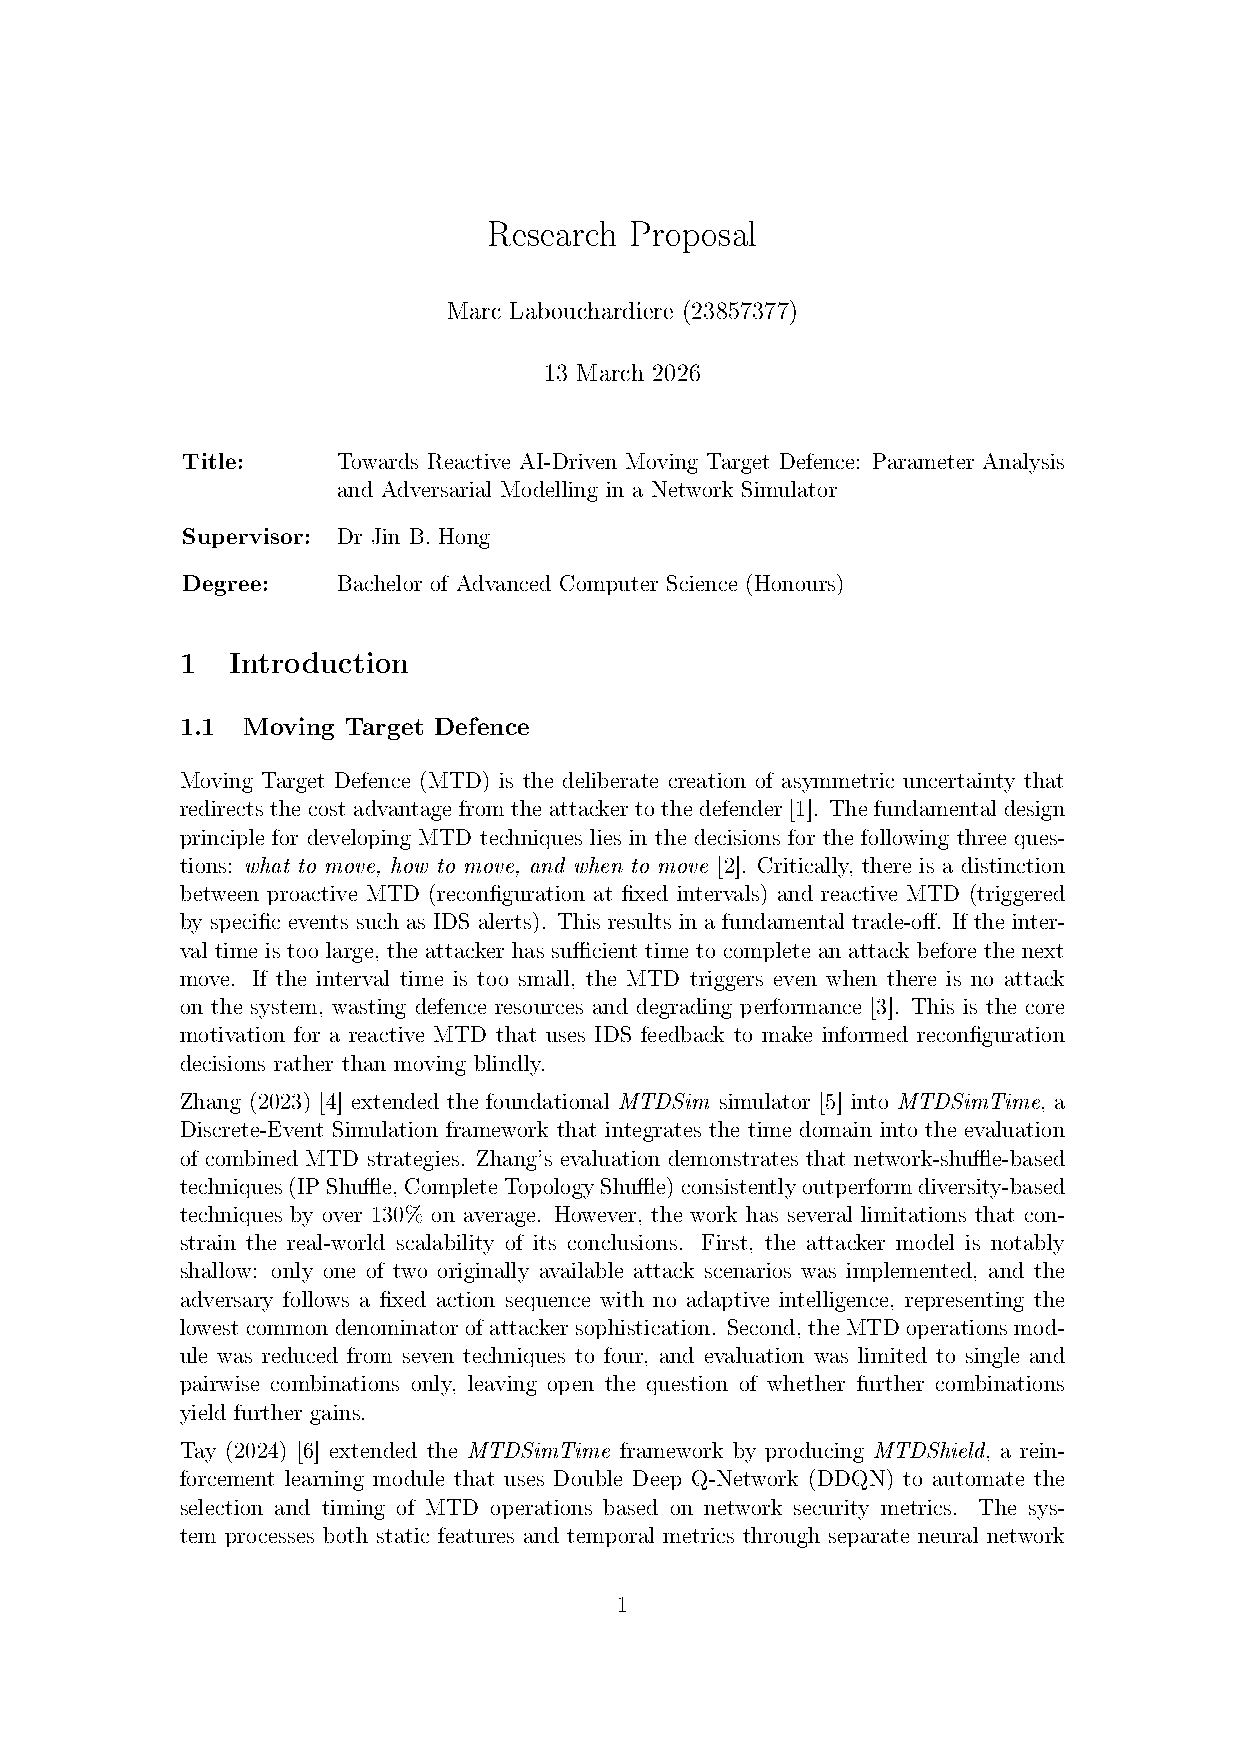
\includepdf[pages=-]{proposal.pdf}


% =====================================================================
% APPENDIX B, REBUILT 2026-10-04 (Marc: "the appendix ... I don't want it to
% just be a wasteland ... reasonably polished ... useful ... of interest to
% the examiner"; "it was drafted before we standardised all the terms").
% One section per Chapter 4 claim, in the chapter's order (4.1, 4.2, 4.4.2,
% 4.4.3, 4.4.4); each opens with one or two sentences naming the claim it
% backs, and its floats sit under it (\FloatBarrier at each section's end).
% Headings in the chapter's terms (no "both resolutions", no lead "objective").
% Moved in: Appendix D (the mining table) as B.1. Cut, history in git:
% "Partition schemes considered" (unreferenced since the 4.2 redraft; it
% answered a question 4.2 no longer asks), the anchor-families table (4.4.2
% says it), the full failure-matrix table (Figure B.6(c) cell for cell), the
% distance-kernel bands figure (the Appendix C.3 table's caption carries its
% one finding, that the floor never binds), and the typed Experiment 1 table (replaced by
% the generated total-mapping table, the run Table C.1 cites). Every float is
% generated; the generators are named in each float file's header.
% DRAFT STATE: openers and captions session-drafted, ratify on read.
\chapter{Supplementary material for the APT attacker model}
\label{app:movement}

Each section of this appendix backs one claim of
Chapter~\ref{ch:attacker-model}, in the chapter's order.

% Mining: was Appendix D (label kept, cited from 4.1). Two failures worth a
% clause if the opener ever needs an example, both off the run log and
% neither threshold-sensitive: keyword mining read T1110's cross-reference to
% Valid Accounts as a precondition, direction inverted; T1059 was the source
% of 24 of the 42 co-occurrence edges because it is the most used technique,
% not because anything depends on it. No mining threshold is printed: the
% April parameters cannot be sourced (gap_schema.md Decision 1).
\section{Edges from co-occurrence and keyword mining}
\label{app:cooccurrence}

Table~\ref{tab:preliminary-extraction} gives the edges between tactics that
co-occurrence mining, keyword mining and the attack flows found
(Section~\ref{sec:technique-graph}), and why the two mining methods were not
used.

% GENERATED by tools/preliminary_extraction_table.py --- do not hand-edit.
% Numbers: data/gap/archive/v0_4_extraction_run.json (computed from the v0.4 GAP
%   on archive/attacker-profiling and from data/gap/gap_v0.5.json).
% Wording: data/gap/archive/preliminary_extraction_labels.json.
% DRAFT STATE (2026-10-04 appendix pass): caption session-drafted, ratify on read.
% Requires booktabs (already in the preamble).

\begin{table}[htbp]
\centering
\caption[Edges between tactics found by mining and by attack flows]{Three ways of finding the edges between tactics (Section~\ref{sec:technique-graph}), run in one earlier build of the attack graph (2026-04-19) over the same ATT\&CK techniques. \emph{Edges between tactics} counts the ordered pairs of different tactics each found, of the 182 that ATT\&CK's 14 tactics then allowed.}
\label{tab:preliminary-extraction}
\tablestyle
\begin{tabular}{@{}P{0.13\textwidth} P{0.20\textwidth} P{0.14\textwidth} r P{0.26\textwidth}@{}}
\toprule
Way & An edge rests on & Direction from & \shortstack[r]{Edges between\\tactics} & Why it was not used \\
\midrule
Co-occurrence mining & the same APT group or tool uses both techniques & an assumed order of the tactics & 19 (10\,\%) & Using two techniques together says nothing about which came first, and an assumed order allows no edge back. \\
Keyword mining & one technique's ATT\&CK description names the other & an assumed order of the tactics & 25 (14\,\%) & A description that names another technique refers to it; it does not say the attacker needs it first. \\
\textbf{Attack flows} & an analyst drew one step after the other & the analyst's drawing & 91 (50\,\%) & Adopted. \\
\bottomrule
\end{tabular}
\end{table}

\FloatBarrier

% Figures generated by tools/gap_appendix_figures.py from data/gap/gap_v0.5.json
% and data/gap/flows/; regenerate, never hand-edit. 419/478 and 47/122 recomputed
% from gap_v0.5.json on 2026-10-04 (flow_ids per edge; tactic edges exclude
% steps within a tactic, as 4.1 defines).
\section{Techniques or tactics as the nodes of the attack graph}
\label{app:full-graph}

Section~\ref{sec:technique-graph} chose tactics as the nodes of the attack
graph because most edges between techniques come from one attack flow: 419
of the 478 (88\,\%), against 47 of the 122 edges between tactics (39\,\%).
Figure~\ref{fig:app-flow-exemplar} shows one attack flow;
Figures~\ref{fig:app-technique-graph} to~\ref{fig:app-tactic-graph}
aggregate all 38, with techniques as nodes and then tactics.

\begin{figure}[p]
  \centering
  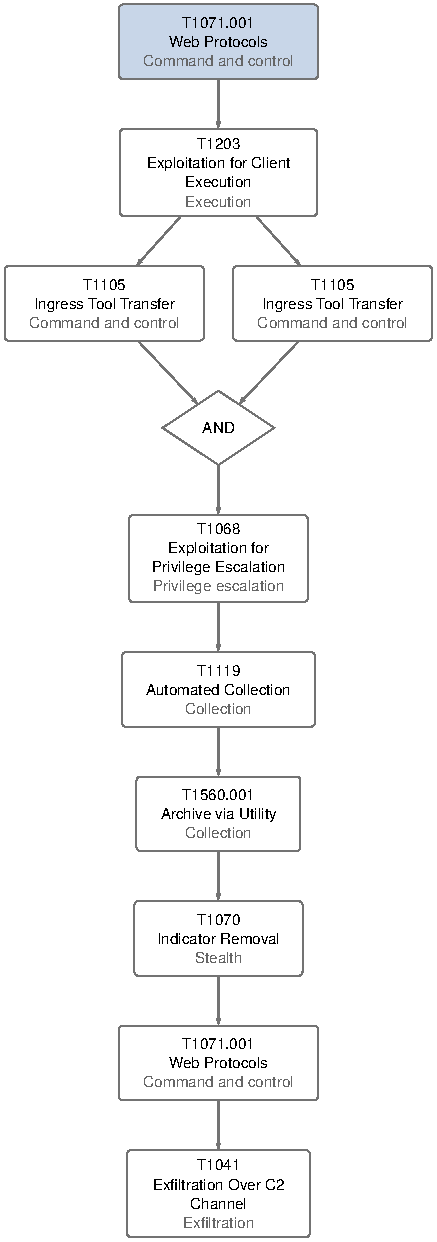
\includegraphics{fig_B-1a_gap_flow_exemplar}
  \caption[One attack flow as its analyst drew it]{One attack flow as its
  analyst drew it: CISA AA22-138B, VMware Workspace ONE (TA1), from the
  Attack Flow corpus. Each box gives a technique's identifier and name and,
  in grey, its tactic; the filled box is the first step. Both steps into the
  diamond (an AND) come before the step after it.}
  \label{fig:app-flow-exemplar}
\end{figure}

\begin{landscape}
\begin{figure}[p]
  \centering
  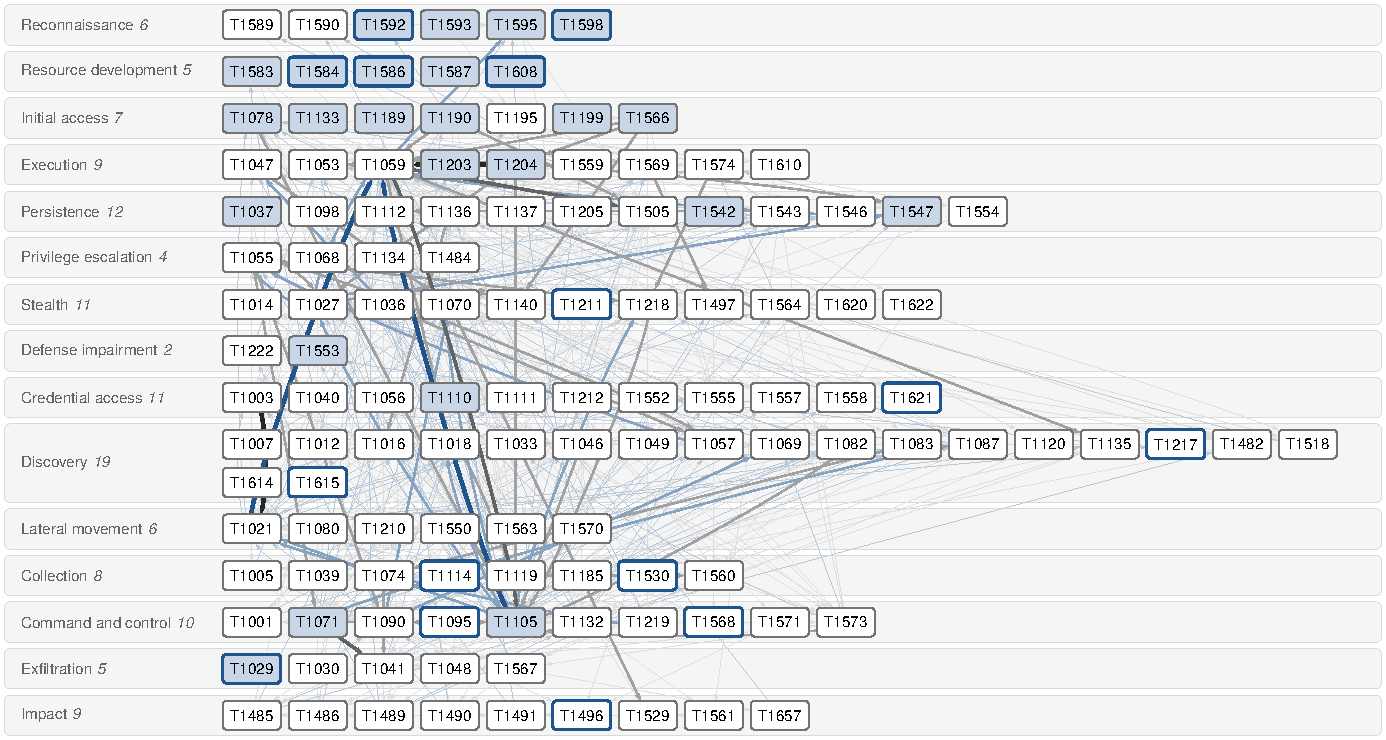
\includegraphics{fig_B-1b_gap_technique_graph}
  \caption[The attack graph with techniques as nodes]{The attack graph with
  techniques as nodes: 124 techniques and 478 edges from the 38 attack flows.
  Techniques are grouped by tactic, in ATT\&CK matrix order, and labelled by
  identifier; each group gives its tactic and, in italic, how many of its
  techniques the attack flows use. Darker, thicker edges are drawn by more
  attack flows, up to four; blue edges run back to an earlier tactic. A
  filled box is a technique some attack flow starts at, and a blue-outlined
  box one some attack flow ends at.}
  \label{fig:app-technique-graph}
\end{figure}
\end{landscape}

\begin{landscape}
\begin{figure}[p]
  \centering
  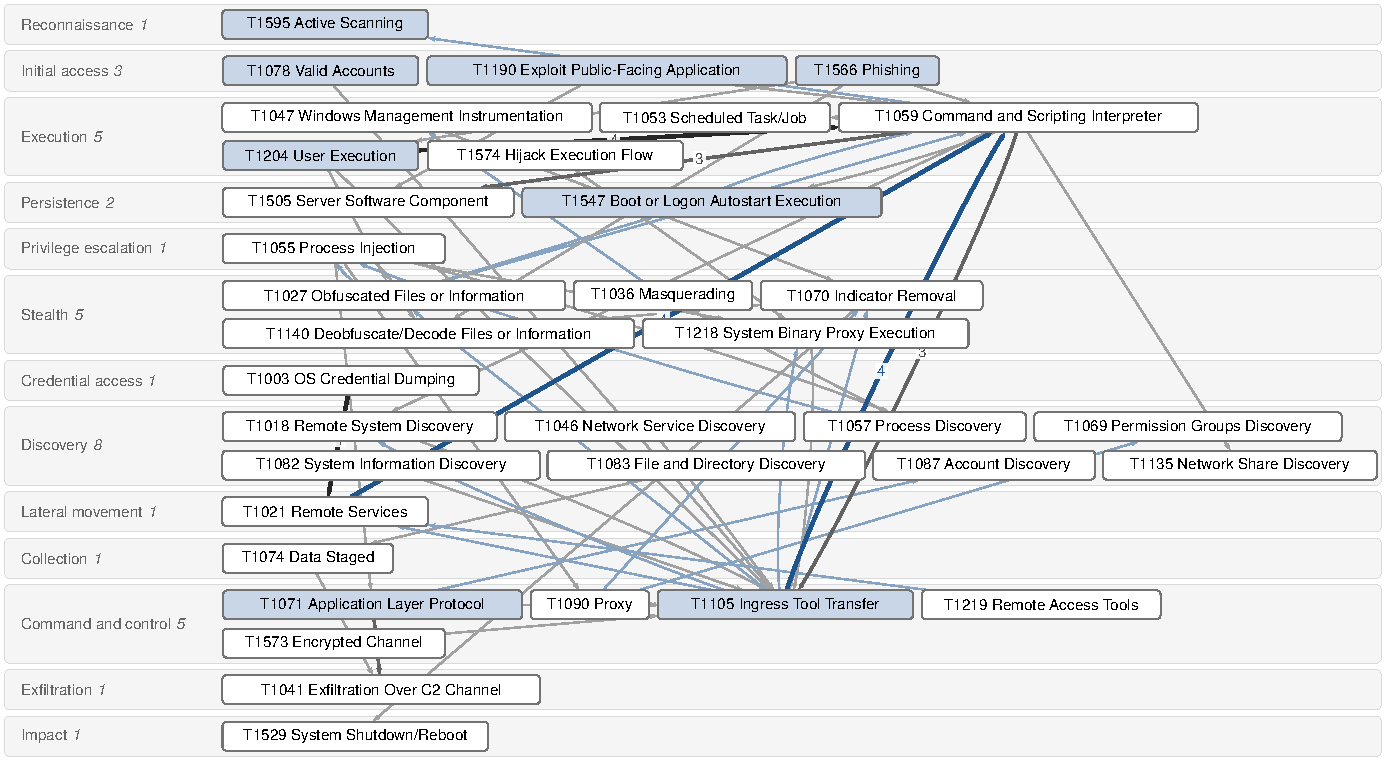
\includegraphics{fig_B-1c_gap_technique_core}
  \caption[The attack graph with techniques as nodes, edges from two or more
  attack flows]{The attack graph of Figure~\ref{fig:app-technique-graph}
  with only the edges drawn by two or more attack flows, and without the
  pieces of fewer than three techniques this leaves: 35 techniques and 55
  edges. A number on an edge counts the attack flows that drew it, where more
  than two did.}
  \label{fig:app-technique-core}
\end{figure}
\end{landscape}

\begin{landscape}
\begin{figure}[p]
  \centering
  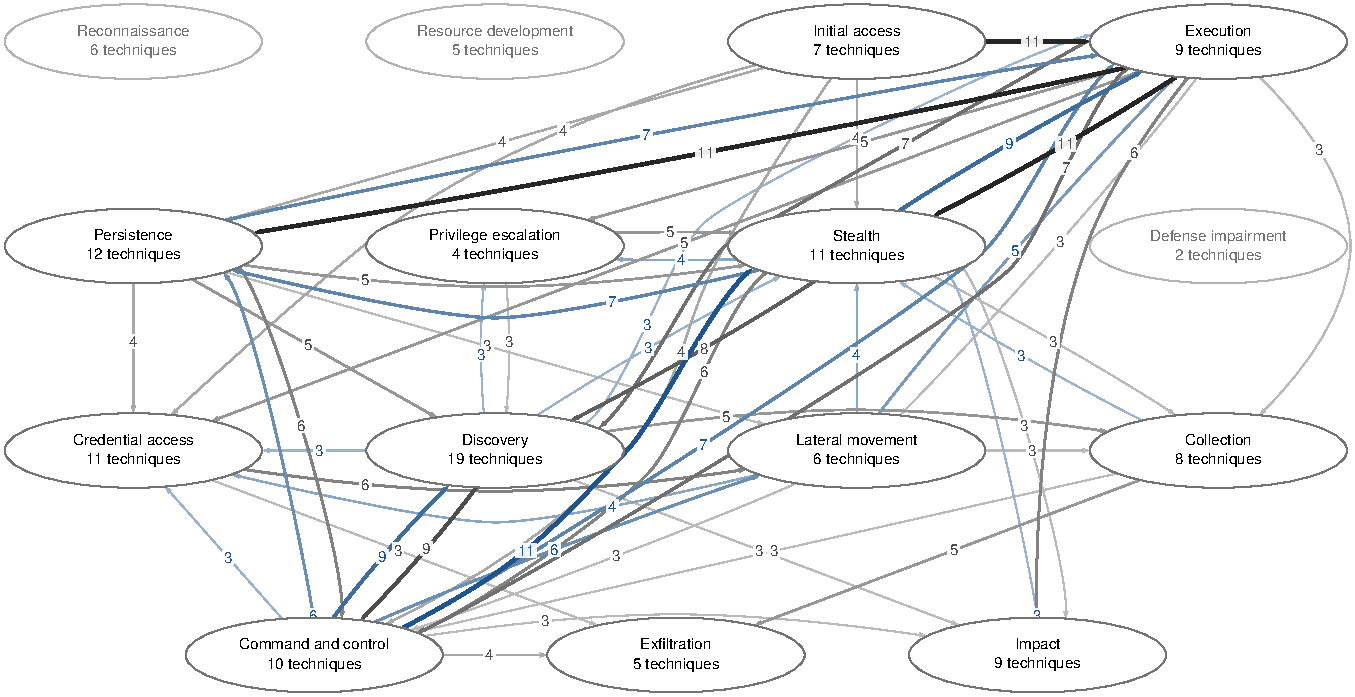
\includegraphics{fig_B-1d_gap_tactic_graph}
  \caption[The attack graph with tactics as nodes]{The attack graph with
  tactics as nodes, as Chapter~\ref{ch:attacker-model} uses it: the 55 of its
  122 edges drawn by three or more attack flows. Each tactic gives the number
  of techniques the attack flows use for it. Darker, thicker edges are drawn
  by more attack flows, up to 11; blue edges run back to an earlier tactic.
  Reconnaissance, resource development and defense impairment, in grey, have
  no edge drawn by three or more.}
  \label{fig:app-tactic-graph}
\end{figure}
\end{landscape}
\FloatBarrier

% Table generated by tools/gasp_structural_baseline.py --tex from
% data/gasp/metadata_audit.csv. The three decisions are the audit's
% marc_ruling_2026-08-17 rows, each read against its cited threat report.
\section{The attack profile of each attack flow}
\label{app:classification-audit}

Table~\ref{tab:profile-sources} gives the sources that answered the two
questions of Section~\ref{sec:attack-profiles} for each attack flow. We
decided the three attack flows these sources left open from their threat
reports. CISA AA22-138B VMWare Workspace (Alt) draws a script that the advisory says steals
sensitive data, so its attacker stole data \citep{cisaaa22138b}. Mac Malware
Steals Crypto stole credentials and also mined cryptocurrency on the victims'
machines, hijacking them, so it did both \citep{unit42maccookies2019}.
SearchAwesome Adware injects adverts but, by its report, does not take user
data, and it impedes no system, so it did neither \citep{malwarebytesadware2018}.

% GENERATED by tools/gasp_structural_baseline.py --tex from
%   data/gasp/metadata_audit.csv (classification and sources read) and
%   data/gap/flows/*.yaml (the analyst's own citation list, carried through from
%   the tracked corpus bundles in data/gap/_corpus_stix/).
% Do not hand-edit; regenerate. DRAFT STATE (2026-10-04 appendix pass): caption
%   session-drafted, ratify on read.
% At generation: 38 attack flows, 3 decided by the author.

\begin{table}[htbp]
\centering
\caption[The sources that answered each attack flow]{The sources that answered the two questions of Section~\ref{sec:attack-profiles} for each attack flow, grouped by attack profile (Table~\ref{tab:attack-profiles}). The CTID description of every attack flow was read \citep{ctid2025attackflow}; the columns give what else was. \emph{Step notes} are the analyst's notes on the steps of the attack flow. \emph{ATT\&CK group} is the group page read \citep{mitre2026attackv19}. \emph{Decided by us} marks the attack flows these sources left open.}
\label{tab:profile-sources}
\tablestyle
\begin{tabular}{@{}P{0.38\textwidth}ccP{0.17\textwidth}c@{}}
\toprule
Attack flow & \shortstack{Step\\notes} & \shortstack{ATT\&CK\\group} & Threat report & \shortstack{Decided\\by us} \\
\midrule
\grouprow{5}{$c_{1}$ (19 attack flows)} \\
CISA AA22-138B VMWare Workspace (Alt) & \propmet &  & \citep{cisaaa22138b} & \propmet \\
CISA AA22-138B VMWare Workspace (TA1) & \propmet &  & \citep{cisaaa22138b} &  \\
Cobalt Kitty Campaign &  &  & \citep{cybereasoncobaltkitty} &  \\
Equifax Breach &  &  & \citep{csoequifax2020} &  \\
FIN13 Case 1 &  & G1016 &  &  \\
FIN13 Case 2 &  & G1016 &  &  \\
Ivanti Vulnerabilities &  &  & \citep{volexityivanti2024} &  \\
JP Morgan Breach &  &  &  &  \\
Marriott Breach &  &  &  &  \\
MITRE NERVE &  &  & \citep{engenuitynerve} &  \\
Muddy Water & \propmet & G0069 & \citep{talosmuddywater2022} &  \\
OceanLotus &  & G0050 &  &  \\
SolarWinds &  & G0016 &  &  \\
SWIFT Heist &  & G0082 &  &  \\
Target Breach &  &  &  &  \\
ToolShell Vulnerability in Sharepoint & \propmet &  & \citep{unit42sharepoint2025} &  \\
Turla - Carbon Emulation Plan &  & G0010 &  &  \\
Turla - Snake Emulation Plan &  & G0010 &  &  \\
Uber Breach & \propmet & G1004 & \citep{uberbreach2022} &  \\
\midrule
\grouprow{5}{$c_{2}$ (7 attack flows)} \\
CISA Iranian APT &  &  &  &  \\
Maastricht University Ransomware &  &  &  &  \\
NotPetya &  & G0034 &  &  \\
Shamoon &  &  & \citep{mcafeeshamoon} &  \\
Sony Malware &  & G0032 &  &  \\
Tesla Kubernetes Breach &  &  &  &  \\
WhisperGate &  & G0034 &  &  \\
\midrule
\grouprow{5}{$c_{3}$ (7 attack flows)} \\
Black Basta Ransomware &  &  & \citep{unit42basta2022} &  \\
Conti CISA Alert &  & G0102 &  &  \\
Conti PWC &  & G0102 &  &  \\
Conti Ransomware &  & G0102 &  &  \\
Mac Malware Steals Crypto & \propmet &  & \citep{unit42maccookies2019} & \propmet \\
Ragnar Locker &  & G0125 &  &  \\
REvil &  & G0115 &  &  \\
\midrule
\grouprow{5}{$c_{4}$ (5 attack flows)} \\
CISA AA22-138B VMWare Workspace (TA2) & \propmet &  & \citep{cisaaa22138b} &  \\
DFIR - BumbleBee Round 2 &  &  & \citep{dfirbumblebee2022} &  \\
Gootloader &  &  & \citep{dfirgootloader2022} &  \\
Hancitor DLL &  &  & \citep{dfirdomainadmin2021} &  \\
SearchAwesome Adware & \propmet &  & \citep{malwarebytesadware2018} & \propmet \\
\bottomrule
\end{tabular}
\end{table}

\FloatBarrier

\section{Edges of the attack profiles}
\label{app:profile-edges}

Each attack profile's Petri net takes only the edges its own attack flows
drew (Section~\ref{sec:attack-profiles}); Figure~\ref{fig:profile-edges}
gives them.

% Generated by tools/ch4_attack_profiles_figure.py; the build fails if a
% panel drifts from its Petri net's flow-backed transitions.
\begin{figure}[htbp]
  \centering
  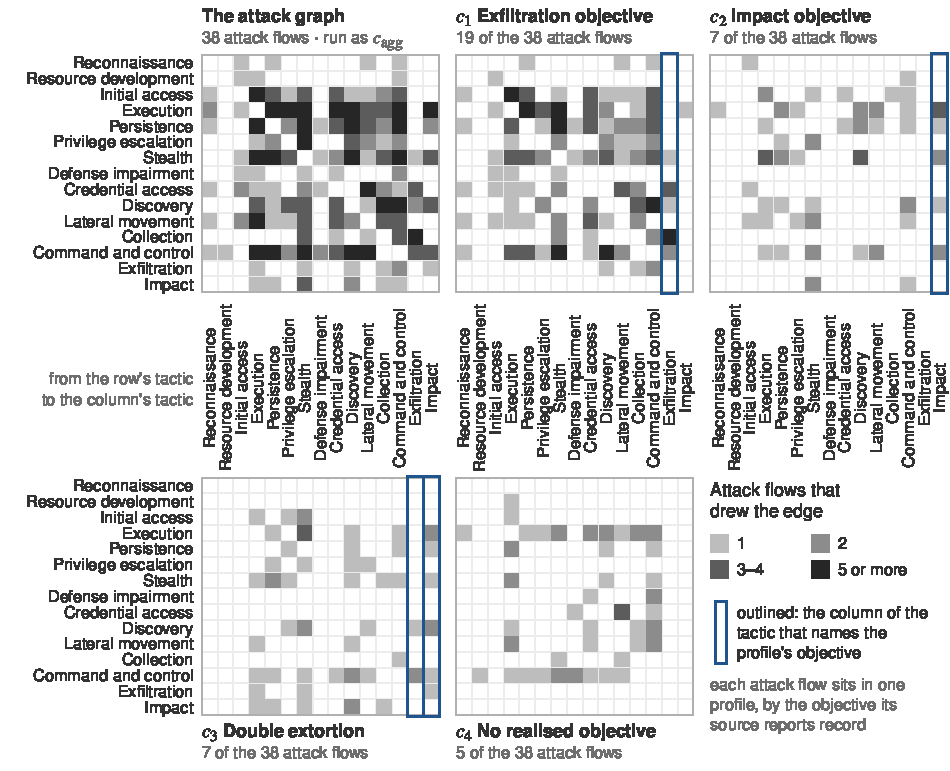
\includegraphics{fig_4-2a_attack_profiles}
  \caption[Edges of the four attack profiles]{Edges of the four attack
  profiles: each cell is an edge from the tactic of its row to the tactic of
  its column, darker where more of the attack profile's attack flows draw it.
  Exfiltration is outlined where the attackers stole data, and impact where
  they impeded systems (Table~\ref{tab:attack-profiles}).}
  \label{fig:profile-edges}
\end{figure}
\FloatBarrier

% Table generated by tools/dwell_catalogue_tables.py from
% data/ogasp/tactic_durations.json (reasons: short_justification, reworded
% 2026-10-04 in the chapter's terms).
\section{How each tactic duration was set}
\label{app:dwell-derivation}

Table~\ref{tab:dwell-derivation} gives the reference value, multiplier and
band of each mean duration of Section~\ref{subsec:dwell-times}, and the reason
for each.

% GENERATED by tools/dwell_catalogue_tables.py from
%   data/ogasp/tactic_durations.json (v0-uncalibrated); tactic axis and
%   display names from the pinned ATT&CK bundle (v19.1).
% Do not hand-edit; regenerate. Requires booktabs (already in the preamble).

\begin{table}[htbp]
\centering
\caption[How each tactic duration was set]{How each tactic duration of Table~\ref{tab:dwell-catalogue} was set (Section~\ref{subsec:dwell-times}): a reference value, in brackets, times the tactic's multiplier. \emph{Band} is the declared range of the multiplier.}
\label{tab:dwell-derivation}
\tablestyle
\begin{tabular}{@{}P{0.15\textwidth} P{0.13\textwidth} r r c P{0.29\textwidth}@{}}
\toprule
Tactic & Reference (s) & Multiplier & Duration (s) & Band & Reason \\
\midrule
Reconnaissance & Scans' total (35.0) & 1.0 & 35.0 & [0.5, 2] & Surveys a network, as MTDSim's three scans do together; the band allows slower, staged reconnaissance. \\
Resource development & --- & --- & 0.0 & --- & Happens off the target's network, out of the defender's sight, so it takes no simulated time. \\
Initial access & Exploit's median (4.5) & 1.0 & 4.5 & [0.5, 2] & Exploiting a public-facing service, which MTDSim's exploit already times. \\
Execution & Judgement (45.0) & 0.5 & 22.5 & [0.1, 2] & Quick in itself but paced to stay hidden, so half of 45 s, with a band that leans fast. \\
Persistence & Judgement (45.0) & 1.0 & 45.0 & [0.25, 4] & Keeping a foothold through reboots is quiet holding work, which no attack action costs. \\
Privilege escalation & Exploit's median (4.5) & 1.0 & 4.5 & [0.5, 2] & Usually a vulnerability exploit; the band runs from an exploit to reusing a stolen token. \\
Stealth & Judgement (45.0) & 1.0 & 45.0 & [0.25, 4] & A pace the attacker keeps throughout the attack. \\
Defense impairment & Judgement (45.0) & 0.5 & 22.5 & [0.1, 4] & A short act before a noisy payload, so half of 45 s; attackers prefer to evade defences, so the band is wide. \\
Credential access & Exploit's median (4.5) & 1.0 & 4.5 & [0.5, 2] & Dumping and cracking credentials is on-host work like an exploit; stealing a ticket is faster. \\
Discovery & Scans' total (35.0) & 1.0 & 35.0 & [0.5, 2] & The enumeration of reconnaissance, run from inside a foothold. \\
Lateral movement & Exploit's median (4.5) & 1.0 & 4.5 & [0.25, 4] & Usually a remote login, costed as an exploit; the band is wide because a worm moves fast and a person slowly. \\
Collection & Judgement (36.0) & 1.0 & 36.0 & [0.5, 2] & Gathering data, from a quick grab to a slow harvest. \\
Command and control & Judgement (45.0) & 1.0 & 45.0 & [0.25, 4] & A quiet channel that beacons on a cadence, not one act. \\
Exfiltration & Judgement (36.0) & 1.0 & 36.0 & [0.25, 4] & Sending the data out, from a fast bulk transfer to a slow trickle. \\
Impact & Judgement (36.0) & 1.0 & 36.0 & [0.1, 5] & Encrypting, destroying or hijacking systems; these payloads vary most in time, so the band is the widest. \\
\bottomrule
\end{tabular}
\end{table}

\FloatBarrier

% Table generated by tools/controller_mapping_figure.py, the generator of
% Figure 4.6, so the two cannot disagree. Record:
% docs/implementation/pipeline/ogasp/controller_mapping_v2.md.
\section{Reasons for the tactic-to-action mapping}
\label{app:controller-mapping}

Table~\ref{tab:controller-mapping} gives the reason for each row of the
tactic-to-action mapping of Section~\ref{subsec:tactic-verb-mapping}. A
tactic is unmapped where the simulator has nothing for it to act on.

% GENERATED by tools/controller_mapping_figure.py --- do not hand-edit.
\begin{table}[htbp]
\centering
\caption[Reasons for the tactic-to-action mapping]{The reason for each row of the tactic-to-action mapping (Figure~\ref{fig:controller-mapping}), grouped by lifecycle stage: for a direct pair, the ATT\&CK technique its attack action carries out; for a broad pair, what the two share; for an unmapped tactic, marked by a dash, what MTDSim lacks.}
\label{tab:controller-mapping}
\tablestyle
\begin{tabular}{@{}l l P{0.52\textwidth}@{}}
\toprule
Tactic & Attack action & Reason \\
\midrule
\grouprow{3}{preparation} \\
Reconnaissance & scan host & Active Scanning: finds the hosts the attacker can attack from its current host. \\
Resource development & --- & Building tools happens off the target's network, which MTDSim does not model. \\
\midrule
\grouprow{3}{intrusion} \\
Initial access & exploit & Exploit Public-Facing Application: the only attack action that gives the attacker a host it did not hold. \\
Execution & exploit & Exploitation for Client Execution: an exploit is MTDSim's only way to run the attacker's code on a host. \\
\midrule
\grouprow{3}{post-intrusion operations} \\
Persistence & --- & A compromised host stays compromised, so there is no foothold to keep. \\
Privilege escalation & exploit & Exploitation for Privilege Escalation: MTDSim has no privilege levels, so each further exploit brings a host closer to compromise instead. \\
Stealth & --- & Nothing in MTDSim watches the attacker, so there is nothing to hide from. \\
Defense impairment & --- & The MTD schedule runs on the defender's side; the attacker can neither see nor change it. \\
Credential access & brute force & Brute Force: tries the usernames already stolen against the current host. \\
Discovery & scan port & Network Service Discovery: lists the open ports of the current host, which a later exploit needs. \\
Lateral movement & enumerate host & Broad: enumerating a host moves the attacker to its next host, as lateral movement does. \\
Command and control & scan neighbours & Broad: Brown describes this attack action as command and control revealing connected hosts \citep{brown2023}. \\
\midrule
\grouprow{3}{actions on objectives} \\
Collection & --- & Hosts in MTDSim carry services and vulnerabilities, but no data to gather. \\
Exfiltration & --- & There is no data to take, and nowhere outside the network to send it. \\
Impact & --- & No attack action encrypts, destroys or hijacks a system, so the tactic only takes time. \\
\bottomrule
\end{tabular}
\end{table}

\FloatBarrier

% Table generated by tools/total_mapping_table.py from
% data/results/ch5_s51_sensitivity/numbers.json (the run Table C.1 cites;
% record: ch5_s51_sensitivity_findings.md section 5). The numbers in the
% opener are that table's no-MTD row.
\section{A total tactic-to-action mapping}
\label{app:experiment-one}
% [2026-10-05, Section 4.4.1 round 3: no longer cited from Section 4.4.1
%  (Marc: the mapping is argued from what the attack actions carry out).
%  Kept because Appendix C's Tables C.0a and C.0b cite it as the mapping's
%  alternative; whether to cut it there is Marc's ruling.]

A total mapping gives every tactic an attack action, so the APT attacker
model takes the baseline attacker's attack actions in a stochastic order.
The baseline attacker runs them in a fixed order, each meeting the
precondition of the next; out of that order most are refused, and the
attacker reaches 0.15 hosts without MTD, against 8.13 under the partial
mapping of Figure~\ref{fig:controller-mapping}
(Table~\ref{tab:experiment-one}).

% GENERATED by tools/total_mapping_table.py from
%   data/results/ch5_s51_sensitivity/numbers.json (the mapping block). Do not
%   hand-edit; regenerate. DRAFT STATE (2026-10-04 appendix pass): caption
%   session-drafted, ratify on read.
\begin{table}[htbp]
\centering
\caption[The total tactic-to-action mapping against the partial one]{The APT attacker model under the partial tactic-to-action mapping and under a total one, with its four attack profiles pooled (400 runs per row). \emph{Refused} is the share of attack actions the simulator turned down because their precondition was not met. Intervals are 95\,\%.}
\label{tab:experiment-one}
\tablestyle
\begin{tabular}{@{}l r r r@{}}
\toprule
Mapping & Distinct hosts reached & Attack actions & Refused (\%) \\
\midrule
\grouprow{4}{No MTD} \\
Partial (Figure~\ref{fig:controller-mapping}) & $8.13 \pm 0.42$ & 317 & 24 \\
Total & $0.15 \pm 0.04$ & 504 & 58 \\
\midrule
\grouprow{4}{Random deployment strategy, 200\,s interval} \\
Partial (Figure~\ref{fig:controller-mapping}) & $2.07 \pm 0.19$ & 347 & 63 \\
Total & $0.09 \pm 0.03$ & 535 & 95 \\
\midrule
\grouprow{4}{Random deployment strategy, 2\,000\,s interval} \\
Partial (Figure~\ref{fig:controller-mapping}) & $7.42 \pm 0.38$ & 324 & 33 \\
Total & $0.12 \pm 0.03$ & 507 & 83 \\
\bottomrule
\end{tabular}
\end{table}

\FloatBarrier

% Tables and figure generated by tools/failure_weight_decomposition_figure.py
% from data/ogasp/controller/{outcome_rules,lifecycle_consensus}.json through
% the tracked compiler (overlay v4_failure_only). Record:
% docs/implementation/pipeline/ogasp/failure_weight_decomposition.md.
\section{The rules of the failure matrix}
\label{app:weight-sets}

Each value of the failure matrix of Section~\ref{subsec:failure-matrix} is
a rule value times a distance factor. Table~\ref{tab:overlay-failure-rules}
gives the rules, Table~\ref{tab:overlay-distance-kernel} the distance factor,
and Figure~\ref{fig:failure-weight-decomposition} draws both and their
product.

% GENERATED by tools/failure_weight_decomposition_figure.py from
%   data/ogasp/controller/outcome_rules.json + lifecycle_consensus.json
%   through mtdsim.l3_simulation.controller.rules (overlay version v4_failure_only).
% Do not hand-edit; regenerate. Requires booktabs + graphicx (both in the preamble).

\begin{table}[htbp]
\centering
\caption[The rules of the failure matrix]{The rules that set the failure matrix (Section~\ref{subsec:failure-matrix}). After a failure at one tactic, the first rule that matches the move to the next tactic gives its value, which the distance factor of Table~\ref{tab:overlay-distance-kernel} then scales. Back, within and forward are by lifecycle stage. The letters are those of Figure~\ref{fig:failure-weight-decomposition}(a).}
\label{tab:overlay-failure-rules}
\tablestyle
\begin{tabular}{@{}c P{0.40\textwidth} r P{0.40\textwidth}@{}}
\toprule
Rule & Applies to & Value & Reason \\
\midrule
A & After a failed initial access, a move to a tactic that needs a foothold & 0.02 & No foothold was gained, so these moves are almost out of reach. \\
B & After a failed reconnaissance, a move to initial access & 0.4 & Nothing was found, so breaking in is harder but still possible. \\
C & After a failed reconnaissance, a move to a tactic that needs a foothold & 0.05 & With no foothold, a move deep into the network is implausible. \\
D & After a failure with a foothold, a move back to a tactic without one & 0.25 & Falling right back to before the foothold is an uncommon response. \\
E & Any other move back to execution & 0.35 & Running code again on a held foothold continues the attack. \\
F & Any other move back: from initial access to preparation, or from actions on objectives to post-intrusion operations & 0.9 & Going back one stage is the common response to a failure. \\
G & A move within the same stage & 0.7 & Another tactic of the stage is an alternative route. \\
H & A move forward, with a foothold & 0.35 & Advancing straight after a failure is possible but uncommon. \\
I & A move forward, without a foothold & 0.3 & The step the next one depends on did not succeed. \\
\bottomrule
\end{tabular}
\end{table}

% No success-rules table and no success-set table for v4_failure_only:
%   the success table of this version is the multiplicative identity (every
%   cell 1.0, rule `passthrough`) — on a success verdict the token routes on
%   the corpus proportions unchanged, and only the failure table is declared.
%   The retired success rules remain in outcome_rules.json, unconsulted.

\begin{table}[htbp]
\centering
\caption[The distance factor of the failure matrix]{The distance factor that scales each rule value by the lifecycle stages a move crosses. A move within a stage or to the next keeps its rule value; each further stage forward multiplies it by $\gamma$, and each further stage back by $\delta$. A factor below $z$ is zero. Appendix~\ref{app:decay-robustness} moves each parameter across its band.}
\label{tab:overlay-distance-kernel}
\tablestyle
\begin{tabular}{@{}l r l@{}}
\toprule
Parameter & Value & Band \\
\midrule
$\gamma$, forward & 0.25 & \{0.1, 0.5\} \\
$\delta$, back & 0.25 & \{0.1, 0.5\} \\
$z$, floor & 0.1 & \{0, 0.05, 0.1\} \\
\bottomrule
\end{tabular}
\end{table}


\begin{figure}[p]
  \centering
  % scoped to this float: the full-page box lands 2--3pt over \textheight at
  % the class default skip; the panels are NOT scaled down to make room.
  \setlength{\abovecaptionskip}{6pt}
  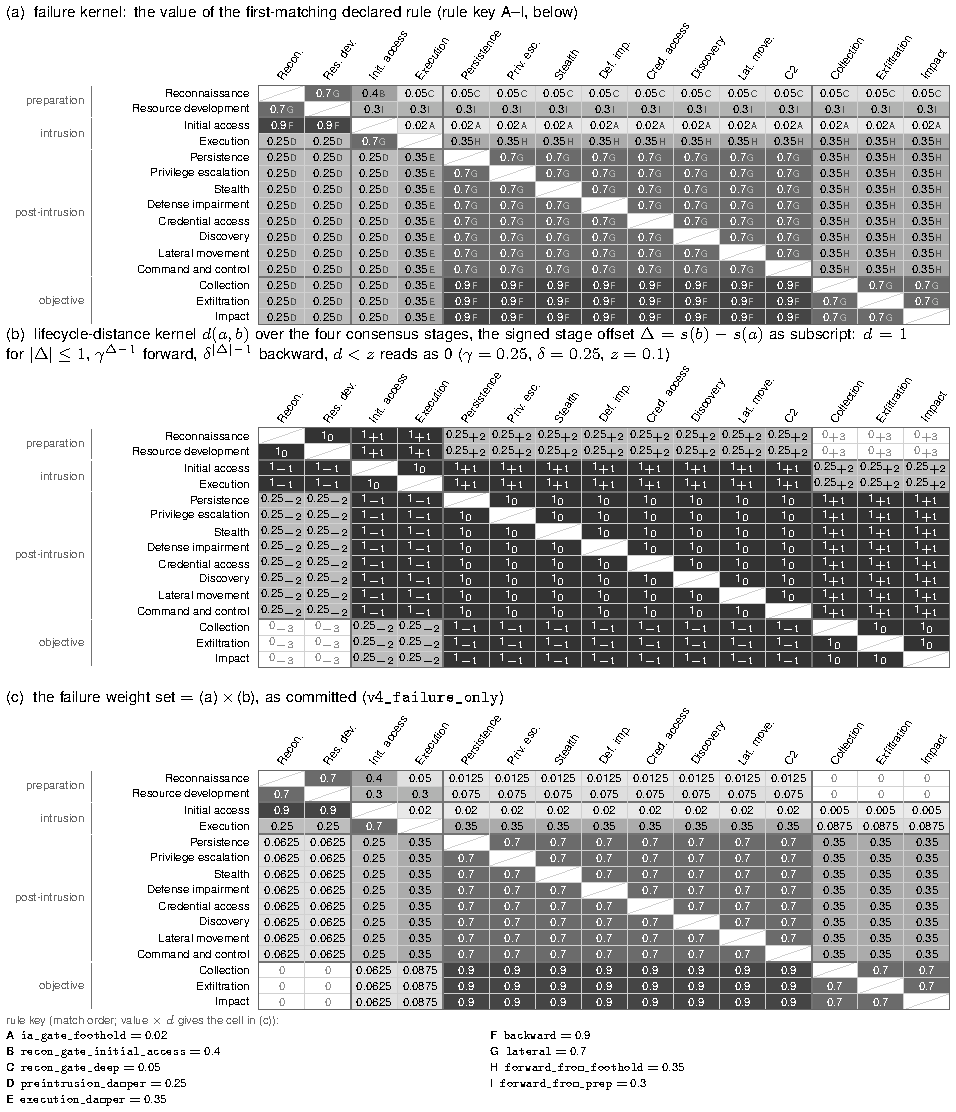
\includegraphics[width=\textwidth]{fig_B-6a_failure_weight_decomposition}
  \caption[The failure matrix as rule value times distance factor]{The
  failure matrix~(c) as the product of the rule value~(a) and the distance
  factor~(b). Rows are the tactic whose attack action failed and columns the
  candidate next tactic, grouped by lifecycle stage; one grey scale from 0
  to~1 serves all three panels. (a)~The value of the first rule that matches
  each move, with its letter (Table~\ref{tab:overlay-failure-rules}).
  (b)~The distance factor (Table~\ref{tab:overlay-distance-kernel}), with the
  number of stages the move crosses as subscript, negative for a move back.
  (c)~The failure matrix.}
  \label{fig:failure-weight-decomposition}
\end{figure}
\FloatBarrier


% Completed sensitivity sweeps too verbose for the results preamble; the
% ~200-value success/failure overlay matrix declaration (V6: per-user
% adoption concern, not a swept dimension).
\chapter{Supplementary sensitivity analyses}
\label{app:sensitivity}

% LEAD DRAFT STATE 2026-09-20 --- connective prose (green-lit), ratify-on-read.
% Was the lead of C.1 pointing at the body's Table 5.1; the table now leads the
% appendix (the body section was cut, see the note at the head of ch5).
% [2026-10-04: the bases table added first, the four-bases list of the 4.4
%  preamble as a table (generated, tools/value_bases_table.py). DRAFT STATE.]
Every value of the APT attacker model comes from one of four bases: the Attack
Flow corpus, MTDSim's own attack-action times, the literature or our judgement.
Table~\ref{tab:value-bases} lists each value with its basis, where its reason is
given and the test that varies or removes it. Three values of our judgement are
not tested: the per-tactic duration multipliers, the overlay's share and the
choice of one attack flow per APT group.
Table~\ref{tab:parameter-register} lists the values chosen for the attacker
model in Section~\ref{sec:execution} and what happened when each was moved, at
the configuration of Section~\ref{sec:dimensions}. The sections that follow
read the same perturbations value by value.

% GENERATED by tools/value_bases_table.py from data/ogasp/value_bases.json --- do not hand-edit.
% DRAFT STATE (2026-10-04, 4.4 preamble redraft): caption session-drafted, ratify on read.
\begin{table}[htbp]
  \centering
  \caption[Each value of the APT attacker model and its basis]{Each value of
  the APT attacker model, grouped by its basis, with where its reason is given
  and the test that varies, substitutes or removes it. A blank test cell: the
  value is not varied.}
  \label{tab:value-bases}
  \tablestyle
  \begin{tabular}{@{}P{2.2cm}P{5.2cm}P{2.6cm}P{4.4cm}@{}}
    \toprule
    Basis & Value & Reason & Tested \\
    \midrule
    Corpus & Base weights of the Petri nets & Section~\ref{sec:petri-formalism} &  \\
     & Membership of each attack profile & Section~\ref{sec:attack-profiles} &  \\
    \addlinespace
    MTDSim & Scan-shaped and exploit-shaped tactic durations & Section~\ref{subsec:dwell-times} & varied, Appendix~\ref{app:dwell-robustness} \\
     & Confusion penalty & Section~\ref{subsec:attacker-model} &  \\
    \addlinespace
    Literature & Order of the lifecycle stages & Section~\ref{subsec:apt} &  \\
    \addlinespace
    Our judgement & Low-and-slow and objective-execution tactic durations & Table~\ref{tab:dwell-derivation} & varied, Appendix~\ref{app:dwell-robustness} \\
     & Per-tactic duration multipliers & Table~\ref{tab:dwell-derivation} & not tested \\
     & Exponential draw & Section~\ref{subsec:dwell-times} & substituted, Appendix~\ref{app:exponential-shape} \\
     & Tactic-to-action mapping & Table~\ref{tab:controller-mapping} & substituted, Appendix~\ref{app:experiment-one} \\
     & Failure-matrix values & Table~\ref{tab:overlay-failure-rules} & removed, Section~\ref{sec:ablation} \\
     & Share of weight given to the pre-intrusion overlay & Section~\ref{sec:petri-formalism} & not tested \\
     & One attack flow per APT group & Section~\ref{sec:petri-formalism} & not tested \\
     & Vulnerability memory's factor of three & Section~\ref{subsec:vulnerability-memory} & removed, Section~\ref{subsec:ablation-vulnerability-memory} \\
    \bottomrule
  \end{tabular}
\end{table}

% GENERATED by data/results/ch5_s51_sensitivity/analyse.py from
%   data/results/ch5_s51_sensitivity/numbers.json (the §5.1 re-run at the
%   chapter's pins; the attacker model pooled over its four profiles, 400 runs
%   per cell). Do not hand-edit; regenerate.

\begin{table}[htbp]
  \centering
  % CAPTION DRAFT STATE 2026-09-17 --- voice pass owed.
  \caption[The declared inputs and what moved]{Each value the attacker model was given rather than derived, grouped by the three inputs of Section~\ref{sec:execution}: the value declared, the range it was moved across with the other inputs held at their declared values, and what happened to distinct hosts reached, read against the interval at the declared value under no MTD and under the random deployment strategy at both intervals. The duration bands were set with the mean durations, before the run (Section~\ref{subsec:dwell-times}); the failure-matrix ranges bracket the declared value on both sides (Appendix~\ref{app:weight-sets}). The delay's distribution and the mapping have no range and are compared against the alternative that was tried; the nine failure rules are single argued values, held one by one and removed together by the ablation of Section~\ref{sec:ablation}. Averaged over the four profiles, 400 runs per cell; the per-value readings are the sections that follow.}
  \label{tab:parameter-register}
  \tablestyle\setlength{\tabcolsep}{4pt}
  \begin{tabular}{@{}P{1.6cm}P{2.8cm}P{1.9cm}P{2.5cm}P{6.4cm}@{}}
    \toprule
    & Input & Declared & Moved across & What moved \\
    \midrule
    \emph{Tactic durations} & initial access, privilege escalation, credential access, lateral movement & 4.5\,s & 2.25 to 9\,s & inert \\
     & reconnaissance, discovery & 35\,s & 17.5 to 70\,s & moved: 8.6 / 8.1 / 7.3 hosts at 17.5 / 35 / 70\,s under no MTD, 0.7 lost per doubling (Appendix~\ref{app:dwell-robustness}) \\
     & persistence, stealth, command and control; execution and defense impairment at half & 45\,s & 11.25 to 180\,s & moved: 13.4 / 8.1 / 3.0 hosts at 11.25 / 45 / 180\,s under no MTD, 2.6 lost per doubling (Appendix~\ref{app:dwell-robustness}) \\
     & collection, exfiltration, impact & 36\,s & 18 to 72\,s & moved: 8.5 / 8.1 / 7.4 hosts at 18 / 36 / 72\,s under no MTD, 0.6 lost per doubling (Appendix~\ref{app:dwell-robustness}) \\
     & the delay's distribution & exponential & Erlang-4, same mean & inert under no MTD; under MTD the Erlang-4 delay reaches fewer hosts, by 0.2 at most (Appendix~\ref{app:exponential-shape}) \\
    \midrule
    \emph{Mapping} & tactic to action & partial & forced total & the alternative reaches 0.1 hosts against 8.1, no MTD (Appendix~\ref{app:experiment-one}) \\
    \midrule
    \emph{Failure matrix} & forward rate & 0.25 & 0.1 to 0.5 & inert \\
     & backward rate & 0.25 & 0.1 to 0.5 & inert \\
     & floor & 0.1 & 0, 0.05 & zero by structure: no Petri net carries a jump of three stages \\
     & the rules & declared & removed: every factor set to one & negligible (Section~\ref{sec:ablation}) \\
    \bottomrule
  \end{tabular}
\end{table}


% =====================================================================
% LANDED 2026-08-20 (2026-08-20_dwell_table_and_derivation.md, artefact 3).
%
% Ruled 2026-08-20: how the exponential was settled is additional
%   sensitivity analysis, not chapter prose. The chapter keeps its live
%   declaration and its stochastic-evidence citations; the defence lands
%   here. Table~\ref{tab:dwell-catalogue}'s caption points at this chapter
%   for the band-robustness claim, so §C.1 is what earns that pointer ---
%   do not remove it without pruning the caption in the same commit.
%
% Distilled from docs/implementation/pipeline/ogasp/rate_feasibility_study.md
%   (pre-registered §1--§5 at commit e84bd2a, before any output existed;
%   §10 reports the 1 740-run re-run under the settled S3-R regime) and
%   stochastic_timing_design.md §3.1--§3.3.
%
% VALUES TYPED, NOT GENERATED --- the same flagged deviation as
%   tab:experiment-one: the sweep's numbers/ workspace is untracked by
%   design, so the docs record is the only source. Every figure below is
%   transcribed from rate_feasibility_study.md §8 and §10. Re-read that
%   record before citing if the study is ever re-run.

\section{Robustness of the declared tactic durations across their bands}
\label{app:dwell-robustness}

% [prose slot --- Marc] the framing. What this section is evidence OF: the
%   declared values are arbitrary in the sense the chapter concedes, and
%   the question is not whether they are right but whether any reported
%   conclusion changes direction when they move across their declared
%   bands. Numbers to hand, from the record's §8 and §10:
%     - the grid: the four group anchors swept one-at-a-time over the
%       catalogue-derived bands against the MTD mutation interval,
%       1 740 runs, seeds (0-7, 42, 1234), horizon 15 000 s, mapping
%       v2_partial, overlay v2_lifecycle_distance, MTD scheme random;
%     - headline: no anchor band inverts any conclusion. The profiled
%       attacker is slower in all 130 cells, never once faster; no cell
%       where MTD helps the attacker with CI separation;
%     - the identifiability result worth stating: of the four anchors only
%       the low-and-slow one moves any outcome at all (Table~\ref{tab:anchor-sensitivity}),
%       and the two priced-by-MTDSim anchors are inert at both band ends in
%       both MTD conditions --- exactly the pattern the evidence badges
%       predict, arrived at independently;
%     - the standing qualification, and the most consequential sentence the
%       study produced: the evaluation's operating interval sits inside a
%       degenerate region where neither attacker completes the objective,
%       so ASR cannot discriminate there;
%     - the honest limit: the per-profile ordering is indeterminate at ten
%       seeds --- a power failure, not a parameter failure.

% [DRAFT STATE 2026-10-05, with Section 4.4.2 round 7: the test's design
%  moved here from the chapter (bands and what fixed multiples measure, the
%  criterion, fixed before the run, the one-at-a-time limit, the untested
%  baseline comparison), in the order the field reports it (guidance record
%  docs/implementation/pipeline/ogasp/judgement_parameter_presentation_guidance.md).]
Each of the four mean durations that several tactics share
(Section~\ref{subsec:dwell-times}) was moved to both ends of a band, one at
a time, with the other three held at their chosen values. The tactics set
from a value moved with it, so execution and defense impairment stayed at
half of 45\,s. Each band runs from half to twice its value, and the band of
the 45\,s from a quarter to four times, 11.25 to 180\,s, so that it reaches
up to the deployment interval. Bands of fixed multiples measure how much the
results respond to a value, and do not estimate how far the value might be
wrong~\citep{briggs2012}.

% [2026-10-05, with Section 4.4.2 round 9 (Marc: "switch it to NCR"): the
%  test's output is named as Section 4.4.2 and Chapter 5 name it, NCR, in this
%  prose and in every Appendix C float (regenerated by analyse.py and
%  ch5_sensitivity_figure.py; the verdicts are unchanged, NCR being hosts
%  compromised over 50). DRAFT STATE.]
At each band end, the test measures the APT attacker model's NCR
(Section~\ref{sec:evaluation-metrics}) with no MTD and under the random
deployment strategy at 200 and 2\,000\,s. A mean duration is inert when NCR
at both band ends stays inside the 95\,\% interval at its chosen value, and
moved otherwise. The
bands and this criterion were fixed before the run, and no value was changed
after it. Moving one value at a time leaves interactions between the values
untested~\citep{saltelli2019}, and the comparison with the baseline attacker
was not repeated across the bands. Table~\ref{tab:anchor-sensitivity} gives
NCR, and Figure~\ref{fig:sens-dwell-anchor} draws the 45\,s of
persistence, stealth and command and control, which moves NCR most.

% GENERATED by data/results/ch5_s51_sensitivity/analyse.py from
%   data/results/ch5_s51_sensitivity/numbers.json (the §5.1 re-run at the
%   chapter's pins; the attacker model pooled over its four profiles, 400 runs
%   per cell). Do not hand-edit; regenerate.

\begin{table}[htbp]
\centering\footnotesize
% CAPTION DRAFT STATE 2026-09-17 --- voice pass owed.
\caption[NCR at the ends of each mean duration's band]{NCR (Section~\ref{sec:evaluation-metrics}) with each mean duration that several tactics share at both ends of its band and at its declared value, the other three held, under no MTD and under the random deployment strategy at 200\,s and 2\,000\,s. Averaged over $c_1$ to $c_4$, 400 runs per cell; $\pm$: a 95\,\% interval on the mean (normal approximation). A mean duration is inert when NCR at both band ends lies inside the interval at its declared value with no MTD and at both deployment intervals; the criterion was fixed before the run.}
\label{tab:anchor-sensitivity}
\tablestyle\setlength{\tabcolsep}{4pt}
\begin{tabular}{@{}P{3.6cm}>{\centering\arraybackslash}p{2.2cm}>{\centering\arraybackslash}p{2.2cm}>{\centering\arraybackslash}p{2.2cm}P{2.8cm}@{}}
\toprule
Mean duration (band) & Low end & Declared & High end & Verdict \\
\midrule
\grouprow{5}{no MTD} \\
35\,s (17.5 to 70\,s) & $0.172 \pm 0.009$ & $0.163 \pm 0.008$ & $0.145 \pm 0.008$ & moved, both ends \\
4.5\,s (2.25 to 9\,s) & $0.165 \pm 0.008$ & $0.163 \pm 0.008$ & $0.159 \pm 0.008$ & inert \\
45\,s (11.25 to 180\,s) & $0.267 \pm 0.014$ & $0.163 \pm 0.008$ & $0.059 \pm 0.004$ & moved, both ends \\
36\,s (18 to 72\,s) & $0.170 \pm 0.009$ & $0.163 \pm 0.008$ & $0.148 \pm 0.008$ & moved, one end \\
\addlinespace
\grouprow{5}{random, 200\,s} \\
35\,s (17.5 to 70\,s) & $0.053 \pm 0.004$ & $0.041 \pm 0.004$ & $0.029 \pm 0.003$ & moved, both ends \\
4.5\,s (2.25 to 9\,s) & $0.043 \pm 0.004$ & $0.041 \pm 0.004$ & $0.038 \pm 0.003$ & inert \\
45\,s (11.25 to 180\,s) & $0.150 \pm 0.010$ & $0.041 \pm 0.004$ & $0.006 \pm 0.001$ & moved, both ends \\
36\,s (18 to 72\,s) & $0.047 \pm 0.004$ & $0.041 \pm 0.004$ & $0.034 \pm 0.003$ & moved, both ends \\
\addlinespace
\grouprow{5}{random, 2\,000\,s} \\
35\,s (17.5 to 70\,s) & $0.163 \pm 0.008$ & $0.148 \pm 0.008$ & $0.125 \pm 0.007$ & moved, both ends \\
4.5\,s (2.25 to 9\,s) & $0.153 \pm 0.008$ & $0.148 \pm 0.008$ & $0.148 \pm 0.008$ & inert \\
45\,s (11.25 to 180\,s) & $0.294 \pm 0.014$ & $0.148 \pm 0.008$ & $0.041 \pm 0.003$ & moved, both ends \\
36\,s (18 to 72\,s) & $0.167 \pm 0.008$ & $0.148 \pm 0.008$ & $0.133 \pm 0.007$ & moved, both ends \\
\bottomrule
\end{tabular}
\end{table}


\begin{figure}[htbp]
  \centering
  % GENERATED by tools/ch5_sensitivity_figure.py --csv data/results/ch5_s51_sensitivity/per_run.csv
  %   --anchor stealth --stem fig_C-1a_sens_dwell_family --- regenerate, never edit.
  % Moved from the body to App. C.1 on 2026-09-17 (Marc's ruling); it re-enters
  % the body only if its form is one a sentence cannot carry.
  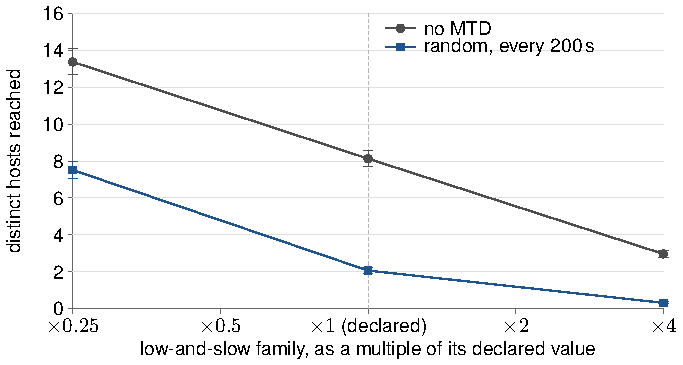
\includegraphics[width=0.78\textwidth]{fig_C-1a_sens_dwell_family}
  % CAPTION DRAFT STATE 2026-09-17 --- voice pass owed.
% [CONNECTIVE-PROSE PASS 2026-09-26, DS appendix caption] Marc 2026-09-26:
%  'deployment strategies is very clear ... change everything to
%  deployment strategies' (registry row re-ruled). SESSION-GENERATED on
%  Marc's 2026-09-26 go-ahead (docs/workflows/connective_prose.md; audit
%  docs/implementation/connective_prose_audit.md); prior text in git.
%  RATIFIED 2026-09-26 (Marc: 'I accept all this').
  \caption[NCR against the 45\,s mean duration]{NCR
  (Section~\ref{sec:evaluation-metrics}) as the mean duration of persistence, stealth and command and control
  is moved from 11.25 to 180\,s, the other mean durations held, with no MTD and
  under the random deployment strategy every 200\,s. Averaged over the four
  attack profiles, 400 runs per point; intervals are 95\,\%.}
  \label{fig:sens-dwell-anchor}
\end{figure}

\section{The exponential delay}
\label{app:exponential-shape}

% [prose slot --- Marc] the shape defence. The spine, from
%   stochastic_timing_design.md §3.1-3.3 and the note
%   docs/notes/ch4_methods/exponential_as_tractability_choice.md:
%     - what the exponential assumes: memorylessness, a mode at zero, and a
%       coefficient of variation fixed at 1;
%     - where it is defensible: the scan- and exploit-shaped tactics under a
%       retry-until-success reading;
%     - where it is plainly wrong: the low-and-slow group, whose defining
%       character is sustained, paced dwell --- mass concentrated AROUND a
%       value, which is the opposite of a mode-at-zero draw;
%     - why it is nonetheless the choice: the field defends the formalism,
%       not the shape. No surveyed stochastic-net paper defends
%       memorylessness as faithful to attacker behaviour, and the
%       substrate's own lineage switched to an exponential without
%       recording a justification at all. The claim here is a tractable,
%       precedented family, never a fidelity claim;
%     - the strongest available defence AND its named leak (madan2004: a
%       mean-time result can depend only on the sojourn means, PROVIDED
%       routing is independent of dwell --- which here it is not, because a
%       mutation races the dwell, so a long dwell is likelier to be
%       interrupted and shape re-enters through the interrupt channel);
%     - the counter-evidence, acknowledged not buried: holm2014's 203 025
%       intrusions find a Pareto best fit and report the exponential a poor
%       choice for time-to-compromise. Two qualifications travel with it:
%       opportunistic enterprise alarms rather than targeted campaigns, and
%       campaign-level rather than per-tactic timing.
%
%   The measured answer is Table~\ref{tab:shape-substitution}, and the claim
%   it licenses is deliberately narrow: the mean remains load-bearing across
%   the operating region and at every other cell tested, and it stops being
%   sufficient at the long-dwell corner under mutation pressure. That is
%   narrower than "shape matters" and stronger than the pre-S3-R sweep could
%   say. Worth stating plainly: the more behaviourally faithful shape is
%   WORSE for the attacker, because removing the exponential's near-zero
%   mass removes the short dwells that let an action complete between
%   mutations --- the property flagged as its least realistic feature is
%   quietly doing work.

% LEAD DRAFT STATE 2026-09-17 --- connective prose (green-lit), ratify-on-read.
% [DRAFT STATE 2026-10-05, with Section 4.4.2 round 5: "draw" and the family
%  names retired (Marc: "we don't use that word anymore").]
Each tactic duration is an exponential delay whose mean is the tactic's mean
duration (Section~\ref{subsec:dwell-times}). Here an Erlang-4 delay, the sum
of four exponential delays of a quarter of the mean, keeps each mean and varies
less. It replaces the exponential delay on the tactics with a 45\,s mean
duration and those set at half of it, paired run for run with the exponential
delay at 45\,s and at the top of the band, 180\,s.

% GENERATED by data/results/ch5_s51_sensitivity/analyse.py from
%   data/results/ch5_s51_sensitivity/numbers.json (the §5.1 re-run at the
%   chapter's pins; the attacker model pooled over its four profiles, 400 runs
%   per cell). Do not hand-edit; regenerate.

\begin{table}[htbp]
\centering\footnotesize
% CAPTION DRAFT STATE 2026-09-17 --- voice pass owed.
\caption[A less variable delay of the same mean]{NCR (Section~\ref{sec:evaluation-metrics}) under an Erlang-4 delay against the declared exponential delay, of the same mean, on the tactics with a 45\,s mean duration and those set at half of it, paired by attack profile and seed, at 45\,s and at the top of its band, 180\,s. Averaged over $c_1$ to $c_4$, 400 pairs per cell; $\pm$: a 95\,\% interval on the mean (normal approximation); each column is rounded to the precision of its widest interval. The last column counts the pairs in which the run under the Erlang-4 delay compromised fewer, the same, and more hosts.}
\label{tab:shape-substitution}
\tablestyle\setlength{\tabcolsep}{4pt}
\begin{tabular}{@{}P{2.0cm}P{2.4cm}>{\centering\arraybackslash}p{2.3cm}>{\centering\arraybackslash}p{2.3cm}>{\centering\arraybackslash}p{2.3cm}>{\centering\arraybackslash}p{2.6cm}@{}}
\toprule
Mean duration & MTD & Erlang-4 & Exponential & Difference & Pairs lower / tied / higher \\
\midrule
45\,s & no MTD & $0.162 \pm 0.008$ & $0.163 \pm 0.008$ & $0.000 \pm 0.001$ & 39 / 330 / 31 \\
 & random, 200\,s & $0.037 \pm 0.003$ & $0.041 \pm 0.004$ & $-0.005 \pm 0.004$ & 170 / 91 / 139 \\
 & random, 2\,000\,s & $0.147 \pm 0.007$ & $0.148 \pm 0.008$ & $-0.001 \pm 0.008$ & 175 / 54 / 171 \\
\midrule
180\,s & no MTD & $0.059 \pm 0.004$ & $0.059 \pm 0.004$ & $0.000 \pm 0.001$ & 40 / 321 / 39 \\
 & random, 200\,s & $0.006 \pm 0.001$ & $0.006 \pm 0.001$ & $-0.001 \pm 0.001$ & 73 / 269 / 58 \\
 & random, 2\,000\,s & $0.038 \pm 0.003$ & $0.041 \pm 0.003$ & $-0.003 \pm 0.003$ & 144 / 134 / 122 \\
\bottomrule
\end{tabular}
\end{table}


\section{Robustness across the failure matrix's decay parameters}
\label{app:decay-robustness}

% ADDED 2026-09-13 (stage-2 float audit, ch5 design handoff §18): the failure
% matrix's band-ends table, in the form tab:anchor-sensitivity already has, so
% that the body chapter draws no figure of a non-event. DATA: the weight
% sensitivity study RE-RUN at the reported configuration under the settled
% timing regime; the study on record
% (docs/implementation/pipeline/ogasp/weight_sensitivity_study.md) ran under the
% superseded fixed-dwell regime at ten seeds --- provenance, not values. The
% corner check on the influential pair is a row group here.
% [prose slot --- Marc] one framing paragraph: what is swept (the forward decay,
%   the backward decay and the floor over their declared bands, one at a time,
%   then the corners of the pair that proved most influential); what "inert"
%   means (band ends inside the interval at centre); and the honest limit the
%   record names (a finer per-profile ordering that fails to separate for want
%   of runs rather than of effect).
% LEAD DRAFT STATE 2026-09-17 --- connective prose (green-lit), ratify-on-read.
The distance term of the failure matrix (Section~\ref{subsec:failure-matrix},
Appendix~\ref{app:weight-sets}) has three numbers: the rate at which a jump
forward across two stages is scaled down, the rate for a fall back, and the
floor below which a factor reads as zero. Each was moved across its band with
the other two held, and the two rates were then run at their four corners
with the floor declared.

% GENERATED by data/results/ch5_s51_sensitivity/analyse.py from
%   data/results/ch5_s51_sensitivity/numbers.json (the §5.1 re-run at the
%   chapter's pins; the attacker model pooled over its four profiles, 400 runs
%   per cell). Do not hand-edit; regenerate.

\begin{table}[htbp]
\centering\footnotesize
% CAPTION DRAFT STATE 2026-09-17 --- voice pass owed.
\caption[NCR across the failure matrix's distance parameters]{NCR (Section~\ref{sec:evaluation-metrics}) at each distance parameter's band ends against its declared value, one at a time with the others held, and then at the four corners of the two rates with the floor declared, under no MTD and under the random deployment strategy at each interval. Averaged over the four profiles, 400 runs per cell; intervals are 95\,\%. The floor's rows are bit-identical to the declared point: no Petri net carries a jump of three stages, so its sensitivity is zero by structure rather than by measurement.}
\label{tab:decay-sensitivity}
\tablestyle\setlength{\tabcolsep}{4pt}
\begin{tabular}{@{}cP{3.4cm}>{\centering\arraybackslash}p{2.1cm}>{\centering\arraybackslash}p{2.1cm}>{\centering\arraybackslash}p{2.1cm}P{2.6cm}@{}}
\toprule
& Parameter & Band low & Declared & Band high & Verdict \\
\midrule
 & forward rate $\gamma$ (0.1, 0.5) & $0.165 \pm 0.009$ & $0.163 \pm 0.008$ & $0.164 \pm 0.008$ & inert \\
 & backward rate $\delta$ (0.1, 0.5) & $0.162 \pm 0.008$ & $0.163 \pm 0.008$ & $0.163 \pm 0.008$ & inert \\
 & floor $z$ (0, 0.05) & $0.163 \pm 0.008$ & $0.163 \pm 0.008$ & $0.163 \pm 0.008$ & zero by structure \\
 & corner $\gamma=0.1$, $\delta=0.1$ & --- & $0.163 \pm 0.008$ & $0.165 \pm 0.009$ & inert \\
 & corner $\gamma=0.1$, $\delta=0.5$ & --- & $0.163 \pm 0.008$ & $0.165 \pm 0.009$ & inert \\
 & corner $\gamma=0.5$, $\delta=0.1$ & --- & $0.163 \pm 0.008$ & $0.163 \pm 0.008$ & inert \\
\rowgroup{7}{no MTD} & corner $\gamma=0.5$, $\delta=0.5$ & --- & $0.163 \pm 0.008$ & $0.164 \pm 0.008$ & inert \\
\midrule
 & forward rate $\gamma$ (0.1, 0.5) & $0.044 \pm 0.004$ & $0.041 \pm 0.004$ & $0.042 \pm 0.004$ & inert \\
 & backward rate $\delta$ (0.1, 0.5) & $0.043 \pm 0.004$ & $0.041 \pm 0.004$ & $0.042 \pm 0.004$ & inert \\
 & floor $z$ (0, 0.05) & $0.041 \pm 0.004$ & $0.041 \pm 0.004$ & $0.041 \pm 0.004$ & zero by structure \\
 & corner $\gamma=0.1$, $\delta=0.1$ & --- & $0.041 \pm 0.004$ & $0.045 \pm 0.004$ & inert \\
 & corner $\gamma=0.1$, $\delta=0.5$ & --- & $0.041 \pm 0.004$ & $0.044 \pm 0.004$ & inert \\
 & corner $\gamma=0.5$, $\delta=0.1$ & --- & $0.041 \pm 0.004$ & $0.042 \pm 0.003$ & inert \\
\rowgroup{7}{random, 200\,s} & corner $\gamma=0.5$, $\delta=0.5$ & --- & $0.041 \pm 0.004$ & $0.044 \pm 0.004$ & inert \\
\midrule
 & forward rate $\gamma$ (0.1, 0.5) & $0.150 \pm 0.008$ & $0.148 \pm 0.008$ & $0.147 \pm 0.008$ & inert \\
 & backward rate $\delta$ (0.1, 0.5) & $0.150 \pm 0.008$ & $0.148 \pm 0.008$ & $0.151 \pm 0.008$ & inert \\
 & floor $z$ (0, 0.05) & $0.148 \pm 0.008$ & $0.148 \pm 0.008$ & $0.148 \pm 0.008$ & zero by structure \\
 & corner $\gamma=0.1$, $\delta=0.1$ & --- & $0.148 \pm 0.008$ & $0.149 \pm 0.008$ & inert \\
 & corner $\gamma=0.1$, $\delta=0.5$ & --- & $0.148 \pm 0.008$ & $0.152 \pm 0.008$ & inert \\
 & corner $\gamma=0.5$, $\delta=0.1$ & --- & $0.148 \pm 0.008$ & $0.146 \pm 0.008$ & inert \\
\rowgroup{7}{random, 2\,000\,s} & corner $\gamma=0.5$, $\delta=0.5$ & --- & $0.148 \pm 0.008$ & $0.149 \pm 0.008$ & inert \\
\bottomrule
\end{tabular}
\end{table}


\section{Robustness of attack confidentiality to the detector's memory}
\label{app:detector-memory}

% 2026-09-30: the placeholder described the retired tuned-alarm detector; filled
% on the count-in-window detector of Section 4.5.1 (ruling C). Numbers:
% ch5_s531_unopposed/numbers.json core.detector_grid, via
% tools/ch5_unopposed_figures.py. DRAFT STATE --- ratify on read.
Attack confidentiality (Section~\ref{subsec:metrics-behaviour}) flags an attack action
when it is at least the attacker's fifth within 60\,s, the default of the Snort
intrusion detection system \citep[Sec.~5.2]{jung2004}.
Table~\ref{tab:detector-memory} moves the count to three and ten and the window
to 30 and 120\,s. At the six settings that flag at least \prelim{2.5}\,\% of the
baseline attacker's attack actions, every attack profile keeps a higher attack
confidentiality than the baseline attacker. The other three flag under
\prelim{2}\,\% of its attack actions, and there the profiles lie within about one point
of it, above or below.

% GENERATED by tools/ch5_unopposed_figures.py from data/results/ch5_s531_unopposed/numbers.json
%   (core.detector_grid). Do not hand-edit; regenerate. 2026-09-30. DRAFT STATE --- ratify on read.
\begin{table}[htbp]
  \centering
  \caption[Attack confidentiality across the detector's count and window]{Attack confidentiality (\%) with no MTD running at each count and window of the scan detector (Section~\ref{subsec:metrics-behaviour}), for the APT attacker model on the attack profiles $c_1$ to $c_4$ and for the baseline attacker, with the share of the baseline attacker's actions each setting flags. The declared setting, five actions within 60\,s, is in bold. Every value's 95\,\% bootstrap interval over runs is within 2.4 points.}
  \label{tab:detector-memory}
  \tablestyle\setlength{\tabcolsep}{4pt}
  \begin{tabular}{@{}cc*{5}{>{\centering\arraybackslash}p{1.35cm}}>{\centering\arraybackslash}p{2.6cm}@{}}
    \toprule
    Count & Window (s) & $c_1$ & $c_2$ & $c_3$ & $c_4$ & \shortstack{baseline\\attacker} & Baseline attacker's actions flagged (\%) \\
    \midrule
    3 & 30 & 79.8 & 87.8 & 90.8 & 76.6 & 66.3 & 33.7 \\
    3 & 60 & 62.5 & 72.5 & 79.0 & 57.2 & 36.0 & 64.0 \\
    3 & 120 & 35.3 & 44.6 & 54.4 & 30.1 & 20.9 & 79.1 \\
    5 & 30 & 97.7 & 98.8 & 99.7 & 97.1 & 98.1 & 1.9 \\
    \textbf{5} & \textbf{60} & \textbf{92.0} & \textbf{95.9} & \textbf{98.1} & \textbf{89.4} & \textbf{82.6} & \textbf{17.4} \\
    5 & 120 & 74.6 & 84.3 & 90.4 & 67.6 & 52.5 & 47.5 \\
    10 & 30 & 100.0 & 100.0 & 100.0 & 100.0 & 100.0 & 0.0 \\
    10 & 60 & 99.9 & 100.0 & 100.0 & 99.9 & 100.0 & 0.0 \\
    10 & 120 & 99.3 & 99.6 & 100.0 & 98.7 & 97.5 & 2.5 \\
    \bottomrule
  \end{tabular}
\end{table}

% UPDATED 2026-09-24 (scrutinise-figure round 3, context critic): the alarm quantile
% matters --- at the 60th percentile c4 falls below the baseline attacker in the
% first 1 500 s bin (78.0 against 79.0), at the 75th c1 does too; at the median c4's
% first-bin margin is 4.6 pp (bootstrap 1.1-8.3). Sweep the quantile (e.g. 0.4-0.8)
% and tau together; theta_b depends on tau. §4.5 must say why the median.
% ALSO OWED (scrutinise-figure round 4, the examiner's first objection): the action rule.
% Counting dwell-only steps as actions brings the profiles level with the baseline
% (51-65 % against 50); counting every step makes c1, c2, c4 louder. Report the four
% variants as a table here (results context §8i-5); the claim is conditional on it.

% ADDED 2026-09-24 (Marc: "that's something that needs to be swept ... it has to
% be in the appendix, so make an appendix item for that"). The sweep is owed:
% tau over a band (e.g. 15-240 s, the declared 60 s inside it), both attackers,
% the no-defence corpus; the reading is the ordering of the attackers on attack
% confidentiality across the alarm levels, and the tau at which it changes, if
% any. A 2026-08 sweep exists for the older, tier-weighted form of the detector
% (data/misc/_viz/stealth_exposure/fig3_tau_sweep.png) and does not carry over.
% Brief: docs/handoffs/2026-09-24_s45_instrumenting_mtdsim.md, Open 4.



% [2026-09-30] Appendix 'Robustness of time lost to its window' deleted: time lost per MTD
% deployment now runs to the next deployment, so no window is declared (handoff
% 2026-09-30_disruption_metrics.md). Its table and generator are removed; history in git.


% =====================================================================
\chapter{MTDShield as run}
\label{app:mtdshield}

% DRAFT STATE 2026-09-25, SECOND CUT (Marc: "do we need to say so much ...
%  why don't we just make dot points for the changes ... properties, I don't
%  even know what that means"). Cut to the reuse report the field's checklists
%  ask for: what was taken and from where, which one and why, its settings, what
%  was changed, its known limitations. The first cut's argument (three ways of
%  choosing ranked; why the inputs are not rescaled; the loop rule) is reduced
%  to one sentence each; the long form is in git history (d6ab4b5a) and the
%  handoff 2026-09-22_ch5_defended_corpus_schemes_intervals_mtdshield.md §5.6-5.7.
%  Evidence: Tay's report §5.1-5.2, Figs 3-5; the release at f13ed49 / e6c13c6
%  (training script, evaluation builder and loop, notebook cells 1-3); the
%  weights read directly. Line numbers stay in the repo records, by ruling.
% OPEN FOR MARC: (1) the forced deployment keeps the simulator's random draw,
%  not the release's complete topology shuffle (last bullet of E.3); (2) the
%  release carries no licence file --- the reuse checklists ask for one to be
%  stated; permission through the supervisor, or a sentence saying it is
%  unlicensed and used with the author's knowledge. Ratify on read.
MTDShield in Chapter~\ref{ch:experiments} is one of Tay's trained agents, run
as released: his weights, and his code for building the agent's inputs
\citep{tay2024code}. This appendix gives which agent, its settings, what was
changed to run it and its known limitations.

\section{Selection}
\label{app:mtdshield-selection}

Tay trained 38 agents in three hyperparameter sweeps
(Table~\ref{tab:mtdshield-sweeps}) and scored each by summing five metrics,
attack success rate, mean time to compromise, attack path exposure, return on
attack and risk, each as a multiple of its value with no MTD
\citep[Sec.~5.1]{tay2024}. The agent run here is the one he scored highest:
initial exploration rate 0.5, decayed by 0.99 per episode, score 11.00
\citep[Sec.~5.2.2]{tay2024}. His report gives the sweep ranges but not every
setting held within them; those are read from the release's training script.
Re-scoring the agents, or retraining one, would make the choice this
dissertation's, so his designation is taken as it stands.

One caution attaches to it. Tay's scores were produced with the exploration
rate at one, so every scored run chose its mechanisms at random whichever agent
was loaded, and the scores do not separate the agents' policies. For the same
reason Chapter~\ref{ch:experiments} runs random selection over the same four
mechanisms beside MTDShield: Tay's figures compare MTDShield against it, and
the difference between the two is what the agent's policy adds.

\begin{table}[htbp]
  \centering
  \caption[Tay's hyperparameter sweeps]{Tay's three hyperparameter sweeps, the
  settings held in each, and the highest and lowest summed scores he reports
  \citep[Sec.~5.2, Figs.~3--5]{tay2024}. $\gamma$ is the discount factor and
  $\varepsilon$ the initial exploration rate; the training start is the number of
  stored transitions before learning begins. Held settings are from the
  release's training script \citep{tay2024code}. An empty cell was not reported.}
  \label{tab:mtdshield-sweeps}
  \tablestyle
  \begin{tabular}{@{}P{2.3cm}P{2.9cm}cP{3.3cm}P{2.2cm}P{2.0cm}@{}}
    \toprule
    Sweep & Values & Agents & Held & Highest & Lowest \\
    \midrule
    discount factor & $\gamma$ from 0.50 to 0.99 & 10 & $\varepsilon$ 1.0, decay 0.99; batch 64; training start 500 & 10.77 ($\gamma$ 0.85) & 9.46 ($\gamma$ 0.50) \\
    exploration & $\varepsilon$ from 0.5 to 1.0; decay from 0.980 to 0.998 & 24 & $\gamma$ 0.95; batch 32; training start 1\,000 & 11.00 ($\varepsilon$ 0.5, decay 0.99) & 9.48 ($\varepsilon$ 1.0, decay 0.980) \\
    training start & 500 to 2\,000 transitions & 4 & $\gamma$ 0.95; $\varepsilon$ 1.0, decay 0.99; batch 32 & 10.39 (2\,000) & \\
    \bottomrule
  \end{tabular}
\end{table}

\section{Settings}
\label{app:mtdshield-configuration}

Table~\ref{tab:mtdshield-configuration} gives the agent's settings in training,
in Tay's evaluation and in Chapter~\ref{ch:experiments}. The agent was trained
at a 200\,s decision tick; at the other five ticks its inputs are passed as
measured, not rescaled, because they describe the network as it is.

\begin{table}[htbp]
  \centering
  \caption[MTDShield's settings: trained, evaluated by Tay, and run here]{The
  agent's settings in training, in Tay's evaluation and in
  Chapter~\ref{ch:experiments}. The first two columns are from the release's
  training script and evaluation notebook \citep{tay2024code}; the third is
  Table~\ref{tab:experiment}. The detection rate is the share of decisions at
  which the agent is told the attacker's current attack action; a deployment is forced
  when 2\,000\,s pass without one.}
  \label{tab:mtdshield-configuration}
  \tablestyle
  \begin{tabular}{@{}P{2.5cm}P{4.2cm}P{3.6cm}P{4.3cm}@{}}
    \toprule
    Setting & Training & Tay's evaluation & Chapter~\ref{ch:experiments} \\
    \midrule
    Learning & $\gamma$ 0.95; batch 32; replay memory 2\,000; training start 1\,000; 100 episodes; target network copied every 10 episodes & & \\
    Exploration rate & 0.5, decayed by 0.99 per episode to 0.18 & 1 & 0 \\
    Mechanisms & \multicolumn{3}{P{13.0cm}@{}}{complete topology shuffle, IP shuffle, OS diversity, service diversity, or no operation} \\
    Hosts & 100, a new network each episode & 150, a new network each run & 50 \\
    Run length & 5\,000\,s per episode & 15\,000\,s & 15\,000\,s \\
    Decision tick & 200\,s & 200\,s & 50, 100, 200, 500, 1\,000 and 2\,000\,s \\
    Attacker & the baseline attacker & the baseline attacker & the baseline attacker; the APT attacker model \\
    Detection rate & 1 & 1 (0 to 1 in \citealp[Figure~6]{tay2024}) & 1 \\
    Forced deployment & after 2\,000\,s & after 2\,000\,s & after 2\,000\,s \\
    Runs & 100 episodes & 100 per agent & 1\,000 per combination \\
    \bottomrule
  \end{tabular}
\end{table}

\section{Changes made to run it}
\label{app:mtdshield-changes}

Two changes were made to run the agent, and neither alters the simulation; the third item is what was kept.
\begin{itemize}
  \item \textbf{Inputs.} The simulator as inherited builds five state and seven
  time-series inputs; Tay's agents take eight and three. His construction is
  restored as an option beside the current one, which stays the default. It
  reads state only, and draws one random number per decision, as the current
  construction does.
  \item \textbf{Doing nothing.} In the release, a decision to do nothing did not
  advance the simulated clock, so an agent that prefers it would never move on.
  The simulator used here waits for the next tick, as after a deployment.
  \item \textbf{Unchanged.} The decision loop is the simulator's, the same for
  every deployment strategy in Chapter~\ref{ch:experiments}. It enqueues one mechanism per
  decision (the release enqueued the chosen mechanism twice) and draws the forced
  deployment at random (the release forced complete topology shuffle).
\end{itemize}

\section{Known limitations}
\label{app:mtdshield-limitations}

Each is found in the release \citep{tay2024code} and left as it is; correcting
any would make the agent this dissertation's rather than Tay's.
\begin{itemize}
  \item The published scores were produced with the exploration rate at one
  (Section~\ref{app:mtdshield-selection}).
  \item Five inputs are built differently by the training and evaluation code.
  The evaluation code reads four of them, the host compromise ratio, attack
  success rate, time to compromise and deployment frequency, from copies of the
  records taken when the agent starts, so they are zero at every decision; the
  fifth, shortest-path variability, has another formula. The agent is run as the
  release evaluates it, and checked with the training code's inputs
  (Section~\ref{app:mtdshield-observed}).
  \item The batch-normalisation layers' stored variances are zero, which scales
  each such layer's output about 30-fold at inference.
  \item Doing nothing was never a learning target: no transition for it was
  stored in training.
  \item The detection input codes the attacker's current attack action. An unmapped
  tactic of the APT attacker model dispatches no attack action, so it reads as nothing detected, the same
  value as a missed detection.
  \item The agent was trained at one decision tick, against the baseline
  attacker, on 100-host networks (Table~\ref{tab:mtdshield-configuration}).
\end{itemize}

\section{Behaviour observed}
\label{app:mtdshield-observed}

% POPULATED 2026-09-25 from data/results/ch5_defended/numbers.json §shield
% (the per-decision ledger), PRELIMINARY at 100 seeds and two ticks; re-read at
% the reported seed count and six ticks. Record:
% docs/implementation/pipeline/ogasp/ch5_mtdshield_preliminary_findings.md.
% DRAFT STATE --- ratify on read.
Each run records the agent's decisions; the shares below are over 100 runs per
attacker and deployment interval, averaged over $c_1$ to $c_4$ for the APT attacker model.
\begin{itemize}
  \item At the 200\,s tick the agent chose service diversity at 76\,\% of
  decisions against the baseline attacker and 70\,\% against the APT attacker
  model, and did nothing at 23\,\% and 29\,\%. The other three mechanisms took
  under 1\,\% together, and under 1\,\% of deployments were forced.
  \item At the 2\,000\,s tick a decision to do nothing leaves more than 2\,000\,s
  without a deployment by the next tick, so that deployment is forced: 28\,\%
  and 18\,\% of decisions. Service diversity took 46\,\% and 65\,\%.
  \item The expectation written before the run was a near-constant selector of
  service diversity, falsified by a service-diversity share below 0.7 or a share
  doing nothing above 0.2 at 200\,s. The first part held and the second did not.
  \item With the training code's inputs, against the baseline attacker at
  200\,s, the agent chose service diversity at 79\,\% of decisions and its NCR
  reduction was 0.71 [0.67, 0.76], against 0.70 [0.65, 0.75] with the
  evaluation code's. Against the APT attacker model the training code stops in
  435 of 500 runs at 200\,s: it divides by the number of port scans, and the
  model compromises hosts without one.
\end{itemize}

% =====================================================================
% NEW 2026-09-25 (results context §8j-4; Marc agreed the intervals leave the body
% table): the per-attacker tables with every interval. Heading and placement are
% the session's; DRAFT STATE --- ratify on read. PRELIMINARY: 100 seeds.
\chapter{Supplementary results}
\label{app:supplementary-results}

% 2026-09-30 (Marc): the headline's values, moved from Section 5.3.2 with the ASP
%  reduction values beside them. SESSION-GENERATED sentences, DRAFT STATE.
Tables~\ref{tab:eff-interval-values} and~\ref{tab:eff-interval-values-asp} give the values
Figure~\ref{fig:eff-cross-arm} plots, at every deployment interval.

% GENERATED by tools/ch5_sweep_figures.py from data/results/ch5_defended/numbers.json
%   (sections sweep and sweep_asp; the APT attacker model pooled over its four profiles). Do not hand-edit.
% 2026-09-25 (Marc on the first draft: the rank grid's dashes and italics did not
%   read): the values themselves, grouped as the headline figure's panels.
% 2026-09-30 (Marc): moved from section 5.3.2 to Appendix F, the ASP reduction table beside it;
%   the body keeps the ranking table. DRAFT STATE --- ratify on read.
\begin{table}[htbp]
  \centering
  \caption[NCR reduction under each attacker, by MTD and deployment interval]{NCR reduction for each MTD mechanism and deployment strategy against the APT attacker model, averaged over $c_1$ to $c_4$, and against the baseline attacker, at each deployment interval; 1 is no host compromised, 0 is as many as with no MTD, and a negative value is more hosts compromised than with no MTD. Rows grouped as panels~(a) to~(f) of Figure~\ref{fig:eff-cross-arm}; a layer's row gives the mean it plots. Grey text: the 95\,\% percentile bootstrap interval includes zero; the APT attacker model's cells hold four times as many runs as the baseline attacker's.}
  \label{tab:eff-interval-values}
  \tablestyle\scriptsize\setlength{\tabcolsep}{3pt}\rowcolors{1}{}{}
  \begin{tabular}{@{}P{3.75cm}*{12}{>{\centering\arraybackslash}p{0.78cm}}@{}}
    \toprule
    & \multicolumn{6}{c}{APT attacker model} & \multicolumn{6}{c}{Baseline attacker} \\
    \cmidrule(lr){2-7}\cmidrule(lr){8-13}
    Deployment interval (s) & 50 & 100 & 200 & 500 & 1\,000 & 2\,000 & 50 & 100 & 200 & 500 & 1\,000 & 2\,000 \\
    \midrule
    \textit{host layer, mean} & $0.98$ & $0.97$ & $0.96$ & $0.78$ & $0.50$ & $0.22$ & $0.72$ & $0.53$ & $0.49$ & $0.15$ & \textcolor{black!55}{$0.04$} & \textcolor{black!55}{$-0.01$} \\
    \quad IP shuffle & $0.99$ & $0.97$ & $0.96$ & $0.81$ & $0.57$ & $0.33$ & $0.89$ & $0.70$ & $0.68$ & $0.38$ & $0.27$ & $0.16$ \\
    \quad complete topology shuffle & $0.98$ & $0.96$ & $0.96$ & $0.77$ & $0.45$ & $0.16$ & $0.54$ & $0.43$ & $0.41$ & \textcolor{black!55}{$0.07$} & \textcolor{black!55}{$-0.07$} & $-0.13$ \\
    \quad host topology shuffle & $0.99$ & $0.97$ & $0.96$ & $0.77$ & $0.46$ & $0.17$ & $0.73$ & $0.45$ & $0.40$ & \textcolor{black!55}{$0.01$} & \textcolor{black!55}{$-0.09$} & \textcolor{black!55}{$-0.07$} \\
    \midrule
    \textit{service layer, mean} & $0.34$ & $0.35$ & $0.21$ & $0.08$ & \textcolor{black!55}{$0.03$} & \textcolor{black!55}{$0.01$} & $0.97$ & $0.97$ & $0.82$ & $0.25$ & $0.18$ & $0.10$ \\
    \quad port shuffle & $0.35$ & $0.37$ & $0.20$ & \textcolor{black!55}{$0.05$} & \textcolor{black!55}{$0.04$} & \textcolor{black!55}{$0.00$} & $0.99$ & $0.99$ & $0.90$ & \textcolor{black!55}{$0.06$} & \textcolor{black!55}{$0.03$} & \textcolor{black!55}{$0.03$} \\
    \quad OS diversity & $0.16$ & $0.17$ & \textcolor{black!55}{$0.07$} & \textcolor{black!55}{$-0.01$} & \textcolor{black!55}{$-0.03$} & \textcolor{black!55}{$-0.01$} & $0.92$ & $0.93$ & $0.64$ & \textcolor{black!55}{$0.01$} & \textcolor{black!55}{$0.00$} & \textcolor{black!55}{$-0.03$} \\
    \quad service diversity & $0.51$ & $0.51$ & $0.36$ & $0.21$ & $0.09$ & \textcolor{black!55}{$0.04$} & $0.99$ & $0.99$ & $0.91$ & $0.66$ & $0.51$ & $0.30$ \\
    \midrule
    \multicolumn{13}{@{}l}{\textit{credentials}} \\
    \quad user shuffle & $-0.14$ & $-0.11$ & $-0.14$ & $-0.08$ & \textcolor{black!55}{$-0.06$} & \textcolor{black!55}{$-0.04$} & $0.47$ & \textcolor{black!55}{$0.02$} & \textcolor{black!55}{$-0.07$} & \textcolor{black!55}{$-0.11$} & \textcolor{black!55}{$-0.07$} & \textcolor{black!55}{$-0.08$} \\
    \midrule
    \multicolumn{13}{@{}l}{\textit{deployment strategies}} \\
    \quad random & $0.96$ & $0.90$ & $0.75$ & $0.43$ & $0.18$ & $0.09$ & $0.72$ & $0.49$ & $0.33$ & \textcolor{black!55}{$0.02$} & \textcolor{black!55}{$-0.04$} & \textcolor{black!55}{$-0.03$} \\
    \quad MTDShield & $0.42$ & $0.39$ & $0.28$ & $0.16$ & $0.09$ & \textcolor{black!55}{$0.03$} & $0.83$ & $0.82$ & $0.70$ & $0.40$ & $0.19$ & \textcolor{black!55}{$0.06$} \\
    \quad alternative & $0.94$ & $0.90$ & $0.72$ & $0.39$ & $0.15$ & \textcolor{black!55}{$0.03$} & $0.67$ & $0.59$ & $0.39$ & \textcolor{black!55}{$0.04$} & \textcolor{black!55}{$-0.04$} & \textcolor{black!55}{$-0.05$} \\
    \bottomrule
  \end{tabular}
\end{table}

\begin{table}[htbp]
  \centering
  \caption[ASP reduction under each attacker, by MTD and deployment interval]{ASP reduction for each MTD mechanism and deployment strategy against the APT attacker model, averaged over $c_1$ to $c_4$, and against the baseline attacker, at each deployment interval; 1 is no run compromising a target host, 0 is as many as with no MTD, and a negative value is more runs compromising a target host than with no MTD. Rows grouped as panels~(g) to~(l) of Figure~\ref{fig:eff-cross-arm}; a layer's row gives the mean it plots. Grey text: the 95\,\% percentile bootstrap interval includes zero; the APT attacker model's cells hold four times as many runs as the baseline attacker's.}
  \label{tab:eff-interval-values-asp}
  \tablestyle\scriptsize\setlength{\tabcolsep}{3pt}\rowcolors{1}{}{}
  \begin{tabular}{@{}P{3.75cm}*{12}{>{\centering\arraybackslash}p{0.78cm}}@{}}
    \toprule
    & \multicolumn{6}{c}{APT attacker model} & \multicolumn{6}{c}{Baseline attacker} \\
    \cmidrule(lr){2-7}\cmidrule(lr){8-13}
    Deployment interval (s) & 50 & 100 & 200 & 500 & 1\,000 & 2\,000 & 50 & 100 & 200 & 500 & 1\,000 & 2\,000 \\
    \midrule
    \textit{host layer, mean} & $1.00$ & $1.00$ & $1.00$ & $1.00$ & $0.92$ & $0.81$ & $0.83$ & $0.55$ & $0.49$ & $-0.22$ & \textcolor{black!55}{$-0.16$} & \textcolor{black!55}{$-0.08$} \\
    \quad IP shuffle & $1.00$ & $1.00$ & $1.00$ & $1.00$ & $0.78$ & $0.56$ & $0.93$ & $0.78$ & $0.66$ & \textcolor{black!55}{$-0.19$} & \textcolor{black!55}{$-0.17$} & \textcolor{black!55}{$-0.09$} \\
    \quad complete topology shuffle & $1.00$ & $1.00$ & $1.00$ & $1.00$ & $1.00$ & $0.92$ & $0.69$ & $0.28$ & $0.36$ & $-0.36$ & $-0.26$ & \textcolor{black!55}{$-0.14$} \\
    \quad host topology shuffle & $1.00$ & $1.00$ & $1.00$ & $1.00$ & $0.97$ & $0.97$ & $0.88$ & $0.59$ & $0.45$ & \textcolor{black!55}{$-0.10$} & \textcolor{black!55}{$-0.05$} & \textcolor{black!55}{$-0.02$} \\
    \midrule
    \textit{service layer, mean} & $0.79$ & $0.69$ & $0.51$ & \textcolor{black!55}{$0.22$} & \textcolor{black!55}{$0.22$} & \textcolor{black!55}{$0.14$} & $0.97$ & $0.96$ & $0.86$ & $0.28$ & $0.26$ & \textcolor{black!55}{$0.19$} \\
    \quad port shuffle & $0.89$ & $0.72$ & $0.53$ & \textcolor{black!55}{$0.25$} & \textcolor{black!55}{$0.19$} & \textcolor{black!55}{$0.22$} & $1.00$ & $1.00$ & $0.95$ & \textcolor{black!55}{$0.07$} & \textcolor{black!55}{$0.03$} & \textcolor{black!55}{$0.00$} \\
    \quad OS diversity & $0.53$ & \textcolor{black!55}{$0.42$} & \textcolor{black!55}{$0.19$} & \textcolor{black!55}{$0.00$} & \textcolor{black!55}{$0.00$} & \textcolor{black!55}{$-0.03$} & $0.90$ & $0.88$ & $0.62$ & \textcolor{black!55}{$-0.14$} & \textcolor{black!55}{$-0.10$} & \textcolor{black!55}{$-0.09$} \\
    \quad service diversity & $0.94$ & $0.94$ & $0.81$ & $0.42$ & $0.47$ & \textcolor{black!55}{$0.22$} & $1.00$ & $1.00$ & $1.00$ & $0.91$ & $0.84$ & $0.66$ \\
    \midrule
    \multicolumn{13}{@{}l}{\textit{credentials}} \\
    \quad user shuffle & \textcolor{black!55}{$-0.17$} & \textcolor{black!55}{$-0.33$} & \textcolor{black!55}{$-0.11$} & \textcolor{black!55}{$-0.06$} & \textcolor{black!55}{$-0.03$} & \textcolor{black!55}{$0.06$} & $0.71$ & \textcolor{black!55}{$0.00$} & \textcolor{black!55}{$-0.19$} & \textcolor{black!55}{$-0.14$} & $-0.29$ & \textcolor{black!55}{$-0.12$} \\
    \midrule
    \multicolumn{13}{@{}l}{\textit{deployment strategies}} \\
    \quad random & $1.00$ & $1.00$ & $1.00$ & $1.00$ & $0.78$ & $0.72$ & $0.78$ & $0.57$ & $0.34$ & \textcolor{black!55}{$0.14$} & \textcolor{black!55}{$-0.12$} & \textcolor{black!55}{$0.03$} \\
    \quad MTDShield & $0.86$ & $0.81$ & $0.69$ & $0.58$ & $0.50$ & \textcolor{black!55}{$0.28$} & $1.00$ & $0.97$ & $0.91$ & $0.69$ & $0.41$ & \textcolor{black!55}{$0.07$} \\
    \quad alternative & $1.00$ & $1.00$ & $1.00$ & $0.94$ & $0.81$ & \textcolor{black!55}{$0.42$} & $0.78$ & $0.64$ & $0.57$ & \textcolor{black!55}{$-0.03$} & \textcolor{black!55}{$-0.03$} & \textcolor{black!55}{$-0.05$} \\
    \bottomrule
  \end{tabular}
\end{table}


Tables~\ref{tab:full-movement} and~\ref{tab:full-baseline} give every metric of
Table~\ref{tab:eff-cross-arm} with its interval, for each attacker.

% 2026-10-02 (results_presentation_standard.md T4: cells never wrap): Tables F.3 and F.4 on one
%  landscape page, at the house type size, with room for the runs behind each MTTC.
\begin{landscape}
% GENERATED by tools/ch5_sweep_figures.py from data/results/ch5_defended/numbers_reported.json (section ranking).
%   Do not hand-edit. DRAFT STATE --- ratify on read. 2026-09-30: ASP reduction added; MTTC at a target host.
% 2026-10-02 (results_presentation_standard.md P1, P2, S1-S2, N1): NCR and MTTC to the precision rule;
%   the reference's rank and reductions blank; a dash an MTTC not reported; > 0.99 and < 0.01 at the bounds.
\begin{table}[H]
  \centering
  \caption[MTD mechanisms and deployment strategies against APT attacker model, with intervals]{Each MTD mechanism and deployment strategy deployed every 200\,s against the APT attacker model, its attack profiles $c_1$ to $c_4$ combined, on the same 1\,000 seeds, 4\,000 runs per row (1\,000 per attack profile), on the metrics of Table~\ref{tab:metrics}. Rank is from Table~\ref{tab:eff-cross-arm} (Scott--Knott ESD on the mean hosts compromised per seed): rows that share a rank are not told apart. The first row, no MTD, is the reference each reduction is taken against: its rank and reductions are blank. MTTC is taken over the runs that compromise a target host, of any attack profile for the APT attacker model, their number in parentheses. A dash marks an MTTC not reported: fewer than 10 runs compromise a target host. Brackets on ASP: a 95\,\% Clopper--Pearson interval; on a reduction: a 95\,\% percentile bootstrap interval over runs; $\pm$: a 95\,\% interval on the mean (normal approximation). Each column is rounded to the precision of its widest interval; $<$ and $>$ mark a value or half-width that would round to 0 or 1 without reaching it.}
  \label{tab:full-movement}
  \tablestyle
  \begin{tabular}{@{}P{4.7cm}>{\centering\arraybackslash}p{0.9cm}>{\centering\arraybackslash}p{4.0cm}>{\centering\arraybackslash}p{3.2cm}>{\centering\arraybackslash}p{2.6cm}>{\centering\arraybackslash}p{3.2cm}>{\centering\arraybackslash}p{3.2cm}@{}}
    \toprule
    MTD & Rank & ASP & ASP reduction & NCR & NCR reduction & MTTC (s) \\
    \midrule
    no MTD &  & $0.090$ [$0.082$, $0.100$] &  & $0.171 \pm 0.003$ &  & $10\,700 \pm 300$ (361) \\
    \midrule
    IP shuffle & 1 & $0.000$ [$0.000$, $0.001$] & $1.00$ [$1.00$, $1.00$] & $0.007 \pm {<}0.001$ & $0.96$ [$0.96$, $0.96$] & --- \\
    host topology shuffle & 1 & $0.000$ [$0.000$, $0.001$] & $1.00$ [$1.00$, $1.00$] & $0.008 \pm {<}0.001$ & $0.95$ [$0.95$, $0.96$] & --- \\
    complete topology shuffle & 1 & $0.000$ [$0.000$, $0.001$] & $1.00$ [$1.00$, $1.00$] & $0.008 \pm {<}0.001$ & $0.95$ [$0.95$, $0.96$] & --- \\
    random & 2 & ${<}0.001$ [${<}0.001$, $0.001$] & ${>}0.99$ [$0.99$, $1.00$] & $0.043 \pm 0.001$ & $0.75$ [$0.74$, $0.75$] & --- \\
    alternative & 3 & $0.001$ [${<}0.001$, $0.002$] & $0.99$ [$0.99$, $1.00$] & $0.049 \pm 0.001$ & $0.72$ [$0.71$, $0.72$] & --- \\
    service diversity & 4 & $0.015$ [$0.012$, $0.020$] & $0.83$ [$0.78$, $0.87$] & $0.109 \pm 0.002$ & $0.36$ [$0.35$, $0.38$] & $10\,900 \pm 700$ (61) \\
    MTDShield & 5 & $0.028$ [$0.023$, $0.034$] & $0.69$ [$0.62$, $0.75$] & $0.123 \pm 0.002$ & $0.28$ [$0.26$, $0.30$] & $10\,700 \pm 600$ (112) \\
    port shuffle & 6 & $0.043$ [$0.037$, $0.050$] & $0.52$ [$0.43$, $0.61$] & $0.137 \pm 0.002$ & $0.20$ [$0.18$, $0.21$] & $10\,900 \pm 400$ (172) \\
    OS diversity & 7 & $0.069$ [$0.061$, $0.077$] & $0.24$ [$0.11$, $0.35$] & $0.159 \pm 0.002$ & $0.07$ [$0.05$, $0.09$] & $10\,900 \pm 300$ (275) \\
    user shuffle & 8 & $0.121$ [$0.111$, $0.131$] & $-0.34$ [$-0.52$, $-0.19$] & $0.188 \pm 0.003$ & $-0.10$ [$-0.12$, $-0.08$] & $10\,800 \pm 300$ (483) \\
    \bottomrule
  \end{tabular}
\end{table}

% GENERATED by tools/ch5_sweep_figures.py from data/results/ch5_defended/numbers_reported.json (section ranking).
%   Do not hand-edit. DRAFT STATE --- ratify on read. 2026-09-30: ASP reduction added; MTTC at a target host.
% 2026-10-02 (results_presentation_standard.md P1, P2, S1-S2, N1): NCR and MTTC to the precision rule;
%   the reference's rank and reductions blank; a dash an MTTC not reported; > 0.99 and < 0.01 at the bounds.
\begin{table}[H]
  \centering
  \caption[MTD mechanisms and deployment strategies against baseline attacker, with intervals]{Each MTD mechanism and deployment strategy deployed every 200\,s against the baseline attacker, on the same 1\,000 seeds, 1\,000 runs per row, on the metrics of Table~\ref{tab:metrics}. Rank is from Table~\ref{tab:eff-cross-arm} (Scott--Knott ESD on the mean hosts compromised per seed): rows that share a rank are not told apart. The first row, no MTD, is the reference each reduction is taken against: its rank and reductions are blank. MTTC is taken over the runs that compromise a target host, of any attack profile for the APT attacker model, their number in parentheses. A dash marks an MTTC not reported: fewer than 10 runs compromise a target host. Brackets on ASP: a 95\,\% Clopper--Pearson interval; on a reduction: a 95\,\% percentile bootstrap interval over runs; $\pm$: a 95\,\% interval on the mean (normal approximation). Each column is rounded to the precision of its widest interval; $<$ and $>$ mark a value or half-width that would round to 0 or 1 without reaching it.}
  \label{tab:full-baseline}
  \tablestyle
  \begin{tabular}{@{}P{4.7cm}>{\centering\arraybackslash}p{0.9cm}>{\centering\arraybackslash}p{4.0cm}>{\centering\arraybackslash}p{3.2cm}>{\centering\arraybackslash}p{2.6cm}>{\centering\arraybackslash}p{3.2cm}>{\centering\arraybackslash}p{3.2cm}@{}}
    \toprule
    MTD & Rank & ASP & ASP reduction & NCR & NCR reduction & MTTC (s) \\
    \midrule
    no MTD &  & $0.64$ [$0.61$, $0.67$] &  & $0.496 \pm 0.012$ &  & $9\,000 \pm 200$ (643) \\
    \midrule
    service diversity & 1 & ${<}0.01$ [${<}0.01$, $0.01$] & ${>}0.99$ [$0.99$, $1.00$] & $0.041 \pm 0.003$ & $0.92$ [$0.91$, $0.92$] & --- \\
    port shuffle & 1 & $0.02$ [$0.01$, $0.03$] & $0.97$ [$0.95$, $0.98$] & $0.046 \pm 0.004$ & $0.91$ [$0.90$, $0.92$] & $4\,000 \pm 900$ (20) \\
    IP shuffle & 2 & $0.16$ [$0.14$, $0.18$] & $0.75$ [$0.72$, $0.79$] & $0.157 \pm 0.006$ & $0.68$ [$0.67$, $0.70$] & $7\,500 \pm 500$ (159) \\
    MTDShield & 2 & $0.05$ [$0.04$, $0.06$] & $0.92$ [$0.90$, $0.95$] & $0.157 \pm 0.007$ & $0.68$ [$0.67$, $0.70$] & $7\,200 \pm 1\,100$ (49) \\
    OS diversity & 2 & $0.22$ [$0.19$, $0.25$] & $0.66$ [$0.61$, $0.70$] & $0.158 \pm 0.010$ & $0.68$ [$0.66$, $0.70$] & $8\,700 \pm 500$ (220) \\
    complete topology shuffle & 3 & $0.40$ [$0.37$, $0.43$] & $0.38$ [$0.32$, $0.43$] & $0.287 \pm 0.007$ & $0.42$ [$0.40$, $0.44$] & $10\,300 \pm 300$ (398) \\
    alternative & 3 & $0.29$ [$0.26$, $0.32$] & $0.55$ [$0.50$, $0.60$] & $0.306 \pm 0.008$ & $0.38$ [$0.36$, $0.40$] & $10\,500 \pm 400$ (288) \\
    host topology shuffle & 3 & $0.33$ [$0.30$, $0.36$] & $0.49$ [$0.44$, $0.54$] & $0.309 \pm 0.008$ & $0.38$ [$0.36$, $0.40$] & $10\,500 \pm 300$ (328) \\
    random & 4 & $0.38$ [$0.35$, $0.41$] & $0.42$ [$0.36$, $0.47$] & $0.332 \pm 0.008$ & $0.33$ [$0.31$, $0.35$] & $10\,300 \pm 300$ (376) \\
    user shuffle & 5 & $0.74$ [$0.71$, $0.77$] & $-0.15$ [$-0.22$, $-0.09$] & $0.516 \pm 0.012$ & $-0.04$ [$-0.07$, $-0.01$] & $9\,200 \pm 200$ (741) \\
    \bottomrule
  \end{tabular}
\end{table}

\end{landscape}

% 2026-10-01 (Marc: "table 5.7 moves to the appendix"): the vulnerability
%  memory's pool sweep, in Table 5.6's form. SESSION-GENERATED sentence, DRAFT STATE.
% 2026-10-02 (Marc: "move it to appendix F"): the figure follows its table
%  here from Section 5.4.3, which keeps the hypothesis's verdict. Sentence
%  extended to name it. DRAFT STATE.
% 2026-10-02: the attack profiles' ablation over the whole grid, cited by
%  Section 5.4.1's outcome paragraph. SESSION-DRAFTED sentence, DRAFT STATE.
Table~\ref{tab:ablation-attack-profiles} gives the attack profiles' ablation
(Section~\ref{subsec:ablation-attack-profiles}) at every MTD mechanism,
deployment strategy and deployment interval.

% GENERATED by data/results/ch5_defended/partition_ablation.py from partition_ablation_numbers.json
% (n = 1 000); never hand-edit. Section 5.4.1's grid. Caption DRAFT STATE 2026-10-02, ratify on read.
\begin{table}[tp]
  \centering
  \caption[The APT attacker model with and without the attack profiles, at every MTD and interval]{Cohen's $d$ on NCR of the APT attacker model averaged over $c_1$ to $c_4$, minus the same model on the attack graph, on the same 1\,000 seeds, for every MTD mechanism and deployment strategy at every deployment interval (with no MTD, $-0.28$ [$-0.35$, $-0.22$]). Bold: the 95\,\% bootstrap interval over seeds lies wholly beyond $\pm 0.2$; $\dagger$: it crosses $\pm 0.2$; otherwise it lies within.}
  \label{tab:ablation-attack-profiles}
  \tablestyle
  \begin{tabular}{@{}lcccccc@{}}
    \toprule
    & \multicolumn{6}{c}{Deployment interval (s)} \\
    \cmidrule(lr){2-7}
    MTD & 50 & 100 & 200 & 500 & 1\,000 & 2\,000 \\
    \midrule
    IP shuffle & \bfseries\boldmath $-0.32$ & \bfseries\boldmath $-0.41$ & \bfseries\boldmath $-0.47$ & \bfseries\boldmath $-0.70$ & \bfseries\boldmath $-0.76$ & \bfseries\boldmath $-0.56$ \\
    complete topology shuffle & \bfseries\boldmath $-0.35$ & \bfseries\boldmath $-0.46$ & \bfseries\boldmath $-0.44$ & \bfseries\boldmath $-0.58$ & \bfseries\boldmath $-0.54$ & $-0.25$$^{\dagger}$ \\
    host topology shuffle & \bfseries\boldmath $-0.30$ & \bfseries\boldmath $-0.37$ & \bfseries\boldmath $-0.43$ & \bfseries\boldmath $-0.55$ & \bfseries\boldmath $-0.45$ & \bfseries\boldmath $-0.34$ \\
    port shuffle & $-0.22$$^{\dagger}$ & $-0.23$$^{\dagger}$ & $-0.21$$^{\dagger}$ & $-0.23$$^{\dagger}$ & $-0.26$$^{\dagger}$ & $-0.25$$^{\dagger}$ \\
    user shuffle & $-0.20$$^{\dagger}$ & $-0.20$$^{\dagger}$ & $-0.24$$^{\dagger}$ & \bfseries\boldmath $-0.27$ & $-0.24$$^{\dagger}$ & $-0.25$$^{\dagger}$ \\
    OS diversity & $-0.26$$^{\dagger}$ & $-0.26$$^{\dagger}$ & \bfseries\boldmath $-0.26$ & $-0.26$$^{\dagger}$ & \bfseries\boldmath $-0.28$ & $-0.21$$^{\dagger}$ \\
    service diversity & $-0.18$$^{\dagger}$ & $-0.19$$^{\dagger}$ & $-0.16$$^{\dagger}$ & $-0.14$$^{\dagger}$ & $-0.11$ & $-0.12$ \\
    \midrule
    random & \bfseries\boldmath $-0.49$ & \bfseries\boldmath $-0.47$ & \bfseries\boldmath $-0.54$ & \bfseries\boldmath $-0.36$ & \bfseries\boldmath $-0.35$ & $-0.25$$^{\dagger}$ \\
    MTDShield & $-0.09$ & $-0.11$ & $-0.14$$^{\dagger}$ & $-0.08$ & $-0.13$ & $-0.11$ \\
    alternative & \bfseries\boldmath $-0.51$ & \bfseries\boldmath $-0.57$ & \bfseries\boldmath $-0.47$ & \bfseries\boldmath $-0.33$ & $-0.25$$^{\dagger}$ & $-0.18$$^{\dagger}$ \\
    \bottomrule
  \end{tabular}
\end{table}


Figure~\ref{fig:ablation-memory} and Table~\ref{tab:ablation-memory} give the
vulnerability memory's ablation
(Section~\ref{subsec:ablation-vulnerability-memory}) at every number of services
per operating system.

\begin{figure}[tp]
  \centering
  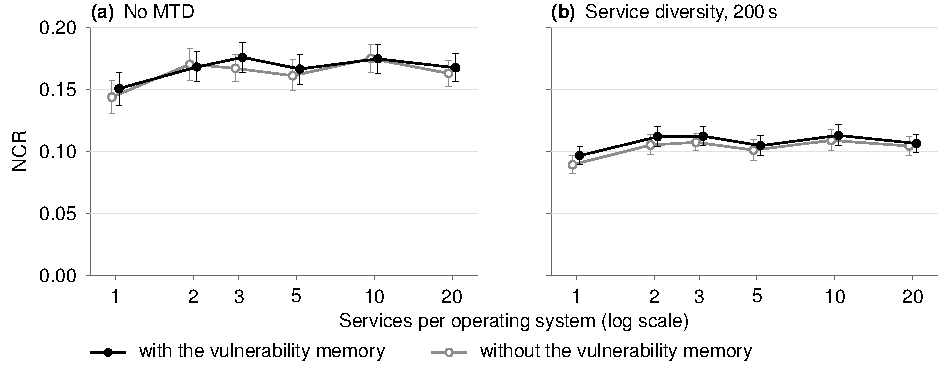
\includegraphics{fig_F-2_ablation_memory}
  % Generated by tools/ch5_memory_ablation_figure.py from
  % memory_ablation_numbers.json; takeaway and design record in its docstring.
  % Caption DRAFT STATE 2026-09-30, ratify on read. 2026-10-01: Figure 5.8
  %  becomes 5.7; one term (with and without, not on and off); bars over seeds,
  %  the unit Cohen's d uses; the pool sweep's table moved to Appendix F.
  %  2026-10-02: moved here from Section 5.4.3 (stem fig_5-4b -> fig_F-2).
  \caption[What removing the vulnerability memory changes]{NCR of the APT
  attacker model averaged over $c_1$ to $c_4$, with and without the
  vulnerability memory, on the same 1\,000 seeds, against the number of
  services per operating system, (a)~with no MTD and (b)~under service
  diversity at 200\,s. Bars are 95\,\% bootstrap intervals over seeds.
  Table~\ref{tab:ablation-memory} gives Cohen's $d$ at each pool, the share of
  exploits that succeed, and OS diversity.}
  \label{fig:ablation-memory}
\end{figure}

% GENERATED by data/results/ch5_defended/memory_ablation.py from memory_ablation_numbers.json;
% never hand-edit. Appendix F; the pool sweep behind fig:ablation-memory, in tab:ablation's form.
\begin{table}[tp]
  \centering
  \caption[The APT attacker model with and without the vulnerability memory, by services per operating system]{The APT attacker model with and without the vulnerability memory, averaged over $c_1$ to $c_4$, on the same 1\,000 seeds, by the number of services per operating system: the share of exploits that succeed, NCR, and $d$ on NCR, with minus without, with its 95\,\% percentile bootstrap interval over seeds. An exploit the host's operating system rules out is not counted.}
  \label{tab:ablation-memory}
  \tablestyle
  \begin{tabular}{@{}cccccc@{}}
    \toprule
    & \multicolumn{2}{c}{Exploits that succeed} & \multicolumn{3}{c}{NCR} \\
    \cmidrule(lr){2-3}\cmidrule(lr){4-6}
    \rowcolor{white}\shortstack{Services per\\operating system} & with & without & with & without & $d$ \\
    \midrule
    \grouprow{6}{no MTD} \\
    1 & 0.92 & 0.69 & 0.151 & 0.146 & $+$0.07 [$+$0.05, $+$0.10] \\
    2 & 0.87 & 0.69 & 0.162 & 0.157 & $+$0.09 [$+$0.06, $+$0.11] \\
    3 & 0.84 & 0.69 & 0.168 & 0.161 & $+$0.11 [$+$0.08, $+$0.13] \\
    5 & 0.80 & 0.70 & 0.170 & 0.167 & $+$0.05 [$+$0.02, $+$0.07] \\
    10 & 0.76 & 0.70 & 0.173 & 0.169 & $+$0.06 [$+$0.04, $+$0.09] \\
    20 & 0.73 & 0.69 & 0.171 & 0.169 & $+$0.04 [$+$0.02, $+$0.06] \\
    \addlinespace
    \grouprow{6}{service diversity, 200\,s} \\
    1 & 0.94 & 0.71 & 0.099 & 0.094 & $+$0.11 [$+$0.09, $+$0.14] \\
    2 & 0.91 & 0.70 & 0.104 & 0.099 & $+$0.12 [$+$0.10, $+$0.15] \\
    3 & 0.88 & 0.70 & 0.106 & 0.102 & $+$0.10 [$+$0.07, $+$0.12] \\
    5 & 0.84 & 0.71 & 0.108 & 0.104 & $+$0.10 [$+$0.08, $+$0.13] \\
    10 & 0.80 & 0.71 & 0.110 & 0.107 & $+$0.08 [$+$0.05, $+$0.10] \\
    20 & 0.76 & 0.71 & 0.109 & 0.106 & $+$0.07 [$+$0.05, $+$0.09] \\
    \addlinespace
    \grouprow{6}{OS diversity, 200\,s} \\
    1 & 0.93 & 0.70 & 0.140 & 0.134 & $+$0.09 [$+$0.06, $+$0.11] \\
    2 & 0.89 & 0.69 & 0.149 & 0.142 & $+$0.12 [$+$0.10, $+$0.15] \\
    3 & 0.86 & 0.70 & 0.156 & 0.149 & $+$0.13 [$+$0.10, $+$0.15] \\
    5 & 0.82 & 0.70 & 0.159 & 0.153 & $+$0.11 [$+$0.09, $+$0.14] \\
    10 & 0.78 & 0.70 & 0.162 & 0.157 & $+$0.08 [$+$0.05, $+$0.11] \\
    20 & 0.74 & 0.70 & 0.159 & 0.156 & $+$0.05 [$+$0.02, $+$0.07] \\
    \bottomrule
  \end{tabular}
\end{table}


\bibliography{references}

\end{document}
